\documentclass[
12pt,
openright,
twoside,
a4paper,
brazil
]{abntex2}
\usepackage[utf8]{inputenc}
\usepackage{indentfirst}
\usepackage[dvipsnames,x11names]{xcolor}
\usepackage{amsmath}
\usepackage{mathtools}
\usepackage{tikz}
\usepackage{siunitx}
\usepackage{algpseudocode}
\usepackage{algorithm}

\makeatletter
  \renewcommand{\ALG@name}{Algoritmo}
  \renewcommand{\algorithmicrequire}{\textbf{Entrada:}}
  \renewcommand{\algorithmicensure}{\textbf{Saída:}}
  \renewcommand{\listalgorithmname}{List of \ALG@name s}
\makeatother

\title{\textsc{Alocação de Polos Em Regiões do Plano Complexo via LMIs}}
\author{Alexandre Nascimento, Jr.}
\instituicao{Universidade Federal de Mato Grosso do Sul}
\local{Campo Grande, MS}

\begin{document}

\maketitle

\chapter{Introdução}

Notação:
\begin{itemize}
  \item $\Herm{(A)} = A + A'$;
  \item $\herm{(A)} = A - A'$
  \item $\loc(v_1, v_2)$ determina o ponto que a reta que passa por $v_1$ e $v_2$ cruza o eixo real;
  \item $\angulo(v_1, v_2)$ refere-se ao ângulo entre aquela reta e o eixo real.
\end{itemize}
\chapter{Região de Desempenho Garantido}

A alocação de polos é uma das principais ferramentas da teoria de controle, pois a partir desta, é possível projetar um sistema que seja estável e que tenha um bom desempenho \cite{ROSINOVA2014}. A operação de alocar polos de um sistema linear dentro de uma região específica é chamada $\mathscr{D}$-estabilidade \cite{WISNIEWSKI2017}.

Entende-se por estável o sistema que, em termos de resposta a estímulos, possui uma convergência ao zero da resposta natural, restando apenas a reposta forçada \cite{NISE2011}. Assim, para um intervalo de tempo determinado, espera-se que o sistema apenas tenha dinâmica referente à entrada aplicada. Neste contexto, a estabilidade é o ponto de partida para projetos de compensadores.

Na $\mathscr{D}$-estabilidade, a região referente à estabilidade em sistema contínuos e invariantes no tempo é o semi-plano esquerdo do plano complexo. Dado um ponto genérico no plano $s$, representado por:
\begin{equation}
  s = x + jy\label{eq:PontoGenericoPlanoS}
\end{equation}
estará na região estável somente se a parte real de tal ponto estiver à esquerda do eixo imaginário, ou em números:
\begin{equation}
  \Re{(s)} < 0 \implies x < 0
\end{equation}

Assim, um sistema com $n$ polos é dito estável se todos os seus polos estão localizados à esquerda do eixo imaginário. A partir deste conceito, é possível definir estabilidade relativa. Se um sistema é estável para um valor $\sigma < 0$, então aquele é dito estável relativo (ao valor de $\sigma$). A figura \ref{subfig:EstabilidadeRelativaS} mostra um esboço da região comentada. À medida que o valor de $\sigma$ aumenta em valor absoluto, mais a esquerda a reta limitante se encontra e menor o plano estável relativo se torna.

Outros parâmetros de desempenho importantes para projetos de compensadores são o fator de amortecimento $\zeta$ e a frequência natural não-amortecida $\omega_n$. São caracterizados pela resposta de sistemas de segunda ordem à função impulso \cite{NISE2011}\cite{OGATA2011} e representam as oscilações não-amortecidas do modelo físico. Dado um polo representado como em \eqref{eq:PontoGenericoPlanoS}, é possível reescrever tal equação em termos de tais parâmetros:
\begin{equation}
  s = -\zeta\omega_n \pm \jmath\omega_n \sqrt {1-\zeta^2} \label{eq:PontoPlanoS}
\end{equation}
com $\sigma = -\zeta\omega_n$. As regiões de $\mathscr{D}$-estabilidade referente a tais parâmetros são obtidos fixando um deles em \eqref{eq:PontoPlanoS} e variando o outro em um certo intervalo. Por esse motivo, \eqref{eq:PontoPlanoS} pode ser entendido como uma função de duas varáveis, dado como:
\begin{equation}
  s(\zeta,\omega_n) = -\zeta\omega_n \pm \jmath\omega_n \sqrt {1-\zeta^2} \label{eq:FuncaoPontoPlanoS}
\end{equation}

\begin{figure}[!ht]
  \centering
  \begin{subfigure}[t]{0.3\columnwidth}
      % This file was created by matlab2tikz.
%
%The latest updates can be retrieved from
%  http://www.mathworks.com/matlabcentral/fileexchange/22022-matlab2tikz-matlab2tikz
%where you can also make suggestions and rate matlab2tikz.
%
\begin{tikzpicture}[scale = 0.48]

\begin{axis}[%
  axis lines=center,
  width=3.5in,
  height=3.5in,
  scale only axis,
  xmin=-0.55,
  xmax=0.07,
  ymin=-0.5,
  ymax=0.5,
  xtick=\empty,
  ytick=\empty,
  xticklabel style={anchor=south west, draw=none},
  xlabel={$X$},
  ylabel={$jY$},
  x label style={anchor=north}
]
\addplot [color=black, dashed, forget plot]
  table[row sep=crcr]{%
-0.05	-0.5\\
-0.05	0.5\\
};
\addplot [color=black, dashed, forget plot]
  table[row sep=crcr]{%
-0.1	-0.5\\
-0.1	0.5\\
};
\addplot [color=black, dashed, forget plot]
  table[row sep=crcr]{%
-0.15	-0.5\\
-0.15	0.5\\
};
\addplot [color=black, dashed, forget plot]
  table[row sep=crcr]{%
-0.2	-0.5\\
-0.2	0.5\\
};
\addplot [color=black, dashed, forget plot]
  table[row sep=crcr]{%
-0.25	-0.5\\
-0.25	0.5\\
};
\addplot [color=black, dashed, forget plot]
  table[row sep=crcr]{%
-0.3	-0.5\\
-0.3	0.5\\
};
\addplot [color=black, dashed, forget plot]
  table[row sep=crcr]{%
-0.35	-0.5\\
-0.35	0.5\\
};
\addplot [color=black, dashed, forget plot]
  table[row sep=crcr]{%
-0.4	-0.5\\
-0.4	0.5\\
};
\addplot [color=black, dashed, forget plot]
  table[row sep=crcr]{%
-0.45	-0.5\\
-0.45	0.5\\
};
\addplot [color=black, dashed, forget plot]
  table[row sep=crcr]{%
-0.5	-0.5\\
-0.5	0.5\\
};
\end{axis}

\draw (6.8,3.9) node[scale = 0.505, anchor=south] {\small $\sigma_1$};
\draw (0.4,3.9) node[scale = 0.505, anchor=south] {\small $\sigma_2$};

\end{tikzpicture}%
      \caption{}
      \label{subfig:EstabilidadeRelativaS}
  \end{subfigure}
  \begin{subfigure}[t]{0.3\columnwidth}
      % This file was created by matlab2tikz.
%
%The latest updates can be retrieved from
%  http://www.mathworks.com/matlabcentral/fileexchange/22022-matlab2tikz-matlab2tikz
%where you can also make suggestions and rate matlab2tikz.
%
\begin{tikzpicture}

\begin{axis}[%
  axis lines=center,
  width=3.5in,
  height=3.5in,
  scale only axis,
  xmin=-0.7,
  xmax=0.07,
  ymin=-0.5,
  ymax=0.5,
  xtick=\empty,
  ytick=\empty,
  xticklabel style={anchor=south west},
  x label style={anchor=north},
  xlabel={$\pmb{X}$},
  ylabel={$\pmb{jY}$}
]
\addplot [color=black, dashed, forget plot]
  table[row sep=crcr]{%
-0	0\\
-0.0204124145231931	0.1\\
-0.0408248290463863	0.2\\
-0.0612372435695794	0.3\\
-0.0816496580927726	0.4\\
-0.102062072615966	0.5\\
};
\addplot [color=black, dashed, forget plot]
  table[row sep=crcr]{%
-0	-0\\
-0.0204124145231931	-0.1\\
-0.0408248290463863	-0.2\\
-0.0612372435695794	-0.3\\
-0.0816496580927726	-0.4\\
-0.102062072615966	-0.5\\
};
\addplot [color=black, dashed, forget plot]
  table[row sep=crcr]{%
-0	0\\
-0.0314485451016576	0.1\\
-0.0628970902033151	0.2\\
-0.0943456353049727	0.3\\
-0.12579418040663	0.4\\
-0.157242725508288	0.5\\
};
\addplot [color=black, dashed, forget plot]
  table[row sep=crcr]{%
-0	-0\\
-0.0314485451016576	-0.1\\
-0.0628970902033151	-0.2\\
-0.0943456353049727	-0.3\\
-0.12579418040663	-0.4\\
-0.157242725508288	-0.5\\
};
\addplot [color=black, dashed, forget plot]
  table[row sep=crcr]{%
-0	0\\
-0.0436435780471985	0.1\\
-0.087287156094397	0.2\\
-0.130930734141595	0.3\\
-0.174574312188794	0.4\\
-0.218217890235992	0.5\\
};
\addplot [color=black, dashed, forget plot]
  table[row sep=crcr]{%
-0	-0\\
-0.0436435780471985	-0.1\\
-0.087287156094397	-0.2\\
-0.130930734141595	-0.3\\
-0.174574312188794	-0.4\\
-0.218217890235992	-0.5\\
};
\addplot [color=black, dashed, forget plot]
  table[row sep=crcr]{%
-0	0\\
-0.0577350269189626	0.1\\
-0.115470053837925	0.2\\
-0.173205080756888	0.3\\
-0.23094010767585	0.4\\
-0.288675134594813	0.5\\
};
\addplot [color=black, dashed, forget plot]
  table[row sep=crcr]{%
-0	-0\\
-0.0577350269189626	-0.1\\
-0.115470053837925	-0.2\\
-0.173205080756888	-0.3\\
-0.23094010767585	-0.4\\
-0.288675134594813	-0.5\\
};
\addplot [color=black, dashed, forget plot]
  table[row sep=crcr]{%
-0	0\\
-0.075	0.1\\
-0.15	0.2\\
-0.225	0.3\\
-0.3	0.4\\
-0.375	0.5\\
};
\addplot [color=black, dashed, forget plot]
  table[row sep=crcr]{%
-0	-0\\
-0.075	-0.1\\
-0.15	-0.2\\
-0.225	-0.3\\
-0.3	-0.4\\
-0.375	-0.5\\
};
\addplot [color=black, dashed, forget plot]
  table[row sep=crcr]{%
-0	0\\
-0.0980196058819607	0.1\\
-0.196039211763921	0.2\\
-0.294058817645882	0.3\\
-0.392078423527843	0.4\\
-0.490098029409803	0.5\\
};
\addplot [color=black, dashed, forget plot]
  table[row sep=crcr]{%
-0	-0\\
-0.0980196058819607	-0.1\\
-0.196039211763921	-0.2\\
-0.294058817645882	-0.3\\
-0.392078423527843	-0.4\\
-0.490098029409803	-0.5\\
};
\addplot [color=black, dashed, forget plot]
  table[row sep=crcr]{%
-0	0\\
-0.133333333333333	0.1\\
-0.266666666666667	0.2\\
-0.4	0.3\\
-0.533333333333334	0.4\\
-0.666666666666667	0.5\\
};
\addplot [color=black, dashed, forget plot]
  table[row sep=crcr]{%
-0	-0\\
-0.133333333333333	-0.1\\
-0.266666666666667	-0.2\\
-0.4	-0.3\\
-0.533333333333334	-0.4\\
-0.666666666666667	-0.5\\
};
\end{axis}

\draw (7.3,8.4) node[anchor=south] {\small $\zeta_1$};
\draw (1.2,8.4) node[anchor=south] {\small $\zeta_2$};

\end{tikzpicture}%
      \caption{}
      \label{subfig:TaxaDeAmortecimentoS}
  \end{subfigure}
  \begin{subfigure}[t]{0.35\columnwidth}
    % This file was created by matlab2tikz.
%
%The latest updates can be retrieved from
%  http://www.mathworks.com/matlabcentral/fileexchange/22022-matlab2tikz-matlab2tikz
%where you can also make suggestions and rate matlab2tikz.
%
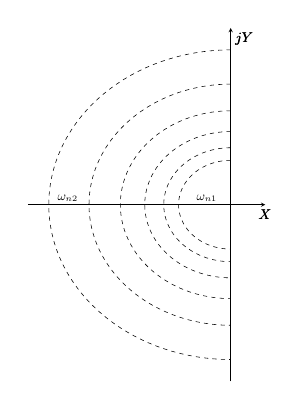
\begin{tikzpicture}[scale = 0.505]

\begin{axis}[%
  axis lines=center,
  width=2.35in,
  height=3.5in,
  scale only axis,
  xmin=-0.41,
  xmax=0.07,
  ymin=-0.42,
  ymax=0.42,
  xtick=\empty,
  ytick=\empty,
  xtick style={draw=none},
  ytick style={draw=none},
  xlabel={$\pmb{X}$},
  ylabel={$\pmb{jY}$},
  x label style={anchor=north}
]
\addplot [color=black, dashed, forget plot]
  table[row sep=crcr]{%
2.25261190051362e-17	0.367879441171442\\
-0.00367873309878077	0.367861047352666\\
-0.00735709832731729	0.367805867735705\\
-0.011034727852152	0.367713907838474\\
-0.014711253913397	0.367585176856886\\
-0.0183863088615101	0.367419687663933\\
-0.0220595251940588	0.367217456808395\\
-0.0257305355924711	0.36697850451319\\
-0.0293989729587661	0.366702854673348\\
-0.0330644704522643	0.366390534853623\\
-0.0367266615262709	0.366041576285738\\
-0.0403851799647304	0.365656013865257\\
-0.0440396599188475	0.365233886148102\\
-0.0476897359436723	0.364775235346693\\
-0.0513350430346442	0.364280107325728\\
-0.0549752166640916	0.363748551597596\\
-0.0586098928176851	0.363180621317427\\
-0.0622387080308383	0.362576373277775\\
-0.0658612994250539	0.361935867902942\\
-0.0694773047442111	0.361259169242931\\
-0.0730863623907915	0.360546344967044\\
-0.0766881114620379	0.359797466357114\\
-0.0802821917860447	0.359012608300379\\
-0.0838682439577744	0.35819184928199\\
-0.0874459093749984	0.357335271377165\\
-0.0910148302741562	0.356442960242981\\
-0.094574649766132	0.355515005109807\\
-0.0981250118719431	0.354551498772384\\
-0.101665561558338	0.353552537580542\\
-0.105195944773297	0.352518221429568\\
-0.108715808481443	0.351448653750216\\
-0.112224800699336	0.350343941498361\\
-0.11572257053068	0.349204195144309\\
-0.119208768201406	0.348029528661745\\
-0.122683045094652	0.346820059516338\\
-0.126145053785624	0.345575908653996\\
-0.129594448076338	0.344297200488767\\
-0.13303088303024	0.342984062890402\\
-0.136454015006697	0.341636627171568\\
-0.139863501695365	0.340255028074712\\
-0.143259002150416	0.338839403758595\\
-0.146640176824634	0.337389895784466\\
-0.150006687603369	0.335906649101916\\
-0.153358197838349	0.334389812034378\\
-0.156694372381343	0.332839536264293\\
-0.160014877617677	0.331255976817947\\
-0.163319381499595	0.329639292049965\\
-0.166607553579462	0.327989643627477\\
-0.16987906504281	0.32630719651395\\
-0.173133588741219	0.324592118952693\\
-0.176370799225032	0.322844582450033\\
-0.179590372775897	0.321064761758165\\
-0.182791987439143	0.319252834857673\\
-0.185975323055971	0.317408982939739\\
-0.189140061295473	0.315533390388018\\
-0.192285885686461	0.313626244760202\\
-0.195412481649118	0.311687736769264\\
-0.198519536526453	0.309718060264388\\
-0.201606739615568	0.307717412211583\\
-0.204673782198727	0.305685992673987\\
-0.207720357574227	0.303624004791861\\
-0.210746161087069	0.301531654762275\\
-0.213750890159423	0.299409151818489\\
-0.216734244320887	0.297256708209027\\
-0.21969592523853	0.295074539176458\\
-0.222635636746728	0.292862862935866\\
-0.225553084876781	0.290621900653031\\
-0.228447977886306	0.288351876422316\\
-0.231320026288416	0.28605301724425\\
-0.234168942880662	0.283725553002837\\
-0.236994442773761	0.281369716442561\\
-0.239796243420077	0.278985743145115\\
-0.24257406464188	0.276573871505841\\
-0.245327628659364	0.274134342709894\\
-0.248056660118421	0.271667400708121\\
-0.250760886118179	0.269173292192666\\
-0.253440036238292	0.266652266572302\\
-0.256093842565981	0.26410457594749\\
-0.258722039722823	0.26153047508517\\
-0.261324364891295	0.258930221393282\\
-0.263900557841047	0.25630407489503\\
-0.266450360954931	0.253652298202874\\
-0.268973519254761	0.250975156492274\\
-0.271469780426809	0.24827291747517\\
-0.273938894847039	0.245545851373212\\
-0.276380615606066	0.242794230890738\\
-0.278794698533848	0.240018331187502\\
-0.281180902224105	0.237218429851162\\
-0.283538988058457	0.234394806869519\\
-0.285868720230284	0.231547744602517\\
-0.288169865768311	0.22867752775401\\
-0.290442194559903	0.225784443343292\\
-0.292685479374072	0.222868780676393\\
-0.294899495884209	0.219930831317149\\
-0.297084022690505	0.216970889058049\\
-0.299238841342102	0.213989249890851\\
-0.301363736358929	0.210986211976989\\
-0.303458495253256	0.20796207561775\\
-0.305522908550938	0.20491714322425\\
-0.307556769812368	0.201851719287191\\
-0.309559875653112	0.198766110346413\\
-0.311532025764257	0.195660624960238\\
-0.313473022932435	0.192535573674617\\
-0.315382673059546	0.189391268992075\\
-0.317260785182169	0.186228025340458\\
-0.319107171490657	0.183046159041498\\
-0.320921647347918	0.17984598827917\\
-0.322704031307877	0.176627833067887\\
-0.324454145133625	0.173392015220486\\
-0.326171813815238	0.170138858316055\\
-0.327856865587277	0.166868687667575\\
-0.329509131945971	0.163581830289385\\
-0.331128447666061	0.160278614864484\\
-0.332714650817323	0.156959371711661\\
-0.334267582780765	0.153624432752466\\
-0.335787088264484	0.150274131478016\\
-0.337273015319199	0.146908802915647\\
-0.338725215353441	0.143528783595409\\
-0.340143543148418	0.140134411516418\\
-0.341527856872532	0.136726026113055\\
-0.342878018095565	0.133303968221017\\
-0.344193891802519	0.129868580043244\\
-0.34547534640712	0.126420205115691\\
-0.346722253764975	0.122959188272975\\
-0.347934489186388	0.119485875613898\\
-0.349111931448827	0.11600061446683\\
-0.350254462809047	0.112503753354983\\
-0.351361969014863	0.108995641961553\\
-0.352434339316579	0.105476631094757\\
-0.353471466478057	0.101947072652748\\
-0.354473246787446	0.0984073195884287\\
-0.35543958006755	0.0948577258741568\\
-0.356370369685845	0.0912986464663452\\
-0.357265522564147	0.0877304372699691\\
-0.358124949187912	0.0841534551029745\\
-0.358948563615195	0.0805680576605971\\
-0.359736283485239	0.0769746034795934\\
-0.360488030026714	0.0733734519023872\\
-0.361203728065591	0.0697649630411351\\
-0.361883306032665	0.0661494977417161\\
-0.362526695970703	0.0625274175476472\\
-0.36313383354125	0.0588990846639298\\
-0.363704658031052	0.0552648619208283\\
-0.364239112358138	0.0516251127375887\\
-0.364737143077519	0.047980201086096\\
-0.365198700386539	0.044330491454478\\
-0.365623738129852	0.0406763488106566\\
-0.366012213804037	0.0370181385658511\\
-0.366364088561851	0.0333562265380371\\
-0.366679327216111	0.0296909789153662\\
-0.366957898243215	0.0260227622195462\\
-0.367199773786291	0.0223519432691898\\
-0.367404929657988	0.018678889143133\\
-0.367573345342889	0.0150039671437274\\
-0.367705003999565	0.011327544760111\\
-0.367799892462262	0.00764998963145812\\
-0.367858001242211	0.00397166951021691\\
-0.367879324528583	0.000292952225334387\\
-0.367863860189067	-0.00338579435452654\\
-0.367811609770085	-0.0070642023577735\\
-0.367722578496634	-0.0107419039466713\\
-0.367596775271768	-0.0144185313541261\\
-0.367434212675705	-0.0180937169204609\\
-0.367234906964568	-0.0217670931301818\\
-0.366998878068762	-0.0254382926487287\\
-0.366726149590982	-0.0291069483592092\\
-0.366416748803846	-0.0327726933991097\\
-0.366070706647176	-0.0364351611969807\\
-0.365688057724899	-0.0400939855090944\\
-0.365268840301589	-0.0437488004560688\\
-0.364813096298638	-0.0473992405594549\\
-0.364320871290068	-0.0510449407782843\\
-0.363792214497968	-0.054685536545573\\
-0.363227178787577	-0.0583206638047783\\
-0.362625820661996	-0.0619499590462036\\
-0.361988200256536	-0.0655730593433491\\
-0.361314381332707	-0.0691896023892044\\
-0.360604431271838	-0.0727992265324783\\
-0.359858421068345	-0.0764015708137649\\
-0.359076425322625	-0.079996275001638\\
-0.358258522233603	-0.0835829796286742\\
-0.357404793590906	-0.0871613260273997\\
-0.356515324766686	-0.0907309563661567\\
-0.355590204707084	-0.094291513684886\\
-0.354629525923335	-0.0978426419308229\\
-0.353633384482518	-0.101383985994102\\
-0.352601879997946	-0.104915191743268\\
-0.351535115619208	-0.108435906060688\\
-0.350433198021854	-0.111945776877866\\
-0.349296237396724	-0.115444453210644\\
-0.348124347438933	-0.118931585194303\\
-0.346917645336501	-0.122406824118553\\
-0.345676251758632	-0.125869822462397\\
-0.344400290843651	-0.129320233928885\\
-0.343089890186584	-0.132757713479747\\
-0.341745180826406	-0.136181917369892\\
-0.340366297232932	-0.139592503181784\\
-0.338953377293372	-0.142989129859685\\
-0.337506562298543	-0.146371457743757\\
-0.336025996928739	-0.149739148604031\\
-0.334511829239262	-0.153091865674226\\
-0.332964210645621	-0.156429273685431\\
-0.331383295908384	-0.159751038899624\\
-0.329769243117708	-0.163056829143052\\
-0.328122213677528	-0.166346313839446\\
-0.326442372289413	-0.169619164043078\\
-0.324729886936105	-0.172875052471655\\
-0.32298492886471	-0.176113653539046\\
-0.321207672569581	-0.179334643387844\\
-0.319398295774868	-0.182537699921749\\
-0.317556979416742	-0.185722502837775\\
-0.315683907625304	-0.188888733658286\\
-0.313779267706173	-0.192036075762838\\
-0.311843250121753	-0.195164214419844\\
-0.309876048472189	-0.198272836818043\\
-0.307877859476007	-0.201361632097787\\
-0.305848882950442	-0.204430291382123\\
-0.303789321791454	-0.207478507807679\\
-0.301699381953445	-0.210505976555351\\
-0.299579272428655	-0.213512394880789\\
-0.297429205226271	-0.216497462144666\\
-0.295249395351222	-0.219460879842742\\
-0.293040060782677	-0.222402351635718\\
-0.290801422452254	-0.225321583378864\\
-0.288533704221919	-0.22821828315144\\
-0.286237132861606	-0.231092161285882\\
-0.283911938026537	-0.233942930396771\\
-0.281558352234257	-0.236770305409573\\
-0.279176610841386	-0.239574003589142\\
-0.276766952020077	-0.242353744567996\\
-0.274329616734204	-0.245109250374354\\
-0.271864848715264	-0.247840245459932\\
-0.269372894438007	-0.250546456727496\\
-0.266854003095782	-0.253227613558176\\
-0.264308426575626	-0.255883447838522\\
-0.261736419433068	-0.25851369398732\\
-0.25913823886668	-0.261118088982147\\
-0.256514144692353	-0.263696372385673\\
-0.253864399317318	-0.266248286371706\\
-0.251189267713904	-0.268773575750976\\
-0.248489017393042	-0.271271987996647\\
-0.245763918377515	-0.273743273269578\\
-0.243014243174952	-0.276187184443301\\
-0.240240266750583	-0.278603477128734\\
-0.237442266499739	-0.280991909698624\\
-0.234620522220113	-0.283352243311703\\
-0.23177531608378	-0.285684241936577\\
-0.228906932608985	-0.287987672375326\\
-0.226015658631685	-0.290262304286827\\
-0.223101783276867	-0.292507910209783\\
-0.220165597929638	-0.294724265585475\\
-0.217207396206088	-0.296911148780211\\
-0.214227473923922	-0.299068341107493\\
-0.211226129072887	-0.301195626849888\\
-0.208203661784965	-0.303292793280593\\
-0.205160374304367	-0.305359630684714\\
-0.202096570957305	-0.307395932380231\\
-0.199012558121561	-0.309401494738673\\
-0.195908644195848	-0.311376117205475\\
-0.192785139568971	-0.313319602320035\\
-0.189642356588792	-0.315231755735462\\
-0.186480609530989	-0.317112386238008\\
-0.183300214567632	-0.31896130576619\\
-0.180101489735568	-0.320778329429595\\
-0.176884754904615	-0.322563275527371\\
-0.173650331745575	-0.324315965566397\\
-0.170398543698069	-0.326036224279128\\
-0.167129715938191	-0.327723879641128\\
-0.163844175345993	-0.329378762888265\\
-0.160542250472797	-0.331000708533596\\
-0.157224271508339	-0.332589554383905\\
-0.15389057024775	-0.334145141555934\\
-0.150541480058377	-0.33566731449226\\
-0.14717733584645	-0.337155920976859\\
-0.143798474023585	-0.338610812150322\\
-0.14040523247315	-0.340031842524746\\
-0.136997950516471	-0.341418869998275\\
-0.133576968878905	-0.34277175586932\\
-0.130142629655766	-0.34409036485042\\
-0.126695276278112	-0.345374565081776\\
-0.123235253478409	-0.346624228144434\\
-0.119762907256055	-0.347839229073131\\
-0.116278584842777	-0.349019446368786\\
-0.112782634667913	-0.350164762010652\\
-0.109275406323567	-0.351275061468121\\
-0.105757250529652	-0.35235023371217\\
-0.102228519098815	-0.353390171226473\\
-0.0986895649012572	-0.354394770018144\\
-0.095140741829451	-0.355363929628141\\
-0.0915824047627455	-0.356297553141311\\
-0.0880149095318821	-0.35719554719608\\
-0.0844386128834111	-0.358057821993792\\
-0.0808538724440167	-0.358884291307685\\
-0.0772610466847562	-0.359674872491516\\
-0.0736604948852112	-0.360429486487827\\
-0.0700525770975613	-0.361148057835845\\
-0.0664376541105782	-0.361830514679036\\
-0.0628160874135489	-0.362476788772283\\
-0.0591882391601248	-0.363086815488716\\
-0.0555544721321081	-0.363660533826171\\
-0.0519151497031731	-0.364197886413293\\
-0.0482706358025306	-0.364698819515271\\
-0.0446212948785332	-0.365163283039212\\
-0.0409674918622322	-0.365591230539151\\
-0.0373095921308842	-0.365982619220694\\
-0.0336479614714146	-0.3663374099453\\
-0.0299829660438378	-0.366655567234192\\
-0.0263149723446422	-0.366937059271905\\
-0.022644347170141	-0.367181857909471\\
-0.0189714575797933	-0.36738993866723\\
-0.0152966708594972	-0.367561280737279\\
-0.0116203544848622	-0.367695866985555\\
-0.00794287608446205	-0.367793683953544\\
-0.00426460340307282	-0.367854721859632\\
-0.000585904264897101	-0.367878974600078\\
};
\addplot [color=black, dashed, forget plot]
  table[row sep=crcr]{%
1.75433591207597e-17	0.28650479686019\\
-0.00286500021804116	0.286490471739724\\
-0.00572971393844803	0.286447497810825\\
-0.0085938546922358	0.28637587937085\\
-0.0114571360677159	0.286275623581584\\
-0.0143192717391367	0.286146740468522\\
-0.0171799754953164	0.285989242919868\\
-0.0200389612682631	0.285803146685245\\
-0.0228959431617821	0.285588470374123\\
-0.0257506354800648	0.285345235453953\\
-0.0286027527562582	0.285073466248024\\
-0.0314520097810116	0.284773189933031\\
-0.0342981216309968	0.284444436536354\\
-0.0371408036974005	0.284087238933061\\
-0.0399797717143852	0.283701632842612\\
-0.0428147417875147	0.283287656825297\\
-0.0456454304221443	0.282845352278371\\
-0.0484715545517694	0.282374763431922\\
-0.0512928315663322	0.28187593734444\\
-0.0541089793404822	0.28134892389812\\
-0.0569197162617889	0.280793775793867\\
-0.0597247612589023	0.280210548546028\\
-0.0625238338296603	0.279599300476843\\
-0.0653166540691383	0.278960092710609\\
-0.0681029426976398	0.278292989167569\\
-0.0708824210886238	0.277598056557523\\
-0.0736548112965674	0.276875364373152\\
-0.0764198360847602	0.276124984883073\\
-0.0791772189530275	0.275346993124608\\
-0.0819266841653803	0.274541466896287\\
-0.0846679567775885	0.273708486750059\\
-0.0874007626646754	0.272848135983246\\
-0.0901248285483295	0.271960500630207\\
-0.0928398820242326	0.271045669453739\\
-0.0955456515892995	0.270103733936195\\
-0.0982418666688287	0.269134788270344\\
-0.100928257643559	0.268138929349944\\
-0.103604555876631	0.267116256760057\\
-0.106270493740453	0.266066872767091\\
-0.108925804643459	0.264990882308569\\
-0.111570223056772	0.263888392982641\\
-0.114203484540754	0.262759515037322\\
-0.116825325771451	0.261604361359464\\
-0.119435484566926	0.260423047463473\\
-0.122033699913472	0.259215691479755\\
-0.124619711991722	0.2579824141429\\
-0.127193262202622	0.256723338779617\\
-0.129754093193296	0.25543859129639\\
-0.132301948882779	0.254128300166899\\
-0.134836574487624	0.252792596419164\\
-0.137357716547384	0.251431613622446\\
-0.139865122949954	0.250045487873893\\
-0.142358542956783	0.248634357784922\\
-0.144837727227948	0.247198364467367\\
-0.147302427847088	0.245737651519364\\
-0.149752398346194	0.244252365010989\\
-0.152187393730259	0.242742653469657\\
-0.154607170501774	0.241208667865262\\
-0.157011486685077	0.239650561595087\\
-0.159400101850555	0.238068490468461\\
-0.16177277713868	0.236462612691177\\
-0.164129275283901	0.234833088849677\\
-0.166469360638369	0.233180081894984\\
-0.168792799195496	0.231503757126419\\
-0.171099358613364	0.229804282175059\\
-0.173388808237953	0.228081826986986\\
-0.175660919126208	0.226336563806281\\
-0.177915464068934	0.224568667157809\\
-0.180152217613516	0.22277831382976\\
-0.182370956086463	0.220965682855977\\
-0.184571457615776	0.219130955498046\\
-0.186753502153137	0.217274315227173\\
-0.18891687149591	0.215395947705839\\
-0.191061349308964	0.213496040769231\\
-0.193186721146304	0.211574784406458\\
-0.195292774472517	0.209632370741556\\
-0.197379298684027	0.207668994014274\\
-0.199446085130151	0.205684850560646\\
-0.201492927133966	0.203680138793367\\
-0.203519620012978	0.20165505918194\\
-0.205525961099588	0.199609814232641\\
-0.207511749761359	0.19754460846826\\
-0.209476787421079	0.195459648407651\\
-0.211420877576621	0.193355142545085\\
-0.213343825820589	0.191231301329392\\
-0.215245439859761	0.189088337142926\\
-0.217125529534317	0.186926464280318\\
-0.218983906836857	0.184745898927054\\
-0.2208203859312	0.182546859137852\\
-0.222634783170966	0.180329564814858\\
-0.224426917117943	0.178094237685656\\
-0.22619660856023	0.175841101281097\\
-0.227943680530157	0.173570380912944\\
-0.229667958321984	0.171282303651341\\
-0.231369269509368	0.168977098302108\\
-0.233047443962609	0.166654995383858\\
-0.234702313865658	0.164316227104948\\
-0.236333713732906	0.161961027340258\\
-0.237941480425724	0.159589631607801\\
-0.239525453168784	0.157202277045174\\
-0.24108547356613	0.154799202385844\\
-0.242621385617024	0.152380647935274\\
-0.244133035731541	0.149946855546894\\
-0.245620272745927	0.147498068597915\\
-0.247082947937722	0.14503453196499\\
-0.248520915040625	0.142556491999731\\
-0.249934030259123	0.140064196504069\\
-0.251322152282874	0.137557894705475\\
-0.252685142300831	0.135037837232043\\
-0.254022864015127	0.132504276087419\\
-0.255335183654708	0.129957464625605\\
-0.256621969988701	0.127397657525627\\
-0.257883094339547	0.12482511076606\\
-0.25911843059586	0.122240081599437\\
-0.260327855225045	0.119642828526521\\
-0.261511247285647	0.117033611270454\\
-0.262668488439446	0.114412690750788\\
-0.26379946296329	0.111780329057391\\
-0.26490405776067	0.109136789424237\\
-0.265982162373027	0.106482336203088\\
-0.267033668990797	0.103817234837054\\
-0.268058472464196	0.10114175183405\\
-0.26905647031373	0.0984561547401476\\
-0.270027562740445	0.0957607121128173\\
-0.270971652635908	0.0930556934940761\\
-0.271888645591917	0.0903413693835317\\
-0.27277844990994	0.0876180112113332\\
-0.273640976610286	0.0848858913110282\\
-0.274476139441005	0.0821452828923302\\
-0.275283854886509	0.0793964600137972\\
-0.276064042175926	0.0766396975554263\\
-0.276816623291179	0.0738752711911659\\
-0.277541522974782	0.071103457361349\\
-0.278238668737372	0.0683245332450487\\
-0.278907990864953	0.0655387767323608\\
-0.27954942242587	0.0627464663966151\\
-0.280162899277501	0.0599478814665182\\
-0.280748360072673	0.0571433017982312\\
-0.281305746265793	0.0543330078473837\\
-0.281835002118708	0.0515172806410286\\
-0.282336074706273	0.0486964017495403\\
-0.282808913921646	0.0458706532584575\\
-0.283253472481301	0.0430403177402742\\
-0.283669705929751	0.0402056782261836\\
-0.284057572643999	0.037367018177775\\
-0.284417033837696	0.0345246214586877\\
-0.284748053565023	0.031678772306225\\
-0.285050598724283	0.0288297553029306\\
-0.285324639061211	0.0259778553481305\\
-0.285570147172003	0.0231233576294437\\
-0.285787098506053	0.0202665475942635\\
-0.285975471368407	0.0174077109212127\\
-0.286135246921936	0.0145471334915759\\
-0.286266409189218	0.0116851013607126\\
-0.286368945054136	0.00882190072945083\\
-0.286442844263188	0.00595781791546771\\
-0.286488099426516	0.00309313932465775\\
-0.28650470601864	0.000228151422492931\\
-0.286492662378915	-0.00263685929462401\\
-0.286451969711696	-0.00550160632800887\\
-0.286382632086215	-0.00836580320534545\\
-0.286284656436176	-0.011229163509333\\
-0.286158052559064	-0.0140914009063273\\
-0.28600283311516	-0.0169522291749738\\
-0.285819013626279	-0.0198113622348295\\
-0.285606612474218	-0.0226685141749711\\
-0.285365650898913	-0.0255233992825857\\
-0.285096152996323	-0.0283757320715415\\
-0.284798145716013	-0.0312252273109363\\
-0.284471658858461	-0.034071600053621\\
-0.284116725072083	-0.0369145656646934\\
-0.283733379849961	-0.0397538398499613\\
-0.283321661526298	-0.0425891386843722\\
-0.282881611272582	-0.0454201786404055\\
-0.282413273093474	-0.0482466766164248\\
-0.281916693822399	-0.051068349964988\\
-0.281391923116872	-0.0538849165211115\\
-0.280839013453526	-0.0566960946304867\\
-0.280258020122866	-0.0595016031776455\\
-0.279649001223742	-0.0623011616140711\\
-0.279012017657535	-0.0650944899862528\\
-0.278347133122071	-0.0678813089636809\\
-0.277654414105251	-0.0706613398667803\\
-0.276933929878398	-0.0734343046947773\\
-0.276185752489335	-0.0761999261535\\
-0.275409956755176	-0.0789579276831068\\
-0.27460662025485	-0.0817080334857435\\
-0.273775823321336	-0.0844499685531214\\
-0.272917649033636	-0.0871834586940188\\
-0.272032183208464	-0.0899082305616993\\
-0.271119514391663	-0.092624011681247\\
-0.270179733849355	-0.095330530476813\\
-0.269212935558811	-0.0980275162987732\\
-0.268219216199055	-0.100714699450793\\
-0.267198675141194	-0.103391811216796\\
-0.266151414438484	-0.106058583887837\\
-0.265077538816122	-0.108714750788871\\
-0.263977155660775	-0.111360046305422\\
-0.262850375009843	-0.113994205910141\\
-0.261697309540451	-0.116616966189265\\
-0.260518074558185	-0.11922806486895\\
-0.259312787985562	-0.121827240841505\\
-0.258081570350233	-0.124414234191497\\
-0.256824544772936	-0.126988786221749\\
-0.255541836955181	-0.129550639479202\\
-0.254233575166682	-0.132099537780666\\
-0.252899890232527	-0.134635226238435\\
-0.251540915520098	-0.137157451285775\\
-0.250156786925733	-0.139665960702284\\
-0.24874764286114	-0.142160503639111\\
-0.247313624239549	-0.144640830644041\\
-0.245854874461628	-0.147106693686439\\
-0.244371539401139	-0.149557846182058\\
-0.242863767390353	-0.15199404301769\\
-0.241331709205213	-0.154415040575681\\
-0.239775518050262	-0.156820596758293\\
-0.238195349543318	-0.159210471011913\\
-0.236591361699916	-0.161584424351107\\
-0.234963714917502	-0.163942219382518\\
-0.233312571959399	-0.16628362032861\\
-0.231638097938526	-0.168608393051238\\
-0.22994046030089	-0.170916305075067\\
-0.228219828808841	-0.173207125610819\\
-0.226476375524094	-0.175480625578348\\
-0.224710274790524	-0.177736577629553\\
-0.222921703216732	-0.179974756171108\\
-0.221110839658387	-0.182194937387025\\
-0.219277865200334	-0.184396899261031\\
-0.217422963138492	-0.186580421598775\\
-0.215546318961522	-0.188745286049842\\
-0.213648120332276	-0.190891276129592\\
-0.211728557069037	-0.193018177240804\\
-0.209787821126531	-0.19512577669514\\
-0.207826106576735	-0.19721386373441\\
-0.205843609589468	-0.199282229551652\\
-0.203840528412779	-0.201330667312006\\
-0.201817063353115	-0.203358972173404\\
-0.199773416755296	-0.205366941307051\\
-0.197709792982279	-0.207354373917704\\
-0.195626398394721	-0.209321071263761\\
-0.193523441330345	-0.211266836677125\\
-0.191401132083105	-0.213191475582877\\
-0.189259682882158	-0.215094795518729\\
-0.187099307870637	-0.216976606154275\\
-0.184920223084246	-0.218836719310018\\
-0.182722646429646	-0.220674948976193\\
-0.18050679766267	-0.222491111331367\\
-0.178272898366351	-0.224285024760815\\
-0.176021171928755	-0.226056509874691\\
-0.173751843520651	-0.227805389525959\\
-0.171465140072986	-0.229531488828113\\
-0.169161290254202	-0.231234635172658\\
-0.16684052444736	-0.232914658246382\\
-0.164503074727106	-0.234571390048375\\
-0.162149174836464	-0.23620466490684\\
-0.159779060163463	-0.23781431949565\\
-0.157392967717595	-0.239400192850689\\
-0.154991136106115	-0.240962126385942\\
-0.152573805510183	-0.242499963909357\\
-0.150141217660845	-0.244013551638464\\
-0.147693615814858	-0.245502738215752\\
-0.145231244730367	-0.246967374723802\\
-0.142754350642428	-0.248407314700186\\
-0.140263181238387	-0.249822414152106\\
-0.137757985633108	-0.251212531570794\\
-0.135239014344063	-0.252577527945669\\
-0.132706519266283	-0.253917266778229\\
-0.130160753647164	-0.255231614095709\\
-0.127601972061148	-0.256520438464472\\
-0.12503043038426	-0.257783611003154\\
-0.122446385768526	-0.259021005395555\\
-0.119850096616252	-0.260232497903267\\
-0.117241822554193	-0.261417967378048\\
-0.114621824407578	-0.262577295273938\\
-0.111990364174041	-0.263710365659115\\
-0.109347704997412	-0.264817065227485\\
-0.106694111141405	-0.265897283310011\\
-0.104029847963196	-0.266950911885787\\
-0.101355181886882	-0.267977845592832\\
-0.0986703803768413	-0.268977981738633\\
-0.0959757119109882	-0.269951220310407\\
-0.0932714459539235	-0.270897463985108\\
-0.0905578529299893	-0.271816618139159\\
-0.0878352041962266	-0.272708590857908\\
-0.0851037720152402	-0.273573292944828\\
-0.0823638295279718	-0.274410637930431\\
-0.0796156507263869	-0.275220542080915\\
-0.0768595104260754	-0.276002924406541\\
-0.0740956842387708	-0.276757706669728\\
-0.0713244485447885	-0.277484813392879\\
-0.0685460804653887	-0.278184171865926\\
-0.0657608578350638	-0.278855712153607\\
-0.0629690591737557	-0.279499367102451\\
-0.0601709636590045	-0.280115072347501\\
-0.0573668510980297	-0.280702766318744\\
-0.0545570018997507	-0.281262390247273\\
-0.0517416970467454	-0.281793888171162\\
-0.0489212180671537	-0.282297206941062\\
-0.0460958470065228	-0.282772296225514\\
-0.0432658663996043	-0.283219108515987\\
-0.0404315592421004	-0.283637599131623\\
-0.0375932089623654	-0.28402772622371\\
-0.0347510993930617	-0.284389450779863\\
-0.0319055147427779	-0.284722736627929\\
-0.0290567395676073	-0.285027550439601\\
-0.0262050587426941	-0.28530386173375\\
-0.0233507574337442	-0.285551642879478\\
-0.0204941210685097	-0.285770869098878\\
-0.0176354353082466	-0.285961518469509\\
-0.014774986019149	-0.286123571926594\\
-0.0119130592437619	-0.286257013264921\\
-0.009049941172378	-0.286361829140469\\
-0.00618591811441818	-0.286438009071737\\
-0.00332127646980209	-0.286485545440795\\
-0.000456302700306738	-0.286504433494046\\
};
\addplot [color=black, dashed, forget plot]
  table[row sep=crcr]{%
1.36627818209505e-17	0.22313016014843\\
-0.0022312644133102	0.223119003733393\\
-0.00446230570203847	0.223085535603915\\
-0.00669290076391511	0.22302975910678\\
-0.00892282654129275	0.222951679819592\\
-0.0111518600434519	0.222851305550215\\
-0.0133797783689	0.222728646335991\\
-0.0156063587276609	0.222583714442741\\
-0.0178313784635543	0.222416524363532\\
-0.0200546150764607	0.222227092817233\\
-0.0222758462445717	0.222015438746841\\
-0.0244948498466213	0.221781583317586\\
-0.0267114039840986	0.221525549914817\\
-0.0289252870034369	0.221247364141661\\
-0.0311362775181792	0.220947053816463\\
-0.0333441544311164	0.220624648970005\\
-0.0355486969563973	0.220280181842503\\
-0.0377496846416064	0.219913686880383\\
-0.0399468973898092	0.219525200732836\\
-0.042140115481562	0.219114762248153\\
-0.0443291195968834	0.21868241246984\\
-0.0465136908371858	0.218228194632514\\
-0.0486936107471658	0.217752154157582\\
-0.050868661336649	0.217254338648694\\
-0.0530386251023889	0.216734797886985\\
-0.0552032850498173	0.216193583826099\\
-0.0573624247147433	0.215630750586992\\
-0.0595158281849996	0.215046354452517\\
-0.0616632801220339	0.214440453861802\\
-0.0638045657824418	0.2138131094044\\
-0.0659394710394418	0.213164383814235\\
-0.0680677824042872	0.212494341963325\\
-0.0701892870476151	0.211803050855297\\
-0.0723037728207292	0.211090579618685\\
-0.0744110282768141	0.210356999500019\\
-0.0765108426920803	0.209602383856701\\
-0.0786030060868361	0.208826808149664\\
-0.0806873092464856	0.208030349935835\\
-0.0827635437424496	0.20721308886037\\
-0.0848315019530087	0.206375106648696\\
-0.0868909770840652	0.205516487098336\\
-0.0889417631898223	0.204637316070529\\
-0.0909836551933782	0.203737681481645\\
-0.0930164489072343	0.202817673294395\\
-0.095039941053713	0.201877383508829\\
-0.0970539292852861	0.200916906153142\\
-0.0990582122048087	0.199936337274271\\
-0.101052589385659	0.198935774928285\\
-0.103036861391781	0.197915319170586\\
-0.105010829797628	0.196875072045898\\
-0.106974297208003	0.195815137578068\\
-0.108927067277803	0.194735621759659\\
-0.110868944731647	0.193636632541353\\
-0.112799735383408	0.192518279821156\\
-0.114719246155631	0.191380675433409\\
-0.116627285098837	0.190223933137601\\
-0.118523661410722	0.189048168606999\\
-0.120408185455236	0.187853499417076\\
-0.122280668781544	0.186640045033756\\
-0.124140924142874	0.185407926801465\\
-0.12598876551524	0.184157267930999\\
-0.127824008116045	0.182888193487205\\
-0.129646468422558	0.181600830376468\\
-0.131455964190266	0.180295307334027\\
-0.133252314471103	0.178971754911098\\
-0.135035339631535	0.177630305461821\\
-0.136804861370533	0.176271093130023\\
-0.138560702737398	0.174894253835803\\
-0.140302688149456	0.173499925261944\\
-0.142030643409618	0.172088246840143\\
-0.143744395723797	0.170659359737063\\
-0.14544377371819	0.169213406840226\\
-0.147128607456415	0.167750532743715\\
-0.1487987284565	0.166270883733721\\
-0.150453969707738	0.164774607773913\\
-0.152094165687384	0.163261854490639\\
-0.153719152377205	0.161732775157967\\
-0.155328767279888	0.160187522682556\\
-0.156922849435282	0.158626251588366\\
-0.158501239436502	0.157049118001206\\
-0.160063779445862	0.155456279633119\\
-0.161610313210664	0.153847895766615\\
-0.163140686078819	0.15222412723874\\
-0.164654745014316	0.150585136424995\\
-0.166152338612524	0.148931087223095\\
-0.167633317115331	0.147262145036581\\
-0.16909753242612	0.145578476758281\\
-0.17054483812458	0.143880250753621\\
-0.171975089481348	0.142167636843785\\
-0.17338814347248	0.140440806288737\\
-0.174783858793755	0.138699931770094\\
-0.176162095874803	0.136945187373857\\
-0.177522716893065	0.135176748573003\\
-0.178865585787572	0.133394792209938\\
-0.180190568272555	0.131599496478815\\
-0.181497531850869	0.12979104090771\\
-0.182786345827245	0.127969606340673\\
-0.18405688132136	0.126135374919642\\
-0.185309011280723	0.124288530066232\\
-0.186542610493382	0.122429256463389\\
-0.187757555600443	0.120557740036924\\
-0.188953725108408	0.118674167936919\\
-0.190130999401323	0.116778728519016\\
-0.19128926075274	0.114871611325576\\
-0.192428393337489	0.112953007066729\\
-0.193548283243261	0.111023107601303\\
-0.194648818481998	0.109082105917636\\
-0.195729889001093	0.107130196114278\\
-0.196791386694396	0.105167573380584\\
-0.197833205413022	0.103194433977191\\
-0.198855240975967	0.101210975216396\\
-0.199857391180527	0.0992173954424207\\
-0.200839555812516	0.0972138940115825\\
-0.201801636656289	0.0952006712723543\\
-0.202743537504565	0.0931779285453325\\
-0.203665164168042	0.0911458681031042\\
-0.204566424484823	0.0891046931500203\\
-0.205447228329626	0.0870546078018751\\
-0.206307487622803	0.0849958170654949\\
-0.207147116339139	0.0829285268182377\\
-0.207966030516463	0.0808529437874056\\
-0.208764148264041	0.078769275529572\\
-0.209541389770761	0.0766777304098263\\
-0.210297677313121	0.0745785175809375\\
-0.211032935262998	0.0724718469624391\\
-0.211747090095209	0.0703579292196375\\
-0.212440070394865	0.0682369757425454\\
-0.213111806864515	0.066109198624743\\
-0.213762232331071	0.0639748106421688\\
-0.214391281752528	0.0618340252318427\\
-0.214998892224469	0.0596870564705216\\
-0.215585002986352	0.0575341190532924\\
-0.216149555427591	0.0553754282721028\\
-0.216692493093411	0.0532111999942322\\
-0.217213761690497	0.0510416506407046\\
-0.217713309092426	0.0488669971646474\\
-0.218191085344873	0.0466874570295961\\
-0.21864704267061	0.0445032481877481\\
-0.219081135474286	0.0423145890581672\\
-0.219493320346981	0.0401216985049424\\
-0.219883556070552	0.0379247958153018\\
-0.220251803621752	0.0357241006776836\\
-0.220598026176132	0.0335198331597676\\
-0.220922189111725	0.0313122136864688\\
-0.221224260012509	0.0291014630178946\\
-0.221504208671644	0.0268878022272698\\
-0.221762007094498	0.0246714526788288\\
-0.221997629501444	0.0224526360056793\\
-0.222211052330437	0.0202315740876397\\
-0.222402254239373	0.0180084890290509\\
-0.222571216108219	0.0157836031365663\\
-0.222717921040929	0.0135571388969211\\
-0.222842354367133	0.0113293189546836\\
-0.222944503643602	0.00910036608999168\\
-0.223024358655493	0.0068705031962745\\
-0.223081911417371	0.0046399532579631\\
-0.223117156174009	0.00240893932819241\\
-0.223130089400959	0.00017768450649635\\
-0.223120709804911	-0.00205358808350229\\
-0.223089018323815	-0.0042846553164039\\
-0.223035018126794	-0.00651529408734431\\
-0.222958714613822	-0.00874528133430537\\
-0.222860115415187	-0.0109743940604208\\
-0.222739230390727	-0.0132024093562755\\
-0.222596071628843	-0.0154291044221965\\
-0.222430653445292	-0.0176542565905327\\
-0.222242992381755	-0.0198776433479219\\
-0.222033107204181	-0.0220990423575409\\
-0.221801018900915	-0.0243182314813398\\
-0.221546750680591	-0.0265349888022558\\
-0.221270327969822	-0.028749092646404\\
-0.220971778410646	-0.0309603216052451\\
-0.220651131857772	-0.0331684545577257\\
-0.220308420375588	-0.0353732706923909\\
-0.219943678234956	-0.0375745495294645\\
-0.219556941909786	-0.0397720709428972\\
-0.219148250073389	-0.0419656151823789\\
-0.218717643594607	-0.0441549628953135\\
-0.21826516553373	-0.0463398951487543\\
-0.217790861138186	-0.0485201934512967\\
-0.217294777838021	-0.0506956397749274\\
-0.21677696524115	-0.0528660165768267\\
-0.216237475128402	-0.0550311068211232\\
-0.215676361448338	-0.0571906940005967\\
-0.215093680311859	-0.059344562158329\\
-0.214489489986593	-0.061492495909299\\
-0.213863850891069	-0.0636342804619216\\
-0.213216825588675	-0.0657697016395265\\
-0.212548478781403	-0.0678985459017753\\
-0.211858877303375	-0.0700206003660159\\
-0.211148090114166	-0.0721356528285701\\
-0.210416188291901	-0.0742434917859544\\
-0.209663245026154	-0.0763439064560295\\
-0.208889335610622	-0.0784366867990786\\
-0.208094537435604	-0.0805216235388115\\
-0.207278929980253	-0.0825985081832917\\
-0.206442594804636	-0.0846671330457854\\
-0.205585615541574	-0.0867272912655302\\
-0.204708077888278	-0.0887787768284209\\
-0.203810069597783	-0.0908213845876109\\
-0.202891680470169	-0.0928549102840264\\
-0.201953002343585	-0.0948791505667924\\
-0.200994129085059	-0.0968939030135672\\
-0.200015156581119	-0.0988989661507854\\
-0.199016182728201	-0.100894139473804\\
-0.197997307422855	-0.102879223466954\\
-0.196958632551764	-0.104854019623489\\
-0.19590026198155	-0.10681833046544\\
-0.194822301548388	-0.108771959563359\\
-0.193724859047422	-0.110714711555965\\
-0.192608044221988	-0.112646392169677\\
-0.191471968752638	-0.114566808238044\\
-0.190316746245972	-0.11647576772106\\
-0.189142492223278	-0.118373079724366\\
-0.187949324108981	-0.120258554518343\\
-0.186737361218896	-0.122132003557084\\
-0.185506724748303	-0.123993239497245\\
-0.184257537759824	-0.125842076216784\\
-0.182989925171117	-0.127678328833569\\
-0.181704013742383	-0.12950181372387\\
-0.180399932063695	-0.131312348540715\\
-0.179077810542133	-0.133109752232133\\
-0.177737781388748	-0.134893845059253\\
-0.176379978605338	-0.136664448614277\\
-0.17500453797105	-0.138421385838327\\
-0.173611597028803	-0.140164481039144\\
-0.172201295071528	-0.14189355990866\\
-0.170773773128246	-0.14360844954043\\
-0.169329173949963	-0.145308978446919\\
-0.167867641995392	-0.146994976576654\\
-0.16638932341651	-0.148666275331226\\
-0.164894366043945	-0.150322707582153\\
-0.163382919372186	-0.151964107687591\\
-0.161855134544642	-0.153590311508896\\
-0.160311164338522	-0.155201156427042\\
-0.158751163149561	-0.156796481358879\\
-0.157175286976577	-0.158376126773243\\
-0.155583693405875	-0.15993993470691\\
-0.153976541595484	-0.161487748780389\\
-0.152353992259247	-0.163019414213563\\
-0.150716207650746	-0.164534777841164\\
-0.149063351547076	-0.166033688128093\\
-0.14739558923247	-0.16751599518457\\
-0.14571308748177	-0.168981550781125\\
-0.14401601454375	-0.170430208363419\\
-0.142304540124287	-0.171861823066902\\
-0.140578835369399	-0.173276251731295\\
-0.138839072848123	-0.174673352914912\\
-0.137085426535261	-0.176052986908798\\
-0.135318071793983	-0.177415015750704\\
-0.13353718535829	-0.17875930323888\\
-0.131742945315342	-0.180085714945697\\
-0.129935531087647	-0.181394118231091\\
-0.128115123415124	-0.182684382255823\\
-0.126281904337021	-0.183956377994566\\
-0.124436057173718	-0.185209978248806\\
-0.122577766508395	-0.186445057659562\\
-0.120707218168569	-0.187661492719922\\
-0.118824599207515	-0.188859161787395\\
-0.11693009788556	-0.190037945096071\\
-0.115023903651258	-0.191197724768602\\
-0.113106207122445	-0.192338384827986\\
-0.111177200067173	-0.19345981120917\\
-0.109237075384542	-0.194561891770449\\
-0.107286027085404	-0.195644516304684\\
-0.105324250272961	-0.196707576550326\\
-0.103351941123262	-0.197750966202236\\
-0.101369296865576	-0.198774580922317\\
-0.0993765157626776	-0.199778318349951\\
-0.0973737970910167	-0.200762078112231\\
-0.0953613411207912	-0.201725761834001\\
-0.093339349095921	-0.202669273147692\\
-0.0913080232139239	-0.203592517702959\\
-0.0892675666056951	-0.204495403176115\\
-0.0872181833151952	-0.205377839279366\\
-0.0851600782790452	-0.206239737769836\\
-0.0830934573060339	-0.207081012458396\\
-0.0810185270565364	-0.207901579218276\\
-0.0789354950218484	-0.208701355993486\\
-0.0768445695034374	-0.209480262807013\\
-0.0747459595921132	-0.210238221768826\\
-0.0726398751471178	-0.21097515708366\\
-0.0705265267751408	-0.211690995058598\\
-0.068406125809258	-0.212385664110438\\
-0.0662788842877994	-0.213059094772855\\
-0.0641450149331441	-0.213711219703343\\
-0.0620047311304496	-0.214341973689953\\
-0.0598582469063123	-0.214951293657812\\
-0.0577057769073662	-0.21553911867543\\
-0.0555475363788174	-0.216105389960796\\
-0.0533837411429202	-0.216650050887254\\
-0.051214607577395	-0.217173046989163\\
-0.0490403525937906	-0.217674325967351\\
-0.0468611936157938	-0.218153837694337\\
-0.0446773485574862	-0.218611534219347\\
-0.042489035801554	-0.219047369773111\\
-0.0402964741774487	-0.219461300772437\\
-0.0380998829395063	-0.21985328582457\\
-0.0358994817450196	-0.22022328573133\\
-0.0336954906322746	-0.220571263493036\\
-0.0314881299985457	-0.220897184312201\\
-0.0292776205780571	-0.221201015597016\\
-0.0270641834199087	-0.221482726964604\\
-0.0248480398659716	-0.221742290244065\\
-0.0226294115287545	-0.221979679479285\\
-0.0204085202692424	-0.22219487093154\\
-0.0181855881747104	-0.222387843081864\\
-0.0159608375365156	-0.222558576633202\\
-0.0137344908278675	-0.222707054512342\\
-0.0115067706815823	-0.222833261871619\\
-0.00927789986781782	-0.222937186090402\\
-0.00704810127179813	-0.223018816776357\\
-0.00481759787152447	-0.223078145766483\\
-0.0025866127154785	-0.22311516712793\\
-0.000355368900316484	-0.223129877158593\\
};
\addplot [color=black, dashed, forget plot]
  table[row sep=crcr]{%
1.064058518109e-17	0.173773943450445\\
-0.00173771047232534	0.173765254825678\\
-0.00347524717505156	0.173739189820233\\
-0.00521243635595629	0.173695751040587\\
-0.00694910429756911	0.173634942830584\\
-0.00868507733454308	0.173556771270992\\
-0.0104201818710211	0.173461244178904\\
-0.0121542443979955	0.173348371106948\\
-0.0138870915106586	0.173218163342339\\
-0.0156185499257432	0.173070633905743\\
-0.0173484464988506	0.172905797549981\\
-0.0190766082417652	0.172723670758552\\
-0.0208028623397526	0.172524271743983\\
-0.0225270361688418	0.17230762044601\\
-0.0242489573130865	0.172073738529581\\
-0.0259684535818073	0.171822649382693\\
-0.0276853530268103	0.171554378114053\\
-0.0293994839595816	0.171268951550562\\
-0.0311106749684565	0.17096639823464\\
-0.0328187549357599	0.170646748421366\\
-0.0345235530549187	0.170310034075455\\
-0.0362248988475415	0.169956288868061\\
-0.0379226221804669	0.16958554817341\\
-0.0396165532827763	0.169197849065263\\
-0.0413065227627712	0.168793230313206\\
-0.0429923616249117	0.168371732378779\\
-0.0446739012867166	0.167933397411424\\
-0.0463509735956209	0.167478269244271\\
-0.0480234108457914	0.167006393389759\\
-0.0496910457948966	0.166517817035079\\
-0.0513537116808315	0.16601258903746\\
-0.0530112422383928	0.16549075991928\\
-0.0546634717159063	0.164952381863018\\
-0.0563102348918008	0.164397508706028\\
-0.0579513670911313	0.163826195935166\\
-0.0595867042020452	0.163238500681232\\
-0.0612160826921944	0.162634481713261\\
-0.0628393396250876	0.162014199432647\\
-0.0644563126763842	0.161377715867101\\
-0.0660668401501266	0.160725094664449\\
-0.0676707609949095	0.160056401086268\\
-0.069267914819985	0.159371702001358\\
-0.0708581419113016	0.158671065879058\\
-0.0724412832474754	0.157954562782395\\
-0.0740171805156918	0.157222264361082\\
-0.0755856761275376	0.156474243844351\\
-0.0771466132347584	0.155710576033631\\
-0.0786998357449444	0.154931337295065\\
-0.0802451883371388	0.154136605551879\\
-0.0817825164773704	0.153326460276585\\
-0.083311666434106	0.152500982483034\\
-0.0848324852936243	0.151660254718319\\
-0.0863448209753069	0.150804361054516\\
-0.0878485222468457	0.149933387080276\\
-0.0893434387393666	0.149047419892273\\
-0.0908294209624662	0.148146548086486\\
-0.0923063203191605	0.147230861749346\\
-0.0937739891207446	0.146300452448723\\
-0.0952322806015613	0.145355413224771\\
-0.0966810489336778	0.144395838580626\\
-0.0981201492414683	0.143421824472953\\
-0.0995494376161011	0.14243346830235\\
-0.10096877112993	0.141430868903611\\
-0.102378007850786	0.14041412653584\\
-0.103777006856172	0.139383342872427\\
-0.105165628247353	0.138338620990879\\
-0.106543733163346	0.137280065362514\\
-0.10791118379481	0.136207781842012\\
-0.10926784339782	0.135121877656833\\
-0.110613576307546	0.134022461396488\\
-0.111948247951819	0.132909643001689\\
-0.113271724864587	0.131783533753348\\
-0.114583874699261	0.130644246261451\\
-0.115884566241952	0.129491894453797\\
-0.117173669424588	0.128326593564607\\
-0.118451055337926	0.127148460122999\\
-0.11971659624444	0.125957611941336\\
-0.120970165591092	0.124754168103443\\
-0.122211638021994	0.123538248952701\\
-0.123440889390936	0.122309976080012\\
-0.124657796773806	0.12106947231164\\
-0.12586223848088	0.119816861696927\\
-0.12705409406899	0.118552269495892\\
-0.128233244353572	0.117275822166701\\
-0.129399571420579	0.115987647353022\\
-0.130552958638277	0.114687873871264\\
-0.131693290668904	0.113376631697692\\
-0.132820453480209	0.11205405195543\\
-0.133934334356849	0.11072026690135\\
-0.135034821911665	0.109375409912848\\
-0.136121806096818	0.108019615474499\\
-0.137195178214796	0.10665301916462\\
-0.138254830929282	0.105275757641701\\
-0.139300658275887	0.103887968630747\\
-0.140332555672747	0.102489790909504\\
-0.141350419930984	0.101081364294577\\
-0.142354149265019	0.0996628296274552\\
-0.143343643302756	0.0982343287604226\\
-0.144318803095615	0.0967960045423756\\
-0.14527953112843	0.0953480008045374\\
-0.146225731329198	0.0938904623460752\\
-0.147157309078687	0.0924235349196202\\
-0.148074171219899	0.0909473652166926\\
-0.148976226067384	0.0894621008530325\\
-0.149863383416409	0.0879678903538386\\
-0.150735554551977	0.0864648831389157\\
-0.151592652257703	0.0849532295077327\\
-0.15243459082453	0.083433080624393\\
-0.153261286059303	0.0819045885025183\\
-0.154072655293188	0.0803679059900469\\
-0.154868617389936	0.0788231867539495\\
-0.155649092754003	0.0772705852648625\\
-0.156414003338501	0.075710256781641\\
-0.157163272653009	0.074142357335833\\
-0.157896825771222	0.0725670437160764\\
-0.158614589338437	0.0709844734524205\\
-0.159316491578897	0.0693948048005731\\
-0.160002462302963	0.0677981967260743\\
-0.160672432914133	0.0661948088884013\\
-0.161326336415905	0.0645848016250015\\
-0.161964107418473	0.0629683359352597\\
-0.16258568214527	0.0613455734643979\\
-0.163190998439339	0.0597166764873108\\
-0.163779995769557	0.0580818078923386\\
-0.16435261523668	0.0564411311649786\\
-0.16490879957924	0.0547948103715362\\
-0.165448493179265	0.0531430101427188\\
-0.165971642067846	0.0514858956571729\\
-0.166478193930529	0.0498236326249659\\
-0.166968098112551	0.0481563872710161\\
-0.167441305623901	0.0464843263184694\\
-0.167897769144222	0.0448076169720276\\
-0.168337443027544	0.0431264269012281\\
-0.168760283306843	0.0414409242236771\\
-0.169166247698445	0.0397512774882378\\
-0.169555295606248	0.0380576556581755\\
-0.169927388125787	0.036360228094262\\
-0.170282488048118	0.0346591645378393\\
-0.170620559863546	0.0329546350938453\\
-0.170941569765172	0.031246810213804\\
-0.171245485652271	0.0295358606787801\\
-0.171532277133509	0.0278219575823017\\
-0.171801915529978	0.0261052723132498\\
-0.172054373878061	0.024385976538721\\
-0.172289626932134	0.0226642421868598\\
-0.172507651167088	0.0209402414296668\\
-0.172708424780682	0.0192141466657809\\
-0.17289192769572	0.0174861305032403\\
-0.173058141562065	0.015756365742221\\
-0.173207049758469	0.0140250253577577\\
-0.173338637394235	0.0122922824824461\\
-0.173452891310711	0.0105583103891299\\
-0.173549800082599	0.00882328247357328\\
-0.173629354019103	0.00708737223712198\\
-0.173691545164896	0.00535075326935317\\
-0.173736367300914	0.00361359923071638\\
-0.173763815944983	0.00187608383516775\\
-0.17377388835226	0.000138380832799013\\
-0.173766583515512	-0.00159933600753769\\
-0.173741902165218	-0.00333689291560642\\
-0.173699846769492	-0.00507411613716424\\
-0.173640421533839	-0.00681083195133676\\
-0.173563632400731	-0.0085468666879899\\
-0.17346948704902	-0.0102820467450966\\
-0.173357994893161	-0.0120161986060971\\
-0.173229167082278	-0.0137491488572504\\
-0.173083016499043	-0.0154807242049756\\
-0.172919557758394	-0.017210751493181\\
-0.172738807206068	-0.0189390577205791\\
-0.17254078291697	-0.0206654700579877\\
-0.172325504693364	-0.0223898158656118\\
-0.172092994062892	-0.0241119227103074\\
-0.171843274276425	-0.0258316183828251\\
-0.171576370305732	-0.0275487309150308\\
-0.171292308840989	-0.0292630885971022\\
-0.170991118288104	-0.0309745199946998\\
-0.170672828765883	-0.0326828539661099\\
-0.170337472103012	-0.034387919679359\\
-0.169985081834878	-0.0360895466292966\\
-0.169615693200215	-0.0377875646546459\\
-0.169229343137577	-0.0394818039550193\\
-0.16882607028165	-0.0411720951078985\\
-0.168405914959383	-0.0428582690855768\\
-0.167968919185957	-0.0445401572720618\\
-0.167515126660586	-0.0462175914799363\\
-0.167044582762145	-0.0478904039671772\\
-0.166557334544631	-0.0495584274539299\\
-0.16605343073246	-0.0512214951392359\\
-0.165532921715592	-0.0528794407177124\\
-0.164995859544497	-0.054532098396183\\
-0.164442297924944	-0.0561793029102574\\
-0.163872292212633	-0.0578208895408567\\
-0.16328589940766	-0.0594566941306858\\
-0.162683178148818	-0.0610865531006489\\
-0.16206418870773	-0.0627103034662072\\
-0.161428992982824	-0.0643277828536774\\
-0.160777654493143	-0.0659388295164685\\
-0.160110238371995	-0.0675432823512567\\
-0.159426811360433	-0.0691409809140957\\
-0.158727441800591	-0.0707317654364606\\
-0.158012199628841	-0.0723154768412248\\
-0.157281156368805	-0.0738919567585676\\
-0.156534385124199	-0.0754610475418109\\
-0.155771960571525	-0.077022592283184\\
-0.154993958952604	-0.0785764348295142\\
-0.154200458066949	-0.0801224197978415\\
-0.153391537263987	-0.0816603925909575\\
-0.152567277435125	-0.0831901994128644\\
-0.151727761005658	-0.0847116872841551\\
-0.15087307192653	-0.0862247040573102\\
-0.150003295665936	-0.0877290984319132\\
-0.149118519200778	-0.0892247199697803\\
-0.148218831007965	-0.0907114191100042\\
-0.147304321055566	-0.0921890471839097\\
-0.146375080793815	-0.0936574564299207\\
-0.145431203145964	-0.0951165000083363\\
-0.14447278249899	-0.0965660320160147\\
-0.14349991469416	-0.0980059075009628\\
-0.142512697017443	-0.0994359824768321\\
-0.141511228189785	-0.100856113937317\\
-0.140495608357234	-0.102266159870454\\
-0.139465939080926	-0.103665979272826\\
-0.138422323326931	-0.105055432163659\\
-0.137364865455955	-0.106434379598821\\
-0.136293671212903	-0.107802683684718\\
-0.135208847716309	-0.109160207592083\\
-0.134110503447616	-0.110506815569654\\
-0.132998748240337	-0.111842372957757\\
-0.131873693269065	-0.113166746201766\\
-0.130735451038361	-0.114479802865461\\
-0.129584135371499	-0.115781411644268\\
-0.128419861399087	-0.117071442378395\\
-0.127242745547551	-0.118349766065843\\
-0.126052905527495	-0.119616254875309\\
-0.12485046032193	-0.120870782158968\\
-0.123635530174375	-0.122113222465136\\
-0.122408236576831	-0.123343451550818\\
-0.121168702257637	-0.124561346394131\\
-0.11991705116919	-0.125766785206605\\
-0.118653408475557	-0.126959647445364\\
-0.117377900539953	-0.128139813825178\\
-0.116090654912111	-0.129307166330392\\
-0.114791800315519	-0.130461588226729\\
-0.113481466634555	-0.13160296407296\\
-0.112159784901495	-0.132731179732453\\
-0.110826887283411	-0.133846122384582\\
-0.109482907068954	-0.134947680536011\\
-0.108127978655026	-0.136035744031841\\
-0.106762237533339	-0.137110204066632\\
-0.105385820276866	-0.138170953195274\\
-0.103998864526187	-0.139217885343738\\
-0.102601508975721	-0.140250895819683\\
-0.101193893359859	-0.14126988132292\\
-0.099776158438988	-0.142274739955751\\
-0.0983484459854198	-0.143265371233147\\
-0.09691089876921	-0.144241676092808\\
-0.095463660543882	-0.14520355690506\\
-0.0940068760320525	-0.146150917482624\\
-0.0925406909109585	-0.147083663090232\\
-0.0910652517978903	-0.148001700454101\\
-0.0895807062355299	-0.148904937771258\\
-0.0880872026771963	-0.149793284718725\\
-0.0865848904720006	-0.150666652462548\\
-0.0850739198499117	-0.151524953666679\\
-0.0835544419067324	-0.152368102501714\\
-0.082026608588991	-0.153196014653472\\
-0.080490572678746	-0.154008607331428\\
-0.0789464877783081	-0.154805799276991\\
-0.0773945082948811	-0.15558751077163\\
-0.0758347894251199	-0.156353663644848\\
-0.0742674871396116	-0.157104181281996\\
-0.0726927581672785	-0.157838988631935\\
-0.0711107599797059	-0.158558012214543\\
-0.0695216507753942	-0.159261180128061\\
-0.0679255894639394	-0.159948422056283\\
-0.0663227356501425	-0.16061966927559\\
-0.0647132496180496	-0.161274854661818\\
-0.0630972923149223	-0.161913912696975\\
-0.0614750253351445	-0.162536779475791\\
-0.059846610904062	-0.163143392712106\\
-0.0582122118617613	-0.163733691745101\\
-0.0565719916467844	-0.164307617545367\\
-0.0549261142797861	-0.164865112720801\\
-0.0532747443471312	-0.16540612152235\\
-0.0516180469844372	-0.165930589849584\\
-0.0499561878600596	-0.166438465256109\\
-0.0482893331585261	-0.166929696954806\\
-0.0466176495639175	-0.167404235822915\\
-0.0449413042432006	-0.167862034406946\\
-0.0432604648295104	-0.16830304692742\\
-0.0415752994053874	-0.168727229283453\\
-0.0398859764859699	-0.169134539057163\\
-0.0381926650021419	-0.169524935517913\\
-0.0364955342836409	-0.169898379626382\\
-0.0347947540421244	-0.170254834038469\\
-0.0330904943541992	-0.170594263109031\\
-0.0313829256444137	-0.170916632895443\\
-0.0296722186682163	-0.171221911160996\\
-0.0279585444948789	-0.171510067378117\\
-0.0262420744903907	-0.171781072731425\\
-0.0245229803003216	-0.172034900120611\\
-0.0228014338326584	-0.172271524163146\\
-0.021077607240613	-0.172490921196824\\
-0.0193516729054082	-0.172693069282124\\
-0.017623803419039	-0.172877948204407\\
-0.0158941715670146	-0.173045539475933\\
-0.0141629503110785	-0.173195826337716\\
-0.0124303127719138	-0.173328793761195\\
-0.0106964322118303	-0.173444428449738\\
-0.00896148201743937	-0.173542718839972\\
-0.0072256356823146	-0.173623655102941\\
-0.00548906678964295	-0.173687229145085\\
-0.00375194899486639	-0.173733434609054\\
-0.00201445600831711	-0.173762266874339\\
-0.000276761577845702	-0.173773723057738\\
};
\addplot [color=black, dashed, forget plot]
  table[row sep=crcr]{%
8.28689607137091e-18	0.135335283236613\\
-0.00135333027659836	0.13532851652884\\
-0.00270652522129684	0.135308217082189\\
-0.00405944951572862	0.135274386926585\\
-0.00541196786859169	0.135227029445017\\
-0.00676394502917786	0.135166149373193\\
-0.00811524580089771	0.135091752799071\\
-0.00946573505480016	0.135003847162244\\
-0.0108152777430852	0.134902441253204\\
-0.0121637389126087	0.134787545212457\\
-0.0135109837183773	0.134659170529511\\
-0.0148568774370331	0.134517330041728\\
-0.016201285480326	0.134362037933038\\
-0.0175440734085718	0.134193309732523\\
-0.0188851069440969	0.134011162312862\\
-0.020224251984665	0.133815613888645\\
-0.0215613746168881	0.133606684014552\\
-0.0228963411296174	0.133384393583396\\
-0.0242290180273139	0.133148764824035\\
-0.0255592720433984	0.132899821299149\\
-0.0268869701535779	0.132637587902882\\
-0.0282119795891478	0.132362090858356\\
-0.0295341678502687	0.132073357715045\\
-0.0308534027192163	0.131771417346024\\
-0.032169552273603	0.131456299945077\\
-0.0334824848995702	0.131128037023682\\
-0.0347920693049495	0.130786661407858\\
-0.0360981745323916	0.130432207234882\\
-0.0374006699724621	0.130064709949875\\
-0.0386994253767026	0.12968420630226\\
-0.0399943108706547	0.129290734342085\\
-0.0412851969668483	0.128884333416218\\
-0.0425719545777494	0.128465044164412\\
-0.0438544550286692	0.128032908515243\\
-0.0451325700706315	0.127587969681917\\
-0.046406171893197	0.127130272157945\\
-0.0476751331372448	0.126659861712699\\
-0.0489393269077082	0.126176785386832\\
-0.0501986267862633	0.125681091487573\\
-0.0514529068439719	0.125172829583899\\
-0.0527020416538734	0.124652050501576\\
-0.0539459063035277	0.124118806318081\\
-0.0551843764075064	0.123573150357385\\
-0.0564173281198313	0.123015137184631\\
-0.0576446381463583	0.12244482260067\\
-0.0588661837571079	0.121862263636487\\
-0.0600818427985366	0.121267518547491\\
-0.0612914937057536	0.120660646807697\\
-0.0624950155146761	0.120041709103772\\
-0.0636922878741261	0.119410767328971\\
-0.0648831910578654	0.118767884576946\\
-0.0660676059765681	0.118113125135436\\
-0.0672454141897293	0.11744655447984\\
-0.0684164979175092	0.116768239266667\\
-0.0695807400525108	0.116078247326875\\
-0.070738024171491	0.115376647659081\\
-0.0718882345470022	0.114663510422668\\
-0.0730312561589653	0.113938906930766\\
-0.0741669747061717	0.113202909643119\\
-0.0752952766177131	0.112455592158844\\
-0.0764160490643387	0.111697029209065\\
-0.0775291799697375	0.110927296649446\\
-0.0786345580217469	0.110146471452601\\
-0.0797320726834827	0.1093546317004\\
-0.0808216142043933	0.108551856576156\\
-0.0819030736312345	0.107738226356715\\
-0.082976342818965	0.10691382240442\\
-0.0840413144415603	0.106078727158978\\
-0.0850978820027457	0.10523302412922\\
-0.0861459398466454	0.104376797884742\\
-0.0871853831683485	0.103510134047457\\
-0.088216108024389	0.102633119283024\\
-0.0892380113431402	0.101745841292191\\
-0.090250990935122	0.100848388802017\\
-0.0912549455032191	0.0999408515570019\\
-0.0922497746528114	0.0990233203101153\\
-0.093235378901813	0.0980958868137169\\
-0.0942116596906203	0.0971586438103833\\
-0.095178519391968	0.096211685023634\\
-0.0961358613206917	0.0952551051485584\\
-0.0970835897433962	0.0942889998423471\\
-0.0980216098880291	0.0933134657147253\\
-0.0989498279533577	0.092328600318293\\
-0.0998681511183487	0.0913345021387692\\
-0.100776487551451	0.0903312705851433\\
-0.101674746419779	0.0893190059797347\\
-0.102562837898193	0.0882978095481605\\
-0.103440673178286	0.0872677834092126\\
-0.104308164477261	0.0862290305646467\\
-0.105165225046712	0.0851816548888817\\
-0.106011769181296	0.0841257611186122\\
-0.106847712227304	0.0830614548423354\\
-0.107672970591129	0.0819888424897921\\
-0.108487461747623	0.0809080313213236\\
-0.109291104248347	0.0798191294171461\\
-0.110083817729722	0.0787222456665426\\
-0.110865522921061	0.0776174897569741\\
-0.111636141652494	0.076504972163111\\
-0.112395596862793	0.0753848041357854\\
-0.113143812607068	0.0742570976908667\\
-0.113880714064368	0.0731219655980596\\
-0.114606227545162	0.0719795213696276\\
-0.115320280498707	0.0708298792490412\\
-0.116022801520301	0.0696731541995547\\
-0.116713720358429	0.068509461892709\\
-0.117392967921782	0.0673389186967651\\
-0.118060476286171	0.066161641665067\\
-0.118716178701314	0.0649777485243369\\
-0.119360009597516	0.0637873576629024\\
-0.119991904592225	0.0625905881188576\\
-0.120611800496468	0.0613875595681595\\
-0.121219635321171	0.0601783923126607\\
-0.121815348283358	0.0589632072680791\\
-0.122398879812228	0.0577421259519066\\
-0.122970171555117	0.0565152704712572\\
-0.123529166383324	0.0552827635106565\\
-0.124075808397834	0.0540447283197736\\
-0.1246100429349	0.0528012887010959\\
-0.125131816571514	0.0515525689975489\\
-0.125641077130748	0.0502986940800625\\
-0.126137773686968	0.0490397893350836\\
-0.126621856570935	0.0477759806520375\\
-0.127093277374762	0.0465073944107394\\
-0.127551988956762	0.0452341574687562\\
-0.12799794544616	0.0439563971487212\\
-0.128431102247677	0.0426742412256015\\
-0.128851416045996	0.0413878179139211\\
-0.129258844810085	0.0400972558549389\\
-0.129653347797409	0.0388026841037855\\
-0.130034885557998	0.0375042321165572\\
-0.130403419938392	0.0362020297373707\\
-0.130758914085462	0.0348962071853787\\
-0.131101332450089	0.0335868950417481\\
-0.131430640790722	0.0322742242366025\\
-0.1317468061768	0.0309583260359283\\
-0.13204979699205	0.029639332028449\\
-0.132339582937641	0.0283173741124662\\
-0.132616135035222	0.0269925844826699\\
-0.132879425629811	0.0256650956169191\\
-0.133129428392571	0.0243350402629941\\
-0.133366118323432	0.0230025514253219\\
-0.133589471753598	0.021667762351676\\
-0.133799466347914	0.0203308065198512\\
-0.133996081107094	0.0189918176243168\\
-0.134179296369826	0.0176509295628464\\
-0.134349093814737	0.0163082764231288\\
-0.134505456462224	0.014963992469359\\
-0.134648368676152	0.0136182121288123\\
-0.134777816165419	0.0122710699784011\\
-0.134893785985383	0.010922700731218\\
-0.134996266539161	0.00957323922306397\\
-0.135085247578781	0.00822282039896534\\
-0.135160720206214	0.00687157929967907\\
-0.13522267687426	0.00551965104818913\\
-0.135271111387303	0.00416717083619413\\
-0.135306018901933	0.00281427391058814\\
-0.135327395927428	0.00146109555993625\\
-0.135335240326103	0.000107771100945945\\
-0.135329551313524	-0.00124556413506465\\
-0.135310329458587	-0.0025987748156997\\
-0.135277576683464	-0.00395172562101876\\
-0.135231296263402	-0.00530428125706882\\
-0.135171492826407	-0.00665630646941344\\
-0.135098172352772	-0.00800766605665803\\
-0.135011342174483	-0.00935822488396993\\
-0.134911010974485	-0.0107078478965919\\
-0.134797188785816	-0.0120564001333475\\
-0.134669886990598	-0.0134037467401367\\
-0.134529118318906	-0.0147497529834216\\
-0.134374896847489	-0.0160942842636995\\
-0.134207237998367	-0.017437206128963\\
-0.134026158537283	-0.0187783842881446\\
-0.133831676572034	-0.0201176846245459\\
-0.133623811550654	-0.0214549732092494\\
-0.133402584259471	-0.0227901163145111\\
-0.133168016821031	-0.0241229804271331\\
-0.132920132691882	-0.0254534322618148\\
-0.132658956660229	-0.0267813387744814\\
-0.13238451484346	-0.0281065671755882\\
-0.132096834685527	-0.0294289849433996\\
-0.131795944954205	-0.0307484598372407\\
-0.131481875738217	-0.0320648599107217\\
-0.131154658444224	-0.0333780535249322\\
-0.130814325793681	-0.0346879093616053\\
-0.13046091181957	-0.0359942964362487\\
-0.130094451862995	-0.0372970841112435\\
-0.129714982569644	-0.038596142108908\\
-0.129322541886133	-0.0398913405245251\\
-0.128917169056201	-0.0411825498393323\\
-0.128498904616794	-0.0424696409334743\\
-0.128067790394008	-0.0437524850989141\\
-0.127623869498905	-0.0450309540523044\\
-0.127167186323205	-0.0463049199478151\\
-0.126697786534844	-0.0475742553899183\\
-0.126215717073412	-0.0488388334461276\\
-0.125721026145452	-0.0500985276596912\\
-0.125213763219644	-0.0513532120622375\\
-0.124693979021859	-0.0526027611863717\\
-0.124161725530083	-0.0538470500782228\\
-0.123617055969221	-0.0550859543099384\\
-0.123060024805777	-0.0563193499921279\\
-0.122490687742401	-0.0575471137862509\\
-0.121909101712327	-0.0587691229169509\\
-0.121315324873672	-0.0599852551843333\\
-0.120709416603625	-0.0611953889761849\\
-0.120091437492509	-0.0623994032801348\\
-0.11946144933772	-0.0635971776957561\\
-0.118819515137547	-0.0647885924466052\\
-0.118165699084877	-0.0659735283922\\
-0.11750006656077	-0.0671518670399334\\
-0.116822684127922	-0.0683234905569224\\
-0.116133619524014	-0.0694882817817917\\
-0.115432941654931	-0.0706461242363897\\
-0.114720720587877	-0.0717969021374356\\
-0.113997027544364	-0.0729405004080982\\
-0.113261934893093	-0.0740768046895036\\
-0.112515516142718	-0.0752057013521706\\
-0.111757845934492	-0.0763270775073735\\
-0.110989000034803	-0.0774408210184314\\
-0.110209055327601	-0.0785468205119212\\
-0.109418089806707	-0.0796449653888153\\
-0.108616182568014	-0.0807351458355411\\
-0.107803413801577	-0.0818172528349624\\
-0.106979864783596	-0.082891178177281\\
-0.106145617868286	-0.0839568144708577\\
-0.105300756479644	-0.085014055152951\\
-0.104445365103104	-0.0860627945003739\\
-0.103579529277091	-0.0871029276400655\\
-0.102703335584466	-0.0881343505595786\\
-0.101816871643869	-0.0891569601174808\\
-0.100920226100955	-0.0901706540536685\\
-0.10001348861953	-0.0911753309995927\\
-0.099096749872588	-0.0921708904883962\\
-0.0981701015332388	-0.0931572329649597\\
-0.0972336362655445	-0.0941342597958574\\
-0.0962874477152514	-0.0951018732792205\\
-0.095331630500426	-0.096059976654507\\
-0.0943662802019933	-0.0970084741121778\\
-0.0933914933541788	-0.0979472708032774\\
-0.0924073674348548	-0.0988762728489192\\
-0.0914140008557933	-0.0997953873496727\\
-0.0904114929528241	-0.100704522394854\\
-0.0893999439759024	-0.101603587071716\\
-0.0883794550790828	-0.10249249147454\\
-0.0873501283104047	-0.103371146713626\\
-0.086312066601687	-0.104239464924184\\
-0.0852653737582355	-0.105097359275115\\
-0.0842101544484626	-0.105944743977699\\
-0.0831465141934197	-0.106781534294173\\
-0.082074559356246	-0.107607646546202\\
-0.0809943971315318	-0.108422998123248\\
-0.0799061355345996	-0.109227507490835\\
-0.0788098833907022	-0.110021094198695\\
-0.0777057503241405	-0.110803678888819\\
-0.0765938467473008	-0.11157518330339\\
-0.0754742838496144	-0.112335530292611\\
-0.0743471735864381	-0.113084643822414\\
-0.073212628667859	-0.113822448982072\\
-0.0720707625474234	-0.114548871991684\\
-0.0709216894107917	-0.115263840209553\\
-0.0697655241643202	-0.115967282139454\\
-0.0686023824235701	-0.116659127437781\\
-0.0674323805017459	-0.117339306920579\\
-0.0662556353980652	-0.118007752570468\\
-0.0650722647860574	-0.118664397543439\\
-0.0638823870017978	-0.119309176175543\\
-0.0626861210320732	-0.119942023989453\\
-0.0614835865024835	-0.120562877700915\\
-0.0602749036654798	-0.121171675225076\\
-0.0590601933883385	-0.121768355682691\\
-0.057839577141075	-0.12235285940621\\
-0.0566131769842967	-0.122925127945749\\
-0.0553811155569977	-0.123485104074931\\
-0.0541435160642937	-0.12403273179661\\
-0.0529005022651028	-0.124567956348469\\
-0.0516521984597688	-0.125090724208499\\
-0.0503987294776323	-0.125600983100351\\
-0.0491402206645469	-0.126098681998559\\
-0.047876797870345	-0.12658377113365\\
-0.0466085874362532	-0.127056201997114\\
-0.0453357161822583	-0.127515927346257\\
-0.0440583113944247	-0.127962901208929\\
-0.0427765008121669	-0.128397078888115\\
-0.0414904126154747	-0.12881841696641\\
-0.0402001754120962	-0.129226873310356\\
-0.0389059182246766	-0.12962240707466\\
-0.0376077704778561	-0.130004978706275\\
-0.0363058619853273	-0.130374549948357\\
-0.0350003229368549	-0.130731083844088\\
-0.0336912838852557	-0.131074544740378\\
-0.0323788757333439	-0.131404898291422\\
-0.031063229720841	-0.13172211146214\\
-0.0297444774112519	-0.13202615253148\\
-0.0284227506787088	-0.132316991095589\\
-0.0270981816947834	-0.132594598070852\\
-0.0257709029152702	-0.132858945696802\\
-0.0244410470669411	-0.133110007538899\\
-0.0231087471342728	-0.133347758491166\\
-0.0217741363461484	-0.133572174778707\\
-0.0204373481625344	-0.13378323396008\\
-0.0190985162611351	-0.133980914929543\\
-0.0177577745240252	-0.134165197919163\\
-0.0164152570242609	-0.134336064500795\\
-0.0150710980124736	-0.134493497587923\\
-0.0137254319034441	-0.13463748143737\\
-0.0123783932626622	-0.134768001650871\\
-0.0110301167928694	-0.134885045176513\\
-0.00968073732058895	-0.134988600310041\\
-0.00833038978264361	-0.135078656696028\\
-0.00697920921266209	-0.135155205328911\\
-0.0056273307275753	-0.13521823855389\\
-0.00427488951410517	-0.135267750067695\\
-0.00292202081524591	-0.135303734919216\\
-0.00156885991674026	-0.135326189509998\\
-0.00021554213355031	-0.1353351115946\\
};
\addplot [color=black, dashed, forget plot]
  table[row sep=crcr]{%
6.45384114961501e-18	0.105399224561864\\
-0.00105397467916904	0.105393954644552\\
-0.00210784396174849	0.105378145419604\\
-0.00316150246168828	0.105351798467929\\
-0.00421484481401649	0.105314916424199\\
-0.00526776568537565	0.10526750297659\\
-0.00632015978455607	0.105209562866405\\
-0.00737192187302481	0.105141101887608\\
-0.0084229467754495	0.105062126886239\\
-0.00947312939021574	0.104972645759734\\
-0.0105223646999372	0.104872667456129\\
-0.0115705477819573	0.104762201973172\\
-0.0126175738188413	0.10464126035732\\
-0.0136633381088579	0.104509854702632\\
-0.0147077360764499	0.104367998149566\\
-0.0157506632826905	0.104215704883658\\
-0.0167920154357284	0.104052990134107\\
-0.017831688401216	0.103879870172254\\
-0.0188695782127232	0.103696362309949\\
-0.0199055810821337	0.103502484897827\\
-0.020939593410024	0.103298257323467\\
-0.0219715117960228	0.103083700009456\\
-0.0230012330491516	0.102858834411347\\
-0.024028654198143	0.102623683015512\\
-0.0250536725017385	0.102378269336896\\
-0.0260761854589618	0.10212261791666\\
-0.0270960908193693	0.101856754319735\\
-0.0281132865932748	0.101580705132258\\
-0.0291276710619487	0.101294497958918\\
-0.0301391427877893	0.100998161420194\\
-0.0311476006244671	0.100691725149493\\
-0.0321529437270386	0.100375219790186\\
-0.0331550715620315	0.100048676992546\\
-0.0341538839174973	0.0997121294105809\\
-0.0351492809130328	0.0993656106987675\\
-0.036141163009768	0.0990091555086886\\
-0.0371294310203198	0.0986427994855662\\
-0.0381139861187106	0.0982665792646973\\
-0.0390947298502511	0.0978805324677905\\
-0.0400715641413854	0.0974846976992037\\
-0.0410443913094984	0.0970791145420841\\
-0.042013114072684	0.0966638235544092\\
-0.0429776355594732	0.0962388662649317\\
-0.043937859318521	0.0958042851690266\\
-0.0448936893282516	0.0953601237244412\\
-0.0458450300064608	0.0949064263469498\\
-0.0467917862198734	0.0944432384059122\\
-0.047733863293657	0.0939706062197364\\
-0.0486711670208893	0.0934885770512473\\
-0.0496036036719788	0.0929971991029599\\
-0.0505310800040371	0.0924965215122596\\
-0.0514535032702042	0.0919865943464883\\
-0.0523707812289221	0.0914674685979375\\
-0.0532828221531593	0.0909391961787496\\
-0.0541895348395833	0.0904018299157262\\
-0.0550908286176811	0.0898554235450459\\
-0.0559866133588261	0.0893000317068903\\
-0.0568767994852906	0.0887357099399805\\
-0.0577612979792036	0.0881625146760229\\
-0.058640020391453	0.0875805032340662\\
-0.0595128788505298	0.0869897338147696\\
-0.0603797860713155	0.0863902654945827\\
-0.0612406553638103	0.085782158219838\\
-0.0620954006418025	0.0851654728007562\\
-0.0629439364314764	0.0845402709053653\\
-0.0637861778799604	0.0839066150533339\\
-0.0646220407638113	0.0832645686097191\\
-0.0654514414974373	0.0826141957786302\\
-0.0662742971414563	0.0819555615968084\\
-0.0670905254109895	0.081288731927123\\
-0.0679000446838903	0.0806137734519853\\
-0.0687027740089058	0.0799307536666803\\
-0.0694986331137725	0.0792397408726174\\
-0.0702875424132432	0.0785408041705\\
-0.0710694230170454	0.0778340134534161\\
-0.0718441967377701	0.0771194393998484\\
-0.0726117860986911	0.0763971534666066\\
-0.0733721143415118	0.0756672278816822\\
-0.0741251054340416	0.0749297356370255\\
-0.0748706840777986	0.0741847504812463\\
-0.0756087757155399	0.0734323469122394\\
-0.0763393065387168	0.0726726001697347\\
-0.0770622034948557	0.0719055862277734\\
-0.0777773942948634	0.0711313817871103\\
-0.0784848074202559	0.0703500642675446\\
-0.0791843721303101	0.0695617118001769\\
-0.0798760184691381	0.0687664032195971\\
-0.0805596772726823	0.0679642180560005\\
-0.081235280175632	0.067155236527235\\
-0.08190275961826	0.0663395395307792\\
-0.0825620488531783	0.0655172086356531\\
-0.0832130819520128	0.064688326074261\\
-0.083855793811996	0.0638529747341682\\
-0.0844901201624776	0.0630112381498126\\
-0.0851159975713512	0.0621632004941512\\
-0.0857333634513975	0.0613089465702429\\
-0.0863421560665427	0.0604485618027682\\
-0.0869423145380329	0.0595821322294868\\
-0.087533778850521	0.0587097444926341\\
-0.0881164898580687	0.0578314858302568\\
-0.0886903892900606	0.0569474440674892\\
-0.089255419757032	0.0560577076077709\\
-0.0898115247564069	0.0551623654240064\\
-0.0903586486781489	0.0542615070496679\\
-0.0908967368103217	0.0533552225698423\\
-0.0914257353445605	0.0524436026122223\\
-0.0919455913814527	0.0515267383380439\\
-0.0924562529358278	0.0506047214329704\\
-0.092957668941956	0.0496776440979242\\
-0.0934497892586544	0.0487455990398661\\
-0.0939325646743015	0.0478086794625251\\
-0.0944059469117581	0.0468669790570783\\
-0.0948698886331948	0.0459205919927816\\
-0.0953243434448262	0.0449696129075526\\
-0.0957692659015499	0.0440141368985073\\
-0.0962046115114908	0.0430542595124505\\
-0.0966303367404508	0.042090076736321\\
-0.0970463990162618	0.0411216849875928\\
-0.0974527567330428	0.0401491811046337\\
-0.097849369255361	0.0391726623370217\\
-0.0982361969222945	0.0381922263358198\\
-0.0986132010513989	0.0372079711438111\\
-0.0989803439425756	0.0362199951856945\\
-0.0993375888818415	0.0352283972582426\\
-0.0996849001450001	0.0342332765204217\\
-0.100022243001215	0.0332347324834765\\
-0.100349583716481	0.0322328650009784\\
-0.100666889557	0.0312277742588409\\
-0.100974128792452	0.0302195607653005\\
-0.101271270699169	0.0292083253408665\\
-0.101558285563209	0.0281941691082386\\
-0.101835144683325	0.0271771934821949\\
-0.102101820373834	0.0261575001594505\\
-0.10235828596739	0.0251351911084881\\
-0.102604515817649	0.0241103685593608\\
-0.102840485301828	0.0230831349934694\\
-0.103066170823178	0.0220535931333146\\
-0.103281549813334	0.0210218459322244\\
-0.103486600734576	0.0199879965640591\\
-0.103681303081983	0.018952148412894\\
-0.103865637385482	0.0179144050626809\\
-0.104039585211798	0.0168748702868903\\
-0.104203129166291	0.0158336480381334\\
-0.104356252894704	0.0147908424377673\\
-0.104498941084791	0.013746557765483\\
-0.104631179467851	0.0127008984488776\\
-0.104752954820157	0.0116539690530114\\
-0.104864254964274	0.0106058742699515\\
-0.104965068770282	0.00955671890830281\\
-0.105055386156883	0.00850660788272717\\
-0.105135198092415	0.00745564620345211\\
-0.105204496595749	0.00640393896576973\\
-0.105263274737094	0.00535159133952732\\
-0.105311526638685	0.0042987085586106\\
-0.105349247475371	0.00324539591042031\\
-0.1053764334751	0.00219175872534347\\
-0.105393081919295	0.00113790236622051\\
-0.105399191143126	8.3932217809169e-05\\
-0.105394760535674	-0.000970046323754005\\
-0.105379790539998	-0.00202392786149317\\
-0.105354282653083	-0.00307760700813275\\
-0.105318239425699	-0.00413097839663617\\
-0.105271664462137	-0.00518393669074245\\
-0.105214562419854	-0.00623637659549958\\
-0.105146939009008	-0.00728819286779408\\
-0.105068800991884	-0.00833928032687528\\
-0.104980156182217	-0.00938953386487321\\
-0.104881013444415	-0.0104388484573092\\
-0.10477138269267	-0.0114871191735985\\
-0.104651274889964	-0.012534241187543\\
-0.104520702046978	-0.0135801097878139\\
-0.104379677220888	-0.0146246203884228\\
-0.104228214514059	-0.0156676685391799\\
-0.104066329072635	-0.0167091499361395\\
-0.103894037085025	-0.0177489604320296\\
-0.103711355780285	-0.0187869960466674\\
-0.103518303426392	-0.0198231529773563\\
-0.103314899328422	-0.0208573276092667\\
-0.103101163826615	-0.0218894165257971\\
-0.102877118294342	-0.0229193165189162\\
-0.10264278513597	-0.0239469245994827\\
-0.102398187784621	-0.024972138007545\\
-0.102143350699824	-0.0259948542226165\\
-0.101878299365076	-0.0270149709739281\\
-0.101603060285291	-0.0280323862506547\\
-0.101317660984145	-0.0290469983121165\\
-0.101022130001333	-0.0300587056979528\\
-0.100716496889705	-0.0310674072382682\\
-0.100400792212318	-0.0320730020637492\\
-0.100075047539377	-0.0330753896157511\\
-0.0997392954450777	-0.0340744696563543\\
-0.0993935695043497	-0.0350701422783871\\
-0.0990379042894989	-0.0360623079154171\\
-0.0986723353667505	-0.0370508673517074\\
-0.0982968992926922	-0.0380357217321381\\
-0.0979116336106183	-0.039016772572092\\
-0.0975165768467761	-0.0399939217673025\\
-0.0971117685065128	-0.0409670716036644\\
-0.0966972490703251	-0.0419361247670051\\
-0.0962730599898111	-0.0429009843528157\\
-0.0958392436835254	-0.0438615538759417\\
-0.0953958435327371	-0.0448177372802314\\
-0.0949429038770919	-0.045769438948141\\
-0.0944804700101777	-0.0467165637102968\\
-0.094008588174996	-0.047659016855012\\
-0.0935273055593369	-0.0485967041377574\\
-0.0930366702910612	-0.0495295317905861\\
-0.0925367314332866	-0.0504574065315102\\
-0.0920275389794824	-0.0513802355738289\\
-0.0915091438484696	-0.052297926635407\\
-0.0909815978793293	-0.0532103879479029\\
-0.0904449538262189	-0.0541175282659458\\
-0.0898992653530963	-0.05501925687626\\
-0.0893445870283542	-0.0559154836067359\\
-0.0887809743193629	-0.056806118835447\\
-0.0882084835869236	-0.0576910734996129\\
-0.0876271720796323	-0.0585702591045046\\
-0.0870370979281555	-0.0594435877322943\\
-0.0864383201394166	-0.0603109720508468\\
-0.0858308985906955	-0.0611723253224533\\
-0.0852148940236407	-0.0620275614125043\\
-0.0845903680381958	-0.0628765947981035\\
-0.0839573830864388	-0.0637193405766198\\
-0.0833160024663374	-0.0645557144741778\\
-0.0826662903154191	-0.0653856328540846\\
-0.0820083116043577	-0.0662090127251938\\
-0.0813421321304758	-0.0670257717502046\\
-0.0806678185111658	-0.0678358282538949\\
-0.0799854381772276	-0.0686391012312895\\
-0.079295059366126	-0.06943551035576\\
-0.0785967511151668	-0.0702249759870577\\
-0.0778905832545931	-0.0710074191792773\\
-0.0771766264006026	-0.0717827616887516\\
-0.0764549519482857	-0.0725509259818759\\
-0.0757256320644862	-0.0733118352428608\\
-0.0749887396805847	-0.0740654133814145\\
-0.0742443484852056	-0.0748115850403509\\
-0.073492532916848	-0.0755502756031261\\
-0.0727333681564423	-0.0762814112012994\\
-0.0719669301198319	-0.0770049187219202\\
-0.0711932954501819	-0.0777207258148393\\
-0.0704125415103142	-0.078428760899944\\
-0.0696247463749725	-0.0791289531743158\\
-0.0688299888230138	-0.0798212326193107\\
-0.0680283483295308	-0.0805055300075611\\
-0.0672199050579051	-0.0811817769098985\\
-0.0664047398517898	-0.0818499057021963\\
-0.0655829342270266	-0.0825098495721317\\
-0.0647545703634929	-0.083161542525868\\
-0.0639197310968848	-0.0838049193946527\\
-0.0630784999104333	-0.0844399158413352\\
-0.062230960926556	-0.0850664683667999\\
-0.061377198898445	-0.0856845143163164\\
-0.0605172992015916	-0.0862939918858048\\
-0.059651347825249	-0.086894840128016\\
-0.0587794313638332	-0.0874869989586266\\
-0.0579016370082637	-0.0880704091622469\\
-0.0570180525372445	-0.0886450123983427\\
-0.0561287663084866	-0.0892107512070692\\
-0.0552338672498715	-0.0897675690150172\\
-0.0543334448505596	-0.0903154101408697\\
-0.0534275891520403	-0.0908542198009707\\
-0.0525163907391286	-0.0913839441148032\\
-0.0515999407309066	-0.0919045301103772\\
-0.0506783307716113	-0.092415925729527\\
-0.0497516530214707	-0.0929180798331169\\
-0.0488200001474875	-0.093410942206155\\
-0.0478834653141726	-0.0938944635628147\\
-0.0469421421742291	-0.0943685955513632\\
-0.0459961248591866	-0.0948332907589968\\
-0.0450455079699881	-0.0952885027165819\\
-0.0440903865675303	-0.0957341859033023\\
-0.0431308561631578	-0.0961702957512105\\
-0.0421670127091111	-0.0965967886496853\\
-0.0411989525889327	-0.0970136219497921\\
-0.0402267726078275	-0.0974207539685484\\
-0.0392505699829839	-0.0978181439930915\\
-0.0382704423338507	-0.0982057522847502\\
-0.0372864876723761	-0.0985835400830182\\
-0.036298804393206	-0.0989514696094306\\
-0.0353074912638457	-0.0993095040713414\\
-0.0343126474147818	-0.0996576076656026\\
-0.0333143723295701	-0.099995745582145\\
-0.0323127658348874	-0.100323884007459\\
-0.0313079280905484	-0.100641990127975\\
-0.0302999595794902	-0.100950032133346\\
-0.029288961097724	-0.101247979219628\\
-0.0282750337442552	-0.101535801592362\\
-0.0272582789109746	-0.101813470469549\\
-0.0262387982725181	-0.102080958084534\\
-0.0252166937760999	-0.102338237688777\\
-0.0241920676313179	-0.102585283554534\\
-0.0231650222999327	-0.102822070977422\\
-0.0221356604856217	-0.103048576278897\\
-0.0211040851237085	-0.103264776808617\\
-0.0200703993708696	-0.103470650946711\\
-0.0190347065948188	-0.103666178105935\\
-0.0179971103639708	-0.103851338733737\\
-0.0169577144370839	-0.104026114314208\\
-0.0159166227528847	-0.104190487369935\\
-0.014873939419674	-0.104344441463751\\
-0.0138297687049162	-0.104487961200374\\
-0.0127842150248128	-0.10462103222795\\
-0.0117373829338603	-0.104743641239486\\
-0.0106893771143955	-0.104855775974185\\
-0.00964030236612714	-0.104957425218666\\
-0.00859026359565571	-0.10504857880809\\
-0.00753936580598324	-0.105129227627173\\
-0.00648771408601287	-0.1051993636111\\
-0.0054354136000404	-0.105258979746332\\
-0.00438256957723742	-0.105308070071305\\
-0.00332928730112885	-0.105346629677028\\
-0.00227567209906446	-0.105374654707571\\
-0.00122182933168665	-0.105392142360456\\
-0.000167864382393863	-0.10539909088693\\
};
\end{axis}

\draw (4.5,4.4) node[scale = 0.505, anchor=south] {\small $\omega_{n1}$};
\draw (1,4.4) node[scale = 0.505, anchor=south] {\small $\omega_{n2}$};

\end{tikzpicture}%
    \caption{}
    \label{subfig:OscilacaoNaoAmortecidaS}
  \end{subfigure}
  \caption{Regiões de $\mathscr{D}$-estabilidade do plano $s$. Em \subref{subfig:EstabilidadeRelativaS} encontram-se retas verticais em vários valores de $\sigma$, sendo $|\sigma_2| > |\sigma_1|$. Em \subref{subfig:TaxaDeAmortecimentoS} encontram-se retas para vários valores de $\zeta$, sendo $\zeta_2 > \zeta_1$. Em \subref{subfig:OscilacaoNaoAmortecidaZ} encontram-se circunferências de raios $r = \omega_n$, sendo $\omega_{n2} > \omega_{n1}$.}
  \label{fig:RegioesPlanoS}
\end{figure}

A partir disso, as regiões $\zeta$-constante são obtidas fixando-se $\zeta$ e variando-se o valor de $\omega_n$, e possuem as características observadas na figura \ref{subfig:TaxaDeAmortecimentoS}. Os ângulos formados entre as retas e o eixo imaginário têm valores absolutos iguais à $\beta = -cot{\left(\arccos{\left(\zeta\right)}\right)}$ e diminuem a medida que o valor de $\zeta$ aumenta, tornando a região estreita.

Já as regiões $\omega_n$-constante possuem as características esboçadas na figura \ref{subfig:OscilacaoNaoAmortecidaS}. Os raios das semicircunferências formadas possuem valores iguais à $\omega_n$ e aumentam ou diminuem à medida que varia tal parâmetro. Conforme abordado em \cite{CHILALI1996}, a intersecção de tais regiões formam a Região $\Omega$ de Desempenho garantido. Todos os polos dentro de tal região possuem um mínimo valor de $\sigma$, $\zeta$ e $\omega_n$.

As regiões de $\mathscr{D}$-estabilidade para sistemas discretos seguem os mesmos métodos abordados nos contínuos, com a diferença de serem descritos no plano $z$. A transformada de um ponto do plano $s$ para $z$ é dado por:
\begin{equation}
  z = \exp(sT_s)\label{eq:TransformacaoSZ}
\end{equation}
onde $T_s$ é o período de amostragem, parâmetro importante para sistemas discretos (ver detalhes em \cite{KUO1980}). Substituindo \eqref{eq:PontoPlanoS} em \eqref{eq:TransformacaoSZ}, chega-se a seguinte relação:
\begin{equation}
  z = \exp{\left(-\zeta\omega_nT_s \pm j\omega_nT_s\sqrt{1-\zeta^2}\right)}\label{eq:PontoPlanoZ}
\end{equation}

A $\sigma$-estabilidade nos contínuos foi encontrada verificando a parte real dos polos. Utilizando-se da mesma ideia, ao analisar apenas a parte real de \eqref{eq:PontoPlanoZ}, chega-se na seguinte relação:
\begin{equation}
  r = \exp{\left(-|\sigma|T_s\right)}\label{eq:EstabilidadeRelativaZ}
\end{equation}
onde $\sigma = -\zeta\omega_n$. Tal função descreve uma circunferência com raio $r = |\sigma|$. Recordando \eqref{eq:LMIRightBounded}, quando $\sigma = 0$ em \eqref{eq:EstabilidadeRelativaZ}, a circunferência gerada possui raio unitário. Dessa maneira, o região estável nos sistemas contínuos é o interior de uma circunferência unitária. A figura \ref{subfig:EstabilidadeRelativaZ} mostra esboços para vários valores de $\sigma$.

Como realizado nos sistemas contínuos, \eqref{eq:PontoPlanoZ} pode ser enxergada em função de $\zeta$ e $\omega_n$:
\begin{equation}
  z(\zeta,\omega_n) = \exp{\left(-\zeta\omega_nT_s \pm j\omega_nT_s\sqrt{1-\zeta^2}\right)}\label{eq:FuncaoPontoZ}
\end{equation}
\begin{figure}[!ht]
  \centering
  \begin{subfigure}[t]{0.3\columnwidth}
      % This file was created by matlab2tikz.
%
%The latest updates can be retrieved from
%  http://www.mathworks.com/matlabcentral/fileexchange/22022-matlab2tikz-matlab2tikz
%where you can also make suggestions and rate matlab2tikz.
%
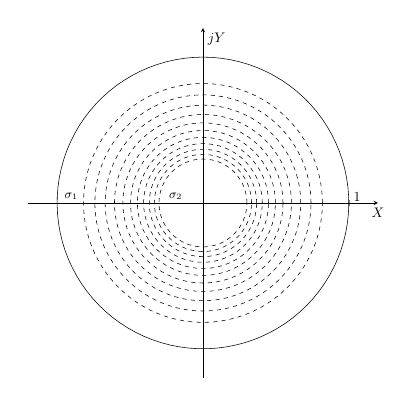
\begin{tikzpicture}[scale = 0.5]
  \begin{axis}[%
    axis lines=center,
    width=3.5in,
    height=3.5in,
    scale only axis,
    xmin=-1.2,
    xmax=1.2,
    ymin=-1.2,
    ymax=1.2,
    xtick={1},
    ytick=\empty,
    xticklabel style={anchor=south west, draw=none},
    xlabel={$X$},
    ylabel={$jY$},
    x label style={anchor=north}
  ]
  \addplot [color=black, forget plot]
    table[row sep=crcr]{%
  0	1\\
  0.0634239196565645	0.997986676471884\\
  0.126592453573749	0.991954812830795\\
  0.18925124436041	0.981928697262707\\
  0.251147987181079	0.967948701396356\\
  0.312033445698487	0.950071117740945\\
  0.371662455660328	0.928367933016073\\
  0.429794912089172	0.902926538286621\\
  0.486196736100469	0.873849377069785\\
  0.540640817455598	0.841253532831181\\
  0.59290792905464	0.805270257531059\\
  0.642787609686539	0.766044443118978\\
  0.690079011482112	0.72373403810507\\
  0.734591708657533	0.678509411557132\\
  0.776146464291757	0.630552667084523\\
  0.814575952050336	0.580056909571198\\
  0.849725429949514	0.527225467610502\\
  0.881453363447582	0.472271074772683\\
  0.909631995354518	0.415415013001886\\
  0.934147860265107	0.356886221591872\\
  0.954902241444074	0.296920375328275\\
  0.971811568323542	0.235758935509427\\
  0.984807753012208	0.173648177666931\\
  0.993838464461254	0.110838199901011\\
  0.998867339183008	0.0475819158237424\\
  0.999874127673875	-0.015865963834808\\
  0.996854775951942	-0.0792499568567885\\
  0.989821441880933	-0.142314838273285\\
  0.978802446214779	-0.204806668065191\\
  0.963842158559942	-0.266473813690035\\
  0.945000818714669	-0.327067963317421\\
  0.922354294104581	-0.386345125693128\\
  0.895993774291336	-0.444066612605774\\
  0.866025403784439	-0.5\\
  0.832569854634771	-0.55392006386611\\
  0.795761840530832	-0.605609687137666\\
  0.755749574354258	-0.654860733945285\\
  0.712694171378863	-0.701474887706321\\
  0.666769000516292	-0.745264449675755\\
  0.618158986220605	-0.786053094742787\\
  0.567059863862771	-0.823676581429833\\
  0.513677391573407	-0.857983413234977\\
  0.458226521727411	-0.888835448654923\\
  0.400930535406614	-0.916108457432069\\
  0.342020143325669	-0.939692620785908\\
  0.28173255684143	-0.959492973614497\\
  0.220310532786541	-0.975429786885407\\
  0.15800139597335	-0.987438888676394\\
  0.0950560433041829	-0.995471922573085\\
  0.0317279334980681	-0.999496542383185\\
  -0.0317279334980679	-0.999496542383185\\
  -0.0950560433041826	-0.995471922573085\\
  -0.15800139597335	-0.987438888676394\\
  -0.220310532786541	-0.975429786885407\\
  -0.281732556841429	-0.959492973614497\\
  -0.342020143325669	-0.939692620785908\\
  -0.400930535406613	-0.91610845743207\\
  -0.45822652172741	-0.888835448654924\\
  -0.513677391573406	-0.857983413234977\\
  -0.567059863862771	-0.823676581429833\\
  -0.618158986220605	-0.786053094742788\\
  -0.666769000516292	-0.745264449675755\\
  -0.712694171378863	-0.701474887706322\\
  -0.755749574354258	-0.654860733945285\\
  -0.795761840530832	-0.605609687137667\\
  -0.832569854634771	-0.55392006386611\\
  -0.866025403784438	-0.5\\
  -0.895993774291336	-0.444066612605774\\
  -0.922354294104581	-0.386345125693129\\
  -0.945000818714668	-0.327067963317422\\
  -0.963842158559942	-0.266473813690035\\
  -0.978802446214779	-0.204806668065191\\
  -0.989821441880933	-0.142314838273285\\
  -0.996854775951942	-0.0792499568567888\\
  -0.999874127673875	-0.0158659638348076\\
  -0.998867339183008	0.0475819158237424\\
  -0.993838464461254	0.110838199901011\\
  -0.984807753012208	0.17364817766693\\
  -0.971811568323542	0.235758935509427\\
  -0.954902241444074	0.296920375328275\\
  -0.934147860265107	0.356886221591872\\
  -0.909631995354519	0.415415013001886\\
  -0.881453363447582	0.472271074772682\\
  -0.849725429949514	0.527225467610502\\
  -0.814575952050336	0.580056909571198\\
  -0.776146464291757	0.630552667084522\\
  -0.734591708657534	0.678509411557132\\
  -0.690079011482113	0.723734038105069\\
  -0.64278760968654	0.766044443118977\\
  -0.59290792905464	0.805270257531059\\
  -0.540640817455597	0.841253532831181\\
  -0.486196736100469	0.873849377069785\\
  -0.429794912089172	0.902926538286621\\
  -0.371662455660328	0.928367933016072\\
  -0.312033445698487	0.950071117740945\\
  -0.251147987181079	0.967948701396356\\
  -0.189251244360411	0.981928697262707\\
  -0.12659245357375	0.991954812830795\\
  -0.0634239196565654	0.997986676471884\\
  -2.44929359829471e-16	1\\
  };
  \addplot [color=black, dashed, forget plot]
    table[row sep=crcr]{%
  0.818730753077982	0\\
  0.818689816881465	0.00818717107633658\\
  0.818567012385498	0.0163735234423881\\
  0.818362351870431	0.02455823846974\\
  0.818075855802142	0.0327404976937101\\
  0.817707552830001	0.0409194828951944\\
  0.817257479783998	0.0490943761824887\\
  0.816725681671062	0.0572643600730765\\
  0.816112211670561	0.0654286175753772\\
  0.815417131128984	0.073586332270444\\
  0.814640509553807	0.0817366883936055\\
  0.813782424606539	0.0898788709160414\\
  0.81284296209496	0.0980120656262844\\
  0.811822215964538	0.106135459211641\\
  0.810720288289036	0.114248239339523\\
  0.809537289260304	0.122349594738677\\
  0.808273337177257	0.130438715280315\\
  0.806928558434052	0.138514792059124\\
  0.805503087507441	0.146577017474155\\
  0.80399706694333	0.154624585309586\\
  0.80241064734252	0.162656690815339\\
  0.800743987345649	0.170672530787558\\
  0.798997253617328	0.178671303648924\\
  0.797170620829474	0.186652209528818\\
  0.795264271643844	0.194614450343302\\
  0.793278396693767	0.20255722987493\\
  0.791213194565084	0.210479753852367\\
  0.789068871776287	0.218381230029819\\
  0.786845642757867	0.226260868266251\\
  0.784543729830874	0.234117880604407\\
  0.782163363184683	0.241951481349599\\
  0.779704780853973	0.249760887148283\\
  0.77716822869493	0.257545317066385\\
  0.774553960360655	0.2653039926674\\
  0.771862237275804	0.273036138090235\\
  0.769093328610441	0.280740980126791\\
  0.766247511253127	0.288417748299283\\
  0.763325069783224	0.296065674937293\\
  0.760326296442446	0.30368399525453\\
  0.757251491105626	0.31127194742531\\
  0.754100961250737	0.318828772660741\\
  0.750875021928137	0.326353715284595\\
  0.747573995729073	0.333846022808881\\
  0.744198212753411	0.34130494600909\\
  0.740748010576637	0.348729738999119\\
  0.737223734216094	0.356119659305854\\
  0.73362573609648	0.363473967943424\\
  0.729954376014609	0.370791929487094\\
  0.72621002110343	0.378072812146808\\
  0.722393045795313	0.385315887840366\\
  0.71850383178461	0.392520432266236\\
  0.714542767989478	0.399685724975979\\
  0.710510250512999	0.406811049446294\\
  0.706406682603558	0.413895693150673\\
  0.702232474614527	0.420938947630648\\
  0.697988043963226	0.427940108566642\\
  0.693673815089183	0.434898475848395\\
  0.689290219411692	0.441813353644977\\
  0.684837695286665	0.448684050474371\\
  0.680316687962807	0.45550987927262\\
  0.67572764953708	0.462290157462532\\
  0.671071038909504	0.469024207021938\\
  0.666347321737262	0.475711354551494\\
  0.661556970388133	0.48235093134202\\
  0.656700463893262	0.488942273441369\\
  0.651778287899249	0.495484721720825\\
  0.646790934619593	0.501977621941011\\
  0.641738902785466	0.508420324817316\\
  0.636622697595841	0.514812186084822\\
  0.631442830666973	0.521152566562728\\
  0.62619981998124	0.527440832218271\\
  0.62089418983534	0.533676354230123\\
  0.615526470787866	0.539858509051282\\
  0.610097199606251	0.545986678471416\\
  0.604606919213087	0.552060249678691\\
  0.59905617863184	0.558078615321046\\
  0.593445532931941	0.564041173566933\\
  0.587775543173286	0.569947328165496\\
  0.582046776350124	0.575796488506197\\
  0.576259805334365	0.581588069677877\\
  0.570415208818287	0.587321492527244\\
  0.564513571256672	0.59299618371679\\
  0.558555482808358	0.598611575782127\\
  0.552541539277224	0.604167107188727\\
  0.546472342052612	0.60966222238808\\
  0.540348498049187	0.615096371873243\\
  0.534170619646246	0.620469012233798\\
  0.527939324626481	0.625779606210185\\
  0.521655236114201	0.631027622747433\\
  0.515318982513022	0.63621253704826\\
  0.508931197443021	0.641333830625558\\
  0.502492519677385	0.646390991354236\\
  0.496003593078523	0.651383513522436\\
  0.489465066533689	0.656310897882102\\
  0.482877593890087	0.661172651698904\\
  0.476241833889492	0.665968288801511\\
  0.469558450102376	0.670697329630209\\
  0.462828110861547	0.675359301284857\\
  0.45605148919532	0.679953737572175\\
  0.449229262760216	0.684480179052361\\
  0.442362113773192	0.68893817308504\\
  0.435450728943425	0.693327273874524\\
  0.428495799403637	0.697647042514391\\
  0.421498020640988	0.701897047031378\\
  0.414458092427522	0.706076862428573\\
  0.407376718750194	0.710186070727922\\
  0.40025460774047	0.714224261012017\\
  0.393092471603517	0.718191029465196\\
  0.385891026546979	0.722085979413918\\
  0.378650992709362	0.725908721366436\\
  0.371373094088015	0.729658873051739\\
  0.364058058466735	0.733336059457784\\
  0.35670661734299	0.736939912868994\\
  0.349319505854765	0.740470072903032\\
  0.341897462707053	0.743926186546837\\
  0.334441230097984	0.747307908191922\\
  0.326951553644605	0.750614899668944\\
  0.31942918230832	0.753846830281508\\
  0.311874868319995	0.757003376839248\\
  0.304289367104733	0.760084223690138\\
  0.296673437206333	0.763089062752061\\
  0.289027840211441	0.766017593543614\\
  0.281353340673382	0.768869523214158\\
  0.273650706035717	0.771644566573104\\
  0.26592070655549	0.774342446118427\\
  0.258164115226207	0.776962892064421\\
  0.250381707700537	0.779505642368676\\
  0.242574262212748	0.78197044275828\\
  0.234742559500882	0.784357046755248\\
  0.226887382728685	0.786665215701169\\
  0.219009517407286	0.788894718781072\\
  0.211109751316655	0.791045333046507\\
  0.203188874426816	0.79311684343784\\
  0.195247678818857	0.795109042805757\\
  0.187286958605723	0.797021731931983\\
  0.1793075098528	0.798854719549198\\
  0.171310130498314	0.800607822360168\\
  0.163295620273536	0.802280865056073\\
  0.15526478062281	0.803873680334037\\
  0.147218414623409	0.805386108913861\\
  0.139157326905227	0.806817999553946\\
  0.131082323570319	0.808169209066422\\
  0.122994212112288	0.809439602331463\\
  0.114893801335541	0.810629052310802\\
  0.106781901274405	0.811737440060431\\
  0.0986593231121264	0.812764654742501\\
  0.0905268790997522	0.813710593636397\\
  0.0823853824749068	0.81457516214902\\
  0.0742356473804682	0.815358273824239\\
  0.0660784887831544	0.816059850351537\\
  0.0579147223920275	0.816679821573849\\
  0.0497451645769235	0.817218125494567\\
  0.0415706322868159	0.817674708283749\\
  0.0333919429681218	0.818049524283495\\
  0.0252099144829574	0.818342536012519\\
  0.0170253650273528	0.818553714169892\\
  0.00883911304943331	0.818683037637973\\
  0.000651977167574757	0.818730493484524\\
  -0.00753522391145724	0.818696076964\\
  -0.0157216714743774	0.818579791518024\\
  -0.0239065468832515	0.818381648775043\\
  -0.0320890316573593	0.818101668549168\\
  -0.0402683075550422	0.817739878838186\\
  -0.0484435566555264	0.817296315820769\\
  -0.0566139614407145	0.816771023852847\\
  -0.0647787048769367	0.816164055463181\\
  -0.0729369704966532	0.815475471348102\\
  -0.0810879424801005	0.81470534036545\\
  -0.0892308057368731	0.813853739527679\\
  -0.0973647459874307	0.812920753994165\\
  -0.105488949844527	0.811906477062684\\
  -0.113602604894545	0.810811010160082\\
  -0.121704899778743	0.809634462832138\\
  -0.129795024274383	0.808376952732605\\
  -0.137872169375758	0.807038605611443\\
  -0.145935527375089	0.805619555302249\\
  -0.153984291943294	0.804119943708873\\
  -0.162017658210625	0.802539920791224\\
  -0.170034822847149	0.800879644550277\\
  -0.178034984143084	0.799139281012272\\
  -0.186017342088966	0.797319004212113\\
  -0.193981098455654	0.795418996175963\\
  -0.201925456874146	0.793439446903043\\
  -0.209849622915221	0.79138055434663\\
  -0.217752804168879	0.789242524394263\\
  -0.22563421032358	0.787025570847157\\
  -0.233493053245277	0.784729915398819\\
  -0.241328547056226	0.78235578761288\\
  -0.249139908213576	0.779903424900141\\
  -0.256926355587721	0.777373072494829\\
  -0.264687110540411	0.774764983430077\\
  -0.272421397002619	0.772079418512617\\
  -0.280128441552144	0.769316646296703\\
  -0.287807473490953	0.766476943057254\\
  -0.295457724922252	0.763560592762229\\
  -0.303078430827272	0.760567887044225\\
  -0.310668829141775	0.757499125171322\\
  -0.318228160832253	0.754354614017148\\
  -0.325755669971837	0.7511346680302\\
  -0.333250603815886	0.747839609202392\\
  -0.340712212877262	0.744469767036861\\
  -0.348139751001275	0.741025478515017\\
  -0.355532475440304	0.737507088062839\\
  -0.362889646928065	0.733914947516443\\
  -0.37021052975354	0.730249416086889\\
  -0.377494391834548	0.726510860324265\\
  -0.38474050479095	0.722699654081033\\
  -0.391948144017488	0.71881617847464\\
  -0.399116588756248	0.714860821849411\\
  -0.406245122168727	0.710833979737713\\
  -0.413333031407527	0.7067360548204\\
  -0.420379607687628	0.70256745688655\\
  -0.427384146357277	0.698328602792483\\
  -0.434345946968441	0.694019916420075\\
  -0.441264313346863	0.689641828634372\\
  -0.448138553661668	0.685194777240506\\
  -0.454967980494556	0.68067920693991\\
  -0.461751910908532	0.676095569285851\\
  -0.46848966651621	0.671444322638273\\
  -0.475180573547642	0.666725932117968\\
  -0.481823962917703	0.661940869560053\\
  -0.48841917029299	0.657089613466798\\
  -0.494965536158263	0.652172648959769\\
  -0.50146240588239	0.64719046773132\\
  -0.507909129783812	0.642143567995421\\
  -0.514305063195512	0.637032454437841\\
  -0.520649566529479	0.631857638165675\\
  -0.526942005340666	0.626619636656239\\
  -0.533181750390436	0.621318973705318\\
  -0.539368177709483	0.615956179374792\\
  -0.545500668660232	0.610531789939622\\
  -0.551578609998697	0.605046347834234\\
  -0.557601393935809	0.599500401598266\\
  -0.563568418198194	0.59389450582172\\
  -0.569479086088398	0.588229221089502\\
  -0.575332806544557	0.582505113925365\\
  -0.581128994199505	0.576722756735254\\
  -0.586867069439305	0.570882727750071\\
  -0.592546458461215	0.564985610967846\\
  -0.598166593331066	0.559031996095345\\
  -0.603726912040055	0.553022478489093\\
  -0.609226858560944	0.546957659095842\\
  -0.614665882903664	0.540838144392478\\
  -0.620043441170313	0.534664546325372\\
  -0.625358995609547	0.528437482249185\\
  -0.63061201467035	0.522157574865137\\
  -0.635801973055195	0.515825452158732\\
  -0.640928351772567	0.509441747336964\\
  -0.645990638188867	0.503007098764996\\
  -0.650988326079673	0.496522149902323\\
  -0.655920915680358	0.489987549238427\\
  -0.660787913736075	0.483403950227928\\
  -0.665588833551072	0.476772011225242\\
  -0.67032319503737	0.470092395418742\\
  -0.674990524762766	0.463365770764442\\
  -0.679590355998175	0.456592809919203\\
  -0.684122228764307	0.449774190173465\\
  -0.688585689877663	0.44291059338352\\
  -0.692980292995851	0.436002705903327\\
  -0.697305598662221	0.429051218515879\\
  -0.701561174349811	0.42205682636412\\
  -0.705746594504598	0.415020228881438\\
  -0.709861440588055	0.407942129721717\\
  -0.713905301119003	0.400823236688974\\
  -0.717877771714757	0.39366426166658\\
  -0.72177845513157	0.386465920546073\\
  -0.725606961304349	0.379228933155564\\
  -0.729362907385669	0.371954023187764\\
  -0.73304591778405	0.364641918127605\\
  -0.736655624201523	0.3572933491795\\
  -0.740191665670453	0.349909051194221\\
  -0.74365368858964	0.342489762595413\\
  -0.747041346759677	0.335036225305752\\
  -0.750354301417572	0.327549184672756\\
  -0.753592221270617	0.32002938939425\\
  -0.756754782529527	0.312477591443495\\
  -0.759841668940811	0.304894545993993\\
  -0.762852571818399	0.297281011343969\\
  -0.765787190074515	0.289637748840544\\
  -0.768645230249777	0.281965522803599\\
  -0.771426406542549	0.274265100449344\\
  -0.774130440837521	0.266537251813598\\
  -0.776757062733515	0.258782749674784\\
  -0.779306009570531	0.251002369476654\\
  -0.78177702645601	0.243196889250744\\
  -0.784169866290322	0.235367089538573\\
  -0.786484289791477	0.227513753313586\\
  -0.788720065519055	0.219637665902862\\
  -0.790876969897345	0.211739614908579\\
  -0.792954787237708	0.203820390129254\\
  -0.79495330976014	0.195880783480766\\
  -0.796872337614055	0.187921588917163\\
  -0.798711678898266	0.179943602351269\\
  -0.800471149680179	0.171947621575093\\
  -0.802150574014181	0.163934446180048\\
  -0.803749783959238	0.155904877476997\\
  -0.805268619595688	0.147859718416118\\
  -0.806706929041234	0.139799773506614\\
  -0.808064568466129	0.131725848736259\\
  -0.809341402107563	0.123638751490801\\
  -0.810537302283234	0.115539290473226\\
  -0.811652149404123	0.107428275622886\\
  -0.812685831986446	0.0993065180345072\\
  -0.813638246662806	0.0911748298770798\\
  -0.814509298192529	0.0830340243126439\\
  -0.815298899471189	0.0748849154149711\\
  -0.816006971539315	0.0667283180881611\\
  -0.816633443590291	0.0585650479851486\\
  -0.817178252977433	0.0503959214261421\\
  -0.817641345220257	0.0422217553169894\\
  -0.818022674009925	0.0340433670674893\\
  -0.818322201213874	0.0258615745096522\\
  -0.818539896879636	0.017677195815915\\
  -0.818675739237824	0.0094910494173275\\
  -0.818729714704315	0.00130395392170711\\
  -0.818701817881609	-0.00688327196821883\\
  -0.818592051559363	-0.0150698095366836\\
  -0.81840042671412	-0.0232548401367532\\
  -0.818126962508203	-0.0314375452721878\\
  -0.817771686287805	-0.0396171066792934\\
  -0.817334633580253	-0.0477927064087448\\
  -0.816815848090453	-0.0559635269073824\\
  -0.816215381696521	-0.0641287510999658\\
  -0.815533294444597	-0.0722875624708793\\
  -0.814769654542837	-0.0804391451457855\\
  -0.813924538354596	-0.0885826839732092\\
  -0.812998030390787	-0.0967173646060545\\
  -0.811990223301435	-0.104842373583036\\
  -0.810901217866409	-0.112956898410029\\
  -0.809731122985346	-0.12106012764131\\
  -0.808480055666757	-0.129151250960711\\
  -0.807148141016333	-0.137229459262641\\
  -0.805735512224429	-0.145293944733003\\
  -0.804242310552746	-0.153343900929968\\
  -0.802668685320207	-0.161378522864628\\
  -0.801014793888025	-0.169397007081482\\
  -0.799280801643964	-0.177398551738792\\
  -0.797466881985804	-0.185382356688759\\
  -0.795573216303999	-0.193347623557543\\
  -0.793599993963539	-0.201293555825093\\
  -0.791547412285014	-0.209219358904805\\
  -0.789415676524881	-0.217124240222975\\
  -0.787204999854939	-0.22500740929806\\
  -0.784915603341014	-0.23286807781972\\
  -0.782547715920849	-0.240705459727654\\
  -0.780101574381213	-0.248518771290202\\
  -0.777577423334221	-0.25630723118272\\
  -0.774975515192875	-0.264070060565708\\
  -0.772296110145821	-0.271806483162697\\
  -0.769539476131329	-0.279515725337875\\
  -0.766705888810506	-0.287197016173448\\
  -0.763795631539721	-0.294849587546733\\
  -0.760808995342276	-0.302472674206971\\
  -0.757746278879302	-0.310065513851848\\
  -0.754607788419893	-0.317627347203727\\
  -0.75139383781048	-0.325157418085574\\
  -0.748104748443446	-0.332654973496577\\
  -0.744740849224985	-0.340119263687441\\
  -0.741302476542218	-0.347549542235368\\
  -0.737789974229546	-0.354945066118695\\
  -0.734203693534275	-0.362305095791197\\
  -0.730543993081484	-0.36962889525604\\
  -0.726811238838169	-0.37691573213938\\
  -0.723005804076645	-0.384164877763602\\
  -0.719128069337216	-0.391375607220183\\
  -0.715178422390125	-0.398547199442188\\
  -0.711157258196775	-0.40567893727637\\
  -0.707064978870234	-0.412770107554889\\
  -0.702901993635025	-0.419820001166627\\
  -0.698668718786202	-0.426827913128097\\
  -0.694365577647723	-0.433793142653942\\
  -0.689993000530114	-0.440714993227016\\
  -0.685551424687446	-0.447592772668028\\
  -0.681041294273599	-0.454425793204766\\
  -0.676463060297857	-0.46121337154087\\
  -0.671817180579803	-0.467954828924163\\
  -0.667104119703537	-0.474649491214526\\
  -0.662324348971219	-0.481296688951306\\
  -0.657478346355938	-0.487895757420271\\
  -0.652566596453919	-0.494446036720072\\
  -0.647589590436058	-0.500946871828238\\
  -0.64254782599881	-0.507397612666676\\
  -0.637441807314417	-0.513797614166677\\
  -0.632272044980492	-0.520146236333424\\
  -0.62703905596896	-0.526442844309992\\
  -0.621743363574363	-0.53268680844083\\
  -0.616385497361525	-0.538877504334728\\
  -0.610965993112605	-0.545014312927255\\
  -0.605485392773509	-0.551096620542667\\
  -0.599944244399706	-0.55712381895527\\
  -0.594343102101415	-0.563095305450246\\
  -0.588682525988198	-0.569010482883922\\
  -0.582963082112949	-0.574868759743483\\
  -0.57718534241529	-0.580669550206125\\
  -0.571349884664376	-0.586412274197636\\
  -0.565457292401118	-0.592096357450403\\
  -0.559508154879833	-0.597721231560837\\
  -0.553503067009316	-0.603286334046214\\
  -0.547442629293349	-0.608791108400923\\
  -0.541327447770652	-0.614235004152117\\
  -0.535158133954284	-0.619617476914756\\
  -0.528935304770484	-0.62493798844605\\
  -0.522659582496984	-0.630196006699279\\
  -0.516331594700783	-0.635391005877\\
  -0.509951974175387	-0.640522466483624\\
  -0.503521358877532	-0.645589875377366\\
  -0.497040391863389	-0.650592725821561\\
  -0.490509721224258	-0.655530517535332\\
  -0.483930000021762	-0.660402756743623\\
  -0.477301886222538	-0.665208956226573\\
  -0.470626042632441	-0.66994863536824\\
  -0.463903136830268	-0.674621320204659\\
  -0.457133841100997	-0.67922654347124\\
  -0.450318832368558	-0.683763844649494\\
  -0.443458792128148	-0.688232770013084\\
  -0.436554406378073	-0.692632872673199\\
  -0.429606365551155	-0.696963712623238\\
  -0.422615364445685	-0.701224856782816\\
  -0.415582102155949	-0.705415879041067\\
  -0.408507282002314	-0.70953636029926\\
  -0.401391611460901	-0.713585888512701\\
  -0.394235802092833	-0.717564058731943\\
  -0.387040569473085	-0.72147047314328\\
  -0.379806633118923	-0.725304741108527\\
  -0.372534716417953	-0.729066479204081\\
  -0.365225546555786	-0.732755311259268\\
  -0.357879854443317	-0.736370868393956\\
  -0.350498374643636	-0.739912789055446\\
  -0.343081845298571	-0.743380719054622\\
  -0.335631008054877	-0.746774311601374\\
  -0.328146607990069	-0.750093227339276\\
  -0.320629393537917	-0.75333713437952\\
  -0.313080116413602	-0.756505708334104\\
  -0.305499531538544	-0.759598632348275\\
  -0.297888396964915	-0.762615597132207\\
  -0.290247473799828	-0.765556300991937\\
  -0.282577526129233	-0.76842044985953\\
  -0.274879320941507	-0.771207757322484\\
  -0.267153628050751	-0.773917944652377\\
  -0.259401220019817	-0.776550740832735\\
  -0.251622872083049	-0.779105882586133\\
  -0.243819362068757	-0.781583114400525\\
  -0.235991470321441	-0.783982188554794\\
  -0.228139979623751	-0.786302865143523\\
  -0.220265675118214	-0.788544912100989\\
  -0.212369344228721	-0.790708105224363\\
  -0.204451776581778	-0.792792228196136\\
  -0.196513763927552	-0.794797072605747\\
  -0.188556100060696	-0.796722437970427\\
  -0.180579580740962	-0.798568131755242\\
  -0.172585003613637	-0.800333969392353\\
  -0.164573168129772	-0.802019774299468\\
  -0.156544875466236	-0.8036253778975\\
  -0.148500928445608	-0.805150619627428\\
  -0.140442131455886	-0.80659534696635\\
  -0.132369290370052	-0.807959415442736\\
  -0.124283212465489	-0.809242688650875\\
  -0.116184706343249	-0.810445038264516\\
  -0.108074581847194	-0.811566344049698\\
  -0.0999536499830172	-0.812606493876779\\
  -0.0918227228371354	-0.813565383731642\\
  -0.0836826134954893	-0.814442917726101\\
  -0.0755341359622289	-0.815239008107487\\
  -0.0673781050783172	-0.815953575267426\\
  -0.0592153364400452	-0.816586547749797\\
  -0.0510466463174758	-0.81713786225788\\
  -0.0428728515728135	-0.817607463660683\\
  -0.0346947695787211	-0.817995304998457\\
  -0.026513218136583	-0.818301347487392\\
  -0.0183290153947248	-0.818525560523493\\
  -0.0101429797666021	-0.818667921685645\\
  -0.00195592984895508	-0.818728416737849\\
  0.00623131566004759	-0.818707039630651\\
  0.0144179380426763	-0.818603792501743\\
  0.0226031186435156	-0.818418685675753\\
  0.0307860389513265	-0.818151737663208\\
  0.0389658806808971	-0.817802975158688\\
  0.0471418258548719	-0.817372433038152\\
  0.0553130568855451	-0.816860154355454\\
  0.0634787566566239	-0.816266190338034\\
  0.0716381086049365	-0.815590600381801\\
  0.0797902968020862	-0.814833452045186\\
  0.0879345060360473	-0.813994821042392\\
  0.0960699218926833	-0.81307479123582\\
  0.104195730837188	-0.812073454627685\\
  0.112311120295439	-0.810990911350813\\
  0.120415278735253	-0.80982726965863\\
  0.128507395747538	-0.808582645914334\\
  0.136586662127338	-0.807257164579263\\
  0.144652269954748	-0.805850958200447\\
  0.152703412675704	-0.804364167397351\\
  0.160739285182646	-0.802796940847816\\
  0.168759083895018	-0.801149435273191\\
  0.176762006839633	-0.799421815422662\\
  0.184747253730865	-0.797614254056773\\
  0.19271402605068	-0.795726931930155\\
  0.200661527128484	-0.793760037773447\\
  0.208588962220793	-0.791713768274426\\
  0.216495538590703	-0.789588328058337\\
  0.224380465587166	-0.787383929667431\\
  0.232242954724053	-0.785100793539709\\
  0.240082219759004	-0.782739147986881\\
  0.247897476772047	-0.780299229171535\\
  0.255687944243992	-0.777781281083519\\
  0.263452843134586	-0.775185555515544\\
  0.27119139696041	-0.772512312038003\\
  0.27890283187253	-0.769761817973016\\
  0.28658637673388	-0.766934348367698\\
  0.294241263196379	-0.764030185966653\\
  0.301866725777758	-0.761049621183701\\
  0.309462001938115	-0.757992952072837\\
  0.317026332156161	-0.754860484298424\\
  0.324558960005179	-0.751652531104629\\
  0.332059132228662	-0.748369413284099\\
  0.339526098815638	-0.74501145914588\\
  0.346959113075669	-0.741579004482587\\
  0.354357431713524	-0.738072392536826\\
  0.361720314903504	-0.73449197396687\\
  0.369047026363427	-0.730838106811591\\
  0.376336833428252	-0.727111156454661\\
  0.383589007123347	-0.72331149558801\\
  0.390802822237386	-0.719439504174558\\
  0.39797755739487	-0.715495569410218\\
  0.40511249512826	-0.711480085685183\\
  0.41220692194973	-0.707393454544477\\
  0.41926012842251	-0.703236084647809\\
  0.42627140923183	-0.699008391728704\\
  0.433240063255452	-0.694710798552931\\
  0.44016539363378	-0.690343734876227\\
  0.447046707839549	-0.68590763740132\\
  0.453883317747071	-0.68140294973426\\
  0.460674539701053	-0.676830122340061\\
  0.467419694584959	-0.672189612497651\\
  0.474118107888922	-0.667481884254148\\
  0.480769109777193	-0.662707408378452\\
  0.487372035155127	-0.657866662314172\\
  0.493926223735686	-0.652960130131882\\
  0.500431020105475	-0.64798830248071\\
  0.506885773790279	-0.642951676539279\\
  0.513289839320107	-0.637850755965984\\
  0.519642576293743	-0.632686050848634\\
  0.525943349442784	-0.627458077653436\\
  0.532191528695165	-0.622167359173352\\
  0.538386489238168	-0.616814424475821\\
  0.544527611580902	-0.611399808849854\\
  0.550614281616248	-0.6059240537525\\
  0.556645890682277	-0.600387706754705\\
  0.562621835623107	-0.594791321486557\\
  0.568541518849225	-0.589135457581917\\
  0.574404348397242	-0.583420680622464\\
  0.580209737989087	-0.577647562081131\\
  0.585957107090639	-0.571816679264962\\
  0.59164588096978	-0.565928615257377\\
  0.597275490753859	-0.559983958859874\\
  0.60284537348659	-0.553983304533135\\
  0.608354972184343	-0.547927252337595\\
  0.613803735891838	-0.541816407873425\\
  0.619191119737245	-0.53565138221998\\
  0.62451658498667	-0.529432791874688\\
  0.629779599098024	-0.523161258691401\\
  0.634979635774284	-0.516837409818211\\
  0.640116175016113	-0.510461877634736\\
  0.64518870317387	-0.50403529968888\\
  0.650196712998964	-0.497558318633084\\
  0.655139703694588	-0.491031582160055\\
  0.66001718096579	-0.484455742938002\\
  0.664828657068908	-0.477831458545366\\
  0.66957365086034	-0.471159391405068\\
  0.674251687844664	-0.46444020871826\\
  0.678862300222077	-0.457674582397613\\
  0.683405026935185	-0.450863189000121\\
  0.687879413715101	-0.444006709659447\\
  0.692285013126877	-0.43710583001781\\
  0.696621384614243	-0.430161240157426\\
  0.700888094543663	-0.423173634531493\\
  0.705084716247699	-0.41614371189475\\
  0.70921083006768	-0.409072175233603\\
  0.713266023395662	-0.401959731695824\\
  0.71724989071569	-0.394807092519841\\
  0.721162033644352	-0.387614972963612\\
  0.725002060970617	-0.380384092233097\\
  0.728769588694951	-0.373115173410344\\
  0.732464240067721	-0.365808943381179\\
  0.73608564562687	-0.358466132762516\\
  0.739633443234858	-0.351087475829297\\
  0.743107278114882	-0.343673710441067\\
  0.746506802886349	-0.336225577968187\\
  0.749831677599614	-0.328743823217697\\
  0.753081569769976	-0.321229194358838\\
  0.756256154410928	-0.313682442848232\\
  0.759355114066649	-0.306104323354743\\
  0.762378138843758	-0.298495593684005\\
  0.765324926442296	-0.290857014702644\\
  0.768195182185958	-0.283189350262192\\
  0.770988619051561	-0.275493367122705\\
  0.773704957697748	-0.267769834876083\\
  0.776343926492918	-0.260019525869113\\
  0.778905261542389	-0.252243215126239\\
  0.781388706714791	-0.244441680272054\\
  0.783794013667677	-0.236615701453543\\
  0.786120941872356	-0.228766061262066\\
  0.788369258637946	-0.2208935446551\\
  0.790538739134645	-0.212998938877746\\
  0.79262916641621	-0.205083033384003\\
  0.794640331441655	-0.197146619757823\\
  0.796572033096155	-0.189190491633956\\
  0.798424078211152	-0.181215444618583\\
  0.80019628158368	-0.173222276209761\\
  0.801888465994878	-0.16521178571767\\
  0.803500462227714	-0.157184774184683\\
  0.805032109083909	-0.149142044305263\\
  0.806483253400053	-0.141084400345699\\
  0.807853750062924	-0.13301264806367\\
  0.809143462023998	-0.124927594627678\\
  0.810352260313154	-0.116830048536328\\
  0.81148002405157	-0.108720819537484\\
  0.812526640463812	-0.100600718547286\\
  0.813492004889111	-0.0924705575690671\\
  0.814376020791828	-0.0843311496121492\\
  0.815178599771111	-0.0761833086105465\\
  0.81589966156973	-0.0680278493415686\\
  0.816539134082106	-0.0598655873443463\\
  0.817096953361521	-0.0516973388382766\\
  0.817573063626512	-0.0435239206414048\\
  0.817967417266448	-0.0353461500887386\\
  0.818279974846295	-0.0271648449505186\\
  0.818510705110555	-0.0189808233504402\\
  0.818659584986395	-0.0107949036838447\\
  0.818726599585949	-0.00260790453587651\\
  };
  \addplot [color=black, dashed, forget plot]
    table[row sep=crcr]{%
  0.740818220681718	0\\
  0.740781180079357	0.00740805873773108\\
  0.740670061976304	0.0148153766757617\\
  0.740484877484276	0.0222212130884709\\
  0.740225645121568	0.0296248273983889\\
  0.739892390811201	0.0370254792502543\\
  0.739485147878328	0.0444224285850491\\
  0.739003957046902	0.051814935714004\\
  0.738448866435607	0.0592022613925665\\
  0.737819931553039	0.0665836668943248\\
  0.737117215292165	0.0739584140848798\\
  0.736340787924023	0.0813257654956582\\
  0.735490727090705	0.0886849843976582\\
  0.734567117797584	0.0960353348751224\\
  0.73357005240482	0.103376081899128\\
  0.732499630618123	0.110706491401091\\
  0.731355959478778	0.118025830346168\\
  0.730139153352946	0.125333366806565\\
  0.728849333920227	0.132628370034726\\
  0.727486630161487	0.139910110536407\\
  0.726051178345969	0.147177860143625\\
  0.724543122017656	0.154430892087477\\
  0.722962611980926	0.161668481070812\\
  0.721309806285464	0.168889903340763\\
  0.719584870210464	0.176094436761121\\
  0.717787976248094	0.183281360884548\\
  0.715919304086254	0.19044995702462\\
  0.713979040590603	0.197599508327698\\
  0.711967379785874	0.204729299844609\\
  0.70988452283647	0.211838618602142\\
  0.707730678026351	0.218926753674347\\
  0.705506060738203	0.225992996253623\\
  0.7032108934319	0.2330366397216\\
  0.700845405622262	0.240056979719802\\
  0.698409833856097	0.247053314220078\\
  0.695904421688553	0.25402494359481\\
  0.693329419658759	0.260971170686868\\
  0.690685085264771	0.267891300879334\\
  0.687971682937826	0.274784642164953\\
  0.685189484015895	0.281650505215343\\
  0.682338766716552	0.288488203449919\\
  0.67941981610915	0.295297053104555\\
  0.676432924086319	0.302076373299962\\
  0.673378389334772	0.308825486109768\\
  0.670256517305438	0.315543716628317\\
  0.667067620182919	0.322230393038155\\
  0.663812016854269	0.328884846677213\\
  0.660490032877109	0.335506412105674\\
  0.657102000447067	0.342094427172512\\
  0.653648258364564	0.34864823308171\\
  0.650129152000929	0.35516717445814\\
  0.646545033263867	0.361650599413095\\
  0.642896260562264	0.368097859609484\\
  0.639183198770351	0.374508310326658\\
  0.635406219191211	0.38088131052489\\
  0.631565699519655	0.387216222909469\\
  0.62766202380445	0.393512413994436\\
  0.623695582409915	0.399769254165929\\
  0.619666771976883	0.405986117745146\\
  0.615575995383041	0.412162383050909\\
  0.611423661702639	0.418297432461834\\
  0.607210186165585	0.424390652478093\\
  0.602935990115921	0.430441433782763\\
  0.59860150096969	0.436449171302753\\
  0.594207152172196	0.44241326426932\\
  0.589753383154655	0.448333116278137\\
  0.585240639290258	0.454208135348935\\
  0.580669371849631	0.460037733984704\\
  0.576040037955708	0.465821329230439\\
  0.571353100538022	0.471558342731433\\
  0.566609028286408	0.477248200791118\\
  0.561808295604138	0.482890334428429\\
  0.556951382560479	0.488484179434705\\
  0.552038774842689	0.494029176430106\\
  0.547070963707446	0.499524770919554\\
  0.542048445931723	0.504970413348179\\
  0.536971723763112	0.510365559156276\\
  0.5318413048696	0.515709668833761\\
  0.5266577022888	0.52100220797412\\
  0.521421434376652	0.526242647327848\\
  0.516133024755582	0.531430462855377\\
  0.510793002262146	0.536565135779478\\
  0.505401900894143	0.541646152637137\\
  0.499960259757218	0.546673005330903\\
  0.494468623010949	0.551645191179695\\
  0.488927539814435	0.556562212969072\\
  0.483337564271378	0.561423579000952\\
  0.477699255374673	0.566228803142783\\
  0.472013176950513	0.570977404876156\\
  0.466279897602	0.575668909344855\\
  0.460499990652293	0.580302847402341\\
  0.454674034087269	0.584878755658671\\
  0.44880261049773	0.589396176526833\\
  0.442886307021142	0.593854658268504\\
  0.436925715282923	0.598253755039225\\
  0.430921431337279	0.602593026932985\\
  0.424874055607601	0.606872040026211\\
  0.418784192826423	0.61109036642116\\
  0.412652451974948	0.615247584288707\\
  0.406479446222151	0.619343277910529\\
  0.400265792863465	0.623377037720679\\
  0.394012113259045	0.627348460346535\\
  0.387719032771642	0.631257148649145\\
  0.381387180704059	0.635102711762936\\
  0.375017190236228	0.638884765134802\\
  0.368609698361887	0.642602930562556\\
  0.362165345824883	0.646256836232754\\
  0.3556847770551	0.649846116757875\\
  0.349168640104015	0.653370413212857\\
  0.342617586579892	0.656829373170991\\
  0.336032271582625	0.660222650739164\\
  0.329413353638225	0.663549906592446\\
  0.322761494632972	0.666810808008026\\
  0.316077359747223	0.670005028898479\\
  0.309361617388895	0.673132249844377\\
  0.30261493912663	0.676192158126233\\
  0.29583799962263	0.679184447755768\\
  0.289031476565198	0.682108819506512\\
  0.282196050600969	0.684964980943728\\
  0.275332405266843	0.687752646453652\\
  0.268441226921632	0.690471537272055\\
  0.26152320467743	0.693121381512123\\
  0.254579030330695	0.695701914191638\\
  0.247609398293076	0.698212877259484\\
  0.240615005521967	0.700654019621446\\
  0.233596551450819	0.703025097165323\\
  0.226554737919188	0.705325872785335\\
  0.219490269102561	0.707556116405838\\
  0.212403851441931	0.709715605004329\\
  0.20529619357316	0.711804122633747\\
  0.198168006256111	0.71382146044407\\
  0.191020002303575	0.715767416703197\\
  0.183852896509993	0.717641796817125\\
  0.176667405579969	0.719444413349405\\
  0.16946424805661	0.721175086039884\\
  0.162244144249665	0.722833641822737\\
  0.155007816163498	0.724419914843766\\
  0.147755987424887	0.725933746476993\\
  0.140489383210663	0.727374985340514\\
  0.133208730175193	0.728743487311646\\
  0.125914756377712	0.73003911554133\\
  0.118608191209521	0.731261740467825\\
  0.11128976532105	0.732411239829655\\
  0.103960210548788	0.733487498677842\\
  0.0966202598421036	0.7344904093874\\
  0.0892706471899519	0.735419871668092\\
  0.0819121075474733	0.736275792574466\\
  0.0745453767624997	0.737058086515142\\
  0.0671711915019708	0.737766675261381\\
  0.0597902891782675	0.738401487954897\\
  0.0524034078754715	0.73896246111495\\
  0.0450112862755573	0.739449538644691\\
  0.0376146635845248	0.739862671836774\\
  0.0302142794584793	0.740201819378223\\
  0.0228108739296665	0.740466947354567\\
  0.0154051873324696	0.74065802925323\\
  0.00799796022937719	0.74077504596618\\
  0.000589933336926741	0.740817985791844\\
  -0.00681815254836579	0.740786844436275\\
  -0.0142255566240853	0.740681625013582\\
  -0.0216315381559969	0.740502338045621\\
  -0.0290353565521192	0.740249001460939\\
  -0.0364362714367823	0.739921640592983\\
  -0.0438335427246652	0.739520288177567\\
  -0.0512264306948035	0.739044984349598\\
  -0.0586141960645608	0.738495776639062\\
  -0.0659961000635567	0.737872719966274\\
  -0.0733714045075426	0.737175876636381\\
  -0.0807393718722205	0.736405316333136\\
  -0.0880992653669939	0.735561116111926\\
  -0.0954503490086463	0.734643360392071\\
  -0.10279188769494	0.733652140948377\\
  -0.110123147278123	0.732587556901963\\
  -0.117443394638348	0.731449714710347\\
  -0.124751897756977	0.730238728156799\\
  -0.132047925789791	0.728954718338965\\
  -0.139330749140066	0.727597813656758\\
  -0.146599639531534	0.726168149799515\\
  -0.153853870081216	0.72466586973243\\
  -0.161092715372101	0.723091123682257\\
  -0.168315451525692	0.721444069122291\\
  -0.175521356274393	0.719724870756613\\
  -0.182709709033734	0.717933700503629\\
  -0.189879790974428	0.716070737478871\\
  -0.197030885094259	0.714136167977088\\
  -0.204162276289771	0.712130185453619\\
  -0.211273251427789	0.710052990505044\\
  -0.218363099416725	0.707904790849128\\
  -0.225431111277688	0.705685801304046\\
  -0.232476580215382	0.703396243766902\\
  -0.239498801688784	0.701036347191544\\
  -0.246497073481599	0.698606347565661\\
  -0.253470695772479	0.696106487887192\\
  -0.260418971205007	0.693537018140021\\
  -0.267341204957429	0.690898195268982\\
  -0.274236704812139	0.688190283154162\\
  -0.281104781224898	0.685413552584517\\
  -0.287944747393788	0.682568281230789\\
  -0.294755919327891	0.679654753617744\\
  -0.301537615915691	0.676673261095713\\
  -0.30828915899318	0.673624101811466\\
  -0.315009873411676	0.670507580678389\\
  -0.321699087105338	0.667324009345999\\
  -0.328356131158372	0.664073706168775\\
  -0.334980339871918	0.660756996174328\\
  -0.341571050830627	0.657374211030892\\
  -0.348127604968895	0.653925689014163\\
  -0.354649346636771	0.650411774973469\\
  -0.361135623665523	0.646832820297285\\
  -0.367585787432854	0.643189182878098\\
  -0.373999192927763	0.639481227076611\\
  -0.380375198815043	0.635709323685317\\
  -0.386713167499421	0.631873849891409\\
  -0.393012465189308	0.627975189239073\\
  -0.399272461960186	0.624013731591123\\
  -0.405492531817593	0.619989873090024\\
  -0.411672052759729	0.615904016118273\\
  -0.417810406839647	0.611756569258161\\
  -0.423906980227055	0.607547947250919\\
  -0.429961163269695	0.60327857095524\\
  -0.435972350554308	0.598948867305196\\
  -0.441939940967175	0.594559269267544\\
  -0.447863337754227	0.59011021579843\\
  -0.453741948580722	0.585602151799493\\
  -0.459575185590476	0.581035528073375\\
  -0.465362465464648	0.576410801278646\\
  -0.471103209480075	0.571728433884129\\
  -0.476796843567139	0.566988894122662\\
  -0.482442798367176	0.562192655944272\\
  -0.48804050928941	0.557340198968781\\
  -0.493589416567414	0.552432008437841\\
  -0.499088965315084	0.547468575166415\\
  -0.504538605582129	0.542450395493696\\
  -0.509937792409064	0.537377971233467\\
  -0.515285985881704	0.532251809623929\\
  -0.52058265118516	0.527072423276969\\
  -0.525827258657314	0.521840330126908\\
  -0.531019283841791	0.5165560533787\\
  -0.536158207540398	0.511220121455615\\
  -0.541243515865048	0.505833067946401\\
  -0.546274700289146	0.500395431551918\\
  -0.551251257698443	0.494907756031274\\
  -0.556172690441345	0.489370590147449\\
  -0.561038506378678	0.483784487612417\\
  -0.565848218932903	0.478150007031776\\
  -0.570601347136774	0.472467711848889\\
  -0.575297415681431	0.466738170288539\\
  -0.579935954963933	0.460961955300106\\
  -0.584516501134217	0.455139644500278\\
  -0.589038596141482	0.449271820115282\\
  -0.593501787779998	0.443359068922666\\
  -0.597905629734318	0.437401982192622\\
  -0.602249681623918	0.431401155628859\\
  -0.606533509047229	0.425357189309034\\
  -0.610756683625078	0.41927068762474\\
  -0.614918783043527	0.413142259221075\\
  -0.619019391096102	0.406972516935772\\
  -0.623058097725415	0.400762077737919\\
  -0.627034499064169	0.394511562666258\\
  -0.630948197475543	0.38822159676709\\
  -0.634798801592959	0.381892809031762\\
  -0.638585926359212	0.375525832333773\\
  -0.642309193064983	0.369121303365489\\
  -0.645968229386703	0.362679862574468\\
  -0.649562669423789	0.356202154099421\\
  -0.653092153735233	0.349688825705799\\
  -0.656556329375546	0.343140528721012\\
  -0.659954849930049	0.336557917969304\\
  -0.66328737554952	0.329941651706261\\
  -0.666553572984174	0.323292391553\\
  -0.669753115616989	0.316610802429991\\
  -0.672885683496367	0.309897552490582\\
  -0.675950963368133	0.30315331305417\\
  -0.678948648706851	0.296378758539081\\
  -0.681878439746489	0.289574566395118\\
  -0.684740043510381	0.282741417035828\\
  -0.687533173840537	0.27587999377045\\
  -0.690257551426252	0.268990982735596\\
  -0.692912903832037	0.262075072826625\\
  -0.695498965524864	0.255132955628768\\
  -0.698015477900719	0.248165325347957\\
  -0.700462189310461	0.241172878741416\\
  -0.702838855084989	0.234156315047977\\
  -0.705145237559706	0.227116335918163\\
  -0.707381106098286	0.220053645344021\\
  -0.709546237115738	0.212968949588721\\
  -0.711640414100765	0.205862957115936\\
  -0.713663427637414	0.198736378518991\\
  -0.715615075426017	0.191589926449807\\
  -0.717495162303421	0.184424315547636\\
  -0.719303500262505	0.177240262367597\\
  -0.721039908470981	0.170038485309021\\
  -0.722704213289474	0.162819704543612\\
  -0.724296248288889	0.155584641943431\\
  -0.725815854267054	0.14833402100871\\
  -0.727262879264637	0.141068566795498\\
  -0.728637178580344	0.133789005843164\\
  -0.729938614785388	0.126496066101736\\
  -0.731167057737234	0.119190476859112\\
  -0.73232238459261	0.111872968668126\\
  -0.733404479819794	0.1045442732735\\
  -0.734413235210163	0.0972051235386675\\
  -0.735348549889021	0.0898562533724849\\
  -0.736210330325678	0.0824983976558448\\
  -0.73699849034281	0.0751322921681878\\
  -0.73771295112507	0.0677586735139237\\
  -0.738353641226976	0.0603782790487739\\
  -0.738920496580053	0.052991846806034\\
  -0.739413460499237	0.0456001154227735\\
  -0.739832483688546	0.0382038240659707\\
  -0.740177524246012	0.0308037123585974\\
  -0.740448547667865	0.0234005203056582\\
  -0.74064552685199	0.0159949882201886\\
  -0.740768442100633	0.00858785664922631\\
  -0.74081728112237	0.00117986629975532\\
  -0.740792039033341	-0.00622824203536242\\
  -0.740692718357733	-0.0136357275514665\\
  -0.740519329027532	-0.0210418495061788\\
  -0.740271888381525	-0.028445867293475\\
  -0.73995042116357	-0.035847040517747\\
  -0.739554959520123	-0.0432446290678393\\
  -0.739085542997018	-0.0506378931910619\\
  -0.738542218535515	-0.0580260935671638\\
  -0.737925040467609	-0.0654084913822636\\
  -0.737234070510592	-0.0727843484027324\\
  -0.736469377760883	-0.080152927049014\\
  -0.73563103868712	-0.0875134904693849\\
  -0.734719137122513	-0.0948653026136362\\
  -0.733733764256457	-0.102207628306681\\
  -0.732675018625418	-0.109539733322067\\
  -0.731543006103077	-0.116860884455404\\
  -0.730337839889743	-0.124170349597679\\
  -0.729059640501033	-0.131467397808469\\
  -0.727708535755821	-0.138751299389035\\
  -0.726284660763454	-0.146021325955287\\
  -0.724788157910247	-0.153276750510627\\
  -0.723219176845237	-0.160516847518647\\
  -0.721577874465222	-0.167740892975678\\
  -0.719864414899074	-0.174948164483196\\
  -0.718078969491322	-0.182137941320055\\
  -0.716221716785017	-0.189309504514563\\
  -0.714292842503883	-0.196462136916376\\
  -0.712292539533741	-0.203595123268217\\
  -0.710221007903221	-0.210707750277392\\
  -0.708078454763759	-0.217799306687129\\
  -0.705865094368884	-0.224869083347696\\
  -0.703581148052791	-0.231916373287318\\
  -0.701226844208209	-0.238940471782875\\
  -0.698802418263559	-0.245940676430369\\
  -0.696308112659417	-0.252916287215171\\
  -0.693744176824263	-0.259866606582014\\
  -0.691110867149546	-0.266790939504754\\
  -0.688408446964037	-0.273688593555868\\
  -0.685637186507503	-0.2805588789757\\
  -0.682797362903682	-0.287401108741432\\
  -0.679889260132565	-0.29421459863579\\
  -0.676913169002008	-0.300998667315463\\
  -0.673869387118644	-0.307752636379236\\
  -0.670758218858123	-0.31447583043583\\
  -0.66757997533468	-0.321167577171443\\
  -0.664334974370018	-0.327827207416978\\
  -0.66102354046153	-0.334454055214959\\
  -0.657646004749846	-0.34104745788613\\
  -0.654202704985724	-0.347606756095717\\
  -0.650693985496271	-0.354131293919366\\
  -0.647120197150512	-0.360620418908732\\
  -0.643481697324302	-0.367073482156723\\
  -0.639778849864593	-0.373489838362391\\
  -0.636012025053044	-0.379868845895464\\
  -0.632181599568999	-0.386209866860504\\
  -0.628287956451813	-0.392512267160698\\
  -0.624331485062553	-0.398775416561269\\
  -0.620312581045062	-0.404998688752495\\
  -0.616231646286391	-0.411181461412343\\
  -0.612089088876617	-0.417323116268701\\
  -0.607885323068027	-0.423423039161199\\
  -0.6036207692337	-0.429480620102633\\
  -0.599295853825465	-0.435495253339956\\
  -0.59491100933126	-0.441466337414857\\
  -0.590466674231878	-0.447393275223903\\
  -0.585963292957128	-0.453275474078254\\
  -0.581401315841382	-0.459112345762925\\
  -0.576781199078553	-0.464903306595612\\
  -0.572103404676464	-0.470647777485057\\
  -0.567368400410659	-0.47634518398896\\
  -0.562576659777619	-0.481994956371416\\
  -0.557728661947413	-0.487596529659897\\
  -0.552824891715785	-0.49314934370174\\
  -0.547865839455671	-0.49865284322017\\
  -0.542852001068165	-0.50410647786982\\
  -0.537783877932927	-0.509509702291771\\
  -0.532661976858048	-0.514861976168082\\
  -0.527486810029366	-0.520162764275827\\
  -0.522258894959252	-0.525411536540612\\
  -0.516978754434857	-0.530607768089584\\
  -0.511646916465832	-0.535750939303919\\
  -0.506263914231532	-0.540840535870782\\
  -0.500830286027694	-0.545876048834756\\
  -0.49534657521261	-0.550856974648741\\
  -0.489813330152793	-0.555782815224308\\
  -0.484231104168136	-0.560653077981503\\
  -0.478600455476588	-0.56546727589811\\
  -0.472921947138324	-0.570224927558348\\
  -0.467196146999446	-0.574925557201016\\
  -0.461423627635198	-0.579568694767066\\
  -0.455604966292703	-0.584153875946613\\
  -0.44974074483325	-0.588680642225358\\
  -0.443831549674096	-0.593148540930446\\
  -0.437877971729833	-0.597557125275729\\
  -0.431880606353294	-0.601905954406448\\
  -0.425840053276019	-0.606194593443313\\
  -0.419756916548282	-0.610422613525994\\
  -0.413631804478686	-0.614589591856006\\
  -0.407465329573334	-0.618695111738989\\
  -0.401258108474579	-0.622738762626376\\
  -0.395010761899357	-0.626720140156447\\
  -0.388723914577119	-0.630638846194767\\
  -0.382398195187359	-0.634494488873998\\
  -0.376034236296745	-0.638286682633086\\
  -0.369632674295861	-0.642015048255815\\
  -0.363194149335574	-0.645679212908728\\
  -0.356719305263014	-0.649278810178415\\
  -0.350208789557194	-0.652813480108148\\
  -0.343663253264257	-0.656282869233879\\
  -0.337083350932379	-0.659686630619588\\
  -0.33046974054631	-0.663024423891972\\
  -0.323823083461576	-0.666295915274485\\
  -0.317144044338348	-0.669500777620715\\
  -0.310433291074972	-0.672638690447099\\
  -0.303691494741182	-0.675709339964968\\
  -0.296919329510992	-0.678712419111931\\
  -0.290117472595285	-0.681647627582573\\
  -0.283286604174081	-0.684514671858495\\
  -0.276427407328531	-0.687313265237659\\
  -0.269540567972604	-0.690043127863058\\
  -0.262626774784496	-0.692703986750704\\
  -0.255686719137764	-0.695295575816927\\
  -0.248721095032191	-0.697817635904979\\
  -0.241730599024381	-0.700269914810954\\
  -0.234715930158109	-0.702652167309003\\
  -0.227677789894418	-0.704964155175864\\
  -0.220616882041469	-0.707205647214675\\
  -0.213533912684162	-0.7093764192781\\
  -0.206429590113531	-0.711476254290743\\
  -0.199304624755913	-0.713504942270851\\
  -0.192159729101906	-0.715462280351318\\
  -0.184995617635121	-0.717348072799967\\
  -0.177813006760735	-0.719162131039123\\
  -0.17061261473385	-0.720904273664476\\
  -0.163395161587668	-0.722574326463213\\
  -0.15616136906149	-0.724172122431447\\
  -0.14891196052854	-0.725697501790913\\
  -0.14164766092363	-0.727150312004946\\
  -0.134369196670667	-0.728530407793735\\
  -0.12707729561001	-0.729837651148851\\
  -0.11977268692569	-0.731071911347049\\
  -0.112456101072488	-0.732233064963336\\
  -0.105128269702891	-0.733320995883319\\
  -0.0977899255939313	-0.734335595314812\\
  -0.0904418025739033	-0.735276761798718\\
  -0.0830846354489851	-0.736144401219174\\
  -0.0757191599297597	-0.736938426812958\\
  -0.0683461125576403	-0.737658759178175\\
  -0.0609662306312201	-0.738305326282187\\
  -0.0535802521325411	-0.738878063468824\\
  -0.0461889156532996	-0.739376913464844\\
  -0.0387929603209835	-0.739801826385662\\
  -0.0313931257249625	-0.740152759740341\\
  -0.0239901518425299	-0.740429678435838\\
  -0.0165847789649042	-0.740632554780514\\
  -0.00917774762320319	-0.740761368486904\\
  -0.00176979851438798	-0.740816106673744\\
  0.00563832757280451	-0.740796763867262\\
  0.0130458898319376	-0.740703342001721\\
  0.0204521475129591	-0.740535850419232\\
  0.0278563599962727	-0.740294305868811\\
  0.0352577868668002	-0.739978732504713\\
  0.0426556879880231	-0.739589161884012\\
  0.0500493235759928	-0.739125632963444\\
  0.0574379542733126	-0.738588192095516\\
  0.0648208412230704	-0.737976893023867\\
  0.0721972461427225	-0.737291796877894\\
  0.0795664313979245	-0.736532972166641\\
  0.0869276600762918	-0.735700494771947\\
  0.094280196061091	-0.734794447940857\\
  0.101623304104851	-0.7338149222773\\
  0.108956249902886	-0.732762015733025\\
  0.116278300166728	-0.73163583359781\\
  0.12358872269745	-0.73043648848893\\
  0.130886786458894	-0.729164100339896\\
  0.138171761650764	-0.727818796388463\\
  0.145442919781611	-0.726400711163904\\
  0.152699533741682	-0.724909986473562\\
  0.159940877875628	-0.723346771388661\\
  0.167166228055071	-0.721711222229408\\
  0.174374861751012	-0.720003502549357\\
  0.18156605810609	-0.718223783119051\\
  0.188739098006662	-0.716372241908952\\
  0.195893264154716	-0.714449064071636\\
  0.203027841139598	-0.712454441923286\\
  0.210142115509555	-0.710388574924453\\
  0.217235375843079	-0.708251669660116\\
  0.224306912820048	-0.706043939819021\\
  0.231356019292656	-0.703765606172312\\
  0.238381990356131	-0.701416896551456\\
  0.245384123419222	-0.698998045825456\\
  0.252361718274457	-0.69650929587737\\
  0.259314077168165	-0.693950895580119\\
  0.266240504870251	-0.6913231007716\\
  0.273140308743716	-0.688626174229105\\
  0.280012798813923	-0.68586038564304\\
  0.286857287837591	-0.68302601158996\\
  0.293673091371523	-0.680123335504906\\
  0.300459527841044	-0.67715264765307\\
  0.307215918608164	-0.674114245100761\\
  0.313941588039435	-0.671008431685701\\
  0.320635863573519	-0.667835517986645\\
  0.327298075788441	-0.664595821292318\\
  0.333927558468532	-0.661289665569689\\
  0.340523648671049	-0.657917381431576\\
  0.347085686792467	-0.654479306103583\\
  0.353613016634442	-0.650975783390378\\
  0.360104985469432	-0.647407163641311\\
  0.36656094410596	-0.643773803715384\\
  0.372980246953544	-0.640076066945562\\
  0.379362252087249	-0.636314323102441\\
  0.385706321311879	-0.632488948357269\\
  0.392011820225799	-0.628600325244334\\
  0.398278118284372	-0.624648842622706\\
  0.404504588863013	-0.620634895637355\\
  0.410690609319855	-0.616558885679635\\
  0.416835561058005	-0.612421220347143\\
  0.422938829587411	-0.608222313402967\\
  0.428999804586307	-0.6039625847343\\
  0.435017879962242	-0.599642460310461\\
  0.440992453912696	-0.59526237214029\\
  0.44692292898525	-0.590822758228956\\
  0.45280871213734	-0.58632406253415\\
  0.458649214795555	-0.581766734921693\\
  0.464443852914499	-0.577151231120546\\
  0.470192047035185	-0.572478012677246\\
  0.475893222342993	-0.567747546909741\\
  0.481546808725143	-0.562960306860667\\
  0.487152240827709	-0.558116771250038\\
  0.492708958112151	-0.553217424427381\\
  0.498216404911371	-0.548262756323294\\
  0.503674030485278	-0.543253262400458\\
  0.509081289075865	-0.538189443604092\\
  0.514437639961776	-0.533071806311856\\
  0.519742547512388	-0.527900862283213\\
  0.524995481241366	-0.522677128608258\\
  0.530195915859714	-0.517401127656004\\
  0.535343331328306	-0.512073387022151\\
  0.540437212909882	-0.506694439476323\\
  0.54547705122053	-0.501264822908791\\
  0.550462342280619	-0.495785080276687\\
  0.555392587565197	-0.490255759549708\\
  0.560267294053844	-0.48467741365532\\
  0.565085974279973	-0.479050600423462\\
  0.569848146379578	-0.47337588253077\\
  0.574553334139417	-0.467653827444303\\
  0.579201067044634	-0.461885007364802\\
  0.583790880325813	-0.456069999169468\\
  0.588322315005451	-0.450209384354273\\
  0.592794917943855	-0.444303748975816\\
  0.597208241884458	-0.438353683592714\\
  0.601561845498545	-0.432359783206546\\
  0.605855293429381	-0.426322647202356\\
  0.610088156335753	-0.420242879288713\\
  0.614260010934897	-0.414121087437342\\
  0.618370440044828	-0.407957883822328\\
  0.622419032626062	-0.401753884758896\\
  0.626405383822714	-0.39550971064178\\
  0.630329095002986	-0.389225985883192\\
  0.634189773799031	-0.382903338850368\\
  0.637987034146186	-0.376542401802746\\
  0.641720496321579	-0.370143810828726\\
  0.645389786982107	-0.363708205782076\\
  0.648994539201759	-0.357236230217937\\
  0.652534392508317	-0.350728531328473\\
  0.656008992919402	-0.344185759878147\\
  0.659417992977868	-0.337608570138655\\
  0.662761051786548	-0.330997619823489\\
  0.666037835042349	-0.324353570022171\\
  0.669248015069675	-0.317677085134144\\
  0.6723912708532	-0.310968832802333\\
  0.675467288069963	-0.304229483846383\\
  0.678475759120806	-0.297459712195571\\
  0.681416383161132	-0.290660194821422\\
  0.684288866130988	-0.283831611670007\\
  0.687092920784468	-0.27697464559395\\
  0.689828266718446	-0.270089982284146\\
  0.692494630400607	-0.263178310201188\\
  0.695091745196805	-0.256240320506523\\
  0.697619351397725	-0.249276706993341\\
  0.700077196244852	-0.24228816601719\\
  0.70246503395575	-0.235275396426343\\
  0.704782625748639	-0.228239099491915\\
  0.707029739866269	-0.221179978837737\\
  0.709206151599102	-0.214098740369992\\
  0.711311643307779	-0.206996092206624\\
  0.713346004444882	-0.199872744606532\\
  0.715309031575995	-0.192729409898539\\
  0.717200528400038	-0.185566802410163\\
  0.719020305768906	-0.178385638396186\\
  0.720768181706379	-0.171186635967022\\
  0.72244398142632	-0.163970515016917\\
  0.724047537350153	-0.156737997151952\\
  0.725578689123621	-0.149489805617887\\
  0.727037283632824	-0.142226665227834\\
  0.728423175019527	-0.134949302289779\\
  0.729736224695744	-0.127658444533954\\
  0.730976301357604	-0.120354821040057\\
  0.732143280998472	-0.113039162164351\\
  0.733237046921358	-0.105712199466627\\
  0.734257489750581	-0.0983746656370503\\
  0.735204507442708	-0.0910272944228885\\
  0.736078005296759	-0.0836708205551403\\
  0.736877895963677	-0.0763059796750613\\
  0.737604099455061	-0.0689335082606036\\
  0.738256543151168	-0.0615541435527642\\
  0.738835161808171	-0.0541686234818645\\
  0.739339897564687	-0.0467776865937563\\
  0.739770699947562	-0.0393820719759707\\
  0.740127525876915	-0.0319825191838057\\
  0.740410339670452	-0.0245797681663744\\
  0.740619113047028	-0.0171745591926089\\
  0.740753825129479	-0.00976763277723687\\
  0.740814462446711	-0.00235972960672677\\
  };
  \addplot [color=black, dashed, forget plot]
    table[row sep=crcr]{%
  0.670320046035639	0\\
  0.670286530312637	0.00670308874090732\\
  0.670185986495173	0.0134055071785264\\
  0.670018424637546	0.0201065850765989\\
  0.669783861495802	0.0268056523329192\\
  0.669482320526061	0.0335020390463441\\
  0.669113831882166	0.0401950755837827\\
  0.668678432412676	0.0468840926471587\\
  0.668176165657176	0.0535684213403399\\
  0.667607081841921	0.0602473932360272\\
  0.666971237874819	0.066920340442597\\
  0.666268697339737	0.0735865956708893\\
  0.665499530490144	0.0802454923009364\\
  0.664663814242082	0.0868963644486245\\
  0.663761632166481	0.0935385470322811\\
  0.662793074480797	0.100171375839183\\
  0.661758238039989	0.106794187591977\\
  0.660657226326842	0.113406320015006\\
  0.659490149441607	0.120007111900539\\
  0.658257124091001	0.126595903174888\\
  0.656958273576533	0.133172034964415\\
  0.65559372778217	0.139734849661422\\
  0.654163623161354	0.146283690989909\\
  0.652668102723358	0.152817904071199\\
  0.651107316018977	0.159336835489429\\
  0.649481419125582	0.165839833356891\\
  0.647790574631507	0.172326247379217\\
  0.646034951619793	0.17879542892041\\
  0.644214725651277	0.185246731067706\\
  0.642330078747041	0.191679508696267\\
  0.640381199370202	0.198093118533691\\
  0.638368282407076	0.204486919224338\\
  0.636291529147681	0.210860271393469\\
  0.634151147265613	0.217212537711176\\
  0.631947350797275	0.223543082956122\\
  0.629680360120478	0.229851274079058\\
  0.627350401932402	0.236136480266128\\
  0.624957709226922	0.242398073001951\\
  0.622502521271317	0.248635426132471\\
  0.619985083582334	0.254847915927574\\
  0.617405647901646	0.261034921143457\\
  0.61476447217067	0.267195823084754\\
  0.61206182050478	0.273330005666404\\
  0.609297963166888	0.279436855475262\\
  0.606473176540427	0.285515761831436\\
  0.603587743101704	0.291566116849356\\
  0.60064195139166	0.297587315498562\\
  0.597636095987009	0.303578755664207\\
  0.594570477470788	0.309539838207266\\
  0.591445402402294	0.315469967024454\\
  0.588261183286429	0.321368549107831\\
  0.585018138542451	0.327234994604102\\
  0.581716592472133	0.333068716873608\\
  0.57835687522733	0.338869132548984\\
  0.574939322776966	0.344635661593494\\
  0.571464276873439	0.35036772735904\\
  0.567932085018444	0.356064756643823\\
  0.564343100428222	0.361726179749661\\
  0.560697681998241	0.367351430538961\\
  0.556996194267307	0.372939946491333\\
  0.553239007381108	0.378491168759837\\
  0.549426497055202	0.384004542226874\\
  0.545559044537445	0.389479515559691\\
  0.541637036569865	0.394915541265518\\
  0.53766086534999	0.400312075746313\\
  0.53363092849163	0.405668579353125\\
  0.529547628985111	0.410984516440058\\
  0.525411375156982	0.416259355417834\\
  0.521222580629179	0.421492568806949\\
  0.516981664277664	0.426683633290426\\
  0.512689050190537	0.431832029766142\\
  0.508345167625631	0.436937243398741\\
  0.503950450967582	0.441998763671113\\
  0.499505339684394	0.447016084435449\\
  0.49501027828349	0.451988703963853\\
  0.490465716267264	0.456916124998517\\
  0.485872108088133	0.461797854801444\\
  0.481229913103084	0.466633405203721\\
  0.476539595527749	0.471422292654337\\
  0.471801624389976	0.476164038268538\\
  0.467016473482931	0.480858167875714\\
  0.462184621317716	0.485504212066817\\
  0.457306551075523	0.490101706241299\\
  0.452382750559309	0.494650190653573\\
  0.447413712145024	0.499149210458989\\
  0.442399932732367	0.503598315759315\\
  0.437341913695103	0.507997061647729\\
  0.43224016083092	0.512345008253308\\
  0.427095184310853	0.516641720785014\\
  0.421907498628266	0.520886769575175\\
  0.416677622547404	0.52507973012245\\
  0.411406079051518	0.529220183134277\\
  0.406093395290564	0.533307714568806\\
  0.400740102528491	0.5373419156763\\
  0.395346736090115	0.54132238304001\\
  0.389913835307583	0.545248718616516\\
  0.384441943466448	0.549120529775533\\
  0.378931607751334	0.552937429339171\\
  0.37338337919122	0.556699035620655\\
  0.367797812604338	0.560404972462491\\
  0.362175466542694	0.564054869274084\\
  0.356516903236206	0.567648361068793\\
  0.350822688536492	0.571185088500435\\
  0.345093391860275	0.574664697899212\\
  0.339329586132449	0.578086841307085\\
  0.333531847728784	0.581451176512564\\
  0.327700756418288	0.584757367084934\\
  0.321836895305233	0.588005082407891\\
  0.315940850770844	0.591193997712609\\
  0.310013212414661	0.594323794110217\\
  0.30405457299558	0.597394158623682\\
  0.298065528372578	0.600404784219111\\
  0.292046677445126	0.603355369836454\\
  0.2859986220933	0.606245620419608\\
  0.279921967117596	0.609075246945923\\
  0.273817320178449	0.611843966455104\\
  0.267685291735464	0.614551502077508\\
  0.261526494986375	0.617197583061829\\
  0.255341545805726	0.619781944802173\\
  0.24913106268328	0.62230432886452\\
  0.242895666662175	0.624764483012566\\
  0.236635981276815	0.627162161232946\\
  0.230352632490524	0.629497123759837\\
  0.224046248632944	0.63176913709893\\
  0.217717460337205	0.633977974050786\\
  0.211366900476863	0.63612341373355\\
  0.204995204102612	0.638205241605042\\
  0.198603008378779	0.640223249484209\\
  0.19219095251961	0.642177235571946\\
  0.185759677725348	0.644067004471271\\
  0.179309827118113	0.64589236720687\\
  0.17284204567759	0.64765314124399\\
  0.166356980176534	0.649349150506695\\
  0.159855279116091	0.650980225395471\\
  0.153337592660948	0.65254620280419\\
  0.14680457257432	0.654046926136415\\
  0.140256872152772	0.655482245321063\\
  0.133695146160888	0.656852016827413\\
  0.127120050765801	0.658156103679455\\
  0.12053224347157	0.659394375469591\\
  0.113932383053436	0.660566708371673\\
  0.107321129491939	0.661672985153388\\
  0.100699143906927	0.662713095187981\\
  0.0940670884914398	0.663686934465313\\
  0.0874256264454925	0.66459440560227\\
  0.0807754219097552	0.665435417852493\\
  0.0741171398991396	0.666209887115459\\
  0.067451446236298	0.666917735944887\\
  0.0607790074850423	0.667558893556482\\
  0.054100490883687	0.66813329583502\\
  0.0474165642783269	0.668640885340749\\
  0.0407278960560527	0.669081611315144\\
  0.0340351550781127	0.669455429685973\\
  0.0273390106130274	0.669762303071711\\
  0.0206401322696632	0.670002200785275\\
  0.0139391899302721	0.670175098837095\\
  0.00723685368350395	0.670280979937507\\
  0.00053379375739813	0.670319833498492\\
  -0.0061693195476386	0.670291655634725\\
  -0.0128718159258617	0.670196449163969\\
  -0.0195730251332186	0.670034223606792\\
  -0.026272277054373	0.669804995185614\\
  -0.0329689017697155	0.669508786823086\\
  -0.039662229622355	0.669145628139798\\
  -0.046351591285084	0.668715555451316\\
  -0.0530363178273107	0.66821861176455\\
  -0.0597157407819514	0.667654846773454\\
  -0.0663891922122768	0.667024316854058\\
  -0.0730560047787052	0.666327085058829\\
  -0.0797155118055356	0.665563221110364\\
  -0.0863670473476147	0.664732801394422\\
  -0.0930099462569314	0.663835908952283\\
  -0.0996435442491305	0.662872633472444\\
  -0.106267177969941	0.66184307128165\\
  -0.112880185061509	0.660747325335261\\
  -0.119481904228639	0.65958550520696\\
  -0.126071675304913	0.65835772707779\\
  -0.132648839318716	0.657064113724543\\
  -0.139212738559128	0.655704794507475\\
  -0.145762716641694	0.654279905357375\\
  -0.152298118574064	0.65278958876197\\
  -0.158818290821491	0.651233993751679\\
  -0.165322581372185	0.649613275884706\\
  -0.17181033980251	0.647927597231487\\
  -0.178280917342029	0.646177126358483\\
  -0.184733666938381	0.644362038311322\\
  -0.191167943321983	0.642482514597296\\
  -0.197583103070559	0.640538743167211\\
  -0.20397850467348	0.63853091839659\\
  -0.210353508595916	0.636459241066236\\
  -0.216707477342786	0.634323918342157\\
  -0.22303977552251	0.632125163754845\\
  -0.229349769910548	0.629863197177927\\
  -0.235636829512719	0.627538244806175\\
  -0.241900325628302	0.62515053913289\\
  -0.248139631912906	0.622700318926648\\
  -0.2543541244411	0.620187829207429\\
  -0.260543181768812	0.61761332122211\\
  -0.266706184995465	0.614977052419346\\
  -0.272842517825873	0.612279286423818\\
  -0.278951566631866	0.609520293009879\\
  -0.285032720513655	0.606700348074571\\
  -0.291085371360919	0.603819733610038\\
  -0.297108913913618	0.600878737675325\\
  -0.303102745822515	0.597877654367575\\
  -0.309066267709414	0.594816783792618\\
  -0.314998883227097	0.591696432034961\\
  -0.320899999118956	0.588516911127179\\
  -0.326769025278318	0.585278539018713\\
  -0.332605374807459	0.581981639544076\\
  -0.33840846407629	0.578626542390468\\
  -0.344177712780719	0.575213583064808\\
  -0.349912544000684	0.571743102860184\\
  -0.355612384257841	0.568215448821726\\
  -0.361276663572915	0.564630973711896\\
  -0.366904815522695	0.56099003597522\\
  -0.372496277296676	0.557292999702436\\
  -0.37805048975334	0.553540234594091\\
  -0.383566897476069	0.549732115923569\\
  -0.389044948828689	0.545869024499563\\
  -0.394484096010629	0.541951346627996\\
  -0.399883795111703	0.537979474073392\\
  -0.405243506166502	0.533953804019694\\
  -0.410562693208385	0.529874739030555\\
  -0.415840824323083	0.525742687009073\\
  -0.421077371701881	0.521558061157008\\
  -0.426271811694405	0.517321279933458\\
  -0.431423624860986	0.513032767013014\\
  -0.436532296024598	0.508692951243394\\
  -0.441597314322384	0.50430226660256\\
  -0.446618173256735	0.499861152155315\\
  -0.451594370745939	0.495370052009405\\
  -0.456525409174397	0.490829415271101\\
  -0.461410795442375	0.486239696000292\\
  -0.466250041015315	0.481601353165083\\
  -0.471042661972694	0.476914850595889\\
  -0.475788179056411	0.472180656939064\\
  -0.48048611771871	0.467399245610028\\
  -0.485136008169642	0.462571094745929\\
  -0.489737385424035	0.457696687157829\\
  -0.494289789347999	0.452776510282427\\
  -0.498792764704935	0.447811056133309\\
  -0.503245861201059	0.442800821251752\\
  -0.507648633530434	0.437746306657069\\
  -0.512000641419495	0.432648017796508\\
  -0.516301449671079	0.427506464494706\\
  -0.520550628207947	0.422322160902709\\
  -0.524747752115784	0.417095625446556\\
  -0.528892401685698	0.411827380775436\\
  -0.532984162456185	0.406517953709428\\
  -0.537022625254579	0.401167875186812\\
  -0.541007386237965	0.395777680210983\\
  -0.544938046933565	0.390347907796946\\
  -0.548814214278585	0.384879100917419\\
  -0.552635500659521	0.379371806448531\\
  -0.556401523950919	0.373826575115141\\
  -0.560111907553589	0.36824396143576\\
  -0.563766280432261	0.362624523667105\\
  -0.567364277152694	0.356968823748269\\
  -0.570905537918213	0.351277427244531\\
  -0.574389708605694	0.345550903290799\\
  -0.577816440800971	0.339789824534696\\
  -0.58118539183368	0.333994767079297\\
  -0.584496224811525	0.328166310425518\\
  -0.587748608653967	0.322305037414167\\
  -0.590942218125333	0.316411534167662\\
  -0.594076733867336	0.310486390031415\\
  -0.597151842431015	0.304530197514903\\
  -0.600167236308076	0.298543552232414\\
  -0.603122613961643	0.292527052843487\\
  -0.606017679856416	0.286481300993047\\
  -0.608852144488215	0.280406901251242\\
  -0.611625724412941	0.274304461052983\\
  -0.614338142274911	0.268174590637205\\
  -0.616989126834601	0.262017902985841\\
  -0.619578412995764	0.255835013762527\\
  -0.622105741831941	0.249626541251031\\
  -0.624570860612353	0.243393106293432\\
  -0.626973522827179	0.23713533222803\\
  -0.629313488212199	0.230853844827017\\
  -0.631590522772823	0.2245492722339\\
  -0.633804398807493	0.218222244900683\\
  -0.635954894930452	0.211873395524827\\
  -0.638041796093878	0.205503358985979\\
  -0.640064893609394	0.199112772282484\\
  -0.642023985168935	0.192702274467688\\
  -0.643918874864978	0.186272506586031\\
  -0.645749373210131	0.179824111608941\\
  -0.647515297156086	0.173357734370543\\
  -0.649216470111919	0.166874021503172\\
  -0.650852721961753	0.160373621372713\\
  -0.652423889081767	0.15385718401376\\
  -0.653929814356557	0.147325361064619\\
  -0.655370347194851	0.140778805702143\\
  -0.656745343544566	0.134218172576413\\
  -0.658054665907212	0.127644117745272\\
  -0.659298183351645	0.121057298608727\\
  -0.660475771527156	0.114458373843201\\
  -0.661587312675908	0.107848003335673\\
  -0.662632695644714	0.101226848117685\\
  -0.663611815896148	0.09459557029924\\
  -0.664524575519	0.0879548330025944\\
  -0.665370883238069	0.0813053002959443\\
  -0.666150654423288	0.0746476371270185\\
  -0.666863811098188	0.0679825092565864\\
  -0.667510281947696	0.0613105831918803\\
  -0.668090002325267	0.0546325261199473\\
  -0.668602914259344	0.0479490058409289\\
  -0.669048966459163	0.0412606907012841\\
  -0.669428114319875	0.034568249526953\\
  -0.66974031992701	0.0278723515564757\\
  -0.669985552060267	0.0211736663740699\\
  -0.670163786196638	0.014472863842671\\
  -0.670275004512857	0.00777061403694888\\
  -0.670319195887185	0.00106758717629825\\
  -0.670296355900522	-0.00563554644218037\\
  -0.670206486836848	-0.0123381165107107\\
  -0.670049597682993	-0.0190394527778721\\
  -0.669825704127743	-0.0257388851156215\\
  -0.669534828560266	-0.0324357435863086\\
  -0.669177000067877	-0.0391293585096665\\
  -0.668752254433127	-0.0458190605297811\\
  -0.668260634130225	-0.0525041806820255\\
  -0.667702188320793	-0.0591840504599547\\
  -0.667076972848944	-0.0658580018821581\\
  -0.666385050235707	-0.0725253675590544\\
  -0.665626489672765	-0.0791854807596328\\
  -0.664801367015543	-0.0858376754781226\\
  -0.663909764775618	-0.092481286500596\\
  -0.662951772112472	-0.0991156494714865\\
  -0.661927484824573	-0.105740100960026\\
  -0.660837005339796	-0.112353978526586\\
  -0.65968044270518	-0.118956620788922\\
  -0.658457912576026	-0.125547367488308\\
  -0.657169537204327	-0.132125559555569\\
  -0.655815445426547	-0.138690539176978\\
  -0.654395772650736	-0.145241649860044\\
  -0.652910660842988	-0.151778236499159\\
  -0.651360258513245	-0.158299645441105\\
  -0.64974472070045	-0.164805224550423\\
  -0.648064208957037	-0.171294323274624\\
  -0.64631889133278	-0.177766292709241\\
  -0.644508942357987	-0.184220485662726\\
  -0.642634543026047	-0.190656256721161\\
  -0.640695880775331	-0.197072962312804\\
  -0.63869314947045	-0.203469960772442\\
  -0.636626549382864	-0.209846612405561\\
  -0.63449628717086	-0.21620227955231\\
  -0.632302575858884	-0.222536326651273\\
  -0.630045634816239	-0.228848120303017\\
  -0.627725689735149	-0.235137029333436\\
  -0.625342972608188	-0.241402424856869\\
  -0.622897721705084	-0.247643680338985\\
  -0.620390181548889	-0.253860171659435\\
  -0.61782060289153	-0.260051277174269\\
  -0.615189242688729	-0.266216377778095\\
  -0.612496364074317	-0.272354856965988\\
  -0.609742236333908	-0.278466100895147\\
  -0.606927134877983	-0.28454949844627\\
  -0.604051341214341	-0.290604441284673\\
  -0.601115142919952	-0.296630323921117\\
  -0.598118833612199	-0.30262654377236\\
  -0.595062712919515	-0.308592501221413\\
  -0.591947086451424	-0.314527599677504\\
  -0.588772265767974	-0.320431245635733\\
  -0.58553856834859	-0.326302848736423\\
  -0.582246317560318	-0.332141821824158\\
  -0.578895842625494	-0.337947581006494\\
  -0.575487478588819	-0.343719545712352\\
  -0.572021566283856	-0.34945713875007\\
  -0.568498452298948	-0.355159786365127\\
  -0.564918488942557	-0.360826918297513\\
  -0.561282034208036	-0.366457967838756\\
  -0.557589451737827	-0.372052371888597\\
  -0.553841110787101	-0.377609571011292\\
  -0.550037386186829	-0.383129009491559\\
  -0.546178658306301	-0.38861013539015\\
  -0.54226531301509	-0.394052400599042\\
  -0.538297741644464	-0.399455260896251\\
  -0.534276340948253	-0.404818176000248\\
  -0.530201513063176	-0.410140609623993\\
  -0.526073665468626	-0.415422029528558\\
  -0.521893210945922	-0.420661907576354\\
  -0.517660567537034	-0.425859719783942\\
  -0.513376158502774	-0.431014946374435\\
  -0.509040412280475	-0.436127071829467\\
  -0.504653762441148	-0.441195584940755\\
  -0.50021664764612	-0.44621997886121\\
  -0.495729511603173	-0.451199751155629\\
  -0.491192803022172	-0.45613440385093\\
  -0.486606975570195	-0.461023443485956\\
  -0.481972487826166	-0.465866381160819\\
  -0.477289803234996	-0.470662732585787\\
  -0.472559390061244	-0.475412018129714\\
  -0.467781721342282	-0.480113762868003\\
  -0.462957274841004	-0.484767496630098\\
  -0.458086532998038	-0.489372754046503\\
  -0.45316998288351	-0.493929074595312\\
  -0.448208116148334	-0.498436002648267\\
  -0.443201428975048	-0.50289308751632\\
  -0.438150422028198	-0.507299883494697\\
  -0.43305560040427	-0.511655949907473\\
  -0.42791747358118	-0.515960851151637\\
  -0.422736555367327	-0.520214156740653\\
  -0.417513363850218	-0.524415441347504\\
  -0.41224842134465	-0.528564284847232\\
  -0.406942254340487	-0.532660272358943\\
  -0.401595393450008	-0.536702994287301\\
  -0.396208373354845	-0.540692046363482\\
  -0.390781732752519	-0.544627029685601\\
  -0.385316014302569	-0.548507550758605\\
  -0.379811764572283	-0.552333221533623\\
  -0.374269533982049	-0.556103659446763\\
  -0.368689876750307	-0.559818487457377\\
  -0.363073350838131	-0.563477334085758\\
  -0.357420517893431	-0.567079833450294\\
  -0.351731943194792	-0.570625625304049\\
  -0.346008195594941	-0.574114355070795\\
  -0.340249847463871	-0.57754567388046\\
  -0.334457474631594	-0.580919238604024\\
  -0.328631656330568	-0.584234711887824\\
  -0.322772975137767	-0.587491762187297\\
  -0.31688201691643	-0.590690063800126\\
  -0.310959370757468	-0.593829296898815\\
  -0.305005628920563	-0.59690914756267\\
  -0.299021386774936	-0.599929307809191\\
  -0.293007242739816	-0.602889475624871\\
  -0.286963798224593	-0.605789354995395\\
  -0.280891657568683	-0.608628655935242\\
  -0.274791427981092	-0.611407094516685\\
  -0.268663719479695	-0.614124392898179\\
  -0.262509144830236	-0.616780279352153\\
  -0.25632831948505	-0.619374488292173\\
  -0.250121861521523	-0.621906760299508\\
  -0.243890391580277	-0.624376842149067\\
  -0.237634532803115	-0.626784486834723\\
  -0.2313549107707	-0.629129453594014\\
  -0.225052153440004	-0.631411507932219\\
  -0.218726891081507	-0.633630421645805\\
  -0.212379756216172	-0.63578597284525\\
  -0.206011383552199	-0.63787794597723\\
  -0.199622409921547	-0.639906131846176\\
  -0.193213474216253	-0.64187032763519\\
  -0.186785217324549	-0.643770336926332\\
  -0.180338282066766	-0.645605969720254\\
  -0.173873313131058	-0.647377042455207\\
  -0.16739095700893	-0.649083378025394\\
  -0.160891861930594	-0.650724805798679\\
  -0.154376677800141	-0.652301161633653\\
  -0.147846056130554	-0.653812287896046\\
  -0.14130064997856	-0.655258033474492\\
  -0.134741113879317	-0.656638253795636\\
  -0.12816810378097	-0.657952810838598\\
  -0.121582276979052	-0.659201573148768\\
  -0.114984292050754	-0.660384415850956\\
  -0.108374808789071	-0.661501220661878\\
  -0.101754488136821	-0.662551875901982\\
  -0.0951239921205522	-0.663536276506621\\
  -0.0884839837843415	-0.664454324036554\\
  -0.0818351271234887	-0.665305926687794\\
  -0.0751780870181187	-0.666090999300785\\
  -0.0685135291666956	-0.666809463368919\\
  -0.0618421200194504	-0.66746124704639\\
  -0.055164526711738	-0.668046285155371\\
  -0.0484814169973243	-0.668564519192541\\
  -0.0417934591816124	-0.669015897334926\\
  -0.0351013220548101	-0.66940037444509\\
  -0.0284056748250534	-0.66971791207564\\
  -0.0217071870514854	-0.66996847847308\\
  -0.015006528577301	-0.670152048580977\\
  -0.00830436946276484	-0.670268604042474\\
  -0.0016013799182027	-0.670318133202123\\
  0.00510176976301739	-0.670300631107048\\
  0.011804409271512	-0.670216099507444\\
  0.0185058683489165	-0.670064546856401\\
  0.0252054768549076	-0.669845988309058\\
  0.0319025648342177	-0.669560445721087\\
  0.0385964625836303	-0.669207947646508\\
  0.0452865007189476	-0.668788529334837\\
  0.0519720102419317	-0.668302232727554\\
  0.0586523226072019	-0.667749106453915\\
  0.0653267697890877	-0.667129205826087\\
  0.0719946843484333	-0.666442592833615\\
  0.0786553994993395	-0.665689336137226\\
  0.0853082491758417	-0.664869511061963\\
  0.0919525680985168	-0.66398319958965\\
  0.0985876918410084	-0.663030490350696\\
  0.105212956896472	-0.66201147861523\\
  0.111827700743923	-0.660926266283577\\
  0.11843126191449	-0.659774961876065\\
  0.125022980057557	-0.658557680522177\\
  0.131602196006804	-0.657274543949032\\
  0.138168251846118	-0.65592568046922\\
  0.144720490975388	-0.654511224967964\\
  0.15125825817616	-0.653031318889635\\
  0.157780899677163	-0.651486110223608\\
  0.164287763219681	-0.649875753489462\\
  0.170778198122784	-0.648200409721528\\
  0.177251555348389	-0.646460246452787\\
  0.183707187566168	-0.644655437698117\\
  0.19014444921828	-0.642786163936887\\
  0.196562696583923	-0.640852612094917\\
  0.202961287843709	-0.63885497552578\\
  0.209339583143845	-0.636793453991467\\
  0.215696944660115	-0.634668253642415\\
  0.222032736661667	-0.632479586996887\\
  0.228346325574578	-0.630227672919724\\
  0.23463708004522	-0.627912736600457\\
  0.240904371003388	-0.625535009530788\\
  0.247147571725208	-0.623094729481445\\
  0.253366057895813	-0.620592140478396\\
  0.259559207671764	-0.618027492778459\\
  0.265726401743247	-0.615401042844264\\
  0.271867023395994	-0.612713053318618\\
  0.277980458572957	-0.609963792998232\\
  0.284066095935711	-0.607153536806848\\
  0.290123326925593	-0.604282565767743\\
  0.296151545824551	-0.601351166975629\\
  0.302150149815719	-0.598359633567941\\
  0.308118539043696	-0.595308264695527\\
  0.314056116674533	-0.592197365492733\\
  0.319962288955416	-0.589027247046886\\
  0.325836465274037	-0.585798226367187\\
  0.331678058217661	-0.582510626353017\\
  0.337486483631859	-0.579164775761634\\
  0.343261160678933	-0.575761009175312\\
  0.349001511895989	-0.572299666967871\\
  0.354706963252689	-0.568781095270647\\
  0.360376944208651	-0.56520564593788\\
  0.366010887770506	-0.561573676511522\\
  0.371608230548593	-0.557885550185489\\
  0.377168412813296	-0.554141635769341\\
  0.382690878551024	-0.550342307651399\\
  0.388175075519805	-0.546487945761309\\
  0.393620455304512	-0.542578935532048\\
  0.399026473371705	-0.538615667861381\\
  0.404392589124082	-0.534598539072773\\
  0.409718265954539	-0.530527950875755\\
  0.415002971299831	-0.526404310325755\\
  0.420246176693828	-0.52222802978339\\
  0.425447357820359	-0.517999526873237\\
  0.430605994565647	-0.51371922444206\\
  0.435721571070315	-0.509387550516538\\
  0.440793575780976	-0.505004938260451\\
  0.445821501501386	-0.500571825931375\\
  0.450804845443163	-0.496088656836848\\
  0.455743109276064	-0.491555879290043\\
  0.460635799177823	-0.486973946564936\\
  0.465482425883526	-0.482343316850985\\
  0.470282504734541	-0.477664453207299\\
  0.475035555726984	-0.472937823516345\\
  0.479741103559715	-0.468163900437153\\
  0.484398677681874	-0.463343161358052\\
  0.489007812339928	-0.458476088348934\\
  0.493568046624253	-0.453563168113043\\
  0.498078924515222	-0.448604891938308\\
  0.502539994928804	-0.443601755648216\\
  0.506950811761674	-0.438554259552226\\
  0.511310933935826	-0.433462908395742\\
  0.515619925442675	-0.428328211309636\\
  0.519877355386662	-0.423150681759337\\
  0.52408279802834	-0.417930837493488\\
  0.528235832826949	-0.412669200492163\\
  0.53233604448247	-0.40736629691468\\
  0.536383022977156	-0.402022657046975\\
  0.540376363616528	-0.396638815248583\\
  0.54431566706985	-0.391215309899198\\
  0.54820053941006	-0.385752683344835\\
  0.552030592153162	-0.380251481843596\\
  0.555805442297072	-0.374712255511049\\
  0.559524712359922	-0.369135558265209\\
  0.563188030417805	-0.363521947771156\\
  0.566795030141969	-0.357871985385258\\
  0.570345350835445	-0.352186236099048\\
  0.573838637469125	-0.346465268482716\\
  0.577274540717254	-0.340709654628255\\
  0.580652716992373	-0.334919970092256\\
  0.583972828479668	-0.329096793838345\\
  0.587234543170757	-0.323240708179298\\
  0.590437534896889	-0.317352298718799\\
  0.593581483361562	-0.311432154292888\\
  0.596666074172548	-0.305480866911073\\
  0.599690998873337	-0.299499031697134\\
  0.602655954973979	-0.293487246829607\\
  0.605560645981336	-0.287446113481968\\
  0.608404781428727	-0.281376235762519\\
  0.611188076904977	-0.275278220653973\\
  0.613910254082858	-0.26915267795276\\
  0.616571040746921	-0.263000220208045\\
  0.619170170820717	-0.256821462660474\\
  0.621707384393405	-0.250617023180655\\
  0.62418242774574	-0.244387522207365\\
  0.626595053375452	-0.238133582685509\\
  0.628945020021987	-0.231855830003829\\
  0.631232092690638	-0.225554891932361\\
  0.633456042676046	-0.219231398559662\\
  0.635616647585064	-0.212885982229799\\
  0.637713691359002	-0.206519277479117\\
  0.639746964295231	-0.200131920972786\\
  0.641716263068151	-0.193724551441134\\
  0.643621390749526	-0.187297809615775\\
  0.645462156828176	-0.180852338165535\\
  0.647238377229026	-0.174388781632188\\
  0.648949874331516	-0.167907786366001\\
  0.650596476987364	-0.161410000461101\\
  0.652178020537674	-0.154896073690662\\
  0.65369434682941	-0.148366657441934\\
  0.655145304231207	-0.1418224046511\\
  0.656530747648534	-0.135263969737986\\
  0.657850538538203	-0.128692008540618\\
  0.659104544922225	-0.122107178249638\\
  0.660292641401006	-0.11551013734259\\
  0.66141470916589	-0.108901545518065\\
  0.662470636011034	-0.102282063629739\\
  0.663460316344634	-0.0956523536202851\\
  0.664383651199481	-0.0890130784551794\\
  0.66524054824286	-0.0823649020564056\\
  0.666030921785779	-0.0757084892360632\\
  0.666754692791544	-0.0690445056298869\\
  0.667411788883657	-0.062373617630685\\
  0.668002144353056	-0.055696492321698\\
  0.668525700164686	-0.0490137974098923\\
  0.668982403963403	-0.0423262011591898\\
  0.669372210079207	-0.0356343723236436\\
  0.669695079531811	-0.0289389800805603\\
  0.669950980034539	-0.0222406939635847\\
  0.670139885997555	-0.015540183795746\\
  0.670261778530419	-0.00883811962247842\\
  0.67031664544398	-0.00213517164461366\\
  };
  \addplot [color=black, dashed, forget plot]
    table[row sep=crcr]{%
  0.606530659712633	0\\
  0.606500333432368	0.00606520550918849\\
  0.606409357624175	0.0121298045028804\\
  0.606257741385558	0.0181931905262301\\
  0.606045499878017	0.0242547572456882\\
  0.605772654325523	0.0303138985096339\\
  0.605439232012406	0.0363700084089902\\
  0.605045266280619	0.0424224813378138\\
  0.604590796526406	0.0484707120538555\\
  0.604075868196365	0.054514095739084\\
  0.603500532782899	0.0605520280601669\\
  0.60286484781907	0.0665839052289036\\
  0.602168876872845	0.0726091240626038\\
  0.601412689540739	0.0786270820444051\\
  0.600596361440853	0.0846371773835244\\
  0.599719974205319	0.090638809075436\\
  0.59878361547213	0.0966313769619723\\
  0.597787378876378	0.102614281791338\\
  0.596731364040893	0.108586925278036\\
  0.595615676566278	0.114548710162696\\
  0.594440428020351	0.120499040271796\\
  0.593205735926988	0.126437320577284\\
  0.591911723754368	0.132362957256079\\
  0.590558520902632	0.13827535774945\\
  0.589146262690935	0.144173930822276\\
  0.587675090343923	0.150058086622163\\
  0.586145150977604	0.155927236738437\\
  0.58455659758464	0.161780794260975\\
  0.582909589019046	0.167618173838905\\
  0.581204289980307	0.173438791739131\\
  0.579440870996905	0.179242065904716\\
  0.577619508409269	0.185027416013078\\
  0.57574038435214	0.190794263534028\\
  0.573803686736358	0.196542031787619\\
  0.571809609230071	0.202270146001816\\
  0.569758351239367	0.20797803336997\\
  0.567650117888336	0.213665123108102\\
  0.565485119998556	0.219330846511977\\
  0.563263574068013	0.224974637013976\\
  0.560985702249448	0.230595930239752\\
  0.558651732328144	0.236194164064666\\
  0.556261897699149	0.241768778670002\\
  0.553816437343934	0.247319216598943\\
  0.551315595806496	0.252844922812324\\
  0.548759623168907	0.258345344744127\\
  0.546148775026298	0.263819932356742\\
  0.54348331246131	0.269268138195971\\
  0.540763502017976	0.27468941744577\\
  0.537989615675076	0.280083227982732\\
  0.535161930818931	0.285449030430297\\
  0.532280730215671	0.290786288212692\\
  0.529346301982955	0.296094467608587\\
  0.526358939561161	0.301373037804466\\
  0.523318941684043	0.306621470947708\\
  0.520226612348853	0.311839242199372\\
  0.51708226078595	0.317025829786681\\
  0.513886201427868	0.322180715055199\\
  0.51063875387788	0.327303382520694\\
  0.507340242878036	0.33239331992069\\
  0.503990998276686	0.337450018265686\\
  0.500591354995499	0.342472971890064\\
  0.497141652995971	0.347461678502646\\
  0.493642237245427	0.352415639236928\\
  0.490093457682525	0.357334358700964\\
  0.486495669182265	0.362217345026909\\
  0.482849231520498	0.367064109920198\\
  0.479154509337952	0.37187416870838\\
  0.475411872103767	0.376647040389585\\
  0.471621694078546	0.381382247680624\\
  0.467784354276935	0.386079317064711\\
  0.463900236429714	0.390737778838824\\
  0.459969728945433	0.395357167160666\\
  0.455993224871564	0.399937020095256\\
  0.451971121855202	0.404476879661116\\
  0.447903822103295	0.408976291876073\\
  0.443791732342429	0.413434806802654\\
  0.439635263778155	0.417851978593083\\
  0.435434832053864	0.422227365533862\\
  0.431190857209229	0.426560530089942\\
  0.426903763638197	0.43085103894848\\
  0.422573980046554	0.435098463062163\\
  0.41820193940905	0.439302377692122\\
  0.413788078926105	0.443462362450395\\
  0.409332839980091	0.447578001341974\\
  0.404836668091187	0.451648882806399\\
  0.400300012872837	0.455674599758916\\
  0.395723327986783	0.459654749631185\\
  0.391107071097698	0.463588934411535\\
  0.386451703827424	0.467476760684767\\
  0.38175769170881	0.471317839671493\\
  0.377025504139155	0.475111787267016\\
  0.372255614333274	0.478858224079737\\
  0.36744849927617	0.482556775469097\\
  0.362604639675346	0.48620707158304\\
  0.357724519912723	0.489808747394995\\
  0.352808627996212	0.493361442740384\\
  0.347857455510907	0.496864802352631\\
  0.342871497569932	0.500318475898696\\
  0.337851252764925	0.503722118014102\\
  0.332797223116183	0.507075388337474\\
  0.32770991402246	0.510377951544573\\
  0.322589834210425	0.513629477381831\\
  0.317437495683793	0.516829640699374\\
  0.312253413672123	0.519978121483537\\
  0.307038106579296	0.523074604888866\\
  0.301792095931675	0.5261187812696\\
  0.296515906325954	0.529110346210637\\
  0.291210065376696	0.532049000557977\\
  0.285875103663575	0.534934450448635\\
  0.280511554678316	0.537766407340024\\
  0.275119954771347	0.540544588038817\\
  0.269700843098168	0.543268714729258\\
  0.264254761565428	0.545938515000949\\
  0.258782254776744	0.548553721876086\\
  0.253283869978233	0.551114073836163\\
  0.247760157003793	0.553619314848117\\
  0.242211668220119	0.556069194389933\\
  0.236638958471466	0.5584634674757\\
  0.231042585024164	0.560801894680104\\
  0.225423107510894	0.563084242162373\\
  0.219781087874725	0.565310281689662\\
  0.214117090312919	0.567479790659871\\
  0.208431681220512	0.569592552123913\\
  0.202725429133676	0.571648354807402\\
  0.196998904672863	0.573646993131782\\
  0.191252680485748	0.575588267234886\\
  0.185487331189962	0.577471982990922\\
  0.179703433315628	0.579297952029884\\
  0.173901565247716	0.58106599175639\\
  0.168082307168196	0.58277592536794\\
  0.162246240998028	0.584427581872598\\
  0.156393950338964	0.58602079610609\\
  0.150526020415195	0.587555408748321\\
  0.144643038014821	0.589031266339305\\
  0.138745591431182	0.590448221294513\\
  0.132834270404021	0.591806131919629\\
  0.126909666060514	0.593104862424724\\
  0.120972370856159	0.594344282937829\\
  0.115022978515528	0.595524269517926\\
  0.109062083972897	0.596644704167339\\
  0.103090283312754	0.597705474843537\\
  0.0971081737101888	0.598706475470338\\
  0.0911163533711752	0.599647605948512\\
  0.0851154214727545	0.600528772165795\\
  0.0791059781031158	0.601349886006301\\
  0.0730886242015882	0.60211086535933\\
  0.0670639614985474	0.60281163412758\\
  0.0610325924552433	0.603452122234759\\
  0.0549951202035539	0.604032265632589\\
  0.0489521484856733	0.604552006307215\\
  0.0429042815937374	0.605011292285002\\
  0.0368521243093957	0.605410077637734\\
  0.0307962818433329	0.605748322487209\\
  0.0247373597747494	0.606025993009225\\
  0.0186759639908027	0.606243061436959\\
  0.0126127006260203	0.606399506063751\\
  0.00654817600168574	0.606495311245267\\
  0.000482996565207838	0.60653046740107\\
  -0.00558223117052409	0.606504971015573\\
  -0.0116469006877908	0.606418824638394\\
  -0.0177104055246945	0.606272036884098\\
  -0.0237721393358043	0.606064622431339\\
  -0.0298314959527905	0.605796602021389\\
  -0.035887869445041	0.605468002456065\\
  -0.0419406541802535	0.605078856595051\\
  -0.0479892448849983	0.604629203352609\\
  -0.0540330367052456	0.604119087693686\\
  -0.0600714252668496	0.603548560629426\\
  -0.0661038067359864	0.602917679212058\\
  -0.0721295778795359	0.602226506529198\\
  -0.0781481361254052	0.601475111697539\\
  -0.0841588796227852	0.600663569855938\\
  -0.0901612073023351	0.599791962157903\\
  -0.0961545189362889	0.598860375763477\\
  -0.102138215198478	0.597868903830523\\
  -0.108111697724261	0.596817645505409\\
  -0.114074369170365	0.595706705913091\\
  -0.120025633274614	0.594536196146601\\
  -0.125964894915556	0.593306233255943\\
  -0.131891560171977	0.592016940236379\\
  -0.13780503638229	0.590668446016137\\
  -0.143704732203802	0.589260885443515\\
  -0.149590057671848	0.587794399273399\\
  -0.155460424258784	0.586269134153182\\
  -0.161315244932844	0.584685242608105\\
  -0.167153934216839	0.583042883026004\\
  -0.172975908246708	0.581342219641468\\
  -0.178780584829898	0.579583422519418\\
  -0.184567383503588	0.5777666675381\\
  -0.190335725592733	0.5758921363715\\
  -0.196085034267932	0.57396001647117\\
  -0.201814734603108	0.571970501047492\\
  -0.207524253633002	0.56992378905035\\
  -0.213213020410468	0.567820085149238\\
  -0.218880466063571	0.565659599712792\\
  -0.224526023852467	0.563442548787757\\
  -0.230149129226082	0.561169154077377\\
  -0.235749219878565	0.558839642919228\\
  -0.241325735805517	0.556454248262486\\
  -0.246878119359993	0.554013208644627\\
  -0.252405815308264	0.551516768167581\\
  -0.257908270885341	0.548965176473313\\
  -0.263384935850253	0.546358688718868\\
  -0.268835262541066	0.543697565550848\\
  -0.274258705929654	0.540982073079352\\
  -0.279654723676197	0.538212482851366\\
  -0.285022776183417	0.535389071823604\\
  -0.290362326650537	0.532512122334815\\
  -0.29567284112696	0.529581922077551\\
  -0.300953788565664	0.526598764069397\\
  -0.306204640876305	0.523562946623666\\
  -0.311424872978027	0.520474773319574\\
  -0.316613962851973	0.517334552971877\\
  -0.321771391593476	0.514142599599994\\
  -0.326896643463963	0.510899232396602\\
  -0.331989205942516	0.507604775695718\\
  -0.337048569777131	0.504259558940267\\
  -0.342074229035642	0.500863916649137\\
  -0.34706568115631	0.497418188383727\\
  -0.352022426998083	0.493922718713993\\
  -0.356943970890507	0.490377857183988\\
  -0.361829820683294	0.486783958276911\\
  -0.366679487795537	0.483141381379659\\
  -0.371492487264565	0.479450490746885\\
  -0.376268337794443	0.475711655464578\\
  -0.381006561804098	0.471925249413149\\
  -0.385706685475076	0.468091651230048\\
  -0.390368238798929	0.464211244271899\\
  -0.394990755624207	0.460284416576165\\
  -0.39957377370308	0.456311560822342\\
  -0.40411683473756	0.452293074292695\\
  -0.40861948442533	0.448229358832529\\
  -0.413081272505172	0.444120820810003\\
  -0.417501752801996	0.439967871075495\\
  -0.421880483271458	0.435770924920518\\
  -0.426217026044158	0.43153040203619\\
  -0.430510947469433	0.427246726471266\\
  -0.43476181815872	0.422920326589733\\
  -0.438969213028491	0.418551635027973\\
  -0.443132711342765	0.414141088651503\\
  -0.447251896755182	0.409689128511283\\
  -0.451326357350631	0.405196199799619\\
  -0.455355685686449	0.400662751805637\\
  -0.459339478833161	0.39608923787036\\
  -0.463277338414771	0.391476115341368\\
  -0.467168870648602	0.386823845527072\\
  -0.471013686384675	0.382132893650575\\
  -0.47481140114462	0.377403728803155\\
  -0.478561635160124	0.372636823897358\\
  -0.482264013410913	0.3678326556197\\
  -0.485918165662246	0.362991704383007\\
  -0.489523726501943	0.358114454278367\\
  -0.493080335376925	0.353201393026728\\
  -0.496587636629269	0.348253011930119\\
  -0.500045279531771	0.343269805822527\\
  -0.503452918323023	0.33825227302041\\
  -0.506810212241985	0.333200915272867\\
  -0.510116825562064	0.328116237711463\\
  -0.513372427624682	0.322998748799717\\
  -0.516576692872347	0.317848960282256\\
  -0.519729300881204	0.31266738713364\\
  -0.522829936393078	0.307454547506866\\
  -0.525878289347004	0.302210962681553\\
  -0.528874054910226	0.296937157011813\\
  -0.531816933508683	0.291633657873818\\
  -0.534706630856969	0.286300995613064\\
  -0.537542857987756	0.280939703491331\\
  -0.540325331280696	0.275550317633366\\
  -0.543053772490777	0.270133376973261\\
  -0.545727908776152	0.264689423200569\\
  -0.548347472725422	0.259219000706131\\
  -0.550912202384373	0.253722656527638\\
  -0.553421841282179	0.248200940294926\\
  -0.555876138457039	0.242654404175019\\
  -0.558274848481282	0.237083602816905\\
  -0.560617731485904	0.231489093296079\\
  -0.562904553184558	0.22587143505883\\
  -0.565135084896979	0.220231189866301\\
  -0.567309103571855	0.21456892173831\\
  -0.569426391809129	0.208885196896953\\
  -0.571486737881743	0.203180583709976\\
  -0.573489935756806	0.197455652633944\\
  -0.5754357851162	0.191710976157196\\
  -0.577324091376611	0.18594712874259\\
  -0.579154665708985	0.180164686770065\\
  -0.580927325057417	0.174364228479\\
  -0.582641892157447	0.16854633391039\\
  -0.584298195553794	0.162711584848844\\
  -0.5858960696175	0.156860564764406\\
  -0.587435354562489	0.150993858754207\\
  -0.588915896461549	0.145112053483962\\
  -0.590337547261725	0.139215737129294\\
  -0.591700164799121	0.133305499316926\\
  -0.59300361281312	0.127381931065713\\
  -0.594247760960004	0.121445624727546\\
  -0.595432484825998	0.11549717392811\\
  -0.596557665939701	0.109537173507529\\
  -0.59762319178394	0.103566219460877\\
  -0.598628955807018	0.0975849088785843\\
  -0.599574857433371	0.0915938398867241\\
  -0.600460802073625	0.0855936115872034\\
  -0.601286701134054	0.0795848239978515\\
  -0.60205247202544	0.0735680779924206\\
  -0.602758038171332	0.0675439752404966\\
  -0.603403329015704	0.0615131181473354\\
  -0.603988280030009	0.0554761097936199\\
  -0.604512832719633	0.0494335538751552\\
  -0.604976934629743	0.0433860546424973\\
  -0.605380539350537	0.0373342168405302\\
  -0.605723606521877	0.0312786456479909\\
  -0.606006101837333	0.025219946616952\\
  -0.606227997047609	0.0191587256122682\\
  -0.606389269963369	0.0130955887509884\\
  -0.606489904457455	0.00703114234174681\\
  -0.606529890466501	0.000965992824130006\\
  -0.606509223991941	-0.00509925329196422\\
  -0.606427907100405	-0.0111639894869783\\
  -0.606285947923513	-0.0172276092923473\\
  -0.606083360657065	-0.0232895063511431\\
  -0.60582016555962	-0.0293490744787119\\
  -0.605496388950467	-0.03540570772329\\
  -0.605112063206998	-0.0414588004266005\\
  -0.604667226761466	-0.0475077472844174\\
  -0.604161924097146	-0.0535519434070953\\
  -0.603596205743883	-0.0595907843800593\\
  -0.60297012827304	-0.0656236663242438\\
  -0.602283754291844	-0.0716499859564823\\
  -0.60153715243712	-0.077669140649833\\
  -0.600730397368431	-0.0836805284938431\\
  -0.599863569760613	-0.0896835483547371\\
  -0.598936756295703	-0.0956775999355319\\
  -0.597950049654276	-0.101662083836064\\
  -0.596903548506174	-0.107636401612931\\
  -0.595797357500639	-0.113599955839333\\
  -0.59463158725585	-0.119552150164817\\
  -0.59340635434786	-0.125492389374912\\
  -0.592121781298939	-0.131420079450646\\
  -0.590777996565321	-0.13733462762795\\
  -0.58937513452436	-0.143235442456938\\
  -0.587913335461091	-0.149121933861042\\
  -0.586392745554202	-0.154993513196028\\
  -0.584813516861417	-0.160849593308854\\
  -0.583175807304288	-0.166689588596392\\
  -0.581479780652407	-0.172512915063976\\
  -0.579725606507026	-0.178318990383815\\
  -0.577913460284097	-0.184107233953214\\
  -0.576043523196733	-0.18987706695264\\
  -0.574115982237083	-0.195627912403601\\
  -0.572131030157639	-0.201359195226345\\
  -0.570088865451953	-0.207070342297364\\
  -0.567989692334794	-0.212760782506712\\
  -0.565833720721725	-0.218429946815109\\
  -0.56362116620811	-0.224077268310849\\
  -0.561352250047557	-0.229702182266489\\
  -0.559027199129791	-0.235304126195319\\
  -0.556646245957967	-0.240882539907617\\
  -0.554209628625418	-0.246436865566658\\
  -0.551717590791845	-0.251966547744506\\
  -0.549170381658957	-0.257471033477551\\
  -0.546568255945543	-0.262949772321806\\
  -0.543911473862007	-0.268402216407954\\
  -0.541200301084342	-0.273827820496128\\
  -0.538435008727568	-0.279226042030442\\
  -0.535615873318615	-0.284596341193241\\
  -0.532743176768676	-0.289938180959083\\
  -0.529817206345011	-0.295251027148443\\
  -0.526838254642224	-0.300534348481131\\
  -0.523806619553003	-0.305787616629415\\
  -0.520722604238331	-0.311010306270857\\
  -0.51758651709717	-0.316201895140848\\
  -0.514398671735619	-0.321361864084824\\
  -0.511159386935559	-0.326489697110193\\
  -0.50786898662277	-0.331584881437925\\
  -0.504527799834542	-0.336646907553833\\
  -0.501136160686768	-0.341675269259524\\
  -0.497694408340538	-0.346669463723016\\
  -0.494202886968218	-0.351628991529028\\
  -0.490661945719035	-0.356553356728909\\
  -0.487071938684164	-0.361442066890244\\
  -0.483433224861317	-0.366294633146091\\
  -0.479746168118843	-0.371110570243868\\
  -0.476011137159345	-0.375889396593878\\
  -0.472228505482805	-0.380630634317469\\
  -0.468398651349239	-0.385333809294819\\
  -0.464521957740869	-0.389998451212351\\
  -0.460598812323826	-0.394624093609758\\
  -0.456629607409381	-0.399210273926658\\
  -0.452614739914719	-0.403756533548838\\
  -0.448554611323242	-0.408262417854126\\
  -0.444449627644428	-0.412727476257847\\
  -0.440300199373223	-0.41715126225788\\
  -0.436106741448996	-0.421533333479312\\
  -0.431869673214045	-0.425873251718673\\
  -0.427589418371663	-0.430170582987755\\
  -0.423266404943768	-0.434424897557013\\
  -0.418901065228098	-0.438635769998534\\
  -0.414493835754989	-0.442802779228584\\
  -0.410045157243715	-0.446925508549713\\
  -0.40555547455842	-0.451003545692423\\
  -0.40102523666363	-0.455036482856399\\
  -0.396454896579361	-0.459023916751285\\
  -0.391844911335812	-0.462965448637014\\
  -0.387195741927665	-0.466860684363684\\
  -0.382507853267988	-0.470709234410966\\
  -0.37778171414174	-0.474510713927063\\
  -0.373017797158894	-0.478264742767193\\
  -0.368216578707179	-0.481970945531597\\
  -0.36337853890444	-0.48562895160309\\
  -0.358504161550626	-0.489238395184112\\
  -0.353593934079408	-0.492798915333313\\
  -0.348648347509443	-0.496310156001645\\
  -0.343667896395266	-0.499771766067967\\
  -0.338653078777839	-0.503183399374157\\
  -0.333604396134744	-0.506544714759729\\
  -0.328522353330039	-0.509855376095943\\
  -0.323407458563768	-0.513115052319426\\
  -0.318260223321146	-0.516323417465271\\
  -0.313081162321408	-0.519480150699638\\
  -0.307870793466338	-0.522584936351834\\
  -0.302629637788479	-0.52563746394588\\
  -0.297358219399032	-0.528637428231562\\
  -0.292057065435442	-0.53158452921495\\
  -0.28672670600869	-0.534478472188402\\
  -0.281367674150274	-0.537318967760033\\
  -0.275980505758916	-0.540105731882652\\
  -0.270565739546965	-0.542838485882169\\
  -0.26512391698653	-0.545516956485462\\
  -0.259655582255333	-0.548140875847703\\
  -0.254161282182288	-0.550709981579141\\
  -0.248641566192826	-0.553224016771345\\
  -0.243096986253944	-0.55568273002289\\
  -0.237528096819018	-0.5580858754645\\
  -0.23193545477235	-0.560433212783634\\
  -0.226319619373483	-0.562724507248515\\
  -0.220681152201277	-0.564959529731607\\
  -0.215020617097752	-0.567138056732525\\
  -0.2093385801117	-0.569259870400382\\
  -0.203635609442086	-0.571324758555581\\
  -0.197912275381223	-0.573332514711026\\
  -0.192169150257748	-0.575282938092777\\
  -0.186406808379388	-0.577175833660118\\
  -0.180625825975528	-0.579011012125072\\
  -0.174826781139592	-0.580788289971321\\
  -0.169010253771231	-0.582507489472562\\
  -0.163176825518333	-0.584168438710276\\
  -0.157327079718864	-0.585770971590925\\
  -0.151461601342529	-0.587314927862556\\
  -0.145580976932277	-0.588800153130828\\
  -0.139685794545649	-0.590226498874452\\
  -0.13377664369597	-0.591593822460042\\
  -0.127854115293403	-0.592901987156379\\
  -0.121918801585851	-0.594150862148085\\
  -0.115971296099738	-0.595340322548699\\
  -0.110012193580658	-0.596470249413174\\
  -0.104042089933897	-0.597540529749765\\
  -0.0980615821648434	-0.598551056531329\\
  -0.0920712683192915	-0.599501728706031\\
  -0.0860717474236334	-0.600392451207445\\
  -0.0800636194249592	-0.601223134964064\\
  -0.074047485131062	-0.601993696908205\\
  -0.0680239461503572	-0.602704059984314\\
  -0.0619936048317243	-0.603354153156677\\
  -0.0559570642042694	-0.603943911416517\\
  -0.0499149279170248	-0.604473275788501\\
  -0.0438678001785836	-0.604942193336631\\
  -0.0378162856966814	-0.605350617169545\\
  -0.0317609896177231	-0.605698506445199\\
  -0.0257025174662703	-0.605985826374956\\
  -0.0196414750844897	-0.606212548227062\\
  -0.0135784685715679	-0.60637864932952\\
  -0.00751410422310481	-0.606484113072359\\
  -0.00144898847048116	-0.606528928909293\\
  0.00461627217978258	-0.606513092358775\\
  0.0106810712066747	-0.606436605004448\\
  0.016744802135347	-0.606299474494981\\
  0.0228068585977597	-0.606101714543313\\
  0.0288666343933183	-0.605843344925274\\
  0.0349235235494936	-0.60552439147761\\
  0.0409769203824162	-0.605144886095401\\
  0.0470262195574479	-0.604704866728867\\
  0.0530708161497127	-0.60420437737958\\
  0.0591101057045876	-0.603643468096057\\
  0.0651434842981503	-0.603022194968758\\
  0.0711703485975693	-0.60234062012448\\
  0.0771900959214369	-0.601598811720138\\
  0.0832021243000377	-0.600796843935954\\
  0.0892058325355429	-0.59993479696804\\
  0.0952006202621325	-0.599012757020372\\
  0.101185888006029	-0.598030816296178\\
  0.107161037245448	-0.596989072988712\\
  0.113125470470441	-0.595887631271437\\
  0.119078591242659	-0.594726601287605\\
  0.125019804254984	-0.593506099139249\\
  0.130948515391066	-0.592226246875565\\
  0.136864131784734	-0.590887172480714\\
  0.142766061879275	-0.58948900986102\\
  0.1486537154866	-0.588031898831578\\
  0.154526503846254	-0.586515985102278\\
  0.160383839684295	-0.58494142026323\\
  0.16622513727202	-0.583308361769605\\
  0.172049812484538	-0.581616972925892\\
  0.177857282859182	-0.579867422869565\\
  0.183646967653755	-0.578059886554173\\
  0.189418287904601	-0.57619454473184\\
  0.195170666484504	-0.574271583935194\\
  0.200903528160401	-0.572291196458713\\
  0.2066162996509	-0.570253580339494\\
  0.212308409683614	-0.568158939337451\\
  0.217979289052282	-0.566007482914938\\
  0.223628370673695	-0.563799426215805\\
  0.229255089644396	-0.561534990043882\\
  0.234858883297178	-0.559214400840898\\
  0.240439191257346	-0.556837890663841\\
  0.245995455498753	-0.554405697161748\\
  0.251527120399606	-0.551918063551941\\
  0.257033632798024	-0.54937523859571\\
  0.262514442047356	-0.54677747657343\\
  0.267969000071245	-0.544125037259139\\
  0.273396761418433	-0.541418185894558\\
  0.27879718331731	-0.538657193162568\\
  0.284169725730185	-0.535842335160142\\
  0.289513851407294	-0.532973893370733\\
  0.294829025940524	-0.530052154636131\\
  0.300114717816849	-0.527077411127773\\
  0.305370398471487	-0.524049960317533\\
  0.310595542340752	-0.520970104947967\\
  0.315789626914613	-0.517838153002048\\
  0.320952132788939	-0.514654417672358\\
  0.326082543717445	-0.511419217329778\\
  0.331180346663314	-0.508132875491647\\
  0.3362450318505	-0.504795720789409\\
  0.341276092814704	-0.501408086935753\\
  0.346273026454022	-0.497970312691243\\
  0.351235333079254	-0.494482741830438\\
  0.356162516463874	-0.490945723107517\\
  0.361054083893648	-0.487359610221406\\
  0.365909546215911	-0.483724761780404\\
  0.370728417888475	-0.480041541266327\\
  0.37551021702819	-0.476310316998156\\
  0.380254465459127	-0.472531462095209\\
  0.384960688760395	-0.468705354439828\\
  0.389628416313586	-0.464832376639589\\
  0.394257181349836	-0.460912915989046\\
  0.398846520996497	-0.456947364430996\\
  0.403395976323429	-0.452936118517291\\
  0.407905092388891	-0.448879579369181\\
  0.412373418285034	-0.444778152637198\\
  0.416800507182992	-0.440632248460598\\
  0.421185916377565	-0.436442281426346\\
  0.425529207331486	-0.432208670527651\\
  0.429829945719281	-0.427931839122076\\
  0.434087701470694	-0.423612214889198\\
  0.438302048813699	-0.419250229787839\\
  0.442472566317073	-0.414846320012876\\
  0.446598836932542	-0.410400925951616\\
  0.450680448036481	-0.405914492139759\\
  0.454716991471183	-0.401387467216951\\
  0.458708063585667	-0.396820303881909\\
  0.462653265276047	-0.392213458847161\\
  0.466552202025444	-0.387567392793372\\
  0.47040448394343	-0.382882570323275\\
  0.474209725805024	-0.378159459915214\\
  0.477967547089211	-0.373398533876293\\
  0.481677572016994	-0.368600268295149\\
  0.485339429588973	-0.363765142994341\\
  0.48895275362244	-0.35889364148237\\
  0.492517182788004	-0.353986250905328\\
  0.496032360645719	-0.349043461998184\\
  0.499497935680729	-0.344065769035707\\
  0.502913561338417	-0.339053669783048\\
  0.506278896059065	-0.334007665445955\\
  0.509593603312004	-0.328928260620655\\
  0.512857351629273	-0.323815963243399\\
  0.516069814638758	-0.318671284539665\\
  0.519230671096836	-0.313494738973036\\
  0.522339604920495	-0.308286844193754\\
  0.525396305218943	-0.303048120986957\\
  0.528400466324699	-0.297779093220601\\
  0.531351787824154	-0.292480287793071\\
  0.534249974587618	-0.287152234580495\\
  0.537094736798831	-0.281795466383753\\
  0.539885789983941	-0.276410518875202\\
  0.542622855039956	-0.270997930545105\\
  0.545305658262651	-0.265558242647784\\
  0.54793393137394	-0.260091999147496\\
  0.550507411548702	-0.254599746664035\\
  0.553025841441063	-0.249082034418074\\
  0.555488969210133	-0.24353941417624\\
  0.557896548545189	-0.237972440195936\\
  0.560248338690302	-0.232381669169922\\
  0.562544104468418	-0.226767660170642\\
  0.564783616304873	-0.221130974594318\\
  0.566966650250348	-0.215472176104809\\
  0.569092988003269	-0.209791830577249\\
  0.571162416931632	-0.204090506041458\\
  0.57317473009427	-0.198368772625137\\
  0.575129726261542	-0.192627202496861\\
  0.577027209935461	-0.186866369808856\\
  0.57886699136924	-0.181086850639593\\
  0.580648886586271	-0.175289222936171\\
  0.582372717398515	-0.169474066456529\\
  0.584038311424328	-0.163641962711469\\
  0.585645502105696	-0.157793494906506\\
  0.58719412872489	-0.151929247883546\\
  0.588684036420538	-0.146049808062406\\
  0.590115076203112	-0.140155763382167\\
  0.591487104969827	-0.134247703242385\\
  0.592799985518949	-0.128326218444152\\
  0.594053586563517	-0.122391901131013\\
  0.595247782744473	-0.116445344729754\\
  0.596382454643192	-0.110487143891059\\
  0.59745748879343	-0.104517894430048\\
  0.598472777692669	-0.0985381932666914\\
  0.599428219812864	-0.0925486383661231\\
  0.600323719610599	-0.0865498286788414\\
  0.601159187536642	-0.0805423640808169\\
  0.601934540044895	-0.0745268453135027\\
  0.602649699600754	-0.0685038739237627\\
  0.60330459468886	-0.0624740522037161\\
  0.603899159820249	-0.0564379831305113\\
  0.604433335538903	-0.0503962703060248\\
  0.604907068427697	-0.0443495178965046\\
  0.605320311113735	-0.0382983305721519\\
  0.605673022273093	-0.0322433134466578\\
  0.60596516663495	-0.0261850720166883\\
  0.606196714985113	-0.020124212101338\\
  0.60636764416894	-0.0140613397815471\\
  0.606477937093654	-0.00799706133949633\\
  0.606527582730056	-0.00193198319797582\\
  };
  \addplot [color=black, dashed, forget plot]
    table[row sep=crcr]{%
  0.548811636094026	0\\
  0.548784195740892	0.00548802489279159\\
  0.548701877425503	0.0109755009876672\\
  0.548564689379621	0.0164618795415903\\
  0.548372645321937	0.0219466119212775\\
  0.548125764456696	0.0274291496580613\\
  0.54782407147178	0.0329089445027368\\
  0.547467596536235	0.0383854484803861\\
  0.547056375297258	0.0438581139451751\\
  0.54659044887663	0.0493263936351179\\
  0.546069863866604	0.0547897407268024\\
  0.545494672325249	0.0602476088900721\\
  0.544864931771239	0.0656994523426591\\
  0.544180705178104	0.0711447259047611\\
  0.543442060967934	0.0765828850535597\\
  0.542649073004533	0.0820133859776718\\
  0.541801820586039	0.0874356856315305\\
  0.540900388436986	0.0928492417896888\\
  0.539944866699838	0.0982535131010422\\
  0.538935350925972	0.103647959142963\\
  0.537871942066125	0.109032040475343\\
  0.536754746460297	0.114405218694535\\
  0.535583875827117	0.119766956487195\\
  0.534359447252672	0.125116717684011\\
  0.533081583178801	0.130453967313323\\
  0.531750411390844	0.135778171654615\\
  0.530366065004873	0.141088798291889\\
  0.528928682454371	0.146385316166908\\
  0.527438407476396	0.151667195632297\\
  0.525895389097204	0.156933908504512\\
  0.524299781617347	0.162184928116655\\
  0.522651744596243	0.167419729371139\\
  0.520951442836222	0.172637788792202\\
  0.519199046366041	0.177838584578251\\
  0.517394730423888	0.18302159665404\\
  0.515538675439854	0.188186306722681\\
  0.51363106701789	0.193332198317471\\
  0.511672095917249	0.198458756853539\\
  0.509661958033407	0.203565469679303\\
  0.50760085437848	0.208651826127737\\
  0.505488991061114	0.213717317567434\\
  0.503326579265881	0.218761437453472\\
  0.501113835232159	0.223783681378064\\
  0.498850980232507	0.228783547121005\\
  0.49653824055054	0.233760534699886\\
  0.494175847458298	0.238714146420096\\
  0.491764037193122	0.243643886924593\\
  0.489303050934029	0.248549263243433\\
  0.486793134777594	0.253429784843072\\
  0.48423453971334	0.258284963675418\\
  0.481627521598643	0.263114314226632\\
  0.47897234113314	0.267917353565686\\
  0.476269263832667	0.272693601392647\\
  0.4735185600027	0.277442580086712\\
  0.47072050471133	0.28216381475397\\
  0.467875377761755	0.286856833274888\\
  0.464983463664299	0.291521166351525\\
  0.462045051607961	0.296156347554461\\
  0.459060435431499	0.300761913369437\\
  0.456029913594042	0.305337403243711\\
  0.45295378914525	0.309882359632107\\
  0.449832369695003	0.314396328042775\\
  0.446665967382646	0.318878857082634\\
  0.443454898845772	0.323329498502516\\
  0.440199485188557	0.327747807241989\\
  0.436900051949655	0.332133341473859\\
  0.43355692906964	0.336485662648359\\
  0.430170450858014	0.340804335536998\\
  0.426740955959777	0.345088928276086\\
  0.42326878732156	0.34933901240992\\
  0.419754292157334	0.353554162933627\\
  0.416197821913686	0.357733958335668\\
  0.412599732234677	0.361877980639987\\
  0.408960382926277	0.365985815447806\\
  0.405280137920383	0.370057051979067\\
  0.401559365238429	0.374091283113509\\
  0.397798436954583	0.378088105431383\\
  0.39399772915854	0.382047119253785\\
  0.390157621917911	0.385967928682634\\
  0.38627849924022	0.389850141640253\\
  0.382360749034503	0.393693369908582\\
  0.378404763072516	0.397497229167997\\
  0.374410936949557	0.401261339035742\\
  0.370379670044912	0.404985323103967\\
  0.366311365481911	0.408668808977368\\
  0.36220643008762	0.412311428310427\\
  0.358065274352158	0.415912816844247\\
  0.353888312387647	0.419472614442976\\
  0.349675961886804	0.422990465129819\\
  0.345428644081167	0.42646601712264\\
  0.341146783698979	0.429898922869137\\
  0.336830808922709	0.433288839081594\\
  0.332481151346238	0.436635426771216\\
  0.328098245931699	0.439938351282022\\
  0.323682530965982	0.443197282324315\\
  0.319234448016902	0.446411894007705\\
  0.314754441889048	0.449581864873702\\
  0.3102429605793	0.452706877927863\\
  0.305700455232029	0.455786620671485\\
  0.301127380093984	0.458820785132861\\
  0.296524192468869	0.461809067898073\\
  0.291891352671609	0.464751170141335\\
  0.287229323982324	0.467646797654874\\
  0.282538572599998	0.470495660878352\\
  0.27781956759586	0.473297474927821\\
  0.273072780866478	0.47605195962421\\
  0.268298687086569	0.478758839521345\\
  0.263497763661533	0.481417843933493\\
  0.258670490679711	0.484028706962427\\
  0.25381735086438	0.486591167524021\\
  0.248938829525476	0.489104969374354\\
  0.244035414511067	0.491569861135336\\
  0.23910759615857	0.493985596319844\\
  0.234155867245713	0.496351933356374\\
  0.22918072294126	0.498668635613193\\
  0.224182660755496	0.500935471422007\\
  0.219162180490475	0.503152214101123\\
  0.21411978419004	0.505318641978121\\
  0.209055976089618	0.507434538412019\\
  0.2039712625658	0.509499691814937\\
  0.198866152085701	0.511513895673254\\
  0.193741155156114	0.513476948568265\\
  0.188596784272463	0.515388654196315\\
  0.183433553867547	0.517248821388434\\
  0.178251980260106	0.519057264129453\\
  0.173052581603181	0.520813801576606\\
  0.167835877832306	0.522518258077611\\
  0.162602390613511	0.524170463188239\\
  0.157352643291155	0.525770251689356\\
  0.152087160835598	0.527317463603444\\
  0.146806469790695	0.528811944210601\\
  0.141511098221152	0.530253544064012\\
  0.136201575659713	0.531642119004894\\
  0.130878433054208	0.532977530176908\\
  0.125542202714463	0.534259644040052\\
  0.120193418259065	0.535488332384006\\
  0.114832614562001	0.536663472340961\\
  0.109460327699175	0.537784946397899\\
  0.104077094894796	0.538852642408351\\
  0.0986834544676574	0.539866453603604\\
  0.0932799457773083	0.540826278603383\\
  0.0878671091701147	0.54173202142599\\
  0.0824454859252262	0.542583591497896\\
  0.0770156182004496	0.543380903662803\\
  0.0715780489780324	0.54412387819016\\
  0.0661333220103656	0.544812440783134\\
  0.0606819817656087	0.545446522586037\\
  0.0552245733732433	0.54602606019122\\
  0.0497616425695609	0.546550995645403\\
  0.0442937356430895	0.547021276455479\\
  0.0388213993799651	0.54743685559376\\
  0.0333451810092538	0.547797691502677\\
  0.0278656281482291	0.54810374809894\\
  0.0223832887476108	0.548354994777145\\
  0.0168987110367705	0.548551406412834\\
  0.0114124434689087	0.548692963365005\\
  0.00592503466621035	0.548779651478083\\
  0.000437033364982897	0.548811462083328\\
  -0.00505101163921687	0.548788391999706\\
  -0.0105385515464619	0.548710443534206\\
  -0.0160250376073343	0.548577624481609\\
  -0.0215099211778002	0.548389948123711\\
  -0.0269926537740732	0.548147433227991\\
  -0.0324726871274625	0.547850104045736\\
  -0.0379494732391996	0.547497990309617\\
  -0.0434224644352373	0.547091127230713\\
  -0.0488911134210167	0.546629555494995\\
  -0.0543548733361963	0.546113321259249\\
  -0.059813197809338	0.545542476146471\\
  -0.0652655410125429	0.544917077240695\\
  -0.0707113577160343	0.544237187081292\\
  -0.0761501033426801	0.54350287365671\\
  -0.0815812340224498	0.542714210397679\\
  -0.0870042066468014	0.541871276169869\\
  -0.0924184789229916	0.540974155266\\
  -0.0978235094283046	0.540022937397415\\
  -0.103218757664194	0.539017717685108\\
  -0.108603684110333	0.537958596650212\\
  -0.113977750278563	0.536845680203948\\
  -0.119340418766746	0.535679079637034\\
  -0.124691153312503	0.534458911608554\\
  -0.130029418846838	0.533185298134294\\
  -0.135354681547645	0.53185836657454\\
  -0.140666408893093	0.530478249621342\\
  -0.145964069714873	0.529045085285247\\
  -0.151247134251317	0.527559016881492\\
  -0.156515074200376	0.52602019301568\\
  -0.161767362772443	0.524428767568915\\
  -0.167003474743039	0.522784899682415\\
  -0.17222288650533	0.5210887537416\\
  -0.177425076122489	0.519340499359651\\
  -0.182609523379889	0.517540311360547\\
  -0.187775709837125	0.51568836976159\\
  -0.192923118879857	0.513784859755395\\
  -0.198051235771469	0.511829971691377\\
  -0.203159547704547	0.509823901056714\\
  -0.208247543852153	0.507766848456797\\
  -0.213314715418913	0.505659019595172\\
  -0.218360555691892	0.503500625252968\\
  -0.223384560091269	0.501291881267822\\
  -0.228386226220791	0.499033008512291\\
  -0.233365053918011	0.496724232871767\\
  -0.23832054530431	0.494365785221893\\
  -0.243252204834678	0.491957901405466\\
  -0.248159539347272	0.489500822208862\\
  -0.25304205811273	0.486994793337953\\
  -0.257899272883245	0.484440065393538\\
  -0.262730697941386	0.481836893846283\\
  -0.267535850148675	0.479185539011172\\
  -0.272314248993895	0.47648626602148\\
  -0.277065416641144	0.473739344802257\\
  -0.281788877977615	0.470945050043334\\
  -0.286484160661112	0.468103661171861\\
  -0.291150795167279	0.465215462324355\\
  -0.295788314836554	0.462280742318295\\
  -0.300396255920834	0.459299794623236\\
  -0.304974157629852	0.456272917331463\\
  -0.309521562177252	0.453200413128183\\
  -0.314038014826367	0.450082589261256\\
  -0.318523063935697	0.446919757510471\\
  -0.322976261004069	0.443712234156366\\
  -0.327397160715486	0.440460339948605\\
  -0.331785320983662	0.437164400073897\\
  -0.336140302996226	0.433824744123485\\
  -0.340461671258606	0.43044170606018\\
  -0.344748993637578	0.42701562418497\\
  -0.349001841404476	0.423546841103185\\
  -0.353219789278067	0.420035703690246\\
  -0.35740241546708	0.416482563056965\\
  -0.36154930171238	0.412887774514447\\
  -0.365660033328799	0.409251697538549\\
  -0.3697341992466	0.405574695733939\\
  -0.373771392052588	0.401857136797734\\
  -0.377771208030846	0.398099392482728\\
  -0.381733247203109	0.394301838560223\\
  -0.385657113368761	0.390464854782446\\
  -0.389542414144457	0.386588824844576\\
  -0.393388761003356	0.382674136346379\\
  -0.397195769313977	0.378721180753441\\
  -0.400963058378662	0.374730353358027\\
  -0.404690251471644	0.370702053239552\\
  -0.40837697587672	0.36663668322467\\
  -0.412022862924521	0.362534649846996\\
  -0.415627548029381	0.358396363306447\\
  -0.419190670725793	0.354222237428231\\
  -0.422711874704456	0.350012689621456\\
  -0.426190807847909	0.345768140837396\\
  -0.429627122265734	0.34148901552739\\
  -0.433020474329354	0.337175741600406\\
  -0.43637052470639	0.33282875038024\\
  -0.439676938394596	0.328448476562392\\
  -0.44293938475536	0.324035358170595\\
  -0.446157537546762	0.319589836513008\\
  -0.449331074956207	0.315112356138095\\
  -0.452459679632597	0.31060336479016\\
  -0.455543038718073	0.306063313364582\\
  -0.458580843879295	0.301492655862719\\
  -0.461572791338278	0.296891849346513\\
  -0.46451858190277	0.292261353892782\\
  -0.467417920996169	0.287601632547211\\
  -0.470270518686983	0.282913151278053\\
  -0.473076089717818	0.278196378929527\\
  -0.475834353533911	0.273451787174938\\
  -0.478545034311177	0.268679850469507\\
  -0.481207860983798	0.263881046002928\\
  -0.483822567271327	0.259055853651649\\
  -0.486388891705312	0.254204755930884\\
  -0.488906577655449	0.249328237946363\\
  -0.491375373355242	0.24442678734582\\
  -0.493795031927177	0.23950089427023\\
  -0.496165311407414	0.234551051304797\\
  -0.49848597476998	0.229577753429692\\
  -0.500756789950473	0.224581497970558\\
  -0.502977529869266	0.219562784548778\\
  -0.50514797245422	0.214522115031511\\
  -0.507267900662883	0.209459993481509\\
  -0.509337102504201	0.204376926106708\\
  -0.511355371059715	0.199273421209611\\
  -0.513322504504252	0.194149989136452\\
  -0.515238306126105	0.189007142226172\\
  -0.517102584346709	0.183845394759173\\
  -0.518915152739797	0.178665262905904\\
  -0.520675830050038	0.17346726467523\\
  -0.522384440211169	0.168251919862645\\
  -0.524040812363598	0.163019749998283\\
  -0.525644780871489	0.157771278294771\\
  -0.52719618533933	0.152507029594904\\
  -0.528694870627965	0.147227530319167\\
  -0.530140686870115	0.141933308413087\\
  -0.531533489485361	0.136624893294443\\
  -0.532873139194601	0.131302815800324\\
  -0.534159502033981	0.125967608134043\\
  -0.535392449368289	0.120619803811921\\
  -0.536571857903819	0.115259937609935\\
  -0.5376976097007	0.109888545510237\\
  -0.538769592184692	0.104506164647561\\
  -0.539787698158438	0.0991133332555091\\
  -0.540751825812189	0.0937105906127254\\
  -0.541661878733985	0.0882984769889726\\
  -0.54251776591929	0.0828775335911025\\
  -0.5433194017801	0.0774483025089379\\
  -0.544066706153497	0.0720113266610622\\
  -0.544759604309666	0.0665671497405299\\
  -0.545398026959369	0.0611163161604957\\
  -0.545981910260872	0.0556593709997759\\
  -0.546511195826333	0.0501968599483384\\
  -0.546985830727636	0.0447293292527369\\
  -0.547405767501686	0.0392573256614843\\
  -0.547770964155156	0.03378139637038\\
  -0.548081384168685	0.0283020889677898\\
  -0.548336996500529	0.0228199513798876\\
  -0.54853777558967	0.0173355318158642\\
  -0.548683701358365	0.0118493787131051\\
  -0.548774759214159	0.00636204068234949\\
  -0.548810940051342	0.000874066452827059\\
  -0.548792240251861	-0.00461399518261227\\
  -0.548718661685681	-0.0101015954223781\\
  -0.548590211710596	-0.0155881855110199\\
  -0.548406903171496	-0.0210732167941004\\
  -0.548168754399084	-0.0265561407730628\\
  -0.547875789208038	-0.0320364091600776\\
  -0.547528036894632	-0.0375134739328733\\
  -0.547125532233809	-0.0429867873895372\\
  -0.546668315475699	-0.048455802203284\\
  -0.546156432341597	-0.0539199714771904\\
  -0.545589934019389	-0.0593787487988821\\
  -0.544968877158436	-0.0648315882951762\\
  -0.544293323863907	-0.0702779446866667\\
  -0.543563341690567	-0.0757172733422535\\
  -0.542779003636027	-0.0811490303336034\\
  -0.541940388133437	-0.0865726724895442\\
  -0.541047579043649	-0.0919876574503794\\
  -0.540100665646828	-0.0973934437221259\\
  -0.539099742633525	-0.102789490730661\\
  -0.538044910095207	-0.108175258875781\\
  -0.536936273514249	-0.113550209585158\\
  -0.535773943753385	-0.118913805368203\\
  -0.534558037044622	-0.124265509869805\\
  -0.533288674977618	-0.129604787923974\\
  -0.531965984487523	-0.134931105607354\\
  -0.530590097842282	-0.140243930292616\\
  -0.529161152629413	-0.145542730701718\\
  -0.527679291742248	-0.150826976959035\\
  -0.52614466336564	-0.156096140644345\\
  -0.524557420961148	-0.161349694845671\\
  -0.52291772325169	-0.166587114211969\\
  -0.521225734205669	-0.171807875005668\\
  -0.519481623020581	-0.177011455155039\\
  -0.517685564106092	-0.182197334306404\\
  -0.515837737066594	-0.187364993876169\\
  -0.513938326683254	-0.192513917102684\\
  -0.511987522895526	-0.197643589097916\\
  -0.509985520782163	-0.20275349689894\\
  -0.507932520541708	-0.207843129519235\\
  -0.505828727472475	-0.21291197799978\\
  -0.503674351952017	-0.217959535459952\\
  -0.501469609416091	-0.22298529714821\\
  -0.499214720337113	-0.227988760492573\\
  -0.496909910202113	-0.232969425150877\\
  -0.494555409490183	-0.237926793060807\\
  -0.492151453649431	-0.242860368489702\\
  -0.48969828307344	-0.247769658084131\\
  -0.487196143077222	-0.252654170919226\\
  -0.484645283872691	-0.257513418547773\\
  -0.482045960543643	-0.262346915049059\\
  -0.479398433020244	-0.267154177077463\\
  -0.476702966053041	-0.271934723910786\\
  -0.473959829186483	-0.276688077498329\\
  -0.471169296731973	-0.281413762508695\\
  -0.468331647740428	-0.286111306377322\\
  -0.465447165974385	-0.290780239353735\\
  -0.462516139879615	-0.29542009454853\\
  -0.459538862556287	-0.300030407980052\\
  -0.45651563172965	-0.3046107186208\\
  -0.453446749720269	-0.309160568443529\\
  -0.450332523413787	-0.313679502467045\\
  -0.44717326423024	-0.318167068801714\\
  -0.443969288092912	-0.32262281869464\\
  -0.440720915396749	-0.327046306574549\\
  -0.437428470976312	-0.331437090096338\\
  -0.434092284073299	-0.335794730185314\\
  -0.430712688303622	-0.3401187910811\\
  -0.427290021624041	-0.344408840381208\\
  -0.423824626298371	-0.348664449084285\\
  -0.420316848863257	-0.352885191633007\\
  -0.41676704009352	-0.357070645956635\\
  -0.413175554967078	-0.361220393513225\\
  -0.409542752629451	-0.36533401933148\\
  -0.405868996357846	-0.369411112052246\\
  -0.402154653524828	-0.373451263969648\\
  -0.398400095561585	-0.377454071071861\\
  -0.394605697920785	-0.381419133081512\\
  -0.39077184003903	-0.385346053495702\\
  -0.386898905298914	-0.389234439625664\\
  -0.382987280990682	-0.393083902636023\\
  -0.379037358273506	-0.396894057583689\\
  -0.375049532136365	-0.400664523456339\\
  -0.371024201358552	-0.40439492321053\\
  -0.366961768469789	-0.408084883809395\\
  -0.362862639709979	-0.411734036259948\\
  -0.358727224988582	-0.415342015649986\\
  -0.354555937843625	-0.418908461184576\\
  -0.350349195400347	-0.422433016222136\\
  -0.346107418329484	-0.425915328310102\\
  -0.341831030805211	-0.429355049220164\\
  -0.337520460462715	-0.432751834983099\\
  -0.333176138355439	-0.436105345923161\\
  -0.328798498911973	-0.43941524669205\\
  -0.324387979892615	-0.442681206302448\\
  -0.319945022345589	-0.445902898161116\\
  -0.315470070562949	-0.449080000101552\\
  -0.310963572036143	-0.452212194416211\\
  -0.306425977411269	-0.45529916788827\\
  -0.301857740444007	-0.458340611822955\\
  -0.297259317954249	-0.461336222078406\\
  -0.292631169780411	-0.464285699096096\\
  -0.287973758733454	-0.467188747930779\\
  -0.2832875505506	-0.470045078279992\\
  -0.278573013848763	-0.472854404513079\\
  -0.273830620077685	-0.47561644569976\\
  -0.26906084347279	-0.478330925638216\\
  -0.264264161007765	-0.480997572882716\\
  -0.259441052346858	-0.483616120770758\\
  -0.254591999796918	-0.486186307449735\\
  -0.249717488259156	-0.488707875903121\\
  -0.244818005180666	-0.491180573976172\\
  -0.239894040505672	-0.49360415440114\\
  -0.234946086626539	-0.495978374822005\\
  -0.22997463833453	-0.498302997818701\\
  -0.224980192770334	-0.500577790930866\\
  -0.219963249374342	-0.502802526681085\\
  -0.214924309836716	-0.504976982597636\\
  -0.209863878047209	-0.507100941236741\\
  -0.204782460044783	-0.509174190204304\\
  -0.199680563967004	-0.511196522177157\\
  -0.194558699999228	-0.513167734923789\\
  -0.189417380323585	-0.515087631324566\\
  -0.184257119067756	-0.51695601939145\\
  -0.179078432253568	-0.518772712287189\\
  -0.173881837745385	-0.520537528344009\\
  -0.168667855198329	-0.522250291081774\\
  -0.163437006006309	-0.523910829225638\\
  -0.158189813249886	-0.52551897672317\\
  -0.152926801643963	-0.527074572760962\\
  -0.147648497485313	-0.528577461780704\\
  -0.142355428599955	-0.530027493494748\\
  -0.137048124290366	-0.531424522901131\\
  -0.131727115282554	-0.532768410298076\\
  -0.126392933672986	-0.534059021297963\\
  -0.121046112875378	-0.535296226840768\\
  -0.115687187567354	-0.536479903206968\\
  -0.110316693636979	-0.537609932029912\\
  -0.104935168129171	-0.53868620030766\\
  -0.099543149191995	-0.539708600414281\\
  -0.0941411760228525	-0.540677030110616\\
  -0.088729788814558	-0.541591392554503\\
  -0.0833095287013237	-0.542451596310459\\
  -0.0778809377046437	-0.543257555358826\\
  -0.0724445586790938	-0.544009189104369\\
  -0.0670009352580463	-0.544706422384342\\
  -0.0615506117993063	-0.545349185475997\\
  -0.056094133330679	-0.54593741410356\\
  -0.0506320454954635	-0.546471049444659\\
  -0.0451648944978917	-0.546950038136205\\
  -0.039693227048507	-0.547374332279728\\
  -0.0342175903094954	-0.547743889446166\\
  -0.0287385318399674	-0.548058672680111\\
  -0.0232565995412042	-0.548318650503502\\
  -0.0177723416018673	-0.548523796918774\\
  -0.0122863064431799	-0.548674091411456\\
  -0.00679904266408725	-0.548769518952223\\
  -0.00131109898639405	-0.548810069998401\\
  0.0041769758001057	-0.54879574049492\\
  0.00966463289250576	-0.548726531874717\\
  0.0151513235296704	-0.548602451058598\\
  0.0206364990471081	-0.54842351045454\\
  0.0261196109318382	-0.548189727956454\\
  0.0316001108772418	-0.547901126942396\\
  0.0370774508378905	-0.547557736272227\\
  0.0425510830843533	-0.547159590284727\\
  0.0480204602579672	-0.546706728794163\\
  0.0534850354255717	-0.546199197086308\\
  0.0589442621342044	-0.545637045913908\\
  0.0643975944657437	-0.545020331491613\\
  0.069844487091501	-0.544349115490351\\
  0.0752843953267531	-0.543623465031162\\
  0.0807167751852088	-0.542843452678489\\
  0.0861410834334098	-0.542009156432915\\
  0.0915567776450514	-0.541120659723371\\
  0.0969633162552261	-0.540178051398787\\
  0.102360158614577	-0.539181425719211\\
  0.107746765043367	-0.538130882346378\\
  0.113122596885441	-0.537026526333752\\
  0.118487116562095	-0.535868468116013\\
  0.123839787625832	-0.534656823498018\\
  0.129180074814005	-0.533391713643219\\
  0.134507444102347	-0.532073265061548\\
  0.139821362758368	-0.530701609596763\\
  0.14512129939463	-0.529276884413268\\
  0.150406724021887	-0.527799231982395\\
  0.15567710810208	-0.526268800068155\\
  0.160931924601194	-0.524685741712463\\
  0.166170648041957	-0.523050215219837\\
  0.171392754556391	-0.521362384141563\\
  0.176597721938196	-0.519622417259342\\
  0.181785029694971	-0.517830488568412\\
  0.186954159100264	-0.515986777260149\\
  0.192104593245442	-0.514091467704148\\
  0.197235817091381	-0.512144749429785\\
  0.202347317519974	-0.510146817107264\\
  0.207438583385438	-0.508097870528154\\
  0.212509105565428	-0.505998114585404\\
  0.217558377011951	-0.50384775925286\\
  0.222585892802071	-0.501647019564262\\
  0.227591150188399	-0.499396115591745\\
  0.232573648649367	-0.497095272423831\\
  0.23753288993928	-0.49474472014292\\
  0.242468378138143	-0.49234469380228\\
  0.247379619701248	-0.489895433402545\\
  0.252266123508533	-0.487397183867716\\
  0.257127400913687	-0.484850195020662\\
  0.261962965793022	-0.482254721558147\\
  0.26677233459408	-0.479611023025353\\
  0.271555026383988	-0.476919363789932\\
  0.276310562897552	-0.474180013015563\\
  0.281038468585085	-0.471393244635042\\
  0.285738270659957	-0.468559337322883\\
  0.290409499145878	-0.465678574467456\\
  0.295051686923891	-0.462751244142648\\
  0.299664369779087	-0.459777639079049\\
  0.304247086447025	-0.45675805663469\\
  0.308799378659857	-0.453692798765297\\
  0.313320791192154	-0.450582171994104\\
  0.317810871906432	-0.447426487381196\\
  0.322269171798361	-0.444226060492403\\
  0.326695245041668	-0.440981211367748\\
  0.331088649032714	-0.43769226448944\\
  0.335448944434764	-0.434359548749426\\
  0.33977569522191	-0.430983397416501\\
  0.34406846872268	-0.427564148102986\\
  0.3483268356633	-0.424102142730963\\
  0.352550370210625	-0.420597727498085\\
  0.35673865001472	-0.417051252842953\\
  0.360891256251095	-0.413463073410079\\
  0.365007773662587	-0.409833548014415\\
  0.369087790600884	-0.406163039605477\\
  0.373130899067693	-0.402451915231046\\
  0.377136694755537	-0.398700546000467\\
  0.381104777088185	-0.394909307047538\\
  0.38503474926071	-0.391078577492994\\
  0.388926218279171	-0.387208740406599\\
  0.392778794999907	-0.383300182768836\\
  0.396592094168459	-0.379353295432211\\
  0.400365734458086	-0.37536847308217\\
  0.404099338507903	-0.371346114197627\\
  0.407792532960619	-0.367286621011118\\
  0.411444948499864	-0.363190399468579\\
  0.415056219887129	-0.359057859188751\\
  0.418625985998285	-0.354889413422218\\
  0.422153889859694	-0.350685479010083\\
  0.425639578683911	-0.346446476342284\\
  0.429082703904958	-0.342172829315555\\
  0.432482921213183	-0.337864965291038\\
  0.435839890589687	-0.333523315051544\\
  0.439153276340331	-0.329148312758481\\
  0.442422747129301	-0.324740395908431\\
  0.445647976012242	-0.320300005289407\\
  0.448828640468954	-0.315827584936769\\
  0.451964422435643	-0.311323582088826\\
  0.455055008336723	-0.30678844714211\\
  0.45810008911618	-0.302222633606336\\
  0.461099360268475	-0.297626598059053\\
  0.464052521868991	-0.293000800099985\\
  0.46695927860403	-0.288345702305073\\
  0.469819339800339	-0.283661770180219\\
  0.472632419454184	-0.27894947211473\\
  0.475398236259941	-0.274209279334488\\
  0.478116513638237	-0.269441665854818\\
  0.480786979763598	-0.264647108433097\\
  0.483409367591637	-0.259826086521071\\
  0.485983414885757	-0.254979082216914\\
  0.488508864243373	-0.250106580217018\\
  0.490985463121654	-0.245209067767521\\
  0.493412963862776	-0.240287034615587\\
  0.495791123718688	-0.235340972960431\\
  0.498119704875386	-0.230371377404095\\
  0.500398474476695	-0.225378744901995\\
  0.502627204647554	-0.220363574713219\\
  0.504805672516802	-0.215326368350608\\
  0.506933660239469	-0.210267629530599\\
  0.509010955018555	-0.20518786412286\\
  0.511037349126313	-0.200087580099698\\
  0.513012639925022	-0.194967287485265\\
  0.514936629887247	-0.189827498304555\\
  0.516809126615597	-0.184668726532205\\
  0.518629942861957	-0.179491488041091\\
  0.520398896546222	-0.174296300550749\\
  0.522115810774496	-0.169083683575598\\
  0.523780513856787	-0.163854158372992\\
  0.525392839324176	-0.158608247891094\\
  0.526952625945458	-0.15334647671658\\
  0.528459717743271	-0.148069371022182\\
  0.529913964009691	-0.142777458514073\\
  0.531315219321304	-0.137471268379093\\
  0.532663343553746	-0.132151331231835\\
  0.533958201895717	-0.126818179061579\\
  0.535199664862463	-0.121472345179097\\
  0.53638760830872	-0.116114364163325\\
  0.537521913441135	-0.110744771807899\\
  0.538602466830138	-0.105364105067578\\
  0.539629160421293	-0.0999729020045535\\
  0.540601891546096	-0.0945717017346394\\
  0.541520562932243	-0.0891610443733614\\
  0.542385082713363	-0.0837414709819466\\
  0.543195364438198	-0.0783135235132175\\
  0.54395132707925	-0.0728777447573985\\
  0.544652895040886	-0.0674346782878351\\
  0.545299998166893	-0.0619848684066383\\
  0.545892571747499	-0.0565288600902542\\
  0.546430556525839	-0.0510671989349688\\
  0.546913898703884	-0.0456004311023458\\
  0.547342549947818	-0.0401291032646128\\
  0.547716467392875	-0.0346537625499936\\
  0.548035613647622	-0.0291749564879979\\
  0.548299956797698	-0.0236932329546659\\
  0.54850947040901	-0.0182091401177827\\
  0.548664133530371	-0.0127232263820614\\
  0.548763930695597	-0.00723604033430505\\
  0.548808851925056	-0.0017481306885453\\
  };
  \addplot [color=black, dashed, forget plot]
    table[row sep=crcr]{%
  0.49658530379141	0\\
  0.49656047473313	0.00496577027411062\\
  0.496485990041176	0.00993104397533195\\
  0.496361857163955	0.0148953245804316\\
  0.496188088514651	0.0198581156654859\\
  0.495964701469984	0.0248189209555221\\
  0.495691718368472	0.029777244374145\\
  0.495369166508199	0.0347325900931449\\
  0.494997078144082	0.0396844625820791\\
  0.494575490484646	0.0446323666578255\\
  0.494104445688306	0.0495758075340995\\
  0.49358399085915	0.0545142908709332\\
  0.493014178042227	0.0594473228241082\\
  0.492395064218343	0.0643744100945401\\
  0.491726711298366	0.0692950599776077\\
  0.491009186117029	0.0742087804124232\\
  0.490242560426254	0.0791150800310379\\
  0.48942691088797	0.0840134682075785\\
  0.488562319066451	0.0889034551073094\\
  0.48764887142016	0.0937845517356154\\
  0.4866866592931	0.0986562699869015\\
  0.485675778905681	0.103518122693402\\
  0.4846163313451	0.108369623673898\\
  0.483508422555231	0.113210287782335\\
  0.482352163326028	0.118039630956335\\
  0.481147669282451	0.122857170265605\\
  0.479895060872901	0.127662423960229\\
  0.478594463357175	0.132454911518842\\
  0.47724600679394	0.137234153696682\\
  0.47584982602773	0.141999672573514\\
  0.474406060675458	0.146750991601421\\
  0.472914855112455	0.151487635652461\\
  0.471376358458034	0.156209131066174\\
  0.469790724560581	0.160915005696954\\
  0.468158111982162	0.16560478896126\\
  0.466478683982676	0.170278011884674\\
  0.464752608503523	0.174934207148796\\
  0.462980058150811	0.179572909137982\\
  0.4611612101781	0.184193653985898\\
  0.459296246468671	0.18879597962191\\
  0.45738535351734	0.193379425817288\\
  0.455428722411811	0.197943534231234\\
  0.453426548813564	0.202487848456709\\
  0.451379032938289	0.207011914066078\\
  0.449286379535869	0.21151527865655\\
  0.447148797869898	0.215997491895418\\
  0.444966501696764	0.220458105565094\\
  0.442739709244264	0.224896673607928\\
  0.440468643189789	0.229312752170814\\
  0.43815353063805	0.233705899649576\\
  0.435794603098374	0.238075676733128\\
  0.43339209646155	0.242421646447403\\
  0.430946250976238	0.246743374199049\\
  0.428457311224949	0.251040427818895\\
  0.425925526099584	0.255312377605159\\
  0.423351148776546	0.259558796366421\\
  0.420734436691422	0.263779259464346\\
  0.418075651513239	0.267973344856139\\
  0.415375059118301	0.272140633136757\\
  0.412632929563595	0.276280707580844\\
  0.409849537059792	0.280393154184407\\
  0.407025159943824	0.284477561706211\\
  0.404160080651048	0.288533521708908\\
  0.401254585687006	0.292560628599878\\
  0.398308965598772	0.296558479671788\\
  0.395323514945902	0.300526675142862\\
  0.392298532270973	0.30446481819686\\
  0.38923432006973	0.308372515022758\\
  0.386131184760842	0.31224937485413\\
  0.382989436655252	0.316095010008224\\
  0.379809389925154	0.319909035924728\\
  0.37659136257257	0.32369107120423\\
  0.373335676397553	0.327440737646353\\
  0.37004265696601	0.331157660287578\\
  0.366712633577137	0.334841467438737\\
  0.363345939230499	0.338491790722187\\
  0.359942910592726	0.34210826510864\\
  0.356503887963845	0.345690528953671\\
  0.353029215243252	0.349238224033882\\
  0.349519239895326	0.35275099558272\\
  0.345974312914675	0.356228492325957\\
  0.342394788791044	0.359670366516819\\
  0.338781025473862	0.363076273970753\\
  0.335133384336449	0.366445874099852\\
  0.331452230139879	0.369778829946912\\
  0.327737930996504	0.373074808219125\\
  0.323990858333144	0.376333479321411\\
  0.320211386853942	0.379554517389376\\
  0.316399894502896	0.382737600321895\\
  0.312556762426066	0.385882409813329\\
  0.308682374933456	0.38898863138535\\
  0.304777119460588	0.392055954418388\\
  0.300841386529753	0.395084072182696\\
  0.296875569710966	0.398072681869022\\
  0.292880065582603	0.401021484618887\\
  0.288855273691748	0.403930185554474\\
  0.284801596514236	0.406798493808112\\
  0.280719439414406	0.409626122551368\\
  0.276609210604567	0.412412789023722\\
  0.272471321104174	0.41515821456085\\
  0.268306184698729	0.417862124622486\\
  0.264114217898403	0.420524248819877\\
  0.25989583989638	0.423144320942821\\
  0.255651472526948	0.425722078986291\\
  0.251381540223305	0.428257265176629\\
  0.247086469975123	0.430749625997329\\
  0.242766691285849	0.433198912214387\\
  0.238422636129751	0.43560487890122\\
  0.234054738908725	0.437967285463167\\
  0.229663436408853	0.440285895661539\\
  0.225249167756725	0.442560477637248\\
  0.220812374375529	0.444790803933993\\
  0.216353499940906	0.446976651521002\\
  0.211872990336582	0.449117801815338\\
  0.207371293609784	0.451214040703756\\
  0.202848859926435	0.453265158564115\\
  0.198306141526133	0.455270950286337\\
  0.193743592676933	0.457231215292921\\
  0.189161669629917	0.459145757559001\\
  0.184560830573573	0.461014385631945\\
  0.179941535587972	0.462836912650503\\
  0.175304246598763	0.464613156363492\\
  0.17064942733098	0.466342939148021\\
  0.165977543262671	0.468026088027254\\
  0.161289061578351	0.469662434687704\\
  0.156584451122279	0.471251815496069\\
  0.151864182351582	0.472794071515593\\
  0.147128727289203	0.47428904852196\\
  0.142378559476702	0.475736597018713\\
  0.137614153926902	0.477136572252211\\
  0.132835987076387	0.478488834226096\\
  0.128044536737861	0.479793247715298\\
  0.123240282052364	0.481049682279554\\
  0.118423703441362	0.482258012276457\\
  0.113595282558702	0.483418116874011\\
  0.108755502242448	0.484529880062726\\
  0.1039048464666	0.485593190667207\\
  0.0990438002926916	0.486607942357282\\
  0.0941728498212905	0.487574033658626\\
  0.0892924821433843	0.488491367962915\\
  0.084403185291674	0.489359853537482\\
  0.0795054481917704	0.490179403534494\\
  0.0745997606133018	0.490949935999634\\
  0.0696866131209381	0.491671373880297\\
  0.0647664970253343	0.492343645033298\\
  0.0598399043339999	0.49296668223208\\
  0.0549073277020985	0.493540423173443\\
  0.0499692603831829	0.494064810483771\\
  0.0450261961798698	0.494539791724769\\
  0.0400786293944605	0.494965319398711\\
  0.0351270547795104	0.495341350953182\\
  0.0301719674883549	0.495667848785341\\
  0.0252138630255938	0.495944780245677\\
  0.0202532371975415	0.496172117641274\\
  0.0152905860626472	0.496349838238583\\
  0.0103264058818887	0.496477924265691\\
  0.00536119306914733	0.496556362914102\\
  0.000395444141566691	0.496585146340018\\
  -0.00457034433009857	0.49656427166512\\
  -0.00953567577113943	0.496493740976857\\
  -0.0145000536525495	0.49637356132824\\
  -0.0194629815406777	0.496203744737133\\
  -0.024423963146871	0.495984308185054\\
  -0.0293825023771027	0.495715273615476\\
  -0.0343381033815821	0.495396667931631\\
  -0.0392902706043384	0.495028522993821\\
  -0.044238508832776	0.494610875616235\\
  -0.0491823232471955	0.494143767563262\\
  -0.0541212194702755	0.493627245545317\\
  -0.0590547036165093	0.493061361214173\\
  -0.0639822823415936	0.49244617115779\\
  -0.0689034628917622	0.491781736894661\\
  -0.0738177531530609	0.491068124867661\\
  -0.0787246617005589	0.490305406437395\\
  -0.0836236978474905	0.489493657875072\\
  -0.0885143716943235	0.488632960354872\\
  -0.0933961941777488	0.487723399945829\\
  -0.0982686771195863	0.486765067603226\\
  -0.103131333275602	0.485758059159499\\
  -0.107983676384233	0.484702475314653\\
  -0.112825221215211	0.483598421626193\\
  -0.117655483618089	0.482446008498568\\
  -0.122473980570651	0.48124535117213\\
  -0.127280230227216	0.479996569711611\\
  -0.132073751966826	0.478699788994117\\
  -0.1368540664413	0.477355138696638\\
  -0.141620695623175	0.475962753283085\\
  -0.146373162853504	0.474522771990837\\
  -0.151110992889525	0.473035338816825\\
  -0.155833711952183	0.471500602503126\\
  -0.160540847773506	0.469918716522092\\
  -0.165231929643836	0.468289839061004\\
  -0.169906488458894	0.46661413300625\\
  -0.174564056766694	0.464891765927039\\
  -0.179204168814287	0.463122910058644\\
  -0.183826360594335	0.461307742285178\\
  -0.188430169891512	0.459446444121905\\
  -0.193015136328724	0.45753920169709\\
  -0.197580801413149	0.455586205733387\\
  -0.202126708582083	0.453587651528765\\
  -0.206652403248597	0.451543738936978\\
  -0.211157432846996	0.449454672347583\\
  -0.215641346878073	0.447320660665497\\
  -0.220103696954164	0.445141917290111\\
  -0.224544036843978	0.442918660093946\\
  -0.228961922517228	0.440651111400869\\
  -0.233356912189026	0.438339497963861\\
  -0.237728566364069	0.435984050942337\\
  -0.242076447880583	0.433585005879039\\
  -0.246400121954038	0.431142602676472\\
  -0.25069915622063	0.428657085572921\\
  -0.254973120780515	0.426128703118027\\
  -0.2592215882408	0.423557708147926\\
  -0.263444133758277	0.420944357759975\\
  -0.267640335081915	0.418288913287033\\
  -0.271809772595077	0.415591640271335\\
  -0.275952029357487	0.412852808437936\\
  -0.280066691146921	0.410072691667735\\
  -0.284153346500628	0.407251567970094\\
  -0.288211586756479	0.404389719455031\\
  -0.29224100609383	0.401487432305013\\
  -0.296241201574104	0.398544996746336\\
  -0.300211773181089	0.395562707020105\\
  -0.30415232386093	0.392540861352805\\
  -0.308062459561845	0.389479761926487\\
  -0.311941789273522	0.386379714848542\\
  -0.315789925066222	0.383241030121093\\
  -0.319606482129572	0.380064021609999\\
  -0.323391078811048	0.376849007013463\\
  -0.327143336654134	0.373596307830266\\
  -0.330862880436173	0.370306249327614\\
  -0.334549338205887	0.366979160508617\\
  -0.33820234132057	0.363615374079385\\
  -0.341821524482956	0.360215226415756\\
  -0.345406525777744	0.356779057529664\\
  -0.348956986707791	0.353307211035134\\
  -0.352472552229965	0.349800034113922\\
  -0.355952870790641	0.346257877480798\\
  -0.359397594360865	0.342681095348473\\
  -0.36280637847115	0.33907004539218\\
  -0.366178882245926	0.335425088713905\\
  -0.369514768437624	0.331746589806279\\
  -0.372813703460407	0.328034916516126\\
  -0.376075357423522	0.324290440007684\\
  -0.379299404164288	0.320513534725481\\
  -0.38248552128072	0.3167045783569\\
  -0.385633390163761	0.312863951794403\\
  -0.388742696029146	0.308992039097446\\
  -0.391813127948879	0.305089227454071\\
  -0.394844378882327	0.301155907142191\\
  -0.397836145706922	0.297192471490559\\
  -0.400788129248476	0.293199316839438\\
  -0.403700034311094	0.289176842500965\\
  -0.406571569706697	0.285125450719222\\
  -0.409402448284137	0.28104554663001\\
  -0.412192386957916	0.276937538220339\\
  -0.414941106736492	0.272801836287627\\
  -0.417648332750178	0.26863885439862\\
  -0.420313794278628	0.264449008848038\\
  -0.42293722477791	0.260232718616945\\
  -0.425518361907161	0.25599040533085\\
  -0.428056947554818	0.251722493217547\\
  -0.430552727864434	0.24742940906469\\
  -0.433005453260055	0.243111582177116\\
  -0.435414878471187	0.238769444333918\\
  -0.437780762557317	0.23440342974526\\
  -0.440102868932006	0.230013975008963\\
  -0.442380965386554	0.225601519066843\\
  -0.444614824113213	0.221166503160816\\
  -0.446804221727971	0.216709370788779\\
  -0.448948939292893	0.212230567660253\\
  -0.451048762338008	0.207730541651819\\
  -0.453103480882761	0.203209742762328\\
  -0.455112889457012	0.198668623067902\\
  -0.457076787121576	0.194107636676726\\
  -0.458994977488324	0.189527239683638\\
  -0.460867268739818	0.18492789012452\\
  -0.462693473648493	0.180310047930496\\
  -0.464473409595379	0.175674174881937\\
  -0.466206898588366	0.171020734562284\\
  -0.467893767279999	0.166350192311692\\
  -0.469533846984813	0.161663015180494\\
  -0.471126973696206	0.156959671882496\\
  -0.472672988102834	0.152240632748109\\
  -0.474171735604545	0.147506369677314\\
  -0.475623066327836	0.142757356092473\\
  -0.477026835140846	0.137994066890987\\
  -0.478382901667864	0.133216978397806\\
  -0.479691130303365	0.128426568317799\\
  -0.480951390225578	0.123623315687983\\
  -0.482163555409559	0.118807700829616\\
  -0.483327504639801	0.113980205300173\\
  -0.484443121522351	0.109141311845183\\
  -0.485510294496449	0.104291504349959\\
  -0.486528916845689	0.0994312677912097\\
  -0.487498886708683	0.0945610881885401\\
  -0.488420107089255	0.0896814525558524\\
  -0.489292485866132	0.0847928488526433\\
  -0.490115935802166	0.0798957659352096\\
  -0.490890374553048	0.0749906935077617\\
  -0.491615724675548	0.0700781220734553\\
  -0.49229191363526	0.0651585428853396\\
  -0.492918873813849	0.0602324478972342\\
  -0.493496542515822	0.0553003297145324\\
  -0.494024861974789	0.0503626815449428\\
  -0.494503779359244	0.0454199971491672\\
  -0.494933246777849	0.0404727707915268\\
  -0.495313221284219	0.0355214971905342\\
  -0.49564366488122	0.030566671469424\\
  -0.495924544524768	0.025608789106639\\
  -0.496155832127132	0.0206483458862836\\
  -0.496337504559746	0.0156858378485468\\
  -0.496469543655517	0.0107217612400963\\
  -0.496551936210645	0.00575661246445685\\
  -0.496584673985944	0.000790888032367886\\
  -0.496567753707664	-0.00417491548786525\\
  -0.496501177067819	-0.00914030152002845\\
  -0.496384950724016	-0.0141047735296568\\
  -0.496219086298793	-0.0190678350736858\\
  -0.496003600378455	-0.0240289898500976\\
  -0.495738514511415	-0.0289877417475482\\
  -0.495423855206037	-0.0339435948949804\\
  -0.49505965392799	-0.0388960537112095\\
  -0.494645947097099	-0.0438446229544806\\
  -0.494182776083702	-0.0487888077719936\\
  -0.493670187204514	-0.0537281137493863\\
  -0.493108231717996	-0.0586620469601776\\
  -0.492496965819228	-0.0635901140151575\\
  -0.491836450634291	-0.0685118221117277\\
  -0.491126752214153	-0.0734266790831795\\
  -0.490367941528065	-0.0783341934479119\\
  -0.489560094456462	-0.0832338744585776\\
  -0.488703291783379	-0.0881252321511589\\
  -0.48779761918837	-0.0930077773939624\\
  -0.486843167237938	-0.0978810219365329\\
  -0.485840031376483	-0.102744478458477\\
  -0.484788311916756	-0.107597660618195\\
  -0.483688114029827	-0.112440083101516\\
  -0.482539547734566	-0.117271261670227\\
  -0.481342727886647	-0.122090713210496\\
  -0.480097774167057	-0.126897955781186\\
  -0.478804811070131	-0.131692508662046\\
  -0.4774639678911	-0.136473892401783\\
  -0.476075378713165	-0.141241628866007\\
  -0.474639182394087	-0.145995241285047\\
  -0.473155522552301	-0.150734254301619\\
  -0.471624547552555	-0.155458194018374\\
  -0.470046410491073	-0.160166588045274\\
  -0.468421269180245	-0.164858965546842\\
  -0.46674928613285	-0.169534857289237\\
  -0.465030628545797	-0.174193795687181\\
  -0.463265468283414	-0.178835314850718\\
  -0.461453981860256	-0.183458950631799\\
  -0.459596350423456	-0.188064240670698\\
  -0.457692759734609	-0.19265072444225\\
  -0.455743400151198	-0.1972179433019\\
  -0.453748466607557	-0.201765440531567\\
  -0.451708158595377	-0.206292761385319\\
  -0.44962268014376	-0.210799453134841\\
  -0.447492239798813	-0.215285065114716\\
  -0.445317050602796	-0.219749148767484\\
  -0.443097330072814	-0.224191257688498\\
  -0.440833300179071	-0.228610947670568\\
  -0.438525187322671	-0.23300777674838\\
  -0.436173222312974	-0.23738130524269\\
  -0.433777640344523	-0.241731095804293\\
  -0.431338680973517	-0.246056713457757\\
  -0.428856588093862	-0.250357725644922\\
  -0.426331609912777	-0.254633702268153\\
  -0.423763998925975	-0.258884215733351\\
  -0.421154011892417	-0.263108840992712\\
  -0.41850190980863	-0.267307155587231\\
  -0.415807957882612	-0.271478739688946\\
  -0.413072425507312	-0.275623176142923\\
  -0.410295586233686	-0.279740050508972\\
  -0.40747771774335	-0.283828951103085\\
  -0.404619101820802	-0.287889469038612\\
  -0.401720024325254	-0.291921198267142\\
  -0.398780775162039	-0.295923735619112\\
  -0.395801648253624	-0.299896680844122\\
  -0.392782941510217	-0.303839636650961\\
  -0.389724956799977	-0.307752208747334\\
  -0.386627999918827	-0.311634005879292\\
  -0.383492380559874	-0.315484639870355\\
  -0.38031841228244	-0.319303725660335\\
  -0.37710641248071	-0.323090881343834\\
  -0.373856702351986	-0.32684572820844\\
  -0.370569606864572	-0.330567890772596\\
  -0.36724545472528	-0.334256996823147\\
  -0.363884578346551	-0.337912677452562\\
  -0.360487313813224	-0.341534567095825\\
  -0.357054000848921	-0.345122303566989\\
  -0.353584982782077	-0.348675528095398\\
  -0.350080606511608	-0.352193885361559\\
  -0.346541222472221	-0.355677023532678\\
  -0.34296718459937	-0.35912459429784\\
  -0.339358850293864	-0.362536252902842\\
  -0.335716580386126	-0.365911658184666\\
  -0.332040739100113	-0.369250472605597\\
  -0.32833169401689	-0.372552362286976\\
  -0.324589816037874	-0.375816997042584\\
  -0.320815479347744	-0.379044050411669\\
  -0.317009061377026	-0.382233199691581\\
  -0.313170942764342	-0.38538412597005\\
  -0.309301507318357	-0.388496514157075\\
  -0.305401141979391	-0.391570053016431\\
  -0.301470236780727	-0.394604435196792\\
  -0.297509184809609	-0.397599357262469\\
  -0.293518382167934	-0.400554519723751\\
  -0.28949822793264	-0.403469627066856\\
  -0.2854491241158	-0.406344387783477\\
  -0.281371475624422	-0.40917851439994\\
  -0.277265690219958	-0.411971723505943\\
  -0.273132178477524	-0.414723735782904\\
  -0.268971353744853	-0.417434276031889\\
  -0.26478363210095	-0.420103073201132\\
  -0.260569432314489	-0.422729860413139\\
  -0.256329175801936	-0.425314374991378\\
  -0.252063286585411	-0.427856358486546\\
  -0.247772191250278	-0.430355556702411\\
  -0.243456318902497	-0.432811719721234\\
  -0.239116101125705	-0.435224601928761\\
  -0.234751971938064	-0.43759396203878\\
  -0.230364367748854	-0.439919563117256\\
  -0.22595372731484	-0.442201172606018\\
  -0.221520491696388	-0.44443856234602\\
  -0.217065104213366	-0.446631508600151\\
  -0.21258801040081	-0.448779792075614\\
  -0.20808965796437	-0.450883197945852\\
  -0.203570496735541	-0.452941515872029\\
  -0.19903097862668	-0.454954540024069\\
  -0.194471557585815	-0.456922069101235\\
  -0.18989268955125	-0.458843906352257\\
  -0.185294832405974	-0.460719859595013\\
  -0.180678445931869	-0.462549741235741\\
  -0.176043991763735	-0.464333368287803\\
  -0.171391933343128	-0.466070562389979\\
  -0.166722735872013	-0.467761149824307\\
  -0.162036866266246	-0.469404961533452\\
  -0.157334793108882	-0.471001833137613\\
  -0.152616986603319	-0.472551604950961\\
  -0.147883918526277	-0.474054121997605\\
  -0.143136062180618	-0.475509234027093\\
  -0.138373892348021	-0.476916795529435\\
  -0.133597885241499	-0.478276665749653\\
  -0.128808518457785	-0.479588708701859\\
  -0.124006270929566	-0.480852793182851\\
  -0.119191622877591	-0.482068792785234\\
  -0.114365055762655	-0.483236585910061\\
  -0.109527052237447	-0.484356055778992\\
  -0.104678096098287	-0.485427090445974\\
  -0.0998186722367485	-0.486449582808434\\
  -0.0949492665911681	-0.487423430617985\\
  -0.0900703660980531	-0.48834853649066\\
  -0.0851824586433867	-0.489224807916641\\
  -0.0802860330138406	-0.490052157269517\\
  -0.0753815788478985	-0.490830501815041\\
  -0.0704695865868892	-0.491559763719407\\
  -0.0655505474259458	-0.492239870057034\\
  -0.0606249532648851	-0.492870752817853\\
  -0.055693296659018	-0.493452348914115\\
  -0.0507560707698964	-0.493984600186694\\
  -0.0458137693159945	-0.494467453410907\\
  -0.0408668865233389	-0.494900860301834\\
  -0.0359159170760861	-0.495284777519146\\
  -0.0309613560670561	-0.495619166671443\\
  -0.0260036989482204	-0.495903994320087\\
  -0.0210434414811595	-0.496139231982551\\
  -0.0160810796874867	-0.496324856135265\\
  -0.0111171097992455	-0.496460848215968\\
  -0.00615202820928904	-0.496547194625565\\
  -0.00118633142163836	-0.496583886729488\\
  0.00377948399816633	-0.496570920858556\\
  0.00874492147272032	-0.496508298309346\\
  0.0137094844624144	-0.496396025344061\\
  0.0186726765150869	-0.496234113189903\\
  0.0236340013156683	-0.496022578037953\\
  0.0285929627358135	-0.495761441041551\\
  0.0335490648835121	-0.495450728314177\\
  0.0385018121526798	-0.495090470926846\\
  0.0434507092727174	-0.494680704904997\\
  0.0483952613580361	-0.494221471224889\\
  0.0533349739575483	-0.493712815809509\\
  0.0582693531041104	-0.493154789523974\\
  0.0631979053639197	-0.492547448170447\\
  0.0681201378858577	-0.491890852482559\\
  0.0730355584507734	-0.491185068119329\\
  0.0779436755207067	-0.490430165658608\\
  0.0828439982880408	-0.48962622059001\\
  0.087736036724583	-0.488773313307375\\
  0.0926193016305654	-0.487871529100718\\
  0.0974933046835672	-0.48692095814771\\
  0.102357558487345	-0.485921695504653\\
  0.107211576620571	-0.484873841096978\\
  0.112054873685479	-0.483777499709255\\
  0.116886965356396	-0.482632780974707\\
  0.121707368428184	-0.481439799364254\\
  0.126515600864551	-0.480198674175063\\
  0.131311181846261	-0.478909529518619\\
  0.136093631819212	-0.477572494308313\\
  0.140862472542391	-0.476187702246552\\
  0.145617227135702	-0.474755291811388\\
  0.150357420127647	-0.473275406242671\\
  0.155082577502876	-0.471748193527724\\
  0.159792226749589	-0.470173806386547\\
  0.164485896906788	-0.468552402256542\\
  0.169163118611367	-0.466884143276769\\
  0.173823424145054	-0.465169196271739\\
  0.178466347481178	-0.46340773273472\\
  0.183091424331276	-0.4615999288106\\
  0.187698192191517	-0.459745965278264\\
  0.192286190388953	-0.457846027532521\\
  0.196854960127588	-0.455900305565561\\
  0.201404044534255	-0.453908993947961\\
  0.205932988704306	-0.451872291809222\\
  0.210441339747096	-0.449790402817861\\
  0.214928646831278	-0.447663535161043\\
  0.219394461229884	-0.44549190152376\\
  0.223838336365195	-0.443275719067567\\
  0.228259827853401	-0.441015209408862\\
  0.232658493549038	-0.438710598596727\\
  0.237033893589201	-0.436362117090324\\
  0.241385590437533	-0.433969999735846\\
  0.245713148927974	-0.431534485743035\\
  0.250016136308284	-0.42905581866126\\
  0.254294122283308	-0.426534246355165\\
  0.258546679058016	-0.423970020979878\\
  0.262773381380272	-0.4213633989558\\
  0.266973806583368	-0.418714640942961\\
  0.271147534628282	-0.416024011814956\\
  0.27529414814569	-0.413291780632455\\
  0.279413232477694	-0.4105182206163\\
  0.283504375719293	-0.40770360912018\\
  0.287567168759573	-0.4048482276029\\
  0.291601205322616	-0.401952361600232\\
  0.295606082008128	-0.399016300696363\\
  0.299581398331775	-0.396040338494937\\
  0.30352675676524	-0.393024772589695\\
  0.307441762775967	-0.389969904534713\\
  0.311326024866616	-0.38687603981425\\
  0.315179154614217	-0.383743487812203\\
  0.319000766709004	-0.380572561781159\\
  0.322790478992953	-0.37736357881108\\
  0.326547912497995	-0.374116859797588\\
  0.330272691483909	-0.37083272940988\\
  0.333964443475901	-0.367511516058257\\
  0.337622799301848	-0.364153551861287\\
  0.341247393129216	-0.36075917261259\\
  0.344837862501643	-0.357328717747264\\
  0.348393848375184	-0.353862530307937\\
  0.351914995154215	-0.350360956910463\\
  0.355400950726992	-0.346824347709265\\
  0.358851366500863	-0.343253056362314\\
  0.362265897437125	-0.339647439995771\\
  0.365644202085531	-0.336007859168267\\
  0.368985942618431	-0.332334677834852\\
  0.372290784864556	-0.328628263310598\\
  0.375558398342436	-0.324888986233869\\
  0.378788456293446	-0.321117220529256\\
  0.381980635714482	-0.317313343370187\\
  0.385134617390264	-0.313477735141208\\
  0.388250085925251	-0.309610779399946\\
  0.391326729775186	-0.305712862838752\\
  0.394364241278248	-0.301784375246033\\
  0.397362316685818	-0.297825709467276\\
  0.400320656192853	-0.29383726136576\\
  0.403238963967869	-0.289819429782971\\
  0.406116948182519	-0.285772616498719\\
  0.408954321040781	-0.28169722619096\\
  0.411750798807732	-0.277593666395328\\
  0.414506101837928	-0.273462347464385\\
  0.41721995460336	-0.26930368252658\\
  0.419892085721014	-0.265118087444941\\
  0.422522227980005	-0.260905980775488\\
  0.425110118368298	-0.256667783725379\\
  0.427655498099012	-0.252403920110787\\
  0.430158112636294	-0.248114816314519\\
  0.432617711720777	-0.243800901243381\\
  0.435034049394601	-0.239462606285286\\
  0.437406884026013	-0.235100365266114\\
  0.439735978333527	-0.230714614406331\\
  0.442021099409653	-0.22630579227737\\
  0.444262018744188	-0.221874339757768\\
  0.446458512247065	-0.217420699989085\\
  0.448610360270765	-0.212945318331587\\
  0.450717347632279	-0.208448642319709\\
  0.452779263634626	-0.203931121617306\\
  0.454795902087924	-0.199393207972683\\
  0.456767061330009	-0.194835355173424\\
  0.458692544246599	-0.190258019001009\\
  0.460572158291007	-0.185661657185242\\
  0.462405715503394	-0.181046729358474\\
  0.464193032529568	-0.176413697009642\\
  0.465933930639316	-0.171763023438119\\
  0.467628235744276	-0.167095173707389\\
  0.469275778415351	-0.162410614598533\\
  0.470876393899646	-0.15770981456356\\
  0.472429922136946	-0.152993243678553\\
  0.473936207775724	-0.148261373596674\\
  0.475395100188669	-0.143514677500985\\
  0.476806453487757	-0.138753630057142\\
  0.478170126538833	-0.13397870736592\\
  0.479485982975729	-0.12919038691561\\
  0.480753891213898	-0.124389147534267\\
  0.481973724463573	-0.119575469341828\\
  0.483145360742444	-0.114749833702101\\
  0.484268682887862	-0.109912723174627\\
  0.485343578568546	-0.10506462146643\\
  0.486369940295825	-0.100206013383641\\
  0.487347665434381	-0.095337384783017\\
  0.488276656212516	-0.0904592225233622\\
  0.489156819731925	-0.085572014416838\\
  0.48998806797699	-0.0806762491801819\\
  0.49077031782358	-0.0757724163858378\\
  0.491503491047361	-0.0708610064129981\\
  0.492187514331623	-0.0659425103985682\\
  0.492822319274606	-0.0610174201880503\\
  0.493407842396345	-0.0560862282863613\\
  0.493944025145017	-0.0511494278085816\\
  0.494430813902793	-0.0462075124306459\\
  0.494868159991203	-0.0412609763399732\\
  0.495256019676002	-0.0363103141860506\\
  0.495594354171546	-0.0313560210309674\\
  0.495883129644667	-0.0263985922999115\\
  0.496122317218058	-0.0214385237316244\\
  0.496311892973161	-0.0164763113288295\\
  0.496451837952558	-0.0115124513086314\\
  0.496542138161869	-0.00654744005289664\\
  0.496582784571147	-0.00158177405861275\\
  };
  \addplot [color=black, dashed, forget plot]
    table[row sep=crcr]{%
  0.449328964117222	0\\
  0.449306497856235	0.00449321475338597\\
  0.449239101319885	0.00898598018904093\\
  0.449126781247766	0.0134778470341653\\
  0.448969548871795	0.0179683661058177\\
  0.448767419915076	0.0224570883558332\\
  0.448520414590337	0.0269435649157272\\
  0.448228557597904	0.0314273471415826\\
  0.447891878123235	0.0359079866589131\\
  0.447510409833995	0.040385035407501\\
  0.447084190876696	0.0448580456862023\\
  0.446613263872878	0.0493265701977165\\
  0.44609767591485	0.0537901620933162\\
  0.445537478560976	0.0582483750175317\\
  0.444932727830527	0.0627007631527855\\
  0.44428348419807	0.0671468812639745\\
  0.443589812587429	0.0715862847429926\\
  0.442851782365186	0.0760185296531915\\
  0.442069467333749	0.0804431727737736\\
  0.441242945723968	0.0848597716441141\\
  0.440372300187315	0.0892678846080065\\
  0.43945761778762	0.0936670708578277\\
  0.43849898999236	0.0980568904786187\\
  0.437496512663515	0.102436904492076\\
  0.436450286047982	0.106806674900447\\
  0.435360414767553	0.111165764730334\\
  0.434227007808445	0.115513738076386\\
  0.433050178510412	0.119850160144891\\
  0.431830044555401	0.124174597297256\\
  0.430566727955792	0.12848661709337\\
  0.429260355042192	0.132785788334847\\
  0.427911056450803	0.137071681108145\\
  0.426518967110361	0.141343866827557\\
  0.425084226228639	0.145601918278074\\
  0.423606977278529	0.149845409658097\\
  0.422087367983697	0.154073916622024\\
  0.420525550303804	0.158287016322685\\
  0.418921680419318	0.162484287453618\\
  0.41727591871589	0.166665310291209\\
  0.41558842976832	0.170829666736658\\
  0.413859382324095	0.174976940357792\\
  0.412088949286519	0.179106716430703\\
  0.410277307697421	0.183218581981226\\
  0.40842463871945	0.187312125826232\\
  0.40653112761796	0.191386938614749\\
  0.404596963742482	0.195442612868893\\
  0.402622340507793	0.199478743024618\\
  0.400607455374572	0.203494925472273\\
  0.398552509829651	0.207490758596959\\
  0.396457709365873	0.211465842818694\\
  0.394323263461539	0.215419780632368\\
  0.39214938555946	0.219352176647494\\
  0.389936293045615	0.223262637627749\\
  0.387684207227412	0.227150772530292\\
  0.385393353311555	0.231016192544874\\
  0.383063960381527	0.234858511132714\\
  0.38069626137468	0.238677344065156\\
  0.378290493058941	0.242472309462088\\
  0.375846896009137	0.246243027830134\\
  0.373365714582937	0.249989122100599\\
  0.370847196896416	0.253710217667177\\
  0.368291594799243	0.257405942423413\\
  0.365699163849499	0.261075926799911\\
  0.363070163288119	0.264719803801291\\
  0.360404856012967	0.268337209042891\\
  0.35770350855255	0.271927780787199\\
  0.354966391039363	0.275491159980035\\
  0.352193777182877	0.279026990286448\\
  0.349385944242166	0.282534918126354\\
  0.346543172998185	0.286014592709892\\
  0.343665747725689	0.289465666072504\\
  0.340753956164808	0.292887793109729\\
  0.337808089492271	0.296280631611716\\
  0.33482844229229	0.299643842297441\\
  0.331815312527103	0.302977088848639\\
  0.328769001507176	0.306280037943432\\
  0.32568981386107	0.309552359289663\\
  0.322578057504986	0.312793725657925\\
  0.319434043611966	0.316003812914282\\
  0.316258086580778	0.319182300052682\\
  0.31305050400448	0.322328869227062\\
  0.309811616638656	0.325443205783126\\
  0.306541748369344	0.328524998289813\\
  0.303241226180645	0.331573938570441\\
  0.299910380122028	0.334589721733522\\
  0.296549543275324	0.337572046203254\\
  0.293159051721416	0.340520613749675\\
  0.289739244506634	0.343435129518487\\
  0.286290463608851	0.346315302060543\\
  0.28281305390328	0.349160843360987\\
  0.279307363127997	0.351971468868062\\
  0.275773741849155	0.354746897521558\\
  0.27221254342594	0.357486851780924\\
  0.268624123975225	0.360191057653016\\
  0.265008842335965	0.362859244719501\\
  0.261367060033312	0.365491146163896\\
  0.25769914124246	0.36808649879825\\
  0.254005452752233	0.370645043089461\\
  0.250286363928401	0.373166523185233\\
  0.246542246676747	0.375650686939658\\
  0.242773475405877	0.37809728593843\\
  0.238980426989777	0.380506075523689\\
  0.235163480730128	0.382876814818482\\
  0.231323018318375	0.385209266750856\\
  0.227459423797558	0.387503198077562\\
  0.22357308352391	0.389758379407379\\
  0.21966438612822	0.391974585224052\\
  0.215733722476971	0.394151593908847\\
  0.211781485633251	0.39628918776271\\
  0.207808070817452	0.398387153028037\\
  0.203813875367744	0.400445279910048\\
  0.199799298700344	0.402463362597773\\
  0.195764742269572	0.404441199284622\\
  0.19171060952771	0.406378592188576\\
  0.187637305884654	0.408275347571959\\
  0.183545238667373	0.410131275760813\\
  0.179434817079179	0.411946191163866\\
  0.175306452158806	0.41371991229109\\
  0.171160556739306	0.415452261771851\\
  0.166997545406764	0.417143066372643\\
  0.162817834458846	0.418792157014416\\
  0.158621841863164	0.42039936878948\\
  0.154409987215479	0.421964540977996\\
  0.150182691697747	0.423487517064051\\
  0.145940378035998	0.424968144751304\\
  0.141683470458061	0.426406275978221\\
  0.137412394651148	0.427801766932878\\
  0.13312757771928	0.429154478067342\\
  0.128829448140579	0.430464274111626\\
  0.124518435724421	0.431731024087219\\
  0.120194971568456	0.432954601320177\\
  0.115859488015496	0.434134883453798\\
  0.111512418610284	0.435271752460851\\
  0.107154198056138	0.436365094655383\\
  0.102785262171481	0.437414800704086\\
  0.0984060478462608	0.43842076563723\\
  0.0940169929982608	0.439382888859159\\
  0.0896185365293083	0.440301074158354\\
  0.0852111182813846	0.441175229717049\\
  0.0807951789926419	0.442005268120418\\
  0.076371160253329	0.442791106365311\\
  0.0719395044616332	0.443532665868558\\
  0.0675006547794406	0.444229872474828\\
  0.0630550550880205	0.444882656464041\\
  0.0586031499436372	0.445490952558342\\
  0.0541453845330953	0.446054699928628\\
  0.0496822046292211	0.446573842200633\\
  0.0452140565462858	0.447048327460561\\
  0.040741387095374	0.447478108260282\\
  0.0362646435397037	0.447863141622074\\
  0.0317842735498999	0.448203389042922\\
  0.027300725159228	0.448498816498367\\
  0.0228144467187906	0.44874939444591\\
  0.0183258868526933	0.448955097827965\\
  0.0138354944131823	0.449115906074365\\
  0.00934371843575952	0.44923180310442\\
  0.00485100809427955	0.449302777328523\\
  0.000357812656032652	0.449328821649311\\
  -0.00413541856318168	0.449309933462374\\
  -0.00862823624398586	0.449246114656514\\
  -0.0131201911083558	0.449137371613558\\
  -0.0176108339645484	0.448983715207722\\
  -0.0220997157520202	0.448785160804516\\
  -0.0265863875863331	0.448541728259216\\
  -0.0310704008040426	0.448253441914874\\
  -0.0355513070075637	0.447920330599884\\
  -0.04002865811001	0.447542427625099\\
  -0.0445020063800023	0.447119770780503\\
  -0.0489709044864416	0.446652402331427\\
  -0.0534349055432412	0.446140369014327\\
  -0.0578935631540154	0.445583722032109\\
  -0.0623464314567186	0.444982517049005\\
  -0.0667930651682314	0.444336814185014\\
  -0.0712330196288881	0.443646678009884\\
  -0.0756658508469425	0.442912177536658\\
  -0.0800911155429669	0.442133386214769\\
  -0.0845083711941794	0.441310381922703\\
  -0.0889171760786959	0.440443246960202\\
  -0.0933170893197019	0.43953206804004\\
  -0.0977076709295399	0.438576936279349\\
  -0.102088481853708	0.43757794719051\\
  -0.106459084014764	0.436535200671599\\
  -0.110819040356134	0.435448800996398\\
  -0.115167914885817	0.434318856803971\\
  -0.119505272719985	0.433145481087795\\
  -0.123830680126468	0.431928791184463\\
  -0.12814370456813	0.430668908761953\\
  -0.132443914746122	0.429365959807455\\
  -0.136730880643008	0.428020074614781\\
  -0.141004173565773	0.426631387771328\\
  -0.145263366188683	0.425200038144622\\
  -0.149508032596028	0.423726168868434\\
  -0.153737748324702	0.422209927328463\\
  -0.157952090406658	0.4206514651476\\
  -0.1621506374112	0.419050938170763\\
  -0.166332969487126	0.417408506449318\\
  -0.170498668404713	0.415724334225067\\
  -0.174647317597542	0.413998589913829\\
  -0.17877850220415	0.412231446088597\\
  -0.182891809109519	0.410423079462282\\
  -0.186986826986386	0.408573670870039\\
  -0.191063146336377	0.406683405251185\\
  -0.195120359530953	0.404752471630708\\
  -0.199158060852175	0.402781063100361\\
  -0.203175846533277	0.400769376799353\\
  -0.207173314799038	0.398717613894639\\
  -0.211150065905963	0.396625979560799\\
  -0.215105702182255	0.394494682959523\\
  -0.219039828067583	0.392323937218696\\
  -0.222952050152637	0.390113959411082\\
  -0.226841977218468	0.387864970532621\\
  -0.230709220275612	0.385577195480327\\
  -0.234553392602986	0.383250863029798\\
  -0.238374109786559	0.380886205812341\\
  -0.242170989757799	0.378483460291706\\
  -0.245943652831871	0.376042866740444\\
  -0.249691721745612	0.373564669215876\\
  -0.253414821695255	0.37104911553569\\
  -0.257112580373906	0.368496457253156\\
  -0.260784628008779	0.365906949631977\\
  -0.264430597398172	0.363280851620755\\
  -0.268050123948183	0.360618425827105\\
  -0.271642845709173	0.357919938491386\\
  -0.275208403411961	0.355185659460084\\
  -0.278746440503747	0.352415862158823\\
  -0.282256603183771	0.349610823565025\\
  -0.285738540438689	0.346770824180211\\
  -0.289191904077678	0.343896148001955\\
  -0.292616348767252	0.340987082495477\\
  -0.296011532065795	0.338043918564905\\
  -0.299377114457807	0.335066950524179\\
  -0.302712759387854	0.332056476067621\\
  -0.306018133294221	0.32901279624017\\
  -0.309292905642273	0.325936215407271\\
  -0.312536748957505	0.322827041224444\\
  -0.315749338858287	0.319685584606517\\
  -0.318930354088306	0.316512159696532\\
  -0.322079476548692	0.313307083834337\\
  -0.32519639132982	0.310070677524847\\
  -0.328280786742813	0.306803264405996\\
  -0.331332354350697	0.303505171216372\\
  -0.334350788999256	0.300176727762548\\
  -0.337335788847539	0.296818266886093\\
  -0.34028705539805	0.293430124430298\\
  -0.343204293526592	0.290012639206583\\
  -0.346087211511785	0.286566152960625\\
  -0.348935521064232	0.283091010338175\\
  -0.35174893735535	0.279587558850599\\
  -0.354527179045857	0.276056148840127\\
  -0.357269968313897	0.272497133444817\\
  -0.359977030882829	0.268910868563243\\
  -0.362648096048654	0.265297712818904\\
  -0.365282896707079	0.261658027524365\\
  -0.367881169380234	0.25799217664512\\
  -0.370442654243019	0.254300526763203\\
  -0.37296709514908	0.250583447040527\\
  -0.375454239656431	0.246841309181965\\
  -0.377903839052694	0.243074487398186\\
  -0.380315648379971	0.239283358368228\\
  -0.382689426459338	0.235468301201835\\
  -0.385024935914966	0.231629697401545\\
  -0.387321943197856	0.227767930824539\\
  -0.389580218609193	0.223883387644257\\
  -0.391799536323318	0.219976456311779\\
  -0.39397967441031	0.216047527516983\\
  -0.396120414858176	0.212096994149474\\
  -0.398221543594655	0.208125251259298\\
  -0.400282850508625	0.204132696017432\\
  -0.402304129471112	0.200119727676075\\
  -0.404285178355904	0.196086747528716\\
  -0.406225799059764	0.192034158870009\\
  -0.408125797522238	0.187962366955443\\
  -0.409984983745064	0.183871778960816\\
  -0.411803171811168	0.17976280394152\\
  -0.413580179903259	0.175635852791631\\
  -0.415315830322009	0.171491338202825\\
  -0.417009949503822	0.167329674623108\\
  -0.418662368038192	0.16315127821537\\
  -0.420272920684642	0.15895656681577\\
  -0.42184144638925	0.154745959891951\\
  -0.423367788300752	0.150519878501097\\
  -0.42485179378623	0.146278745247826\\
  -0.426293314446371	0.142022984241929\\
  -0.42769220613031	0.13775302105596\\
  -0.429048328950046	0.133469282682679\\
  -0.430361547294425	0.129172197492353\\
  -0.431631729842709	0.124862195189922\\
  -0.4328587495777	0.120539706772023\\
  -0.434042483798448	0.116205164483896\\
  -0.435182814132517	0.111859001776159\\
  -0.436279626547824	0.107501653261459\\
  -0.437332811364041	0.103133554671017\\
  -0.438342263263564	0.0987551428110529\\
  -0.439307881302046	0.0943668555191031\\
  -0.440229568918485	0.0899691316202403\\
  -0.44110723394489	0.0855624108831892\\
  -0.441940788615488	0.0811471339763519\\
  -0.442730149575507	0.0767237424237391\\
  -0.44347523788951	0.0722926785608204\\
  -0.444175979049285	0.0678543854902891\\
  -0.4448323029813	0.0634093070377541\\
  -0.44544414405371	0.058957887707356\\
  -0.446011441082916	0.0545005726373188\\
  -0.446534137339689	0.0500378075554347\\
  -0.447012180554839	0.0455700387344933\\
  -0.447445522924442	0.0410977129476531\\
  -0.447834121114623	0.0366212774237663\\
  -0.448177936265886	0.0321411798026546\\
  -0.448476933997003	0.027657868090347\\
  -0.44873108440845	0.0231717906142786\\
  -0.448940362085397	0.0186833959784583\\
  -0.449104746100252	0.0141931330186098\\
  -0.449224220014749	0.00970145075728677\\
  -0.449298771881597	0.00520879835897276\\
  -0.449328394245671	0.000715625085163298\\
  -0.449313084144759	-0.00377761975055833\\
  -0.44925284310986	-0.0082704868274527\\
  -0.449147677165025	-0.0127625268625566\\
  -0.448997596826763	-0.0172532906556094\\
  -0.448802617102981	-0.0217423291339746\\
  -0.44856275749149	-0.0262291933975447\\
  -0.448278041978051	-0.0307134347636326\\
  -0.447948499033978	-0.0351946048118388\\
  -0.447574161613291	-0.0396722554288924\\
  -0.447155067149419	-0.0441459388534634\\
  -0.446691257551461	-0.048615207720937\\
  -0.446182779199989	-0.0530796151081513\\
  -0.445629682942414	-0.0575387145780874\\
  -0.445032024087903	-0.0619920602245146\\
  -0.444389862401841	-0.0664392067165791\\
  -0.443703262099863	-0.070879709343338\\
  -0.442972291841426	-0.0753131240582285\\
  -0.442197024722947	-0.0797390075234742\\
  -0.441377538270493	-0.0841569171544162\\
  -0.440513914432024	-0.0885664111637736\\
  -0.439606239569207	-0.0929670486058194\\
  -0.438654604448769	-0.0973583894204772\\
  -0.437659104233431	-0.101739994477324\\
  -0.436619838472385	-0.106111425619507\\
  -0.435536911091339	-0.110472245707554\\
  -0.434410430382131	-0.114822018663089\\
  -0.433240508991892	-0.119160309512444\\
  -0.432027263911787	-0.123486684430146\\
  -0.430770816465312	-0.127800710782311\\
  -0.429471292296165	-0.132101957169898\\
  -0.428128821355679	-0.136389993471853\\
  -0.426743537889831	-0.140664390888118\\
  -0.425315580425813	-0.144924721982515\\
  -0.42384509175818	-0.149170560725483\\
  -0.422332218934575	-0.153401482536688\\
  -0.420777113241018	-0.157617064327472\\
  -0.419179930186784	-0.161816884543172\\
  -0.417540829488847	-0.166000523205263\\
  -0.41585997505591	-0.170167561953368\\
  -0.414137534972016	-0.174317584087083\\
  -0.412373681479739	-0.178450174607654\\
  -0.410568590962958	-0.182564920259471\\
  -0.408722443929219	-0.1866614095714\\
  -0.406835424991688	-0.190739232897922\\
  -0.404907722850687	-0.194797982460103\\
  -0.402939530274822	-0.19883725238637\\
  -0.400931044081712	-0.202856638753095\\
  -0.398882465118302	-0.206855739624991\\
  -0.396793998240781	-0.210834155095304\\
  -0.394665852294096	-0.214791487325802\\
  -0.392498240091069	-0.218727340586559\\
  -0.390291378391114	-0.222641321295531\\
  -0.388045487878561	-0.226533038057906\\
  -0.385760793140591	-0.230402101705253\\
  -0.383437522644773	-0.23424812533443\\
  -0.38107590871622	-0.23807072434628\\
  -0.378676187514358	-0.241869516484086\\
  -0.376238599009308	-0.245644121871802\\
  -0.373763386957887	-0.249394163052033\\
  -0.371250798879239	-0.253119265023787\\
  -0.368701086030078	-0.25681905527997\\
  -0.366114503379563	-0.260493163844641\\
  -0.363491309583805	-0.264141223310004\\
  -0.360831766959998	-0.267762868873153\\
  -0.358136141460186	-0.27135773837255\\
  -0.355404702644674	-0.27492547232424\\
  -0.352637723655067	-0.278465713957801\\
  -0.349835481186958	-0.281978109252021\\
  -0.34699825546226	-0.285462306970297\\
  -0.344126330201179	-0.28891795869576\\
  -0.341219992593849	-0.292344718866117\\
  -0.338279533271609	-0.295742244808208\\
  -0.33530524627794	-0.299110196772269\\
  -0.332297429039064	-0.30244823796591\\
  -0.329256382334197	-0.305756034587794\\
  -0.326182410265477	-0.309033255861015\\
  -0.323075820227547	-0.312279574066177\\
  -0.319936922876824	-0.315494664574165\\
  -0.316766032100426	-0.318678205878606\\
  -0.313563464984789	-0.321829879628024\\
  -0.310329541783956	-0.324949370657669\\
  -0.307064585887551	-0.328036367021039\\
  -0.303768923788444	-0.33109056002107\\
  -0.300442885050098	-0.334111644241006\\
  -0.297086802273615	-0.337099317574944\\
  -0.293701011064477	-0.34005328125804\\
  -0.290285849998982	-0.342973239896386\\
  -0.286841660590391	-0.345858901496553\\
  -0.283368787254774	-0.348709977494785\\
  -0.279867577276573	-0.351526182785859\\
  -0.276338380773866	-0.354307235751591\\
  -0.272781550663362	-0.357052858289003\\
  -0.26919744262511	-0.359762775838129\\
  -0.265586415066926	-0.362436717409473\\
  -0.261948829088556	-0.365074415611105\\
  -0.258285048445567	-0.367675606675404\\
  -0.25459543951297	-0.370240030485431\\
  -0.250880371248585	-0.372767430600941\\
  -0.24714021515614	-0.375257554284031\\
  -0.24337534524813	-0.377710152524405\\
  -0.239586138008407	-0.380124980064284\\
  -0.235772972354538	-0.382501795422926\\
  -0.23193622959991	-0.384840360920776\\
  -0.228076293415601	-0.387140442703234\\
  -0.224193549792014	-0.389401810764038\\
  -0.220288387000275	-0.391624238968265\\
  -0.216361195553408	-0.393807505074948\\
  -0.212412368167288	-0.395951390759295\\
  -0.20844229972136	-0.398055681634525\\
  -0.204451387219161	-0.400120167273303\\
  -0.200440029748616	-0.402144641228786\\
  -0.196408628442129	-0.404128901055266\\
  -0.192357586436471	-0.406072748328413\\
  -0.188287308832467	-0.407975988665121\\
  -0.184198202654485	-0.40983843174294\\
  -0.180090676809735	-0.411659891319117\\
  -0.17596514204738	-0.41344018524921\\
  -0.171822010917457	-0.41517913550531\\
  -0.167661697729627	-0.416876568193841\\
  -0.163484618511742	-0.418532313572949\\
  -0.159291190968241	-0.420146206069476\\
  -0.155081834438387	-0.421718084295516\\
  -0.150856969854323	-0.423247791064557\\
  -0.146617019698988	-0.424735173407197\\
  -0.142362407963862	-0.426180082586442\\
  -0.138093560106576	-0.427582374112576\\
  -0.133810903008356	-0.428941907757617\\
  -0.129514864931345	-0.430258547569332\\
  -0.125205875475769	-0.431532161884838\\
  -0.120884365536983	-0.432762623343764\\
  -0.11655076726238	-0.43394980890099\\
  -0.112205514008176	-0.43509359983895\\
  -0.107849040296075	-0.436193881779503\\
  -0.103481781769819	-0.437250544695371\\
  -0.0991041751516209	-0.438263482921144\\
  -0.0947166581984938	-0.439232595163844\\
  -0.0903196696584772	-0.440157784513053\\
  -0.0859136492267605	-0.441038958450607\\
  -0.081499037501716	-0.441876028859848\\
  -0.0770762759408369	-0.442668912034432\\
  -0.0726458068165934	-0.443417528686701\\
  -0.0682080731722065	-0.444121803955616\\
  -0.0637635187773423	-0.444781667414235\\
  -0.0593125880837365	-0.445397053076763\\
  -0.0548557261807493	-0.445967899405146\\
  -0.0503933787508566	-0.446494149315227\\
  -0.0459259920250835	-0.446975750182454\\
  -0.0414540127383795	-0.447412653847141\\
  -0.0369778880849465	-0.447804816619286\\
  -0.0324980656735194	-0.448152199282939\\
  -0.028014993482607	-0.448454767100122\\
  -0.0235291198156921	-0.448712489814307\\
  -0.0190408932564032	-0.448925341653435\\
  -0.0145507626236559	-0.449093301332502\\
  -0.0100591769267715	-0.449216352055679\\
  -0.00556658532057749	-0.449294481517995\\
  -0.00107343706049018	-0.449327681906571\\
  0.00341981854240905	-0.449315949901394\\
  0.00791273216630347	-0.449259286675657\\
  0.0124048545235752	-0.449157697895633\\
  0.0168957364057319	-0.449011193720116\\
  0.0213849287283278	-0.448819788799402\\
  0.0258719825758719	-0.448583502273823\\
  0.030356449246718	-0.448302357771836\\
  0.0348378802979363	-0.447976383407655\\
  0.0393158275901568	-0.447605611778445\\
  0.0437898433323809	-0.447190079961062\\
  0.0482594801267631	-0.446729829508339\\
  0.0527242910133488	-0.44622490644494\\
  0.05718382951477	-0.445675361262748\\
  0.061637649680893	-0.445081248915825\\
  0.0660853061334122	-0.444442628814911\\
  0.0705263541103889	-0.443759564821482\\
  0.0749603495107263	-0.44303212524137\\
  0.0793868489385798	-0.442260382817926\\
  0.0838054097476945	-0.441444414724749\\
  0.0882155900856721	-0.440584302557969\\
  0.0926169489381538	-0.439680132328086\\
  0.0970090461729223	-0.438731994451368\\
  0.101391442583914	-0.437739983740814\\
  0.10576369993514	-0.436704199396668\\
  0.110125381004509	-0.435624744996502\\
  0.114476049627548	-0.434501728484855\\
  0.118815270741021	-0.433335262162443\\
  0.123142610426432	-0.432125462674927\\
  0.127457635953419	-0.430872451001246\\
  0.131759915823024	-0.429576352441525\\
  0.136049019810848	-0.428237296604538\\
  0.140324519010064	-0.426855417394754\\
  0.144585985874315	-0.425430852998942\\
  0.148832994260467	-0.423963745872355\\
  0.15306511947122	-0.422454242724483\\
  0.15728193829758	-0.420902494504382\\
  0.161483029061178	-0.419308656385582\\
  0.165667971656438	-0.417672887750566\\
  0.169836347592589	-0.415995352174834\\
  0.173987740035511	-0.414276217410547\\
  0.178121733849418	-0.412515655369748\\
  0.182237915638375	-0.410713842107173\\
  0.186335873787632	-0.408870957802648\\
  0.19041519850479	-0.406987186743068\\
  0.194475481860776	-0.405062717303968\\
  0.198516317830639	-0.403097741930689\\
  0.202537302334148	-0.40109245711913\\
  0.206538033276204	-0.399047063396102\\
  0.210518110587047	-0.396961765299273\\
  0.214477136262263	-0.394836771356714\\
  0.218414714402583	-0.392672294066049\\
  0.222330451253474	-0.390468549873203\\
  0.226223955244514	-0.388225759150759\\
  0.230094837028549	-0.385944146175921\\
  0.233942709520627	-0.383623939108084\\
  0.237767187936704	-0.381265369966022\\
  0.241567889832126	-0.378868674604683\\
  0.245344435139871	-0.376434092691607\\
  0.249096446208555	-0.373961867682955\\
  0.252823547840198	-0.371452246799169\\
  0.256525367327742	-0.368905481000246\\
  0.260201534492323	-0.366321824960642\\
  0.26385168172029	-0.36370153704381\\
  0.26747544399996	-0.361044879276357\\
  0.271072458958126	-0.358352117321847\\
  0.274642366896289	-0.35562352045423\\
  0.27818481082663	-0.352859361530919\\
  0.281699436507708	-0.350059916965503\\
  0.285185892479884	-0.347225466700107\\
  0.288643830100467	-0.344356294177395\\
  0.292072903578575	-0.341452686312227\\
  0.295472770009718	-0.338514933462971\\
  0.298843089410087	-0.335543329402463\\
  0.30218352475055	-0.332538171288634\\
  0.305493741990357	-0.32949975963479\\
  0.308773410110542	-0.326428398279565\\
  0.312022201147026	-0.323324394356535\\
  0.315239790223413	-0.320188058263505\\
  0.318425855583477	-0.317019703631471\\
  0.321580078623336	-0.313819647293257\\
  0.324702143923316	-0.310588209251828\\
  0.327791739279488	-0.307325712648297\\
  0.33084855573489	-0.304032483729605\\
  0.333872287610425	-0.3007088518159\\
  0.336862632535425	-0.297355149267603\\
  0.33981929147789	-0.293971711452174\\
  0.342741968774388	-0.290558876710576\\
  0.345630372159627	-0.287116986323438\\
  0.348484212795674	-0.283646384476931\\
  0.351303205300843	-0.280147418228348\\
  0.354087067778235	-0.276620437471397\\
  0.35683552184392	-0.273065794901216\\
  0.359548292654782	-0.269483845979098\\
  0.362225108936002	-0.265874948896952\\
  0.364865703008182	-0.262239464541477\\
  0.367469810814114	-0.258577756458081\\
  0.370037171945189	-0.254890190814519\\
  0.372567529667432	-0.251177136364284\\
  0.375060630947181	-0.247438964409727\\
  0.377516226476384	-0.243676048764926\\
  0.379934070697536	-0.239888765718312\\
  0.382313921828229	-0.236077493995032\\
  0.384655541885332	-0.232242614719084\\
  0.386958696708792	-0.228384511375199\\
  0.389223155985046	-0.224503569770496\\
  0.391448693270053	-0.220600177995901\\
  0.393635086011939	-0.21667472638734\\
  0.395782115573252	-0.212727607486702\\
  0.397889567252825	-0.208759216002587\\
  0.399957230307247	-0.204769948770837\\
  0.401984897971934	-0.200760204714852\\
  0.40397236748181	-0.196730384805695\\
  0.405919440091581	-0.192680892021999\\
  0.407825921095607	-0.188612131309667\\
  0.409691619847378	-0.18452450954138\\
  0.411516349778572	-0.18041843547591\\
  0.413299928417718	-0.17629431971724\\
  0.415042177408438	-0.172152574673509\\
  0.416742922527284	-0.167993614515772\\
  0.418401993701162	-0.163817855136577\\
  0.420019225024337	-0.159625714108382\\
  0.421594454775024	-0.155417610641798\\
  0.423127525431561	-0.151193965543664\\
  0.424618283688161	-0.14695520117497\\
  0.426066580470239	-0.142701741408621\\
  0.427472270949324	-0.138434011587049\\
  0.42883521455754	-0.134152438479679\\
  0.430155275001662	-0.129857450240255\\
  0.431432320276745	-0.125549476364021\\
  0.432666222679326	-0.121228947644774\\
  0.433856858820193	-0.116896296131787\\
  0.435004109636724	-0.1125519550866\\
  0.436107860404794	-0.108196358939698\\
  0.437168000750246	-0.103829943247065\\
  0.438184424659928	-0.0994531446466309\\
  0.439157030492296	-0.0950664008146104\\
  0.440085720987578	-0.0906701504217301\\
  0.440970403277498	-0.0862648330893658\\
  0.441810988894565	-0.0818508893455794\\
  0.442607393780916	-0.0774287605810676\\
  0.443359538296728	-0.0729988890050215\\
  0.444067347228175	-0.0685617176009071\\
  0.444730749794955	-0.0641176900821668\\
  0.445349679657362	-0.0596672508478499\\
  0.445924074922928	-0.0552108449381707\\
  0.446453878152603	-0.0507489179900066\\
  0.446939036366506	-0.0462819161923337\\
  0.447379501049221	-0.0418102862416102\\
  0.447775228154646	-0.0373344752971042\\
  0.4481261781104	-0.0328549309361805\\
  0.448432315821781	-0.0283721011095418\\
  0.448693610675271	-0.0238864340964359\\
  0.448910036541605	-0.0193983784598257\\
  0.449081571778374	-0.0149083830015347\\
  0.449208199232199	-0.0104168967173668\\
  0.44928990624044	-0.00592436875220822\\
  0.449326684632464	-0.00143124835511142\\
  };
  \addplot [color=black, dashed, forget plot]
    table[row sep=crcr]{%
  0.406569659740599	0\\
  0.406549331427015	0.00406562883613484\\
  0.406488348519079	0.00813085111277408\\
  0.40638671711503	0.0121952603110777\\
  0.406244447377924	0.016258449993513\\
  0.406061553534616	0.0203200138444975\\
  0.405838053874338	0.0243795457110309\\
  0.40557397074687	0.0284366396433094\\
  0.405269330560305	0.0324908899353206\\
  0.404924163778406	0.036541891165414\\
  0.404538504917566	0.0405892382368424\\
  0.404112392543348	0.0446325264182713\\
  0.403645869266635	0.048671351384252\\
  0.403138981739365	0.0527053092556536\\
  0.40259178064987	0.0567339966400506\\
  0.402004320717802	0.0607570106720618\\
  0.401376660688665	0.0647739490536364\\
  0.400708863327938	0.0687844100942838\\
  0.400000995414801	0.0727879927512419\\
  0.399253127735456	0.0767842966695814\\
  0.398465335076047	0.0807729222222406\\
  0.397637696215184	0.0847534705499881\\
  0.396770293916063	0.0887255436013082\\
  0.395863214918191	0.092688744172206\\
  0.394916549928712	0.0966426759459268\\
  0.393930393613337	0.100586943532588\\
  0.392904844586874	0.104521152508719\\
  0.391840005403372	0.108444909456699\\
  0.390735982545862	0.112357822004104\\
  0.38959288641571	0.11625949886294\\
  0.388410831321576	0.120149549868772\\
  0.387189935467985	0.124027586019742\\
  0.385930320943503	0.127893219515466\\
  0.384632113708535	0.131746063795815\\
  0.383295443582722	0.135585733579573\\
  0.381920444231962	0.13941184490296\\
  0.380507253155045	0.143224015158034\\
  0.379056011669901	0.147021863130944\\
  0.377566864899469	0.15080500904006\\
  0.376039961757185	0.154573074573941\\
  0.374475454932091	0.158325682929176\\
  0.372873500873565	0.162062458848056\\
  0.371234259775679	0.165783028656102\\
  0.369557895561177	0.169487020299435\\
  0.367844575865082	0.173174063381976\\
  0.366094472017936	0.176843789202491\\
  0.364307759028667	0.180495830791454\\
  0.362484615567083	0.184129822947752\\
  0.360625223946012	0.187745402275195\\
  0.358729770103067	0.191342207218865\\
  0.356798443582052	0.194919878101264\\
  0.35483143751401	0.198478057158286\\
  0.352828948597908	0.20201638857499\\
  0.350791177080969	0.205534518521183\\
  0.348718326738648	0.209032095186802\\
  0.34661060485425	0.212508768817095\\
  0.344468222198208	0.215964191747596\\
  0.342291393007002	0.219398018438892\\
  0.340080334961737	0.222809905511176\\
  0.337835269166376	0.226199511778582\\
  0.335556420125626	0.22956649828331\\
  0.333244015722493	0.232910528329514\\
  0.33089828719549	0.236231267516976\\
  0.328519469115516	0.239528383774546\\
  0.326107799362395	0.242801547393345\\
  0.323663519101093	0.246050431059738\\
  0.3211868727576	0.249274709888066\\
  0.318678107994486	0.252474061453134\\
  0.316137475686137	0.255648165822451\\
  0.313565229893667	0.258796705588225\\
  0.31096162783951	0.261919365899104\\
  0.308326929881703	0.265015834491658\\
  0.305661399487847	0.268085801721608\\
  0.302965303208758	0.271128960594791\\
  0.300238910651819	0.274145006797854\\
  0.297482494454013	0.277133638728691\\
  0.294696330254663	0.280094557526599\\
  0.291880696667867	0.283027467102165\\
  0.289035875254637	0.285932074166877\\
  0.286162150494744	0.288808088262448\\
  0.283259809758269	0.291655221789865\\
  0.280329143276868	0.294473190038149\\
  0.277370444114746	0.297261711212822\\
  0.274384008139353	0.300020506464091\\
  0.271370133991799	0.30274929991473\\
  0.268329123056987	0.305447818687668\\
  0.265261279433476	0.308115792933276\\
  0.262166909903073	0.310752955856353\\
  0.25904632390015	0.313359043742805\\
  0.255899833480709	0.315933795986013\\
  0.252727753291169	0.318476955112901\\
  0.249530400536905	0.320988266809674\\
  0.246308094950529	0.323467479947255\\
  0.243061158759914	0.325914346606396\\
  0.239789916655973	0.328328622102472\\
  0.236494695760192	0.330710065009943\\
  0.233175825591912	0.333058437186505\\
  0.229833638035385	0.335373503796895\\
  0.226468467306583	0.337655033336383\\
  0.223080649919773	0.339902797653915\\
  0.219670524653871	0.342116571974933\\
  0.216238432518561	0.34429613492385\\
  0.212784716720198	0.346441268546187\\
  0.209309722627483	0.34855175833037\\
  0.205813797736929	0.350627393229178\\
  0.202297291638113	0.352667965680852\\
  0.198760555978713	0.354673271629847\\
  0.195203944429349	0.356643110547239\\
  0.191627812648211	0.358577285450778\\
  0.188032518245497	0.360475602924585\\
  0.184418420747652	0.362337873138495\\
  0.180785881561414	0.364163909867039\\
  0.177135263937675	0.365953530508064\\
  0.173466932935153	0.367706556101\\
  0.169781255383894	0.369422811344746\\
  0.16607859984858	0.371102124615209\\
  0.162359336591679	0.372744327982461\\
  0.158623837536419	0.374349257227534\\
  0.154872476229591	0.375916751858841\\
  0.151105627804199	0.377446655128225\\
  0.147323668941949	0.378938814046634\\
  0.143526977835573	0.38039307939942\\
  0.139715934151019	0.381809305761259\\
  0.13589091898948	0.383187351510695\\
  0.132052314849284	0.384527078844302\\
  0.128200505587646	0.385828353790463\\
  0.124335876382283	0.387091046222767\\
  0.120458813692895	0.388315029873023\\
  0.116569705222519	0.389500182343887\\
  0.112668939878762	0.3906463851211\\
  0.108756907734907	0.391753523585337\\
  0.10483399999091	0.392821487023676\\
  0.100900608934275	0.393850168640663\\
  0.0969571279008297	0.394839465568994\\
  0.093003951235392	0.395789278879799\\
  0.0890414742523337	0.39669951359254\\
  0.0850700931960512	0.397570078684503\\
  0.0810902052013406	0.398400887099905\\
  0.0771022082536848	0.399191855758596\\
  0.0731065011494553	0.399942905564371\\
  0.0691034834560327	0.400653961412874\\
  0.0650935554718506	0.401324952199112\\
  0.0610771181863657	0.401955810824567\\
  0.0570545732399596	0.402546474203902\\
  0.0530263228837748	0.40309688327127\\
  0.0489927699394901	0.403606982986225\\
  0.0449543177590386	0.404076722339218\\
  0.0409113701842731	0.404506054356708\\
  0.0368643315065818	0.404894936105849\\
  0.03281360642646	0.40524332869879\\
  0.0287596000130401	0.405551197296564\\
  0.0247027176635852	0.405818511112566\\
  0.0206433650629495	0.406045243415637\\
  0.0165819481430102	0.406231371532737\\
  0.0125188730420748	0.406376876851209\\
  0.00845454606426764	0.406481744820642\\
  0.00438937363889945	0.406545964954327\\
  0.000323762279825173	0.406569530830303\\
  -0.00374188145520729	0.406552440092003\\
  -0.00780715100521245	0.406494694448486\\
  -0.011871639846623	0.406396299674269\\
  -0.0159349415339419	0.406257265608747\\
  -0.0199966497403865	0.406077606155211\\
  -0.0240563582985209	0.405857339279456\\
  -0.0281136612408723	0.405596487007987\\
  -0.0321681528405276	0.405295075425812\\
  -0.0362194276517056	0.40495313467384\\
  -0.0402670805503011	0.40457069894586\\
  -0.0443107067743974	0.404147806485127\\
  -0.0483499019647417	0.403684499580534\\
  -0.052384262205181	0.403180824562386\\
  -0.0564133840630532	0.402636831797764\\
  -0.0604368646295301	0.402052575685492\\
  -0.0644543015599079	0.401428114650694\\
  -0.0684652931138415	0.400763511138954\\
  -0.0724694381955179	0.400058831610068\\
  -0.0764663363937657	0.399314146531402\\
  -0.0804555880220959	0.398529530370844\\
  -0.08443679415867	0.397705061589355\\
  -0.088409556686192	0.396840822633128\\
  -0.0923734783317198	0.395936899925336\\
  -0.096328162706392	0.394993383857499\\
  -0.100273214345067	0.394010368780435\\
  -0.104208238745868	0.392987952994835\\
  -0.108132842409634	0.391926238741424\\
  -0.11204663287927	0.390825332190743\\
  -0.11594921877899	0.38968534343253\\
  -0.119840209853456	0.38850638646471\\
  -0.123719217006803	0.387288579181997\\
  -0.127585852341548	0.386032043364106\\
  -0.13143972919738	0.384736904663571\\
  -0.135280462189826	0.383403292593183\\
  -0.139107667248785	0.382031340513037\\
  -0.142920961656943	0.380621185617198\\
  -0.146719964088035	0.37917296891998\\
  -0.150504294644985	0.377686835241847\\
  -0.15427357489789	0.376162933194928\\
  -0.158027427921866	0.374601415168157\\
  -0.161765478334739	0.373002437312036\\
  -0.165487352334583	0.371366159523019\\
  -0.169192677737098	0.36969274542752\\
  -0.172881084012834	0.367982362365554\\
  -0.176552202324235	0.366235181374003\\
  -0.180205665562531	0.364451377169509\\
  -0.183841108384441	0.362631128131007\\
  -0.187458167248712	0.360774616281884\\
  -0.191056480452474	0.358882027271776\\
  -0.194635688167404	0.356953550358009\\
  -0.198195432475712	0.354989378386666\\
  -0.201735357405936	0.352989707773309\\
  -0.205255108968531	0.350954738483331\\
  -0.208754335191274	0.348884674011966\\
  -0.21223268615446	0.346779721363936\\
  -0.215689814025891	0.344640091032751\\
  -0.219125373095659	0.342465996979663\\
  -0.222539019810722	0.340257656612264\\
  -0.225930412809253	0.338015290762751\\
  -0.229299212954777	0.33573912366584\\
  -0.232645083370088	0.333429382936344\\
  -0.235967689470932	0.331086299546412\\
  -0.239266698999468	0.328710107802429\\
  -0.242541782057493	0.32630104532159\\
  -0.245792611139429	0.323859353008135\\
  -0.249018861165077	0.321385275029262\\
  -0.252220209512125	0.318879058790706\\
  -0.255396336048404	0.316340954912002\\
  -0.258546923163907	0.313771217201424\\
  -0.261671655802549	0.311170102630601\\
  -0.26477022149367	0.308537871308822\\
  -0.267842310383283	0.305874786457027\\
  -0.270887615265058	0.30318111438148\\
  -0.273905831611046	0.300457124447146\\
  -0.276896657602127	0.297703089050747\\
  -0.279859794158194	0.294919283593528\\
  -0.282794944968061	0.292105986453715\\
  -0.285701816519093	0.289263478958677\\
  -0.288580118126557	0.286392045356795\\
  -0.291429561962691	0.283491972789037\\
  -0.294249863085486	0.280563551260243\\
  -0.29704073946718	0.277607073610125\\
  -0.29980191202246	0.274622835483984\\
  -0.302533104636372	0.271611135303147\\
  -0.305234044191931	0.268572274235121\\
  -0.307904460597431	0.265506556163481\\
  -0.310544086813458	0.262414287657479\\
  -0.313152658879589	0.25929577794139\\
  -0.315729915940791	0.256151338863585\\
  -0.318275600273508	0.252981284865353\\
  -0.320789457311425	0.249785932949451\\
  -0.323271235670935	0.246565602648409\\
  -0.32572068717627	0.243320615992572\\
  -0.32813756688432	0.240051297477903\\
  -0.330521633109129	0.236757974033528\\
  -0.332872647446061	0.233440974989047\\
  -0.335190374795641	0.230100632041601\\
  -0.337474583387066	0.226737279222701\\
  -0.33972504480138	0.223351252864825\\
  -0.341941533994317	0.219942891567789\\
  -0.344123829318805	0.21651253616488\\
  -0.34627171254713	0.213060529688782\\
  -0.348384968892759	0.209587217337265\\
  -0.350463387031819	0.206092946438669\\
  -0.352506759124227	0.202578066417173\\
  -0.354514880834478	0.19904292875785\\
  -0.356487551352073	0.19548788697152\\
  -0.358424573411605	0.191913296559398\\
  -0.360325753312482	0.188319514977548\\
  -0.362190900938298	0.184706901601133\\
  -0.364019829775845	0.181075817688479\\
  -0.365812356933764	0.177426626344952\\
  -0.367568303160831	0.173759692486646\\
  -0.369287492863889	0.170075382803891\\
  -0.370969754125398	0.166374065724584\\
  -0.372614918720636	0.162656111377349\\
  -0.374222822134512	0.158921891554523\\
  -0.375793303578027	0.155171779674976\\
  -0.377326206004344	0.151406150746771\\
  -0.378821376124498	0.147625381329662\\
  -0.380278664422723	0.143829849497441\\
  -0.381697925171403	0.140019934800129\\
  -0.383079016445647	0.136196018226019\\
  -0.384421800137478	0.132358482163583\\
  -0.385726141969645	0.128507710363229\\
  -0.386991911509053	0.124644087898928\\
  -0.388218982179802	0.120768001129707\\
  -0.389407231275848	0.116879837661012\\
  -0.390556539973271	0.112979986305951\\
  -0.39166679334216	0.109068837046409\\
  -0.392737880358102	0.105146780994053\\
  -0.393769693913289	0.101214210351219\\
  -0.394762130827225	0.0972715183716954\\
  -0.395715091857046	0.0933190993213936\\
  -0.396628481707442	0.0893573484389256\\
  -0.397502209040191	0.0853866618960776\\
  -0.398336186483286	0.0814074367581956\\
  -0.399130330639678	0.0774200709444769\\
  -0.399884562095614	0.0734249631881804\\
  -0.400598805428576	0.0694225129967521\\
  -0.401272989214827	0.0654131206118763\\
  -0.401907046036549	0.0613971869694499\\
  -0.402500912488589	0.0573751136594908\\
  -0.403054529184797	0.0533473028859781\\
  -0.403567840763963	0.0493141574266328\\
  -0.404040795895359	0.0452760805926398\\
  -0.404473347283865	0.0412334761883176\\
  -0.404865451674702	0.0371867484707374\\
  -0.405217069857759	0.0331363021092993\\
  -0.405528166671509	0.0290825421452635\\
  -0.405798711006532	0.0250258739512488\\
  -0.406028675808618	0.0209667031906937\\
  -0.40621803808148	0.0169054357772916\\
  -0.406366778889047	0.0128424778343998\\
  -0.406474883357363	0.00877823565442637\\
  -0.406542340676071	0.00471311565820285\\
  -0.406569144099496	0.000647524354340923\\
  -0.406555290947318	-0.00341813170141684\\
  -0.40650078260484	-0.00748344594685272\\
  -0.40640562452285	-0.0115480118539303\\
  -0.406269826217079	-0.0156114229694456\\
  -0.406093401267243	-0.0196732729556736\\
  -0.40587636731569	-0.0237331556310002\\
  -0.405618746065635	-0.0277906650105412\\
  -0.405320563278988	-0.0318453953467402\\
  -0.404981848773779	-0.0358969411699421\\
  -0.404602636421177	-0.0399448973289412\\
  -0.4041829641421	-0.0439888590314945\\
  -0.403722873903426	-0.0480284218848021\\
  -0.403222411713798	-0.0520631819359446\\
  -0.402681627619015	-0.0560927357122795\\
  -0.402100575697037	-0.0601166802617868\\
  -0.401479314052572	-0.0641346131933652\\
  -0.400817904811267	-0.0681461327170694\\
  -0.400116414113495	-0.0721508376842903\\
  -0.39937491210774	-0.0761483276278681\\
  -0.398593472943586	-0.0801382028021401\\
  -0.397772174764298	-0.0841200642229132\\
  -0.396911099699009	-0.0880935137073641\\
  -0.396010333854509	-0.092058153913855\\
  -0.39506996730663	-0.0960135883816696\\
  -0.394090094091245	-0.099959421570657\\
  -0.393070812194858	-0.103895258900787\\
  -0.392012223544809	-0.107820706791605\\
  -0.390914433999081	-0.111735372701595\\
  -0.389777553335715	-0.115638865167427\\
  -0.388601695241828	-0.119530793843108\\
  -0.387386977302252	-0.123410769539013\\
  -0.386133520987766	-0.127278404260806\\
  -0.384841451642958	-0.131133311248238\\
  -0.383510898473686	-0.134975105013823\\
  -0.382141994534158	-0.138803401381385\\
  -0.380734876713628	-0.142617817524478\\
  -0.379289685722704	-0.146417972004666\\
  -0.377806566079281	-0.150203484809669\\
  -0.376285666094088	-0.15397397739136\\
  -0.374727137855856	-0.157729072703622\\
  -0.37313113721611	-0.161468395240055\\
  -0.371497823773584	-0.165191571071521\\
  -0.369827360858262	-0.168898227883538\\
  -0.368119915515041	-0.172587995013515\\
  -0.366375658487035	-0.176260503487814\\
  -0.364594764198493	-0.179915386058647\\
  -0.362777410737358	-0.183552277240804\\
  -0.360923779837463	-0.187170813348195\\
  -0.359034056860353	-0.190770632530228\\
  -0.357108430776751	-0.194351374807982\\
  -0.355147094147661	-0.197912682110214\\
  -0.353150243105111	-0.201454198309162\\
  -0.351118077332542	-0.204975569256158\\
  -0.349050800044836	-0.208476442817039\\
  -0.346948617968001	-0.211956468907369\\
  -0.344811741318492	-0.215415299527438\\
  -0.342640383782193	-0.218852588797067\\
  -0.340434762493049	-0.222267992990192\\
  -0.33819509801135	-0.225661170569241\\
  -0.335921614301678	-0.229031782219283\\
  -0.33361453871051	-0.232379490881963\\
  -0.331274101943482	-0.235703961789203\\
  -0.32890053804232	-0.239004862496684\\
  -0.326494084361437	-0.242281862917085\\
  -0.324054981544196	-0.245534635353095\\
  -0.321583473498844	-0.248762854530182\\
  -0.319079807374129	-0.251966197629117\\
  -0.316544233534575	-0.25514434431826\\
  -0.313977005535453	-0.258296976785592\\
  -0.311378380097425	-0.261423779770491\\
  -0.308748617080868	-0.264524440595266\\
  -0.306087979459892	-0.267598649196417\\
  -0.303396733296043	-0.270646098155647\\
  -0.300675147711694	-0.273666482730599\\
  -0.297923494863136	-0.276659500885333\\
  -0.29514204991336	-0.279624853320527\\
  -0.292331091004544	-0.282562243503409\\
  -0.289490899230235	-0.285471377697408\\
  -0.286621758607246	-0.28835196499153\\
  -0.283723956047246	-0.291203717329445\\
  -0.280797781328077	-0.294026349538295\\
  -0.277843527064773	-0.296819579357214\\
  -0.274861488680298	-0.299583127465545\\
  -0.271851964376005	-0.302316717510781\\
  -0.268815255101818	-0.305020076136197\\
  -0.265751664526132	-0.307692933008181\\
  -0.262661499005452	-0.310335020843274\\
  -0.259545067553756	-0.312946075434894\\
  -0.256402681811591	-0.315525835679759\\
  -0.253234656014914	-0.318074043603993\\
  -0.250041306963662	-0.320590444388928\\
  -0.246822953990082	-0.323074786396581\\
  -0.243579918926788	-0.325526821194823\\
  -0.240312526074584	-0.327946303582216\\
  -0.237021102170032	-0.330332991612539\\
  -0.23370597635278	-0.332686646618978\\
  -0.230367480132646	-0.335007033237992\\
  -0.227005947356472	-0.337293919432855\\
  -0.223621714174733	-0.339547076516851\\
  -0.220215119007928	-0.341766279176151\\
  -0.216786502512734	-0.343951305492337\\
  -0.213336207547943	-0.346101936964599\\
  -0.209864579140178	-0.348217958531582\\
  -0.206371964449384	-0.350299158592893\\
  -0.202858712734122	-0.352345329030259\\
  -0.199325175316635	-0.354356265228342\\
  -0.195771705547719	-0.356331766095199\\
  -0.192198658771392	-0.358271634082388\\
  -0.188606392289353	-0.360175675204727\\
  -0.184995265325256	-0.362043699059692\\
  -0.181365638988789	-0.363875518846452\\
  -0.17771787623956	-0.365670951384557\\
  -0.174052341850805	-0.367429817132248\\
  -0.170369402372908	-0.369151940204416\\
  -0.166669426096748	-0.370837148390189\\
  -0.162952783016869	-0.372485273170153\\
  -0.159219844794482	-0.374096149733204\\
  -0.155470984720298	-0.375669616993027\\
  -0.151706577677201	-0.377205517604207\\
  -0.147927000102758	-0.378703697977964\\
  -0.144132629951577	-0.380164008297509\\
  -0.14032384665751	-0.381586302533026\\
  -0.136501031095714	-0.382970438456277\\
  -0.132664565544559	-0.384316277654824\\
  -0.128814833647403	-0.385623685545868\\
  -0.124952220374228	-0.386892531389709\\
  -0.121077111983141	-0.38812268830282\\
  -0.117189895981754	-0.389314033270536\\
  -0.113290961088426	-0.390466447159352\\
  -0.109380697193398	-0.39157981472884\\
  -0.105459495319802	-0.39265402464317\\
  -0.101527747584556	-0.393688969482247\\
  -0.097585847159157	-0.394684545752448\\
  -0.093634188230364	-0.395640653896977\\
  -0.0896731659607762	-0.396557198305815\\
  -0.0857031764493197	-0.397434087325286\\
  -0.0817246166916373	-0.398271233267219\\
  -0.0777378845403891	-0.399068552417716\\
  -0.0737433786654685	-0.399825965045528\\
  -0.069741498514134	-0.400543395410022\\
  -0.0657326442710654	-0.401220771768761\\
  -0.0617172168183472	-0.401858026384672\\
  -0.0576956176953779	-0.402455095532825\\
  -0.0536682490587186	-0.403011919506803\\
  -0.0496355136418768	-0.403528442624672\\
  -0.0455978147150333	-0.404004613234552\\
  -0.0415555560447166	-0.404440383719778\\
  -0.0375091418534251	-0.404835710503664\\
  -0.0334589767792057	-0.405190554053861\\
  -0.0294054658351904	-0.405504878886311\\
  -0.0253490143690964	-0.405778653568792\\
  -0.0212900280226896	-0.406011850724064\\
  -0.0172289126912222	-0.406204447032605\\
  -0.013166074482843	-0.406356423234946\\
  -0.00910191967798686	-0.406467764133593\\
  -0.00503685468874821	-0.406538458594548\\
  -0.000971286018238044	-0.406568499548425\\
  0.0030943797800649	-0.406557883991152\\
  0.00715973614296812	-0.406506612984278\\
  0.0112243765382235	-0.40641469165486\\
  0.0152878945051786	-0.406282129194954\\
  0.0193498836954231	-0.406108938860695\\
  0.0234099379134233	-0.405895137970974\\
  0.0274676511571399	-0.405640747905701\\
  0.0315226176586305	-0.405345794103669\\
  0.0355744319246244	-0.405010306060015\\
  0.0396226887770707	-0.404634317323261\\
  0.0436669833936581	-0.40421786549197\\
  0.0477069113482951	-0.403760992210977\\
  0.051742068651553	-0.403263743167229\\
  0.0557720517910642	-0.402726168085216\\
  0.0597964577718726	-0.402148320721998\\
  0.063814884156734	-0.401530258861831\\
  0.0678269291063587	-0.400872044310385\\
  0.0718321914195953	-0.400173742888567\\
  0.0758302705735495	-0.399435424425937\\
  0.0798207667636381	-0.398657162753727\\
  0.0838032809435674	-0.397839035697454\\
  0.0877774148652382	-0.396981125069143\\
  0.0917427711185704	-0.396083516659141\\
  0.0956989531712424	-0.395146300227542\\
  0.0996455654083462	-0.394169569495208\\
  0.103582213171947	-0.393153422134398\\
  0.107508502800549	-0.392097959759001\\
  0.111424041668461	-0.391003287914375\\
  0.115328438225059	-0.389869516066793\\
  0.119221302033941	-0.388696757592494\\
  0.123102243811971	-0.387485129766349\\
  0.126970875468204	-0.386234753750131\\
  0.130826810142699	-0.384945754580399\\
  0.134669662245202	-0.383618261155996\\
  0.138499047493705	-0.382252406225158\\
  0.142314582952873	-0.38084832637224\\
  0.146115887072342	-0.379406162004057\\
  0.149902579724866	-0.377926057335845\\
  0.153674282244336	-0.376408160376837\\
  0.157430617463644	-0.374852622915463\\
  0.161171209752396	-0.373259600504174\\
  0.164895685054482	-0.371629252443883\\
  0.168603670925476	-0.369961741768038\\
  0.172294796569879	-0.368257235226316\\
  0.175968692878204	-0.366515903267952\\
  0.179624992463881	-0.36473792002469\\
  0.183263329699999	-0.362923463293373\\
  0.186883340755866	-0.361072714518161\\
  0.190484663633392	-0.359185858772391\\
  0.194066938203292	-0.357263084740064\\
  0.197629806241094	-0.355304584696981\\
  0.201172911462963	-0.353310554491514\\
  0.204695899561329	-0.351281193525023\\
  0.208198418240317	-0.349216704731913\\
  0.21168011725098	-0.347117294559343\\
  0.215140648426318	-0.34498317294658\\
  0.218579665716096	-0.342814553304007\\
  0.221996825221452	-0.340611652491782\\
  0.225391785229282	-0.33837469079815\\
  0.228764206246415	-0.336103891917416\\
  0.23211375103356	-0.333799482927576\\
  0.235440084639029	-0.331461694267608\\
  0.238742874432233	-0.329090759714431\\
  0.242021790136946	-0.326686916359524\\
  0.245276503864329	-0.324250404585219\\
  0.248506690145722	-0.321781468040663\\
  0.251712025965189	-0.319280353617454\\
  0.254892190791819	-0.316747311424948\\
  0.258046866611779	-0.314182594765256\\
  0.261175737960116	-0.311586460107905\\
  0.264278491952303	-0.308959167064198\\
  0.267354818315526	-0.306300978361249\\
  0.270404409419713	-0.303612159815714\\
  0.273426960308293	-0.300892980307207\\
  0.276422168728698	-0.298143711751413\\
  0.279389735162581	-0.295364629072896\\
  0.282329362855772	-0.292556010177607\\
  0.285240757847951	-0.289718135925097\\
  0.288123629002045	-0.286851290100426\\
  0.290977688033341	-0.283955759385786\\
  0.293802649538314	-0.281031833331836\\
  0.296598231023168	-0.278079804328746\\
  0.299364152932084	-0.275099967576956\\
  0.302100138675177	-0.272092621057657\\
  0.304805914656151	-0.269058065502995\\
  0.307481210299663	-0.265996604365997\\
  0.310125758078379	-0.262908543790226\\
  0.312739293539724	-0.259794192579166\\
  0.315321555332331	-0.256653862165341\\
  0.317872285232172	-0.253487866579178\\
  0.320391228168382	-0.250296522417597\\
  0.322878132248766	-0.247080148812353\\
  0.325332748784991	-0.243839067398127\\
  0.327754832317446	-0.24057360228036\\
  0.330144140639798	-0.237284080002843\\
  0.332500434823205	-0.233970829515061\\
  0.334823479240213	-0.230634182139303\\
  0.337113041588315	-0.227274471537525\\
  0.339368892913185	-0.223892033677989\\
  0.34159080763157	-0.22048720680166\\
  0.34377856355385	-0.21706033138839\\
  0.345931941906256	-0.213611750122865\\
  0.348050727352747	-0.210141807860336\\
  0.350134708016544	-0.206650851592139\\
  0.352183675501317	-0.203139230410991\\
  0.354197424912025	-0.199607295476084\\
  0.356175754875406	-0.196055399977969\\
  0.358118467560111	-0.192483899103234\\
  0.360025368696492	-0.188893149998992\\
  0.361896267596023	-0.18528351173716\\
  0.363730977170373	-0.181655345278558\\
  0.365529313950115	-0.178009013436806\\
  0.367291098103068	-0.174344880842051\\
  0.369016153452286	-0.170663313904498\\
  0.370704307493671	-0.166964680777774\\
  0.372355391413226	-0.16324935132211\\
  0.373969240103935	-0.159517697067353\\
  0.375545692182274	-0.155770091175821\\
  0.377084590004347	-0.152006908404979\\
  0.378585779681657	-0.148228525069969\\
  0.380049111096485	-0.144435319005975\\
  0.381474437916911	-0.140627669530443\\
  0.382861617611439	-0.136805957405147\\
  0.384210511463256	-0.132970564798115\\
  0.385520984584101	-0.129121875245412\\
  0.386792905927754	-0.125260273612785\\
  0.388026148303141	-0.121386146057181\\
  0.389220588387052	-0.117499879988125\\
  0.390376106736473	-0.113601864028987\\
  0.391492587800533	-0.109692487978114\\
  0.392569919932055	-0.105772142769853\\
  0.393607995398725	-0.101841220435459\\
  0.394606710393861	-0.097900114063888\\
  0.395565965046795	-0.0939492177624941\\
  0.396485663432861	-0.0899889266176143\\
  0.397365713582988	-0.0860196366550637\\
  0.398206027492894	-0.0820417448005303\\
  0.399006521131887	-0.0780556488398848\\
  0.399767114451272	-0.0740617473794011\\
  0.400487731392349	-0.0700604398058977\\
  0.401168299894027	-0.0660521262467973\\
  0.40180875190002	-0.0620372075301154\\
  0.402409023365663	-0.0580160851443776\\
  0.402969054264309	-0.0539891611984724\\
  0.403488788593335	-0.0499568383814381\\
  0.403968174379742	-0.0459195199221962\\
  0.404407163685349	-0.0418776095492279\\
  0.404805712611593	-0.0378315114502029\\
  0.405163781303913	-0.0337816302315591\\
  0.405481333955737	-0.0297283708780433\\
  0.405758338812066	-0.025672138712213\\
  0.405994768172645	-0.0216133393539052\\
  0.406190598394734	-0.017552378679673\\
  0.406345809895474	-0.0134896627821998\\
  0.406460387153846	-0.0094255979296894\\
  0.406534318712218	-0.00536059052524101\\
  0.406567597177496	-0.00129504706620723\\
  };
  \addplot [color=black, dashed, forget plot]
    table[row sep=crcr]{%
  0.367879441171442	0\\
  0.367861047352666	0.00367873309878079\\
  0.367805867735705	0.00735709832731731\\
  0.367713907838474	0.011034727852152\\
  0.367585176856886	0.014711253913397\\
  0.367419687663933	0.0183863088615101\\
  0.367217456808395	0.0220595251940588\\
  0.36697850451319	0.0257305355924711\\
  0.366702854673348	0.0293989729587661\\
  0.366390534853623	0.0330644704522643\\
  0.366041576285738	0.0367266615262709\\
  0.365656013865257	0.0403851799647304\\
  0.365233886148102	0.0440396599188475\\
  0.364775235346693	0.0476897359436724\\
  0.364280107325728	0.0513350430346442\\
  0.363748551597596	0.0549752166640917\\
  0.363180621317427	0.0586098928176852\\
  0.362576373277775	0.0622387080308384\\
  0.361935867902942	0.0658612994250539\\
  0.361259169242931	0.0694773047442112\\
  0.360546344967044	0.0730863623907915\\
  0.359797466357114	0.0766881114620379\\
  0.359012608300379	0.0802821917860447\\
  0.35819184928199	0.0838682439577745\\
  0.357335271377165	0.0874459093749984\\
  0.356442960242981	0.0910148302741562\\
  0.355515005109807	0.094574649766132\\
  0.354551498772384	0.0981250118719432\\
  0.353552537580542	0.101665561558338\\
  0.352518221429568	0.105195944773297\\
  0.351448653750216	0.108715808481443\\
  0.350343941498361	0.112224800699336\\
  0.349204195144309	0.11572257053068\\
  0.348029528661745	0.119208768201406\\
  0.346820059516338	0.122683045094652\\
  0.345575908653996	0.126145053785624\\
  0.344297200488767	0.129594448076338\\
  0.342984062890402	0.13303088303024\\
  0.341636627171568	0.136454015006697\\
  0.340255028074712	0.139863501695365\\
  0.338839403758595	0.143259002150416\\
  0.337389895784466	0.146640176824634\\
  0.335906649101916	0.150006687603369\\
  0.334389812034378	0.153358197838349\\
  0.332839536264293	0.156694372381343\\
  0.331255976817947	0.160014877617677\\
  0.329639292049965	0.163319381499595\\
  0.327989643627477	0.166607553579462\\
  0.32630719651395	0.16987906504281\\
  0.324592118952693	0.173133588741219\\
  0.322844582450033	0.176370799225032\\
  0.321064761758165	0.179590372775897\\
  0.319252834857673	0.182791987439143\\
  0.31740898293974	0.185975323055971\\
  0.315533390388018	0.189140061295473\\
  0.313626244760202	0.192285885686461\\
  0.311687736769264	0.195412481649118\\
  0.309718060264388	0.198519536526453\\
  0.307717412211583	0.201606739615568\\
  0.305685992673987	0.204673782198727\\
  0.303624004791861	0.207720357574227\\
  0.301531654762275	0.210746161087069\\
  0.299409151818489	0.213750890159423\\
  0.297256708209027	0.216734244320887\\
  0.295074539176458	0.21969592523853\\
  0.292862862935866	0.222635636746728\\
  0.290621900653031	0.225553084876781\\
  0.288351876422316	0.228447977886306\\
  0.28605301724425	0.231320026288416\\
  0.283725553002837	0.234168942880662\\
  0.281369716442561	0.236994442773761\\
  0.278985743145115	0.239796243420077\\
  0.276573871505841	0.24257406464188\\
  0.274134342709894	0.245327628659364\\
  0.271667400708121	0.248056660118421\\
  0.269173292192666	0.250760886118179\\
  0.266652266572302	0.253440036238292\\
  0.26410457594749	0.256093842565981\\
  0.26153047508517	0.258722039722823\\
  0.258930221393282	0.261324364891295\\
  0.25630407489503	0.263900557841047\\
  0.253652298202874	0.266450360954931\\
  0.250975156492274	0.268973519254761\\
  0.24827291747517	0.271469780426809\\
  0.245545851373212	0.273938894847039\\
  0.242794230890738	0.276380615606066\\
  0.240018331187502	0.278794698533848\\
  0.237218429851162	0.281180902224105\\
  0.234394806869519	0.283538988058457\\
  0.231547744602517	0.285868720230284\\
  0.22867752775401	0.288169865768311\\
  0.225784443343292	0.290442194559903\\
  0.222868780676393	0.292685479374073\\
  0.219930831317149	0.294899495884209\\
  0.216970889058049	0.297084022690505\\
  0.213989249890852	0.299238841342101\\
  0.210986211976989	0.301363736358929\\
  0.20796207561775	0.303458495253256\\
  0.20491714322425	0.305522908550938\\
  0.201851719287191	0.307556769812368\\
  0.198766110346413	0.309559875653112\\
  0.195660624960238	0.311532025764257\\
  0.192535573674617	0.313473022932435\\
  0.189391268992075	0.315382673059546\\
  0.186228025340458	0.317260785182169\\
  0.183046159041497	0.319107171490657\\
  0.17984598827917	0.320921647347918\\
  0.176627833067887	0.322704031307877\\
  0.173392015220486	0.324454145133625\\
  0.170138858316055	0.326171813815238\\
  0.166868687667575	0.327856865587277\\
  0.163581830289385	0.329509131945971\\
  0.160278614864484	0.331128447666061\\
  0.156959371711661	0.332714650817323\\
  0.153624432752466	0.334267582780765\\
  0.150274131478016	0.335787088264484\\
  0.146908802915647	0.337273015319199\\
  0.143528783595409	0.338725215353441\\
  0.140134411516418	0.340143543148418\\
  0.136726026113055	0.341527856872532\\
  0.133303968221017	0.342878018095565\\
  0.129868580043244	0.344193891802519\\
  0.126420205115691	0.34547534640712\\
  0.122959188272975	0.346722253764975\\
  0.119485875613898	0.347934489186388\\
  0.11600061446683	0.349111931448827\\
  0.112503753354983	0.350254462809047\\
  0.108995641961553	0.351361969014863\\
  0.105476631094757	0.352434339316579\\
  0.101947072652747	0.353471466478057\\
  0.0984073195884286	0.354473246787446\\
  0.0948577258741567	0.35543958006755\\
  0.0912986464663453	0.356370369685845\\
  0.0877304372699691	0.357265522564147\\
  0.0841534551029744	0.358124949187912\\
  0.080568057660597	0.358948563615195\\
  0.0769746034795935	0.359736283485239\\
  0.0733734519023872	0.360488030026714\\
  0.069764963041135	0.361203728065591\\
  0.066149497741716	0.361883306032665\\
  0.0625274175476473	0.362526695970703\\
  0.0588990846639298	0.36313383354125\\
  0.0552648619208283	0.363704658031052\\
  0.0516251127375886	0.364239112358138\\
  0.0479802010860959	0.364737143077519\\
  0.044330491454478	0.365198700386539\\
  0.0406763488106566	0.365623738129852\\
  0.037018138565851	0.366012213804037\\
  0.0333562265380371	0.366364088561851\\
  0.0296909789153662	0.366679327216111\\
  0.0260227622195462	0.366957898243215\\
  0.0223519432691897	0.367199773786291\\
  0.0186788891431329	0.367404929657988\\
  0.0150039671437275	0.367573345342889\\
  0.011327544760111	0.367705003999565\\
  0.00764998963145801	0.367799892462262\\
  0.00397166951021688	0.367858001242211\\
  0.000292952225334446	0.367879324528583\\
  -0.0033857943545264	0.367863860189067\\
  -0.00706420235777328	0.367811609770085\\
  -0.0107419039466712	0.367722578496634\\
  -0.014418531354126	0.367596775271768\\
  -0.0180937169204608	0.367434212675705\\
  -0.0217670931301816	0.367234906964568\\
  -0.0254382926487286	0.366998878068762\\
  -0.0291069483592092	0.366726149590982\\
  -0.0327726933991095	0.366416748803846\\
  -0.0364351611969804	0.366070706647176\\
  -0.0400939855090942	0.365688057724899\\
  -0.0437488004560687	0.365268840301589\\
  -0.0473992405594547	0.364813096298638\\
  -0.051044940778284	0.364320871290068\\
  -0.0546855365455728	0.363792214497968\\
  -0.0583206638047782	0.363227178787577\\
  -0.0619499590462035	0.362625820661996\\
  -0.065573059343349	0.361988200256536\\
  -0.0691896023892041	0.361314381332707\\
  -0.0727992265324782	0.360604431271838\\
  -0.0764015708137648	0.359858421068345\\
  -0.0799962750016378	0.359076425322626\\
  -0.083582979628674	0.358258522233603\\
  -0.0871613260273996	0.357404793590906\\
  -0.0907309563661566	0.356515324766686\\
  -0.0942915136848859	0.355590204707084\\
  -0.0978426419308227	0.354629525923335\\
  -0.101383985994102	0.353633384482518\\
  -0.104915191743268	0.352601879997946\\
  -0.108435906060688	0.351535115619209\\
  -0.111945776877866	0.350433198021854\\
  -0.115444453210643	0.349296237396724\\
  -0.118931585194303	0.348124347438933\\
  -0.122406824118553	0.346917645336501\\
  -0.125869822462396	0.345676251758633\\
  -0.129320233928885	0.344400290843651\\
  -0.132757713479746	0.343089890186584\\
  -0.136181917369891	0.341745180826406\\
  -0.139592503181784	0.340366297232932\\
  -0.142989129859685	0.338953377293372\\
  -0.146371457743757	0.337506562298543\\
  -0.149739148604031	0.336025996928739\\
  -0.153091865674226	0.334511829239262\\
  -0.156429273685431	0.332964210645621\\
  -0.159751038899623	0.331383295908384\\
  -0.163056829143052	0.329769243117708\\
  -0.166346313839446	0.328122213677528\\
  -0.169619164043078	0.326442372289414\\
  -0.172875052471654	0.324729886936105\\
  -0.176113653539046	0.32298492886471\\
  -0.179334643387844	0.321207672569582\\
  -0.182537699921748	0.319398295774869\\
  -0.185722502837775	0.317556979416742\\
  -0.188888733658286	0.315683907625304\\
  -0.192036075762838	0.313779267706173\\
  -0.195164214419843	0.311843250121753\\
  -0.198272836818043	0.309876048472189\\
  -0.201361632097787	0.307877859476007\\
  -0.204430291382123	0.305848882950442\\
  -0.207478507807678	0.303789321791455\\
  -0.210505976555351	0.301699381953445\\
  -0.213512394880789	0.299579272428655\\
  -0.216497462144666	0.297429205226272\\
  -0.219460879842742	0.295249395351222\\
  -0.222402351635717	0.293040060782678\\
  -0.225321583378864	0.290801422452254\\
  -0.22821828315144	0.288533704221919\\
  -0.231092161285882	0.286237132861606\\
  -0.233942930396771	0.283911938026537\\
  -0.236770305409573	0.281558352234258\\
  -0.239574003589142	0.279176610841386\\
  -0.242353744567996	0.276766952020077\\
  -0.245109250374354	0.274329616734204\\
  -0.247840245459931	0.271864848715264\\
  -0.250546456727496	0.269372894438007\\
  -0.253227613558176	0.266854003095783\\
  -0.255883447838522	0.264308426575626\\
  -0.25851369398732	0.261736419433068\\
  -0.261118088982146	0.25913823886668\\
  -0.263696372385672	0.256514144692353\\
  -0.266248286371706	0.253864399317318\\
  -0.268773575750975	0.251189267713904\\
  -0.271271987996647	0.248489017393042\\
  -0.273743273269578	0.245763918377515\\
  -0.276187184443301	0.243014243174952\\
  -0.278603477128734	0.240240266750583\\
  -0.280991909698624	0.237442266499739\\
  -0.283352243311703	0.234620522220113\\
  -0.285684241936576	0.231775316083781\\
  -0.287987672375326	0.228906932608986\\
  -0.290262304286827	0.226015658631685\\
  -0.292507910209783	0.223101783276867\\
  -0.294724265585475	0.220165597929638\\
  -0.29691114878021	0.217207396206088\\
  -0.299068341107493	0.214227473923922\\
  -0.301195626849888	0.211226129072887\\
  -0.303292793280593	0.208203661784965\\
  -0.305359630684714	0.205160374304367\\
  -0.307395932380231	0.202096570957305\\
  -0.309401494738673	0.199012558121561\\
  -0.311376117205475	0.195908644195848\\
  -0.313319602320035	0.192785139568972\\
  -0.315231755735462	0.189642356588792\\
  -0.317112386238008	0.186480609530989\\
  -0.31896130576619	0.183300214567632\\
  -0.320778329429595	0.180101489735569\\
  -0.322563275527371	0.176884754904615\\
  -0.324315965566397	0.173650331745575\\
  -0.326036224279128	0.170398543698069\\
  -0.327723879641128	0.167129715938191\\
  -0.329378762888265	0.163844175345993\\
  -0.331000708533595	0.160542250472798\\
  -0.332589554383905	0.157224271508339\\
  -0.334145141555934	0.15389057024775\\
  -0.33566731449226	0.150541480058378\\
  -0.337155920976859	0.14717733584645\\
  -0.338610812150322	0.143798474023585\\
  -0.340031842524746	0.14040523247315\\
  -0.341418869998275	0.136997950516471\\
  -0.34277175586932	0.133576968878906\\
  -0.34409036485042	0.130142629655766\\
  -0.345374565081775	0.126695276278112\\
  -0.346624228144434	0.123235253478409\\
  -0.347839229073131	0.119762907256055\\
  -0.349019446368786	0.116278584842777\\
  -0.350164762010652	0.112782634667913\\
  -0.351275061468121	0.109275406323568\\
  -0.35235023371217	0.105757250529652\\
  -0.353390171226473	0.102228519098815\\
  -0.354394770018144	0.0986895649012575\\
  -0.355363929628141	0.0951407418294513\\
  -0.356297553141311	0.0915824047627456\\
  -0.35719554719608	0.0880149095318823\\
  -0.358057821993792	0.0844386128834111\\
  -0.358884291307685	0.080853872444017\\
  -0.359674872491516	0.0772610466847563\\
  -0.360429486487827	0.0736604948852114\\
  -0.361148057835845	0.0700525770975613\\
  -0.361830514679036	0.0664376541105785\\
  -0.362476788772283	0.062816087413549\\
  -0.363086815488716	0.059188239160125\\
  -0.363660533826171	0.0555544721321081\\
  -0.364197886413293	0.0519151497031734\\
  -0.364698819515271	0.0482706358025307\\
  -0.365163283039212	0.0446212948785333\\
  -0.365591230539151	0.0409674918622322\\
  -0.365982619220694	0.0373095921308845\\
  -0.3663374099453	0.0336479614714147\\
  -0.366655567234192	0.0299829660438379\\
  -0.366937059271905	0.0263149723446422\\
  -0.367181857909471	0.0226443471701413\\
  -0.36738993866723	0.0189714575797936\\
  -0.367561280737279	0.0152966708594973\\
  -0.367695866985555	0.0116203544848624\\
  -0.367793683953544	0.00794287608446236\\
  -0.367854721859632	0.00426460340307312\\
  -0.367878974600078	0.000585904264897242\\
  -0.367866439749629	-0.00309285346321688\\
  -0.36781711856176	-0.00677130190856188\\
  -0.367731015968548	-0.0104490732293589\\
  -0.36760814058018	-0.0141257996515404\\
  -0.367448504684093	-0.0178011135055283\\
  -0.367252124243744	-0.0214746472629998\\
  -0.367019018897013	-0.0251460335736404\\
  -0.366749211954241	-0.0288149053018788\\
  -0.366442730395896	-0.0324808955635992\\
  -0.36609960486988	-0.0361436377628306\\
  -0.365719869688458	-0.0398027656284053\\
  -0.365303562824834	-0.0434579132505861\\
  -0.364850725909345	-0.0471087151176565\\
  -0.364361404225307	-0.0507548061524725\\
  -0.36383564670448	-0.0543958217489685\\
  -0.363273505922178	-0.0580313978086196\\
  -0.36267503809201	-0.0616611707768489\\
  -0.362040303060262	-0.0652847776793849\\
  -0.361369364299906	-0.0689018561585565\\
  -0.360662288904261	-0.0725120445095305\\
  -0.359919147580276	-0.0761149817164799\\
  -0.359140014641465	-0.0797103074886867\\
  -0.358324968000472	-0.0832976622965696\\
  -0.357474089161282	-0.0868766874076374\\
  -0.35658746321107	-0.0904470249223613\\
  -0.355665178811693	-0.0940083178099654\\
  -0.35470732819082	-0.0975602099441283\\
  -0.353714007132717	-0.101102346138597\\
  -0.352685314968662	-0.104634372182703\\
  -0.351621354567013	-0.108155934876786\\
  -0.350522232322924	-0.111666682067511\\
  -0.349388058147704	-0.115166262683085\\
  -0.348218945457825	-0.118654326768362\\
  -0.347015011163581	-0.12213052551984\\
  -0.3457763756574	-0.125594511320541\\
  -0.344503162801798	-0.129045937774772\\
  -0.343195499917002	-0.132484459742764\\
  -0.341853517768209	-0.135909733375184\\
  -0.340477350552516	-0.139321416147525\\
  -0.339067135885498	-0.142719166894352\\
  -0.337623014787447	-0.146102645843422\\
  -0.336145131669268	-0.149471514649659\\
  -0.334633634318043	-0.15282543642899\\
  -0.333088673882246	-0.156164075792032\\
  -0.331510404856634	-0.159487098877632\\
  -0.329898985066794	-0.162794173386249\\
  -0.328254575653362	-0.166084968613189\\
  -0.326577341055909	-0.169359155481672\\
  -0.324867448996498	-0.172616406575738\\
  -0.323125070462909	-0.175856396172993\\
  -0.321350379691544	-0.179078800277178\\
  -0.31954355415	-0.182283296650567\\
  -0.317704774519327	-0.185469564846193\\
  -0.315834224675956	-0.188637286239891\\
  -0.313932091673311	-0.191786144062163\\
  -0.311998565723107	-0.19491582342985\\
  -0.31003384017633	-0.198026011377623\\
  -0.308038111503895	-0.20111639688928\\
  -0.306011579277008	-0.204186670928844\\
  -0.303954446147202	-0.20723652647147\\
  -0.301866917826075	-0.210265658534146\\
  -0.299749203064721	-0.213273764206189\\
  -0.297601513632851	-0.216260542679539\\
  -0.295424064297618	-0.219225695278838\\
  -0.293217072802141	-0.222168925491296\\
  -0.29098075984373	-0.225089938996345\\
  -0.288715349051818	-0.227988443695069\\
  -0.286421066965596	-0.230864149739413\\
  -0.284098143011362	-0.233716769561169\\
  -0.281746809479573	-0.236546017900733\\
  -0.279367301501626	-0.239351611835627\\
  -0.276959857026333	-0.242133270808797\\
  -0.274524716796136	-0.244890716656663\\
  -0.27206212432303	-0.247623673636938\\
  -0.269572325864209	-0.250331868456202\\
  -0.267055570397445	-0.25301503029723\\
  -0.264512109596186	-0.255672890846073\\
  -0.261942197804394	-0.258305184318891\\
  -0.259346092011106	-0.260911647488531\\
  -0.256724051824738	-0.263492019710848\\
  -0.254076339447123	-0.26604604295077\\
  -0.251403219647294	-0.268573461808101\\
  -0.248704959735001	-0.271074023543061\\
  -0.245981829533988	-0.273547478101562\\
  -0.243234101355007	-0.275993578140208\\
  -0.240462049968584	-0.278412079051034\\
  -0.237665952577548	-0.280802738985964\\
  -0.23484608878931	-0.283165318880997\\
  -0.232002740587896	-0.285499582480112\\
  -0.229136192305759	-0.287805296358894\\
  -0.226246730595337	-0.290082229947878\\
  -0.223334644400394	-0.292330155555601\\
  -0.220400224927123	-0.294548848391377\\
  -0.217443765615025	-0.29673808658777\\
  -0.214465562107569	-0.298897651222784\\
  -0.211465912222622	-0.301027326341757\\
  -0.208445115922674	-0.303126898978952\\
  -0.205403475284837	-0.305196159178853\\
  -0.202341294470641	-0.307234900017166\\
  -0.199258879695615	-0.309242917621505\\
  -0.196156539198668	-0.311220011191784\\
  -0.193034583211265	-0.313165983020292\\
  -0.189893323926402	-0.31508063851147\\
  -0.18673307546739	-0.316963786201362\\
  -0.183554153856441	-0.31881523777677\\
  -0.180356876983069	-0.320634808094079\\
  -0.177141564572295	-0.322422315197773\\
  -0.173908538152681	-0.324177580338632\\
  -0.170658121024175	-0.325900427991604\\
  -0.167390638225782	-0.32759068587336\\
  -0.164106416503058	-0.329248184959519\\
  -0.160805784275438	-0.330872759501555\\
  -0.157489071603395	-0.332464247043368\\
  -0.154156610155432	-0.334022488437529\\
  -0.150808733174917	-0.335547327861197\\
  -0.147445775446758	-0.337038612831701\\
  -0.144068073263925	-0.338496194221786\\
  -0.140675964393823	-0.339919926274528\\
  -0.137269788044511	-0.341309666617909\\
  -0.133849884830785	-0.342665276279051\\
  -0.130416596740117	-0.343986619698119\\
  -0.126970267098456	-0.345273564741872\\
  -0.123511240535892	-0.346525982716877\\
  -0.120039862952202	-0.347743748382382\\
  -0.116556481482248	-0.348926739962834\\
  -0.113061444461276	-0.350074839160061\\
  -0.109555101390076	-0.3511879311651\\
  -0.106037802900033	-0.352265904669678\\
  -0.102509900718064	-0.353308651877343\\
  -0.0989717476314478	-0.354316068514243\\
  -0.0954236974525448	-0.355288053839554\\
  -0.091866104983416	-0.356224510655554\\
  -0.0882993259803434	-0.357125345317341\\
  -0.0847237171182556	-0.357990467742199\\
  -0.0811396359550588	-0.358819791418608\\
  -0.0775474408958827	-0.35961323341489\\
  -0.0739474911572396	-0.360370714387508\\
  -0.0703401467311032	-0.361092158588995\\
  -0.0667257683489106	-0.361777493875531\\
  -0.0631047174454877	-0.362426651714161\\
  -0.0594773561229071	-0.363039567189641\\
  -0.0558440471142787	-0.363616179010933\\
  -0.0522051537474755	-0.364156429517337\\
  -0.0485610399088017	-0.364660264684252\\
  -0.0449120700066045	-0.365127634128581\\
  -0.0412586089348328	-0.365558491113769\\
  -0.03760102203655	-0.365952792554476\\
  -0.0339396750673977	-0.366310499020888\\
  -0.0302749341590216	-0.366631574742656\\
  -0.0266071657824583	-0.366915987612474\\
  -0.0229367367114896	-0.367163709189294\\
  -0.0192640139859637	-0.367374714701164\\
  -0.0155893648750924	-0.367548983047707\\
  -0.0119131568407248	-0.367686496802236\\
  -0.00823575750060032	-0.36778724221349\\
  -0.00455753459158924	-0.36785120920701\\
  -0.00087885593291694	-0.367878391386151\\
  0.00279991061061661	-0.367868786032717\\
  0.00647839716542201	-0.367822394107237\\
  0.0101562358859095	-0.367739220248864\\
  0.013833058991272	-0.367619272774914\\
  0.0175084988022628	-0.367462563680035\\
  0.021182187777964	-0.367269108635006\\
  0.0248537585525389	-0.36703892698517\\
  0.02852284397197	-0.3667720417485\\
  0.0321890771307732	-0.366468479613297\\
  0.035852091408687	-0.366128270935523\\
  0.0395115205073367	-0.365751449735761\\
  0.0431669984868618	-0.365338053695817\\
  0.0468181598025106	-0.364888124154951\\
  0.0504646393411944	-0.364401706105742\\
  0.0541060724579975	-0.36387884818959\\
  0.0577420950126431	-0.36331960269185\\
  0.0613723434059057	-0.362724025536606\\
  0.0649964546159714	-0.362092176281077\\
  0.0686140662347388	-0.361424118109663\\
  0.0722248165040609	-0.360719917827624\\
  0.0758283443519197	-0.3599796458544\\
  0.0794242894285334	-0.359203376216574\\
  0.0830122921423913	-0.35839118654046\\
  0.0865919936962112	-0.357543158044351\\
  0.0901630361228213	-0.35665937553039\\
  0.0937250623209551	-0.35573992737609\\
  0.0972777160909604	-0.354784905525502\\
  0.100820642170421	-0.353794405480014\\
  0.104353486269682	-0.352768526288806\\
  0.107875895107276	-0.351707370538942\\
  0.111387516445257	-0.350611044345112\\
  0.114887999124415	-0.349479657339023\\
  0.1183769930994	-0.348313322658432\\
  0.121854149473723	-0.347112156935836\\
  0.125319120534643	-0.345876280286805\\
  0.128771559787942	-0.344605816297974\\
  0.132211121992572	-0.343300892014684\\
  0.135637463195177	-0.341961637928276\\
  0.139050240764495	-0.340588187963043\\
  0.14244911342561	-0.339180679462835\\
  0.14583374129409	-0.337739253177331\\
  0.149203785909968	-0.336264053247957\\
  0.152558910271592	-0.334755227193478\\
  0.15589877886932	-0.333212925895241\\
  0.159223057719077	-0.331637303582091\\
  0.162531414395747	-0.330028517814947\\
  0.16582351806642	-0.328386729471044\\
  0.169099039523472	-0.326712102727848\\
  0.172357651217487	-0.325004805046639\\
  0.175599027290011	-0.323265007155762\\
  0.178822843606139	-0.321492883033555\\
  0.182028777786924	-0.319688609890955\\
  0.185216509241621	-0.317852368153773\\
  0.18838571919974	-0.315984341444651\\
  0.191536090742926	-0.314084716564704\\
  0.194667308836652	-0.312153683474836\\
  0.197779060361716	-0.310191435276749\\
  0.200871034145559	-0.308198168193626\\
  0.203942920993379	-0.306174081550514\\
  0.206994413719052	-0.304119377754392\\
  0.210025207175848	-0.302034262273926\\
  0.213034998286946	-0.299918943618927\\
  0.216023486075745	-0.297773633319498\\
  0.218990371695955	-0.295598545904881\\
  0.221935358461487	-0.293393898882005\\
  0.224858151876118	-0.291159912713734\\
  0.227758459662942	-0.288896810796825\\
  0.230635991793599	-0.286604819439582\\
  0.233490460517272	-0.284284167839233\\
  0.236321580389468	-0.281935088059001\\
  0.239129068300559	-0.27955781500491\\
  0.241912643504094	-0.277152586402281\\
  0.244672027644871	-0.274719642771972\\
  0.247406944786777	-0.272259227406318\\
  0.250117121440376	-0.269771586344806\\
  0.252802286590261	-0.267256968349468\\
  0.255462171722154	-0.264715624880008\\
  0.25809651084976	-0.262147810068656\\
  0.260705040541361	-0.259553780694753\\
  0.263287499946161	-0.256933796159075\\
  0.265843630820372	-0.254288118457891\\
  0.268373177553036	-0.251617012156768\\
  0.270875887191589	-0.248920744364109\\
  0.273351509467152	-0.246199584704447\\
  0.27579979681956	-0.24345380529148\\
  0.278220504422119	-0.240683680700862\\
  0.280613390206085	-0.237889487942742\\
  0.282978214884874	-0.235071506434069\\
  0.28531474197799	-0.232230017970645\\
  0.287622737834668	-0.229365306698948\\
  0.289901971657248	-0.226477659087718\\
  0.292152215524247	-0.22356736389931\\
  0.294373244413153	-0.220634712160818\\
  0.296564836222927	-0.217679997134971\\
  0.298726771796216	-0.214703514290811\\
  0.300858834941263	-0.21170556127414\\
  0.302960812453531	-0.208686437877762\\
  0.30503249413702	-0.205646446011502\\
  0.307073672825288	-0.202585889672011\\
  0.309084144402168	-0.199505074912375\\
  0.311063707822177	-0.196404309811501\\
  0.313012165130622	-0.193283904443316\\
  0.314929321483397	-0.190144170845755\\
  0.316814985166464	-0.186985422989563\\
  0.318668967615026	-0.183807976746893\\
  0.320491083432383	-0.180612149859721\\
  0.322281150408471	-0.177398261908072\\
  0.324038989538086	-0.174166634278065\\
  0.325764425038778	-0.170917590129767\\
  0.327457284368436	-0.167651454364888\\
  0.329117398242537	-0.164368553594281\\
  0.330744600651078	-0.161069216105288\\
  0.332338728875173	-0.157753771828908\\
  0.333899623503328	-0.154422552306807\\
  0.335427128447382	-0.15107589065816\\
  0.336921090958113	-0.147714121546343\\
  0.338381361640514	-0.144337581145466\\
  0.339807794468736	-0.140946607106756\\
  0.341200246800682	-0.13754153852479\\
  0.342558579392281	-0.134122715903589\\
  0.343882656411406	-0.130690481122567\\
  0.345172345451457	-0.12724517740234\\
  0.346427517544605	-0.12378714927041\\
  0.347648047174688	-0.12031674252671\\
  0.348833812289759	-0.11683430420902\\
  0.349984694314295	-0.11334018255827\\
  0.351100578161053	-0.109834726983715\\
  0.352181352242577	-0.10631828802799\\
  0.35322690848236	-0.102791217332061\\
  0.35423714232565	-0.0992538676000575\\
  0.355211952749904	-0.0957065925640049\\
  0.356151242274892	-0.0921497469484514\\
  0.357054916972445	-0.0885836864349944\\
  0.357922886475844	-0.0850087676267133\\
  0.358755063988865	-0.0814253480125096\\
  0.359551366294448	-0.0778337859313592\\
  0.360311713763026	-0.074234440536477\\
  0.361036030360487	-0.0706276717594029\\
  0.361724243655775	-0.0670138402740088\\
  0.362376284828132	-0.0633933074604323\\
  0.362992088673987	-0.0597664353689373\\
  0.363571593613466	-0.0561335866837106\\
  0.364114741696559	-0.0524951246865931\\
  0.36462147860891	-0.048851413220753\\
  0.365091753677251	-0.0452028166543002\\
  0.365525519874466	-0.0415496998438508\\
  0.365922733824297	-0.0378924280980414\\
  0.366283355805681	-0.0342313671409995\\
  0.366607349756719	-0.0305668830757694\\
  0.366894683278286	-0.0268993423477042\\
  0.36714532763727	-0.0232291117078198\\
  0.367359257769444	-0.0195565581761226\\
  0.367536452281972	-0.0158820490049048\\
  0.367676893455552	-0.0122059516420215\\
  0.367780567246183	-0.00852863369414525\\
  0.367847463286571	-0.0048504628900071\\
  0.36787757488717	-0.001171807043622\\
  };
  \addplot [color=black, dashed, forget plot]
    table[row sep=crcr]{%
  0.332871083698079	0\\
  0.33285444028259	0.00332865535874424\\
  0.332804511700451	0.00665697785472647\\
  0.332721302944477	0.00998463465847069\\
  0.332604822335476	0.0133112930070696\\
  0.332455081521412	0.0166366202374604\\
  0.332272095476239	0.0199602838196914\\
  0.332055882498412	0.0232819513901739\\
  0.331806464209048	0.0266012907849189\\
  0.331523865549767	0.0299179700727531\\
  0.331208114780199	0.0332316575885116\\
  0.33085924347516	0.0365420219662042\\
  0.330477286521488	0.0398487321721517\\
  0.330062282114561	0.0431514575380892\\
  0.329614271754474	0.0464498677942323\\
  0.329133300241889	0.0497436331023041\\
  0.328619415673556	0.0530324240885186\\
  0.328072669437505	0.0563159118765177\\
  0.327493116207902	0.059593768120259\\
  0.326880813939589	0.0628656650368495\\
  0.326235823862282	0.0661312754393243\\
  0.325558210474451	0.0693902727693643\\
  0.32484804153687	0.0726423311299524\\
  0.324105388065841	0.0758871253179626\\
  0.323330324326093	0.07912433085668\\
  0.322522927823353	0.0823536240282486\\
  0.321683279296599	0.085574681906042\\
  0.320811462709983	0.0887871823869569\\
  0.319907565244439	0.0919908042236222\\
  0.318971677288959	0.0951852270565238\\
  0.318003892431559	0.0983701314460405\\
  0.317004307449918	0.101545198904387\\
  0.315973022301702	0.104710111927465\\
  0.314910140114565	0.107864554026607\\
  0.313815767175841	0.111008209760234\\
  0.312690012921912	0.114140764765392\\
  0.311532989927265	0.117261905789189\\
  0.310344813893235	0.120371320720126\\
  0.309125603636435	0.1234686986193\\
  0.307875481076876	0.126553729751502\\
  0.306594571225771	0.12962610561619\\
  0.305283002173038	0.132685518978338\\
  0.303940905074489	0.135731663899159\\
  0.302568414138716	0.138764235766699\\
  0.301165666613669	0.1417829313263\\
  0.299732802772931	0.144787448710919\\
  0.298269965901692	0.147777487471323\\
  0.296777302282421	0.150752748606128\\
  0.295254961180235	0.153712934591699\\
  0.293703094827975	0.156657749411905\\
  0.292121858410985	0.159586898587716\\
  0.290511410051588	0.162500089206658\\
  0.288871910793278	0.165397029952096\\
  0.287203524584614	0.168277431132368\\
  0.285506418262827	0.171141004709759\\
  0.283780761537135	0.173987464329295\\
  0.282026726971772	0.176816525347387\\
  0.280244489968734	0.179627904860291\\
  0.278434228750236	0.182421321732399\\
  0.27659612434089	0.18519649662435\\
  0.274730360549605	0.187953152020969\\
  0.272837123951208	0.190691012259014\\
  0.270916603867778	0.19340980355474\\
  0.268968992349725	0.196109254031286\\
  0.266994484156577	0.198789093745852\\
  0.264993276737508	0.201449054716701\\
  0.262965570211592	0.204088870949952\\
  0.260911567347792	0.206708278466181\\
  0.258831473544683	0.20930701532682\\
  0.256725496809912	0.211884821660348\\
  0.254593847739397	0.214441439688281\\
  0.252436739496269	0.216976613750945\\
  0.250254387789555	0.219490090333047\\
  0.248047010852606	0.221981618089024\\
  0.245814829421277	0.224450947868176\\
  0.243558066711851	0.226897832739582\\
  0.241276948398718	0.229322028016796\\
  0.238971702591809	0.231723291282309\\
  0.236642559813783	0.234101382411796\\
  0.234289752976977	0.236456063598126\\
  0.231913517360114	0.238787099375142\\
  0.229514090584776	0.241094256641209\\
  0.22709171259164	0.243377304682523\\
  0.224646625616488	0.245636015196183\\
  0.222179074165979	0.247870162313019\\
  0.219689304993202	0.250079522620181\\
  0.217177567072999	0.252263875183481\\
  0.21464411157707	0.254423001569481\\
  0.212089191848853	0.256556685867343\\
  0.209513063378191	0.258664714710414\\
  0.206915983775785	0.260746877297568\\
  0.204298212747431	0.26280296541428\\
  0.20166001206805	0.264832773453453\\
  0.199001645555511	0.266836098435973\\
  0.196323379044252	0.268812740031013\\
  0.19362548035869	0.270762500576059\\
  0.190908219286446	0.272685185096683\\
  0.188171867551363	0.274580601326033\\
  0.185416698786335	0.276448559724068\\
  0.182642988505941	0.278288873496503\\
  0.179851014078899	0.280101358613495\\
  0.177041054700324	0.281885833828042\\
  0.174213391363813	0.283642120694111\\
  0.171368306833343	0.285370043584479\\
  0.168506085614996	0.287069429708295\\
  0.165627013928508	0.288740109128364\\
  0.16273137967865	0.290381914778136\\
  0.159819472426433	0.291994682478415\\
  0.156891583360156	0.293578250953774\\
  0.153948005266285	0.295132461848685\\
  0.150989032500178	0.296657159743355\\
  0.148014960956644	0.298152192169263\\
  0.145026088040359	0.299617409624414\\
  0.142022712636126	0.301052665588282\\
  0.139005135078981	0.302457816536469\\
  0.135973657124165	0.303832721955049\\
  0.132928581916947	0.305177244354626\\
  0.129870213962312	0.306491249284082\\
  0.126798859094505	0.307774605344018\\
  0.123714824446453	0.309027184199897\\
  0.120618418419053	0.310248860594878\\
  0.117509950650326	0.31143951236234\\
  0.114389731984458	0.312599020438097\\
  0.111258074440716	0.313727268872309\\
  0.108115291182245	0.314824144841072\\
  0.104961696484752	0.315889538657703\\
  0.101797605705077	0.31692334378371\\
  0.0986233352496638	0.317925456839439\\
  0.0954392025429111	0.318895777614422\\
  0.0922455259954364	0.319834209077389\\
  0.0890426249722332	0.320740657385976\\
  0.0858308197607348	0.321615031896107\\
  0.0826104315387857	0.322457245171061\\
  0.0793817823425245	0.32326721299021\\
  0.0761451950341804	0.324044854357449\\
  0.0729009932697869	0.324790091509289\\
  0.0696495014668171	0.325502849922635\\
  0.0663910447717417	0.326183058322241\\
  0.0631259490275148	0.326830648687833\\
  0.0598545407409899	0.327445556260913\\
  0.0565771470502695	0.328027719551239\\
  0.0532940956919916	0.328577080342964\\
  0.0500057149685561	0.329093583700469\\
  0.046712333715295	0.329577177973847\\
  0.0434142812675892	0.330027814804075\\
  0.0401118874279351	0.330445449127844\\
  0.0368054824329646	0.330830039182071\\
  0.033495396920422	0.33118154650807\\
  0.0301819618961001	0.331499935955403\\
  0.0268655087007401	0.331785175685389\\
  0.0235463689768979	0.332037237174293\\
  0.0202248746357799	0.332256095216176\\
  0.0169013578240523	0.332441727925417\\
  0.0135761508906268	0.3325941167389\\
  0.0102495863534256	0.332713246417869\\
  0.00692199686613033	0.332799105049456\\
  0.00359371518491679	0.332851684047871\\
  0.000265074135179508	0.332870978155256\\
  -0.0030635934217504	0.332856985442217\\
  -0.00639195462189111	0.332809707308013\\
  -0.00971967663189625	0.33272914848042\\
  -0.0130464266823379	0.332615317015251\\
  -0.0163718721009833	0.33246822429556\\
  -0.0196956803460618	0.332287885030495\\
  -0.0230175190395187	0.332074317253833\\
  -0.0263370560002528	0.331827542322173\\
  -0.0296539592773344	0.331547584912803\\
  -0.0329678971831997	0.33123447302123\\
  -0.03627853832682	0.330888237958383\\
  -0.0395855516468396	0.330508914347479\\
  -0.0428886064446823	0.330096540120564\\
  -0.046187372417621	0.329651156514716\\
  -0.0494815196918072	0.329172808067925\\
  -0.0527707188552587	0.328661542614637\\
  -0.0560546409908002	0.328117411280972\\
  -0.0593329577089546	0.327540468479608\\
  -0.0626053411807821	0.326930771904346\\
  -0.0658714641706625	0.326288382524335\\
  -0.0691310000690185	0.325613364577978\\
  -0.0723836229249765	0.324905785566506\\
  -0.0756290074789616	0.324165716247232\\
  -0.0788668291952227	0.32339323062647\\
  -0.0820967642942864	0.322588405952139\\
  -0.0853184897853345	0.321751322706036\\
  -0.0885316834985025	0.320882064595787\\
  -0.0917360241170968	0.319980718546479\\
  -0.0949311912097259	0.319047374691967\\
  -0.098116865262343	0.318082126365857\\
  -0.101292727710198	0.317085070092178\\
  -0.104458460969692	0.316056305575727\\
  -0.107613748470137	0.314995935692097\\
  -0.110758274685413	0.313904066477394\\
  -0.113891725165519	0.312780807117629\\
  -0.117013786568018	0.311626269937802\\
  -0.120124146689371	0.310440570390669\\
  -0.123222494496159	0.309223827045197\\
  -0.126308520156182	0.307976161574706\\
  -0.129381915069446	0.306697698744703\\
  -0.132442371899021	0.305388566400406\\
  -0.135489584601774	0.304048895453959\\
  -0.138523248458975	0.30267881987134\\
  -0.141543060106765	0.301278476658965\\
  -0.144548717566497	0.299848005849989\\
  -0.14753992027493	0.2983875504903\\
  -0.150516369114284	0.296897256624218\\
  -0.153477766442157	0.295377273279886\\
  -0.156423816121283	0.293827752454374\\
  -0.15935422354915	0.292248849098472\\
  -0.162268695687456	0.2906407211012\\
  -0.165166941091418	0.289003529274018\\
  -0.168048669938909	0.287337437334743\\
  -0.170913594059446	0.285642611891183\\
  -0.173761426963004	0.283919222424468\\
  -0.176591883868667	0.282167441272109\\
  -0.179404681733103	0.280387443610761\\
  -0.182199539278869	0.278579407438708\\
  -0.184976177022539	0.27674351355806\\
  -0.187734317302653	0.274879945556675\\
  -0.190473684307482	0.2729888897898\\
  -0.193194004102608	0.271070535361436\\
  -0.195895004658318	0.269125074105427\\
  -0.198576415876807	0.267152700566278\\
  -0.201237969619188	0.265153611979699\\
  -0.203879399732305	0.263128008252882\\
  -0.206500442075348	0.261076091944513\\
  -0.209100834546267	0.258998068244511\\
  -0.211680317107981	0.256894144953517\\
  -0.214238631814384	0.254764532462105\\
  -0.216775522836137	0.252609443729749\\
  -0.219290736486252	0.250429094263528\\
  -0.22178402124546	0.248223702096571\\
  -0.224255127787363	0.245993487766257\\
  -0.226703809003366	0.243738674292159\\
  -0.229129820027387	0.241459487153748\\
  -0.231532918260347	0.239156154267836\\
  -0.233912863394425	0.236828905965794\\
  -0.236269417437089	0.234477974970513\\
  -0.238602344734901	0.232103596373131\\
  -0.240911411997073	0.229706007609532\\
  -0.243196388318805	0.227285448436592\\
  -0.245457045204368	0.224842160908213\\
  -0.247693156589957	0.222376389351111\\
  -0.249904498866297	0.219888380340387\\
  -0.252090850901004	0.217378382674868\\
  -0.254251994060696	0.21484664735223\\
  -0.256387712232858	0.212293427543895\\
  -0.258497791847452	0.209718978569716\\
  -0.260582021898276	0.207123557872446\\
  -0.26264019396406	0.204507424991991\\
  -0.264672102229315	0.201870841539458\\
  -0.266677543504905	0.199214071170997\\
  -0.268656317248376	0.19653737956143\\
  -0.270608225584002	0.193841034377688\\
  -0.272533073322575	0.191125305252041\\
  -0.274430667980926	0.18839046375514\\
  -0.27630081980117	0.185636783368854\\
  -0.278143341769685	0.182864539458929\\
  -0.279958049635807	0.180074009247444\\
  -0.281744761930264	0.177265471785096\\
  -0.283503299983314	0.17443920792329\\
  -0.285233487942618	0.171595500286057\\
  -0.286935152790821	0.168734633241792\\
  -0.288608124362857	0.165856892874814\\
  -0.290252235362963	0.162962566956762\\
  -0.291867321381408	0.160051944917816\\
  -0.293453220910938	0.157125317817754\\
  -0.295009775362919	0.154182978316848\\
  -0.296536829083205	0.151225220646596\\
  -0.298034229367696	0.1482523405803\\
  -0.299501826477612	0.145264635403488\\
  -0.300939473654463	0.14226240388419\\
  -0.302347027134731	0.139245946243056\\
  -0.303724346164241	0.136215564123334\\
  -0.305071293012237	0.133171560560713\\
  -0.306387732985157	0.130114239953012\\
  -0.307673534440101	0.127043908029744\\
  -0.308928568797994	0.123960871821542\\
  -0.310152710556448	0.120865439629459\\
  -0.311345837302305	0.117757920994133\\
  -0.312507829723886	0.114638626664839\\
  -0.313638571622917	0.111507868568411\\
  -0.314737949926151	0.108365959778049\\
  -0.315805854696672	0.105213214482013\\
  -0.316842179144895	0.102049947952207\\
  -0.317846819639237	0.0988764765126472\\
  -0.318819675716487	0.0956931175078326\\
  -0.319760650091847	0.0925001892710114\\
  -0.320669648668665	0.0892980110923461\\
  -0.32154658054784	0.0860869031869865\\
  -0.322391358036914	0.0828671866630469\\
  -0.323203896658843	0.0796391834894969\\
  -0.323984115160442	0.0764032164639636\\
  -0.324731935520511	0.0731596091804532\\
  -0.325447282957637	0.0699086859969907\\
  -0.326130085937672	0.0666507720031857\\
  -0.326780276180887	0.0633861929877223\\
  -0.327397788668801	0.060115275405782\\
  -0.327982561650678	0.0568383463463968\\
  -0.328534536649708	0.0535557334997423\\
  -0.329053658468851	0.0502677651243673\\
  -0.329539875196358	0.0469747700143697\\
  -0.32999313821096	0.043677077466516\\
  -0.330413402186735	0.0403750172473133\\
  -0.330800625097635	0.0370689195600314\\
  -0.331154768221691	0.0337591150116843\\
  -0.331475796144886	0.0304459345799683\\
  -0.331763676764696	0.0271297095801661\\
  -0.332018381293298	0.0238107716320137\\
  -0.332239884260452	0.0204894526265406\\
  -0.332428163516046	0.0171660846928792\\
  -0.33258320023231	0.0138410001650534\\
  -0.332704978905703	0.0105145315487454\\
  -0.332793487358459	0.00718701148804449\\
  -0.332848716739805	0.00385877273218405\\
  -0.332870661526851	0.000530148102265877\\
  -0.332859319525136	-0.00279852954202073\\
  -0.332814691868849	-0.0061269273356851\\
  -0.332736783020721	-0.00945471244172179\\
  -0.33262560077157	-0.0127815520843931\\
  -0.332481156239529	-0.0161071135825073\\
  -0.332303463868931	-0.0194310643826857\\
  -0.332092541428864	-0.0227530720926183\\
  -0.331848410011398	-0.0260728045143027\\
  -0.33157109402947	-0.0293899296772627\\
  -0.331260621214447	-0.0327041158717467\\
  -0.330917022613352	-0.0360150316818967\\
  -0.330540332585759	-0.039322346018891\\
  -0.330130588800358	-0.0426257281540519\\
  -0.329687832231183	-0.0459248477519188\\
  -0.329212107153525	-0.049219374903281\\
  -0.328703461139494	-0.052508980158169\\
  -0.328161945053268	-0.0557933345587983\\
  -0.327587613046003	-0.0590721096724662\\
  -0.326980522550423	-0.0623449776243934\\
  -0.326340734275071	-0.0656116111305122\\
  -0.325668312198241	-0.0688716835301939\\
  -0.32496332356158	-0.0721248688189157\\
  -0.324225838863365	-0.0753708416808593\\
  -0.323455931851451	-0.0786092775214438\\
  -0.322653679515898	-0.0818398524997834\\
  -0.32181916208127	-0.085062243561073\\
  -0.320952462998616	-0.0882761284688912\\
  -0.320053668937121	-0.0914811858374258\\
  -0.319122869775443	-0.0946770951636107\\
  -0.318160158592723	-0.0978635368591767\\
  -0.317165631659275	-0.101040192282609\\
  -0.316139388426966	-0.104206743771014\\
  -0.315081531519263	-0.107362874671879\\
  -0.313992166720975	-0.110508269374747\\
  -0.312871402967673	-0.113642613342767\\
  -0.311719352334801	-0.116765593144154\\
  -0.31053613002646	-0.119876896483531\\
  -0.309321854363896	-0.122976212233157\\
  -0.308076646773663	-0.12606323046404\\
  -0.306800631775482	-0.129137642476928\\
  -0.30549393696979	-0.132199140833184\\
  -0.304156693024978	-0.135247419385521\\
  -0.302789033664327	-0.138282173308626\\
  -0.301391095652633	-0.141303099129634\\
  -0.299963018782532	-0.144309894758482\\
  -0.298504945860521	-0.147302259518112\\
  -0.297017022692677	-0.150279894174542\\
  -0.295499398070078	-0.153242500966786\\
  -0.29395222375392	-0.156189783636636\\
  -0.292375654460346	-0.15912144745828\\
  -0.290769847844972	-0.162037199267779\\
  -0.28913496448712	-0.164936747492382\\
  -0.287471167873765	-0.167819802179682\\
  -0.285778624383181	-0.170686075026613\\
  -0.284057503268306	-0.17353527940828\\
  -0.282307976639819	-0.176367130406619\\
  -0.280530219448924	-0.179181344838888\\
  -0.278724409469858	-0.181977641285991\\
  -0.276890727282114	-0.184755740120613\\
  -0.275029356252384	-0.187515363535186\\
  -0.273140482516219	-0.190256235569667\\
  -0.271224294959419	-0.192978082139138\\
  -0.269280985199142	-0.19568063106121\\
  -0.267310747564746	-0.198363612083241\\
  -0.265313779078351	-0.201026756909367\\
  -0.263290279435142	-0.203669799227324\\
  -0.261240450983398	-0.206292474735083\\
  -0.259164498704255	-0.208894521167277\\
  -0.257062630191211	-0.211475678321433\\
  -0.254935055629367	-0.214035688083987\\
  -0.252781987774404	-0.216574294456094\\
  -0.250603641931315	-0.219091243579233\\
  -0.248400235932869	-0.22158628376059\\
  -0.246171990117829	-0.224059165498226\\
  -0.243919127308919	-0.226509641506027\\
  -0.241641872790544	-0.228937466738435\\
  -0.239340454286258	-0.23134239841495\\
  -0.237015101935993	-0.233724196044408\\
  -0.234666048273046	-0.236082621449031\\
  -0.232293528200826	-0.238417438788244\\
  -0.229897778969363	-0.240728414582258\\
  -0.227479040151584	-0.243015317735421\\
  -0.225037553619356	-0.245277919559323\\
  -0.222573563519296	-0.247515993795665\\
  -0.220087316248361	-0.249729316638892\\
  -0.217579060429207	-0.251917666758561\\
  -0.215049046885326	-0.254080825321485\\
  -0.212497528615962	-0.25621857601361\\
  -0.209924760770818	-0.258330705061649\\
  -0.207331000624534	-0.260417001254456\\
  -0.204716507550962	-0.262477255964152\\
  -0.202081542997232	-0.264511263166981\\
  -0.199426370457603	-0.266518819463919\\
  -0.196751255447116	-0.268499724101008\\
  -0.194056465475043	-0.270453778989437\\
  -0.191342270018136	-0.272380788725344\\
  -0.188608940493679	-0.274280560609362\\
  -0.185856750232345	-0.276152904665885\\
  -0.183085974450869	-0.277997633662069\\
  -0.180296890224518	-0.27981456312655\\
  -0.177489776459392	-0.281603511367896\\
  -0.174664913864528	-0.283364299492774\\
  -0.171822584923831	-0.28509675142384\\
  -0.168963073867827	-0.286800693917342\\
  -0.166086666645238	-0.288475956580453\\
  -0.163193650894389	-0.290122371888302\\
  -0.160284315914445	-0.291739775200729\\
  -0.15735895263648	-0.293328004778753\\
  -0.154417853594383	-0.294886901800737\\
  -0.151461312895608	-0.29641631037828\\
  -0.14848962619176	-0.297916077571797\\
  -0.145503090649035	-0.29938605340582\\
  -0.142502004918496	-0.30082609088399\\
  -0.139486669106217	-0.302236046003759\\
  -0.136457384743266	-0.303615777770791\\
  -0.133414454755554	-0.304965148213057\\
  -0.130358183433546	-0.306284022394639\\
  -0.127288876401825	-0.307572268429218\\
  -0.124206840588538	-0.308829757493262\\
  -0.121112384194698	-0.310056363838915\\
  -0.118005816663364	-0.311251964806564\\
  -0.114887448648703	-0.312416440837107\\
  -0.111757591984915	-0.313549675483913\\
  -0.10861655965506	-0.314651555424461\\
  -0.105464665759753	-0.315721970471675\\
  -0.102302225485757	-0.316760813584943\\
  -0.0991295550744645	-0.317767980880819\\
  -0.0959469717902718	-0.318743371643413\\
  -0.0927547938888557	-0.31968688833446\\
  -0.0895533405853458	-0.32059843660308\\
  -0.0863429320224052	-0.321477925295203\\
  -0.0831238892382145	-0.322325266462694\\
  -0.0798965341343694	-0.323140375372143\\
  -0.0766611894436914	-0.323923170513337\\
  -0.0734181786979531	-0.324673573607415\\
  -0.0701678261955266	-0.325391509614692\\
  -0.0669104569689536	-0.326076906742167\\
  -0.0636463967524419	-0.326729696450697\\
  -0.0603759719492938	-0.327349813461856\\
  -0.0570995095992639	-0.32793719576446\\
  -0.0538173373458565	-0.328491784620767\\
  -0.0505297834035624	-0.329013524572354\\
  -0.0472371765250361	-0.329502363445661\\
  -0.0439398459682213	-0.329958252357208\\
  -0.0406381214634262	-0.330381145718483\\
  -0.0373323331803495	-0.330771001240504\\
  -0.0340228116950651	-0.331127779938041\\
  -0.0307098879569636	-0.331451446133524\\
  -0.0273938932556578	-0.331741967460603\\
  -0.0240751591878543	-0.331999314867385\\
  -0.0207540176241949	-0.332223462619347\\
  -0.017430800676068	-0.332414388301898\\
  -0.0141058406623991	-0.33257207282263\\
  -0.0107794700764188	-0.332696500413223\\
  -0.00745202155241348	-0.33278765863102\\
  -0.00412382783246318	-0.332845538360276\\
  -0.000795221733166148	-0.332870133813067\\
  0.00253346388764182	-0.332861442529867\\
  0.00586189616417193	-0.332819465379798\\
  0.00918974225597053	-0.332744206560539\\
  0.0125166693812016	-0.33263567359791\\
  0.0158423448499251	-0.332493877345117\\
  0.0191664360973658	-0.332318831981667\\
  0.0224886107171685	-0.33211055501195\\
  0.0258085364946399	-0.33186906726349\\
  0.0291258814399691	-0.33159439288486\\
  0.0324403138214256	-0.331286559343269\\
  0.0357515021985334	-0.330945597421815\\
  0.0390591154552142	-0.330571541216406\\
  0.0423628228328986	-0.330164428132351\\
  0.0456622939636022	-0.329724298880618\\
  0.048957198902961	-0.329251197473767\\
  0.052247208163227	-0.328745171221544\\
  0.0555319927462159	-0.328206270726152\\
  0.058811224176207	-0.327634549877191\\
  0.0620845745327893	-0.327030065846271\\
  0.0653517164836554	-0.32639287908129\\
  0.0686123233173326	-0.325723053300395\\
  0.0718660689758549	-0.325020655485604\\
  0.0751126280873681	-0.324285755876114\\
  0.0783516759986658	-0.323518427961274\\
  0.0815828888076566	-0.322718748473235\\
  0.0848059433957524	-0.321886797379281\\
  0.0880205174601797	-0.321022657873827\\
  0.0912262895462112	-0.320126416370103\\
  0.0944229390793097	-0.319198162491514\\
  0.0976101463971858	-0.318237989062673\\
  0.100787592781764	-0.317245992100123\\
  0.103954960491053	-0.316222270802734\\
  0.107111932790922	-0.315166927541782\\
  0.110258193986772	-0.314080067850714\\
  0.113393429455104	-0.312961800414594\\
  0.116517325674985	-0.311812237059233\\
  0.119629570259396	-0.310631492740009\\
  0.122729851986472	-0.309419685530369\\
  0.125817860830624	-0.308176936610025\\
  0.128893287993541	-0.306903370252834\\
  0.131955825935069	-0.305599113814369\\
  0.135005168403966	-0.304264297719188\\
  0.138041010468527	-0.302899055447788\\
  0.141063048547075	-0.301503523523257\\
  0.14407098043832	-0.300077841497627\\
  0.14706450535158	-0.298622151937911\\
  0.150043323936858	-0.297136600411852\\
  0.153007138314779	-0.295621335473365\\
  0.155955652106373	-0.294076508647681\\
  0.15888857046272	-0.292502274416195\\
  0.161805600094427	-0.290898790201019\\
  0.164706449300962	-0.289266216349237\\
  0.167590827999821	-0.287604716116875\\
  0.17045844775554	-0.285914455652571\\
  0.173309021808531	-0.284195603980962\\
  0.176142265103765	-0.282448332985785\\
  0.178957894319273	-0.280672817392682\\
  0.18175562789448	-0.278869234751733\\
  0.184535186058361	-0.277037765419699\\
  0.187296290857414	-0.275178592541987\\
  0.190038666183462	-0.273291902034335\\
  0.192762037801256	-0.271377882564223\\
  0.195466133375904	-0.269436725532001\\
  0.198150682500103	-0.267468625051757\\
  0.200815416721177	-0.265473777931897\\
  0.203460069567924	-0.263452383655471\\
  0.206084376577264	-0.261404644360222\\
  0.208688075320683	-0.259330764818374\\
  0.211270905430476	-0.257230952416153\\
  0.213832608625784	-0.255105417133048\\
  0.216372928738422	-0.252954371520817\\
  0.218891611738498	-0.250778030682228\\
  0.221388405759808	-0.248576612249552\\
  0.223863061125032	-0.246350336362798\\
  0.226315330370696	-0.244099425647699\\
  0.228744968271918	-0.241824105193451\\
  0.231151731866933	-0.239524602530202\\
  0.233535380481387	-0.237201147606304\\
  0.235895675752405	-0.234853972765312\\
  0.238232381652427	-0.232483312722755\\
  0.24054526451281	-0.23008940454266\\
  0.242834093047196	-0.227672487613852\\
  0.245098638374637	-0.22523280362601\\
  0.24733867404249	-0.222770596545497\\
  0.249553976049053	-0.220286112590972\\
  0.251744322865972	-0.217779600208759\\
  0.253909495460391	-0.215251310048007\\
  0.256049277316855	-0.212701494935627\\
  0.25816345445896	-0.210130409851003\\
  0.260251815470755	-0.207538311900502\\
  0.262314151517879	-0.204925460291759\\
  0.264350256368445	-0.202292116307758\\
  0.266359926413666	-0.199638543280701\\
  0.268342960688211	-0.196965006565682\\
  0.270299160890305	-0.194271773514144\\
  0.272228331401559	-0.191559113447146\\
  0.27413027930653	-0.188827297628436\\
  0.27600481441201	-0.186076599237318\\
  0.277851749266053	-0.183307293341341\\
  0.279670899176711	-0.180519656868784\\
  0.281462082230511	-0.177713968580973\\
  0.283225119310638	-0.174890509044399\\
  0.284959834114854	-0.172049560602662\\
  0.286666053173124	-0.169191407348238\\
  0.288343605864965	-0.166316335094072\\
  0.289992324436504	-0.163424631344994\\
  0.29161204401726	-0.160516585268967\\
  0.293202602636623	-0.157592487668177\\
  0.294763841240057	-0.154652630949947\\
  0.296295603705003	-0.151697309097498\\
  0.29779773685649	-0.148726817640554\\
  0.299270090482456	-0.145741453625785\\
  0.300712517348764	-0.142741515587103\\
  0.30212487321393	-0.139727303515814\\
  0.303507016843545	-0.136699118830612\\
  0.304858810024397	-0.133657264347443\\
  0.306180117578295	-0.130602044249219\\
  0.307470807375585	-0.127533764055406\\
  0.308730750348361	-0.124452730591464\\
  0.309959820503378	-0.121359251958174\\
  0.311157894934643	-0.11825363750082\\
  0.312324853835712	-0.115136197778261\\
  0.313460580511668	-0.11200724453187\\
  0.314564961390788	-0.108867090654365\\
  0.315637886035906	-0.105716050158517\\
  0.316679247155451	-0.10255443814575\\
  0.317688940614179	-0.0993825707746294\\
  0.318666865443586	-0.0962007652292503\\
  0.319612923852003	-0.0930093396875152\\
  0.320527021234378	-0.089808613289319\\
  0.321409066181735	-0.0865989061046337\\
  0.322258970490313	-0.0833805391015038\\
  0.323076649170391	-0.0801538341139473\\
  0.323862020454781	-0.0769191138097741\\
  0.32461500580701	-0.0736767016583186\\
  0.325335529929169	-0.0704269218980947\\
  0.326023520769448	-0.0671700995043698\\
  0.326678909529336	-0.0639065601566694\\
  0.327301630670502	-0.0606366302062083\\
  0.327891621921351	-0.0573606366432573\\
  0.32844882428325	-0.0540789070644423\\
  0.328973182036427	-0.0507917696399864\\
  0.329464642745545	-0.0474995530808926\\
  0.32992315726494	-0.0442025866060738\\
  0.330348679743544	-0.0409011999094298\\
  0.330741167629464	-0.0375957231268791\\
  0.331100581674237	-0.034286486803345\\
  0.331426885936759	-0.0309738218597029\\
  0.331720047786875	-0.0276580595596863\\
  0.331980037908645	-0.024339531476762\\
  0.332206830303274	-0.0210185694609726\\
  0.33240040229171	-0.0176955056057528\\
  0.332560734516916	-0.0143706722147186\\
  0.332687810945804	-0.0110444017684385\\
  0.332781618870836	-0.00771702689118487\\
  0.332842148911298	-0.00438888031767326\\
  0.332869395014237	-0.00106029485978728\\
  };
  \addplot [color=black, dashed, forget plot]
    table[row sep=crcr]{%
  0.301194211912202	0\\
  0.301179152327104	0.0030118919203377\\
  0.301133975077754	0.00602348265399326\\
  0.301058684681841	0.00903447104440298\\
  0.300953288668341	0.012044555995237\\
  0.300817797576768	0.0150534365005085\\
  0.300652224956118	0.0180608116746745\\
  0.300456587363515	0.0210663807827236\\
  0.300230904362556	0.0240698432702498\\
  0.299975198521351	0.027070898793507\\
  0.299689495410273	0.0300692472494439\\
  0.299373823599395	0.0330645888057135\\
  0.299028214655634	0.0360566239306562\\
  0.298652703139596	0.039045053423253\\
  0.298247326602121	0.0420295784430449\\
  0.297812125580525	0.045009900540017\\
  0.297347143594546	0.0479857216844432\\
  0.296852427141997	0.0509567442966889\\
  0.296328025694109	0.0539226712769688\\
  0.295773991690591	0.0568832060350564\\
  0.295190380534382	0.059838052519943\\
  0.29457725058611	0.0627869152494425\\
  0.29393466315826	0.0657294993397393\\
  0.293262682509039	0.0686655105348766\\
  0.292561375835951	0.0715946552361814\\
  0.291830813269081	0.0745166405316246\\
  0.291071067864075	0.0774311742251116\\
  0.290282215594841	0.0803379648657019\\
  0.289464335345949	0.0832367217767537\\
  0.288617508904741	0.0861271550849916\\
  0.287741820953157	0.0890089757494933\\
  0.286837359059261	0.0918818955905939\\
  0.28590421366849	0.0947456273187035\\
  0.284942478094605	0.0975998845630357\\
  0.283952248510362	0.100444381900245\\
  0.282933623937894	0.103278834882967\\
  0.281886706238809	0.106102960068266\\
  0.280811600104005	0.108916475045977\\
  0.279708413043199	0.111719098466947\\
  0.278577255374179	0.11451055007117\\
  0.277418240211768	0.11729055071581\\
  0.276231483456518	0.120058822403121\\
  0.275017103783113	0.12281508830824\\
  0.273775222628511	0.125559072806873\\
  0.272505964179791	0.128290501502859\\
  0.27120945536174	0.131009101255602\\
  0.269885825824161	0.133714600207394\\
  0.268535207928903	0.136406727810593\\
  0.267157736736631	0.139085214854683\\
  0.265753549993316	0.141749793493192\\
  0.264322788116462	0.144400197270476\\
  0.262865594181065	0.147036161148366\\
  0.261382113905303	0.149657421532671\\
  0.259872495635969	0.152263716299536\\
  0.258336890333631	0.154854784821658\\
  0.25677545155754	0.157430367994343\\
  0.255188335450271	0.159990208261419\\
  0.253575700722114	0.162534049640995\\
  0.251937708635197	0.165061637751051\\
  0.250274522987364	0.167572719834883\\
  0.248586310095793	0.170067044786374\\
  0.246873238780368	0.172544363175109\\
  0.245135480346791	0.175004427271313\\
  0.243373208569459	0.177446991070627\\
  0.24158659967408	0.179871810318705\\
  0.239775832320055	0.182278642535645\\
  0.237941087582611	0.184667247040229\\
  0.236082548934692	0.187037384973998\\
  0.234200402228614	0.189388819325133\\
  0.23229483567748	0.191721314952159\\
  0.230366039836356	0.194034638607458\\
  0.22841420758322	0.196328558960591\\
  0.22643953409967	0.198602846621434\\
  0.224442216851409	0.200857274163117\\
  0.222422455568498	0.203091616144764\\
  0.220380452225381	0.205305649134039\\
  0.218316411020691	0.207499151729488\\
  0.216230538356829	0.209671904582679\\
  0.214123042819323	0.211823690420139\\
  0.21199413515597	0.213954294065075\\
  0.209844028255763	0.2160635024589\\
  0.2076729371276	0.218151104682531\\
  0.205481078878784	0.220216891977486\\
  0.203268672693314	0.222260657766756\\
  0.201035939809964	0.224282197675466\\
  0.198783103500163	0.22628130955131\\
  0.196510389045664	0.228257793484766\\
  0.194218023716019	0.230211451829088\\
  0.191906236745849	0.232142089220069\\
  0.189575259311927	0.234049512595579\\
  0.187225324510052	0.235933531214871\\
  0.184856667331746	0.237793956677651\\
  0.182469524640755	0.239630602942925\\
  0.180064135149356	0.241443286347595\\
  0.177640739394496	0.243231825624833\\
  0.175199579713729	0.244996041922201\\
  0.172740900220991	0.24673575881954\\
  0.17026494678218	0.248450802346609\\
  0.167771966990579	0.250141001000485\\
  0.165262210142087	0.251806185762711\\
  0.1627359272103	0.253446190116199\\
  0.160193370821404	0.255060850061879\\
  0.157634795228921	0.256650004135104\\
  0.155060456288276	0.258213493421789\\
  0.152470611431219	0.259751161574309\\
  0.149865519640077	0.26126285482713\\
  0.147245441421859	0.262748422012187\\
  0.144610638782203	0.264207714573999\\
  0.141961375199177	0.265640586584526\\
  0.139297915596932	0.267046894757761\\
  0.136620526319208	0.268426498464058\\
  0.133929475102703	0.269779259744197\\
  0.131225031050295	0.271105043323177\\
  0.128507464604135	0.272403716623745\\
  0.125777047518605	0.273675149779652\\
  0.123034052833136	0.274919215648644\\
  0.120278754844912	0.276135789825169\\
  0.117511429081436	0.277324750652824\\
  0.114732352272977	0.278485979236517\\
  0.111941802324901	0.279619359454358\\
  0.109140058289877	0.280724777969268\\
  0.106327400339974	0.281802124240318\\
  0.103504109738642	0.282851290533778\\
  0.10067046881259	0.283872171933893\\
  0.0978267609235486	0.284864666353374\\
  0.0949732704399367	0.285828674543607\\
  0.092110282708425	0.286764100104575\\
  0.0892380840254007	0.287670849494501\\
  0.0863569616083387	0.288548832039203\\
  0.0834672035670797	0.289397959941158\\
  0.0805690988750198	0.290218148288283\\
  0.0776629373402131	0.291009315062426\\
  0.0747490095763913	0.291771381147571\\
  0.0718276069739024	0.292504270337742\\
  0.0688990216705724	0.293207909344633\\
  0.0659635465224909	0.293882227804928\\
  0.0630214750747266	0.294527158287344\\
  0.0600731015319725	0.295142636299369\\
  0.057118720729126	0.295728600293716\\
  0.0541586281018054	0.296284991674473\\
  0.0511931196568067	0.296811754802967\\
  0.0482224919425031	0.297308837003322\\
  0.0452470420191904	0.297776188567733\\
  0.0422670674293816	0.298213762761434\\
  0.0392828661680523	0.298621515827369\\
  0.0362947366528418	0.298999406990571\\
  0.0333029776942116	0.29934739846224\\
  0.0303078884655643	0.299665455443519\\
  0.0273097684733269	0.299953546128973\\
  0.0243089175270003	0.300211641709774\\
  0.0213056357091783	0.300439716376581\\
  0.01830022334554	0.300637747322115\\
  0.0152929809748174	0.300805714743448\\
  0.0122842093187413	0.300943601843976\\
  0.0092742092519702	0.301051394835106\\
  0.00626328177200237	0.301129082937628\\
  0.00325172796907673	0.301176658382796\\
  0.000239848996063941	0.301194116413106\\
  -0.00277205396164858	0.301181455282768\\
  -0.00578367971627497	0.301138676257886\\
  -0.00879472710774945	0.301065783616326\\
  -0.0118048950338421	0.300962784647292\\
  -0.0148138824802687	0.300829689650595\\
  -0.0178213885507921	0.300666511935623\\
  -0.0208271124973116	0.300473267820012\\
  -0.0238307537499372	0.300249976628013\\
  -0.0268320119470468	0.299996660688558\\
  -0.0298305869653214	0.299713345333031\\
  -0.0328261789497584	0.299400058892731\\
  -0.0358184883436554	0.299056832696041\\
  -0.0388072159185668	0.298683701065295\\
  -0.0417920628042255	0.298280701313344\\
  -0.0447727305184303	0.297847873739828\\
  -0.0477489209968939	0.297385261627144\\
  -0.0507203366230483	0.296892911236117\\
  -0.0536866802578073	0.296370871801377\\
  -0.0566476552692792	0.295819195526432\\
  -0.0596029655624305	0.295237937578449\\
  -0.0625523156086944	0.294627156082739\\
  -0.0654954104755242	0.293986912116943\\
  -0.0684319558558859	0.293317269704923\\
  -0.0713616580976884	0.292618295810363\\
  -0.0742842242331489	0.29189006033007\\
  -0.0771993620080895	0.291132636086984\\
  -0.0801067799111618	0.2903460988229\\
  -0.0830061872029984	0.289530527190888\\
  -0.0858972939452864	0.288686002747431\\
  -0.0887798110297606	0.28781260994427\\
  -0.0916534502071148	0.286910436119958\\
  -0.0945179241158259	0.285979571491125\\
  -0.0973729463108901	0.285020109143459\\
  -0.100218231292467	0.284032145022394\\
  -0.10305349453443	0.283015777923519\\
  -0.105878452512816	0.281971109482698\\
  -0.108692822734184	0.280898244165904\\
  -0.111496323763855	0.279797289258774\\
  -0.114288675254062	0.278668354855882\\
  -0.117069597971985	0.277511553849728\\
  -0.119838813827668	0.276327001919447\\
  -0.122596045901834	0.275114817519246\\
  -0.125341018473573	0.273875121866554\\
  -0.128073457047914	0.272608038929905\\
  -0.130793088383279	0.271313695416535\\
  -0.133499640518799	0.269992220759717\\
  -0.136192842801516	0.268643747105817\\
  -0.138872425913447	0.267268409301074\\
  -0.141538121898513	0.265866344878125\\
  -0.144189664189338	0.264437694042242\\
  -0.146826787633901	0.262982599657319\\
  -0.149449228522056	0.261501207231582\\
  -0.152056724611899	0.259993664903039\\
  -0.154649015155995	0.258460123424666\\
  -0.157225840927449	0.256900736149333\\
  -0.159786944245831	0.255315659014468\\
  -0.162332069002944	0.253705050526465\\
  -0.164860960688433	0.252069071744828\\
  -0.167373366415237	0.250407886266075\\
  -0.169869034944876	0.248721660207367\\
  -0.172347716712579	0.247010562189906\\
  -0.174809163852232	0.245274763322067\\
  -0.177253130221174	0.243514437182291\\
  -0.179679371424805	0.241729759801725\\
  -0.182087644841025	0.239920909646619\\
  -0.1844777096445	0.238088067600482\\
  -0.186849326830742	0.236231416945992\\
  -0.189202259240008	0.234351143346665\\
  -0.191536271581018	0.232447434828296\\
  -0.193851130454483	0.230520481760149\\
  -0.196146604376445	0.228570476835927\\
  -0.198422463801424	0.226597615054495\\
  -0.200678481145374	0.224602093700389\\
  -0.202914430808442	0.22258411232408\\
  -0.205130089197523	0.220543872722025\\
  -0.207325234748625	0.218481578916484\\
  -0.209499647949023	0.216397437135119\\
  -0.211653111359209	0.21429165579037\\
  -0.213785409634636	0.212164445458619\\
  -0.215896329547253	0.210016018859125\\
  -0.217985660006829	0.207846590832757\\
  -0.220053192082058	0.205656378320511\\
  -0.222098719021456	0.203445600341813\\
  -0.224122036274033	0.201214477972618\\
  -0.226122941509751	0.198963234323305\\
  -0.228101234639753	0.19669209451636\\
  -0.230056717836375	0.194401285663874\\
  -0.231989195552926	0.192091036844822\\
  -0.233898474543246	0.189761579082161\\
  -0.235784363881026	0.187413145319726\\
  -0.237646674978904	0.185045970398935\\
  -0.239485221607323	0.18266029103531\\
  -0.241299819913151	0.180256345794797\\
  -0.24309028843807	0.177834375069918\\
  -0.244856448136721	0.175394621055727\\
  -0.246598122394604	0.172937327725591\\
  -0.248315137045745	0.170462740806798\\
  -0.25000732039011	0.167971107755975\\
  -0.251674503210775	0.165462677734352\\
  -0.253316518790847	0.162937701582841\\
  -0.254933202930136	0.160396431796953\\
  -0.256524393961576	0.157839122501548\\
  -0.258089932767389	0.155266029425425\\
  -0.259629662795	0.152677409875748\\
  -0.261143430072689	0.150073522712313\\
  -0.262631083224989	0.147454628321669\\
  -0.264092473487825	0.14482098859107\\
  -0.265527454723389	0.142172866882296\\
  -0.266935883434752	0.139510528005311\\
  -0.268317618780218	0.136834238191784\\
  -0.269672522587403	0.134144265068466\\
  -0.271000459367056	0.131440877630428\\
  -0.272301296326605	0.12872434621416\\
  -0.273574903383438	0.12599494247054\\
  -0.274821153177912	0.123252939337669\\
  -0.276039921086084	0.120498611013575\\
  -0.27723108523218	0.117732232928795\\
  -0.278394526500779	0.114954081718831\\
  -0.279530128548722	0.112164435196491\\
  -0.28063777781675	0.1093635723241\\
  -0.281717363540862	0.106551773185614\\
  -0.282768777763382	0.103729318958602\\
  -0.283791915343767	0.100896491886134\\
  -0.284786673969109	0.0980535752485583\\
  -0.285752954164376	0.0952008533351687\\
  -0.286690659302354	0.0923386114157793\\
  -0.287599695613309	0.0894671357121969\\
  -0.288479972194368	0.086586713369599\\
  -0.289331401018607	0.0836976324278195\\
  -0.290153896943853	0.0808001817925449\\
  -0.290947377721199	0.0778946512064245\\
  -0.291711764003228	0.0749813312200953\\
  -0.292446979351949	0.0720605131631284\\
  -0.293152950246439	0.0691324891148953\\
  -0.293829606090199	0.0661975518753611\\
  -0.294476879218206	0.0632559949358037\\
  -0.295094704903689	0.0603081124494659\\
  -0.295683021364592	0.0573541992021397\\
  -0.296241769769761	0.0543945505826884\\
  -0.29677089424482	0.0514294625535073\\
  -0.297270341877762	0.0484592316209288\\
  -0.297740062724242	0.0454841548055706\\
  -0.298180009812565	0.0425045296126353\\
  -0.298590139148389	0.0395206540021589\\
  -0.298970409719122	0.0365328263592163\\
  -0.299320783498025	0.0335413454640815\\
  -0.299641225448011	0.0305465104623514\\
  -0.299931703525153	0.0275486208350303\\
  -0.300192188681884	0.024547976368583\\
  -0.300422654869907	0.0215448771249552\\
  -0.300623079042794	0.0185396234115691\\
  -0.300793441158294	0.0155325157512914\\
  -0.30093372418034	0.0125238548523822\\
  -0.301043914080745	0.00951394157842446\\
  -0.301123999840611	0.00650307691823696\\
  -0.301173973451428	0.00349156195577698\\
  -0.301193829915878	0.00047969784003092\\
  -0.30118356724833	-0.0025322142450994\\
  -0.301143186475043	-0.00554387311091524\\
  -0.30107269163406	-0.00855497759404001\\
  -0.300972089774807	-0.0115652265865344\\
  -0.300841390957386	-0.0145743190660079\\
  -0.300680608251569	-0.0175819541257198\\
  -0.300489757735494	-0.0205878310046708\\
  -0.300268858494052	-0.0235916491176779\\
  -0.300017932616984	-0.0265931080854328\\
  -0.299737005196668	-0.0295919077645401\\
  -0.299426104325613	-0.0325877482775307\\
  -0.299085261093646	-0.03558033004285\\
  -0.298714509584807	-0.038569353804815\\
  -0.298313886873937	-0.0415545206635408\\
  -0.297883433022973	-0.0445355321048287\\
  -0.297423191076943	-0.047512090030019\\
  -0.296933207059657	-0.0504838967857996\\
  -0.296413529969109	-0.0534506551939714\\
  -0.295864211772574	-0.0564120685811658\\
  -0.295285307401414	-0.0593678408085121\\
  -0.294676874745585	-0.0623176763012504\\
  -0.294038974647844	-0.06526128007829\\
  -0.29337167089767	-0.0681983577817058\\
  -0.292675030224882	-0.0711286157061754\\
  -0.291949122292967	-0.0740517608283478\\
  -0.291194019692112	-0.0769675008361472\\
  -0.290409797931949	-0.0798755441580022\\
  -0.289596535434	-0.0827755999920042\\
  -0.288754313523838	-0.0856673783349864\\
  -0.287883216422951	-0.0885505900115244\\
  -0.286983331240323	-0.091424946702853\\
  -0.286054747963723	-0.0942901609756987\\
  -0.285097559450706	-0.0971459463110216\\
  -0.284111861419323	-0.0999920171326681\\
  -0.283097752438558	-0.102828088835928\\
  -0.282055333918463	-0.105653877815994\\
  -0.280984710100021	-0.108469101496323\\
  -0.279885988044723	-0.111273478356892\\
  -0.278759277623857	-0.114066727962354\\
  -0.277604691507528	-0.116848570990075\\
  -0.276422345153385	-0.11961872925807\\
  -0.275212356795077	-0.122376925752822\\
  -0.273974847430433	-0.125122884656978\\
  -0.272709940809357	-0.127856331376938\\
  -0.271417763421458	-0.130576992570306\\
  -0.270098444483398	-0.133284596173231\\
  -0.26875211592597	-0.13597887142761\\
  -0.267378912380909	-0.13865954890816\\
  -0.265978971167426	-0.141326360549369\\
  -0.264552432278473	-0.143979039672295\\
  -0.263099438366753	-0.146617321011236\\
  -0.261620134730445	-0.149240940740256\\
  -0.260114669298679	-0.151849636499569\\
  -0.258583192616746	-0.154443147421773\\
  -0.257025857831036	-0.157021214157937\\
  -0.25544282067373	-0.159583578903536\\
  -0.253834239447225	-0.162129985424231\\
  -0.252200275008304	-0.164660179081491\\
  -0.250541090752047	-0.167173906858059\\
  -0.248856852595499	-0.169670917383252\\
  -0.247147728961072	-0.172150960958099\\
  -0.245413890759704	-0.174613789580309\\
  -0.243655511373771	-0.177059156969072\\
  -0.241872766639747	-0.179486818589687\\
  -0.240065834830618	-0.181896531678015\\
  -0.23823489663806	-0.184288055264754\\
  -0.236380135154367	-0.186661150199541\\
  -0.234501735854142	-0.189015579174857\\
  -0.232599886575748	-0.191351106749769\\
  -0.23067477750253	-0.193667499373464\\
  -0.228726601143789	-0.195964525408612\\
  -0.226755552315539	-0.198241955154521\\
  -0.22476182812102	-0.200499560870116\\
  -0.22274562793099	-0.202737116796707\\
  -0.220707153363787	-0.204954399180565\\
  -0.21864660826517	-0.207151186295299\\
  -0.216564198687931	-0.20932725846403\\
  -0.214460132871293	-0.211482398081353\\
  -0.212334621220085	-0.213616389635102\\
  -0.210187876283699	-0.215729019727901\\
  -0.20802011273484	-0.217820077098501\\
  -0.205831547348058	-0.219889352642907\\
  -0.203622398978066	-0.221936639435289\\
  -0.201392888537862	-0.223961732748675\\
  -0.199143238976631	-0.225964430075419\\
  -0.196873675257454	-0.227944531147459\\
  -0.194584424334812	-0.229901837956338\\
  -0.19227571513189	-0.231836154773005\\
  -0.189947778517684	-0.233747288167391\\
  -0.187600847283915	-0.235635047027749\\
  -0.185235156121752	-0.237499242579767\\
  -0.182850941598338	-0.239339688405441\\
  -0.18044844213314	-0.241156200461724\\
  -0.178027897974102	-0.242948597098924\\
  -0.175589551173622	-0.24471669907887\\
  -0.17313364556435	-0.246460329592839\\
  -0.170660426734798	-0.248179314279231\\
  -0.16817014200479	-0.24987348124101\\
  -0.165663040400722	-0.251542661062893\\
  -0.163139372630666	-0.253186686828287\\
  -0.160599391059296	-0.254805394135987\\
  -0.158043349682653	-0.25639862111661\\
  -0.155471504102744	-0.257966208448787\\
  -0.152884111501984	-0.25950799937509\\
  -0.150281430617476	-0.261023839717711\\
  -0.147663721715141	-0.262513577893879\\
  -0.145031246563687	-0.263977064931019\\
  -0.142384268408435	-0.265414154481646\\
  -0.139723051944996	-0.266824702838003\\
  -0.137047863292798	-0.268208568946428\\
  -0.134358969968477	-0.269565614421466\\
  -0.131656640859125	-0.270895703559698\\
  -0.1289411461954	-0.272198703353321\\
  -0.126212757524506	-0.273474483503439\\
  -0.123471747683036	-0.274722916433102\\
  -0.120718390769691	-0.275943877300057\\
  -0.117952962117867	-0.277137244009234\\
  -0.115175738268126	-0.278302897224956\\
  -0.112386996940537	-0.279440720382875\\
  -0.10958701700691	-0.280550599701622\\
  -0.106776078462903	-0.28163242419419\\
  -0.103954462400031	-0.282686085679032\\
  -0.101122450977547	-0.283711478790877\\
  -0.0982803273942337	-0.284708500991268\\
  -0.0954283758600807	-0.285677052578816\\
  -0.0925668815678653	-0.28661703669917\\
  -0.0896961306646319	-0.287528359354701\\
  -0.0868164102230786	-0.288410929413902\\
  -0.0839280082128498	-0.289264658620503\\
  -0.0810312134717392	-0.290089461602296\\
  -0.0781263156768075	-0.290885255879669\\
  -0.0752136053154131	-0.291651961873857\\
  -0.0722933736561647	-0.292389502914901\\
  -0.0693659127197953	-0.29309780524931\\
  -0.0664315152499586	-0.293776798047441\\
  -0.0634904746839563	-0.294426413410581\\
  -0.0605430851233942	-0.295046586377735\\
  -0.0575896413047719	-0.295637254932122\\
  -0.0546304385700105	-0.296198360007379\\
  -0.0516657728369174	-0.296729845493467\\
  -0.048695940569595	-0.297231658242279\\
  -0.0457212387487957	-0.297703748072959\\
  -0.0427419648422225	-0.298146067776918\\
  -0.0397584167747832	-0.298558573122554\\
  -0.0367708928987983	-0.298941222859675\\
  -0.0337796919641656	-0.299293978723627\\
  -0.0307851130884864	-0.299616805439117\\
  -0.0277874557271525	-0.299909670723743\\
  -0.0247870196434021	-0.300172545291221\\
  -0.0217841048783428	-0.300405402854313\\
  -0.0187790117209493	-0.300608220127456\\
  -0.0157720406780328	-0.300780976829092\\
  -0.0127634924441919	-0.300923655683696\\
  -0.00975366787174271	-0.3010362424235\\
  -0.00674286794063414	-0.301118725789924\\
  -0.00373139372835081	-0.301171097534701\\
  -0.000719546379804138	-0.3011933524207\\
  0.00229237292278117	-0.30118548822245\\
  0.00530406298998423	-0.301147505726365\\
  0.00831522265530833	-0.301079408730662\\
  0.0113255508052962	-0.300981204044985\\
  0.0143347464096415	-0.300852901489721\\
  0.0173425085512917	-0.300694513895018\\
  0.0203485364565385	-0.300506057099502\\
  0.0233525295250968	-0.300287549948698\\
  0.0263541873601631	-0.300039014293138\\
  0.029353209798455	-0.29976047498618\\
  0.0323492969402279	-0.299451959881523\\
  0.0353421491792644	-0.299113499830421\\
  0.0383314672328348	-0.298745128678596\\
  0.0413169521716248	-0.298346883262856\\
  0.0442983054496282	-0.297918803407412\\
  0.0472752289340017	-0.297460931919891\\
  0.0502474249348777	-0.296973314587062\\
  0.0532145962351331	-0.296456000170252\\
  0.0561764461201102	-0.29590904040047\\
  0.0591326784072888	-0.295332489973238\\
  0.0620829974759037	-0.294726406543118\\
  0.0650271082965067	-0.294090850717949\\
  0.0679647164604694	-0.293425886052782\\
  0.0708955282094229	-0.292731579043532\\
  0.0738192504646348	-0.292007999120319\\
  0.0767355908563163	-0.291255218640533\\
  0.0796442577528581	-0.290473312881595\\
  0.0825449602899946	-0.289662360033429\\
  0.0854374083998893	-0.288822441190644\\
  0.0883213128401417	-0.287953640344425\\
  0.0911963852227111	-0.287056044374132\\
  0.0940623380427548	-0.286129743038614\\
  0.0969188847073791	-0.285174828967232\\
  0.0997657395642985	-0.284191397650599\\
  0.102602617930399	-0.283179547431027\\
  0.105429236120208	-0.282139379492693\\
  0.108245311474263	-0.281070997851526\\
  0.111050562387375	-0.279974509344798\\
  0.113844708336789	-0.278850023620447\\
  0.116627469910241	-0.277697653126108\\
  0.11939856883389	-0.276517513097871\\
  0.122157728000154	-0.275309721548755\\
  0.124904671495417	-0.274074399256907\\
  0.127639124627616	-0.272811669753529\\
  0.130360813953719	-0.271521659310517\\
  0.133069467307059	-0.270204496927842\\
  0.13576481382456	-0.268860314320643\\
  0.138446583973816	-0.267489245906062\\
  0.141114509580045	-0.266091428789797\\
  0.143768323852912	-0.264667002752396\\
  0.1464077614132	-0.263216110235274\\
  0.149032558319353	-0.261738896326475\\
  0.151642452093867	-0.260235508746158\\
  0.15423718174954	-0.258706097831829\\
  0.156816487815569	-0.257150816523304\\
  0.159380112363496	-0.255569820347419\\
  0.161927799033003	-0.253963267402473\\
  0.164459293057546	-0.252331318342422\\
  0.166974341289833	-0.250674136360812\\
  0.169472692227135	-0.248991887174461\\
  0.171954096036441	-0.247284739006884\\
  0.174418304579438	-0.245552862571477\\
  0.176865071437326	-0.24379643105444\\
  0.179294151935456	-0.24201562009746\\
  0.181705303167805	-0.240210607780149\\
  0.184098284021257	-0.238381574602235\\
  0.186472855199722	-0.236528703465512\\
  0.188828779248061	-0.234652179655548\\
  0.191165820575831	-0.232752190823162\\
  0.193483745480848	-0.230828926965653\\
  0.195782322172553	-0.228882580407805\\
  0.198061320795192	-0.22691334578265\\
  0.200320513450802	-0.224921420012011\\
  0.202559674222	-0.222907002286805\\
  0.204778579194576	-0.220870294047125\\
  0.20697700647988	-0.218811498962098\\
  0.209154736237016	-0.216730822909518\\
  0.211311550694824	-0.214628473955255\\
  0.213447234173654	-0.212504662332453\\
  0.215561573106939	-0.210359600420504\\
  0.217654356062548	-0.208193502723812\\
  0.219725373763928	-0.206006585850342\\
  0.221774419111036	-0.203799068489959\\
  0.223801287201045	-0.201571171392558\\
  0.225805775348833	-0.199323117345994\\
  0.227787683107257	-0.197055131153797\\
  0.229746812287194	-0.194767439612697\\
  0.231682966977356	-0.192460271489941\\
  0.233595953563889	-0.190133857500419\\
  0.235485580749729	-0.187788430283592\\
  0.237351659573731	-0.185424224380226\\
  0.239194003429568	-0.183041476208941\\
  0.241012428084389	-0.18064042404257\\
  0.242806751697245	-0.178221307984328\\
  0.24457679483727	-0.175784369943805\\
  0.246322380501624	-0.173329853612773\\
  0.248043334133197	-0.170858004440822\\
  0.249739483638058	-0.168369069610807\\
  0.25141065940267	-0.165863298014139\\
  0.253056694310851	-0.163340940225888\\
  0.25467742376048	-0.160802248479731\\
  0.256272685679964	-0.158247476642728\\
  0.25784232054444	-0.155676880189934\\
  0.259386171391729	-0.15309071617885\\
  0.260904083838033	-0.150489243223724\\
  0.262395906093373	-0.147872721469683\\
  0.263861488976766	-0.145241412566721\\
  0.265300685931145	-0.142595579643537\\
  0.266713353038015	-0.139935487281218\\
  0.26809934903184	-0.137261401486783\\
  0.269458535314178	-0.134573589666584\\
  0.270790775967533	-0.131872320599562\\
  0.272095937768949	-0.129157864410374\\
  0.273373890203334	-0.126430492542376\\
  0.27462450547651	-0.123690477730482\\
  0.275847658527991	-0.12093809397389\\
  0.277043227043491	-0.118173616508682\\
  0.278211091467156	-0.115397321780301\\
  0.279351135013516	-0.112609487415905\\
  0.280463243679166	-0.10981039219661\\
  0.281547306254167	-0.107000316029603\\
  0.282603214333164	-0.104179539920159\\
  0.28363086232623	-0.10134834594354\\
  0.284630147469422	-0.0985070172167827\\
  0.285600969835058	-0.0956558378703928\\
  0.28654323234171	-0.0927950930199287\\
  0.287456840763913	-0.0899250687374917\\
  0.288341703741587	-0.0870460520231184\\
  0.28919773278917	-0.0841583307760808\\
  0.290024842304472	-0.0812621937660973\\
  0.29082294957723	-0.0783579306044553\\
  0.291591974797381	-0.0754458317150511\\
  0.292331841063046	-0.0725261883053467\\
  0.293042474388213	-0.0695992923372501\\
  0.293723803710143	-0.0666654364979187\\
  0.29437576089647	-0.0637249141704922\\
  0.294998280752021	-0.0607780194047524\\
  0.295591301025327	-0.0578250468877205\\
  0.296154762414856	-0.0548662919141868\\
  0.296688608574938	-0.0519020503571838\\
  0.297192786121403	-0.0489326186383965\\
  0.297667244636915	-0.0459582936985225\\
  0.298111936676018	-0.0429793729675769\\
  0.29852681776988	-0.0399961543351507\\
  0.298911846430737	-0.0370089361206211\\
  0.299266984156042	-0.0340180170433201\\
  0.299592195432321	-0.0310236961926627\\
  0.299887447738715	-0.0280262729982394\\
  0.300152711550241	-0.0250260471998713\\
  0.300387960340739	-0.0220233188176383\\
  0.300593170585524	-0.0190183881218759\\
  0.300768321763745	-0.0160115556031502\\
  0.300913396360429	-0.0130031219422071\\
  0.301028379868237	-0.00999338797990567\\
  0.301113260788914	-0.00698265468713379\\
  0.30116803063444	-0.00397122313471232\\
  0.301192683927874	-0.000959394463286721\\
  };
  \end{axis}

  \draw (1.1,4.4) node[scale = 0.5, anchor=south] {\small $\sigma_1$};
  \draw (3.75,4.4) node[scale = 0.5, anchor=south] {\small $\sigma_2$};
\end{tikzpicture}%
      \caption{}
      \label{subfig:EstabilidadeRelativaZ}
  \end{subfigure}
  \begin{subfigure}[t]{0.3\columnwidth}
      % This file was created by matlab2tikz.
%
%The latest updates can be retrieved from
%  http://www.mathworks.com/matlabcentral/fileexchange/22022-matlab2tikz-matlab2tikz
%where you can also make suggestions and rate matlab2tikz.
%
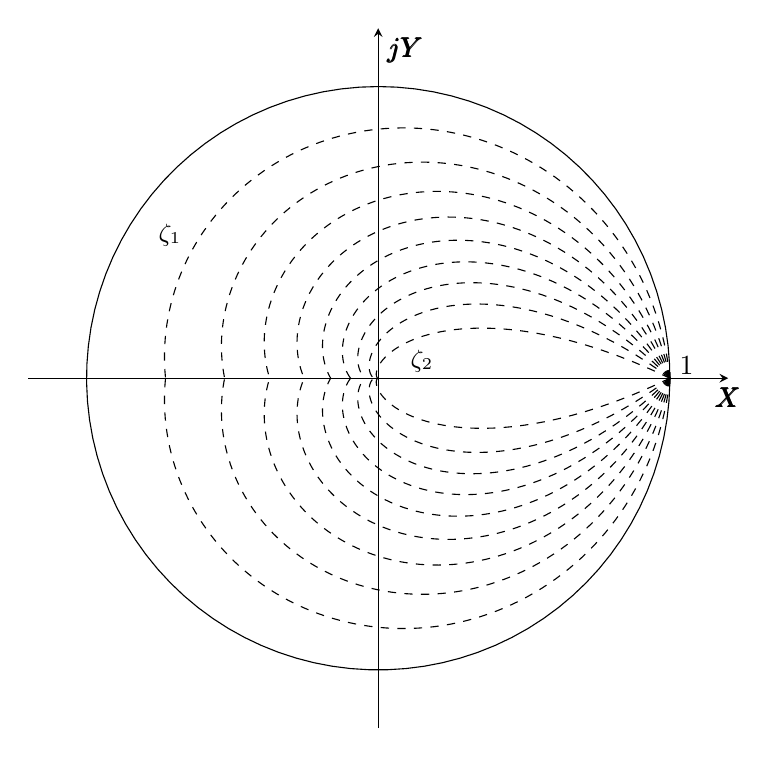
\begin{tikzpicture}

\begin{axis}[%
  axis lines=center,
  width=3.5in,
  height=3.5in,
  scale only axis,
  xmin=-1.2,
  xmax=1.2,
  ymin=-1.2,
  ymax=1.2,
  xtick={1},
  ytick=\empty,
  %xticklabels={},
  xticklabel style={anchor=south west},
  x label style={anchor=north},
  xlabel={$\pmb{X}$},
  ylabel={$\pmb{jY}$}
]
\addplot [color=black, forget plot]
  table[row sep=crcr]{%
0	1\\
0.0634239196565645	0.997986676471884\\
0.126592453573749	0.991954812830795\\
0.18925124436041	0.981928697262707\\
0.251147987181079	0.967948701396356\\
0.312033445698487	0.950071117740945\\
0.371662455660328	0.928367933016073\\
0.429794912089172	0.902926538286621\\
0.486196736100469	0.873849377069785\\
0.540640817455598	0.841253532831181\\
0.59290792905464	0.805270257531059\\
0.642787609686539	0.766044443118978\\
0.690079011482112	0.72373403810507\\
0.734591708657533	0.678509411557132\\
0.776146464291757	0.630552667084523\\
0.814575952050336	0.580056909571198\\
0.849725429949514	0.527225467610502\\
0.881453363447582	0.472271074772683\\
0.909631995354518	0.415415013001886\\
0.934147860265107	0.356886221591872\\
0.954902241444074	0.296920375328275\\
0.971811568323542	0.235758935509427\\
0.984807753012208	0.173648177666931\\
0.993838464461254	0.110838199901011\\
0.998867339183008	0.0475819158237424\\
0.999874127673875	-0.015865963834808\\
0.996854775951942	-0.0792499568567885\\
0.989821441880933	-0.142314838273285\\
0.978802446214779	-0.204806668065191\\
0.963842158559942	-0.266473813690035\\
0.945000818714669	-0.327067963317421\\
0.922354294104581	-0.386345125693128\\
0.895993774291336	-0.444066612605774\\
0.866025403784439	-0.5\\
0.832569854634771	-0.55392006386611\\
0.795761840530832	-0.605609687137666\\
0.755749574354258	-0.654860733945285\\
0.712694171378863	-0.701474887706321\\
0.666769000516292	-0.745264449675755\\
0.618158986220605	-0.786053094742787\\
0.567059863862771	-0.823676581429833\\
0.513677391573407	-0.857983413234977\\
0.458226521727411	-0.888835448654923\\
0.400930535406614	-0.916108457432069\\
0.342020143325669	-0.939692620785908\\
0.28173255684143	-0.959492973614497\\
0.220310532786541	-0.975429786885407\\
0.15800139597335	-0.987438888676394\\
0.0950560433041829	-0.995471922573085\\
0.0317279334980681	-0.999496542383185\\
-0.0317279334980679	-0.999496542383185\\
-0.0950560433041826	-0.995471922573085\\
-0.15800139597335	-0.987438888676394\\
-0.220310532786541	-0.975429786885407\\
-0.281732556841429	-0.959492973614497\\
-0.342020143325669	-0.939692620785908\\
-0.400930535406613	-0.91610845743207\\
-0.45822652172741	-0.888835448654924\\
-0.513677391573406	-0.857983413234977\\
-0.567059863862771	-0.823676581429833\\
-0.618158986220605	-0.786053094742788\\
-0.666769000516292	-0.745264449675755\\
-0.712694171378863	-0.701474887706322\\
-0.755749574354258	-0.654860733945285\\
-0.795761840530832	-0.605609687137667\\
-0.832569854634771	-0.55392006386611\\
-0.866025403784438	-0.5\\
-0.895993774291336	-0.444066612605774\\
-0.922354294104581	-0.386345125693129\\
-0.945000818714668	-0.327067963317422\\
-0.963842158559942	-0.266473813690035\\
-0.978802446214779	-0.204806668065191\\
-0.989821441880933	-0.142314838273285\\
-0.996854775951942	-0.0792499568567888\\
-0.999874127673875	-0.0158659638348076\\
-0.998867339183008	0.0475819158237424\\
-0.993838464461254	0.110838199901011\\
-0.984807753012208	0.17364817766693\\
-0.971811568323542	0.235758935509427\\
-0.954902241444074	0.296920375328275\\
-0.934147860265107	0.356886221591872\\
-0.909631995354519	0.415415013001886\\
-0.881453363447582	0.472271074772682\\
-0.849725429949514	0.527225467610502\\
-0.814575952050336	0.580056909571198\\
-0.776146464291757	0.630552667084522\\
-0.734591708657534	0.678509411557132\\
-0.690079011482113	0.723734038105069\\
-0.64278760968654	0.766044443118977\\
-0.59290792905464	0.805270257531059\\
-0.540640817455597	0.841253532831181\\
-0.486196736100469	0.873849377069785\\
-0.429794912089172	0.902926538286621\\
-0.371662455660328	0.928367933016072\\
-0.312033445698487	0.950071117740945\\
-0.251147987181079	0.967948701396356\\
-0.189251244360411	0.981928697262707\\
-0.12659245357375	0.991954812830795\\
-0.0634239196565654	0.997986676471884\\
-2.44929359829471e-16	1\\
};
\addplot [color=black, dashed, forget plot]
  table[row sep=crcr]{%
1	0\\
0.996355675894196	0.031311738544454\\
0.991744207915904	0.0623952568417635\\
0.986176266623562	0.0932211036444067\\
0.979663405858395	0.123760269148488\\
0.972218045703082	0.153984211042097\\
0.963853454686905	0.183864879925138\\
0.954583731259804	0.213374744079341\\
0.944423784558363	0.242486813567919\\
0.933389314487286	0.271174663645149\\
0.921496791140463	0.299412457456957\\
0.908763433586244	0.327174968014412\\
0.895207188041996	0.354437599422875\\
0.880846705463472	0.381176407350381\\
0.865701318574964	0.407368118719727\\
0.849791018366557	0.432990150609548\\
0.833136430085219	0.458020628350625\\
0.815758788746754	0.48243840280446\\
0.797679914195986	0.506223066812133\\
0.778922185742773	0.529354970802303\\
0.759508516401756	0.551815237548133\\
0.739462326763917	0.573585776063844\\
0.718807518528229	0.594649294632494\\
0.697568447721846	0.614989312957509\\
0.675769897637407	0.634590173431413\\
0.653437051516106	0.653437051516106\\
0.630595465005309	0.671515965229972\\
0.607271038419472	0.688813783738016\\
0.583489988833183	0.70531823504214\\
0.559278822035108	0.721017912769564\\
0.534664304371591	0.735902282058355\\
0.509673434508578	0.749961684539869\\
0.48433341514044	0.763187342418857\\
0.458671624674142	0.775571361652856\\
0.432715588917053	0.78710673423337\\
0.406492952796512	0.797787339572243\\
0.380031452139034	0.807607944997462\\
0.353358885536856	0.816564205363516\\
0.326503086329192	0.824652661782262\\
0.299491894725349	0.831870739481111\\
0.272353130096494	0.83821674479613\\
0.245114563462553	0.843689861308526\\
0.217803890200343	0.848290145133715\\
0.190448702998685	0.852018519373006\\
0.163076465085787	0.854876767738689\\
0.135714483753824	0.856867527364047\\
0.108389884205117	0.857994280810589\\
0.0811295837439053	0.858261347285484\\
0.0539602663371597	0.857673873082901\\
0.0269083575674107	0.856237821263645\\
5.22899666167123e-17	0.853959960588124\\
-0.0267389710133675	0.850847853718362\\
-0.0532830510734783	0.846909844705366\\
-0.0796070899941588	0.8421550457788\\
-0.105686314564419	0.836593323456462\\
-0.131496350792703	0.830235283991667\\
-0.157013245614411	0.823092258177157\\
-0.182213488044495	0.815176285524687\\
-0.2070740297576	0.806500097839947\\
-0.23157230507891	0.797077102212939\\
-0.255686250369537	0.786921363444393\\
-0.279394322791008	0.776047585929238\\
-0.302675518434107	0.764471095018548\\
-0.325509389798054	0.752207817881766\\
-0.347876062606756	0.739274263891364\\
-0.369756251949576	0.725687504552447\\
-0.391131277734848	0.711465153000104\\
-0.411983079445094	0.696625343087594\\
-0.432294230183688	0.681186708088743\\
-0.452047950003462	0.665168359038114\\
-0.47122811850853	0.648589862732789\\
-0.489819286721389	0.631471219419718\\
-0.507806688208121	0.613832840192814\\
-0.525176249455312	0.595695524124067\\
-0.541914599493101	0.577080435153081\\
-0.558009078759514	0.558009078759514\\
-0.573447747202083	0.538503278442984\\
-0.588219391613473	0.518585152035002\\
-0.602313532198671	0.49827708786755\\
-0.615720428372028	0.477601720822873\\
-0.628431083783263	0.456581908289041\\
-0.64043725057227	0.43524070604576\\
-0.651731432853363	0.413601344104843\\
-0.662306889430351	0.391687202529621\\
-0.672157635744576	0.369521787257474\\
-0.681278445058817	0.347128705949459\\
-0.689664848880689	0.324531643890898\\
-0.697313136629901	0.301754339966517\\
-0.704220354554473	0.278820562733578\\
-0.710384303901703	0.255754086616121\\
-0.715803538350409	0.232578668243255\\
-0.720477360711629	0.209318022954057\\
-0.724405818905681	0.185995801491425\\
-0.727589701224124	0.162635566906816\\
-0.730030530885834	0.139260771697509\\
-0.731730559897045	0.115894735197653\\
-0.732692762225847	0.0925606212439533\\
-0.732920826302222	0.0692814161364764\\
-0.732419146855338	0.0460799069146058\\
-0.731192816100364	0.0229786599677571\\
-0.729247614287671	8.9307075662324e-17\\
};
\addplot [color=black, dashed, forget plot]
  table[row sep=crcr]{%
1	-0\\
0.996355675894196	-0.031311738544454\\
0.991744207915904	-0.0623952568417635\\
0.986176266623562	-0.0932211036444067\\
0.979663405858395	-0.123760269148488\\
0.972218045703082	-0.153984211042097\\
0.963853454686905	-0.183864879925138\\
0.954583731259804	-0.213374744079341\\
0.944423784558363	-0.242486813567919\\
0.933389314487286	-0.271174663645149\\
0.921496791140463	-0.299412457456957\\
0.908763433586244	-0.327174968014412\\
0.895207188041996	-0.354437599422875\\
0.880846705463472	-0.381176407350381\\
0.865701318574964	-0.407368118719727\\
0.849791018366557	-0.432990150609548\\
0.833136430085219	-0.458020628350625\\
0.815758788746754	-0.48243840280446\\
0.797679914195986	-0.506223066812133\\
0.778922185742773	-0.529354970802303\\
0.759508516401756	-0.551815237548133\\
0.739462326763917	-0.573585776063844\\
0.718807518528229	-0.594649294632494\\
0.697568447721846	-0.614989312957509\\
0.675769897637407	-0.634590173431413\\
0.653437051516106	-0.653437051516106\\
0.630595465005309	-0.671515965229972\\
0.607271038419472	-0.688813783738016\\
0.583489988833183	-0.70531823504214\\
0.559278822035108	-0.721017912769564\\
0.534664304371591	-0.735902282058355\\
0.509673434508578	-0.749961684539869\\
0.48433341514044	-0.763187342418857\\
0.458671624674142	-0.775571361652856\\
0.432715588917053	-0.78710673423337\\
0.406492952796512	-0.797787339572243\\
0.380031452139034	-0.807607944997462\\
0.353358885536856	-0.816564205363516\\
0.326503086329192	-0.824652661782262\\
0.299491894725349	-0.831870739481111\\
0.272353130096494	-0.83821674479613\\
0.245114563462553	-0.843689861308526\\
0.217803890200343	-0.848290145133715\\
0.190448702998685	-0.852018519373006\\
0.163076465085787	-0.854876767738689\\
0.135714483753824	-0.856867527364047\\
0.108389884205117	-0.857994280810589\\
0.0811295837439053	-0.858261347285484\\
0.0539602663371597	-0.857673873082901\\
0.0269083575674107	-0.856237821263645\\
5.22899666167123e-17	-0.853959960588124\\
-0.0267389710133675	-0.850847853718362\\
-0.0532830510734783	-0.846909844705366\\
-0.0796070899941588	-0.8421550457788\\
-0.105686314564419	-0.836593323456462\\
-0.131496350792703	-0.830235283991667\\
-0.157013245614411	-0.823092258177157\\
-0.182213488044495	-0.815176285524687\\
-0.2070740297576	-0.806500097839947\\
-0.23157230507891	-0.797077102212939\\
-0.255686250369537	-0.786921363444393\\
-0.279394322791008	-0.776047585929238\\
-0.302675518434107	-0.764471095018548\\
-0.325509389798054	-0.752207817881766\\
-0.347876062606756	-0.739274263891364\\
-0.369756251949576	-0.725687504552447\\
-0.391131277734848	-0.711465153000104\\
-0.411983079445094	-0.696625343087594\\
-0.432294230183688	-0.681186708088743\\
-0.452047950003462	-0.665168359038114\\
-0.47122811850853	-0.648589862732789\\
-0.489819286721389	-0.631471219419718\\
-0.507806688208121	-0.613832840192814\\
-0.525176249455312	-0.595695524124067\\
-0.541914599493101	-0.577080435153081\\
-0.558009078759514	-0.558009078759514\\
-0.573447747202083	-0.538503278442984\\
-0.588219391613473	-0.518585152035002\\
-0.602313532198671	-0.49827708786755\\
-0.615720428372028	-0.477601720822873\\
-0.628431083783263	-0.456581908289041\\
-0.64043725057227	-0.43524070604576\\
-0.651731432853363	-0.413601344104843\\
-0.662306889430351	-0.391687202529621\\
-0.672157635744576	-0.369521787257474\\
-0.681278445058817	-0.347128705949459\\
-0.689664848880689	-0.324531643890898\\
-0.697313136629901	-0.301754339966517\\
-0.704220354554473	-0.278820562733578\\
-0.710384303901703	-0.255754086616121\\
-0.715803538350409	-0.232578668243255\\
-0.720477360711629	-0.209318022954057\\
-0.724405818905681	-0.185995801491425\\
-0.727589701224124	-0.162635566906816\\
-0.730030530885834	-0.139260771697509\\
-0.731730559897045	-0.115894735197653\\
-0.732692762225847	-0.0925606212439533\\
-0.732920826302222	-0.0692814161364764\\
-0.732419146855338	-0.0460799069146058\\
-0.731192816100364	-0.0229786599677571\\
-0.729247614287671	-8.9307075662324e-17\\
};
\addplot [color=black, dashed, forget plot]
  table[row sep=crcr]{%
1	0\\
0.993117483189145	0.0312099742390054\\
0.985308272923941	0.0619903421332781\\
0.97659215519062	0.0923151383768702\\
0.966989590174559	0.122159193890609\\
0.956521682769877	0.151498151383791\\
0.94521015280632	0.180308479888376\\
0.933077305027449	0.208567488263936\\
0.920145998853958	0.236253337672669\\
0.906439617965761	0.263345053024872\\
0.891982039736211	0.289822533396298\\
0.876797604551564	0.315666561419856\\
0.86091108504849	0.340858811655134\\
0.844347655302098	0.365381857940227\\
0.82713285999656	0.389219179731315\\
0.809292583610081	0.412355167436434\\
0.790853019645473	0.434775126750799\\
0.771840639937194	0.456465282001969\\
0.752282164065243	0.477412778514076\\
0.732204528905761	0.497605684001175\\
0.711634858347723	0.517032989000692\\
0.690600433204527	0.535684606358738\\
0.669128661348724	0.553551369779917\\
0.647247048097569	0.570625031455008\\
0.624983166876419	0.586898258780722\\
0.602364630186426	0.602364630186426\\
0.579419060902297	0.61701863008351\\
0.556174063925214	0.630855642953699\\
0.532657198215371	0.643871946593355\\
0.508895949227834	0.656064704531411\\
0.484917701774751	0.667431957639199\\
0.460749713336196	0.677972614951073\\
0.436419087841189	0.687686443715224\\
0.411952749939678	0.696574058694691\\
0.38737741978552	0.704636910739023\\
0.362719588349683	0.711877274647591\\
0.338005493282155	0.718298236345939\\
0.313261095340199	0.723903679397059\\
0.28851205539983	0.728698270869819\\
0.263783712066551	0.732687446587187\\
0.239101059900595	0.735877395777214\\
0.214488728271062	0.738275045150065\\
0.189970960852564	0.739888042424682\\
0.165571595777099	0.74072473932891\\
0.141314046453114	0.740794174097177\\
0.117221283062812	0.740106053489981\\
0.093315814747988	0.738670734359673\\
0.0696196724937937	0.736499204787132\\
0.0461543927190345	0.733603064814063\\
0.0229410015807486	0.729994506795762\\
4.44354699422903e-17	0.725686295399261\\
-0.0226486505850102	0.720691747271768\\
-0.0449855417332313	0.715024710404419\\
-0.0669918307779809	0.708699543216261\\
-0.0886492528634361	0.701731093383425\\
-0.109940132237539	0.694134676438339\\
-0.130847392799268	0.685926054163788\\
-0.151354567898984	0.677121412806495\\
-0.17144580939139	0.667737341134781\\
-0.191105895941341	0.657790808364695\\
-0.210320240583588	0.647299141978847\\
-0.229074897538198	0.63628000546197\\
-0.247356568284209	0.624751375976997\\
-0.265152606894742	0.612731522005231\\
-0.282451024637557	0.600238980973899\\
-0.299240493845688	0.587292536894097\\
-0.315510351063531	0.573911198031842\\
-0.331250599474388	0.560114174634617\\
-0.346451910616147	0.545920856735445\\
-0.361105625392428	0.531350792056182\\
-0.375203754387119	0.516423664031337\\
-0.388738977490884	0.501159269973318\\
-0.401704642848774	0.485577499399622\\
-0.414094765138671	0.469698312542032\\
-0.425904023190858	0.453541719057446\\
-0.437127756959533	0.437127756959533\\
-0.447761963857629	0.420476471789907\\
-0.457803294466788	0.40360789604704\\
-0.467249047634843	0.386542028890662\\
-0.47609716497361	0.369298816138837\\
-0.484346224770267	0.351898130574443\\
-0.491995435325994	0.334359752577216\\
-0.499044627735993	0.316703351096997\\
-0.505494248125377	0.298948464983263\\
-0.511345349355781	0.281114484685478\\
-0.516599582217932	0.263220634338226\\
-0.521259186125707	0.245285954244527\\
-0.525326979327546	0.227329283770144\\
-0.528806348651366	0.209369244661129\\
-0.531701238799399	0.191424224796241\\
-0.534016141209622	0.173512362385299\\
-0.535756082500673	0.155651530623926\\
-0.536926612517378	0.137859322814535\\
-0.53753379199418	0.120153037962827\\
-0.537584179853935	0.102549666858439\\
-0.537084820159711	0.0850658786478001\\
-0.536043228737323	0.0677180079066311\\
-0.534467379486475	0.0505220422189308\\
-0.532365690398461	0.0334936102686788\\
-0.529747009298427	0.016647970449882\\
-0.526620599330303	6.44924231334916e-17\\
};
\addplot [color=black, dashed, forget plot]
  table[row sep=crcr]{%
1	-0\\
0.993117483189145	-0.0312099742390054\\
0.985308272923941	-0.0619903421332781\\
0.97659215519062	-0.0923151383768702\\
0.966989590174559	-0.122159193890609\\
0.956521682769877	-0.151498151383791\\
0.94521015280632	-0.180308479888376\\
0.933077305027449	-0.208567488263936\\
0.920145998853958	-0.236253337672669\\
0.906439617965761	-0.263345053024872\\
0.891982039736211	-0.289822533396298\\
0.876797604551564	-0.315666561419856\\
0.86091108504849	-0.340858811655134\\
0.844347655302098	-0.365381857940227\\
0.82713285999656	-0.389219179731315\\
0.809292583610081	-0.412355167436434\\
0.790853019645473	-0.434775126750799\\
0.771840639937194	-0.456465282001969\\
0.752282164065243	-0.477412778514076\\
0.732204528905761	-0.497605684001175\\
0.711634858347723	-0.517032989000692\\
0.690600433204527	-0.535684606358738\\
0.669128661348724	-0.553551369779917\\
0.647247048097569	-0.570625031455008\\
0.624983166876419	-0.586898258780722\\
0.602364630186426	-0.602364630186426\\
0.579419060902297	-0.61701863008351\\
0.556174063925214	-0.630855642953699\\
0.532657198215371	-0.643871946593355\\
0.508895949227834	-0.656064704531411\\
0.484917701774751	-0.667431957639199\\
0.460749713336196	-0.677972614951073\\
0.436419087841189	-0.687686443715224\\
0.411952749939678	-0.696574058694691\\
0.38737741978552	-0.704636910739023\\
0.362719588349683	-0.711877274647591\\
0.338005493282155	-0.718298236345939\\
0.313261095340199	-0.723903679397059\\
0.28851205539983	-0.728698270869819\\
0.263783712066551	-0.732687446587187\\
0.239101059900595	-0.735877395777214\\
0.214488728271062	-0.738275045150065\\
0.189970960852564	-0.739888042424682\\
0.165571595777099	-0.74072473932891\\
0.141314046453114	-0.740794174097177\\
0.117221283062812	-0.740106053489981\\
0.093315814747988	-0.738670734359673\\
0.0696196724937937	-0.736499204787132\\
0.0461543927190345	-0.733603064814063\\
0.0229410015807486	-0.729994506795762\\
4.44354699422903e-17	-0.725686295399261\\
-0.0226486505850102	-0.720691747271768\\
-0.0449855417332313	-0.715024710404419\\
-0.0669918307779809	-0.708699543216261\\
-0.0886492528634361	-0.701731093383425\\
-0.109940132237539	-0.694134676438339\\
-0.130847392799268	-0.685926054163788\\
-0.151354567898984	-0.677121412806495\\
-0.17144580939139	-0.667737341134781\\
-0.191105895941341	-0.657790808364695\\
-0.210320240583588	-0.647299141978847\\
-0.229074897538198	-0.63628000546197\\
-0.247356568284209	-0.624751375976997\\
-0.265152606894742	-0.612731522005231\\
-0.282451024637557	-0.600238980973899\\
-0.299240493845688	-0.587292536894097\\
-0.315510351063531	-0.573911198031842\\
-0.331250599474388	-0.560114174634617\\
-0.346451910616147	-0.545920856735445\\
-0.361105625392428	-0.531350792056182\\
-0.375203754387119	-0.516423664031337\\
-0.388738977490884	-0.501159269973318\\
-0.401704642848774	-0.485577499399622\\
-0.414094765138671	-0.469698312542032\\
-0.425904023190858	-0.453541719057446\\
-0.437127756959533	-0.437127756959533\\
-0.447761963857629	-0.420476471789907\\
-0.457803294466788	-0.40360789604704\\
-0.467249047634843	-0.386542028890662\\
-0.47609716497361	-0.369298816138837\\
-0.484346224770267	-0.351898130574443\\
-0.491995435325994	-0.334359752577216\\
-0.499044627735993	-0.316703351096997\\
-0.505494248125377	-0.298948464983263\\
-0.511345349355781	-0.281114484685478\\
-0.516599582217932	-0.263220634338226\\
-0.521259186125707	-0.245285954244527\\
-0.525326979327546	-0.227329283770144\\
-0.528806348651366	-0.209369244661129\\
-0.531701238799399	-0.191424224796241\\
-0.534016141209622	-0.173512362385299\\
-0.535756082500673	-0.155651530623926\\
-0.536926612517378	-0.137859322814535\\
-0.53753379199418	-0.120153037962827\\
-0.537584179853935	-0.102549666858439\\
-0.537084820159711	-0.0850658786478001\\
-0.536043228737323	-0.0677180079066311\\
-0.534467379486475	-0.0505220422189308\\
-0.532365690398461	-0.0334936102686788\\
-0.529747009298427	-0.016647970449882\\
-0.526620599330303	-6.44924231334916e-17\\
};
\addplot [color=black, dashed, forget plot]
  table[row sep=crcr]{%
1	0\\
0.989680205048008	0.031101953421677\\
0.978499576757223	0.0615619752795178\\
0.966486964076787	0.0913599165772274\\
0.953671544913749	0.120476733510694\\
0.940082788364644	0.148894486293864\\
0.925750417373368	0.176596336822066\\
0.910704371847075	0.203566545198034\\
0.894974772260769	0.22979046514661\\
0.878591883780097	0.255254538344805\\
0.86158608093073	0.279946287694513\\
0.843987812841589	0.303854309565807\\
0.825827569087992	0.326968265039271\\
0.807135846159684	0.349278870176369\\
0.787943114577512	0.37077788534731\\
0.768279786681378	0.391458103646313\\
0.748176185110921	0.411313338424568\\
0.727662511999217	0.430338409971535\\
0.70676881889864	0.448529131375562\\
0.685524977456837	0.465882293595051\\
0.663960650859636	0.482395649771645\\
0.642105266056556	0.498067898817131\\
0.619987986783415	0.512898668305873\\
0.597637687395423	0.526888496704744\\
0.575082927522991	0.540038814972599\\
0.552351927561387	0.552351927561387\\
0.529472545004228	0.563830992851004\\
0.506472251629725	0.574480003049982\\
0.483378111547487	0.584303763594046\\
0.460216760112624	0.593307872074486\\
0.437014383712816	0.601498696728173\\
0.41379670043299	0.608883354520886\\
0.390588941601167	0.61546968885546\\
0.367415834218091	0.621266246936007\\
0.344301584272182	0.626282256819272\\
0.321269860940431	0.630527604183869\\
0.298343781674863	0.634012808847879\\
0.275545898173243	0.636749001064931\\
0.252898183231812	0.638747897628573\\
0.23042201847689	0.640021777814333\\
0.208138182971344	0.640583459188477\\
0.186066842691023	0.640446273312061\\
0.164227540865449	0.639624041368408\\
0.142639189176222	0.638131049741675\\
0.121320059805814	0.635982025573706\\
0.100287778328637	0.633192112325829\\
0.0795593174355637	0.629776845371748\\
0.0591509914823055	0.625752127647141\\
0.0390784518514043	0.621134205380978\\
0.019356683116887	0.615939643933052\\
3.73630739569175e-17	0.610185303761559\\
-0.0189779548961836	0.603888316544021\\
-0.0375642125860939	0.597066061474163\\
-0.055746478448306	0.589736141756782\\
-0.0735131322334228	0.581916361321951\\
-0.0908532273476422	0.573624701779294\\
-0.107756489426951	0.564879299632359\\
-0.124213314217353	0.555698423772488\\
-0.140214764776994	0.54610045327087\\
-0.155752568016441	0.536103855486799\\
-0.170819110593797	0.525727164509449\\
-0.185407434181671	0.514988959949799\\
-0.199511230123377	0.503907846098627\\
-0.213124833496062	0.49250243146579\\
-0.226243216598717	0.480791308715308\\
-0.23886198188335	0.468793035010043\\
-0.250977354347776	0.456526112779072\\
-0.262586173408747	0.444008970920142\\
-0.273685884274306	0.431259946448866\\
-0.284274528834428	0.418297266605636\\
-0.294350736089166	0.40513903143051\\
-0.303913712133613	0.391803196815617\\
-0.312963229719119	0.378307558043956\\
-0.321499617410256	0.364669733822732\\
-0.329523748357088	0.350907150818703\\
-0.337037028702328	0.337037028702328\\
-0.344041385642971	0.323076365706811\\
-0.350539255165994	0.309041924707485\\
-0.356533569477655	0.294950219826293\\
-0.362027744145895	0.280817503565482\\
-0.367025664975262	0.266659754473976\\
-0.371531674633684	0.252492665349235\\
-0.375550559050301	0.238331631976814\\
-0.379087533603451	0.224191742409173\\
-0.382148229117742	0.210087766784708\\
-0.384738677688982	0.196034147687371\\
-0.386865298355562	0.182044991046649\\
-0.388534882634674	0.168134057577092\\
-0.389754579941548	0.15431475475605\\
-0.390531882909652	0.140600129337673\\
-0.390874612629551	0.127002860400749\\
-0.390790903823879	0.113535252927376\\
-0.390289189975578	0.100209231908998\\
-0.389378188426307	0.0870363369757959\\
-0.388066885461584	0.0740277175449813\\
-0.386364521398959	0.0611941284830315\\
-0.384280575695157	0.0485459262764819\\
-0.381824752087813	0.0360930657054282\\
-0.379006963787087	0.0238450970134807\\
-0.375837318732076	0.0118111635674941\\
-0.372326104926586	4.55967972637346e-17\\
};
\addplot [color=black, dashed, forget plot]
  table[row sep=crcr]{%
1	-0\\
0.989680205048008	-0.031101953421677\\
0.978499576757223	-0.0615619752795178\\
0.966486964076787	-0.0913599165772274\\
0.953671544913749	-0.120476733510694\\
0.940082788364644	-0.148894486293864\\
0.925750417373368	-0.176596336822066\\
0.910704371847075	-0.203566545198034\\
0.894974772260769	-0.22979046514661\\
0.878591883780097	-0.255254538344805\\
0.86158608093073	-0.279946287694513\\
0.843987812841589	-0.303854309565807\\
0.825827569087992	-0.326968265039271\\
0.807135846159684	-0.349278870176369\\
0.787943114577512	-0.37077788534731\\
0.768279786681378	-0.391458103646313\\
0.748176185110921	-0.411313338424568\\
0.727662511999217	-0.430338409971535\\
0.70676881889864	-0.448529131375562\\
0.685524977456837	-0.465882293595051\\
0.663960650859636	-0.482395649771645\\
0.642105266056556	-0.498067898817131\\
0.619987986783415	-0.512898668305873\\
0.597637687395423	-0.526888496704744\\
0.575082927522991	-0.540038814972599\\
0.552351927561387	-0.552351927561387\\
0.529472545004228	-0.563830992851004\\
0.506472251629725	-0.574480003049982\\
0.483378111547487	-0.584303763594046\\
0.460216760112624	-0.593307872074486\\
0.437014383712816	-0.601498696728173\\
0.41379670043299	-0.608883354520886\\
0.390588941601167	-0.61546968885546\\
0.367415834218091	-0.621266246936007\\
0.344301584272182	-0.626282256819272\\
0.321269860940431	-0.630527604183869\\
0.298343781674863	-0.634012808847879\\
0.275545898173243	-0.636749001064931\\
0.252898183231812	-0.638747897628573\\
0.23042201847689	-0.640021777814333\\
0.208138182971344	-0.640583459188477\\
0.186066842691023	-0.640446273312061\\
0.164227540865449	-0.639624041368408\\
0.142639189176222	-0.638131049741675\\
0.121320059805814	-0.635982025573706\\
0.100287778328637	-0.633192112325829\\
0.0795593174355637	-0.629776845371748\\
0.0591509914823055	-0.625752127647141\\
0.0390784518514043	-0.621134205380978\\
0.019356683116887	-0.615939643933052\\
3.73630739569175e-17	-0.610185303761559\\
-0.0189779548961836	-0.603888316544021\\
-0.0375642125860939	-0.597066061474163\\
-0.055746478448306	-0.589736141756782\\
-0.0735131322334228	-0.581916361321951\\
-0.0908532273476422	-0.573624701779294\\
-0.107756489426951	-0.564879299632359\\
-0.124213314217353	-0.555698423772488\\
-0.140214764776994	-0.54610045327087\\
-0.155752568016441	-0.536103855486799\\
-0.170819110593797	-0.525727164509449\\
-0.185407434181671	-0.514988959949799\\
-0.199511230123377	-0.503907846098627\\
-0.213124833496062	-0.49250243146579\\
-0.226243216598717	-0.480791308715308\\
-0.23886198188335	-0.468793035010043\\
-0.250977354347776	-0.456526112779072\\
-0.262586173408747	-0.444008970920142\\
-0.273685884274306	-0.431259946448866\\
-0.284274528834428	-0.418297266605636\\
-0.294350736089166	-0.40513903143051\\
-0.303913712133613	-0.391803196815617\\
-0.312963229719119	-0.378307558043956\\
-0.321499617410256	-0.364669733822732\\
-0.329523748357088	-0.350907150818703\\
-0.337037028702328	-0.337037028702328\\
-0.344041385642971	-0.323076365706811\\
-0.350539255165994	-0.309041924707485\\
-0.356533569477655	-0.294950219826293\\
-0.362027744145895	-0.280817503565482\\
-0.367025664975262	-0.266659754473976\\
-0.371531674633684	-0.252492665349235\\
-0.375550559050301	-0.238331631976814\\
-0.379087533603451	-0.224191742409173\\
-0.382148229117742	-0.210087766784708\\
-0.384738677688982	-0.196034147687371\\
-0.386865298355562	-0.182044991046649\\
-0.388534882634674	-0.168134057577092\\
-0.389754579941548	-0.15431475475605\\
-0.390531882909652	-0.140600129337673\\
-0.390874612629551	-0.127002860400749\\
-0.390790903823879	-0.113535252927376\\
-0.390289189975578	-0.100209231908998\\
-0.389378188426307	-0.0870363369757959\\
-0.388066885461584	-0.0740277175449813\\
-0.386364521398959	-0.0611941284830315\\
-0.384280575695157	-0.0485459262764819\\
-0.381824752087813	-0.0360930657054282\\
-0.379006963787087	-0.0238450970134807\\
-0.375837318732076	-0.0118111635674941\\
-0.372326104926586	-4.55967972637346e-17\\
};
\addplot [color=black, dashed, forget plot]
  table[row sep=crcr]{%
1	0\\
0.985895813452101	0.0309830241245718\\
0.971030607198477	0.0610920675450016\\
0.955442193368263	0.0903158783562781\\
0.93916819939932	0.118644534886467\\
0.922246029428501	0.146069421212559\\
0.904712826985092	0.172583201825407\\
0.886605438995365	0.198179795496117\\
0.867960381104534	0.222854348395785\\
0.848813804320638	0.246603206519935\\
0.829201462983264	0.269423887468404\\
0.809158684058388	0.29131505163083\\
0.788720337759048	0.312276472827206\\
0.767920809490031	0.33230900845226\\
0.746793973113281	0.351414569171693\\
0.725373165529273	0.369596088217499\\
0.703691162568218	0.386857490328817\\
0.681780156183619	0.403203660383866\\
0.659671732939361	0.418640411767708\\
0.637396853780289	0.433174454519605\\
0.614985835074999	0.446813363302878\\
0.592468330918392	0.459565545239158\\
0.56987331668043	0.471440207648008\\
0.547229073786448	0.48244732573182\\
0.524563175713346	0.492597610244956\\
0.501902475185001	0.501902475185001\\
0.4792730925493	0.510374005542979\\
0.456700405318304	0.518024925148315\\
0.434209038852194	0.524868564643241\\
0.411822858166868	0.530918829620249\\
0.38956496084428	0.536190168955128\\
0.367457671023913	0.540697543366961\\
0.3455225344531	0.544456394235416\\
0.323780314573297	0.547482612704467\\
0.302250989618812	0.549792509100638\\
0.280953750703967	0.551402782692681\\
0.259907000874183	0.552330491818503\\
0.239128355096	0.552593024404032\\
0.218634641160653	0.552208068897579\\
0.198441901475454	0.55119358564214\\
0.178565395716864	0.549567778706978\\
0.159019604318909	0.54734906819869\\
0.13981823277026	0.54455606307089\\
0.120974216693163	0.541207534450524\\
0.102499727677157	0.537322389497761\\
0.0844061798404073	0.532919645815306\\
0.0667042370913888	0.528018406421945\\
0.0494038210635276	0.522637835304059\\
0.0325141196954289	0.516797133557798\\
0.0160435964292729	0.510515516133592\\
3.08495992433718e-17	0.50381218919366\\
-0.0156096252120404	0.496706328092168\\
-0.0307789282922142	0.489217055986714\\
-0.0455022403936249	0.481363423088857\\
-0.0597745628570143	0.473164386560439\\
-0.0735915548753502	0.464638791061534\\
-0.0869495207297097	0.455805349954945\\
-0.0998453966228506	0.446682627171261\\
-0.112276737136607	0.437289019737639\\
-0.124241701338985	0.42764274097258\\
-0.135739038566523	0.417761804348184\\
-0.146768073907193	0.407664008020518\\
-0.157328693408749	0.397366920027949\\
-0.167421329037108	0.38688786415654\\
-0.177046943408938	0.376243906470834\\
-0.186207014322271	0.365451842507638\\
-0.194903519108526	0.354528185129726\\
-0.203138918828893	0.343489153035665\\
-0.210916142337624	0.332350659921355\\
-0.218238570234292	0.321128304288199\\
-0.225110018726605	0.309837359892227\\
-0.231534723424919	0.298492766827909\\
-0.237517323089057	0.287109123239819\\
-0.243062843347575	0.275700677654769\\
-0.248176680409077	0.264281321926519\\
-0.252864584784672	0.252864584784672\\
-0.257132645040145	0.241463625978879\\
-0.260987271595855	0.230091231009047\\
-0.264435180591845	0.218759806431799\\
-0.267483377835114	0.20748137573304\\
-0.270139142845402	0.196267575756099\\
-0.272410013015343	0.185129653674561\\
-0.274303767900232	0.174078464498558\\
-0.275828413652103	0.163124469102985\\
-0.276992167612268	0.152277732765804\\
-0.277803443075876	0.141547924204336\\
-0.278270834241491	0.130944315097181\\
-0.278403101358141	0.120475780079195\\
-0.278209156081693	0.110150797196719\\
-0.27769804705187	0.0999774488101011\\
-0.27687894570066	0.0899634229303457\\
-0.275761132302292	0.0801160149766191\\
-0.274353982274426	0.0704421299411734\\
-0.272666952739622	0.060948284948171\\
-0.270709569355636	0.0516406121927823\\
-0.268491413422519	0.0425248622468694\\
-0.266022109273988	0.0336064077175056\\
-0.263311311959974	0.0248902472445477\\
-0.260368695226763	0.0163810098234588\\
-0.257203939800597	0.00808295943957172\\
-0.253826721980109	3.10848082611005e-17\\
};
\addplot [color=black, dashed, forget plot]
  table[row sep=crcr]{%
1	-0\\
0.985895813452101	-0.0309830241245718\\
0.971030607198477	-0.0610920675450016\\
0.955442193368263	-0.0903158783562781\\
0.93916819939932	-0.118644534886467\\
0.922246029428501	-0.146069421212559\\
0.904712826985092	-0.172583201825407\\
0.886605438995365	-0.198179795496117\\
0.867960381104534	-0.222854348395785\\
0.848813804320638	-0.246603206519935\\
0.829201462983264	-0.269423887468404\\
0.809158684058388	-0.29131505163083\\
0.788720337759048	-0.312276472827206\\
0.767920809490031	-0.33230900845226\\
0.746793973113281	-0.351414569171693\\
0.725373165529273	-0.369596088217499\\
0.703691162568218	-0.386857490328817\\
0.681780156183619	-0.403203660383866\\
0.659671732939361	-0.418640411767708\\
0.637396853780289	-0.433174454519605\\
0.614985835074999	-0.446813363302878\\
0.592468330918392	-0.459565545239158\\
0.56987331668043	-0.471440207648008\\
0.547229073786448	-0.48244732573182\\
0.524563175713346	-0.492597610244956\\
0.501902475185001	-0.501902475185001\\
0.4792730925493	-0.510374005542979\\
0.456700405318304	-0.518024925148315\\
0.434209038852194	-0.524868564643241\\
0.411822858166868	-0.530918829620249\\
0.38956496084428	-0.536190168955128\\
0.367457671023913	-0.540697543366961\\
0.3455225344531	-0.544456394235416\\
0.323780314573297	-0.547482612704467\\
0.302250989618812	-0.549792509100638\\
0.280953750703967	-0.551402782692681\\
0.259907000874183	-0.552330491818503\\
0.239128355096	-0.552593024404032\\
0.218634641160653	-0.552208068897579\\
0.198441901475454	-0.55119358564214\\
0.178565395716864	-0.549567778706978\\
0.159019604318909	-0.54734906819869\\
0.13981823277026	-0.54455606307089\\
0.120974216693163	-0.541207534450524\\
0.102499727677157	-0.537322389497761\\
0.0844061798404073	-0.532919645815306\\
0.0667042370913888	-0.528018406421945\\
0.0494038210635276	-0.522637835304059\\
0.0325141196954289	-0.516797133557798\\
0.0160435964292729	-0.510515516133592\\
3.08495992433718e-17	-0.50381218919366\\
-0.0156096252120404	-0.496706328092168\\
-0.0307789282922142	-0.489217055986714\\
-0.0455022403936249	-0.481363423088857\\
-0.0597745628570143	-0.473164386560439\\
-0.0735915548753502	-0.464638791061534\\
-0.0869495207297097	-0.455805349954945\\
-0.0998453966228506	-0.446682627171261\\
-0.112276737136607	-0.437289019737639\\
-0.124241701338985	-0.42764274097258\\
-0.135739038566523	-0.417761804348184\\
-0.146768073907193	-0.407664008020518\\
-0.157328693408749	-0.397366920027949\\
-0.167421329037108	-0.38688786415654\\
-0.177046943408938	-0.376243906470834\\
-0.186207014322271	-0.365451842507638\\
-0.194903519108526	-0.354528185129726\\
-0.203138918828893	-0.343489153035665\\
-0.210916142337624	-0.332350659921355\\
-0.218238570234292	-0.321128304288199\\
-0.225110018726605	-0.309837359892227\\
-0.231534723424919	-0.298492766827909\\
-0.237517323089057	-0.287109123239819\\
-0.243062843347575	-0.275700677654769\\
-0.248176680409077	-0.264281321926519\\
-0.252864584784672	-0.252864584784672\\
-0.257132645040145	-0.241463625978879\\
-0.260987271595855	-0.230091231009047\\
-0.264435180591845	-0.218759806431799\\
-0.267483377835114	-0.20748137573304\\
-0.270139142845402	-0.196267575756099\\
-0.272410013015343	-0.185129653674561\\
-0.274303767900232	-0.174078464498558\\
-0.275828413652103	-0.163124469102985\\
-0.276992167612268	-0.152277732765804\\
-0.277803443075876	-0.141547924204336\\
-0.278270834241491	-0.130944315097181\\
-0.278403101358141	-0.120475780079195\\
-0.278209156081693	-0.110150797196719\\
-0.27769804705187	-0.0999774488101011\\
-0.27687894570066	-0.0899634229303457\\
-0.275761132302292	-0.0801160149766191\\
-0.274353982274426	-0.0704421299411734\\
-0.272666952739622	-0.060948284948171\\
-0.270709569355636	-0.0516406121927823\\
-0.268491413422519	-0.0425248622468694\\
-0.266022109273988	-0.0336064077175056\\
-0.263311311959974	-0.0248902472445477\\
-0.260368695226763	-0.0163810098234588\\
-0.257203939800597	-0.00808295943957172\\
-0.253826721980109	-3.10848082611005e-17\\
};
\addplot [color=black, dashed, forget plot]
  table[row sep=crcr]{%
1	0\\
0.981540939422561	0.0308461666947342\\
0.962471129762764	0.0605535508702686\\
0.942836971950334	0.0891243341141066\\
0.922683943103812	0.116562089034509\\
0.902056570675584	0.142871725087523\\
0.880998408745192	0.168059434606468\\
0.859552016415043	0.192132639096407\\
0.83775893826151	0.215099935853556\\
0.815659686793484	0.23697104496705\\
0.793293726869509	0.257756756757911\\
0.770699462023874	0.277468879707576\\
0.747914222651314	0.29612018892583\\
0.724974255999383	0.313724375205511\\
0.701914717917016	0.330295994708921\\
0.678769666307395	0.345850419328459\\
0.655572056232849	0.360403787761589\\
0.632353736619263	0.373972957337927\\
0.609145448507269	0.386575456633898\\
0.58597682479738	0.398229438908136\\
0.562876391436159	0.408953636388562\\
0.539871569990569	0.418767315439871\\
0.516988681557711	0.427690232637992\\
0.494252951957326	0.435742591775968\\
0.47168851815465	0.442945001823645\\
0.449318435861499	0.449318435861499\\
0.427164688263771	0.454884191006973\\
0.405248195823966	0.459663849349744\\
0.383588827107768	0.463679239910464\\
0.362205410584191	0.46695240163566\\
0.341115747349381	0.469505547439701\\
0.320336624724713	0.471361029303006\\
0.299883830680465	0.472541304433944\\
0.279772169037023	0.473068902500281\\
0.260015475396269	0.472966393934389\\
0.24062663375655	0.472256359314945\\
0.221617593765415	0.470961359826317\\
0.202999388565092	0.469103908795423\\
0.184782153186531	0.466706444304463\\
0.166975143448709	0.463791302876569\\
0.149586755320764	0.460380694230177\\
0.132624544705454	0.456496677096648\\
0.116095247603365	0.452161136094518\\
0.10000480061825	0.447395759652626\\
0.0843583617648406	0.442222018973253\\
0.0691603315414791	0.436661148025441\\
0.0544143742308923	0.430734124557617\\
0.0401234393934662	0.424461652117753\\
0.0262897835183805	0.417864143068408\\
0.0129149917990066	0.410961702583145\\
2.47240337905553e-17	0.403774113610049\\
-0.0124548836154341	0.396320822787319\\
-0.0244499563285837	0.388620927295222\\
-0.0359860990080092	0.380693162628028\\
-0.0470647541804444	0.372555891268966\\
-0.0576879041571531	0.364227092250654\\
-0.0678580492420327	0.355724351582953\\
-0.0775781860467111	0.347064853529714\\
-0.0868517859368481	0.338265372715437\\
-0.0956827736328178	0.329342267042489\\
-0.104075505986926	0.320311471399148\\
-0.1120347509583	0.311188492138431\\
-0.119565666805567	0.301988402307383\\
-0.126673781516471	0.292725837606255\\
-0.133364972492544	0.28341499305679\\
-0.139645446506012	0.274069620358657\\
-0.14552171994514	0.264703025912935\\
-0.15100059936325	0.255328069491445\\
-0.156089162345752	0.245957163530618\\
-0.16079473870856	0.236602273028593\\
-0.165124892040398	0.227274916024158\\
-0.169087401600594	0.217986164636207\\
-0.172690244583081	0.208746646642393\\
-0.175941578756487	0.199566547575719\\
-0.178849725489344	0.190455613317931\\
-0.18142315316863	0.18142315316863\\
-0.183670461019064	0.172478043369217\\
-0.185600363329776	0.163628731060893\\
-0.187221674094229	0.154883238656157\\
-0.188543292068522	0.146249168603396\\
-0.189574186252466	0.137733708524426\\
-0.190323381797141	0.129343636705056\\
-0.190799946341952	0.121085327918991\\
-0.191012976783529	0.112964759565685\\
-0.190971586478199	0.104987518103024\\
-0.190684892879101	0.0971588057560207\\
-0.190162005608454	0.0894834474830224\\
-0.189412014964881	0.0819658981812518\\
-0.188443980865132	0.0746102501138477\\
-0.187266922219036	0.0674202405409131\\
-0.185889806735969	0.0603992595374446\\
-0.184321541160631	0.0535503579813809\\
-0.182570961935477	0.0468762556953878\\
-0.180646826286633	0.0403793497263835\\
-0.178557803729771	0.0340617227471944\\
-0.176312467991919	0.0279251515651378\\
-0.173919289344852	0.021971115722724\\
-0.171386627345303	0.0162008061760833\\
-0.168722723976869	0.0106151340371341\\
-0.165935697188186	0.00521473936592495\\
-0.16303353482158	1.99658496572927e-17\\
};
\addplot [color=black, dashed, forget plot]
  table[row sep=crcr]{%
1	-0\\
0.981540939422561	-0.0308461666947342\\
0.962471129762764	-0.0605535508702686\\
0.942836971950334	-0.0891243341141066\\
0.922683943103812	-0.116562089034509\\
0.902056570675584	-0.142871725087523\\
0.880998408745192	-0.168059434606468\\
0.859552016415043	-0.192132639096407\\
0.83775893826151	-0.215099935853556\\
0.815659686793484	-0.23697104496705\\
0.793293726869509	-0.257756756757911\\
0.770699462023874	-0.277468879707576\\
0.747914222651314	-0.29612018892583\\
0.724974255999383	-0.313724375205511\\
0.701914717917016	-0.330295994708921\\
0.678769666307395	-0.345850419328459\\
0.655572056232849	-0.360403787761589\\
0.632353736619263	-0.373972957337927\\
0.609145448507269	-0.386575456633898\\
0.58597682479738	-0.398229438908136\\
0.562876391436159	-0.408953636388562\\
0.539871569990569	-0.418767315439871\\
0.516988681557711	-0.427690232637992\\
0.494252951957326	-0.435742591775968\\
0.47168851815465	-0.442945001823645\\
0.449318435861499	-0.449318435861499\\
0.427164688263771	-0.454884191006973\\
0.405248195823966	-0.459663849349744\\
0.383588827107768	-0.463679239910464\\
0.362205410584191	-0.46695240163566\\
0.341115747349381	-0.469505547439701\\
0.320336624724713	-0.471361029303006\\
0.299883830680465	-0.472541304433944\\
0.279772169037023	-0.473068902500281\\
0.260015475396269	-0.472966393934389\\
0.24062663375655	-0.472256359314945\\
0.221617593765415	-0.470961359826317\\
0.202999388565092	-0.469103908795423\\
0.184782153186531	-0.466706444304463\\
0.166975143448709	-0.463791302876569\\
0.149586755320764	-0.460380694230177\\
0.132624544705454	-0.456496677096648\\
0.116095247603365	-0.452161136094518\\
0.10000480061825	-0.447395759652626\\
0.0843583617648406	-0.442222018973253\\
0.0691603315414791	-0.436661148025441\\
0.0544143742308923	-0.430734124557617\\
0.0401234393934662	-0.424461652117753\\
0.0262897835183805	-0.417864143068408\\
0.0129149917990066	-0.410961702583145\\
2.47240337905553e-17	-0.403774113610049\\
-0.0124548836154341	-0.396320822787319\\
-0.0244499563285837	-0.388620927295222\\
-0.0359860990080092	-0.380693162628028\\
-0.0470647541804444	-0.372555891268966\\
-0.0576879041571531	-0.364227092250654\\
-0.0678580492420327	-0.355724351582953\\
-0.0775781860467111	-0.347064853529714\\
-0.0868517859368481	-0.338265372715437\\
-0.0956827736328178	-0.329342267042489\\
-0.104075505986926	-0.320311471399148\\
-0.1120347509583	-0.311188492138431\\
-0.119565666805567	-0.301988402307383\\
-0.126673781516471	-0.292725837606255\\
-0.133364972492544	-0.28341499305679\\
-0.139645446506012	-0.274069620358657\\
-0.14552171994514	-0.264703025912935\\
-0.15100059936325	-0.255328069491445\\
-0.156089162345752	-0.245957163530618\\
-0.16079473870856	-0.236602273028593\\
-0.165124892040398	-0.227274916024158\\
-0.169087401600594	-0.217986164636207\\
-0.172690244583081	-0.208746646642393\\
-0.175941578756487	-0.199566547575719\\
-0.178849725489344	-0.190455613317931\\
-0.18142315316863	-0.18142315316863\\
-0.183670461019064	-0.172478043369217\\
-0.185600363329776	-0.163628731060893\\
-0.187221674094229	-0.154883238656157\\
-0.188543292068522	-0.146249168603396\\
-0.189574186252466	-0.137733708524426\\
-0.190323381797141	-0.129343636705056\\
-0.190799946341952	-0.121085327918991\\
-0.191012976783529	-0.112964759565685\\
-0.190971586478199	-0.104987518103024\\
-0.190684892879101	-0.0971588057560207\\
-0.190162005608454	-0.0894834474830224\\
-0.189412014964881	-0.0819658981812518\\
-0.188443980865132	-0.0746102501138477\\
-0.187266922219036	-0.0674202405409131\\
-0.185889806735969	-0.0603992595374446\\
-0.184321541160631	-0.0535503579813809\\
-0.182570961935477	-0.0468762556953878\\
-0.180646826286633	-0.0403793497263835\\
-0.178557803729771	-0.0340617227471944\\
-0.176312467991919	-0.0279251515651378\\
-0.173919289344852	-0.021971115722724\\
-0.171386627345303	-0.0162008061760833\\
-0.168722723976869	-0.0106151340371341\\
-0.165935697188186	-0.00521473936592495\\
-0.16303353482158	-1.99658496572927e-17\\
};
\addplot [color=black, dashed, forget plot]
  table[row sep=crcr]{%
1	0\\
0.97623152123716	0.0306793115063044\\
0.952086762902519	0.0599002218846165\\
0.927619411331595	0.0876858511129781\\
0.902881167512372	0.114060416702534\\
0.877921760602431	0.139049146701748\\
0.852788963793768	0.162678195183061\\
0.827528612393348	0.184974560225043\\
0.802184623990148	0.205966004398664\\
0.776799020582307	0.225680977762209\\
0.751411952540787	0.244148543365328\\
0.726061724288963	0.26139830525893\\
0.700784821580431	0.277460339004006\\
0.675615940260427	0.292365124669015\\
0.650588016399211	0.306143482302199\\
0.625732257688895	0.318826509862098\\
0.601078175998265	0.330445523586591\\
0.576653620983267	0.34103200077804\\
0.552484814653924	0.350617524979482\\
0.528596386801616	0.359233733514399\\
0.505011411193747	0.36691226736026\\
0.481751442445967	0.373684723323934\\
0.458836553485221	0.379582608485022\\
0.436285373520005	0.384637296871355\\
0.414115126437298	0.388879988329137\\
0.392341669548685	0.392341669548685\\
0.370979532611252	0.395053077205228\\
0.35004195705183	0.397044663172925\\
0.329540935326143	0.39834656176907\\
0.309487250347379	0.398988558984361\\
0.289890514921595	0.399000063654162\\
0.270759211130251	0.398410080524829\\
0.252100729602985	0.39724718516844\\
0.233921408626535	0.395539500698623\\
0.216226573038441	0.39331467623965\\
0.199020572856858	0.390599867100522\\
0.182306821600443	0.387421716605414\\
0.166087834254868	0.38380633953162\\
0.15036526484503	0.379779307105932\\
0.135139943574541	0.375365633510327\\
0.120411913496453	0.370589763847805\\
0.106180466681585	0.36547556351929\\
0.0924441798530851	0.360046308962654\\
0.0792009494581386	0.354324679705094\\
0.0664480261499019	0.348332751680395\\
0.0541820486548744	0.34209199176291\\
0.0423990770029874	0.335623253470488\\
0.0310946250996974	0.328946773789014\\
0.0202636926213098	0.322082171071711\\
0.0099007962166476	0.315048443966901\\
1.88512313530119e-17	0.307863971328499\\
-0.00944505467795492	0.300546513064134\\
-0.0184411201928563	0.293113211876465\\
-0.026995314352961	0.285580595853949\\
-0.0351150928574258	0.277964581868071\\
-0.042808222513439	0.270280479734772\\
-0.0500827552176099	0.262542997098665\\
-0.0569470027056244	0.254766244999378\\
-0.0634095120728358	0.246963744080266\\
-0.0694790420671723	0.239148431400557\\
-0.075164540154518	0.231332667812908\\
-0.0804751203555534	0.223528245869218\\
-0.085420041851925	0.215746398218485\\
-0.0900086883585548	0.207997806461413\\
-0.0942505482578912	0.200292610427392\\
-0.0981551954909504	0.192640417840451\\
-0.101732271199093	0.185050314341716\\
-0.104991466109631	0.177530873836868\\
-0.107942503657553	0.170090169138047\\
-0.110595123834906	0.162735782870641\\
-0.112959067758674	0.155474818616317\\
-0.115044062947298	0.148313912264648\\
-0.11685980929543	0.141259243546641\\
-0.118415965735874	0.134316547724406\\
-0.119722137577188	0.12749112741219\\
-0.120787864504912	0.120787864504912\\
-0.121622609233946	0.114211232191291\\
-0.122235746799203	0.107765307029576\\
-0.122636554471279	0.101453781064815\\
-0.122834202283561	0.0952799739674815\\
-0.122837744156894	0.0892468451742257\\
-0.122656109607681	0.0833570060123306\\
-0.122298096025023	0.0776127317903872\\
-0.12177236150237	0.0720159738385218\\
-0.121087418208922	0.0665683714823661\\
-0.120251626285951	0.061271263935785\\
-0.119273188253047	0.0561257020981886\\
-0.118160143909259	0.0511324602430531\\
-0.116920365714018	0.0462920475850524\\
-0.115561554632727	0.0416047197139673\\
-0.114091236431876	0.0370704898842818\\
-0.11251675840857	0.0326891401501062\\
-0.110845286539411	0.0284602323357768\\
-0.109083803033709	0.0243831188331703\\
-0.10723910427611	0.0204569532174488\\
-0.105317799143806	0.0166807006736036\\
-0.103326307683616	0.0130531482268025\\
-0.101270860134383	0.00957291477016364\\
-0.099157496280242	0.00623846088417641\\
-0.0969920651205143	0.00304809844257132\\
-0.0947802248421549	1.16072298975411e-17\\
};
\addplot [color=black, dashed, forget plot]
  table[row sep=crcr]{%
1	-0\\
0.97623152123716	-0.0306793115063044\\
0.952086762902519	-0.0599002218846165\\
0.927619411331595	-0.0876858511129781\\
0.902881167512372	-0.114060416702534\\
0.877921760602431	-0.139049146701748\\
0.852788963793768	-0.162678195183061\\
0.827528612393348	-0.184974560225043\\
0.802184623990148	-0.205966004398664\\
0.776799020582307	-0.225680977762209\\
0.751411952540787	-0.244148543365328\\
0.726061724288963	-0.26139830525893\\
0.700784821580431	-0.277460339004006\\
0.675615940260427	-0.292365124669015\\
0.650588016399211	-0.306143482302199\\
0.625732257688895	-0.318826509862098\\
0.601078175998265	-0.330445523586591\\
0.576653620983267	-0.34103200077804\\
0.552484814653924	-0.350617524979482\\
0.528596386801616	-0.359233733514399\\
0.505011411193747	-0.36691226736026\\
0.481751442445967	-0.373684723323934\\
0.458836553485221	-0.379582608485022\\
0.436285373520005	-0.384637296871355\\
0.414115126437298	-0.388879988329137\\
0.392341669548685	-0.392341669548685\\
0.370979532611252	-0.395053077205228\\
0.35004195705183	-0.397044663172925\\
0.329540935326143	-0.39834656176907\\
0.309487250347379	-0.398988558984361\\
0.289890514921595	-0.399000063654162\\
0.270759211130251	-0.398410080524829\\
0.252100729602985	-0.39724718516844\\
0.233921408626535	-0.395539500698623\\
0.216226573038441	-0.39331467623965\\
0.199020572856858	-0.390599867100522\\
0.182306821600443	-0.387421716605414\\
0.166087834254868	-0.38380633953162\\
0.15036526484503	-0.379779307105932\\
0.135139943574541	-0.375365633510327\\
0.120411913496453	-0.370589763847805\\
0.106180466681585	-0.36547556351929\\
0.0924441798530851	-0.360046308962654\\
0.0792009494581386	-0.354324679705094\\
0.0664480261499019	-0.348332751680395\\
0.0541820486548744	-0.34209199176291\\
0.0423990770029874	-0.335623253470488\\
0.0310946250996974	-0.328946773789014\\
0.0202636926213098	-0.322082171071711\\
0.0099007962166476	-0.315048443966901\\
1.88512313530119e-17	-0.307863971328499\\
-0.00944505467795492	-0.300546513064134\\
-0.0184411201928563	-0.293113211876465\\
-0.026995314352961	-0.285580595853949\\
-0.0351150928574258	-0.277964581868071\\
-0.042808222513439	-0.270280479734772\\
-0.0500827552176099	-0.262542997098665\\
-0.0569470027056244	-0.254766244999378\\
-0.0634095120728358	-0.246963744080266\\
-0.0694790420671723	-0.239148431400557\\
-0.075164540154518	-0.231332667812908\\
-0.0804751203555534	-0.223528245869218\\
-0.085420041851925	-0.215746398218485\\
-0.0900086883585548	-0.207997806461413\\
-0.0942505482578912	-0.200292610427392\\
-0.0981551954909504	-0.192640417840451\\
-0.101732271199093	-0.185050314341716\\
-0.104991466109631	-0.177530873836868\\
-0.107942503657553	-0.170090169138047\\
-0.110595123834906	-0.162735782870641\\
-0.112959067758674	-0.155474818616317\\
-0.115044062947298	-0.148313912264648\\
-0.11685980929543	-0.141259243546641\\
-0.118415965735874	-0.134316547724406\\
-0.119722137577188	-0.12749112741219\\
-0.120787864504912	-0.120787864504912\\
-0.121622609233946	-0.114211232191291\\
-0.122235746799203	-0.107765307029576\\
-0.122636554471279	-0.101453781064815\\
-0.122834202283561	-0.0952799739674815\\
-0.122837744156894	-0.0892468451742257\\
-0.122656109607681	-0.0833570060123306\\
-0.122298096025023	-0.0776127317903872\\
-0.12177236150237	-0.0720159738385218\\
-0.121087418208922	-0.0665683714823661\\
-0.120251626285951	-0.061271263935785\\
-0.119273188253047	-0.0561257020981886\\
-0.118160143909259	-0.0511324602430531\\
-0.116920365714018	-0.0462920475850524\\
-0.115561554632727	-0.0416047197139673\\
-0.114091236431876	-0.0370704898842818\\
-0.11251675840857	-0.0326891401501062\\
-0.110845286539411	-0.0284602323357768\\
-0.109083803033709	-0.0243831188331703\\
-0.10723910427611	-0.0204569532174488\\
-0.105317799143806	-0.0166807006736036\\
-0.103326307683616	-0.0130531482268025\\
-0.101270860134383	-0.00957291477016364\\
-0.099157496280242	-0.00623846088417641\\
-0.0969920651205143	-0.00304809844257132\\
-0.0947802248421549	-1.16072298975411e-17\\
};
\addplot [color=black, dashed, forget plot]
  table[row sep=crcr]{%
1	0\\
0.969197054847437	0.030458244494068\\
0.938415226467286	0.0590400817189477\\
0.907711016472139	0.0858039537246528\\
0.877137406016267	0.110808223313867\\
0.84674396664984	0.134111069256013\\
0.816576970950101	0.155770388105466\\
0.786679502735227	0.175843702413683\\
0.75709156667897	0.194388075125593\\
0.727850197156183	0.211460029951492\\
0.698989566160914	0.227115477506975\\
0.670541090149951	0.241409647014961\\
0.642533535675514	0.254397023365766\\
0.614993123681182	0.266131289333298\\
0.587943632345192	0.276665272747835\\
0.561406498364893	0.286050898428465\\
0.535400916585385	0.294339144681088\\
0.509943937884302	0.30158000417093\\
0.485050565233209	0.307822448981691\\
0.460733847864264	0.31311439967684\\
0.437004973478602	0.317502698182059\\
0.413873358440388	0.321033084311501\\
0.391346735907597	0.323750175764254\\
0.369431241857376	0.325697451421284\\
0.348131498970316	0.326917237777064\\
0.327450698344114	0.327450698344114\\
0.307390679012934	0.32733782587277\\
0.2879520052543	0.326617437232626\\
0.269134041670624	0.325327170806271\\
0.250935026037375	0.323503486250168\\
0.233352139914598	0.321181666481713\\
0.216381577022863	0.318395821755801\\
0.200018609388875	0.315178895698426\\
0.184257651269825	0.311562673169112\\
0.16909232086921	0.307577789828177\\
0.154515499860225	0.303253743289057\\
0.14051939073597	0.29861890574008\\
0.127095572008676	0.293700537924244\\
0.114235051282823	0.288524804369639\\
0.101928316229565	0.283116789767252\\
0.0901653834921457	0.27750051639687\\
0.0789358455541313	0.271698962505795\\
0.0682289156041702	0.265734081548954\\
0.0580334704327714	0.259626822202872\\
0.0483380913981449	0.253397149069703\\
0.0391311034995635	0.247064063991275\\
0.0304006125979629	0.240645627896695\\
0.0221345408245975	0.234158983110667\\
0.0143206602195332	0.227620376053129\\
0.00694662464258454	0.221045180264242\\
1.31311479217367e-17	0.214447919692096\\
-0.00653170716922611	0.207842292183739\\
-0.0126610227030797	0.201241193123297\\
-0.0184004793776087	0.194656739164048\\
-0.0237625929744359	0.18810029200431\\
-0.0287598398096345	0.181582482159892\\
-0.0334046356788476	0.175113232688722\\
-0.0377093161735704	0.168701782825982\\
-0.0416861183236342	0.162356711490735\\
-0.0453471635211257	0.156085960627626\\
-0.0487044416812479	0.149896858349689\\
-0.0517697965959617	0.143796141850727\\
-0.0545549124366501	0.137789980058021\\
-0.0570713013625011	0.131883995998373\\
-0.0593302921918197	0.126083288852641\\
-0.0613430200940395	0.120392455675975\\
-0.0631204172608103	0.114815612762977\\
-0.0646732045151897	0.109356416638884\\
-0.0660118838186501	0.104018084659737\\
-0.0671467316363378	0.0988034152062262\\
-0.06808779312177	0.0937148074575858\\
-0.0688448770829388	0.0887542807335224\\
-0.0694275516925948	0.0839234933936764\\
-0.069845140906312	0.0792237612855818\\
-0.0701067215527778	0.0746560757334752\\
-0.0702211210616194	0.0702211210616194\\
-0.0701969157949492	0.0659192916470645\\
-0.0700424299497004	0.0617507084979521\\
-0.0697657349987201	0.0577152353545912\\
-0.0693746496394891	0.0538124943115971\\
-0.0688767402202439	0.0500418809603845\\
-0.0682793216141869	0.0464025790522481\\
-0.0675894585133796	0.0428935746831503\\
-0.0668139671148245	0.0395136700021657\\
-0.0659594171721453	0.0362614964463105\\
-0.0650321343871792	0.0331355275052096\\
-0.0640382031166904	0.0301340910197296\\
-0.0629834693703037	0.0272553810193376\\
-0.0618735440766381	0.0244974691035214\\
-0.0607138065954917	0.0218583153731483\\
-0.0595094084547912	0.0193357789181307\\
-0.0582652772918685	0.0169276278682201\\
-0.0569861209794631	0.0146315490141619\\
-0.0556764319176757	0.0124451570068206\\
-0.0543404914739059	0.0103660031422186\\
-0.0529823745536038	0.0083915837407375\\
-0.0516059542854445	0.00651934812899846\\
-0.0502149068052992	0.00474670623317471\\
-0.0488127161241261	0.00307103579269625\\
-0.047402679065631	0.00148968920348413\\
-0.0459879102602677	5.63189470997126e-18\\
};
\addplot [color=black, dashed, forget plot]
  table[row sep=crcr]{%
1	-0\\
0.969197054847437	-0.030458244494068\\
0.938415226467286	-0.0590400817189477\\
0.907711016472139	-0.0858039537246528\\
0.877137406016267	-0.110808223313867\\
0.84674396664984	-0.134111069256013\\
0.816576970950101	-0.155770388105466\\
0.786679502735227	-0.175843702413683\\
0.75709156667897	-0.194388075125593\\
0.727850197156183	-0.211460029951492\\
0.698989566160914	-0.227115477506975\\
0.670541090149951	-0.241409647014961\\
0.642533535675514	-0.254397023365766\\
0.614993123681182	-0.266131289333298\\
0.587943632345192	-0.276665272747835\\
0.561406498364893	-0.286050898428465\\
0.535400916585385	-0.294339144681088\\
0.509943937884302	-0.30158000417093\\
0.485050565233209	-0.307822448981691\\
0.460733847864264	-0.31311439967684\\
0.437004973478602	-0.317502698182059\\
0.413873358440388	-0.321033084311501\\
0.391346735907597	-0.323750175764254\\
0.369431241857376	-0.325697451421284\\
0.348131498970316	-0.326917237777064\\
0.327450698344114	-0.327450698344114\\
0.307390679012934	-0.32733782587277\\
0.2879520052543	-0.326617437232626\\
0.269134041670624	-0.325327170806271\\
0.250935026037375	-0.323503486250168\\
0.233352139914598	-0.321181666481713\\
0.216381577022863	-0.318395821755801\\
0.200018609388875	-0.315178895698426\\
0.184257651269825	-0.311562673169112\\
0.16909232086921	-0.307577789828177\\
0.154515499860225	-0.303253743289057\\
0.14051939073597	-0.29861890574008\\
0.127095572008676	-0.293700537924244\\
0.114235051282823	-0.288524804369639\\
0.101928316229565	-0.283116789767252\\
0.0901653834921457	-0.27750051639687\\
0.0789358455541313	-0.271698962505795\\
0.0682289156041702	-0.265734081548954\\
0.0580334704327714	-0.259626822202872\\
0.0483380913981449	-0.253397149069703\\
0.0391311034995635	-0.247064063991275\\
0.0304006125979629	-0.240645627896695\\
0.0221345408245975	-0.234158983110667\\
0.0143206602195332	-0.227620376053129\\
0.00694662464258454	-0.221045180264242\\
1.31311479217367e-17	-0.214447919692096\\
-0.00653170716922611	-0.207842292183739\\
-0.0126610227030797	-0.201241193123297\\
-0.0184004793776087	-0.194656739164048\\
-0.0237625929744359	-0.18810029200431\\
-0.0287598398096345	-0.181582482159892\\
-0.0334046356788476	-0.175113232688722\\
-0.0377093161735704	-0.168701782825982\\
-0.0416861183236342	-0.162356711490735\\
-0.0453471635211257	-0.156085960627626\\
-0.0487044416812479	-0.149896858349689\\
-0.0517697965959617	-0.143796141850727\\
-0.0545549124366501	-0.137789980058021\\
-0.0570713013625011	-0.131883995998373\\
-0.0593302921918197	-0.126083288852641\\
-0.0613430200940395	-0.120392455675975\\
-0.0631204172608103	-0.114815612762977\\
-0.0646732045151897	-0.109356416638884\\
-0.0660118838186501	-0.104018084659737\\
-0.0671467316363378	-0.0988034152062262\\
-0.06808779312177	-0.0937148074575858\\
-0.0688448770829388	-0.0887542807335224\\
-0.0694275516925948	-0.0839234933936764\\
-0.069845140906312	-0.0792237612855818\\
-0.0701067215527778	-0.0746560757334752\\
-0.0702211210616194	-0.0702211210616194\\
-0.0701969157949492	-0.0659192916470645\\
-0.0700424299497004	-0.0617507084979521\\
-0.0697657349987201	-0.0577152353545912\\
-0.0693746496394891	-0.0538124943115971\\
-0.0688767402202439	-0.0500418809603845\\
-0.0682793216141869	-0.0464025790522481\\
-0.0675894585133796	-0.0428935746831503\\
-0.0668139671148245	-0.0395136700021657\\
-0.0659594171721453	-0.0362614964463105\\
-0.0650321343871792	-0.0331355275052096\\
-0.0640382031166904	-0.0301340910197296\\
-0.0629834693703037	-0.0272553810193376\\
-0.0618735440766381	-0.0244974691035214\\
-0.0607138065954917	-0.0218583153731483\\
-0.0595094084547912	-0.0193357789181307\\
-0.0582652772918685	-0.0169276278682201\\
-0.0569861209794631	-0.0146315490141619\\
-0.0556764319176757	-0.0124451570068206\\
-0.0543404914739059	-0.0103660031422186\\
-0.0529823745536038	-0.0083915837407375\\
-0.0516059542854445	-0.00651934812899846\\
-0.0502149068052992	-0.00474670623317471\\
-0.0488127161241261	-0.00307103579269625\\
-0.047402679065631	-0.00148968920348413\\
-0.0459879102602677	-5.63189470997126e-18\\
};
\addplot [color=black, dashed, forget plot]
  table[row sep=crcr]{%
1	0\\
0.95850407654071	0.0301222041130049\\
0.917822717564533	0.0577445108734131\\
0.877997424384342	0.0829951923080476\\
0.839064112341535	0.105998447788542\\
0.801053465278425	0.126874404768154\\
0.763991275279289	0.145739130165498\\
0.727898767970637	0.162704651509645\\
0.692792913685907	0.177878987006546\\
0.658686724812432	0.191366183730797\\
0.625589539649299	0.203266363189334\\
0.593507293113781	0.213675773544858\\
0.562442774641479	0.222686847826466\\
0.532395873631215	0.230388267493304\\
0.503363812790297	0.236865030753924\\
0.475341369738971	0.242198525079547\\
0.448321087234934	0.246466603383526\\
0.42229347237969	0.249743663372106\\
0.39724718516844	0.252100729602985\\
0.373169216744133	0.253605537818309\\
0.350045057714404	0.254322621147605\\
0.327858856887421	0.25431339780372\\
0.306593570779255	0.253636259921204\\
0.286231104241283	0.252346663211761\\
0.266752442551518	0.250497217135365\\
0.24813777530853	0.24813777530853\\
0.230366612460978	0.245315525892959\\
0.213417892799685	0.2420750817285\\
0.197270085232728	0.238458569993973\\
0.181901283157249	0.234505721198061\\
0.167289292234613	0.230253957320141\\
0.153411711868263	0.225738478937597\\
0.140246010676101	0.220992351192007\\
0.127769596241596	0.216046588461475\\
0.115959879419976	0.210930237620462\\
0.104794333468008	0.205670459781721\\
0.0942505482578911	0.200292610427392\\
0.084306279827765	0.194820317848022\\
0.0749394955133159	0.189275559819266\\
0.0661284148969383	0.183678738456269\\
0.0578515468028918	0.178048753195384\\
0.05008772255894	0.172403071861816\\
0.0428161257370534	0.166757799790167\\
0.0360163185779303	0.161127746972614\\
0.0296682652963573	0.155526493216674\\
0.0237523524567972	0.149966451301199\\
0.0182494066010741	0.144458928125411\\
0.013140709302639	0.139014183851486\\
0.00840800981463863	0.133641489046433\\
0.00403353547190282	0.128349179833797\\
7.5404388121982e-18	0.123144711070133\\
-0.00370939012229154	0.11803470756515\\
-0.00711093110739262	0.113025013368089\\
-0.0102204189769846	0.108120739146131\\
-0.0130531482268025	0.103326307683616\\
-0.0156239119173694	0.0986454975334405\\
-0.0179470030758428	0.0940814848543706\\
-0.0200362172999219	0.08963688347005\\
-0.0219048564603691	0.0853137831872867\\
-0.023565733404123	0.0811137864127592\\
-0.0250311775652273	0.0770380431086105\\
-0.0263130413958687	0.0730872841285134\\
-0.0274227075347089	0.0692618529767089\\
-0.0283710966344115	0.065561736033247\\
-0.0291686757748102	0.0619865912892217\\
-0.0298254673925332	0.0585357756361869\\
-0.0303510586621013	0.0552083707541938\\
-0.0307546112675546	0.0520032076430001\\
-0.0310448715075294	0.0489188898409912\\
-0.0312301806804214	0.0459538153762241\\
-0.0313184856998208	0.0431061974937683\\
-0.0313173498938029	0.0403740842031856\\
-0.0312339639449058	0.0377553766895717\\
-0.0310751569307245	0.0352478466310779\\
-0.0308474074280069	0.0328491524652589\\
-0.0305568546459545	0.0305568546459545\\
-0.0302093095571062	0.0283684299317125\\
-0.029810265996735	0.0262812847460138\\
-0.0293649117041049	0.0242927676487648\\
-0.0288781392812284	0.0224001809576859\\
-0.0283545570469435	0.0206007915573585\\
-0.0277984997661817	0.0188918409327917\\
-0.027214039236249	0.0172705544634472\\
-0.0266049947137762	0.0157341500127189\\
-0.0259749431677263	0.0142798458469004\\
-0.0253272293454815	0.012904867916705\\
-0.0246649756405639	0.0116064565334196\\
-0.0239910917519862	0.0103818724707879\\
-0.0233082841265812	0.00922840252272883\\
-0.0226190651769238	0.00814336454600935\\
-0.021925762268643	0.00712411201600239\\
-0.0212305264720267	0.00616803812268165\\
-0.0205353410738512	0.00527257943303193\\
-0.0198420298463241	0.00443521914508909\\
-0.0191522650709184	0.00365348995787198\\
-0.0184675753156993	0.00292497658052825\\
-0.0177893529655048	0.00224731790309066\\
-0.0171188615050416	0.00161820885033009\\
-0.0164572425556053	0.00103540193929851\\
-0.0158055226667215	0.000496708560278614\\
-0.0151646198645465	1.85713031774033e-18\\
};
\addplot [color=black, dashed, forget plot]
  table[row sep=crcr]{%
1	-0\\
0.95850407654071	-0.0301222041130049\\
0.917822717564533	-0.0577445108734131\\
0.877997424384342	-0.0829951923080476\\
0.839064112341535	-0.105998447788542\\
0.801053465278425	-0.126874404768154\\
0.763991275279289	-0.145739130165498\\
0.727898767970637	-0.162704651509645\\
0.692792913685907	-0.177878987006546\\
0.658686724812432	-0.191366183730797\\
0.625589539649299	-0.203266363189334\\
0.593507293113781	-0.213675773544858\\
0.562442774641479	-0.222686847826466\\
0.532395873631215	-0.230388267493304\\
0.503363812790297	-0.236865030753924\\
0.475341369738971	-0.242198525079547\\
0.448321087234934	-0.246466603383526\\
0.42229347237969	-0.249743663372106\\
0.39724718516844	-0.252100729602985\\
0.373169216744133	-0.253605537818309\\
0.350045057714404	-0.254322621147605\\
0.327858856887421	-0.25431339780372\\
0.306593570779255	-0.253636259921204\\
0.286231104241283	-0.252346663211761\\
0.266752442551518	-0.250497217135365\\
0.24813777530853	-0.24813777530853\\
0.230366612460978	-0.245315525892959\\
0.213417892799685	-0.2420750817285\\
0.197270085232728	-0.238458569993973\\
0.181901283157249	-0.234505721198061\\
0.167289292234613	-0.230253957320141\\
0.153411711868263	-0.225738478937597\\
0.140246010676101	-0.220992351192007\\
0.127769596241596	-0.216046588461475\\
0.115959879419976	-0.210930237620462\\
0.104794333468008	-0.205670459781721\\
0.0942505482578911	-0.200292610427392\\
0.084306279827765	-0.194820317848022\\
0.0749394955133159	-0.189275559819266\\
0.0661284148969383	-0.183678738456269\\
0.0578515468028918	-0.178048753195384\\
0.05008772255894	-0.172403071861816\\
0.0428161257370534	-0.166757799790167\\
0.0360163185779303	-0.161127746972614\\
0.0296682652963573	-0.155526493216674\\
0.0237523524567972	-0.149966451301199\\
0.0182494066010741	-0.144458928125411\\
0.013140709302639	-0.139014183851486\\
0.00840800981463863	-0.133641489046433\\
0.00403353547190282	-0.128349179833797\\
7.5404388121982e-18	-0.123144711070133\\
-0.00370939012229154	-0.11803470756515\\
-0.00711093110739262	-0.113025013368089\\
-0.0102204189769846	-0.108120739146131\\
-0.0130531482268025	-0.103326307683616\\
-0.0156239119173694	-0.0986454975334405\\
-0.0179470030758428	-0.0940814848543706\\
-0.0200362172999219	-0.08963688347005\\
-0.0219048564603691	-0.0853137831872867\\
-0.023565733404123	-0.0811137864127592\\
-0.0250311775652273	-0.0770380431086105\\
-0.0263130413958687	-0.0730872841285134\\
-0.0274227075347089	-0.0692618529767089\\
-0.0283710966344115	-0.065561736033247\\
-0.0291686757748102	-0.0619865912892217\\
-0.0298254673925332	-0.0585357756361869\\
-0.0303510586621013	-0.0552083707541938\\
-0.0307546112675546	-0.0520032076430001\\
-0.0310448715075294	-0.0489188898409912\\
-0.0312301806804214	-0.0459538153762241\\
-0.0313184856998208	-0.0431061974937683\\
-0.0313173498938029	-0.0403740842031856\\
-0.0312339639449058	-0.0377553766895717\\
-0.0310751569307245	-0.0352478466310779\\
-0.0308474074280069	-0.0328491524652589\\
-0.0305568546459545	-0.0305568546459545\\
-0.0302093095571062	-0.0283684299317125\\
-0.029810265996735	-0.0262812847460138\\
-0.0293649117041049	-0.0242927676487648\\
-0.0288781392812284	-0.0224001809576859\\
-0.0283545570469435	-0.0206007915573585\\
-0.0277984997661817	-0.0188918409327917\\
-0.027214039236249	-0.0172705544634472\\
-0.0266049947137762	-0.0157341500127189\\
-0.0259749431677263	-0.0142798458469004\\
-0.0253272293454815	-0.012904867916705\\
-0.0246649756405639	-0.0116064565334196\\
-0.0239910917519862	-0.0103818724707879\\
-0.0233082841265812	-0.00922840252272883\\
-0.0226190651769238	-0.00814336454600935\\
-0.021925762268643	-0.00712411201600239\\
-0.0212305264720267	-0.00616803812268165\\
-0.0205353410738512	-0.00527257943303193\\
-0.0198420298463241	-0.00443521914508909\\
-0.0191522650709184	-0.00365348995787198\\
-0.0184675753156993	-0.00292497658052825\\
-0.0177893529655048	-0.00224731790309066\\
-0.0171188615050416	-0.00161820885033009\\
-0.0164572425556053	-0.00103540193929851\\
-0.0158055226667215	-0.000496708560278614\\
-0.0151646198645465	-1.85713031774033e-18\\
};
\addplot [color=black, dashed, forget plot]
  table[row sep=crcr]{%
1	0\\
0.936730805551755	0.0294379515062721\\
0.876598009080753	0.0551508720565274\\
0.81951283049415	0.0774667704902066\\
0.765382450835745	0.0966902892876386\\
0.714110955679367	0.113104064044896\\
0.665600178814351	0.12697002470734\\
0.619750454246074	0.138530639311535\\
0.576461284004805	0.14801010117398\\
0.535631928754421	0.155615460626276\\
0.497161927717827	0.161537702532642\\
0.460951553987192	0.165952770939304\\
0.426902210863513	0.169022542298536\\
0.394916774470353	0.170895748785033\\
0.364899887510152	0.171708853280646\\
0.336758208677056	0.171586877647116\\
0.310400621906936	0.170644185936867\\
0.285738409332213	0.168985224210578\\
0.262685391515254	0.16670521863852\\
0.241158038258638	0.163890833561774\\
0.221075553032581	0.160620791180475\\
0.202359933818339	0.156966454520242\\
0.184936012940774	0.152992375305905\\
0.168731478252457	0.148756808344291\\
0.153676877835095	0.144312193986033\\
0.139705610200823	0.139705610200823\\
0.12675390180527	0.134979195761762\\
0.114760773525688	0.130170545993218\\
0.103667997609967	0.12531308249321\\
0.0934200464655853	0.120436398196433\\
0.0839640345306935	0.115566579097864\\
0.0752496543520832	0.110726503909988\\
0.0672291078861567	0.105936122879213\\
0.0598570339386446	0.101212716939437\\
0.0530904325662041	0.096571138333156\\
0.0468885871776745	0.0920240337831981\\
0.0412129849942054	0.087582051251391\\
0.0360272364552561	0.0832540312742786\\
0.0312969940911817	0.0790471838206608\\
0.0269898713223612	0.0749672515712736\\
0.0230753615892199	0.0710186604775083\\
0.0195247581666907	0.067204658413756\\
0.0163110749703076	0.0635274426968309\\
0.0134089686189246	0.0599882772060364\\
0.0107946619806873	0.0565875997988255\\
0.00844586939409396	0.0533251206797082\\
0.00634172372447918	0.0501999123440992\\
0.00446270538781335	0.0472104916841829\\
0.00279057344808032	0.0443548948106123\\
0.00130829887147102	0.0416307451119475\\
2.39022368106624e-18	0.0390353150431684\\
-0.00114911971127285	0.0365655821053536\\
-0.00215283166563202	0.0342182794506814\\
-0.00302393979146204	0.0319899415202578\\
-0.00377433590395807	0.0298769450968856\\
-0.00441505277265522	0.0278755461307221\\
-0.00495631491548988	0.0259819126728074\\
-0.00540758714865731	0.0241921542296422\\
-0.00577762092889754	0.0225023478313169\\
-0.00607449853113444	0.0209085610861088\\
-0.00630567510971132	0.0194068724759343\\
-0.00647801869590249	0.0179933891295281\\
-0.0065978481880206	0.0166642622936823\\
-0.00667096939336194	0.0154157007072821\\
-0.0067027091835112	0.0142439820681755\\
-0.00669794782622874	0.0131454627690819\\
-0.00666114955833062	0.0121165860657326\\
-0.00659639146470036	0.0111538888282167\\
-0.00650739072889488	0.0102540070150359\\
-0.00639753032077132	0.00941367999861839\\
-0.00626988318621279	0.00862975386096947\\
-0.00612723500340679	0.00789918376871358\\
-0.00597210556926868	0.0072190355279706\\
-0.00580676887853562	0.00658648641128417\\
-0.00563327195681563	0.00599882534114344\\
-0.00545345250748719	0.00545345250748719\\
-0.00526895543083388	0.00494787848991955\\
-0.00508124827218649	0.00447972294917294\\
-0.004891635654153	0.0040467129465995\\
-0.00470127274626222	0.00364668094513156\\
-0.00451117782354635	0.00327756254020109\\
-0.004322243963755	0.00293739396452309\\
-0.00413524993104187	0.00262430940640728\\
-0.00395087029210596	0.00233653817734461\\
-0.00376968480891214	0.00207240176099986\\
-0.00359218715027031	0.00183031077240959\\
-0.00341879296272496	0.00160876185311818\\
-0.00324984733940526	0.00140633452516564\\
-0.00308563172371474	0.00122168802425346\\
-0.00292637028300512	0.00105355813004294\\
-0.00277223578568335	0.000900754009370226\\
-0.00262335501354948	0.000762155086178447\\
-0.00247981373955762	0.000636707950158697\\
-0.00234166129963455	0.000523423314443679\\
-0.00220891478568389	0.00042137303120064\\
-0.00208156288544738	0.000329687172611911\\
-0.00195956939349135	0.00024755118350178\\
-0.00184287641623496	0.000174203110758139\\
-0.00173140729263885	0.000108930913696916\\
-0.00162506925092671	5.10698586184929e-05\\
-0.00152375582051941	1.86606268828124e-19\\
};
\addplot [color=black, dashed, forget plot]
  table[row sep=crcr]{%
1	-0\\
0.936730805551755	-0.0294379515062721\\
0.876598009080753	-0.0551508720565274\\
0.81951283049415	-0.0774667704902066\\
0.765382450835745	-0.0966902892876386\\
0.714110955679367	-0.113104064044896\\
0.665600178814351	-0.12697002470734\\
0.619750454246074	-0.138530639311535\\
0.576461284004805	-0.14801010117398\\
0.535631928754421	-0.155615460626276\\
0.497161927717827	-0.161537702532642\\
0.460951553987192	-0.165952770939304\\
0.426902210863513	-0.169022542298536\\
0.394916774470353	-0.170895748785033\\
0.364899887510152	-0.171708853280646\\
0.336758208677056	-0.171586877647116\\
0.310400621906936	-0.170644185936867\\
0.285738409332213	-0.168985224210578\\
0.262685391515254	-0.16670521863852\\
0.241158038258638	-0.163890833561774\\
0.221075553032581	-0.160620791180475\\
0.202359933818339	-0.156966454520242\\
0.184936012940774	-0.152992375305905\\
0.168731478252457	-0.148756808344291\\
0.153676877835095	-0.144312193986033\\
0.139705610200823	-0.139705610200823\\
0.12675390180527	-0.134979195761762\\
0.114760773525688	-0.130170545993218\\
0.103667997609967	-0.12531308249321\\
0.0934200464655853	-0.120436398196433\\
0.0839640345306935	-0.115566579097864\\
0.0752496543520832	-0.110726503909988\\
0.0672291078861567	-0.105936122879213\\
0.0598570339386446	-0.101212716939437\\
0.0530904325662041	-0.096571138333156\\
0.0468885871776745	-0.0920240337831981\\
0.0412129849942054	-0.087582051251391\\
0.0360272364552561	-0.0832540312742786\\
0.0312969940911817	-0.0790471838206608\\
0.0269898713223612	-0.0749672515712736\\
0.0230753615892199	-0.0710186604775083\\
0.0195247581666907	-0.067204658413756\\
0.0163110749703076	-0.0635274426968309\\
0.0134089686189246	-0.0599882772060364\\
0.0107946619806873	-0.0565875997988255\\
0.00844586939409396	-0.0533251206797082\\
0.00634172372447918	-0.0501999123440992\\
0.00446270538781335	-0.0472104916841829\\
0.00279057344808032	-0.0443548948106123\\
0.00130829887147102	-0.0416307451119475\\
2.39022368106624e-18	-0.0390353150431684\\
-0.00114911971127285	-0.0365655821053536\\
-0.00215283166563202	-0.0342182794506814\\
-0.00302393979146204	-0.0319899415202578\\
-0.00377433590395807	-0.0298769450968856\\
-0.00441505277265522	-0.0278755461307221\\
-0.00495631491548988	-0.0259819126728074\\
-0.00540758714865731	-0.0241921542296422\\
-0.00577762092889754	-0.0225023478313169\\
-0.00607449853113444	-0.0209085610861088\\
-0.00630567510971132	-0.0194068724759343\\
-0.00647801869590249	-0.0179933891295281\\
-0.0065978481880206	-0.0166642622936823\\
-0.00667096939336194	-0.0154157007072821\\
-0.0067027091835112	-0.0142439820681755\\
-0.00669794782622874	-0.0131454627690819\\
-0.00666114955833062	-0.0121165860657326\\
-0.00659639146470036	-0.0111538888282167\\
-0.00650739072889488	-0.0102540070150359\\
-0.00639753032077132	-0.00941367999861839\\
-0.00626988318621279	-0.00862975386096947\\
-0.00612723500340679	-0.00789918376871358\\
-0.00597210556926868	-0.0072190355279706\\
-0.00580676887853562	-0.00658648641128417\\
-0.00563327195681563	-0.00599882534114344\\
-0.00545345250748719	-0.00545345250748719\\
-0.00526895543083388	-0.00494787848991955\\
-0.00508124827218649	-0.00447972294917294\\
-0.004891635654153	-0.0040467129465995\\
-0.00470127274626222	-0.00364668094513156\\
-0.00451117782354635	-0.00327756254020109\\
-0.004322243963755	-0.00293739396452309\\
-0.00413524993104187	-0.00262430940640728\\
-0.00395087029210596	-0.00233653817734461\\
-0.00376968480891214	-0.00207240176099986\\
-0.00359218715027031	-0.00183031077240959\\
-0.00341879296272496	-0.00160876185311818\\
-0.00324984733940526	-0.00140633452516564\\
-0.00308563172371474	-0.00122168802425346\\
-0.00292637028300512	-0.00105355813004294\\
-0.00277223578568335	-0.000900754009370226\\
-0.00262335501354948	-0.000762155086178447\\
-0.00247981373955762	-0.000636707950158697\\
-0.00234166129963455	-0.000523423314443679\\
-0.00220891478568389	-0.00042137303120064\\
-0.00208156288544738	-0.000329687172611911\\
-0.00195956939349135	-0.00024755118350178\\
-0.00184287641623496	-0.000174203110758139\\
-0.00173140729263885	-0.000108930913696916\\
-0.00162506925092671	-5.10698586184929e-05\\
-0.00152375582051941	-1.86606268828124e-19\\
};
\end{axis}

\draw (1.8,6) node[anchor=south] {\small $\zeta_1$};
\draw (5,4.4) node[anchor=south] {\small $\zeta_2$};

\end{tikzpicture}%
      \caption{}
      \label{subfig:TaxaDeAmortecimentoZ}
  \end{subfigure}
  \begin{subfigure}[t]{0.3\columnwidth}
    % This file was created by matlab2tikz.
%
%The latest updates can be retrieved from
%  http://www.mathworks.com/matlabcentral/fileexchange/22022-matlab2tikz-matlab2tikz
%where you can also make suggestions and rate matlab2tikz.
%
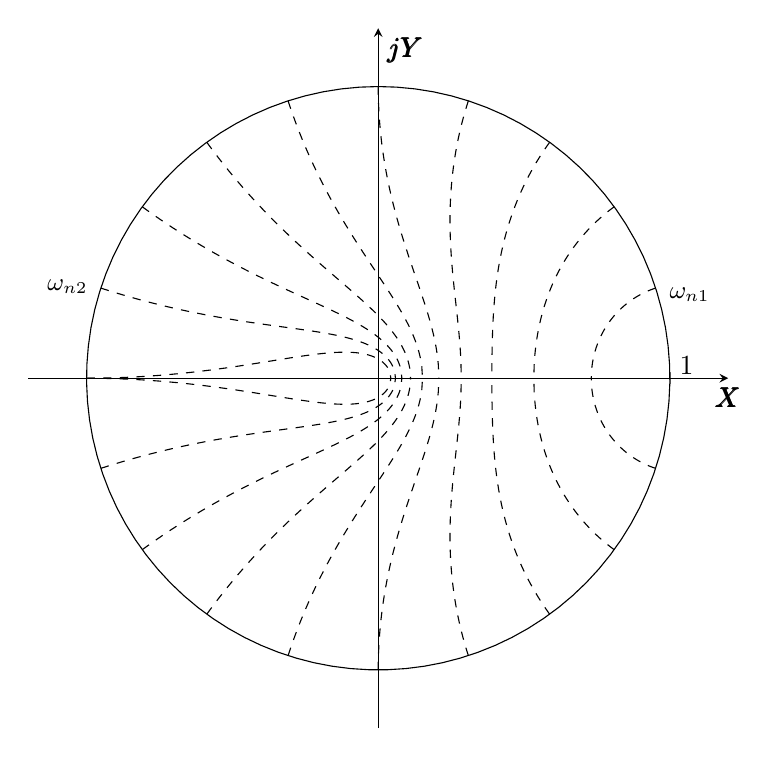
\begin{tikzpicture}

\begin{axis}[%
  axis lines=center,
  width=3.5in,
  height=3.5in,
  scale only axis,
  xmin=-1.2,
  xmax=1.2,
  ymin=-1.2,
  ymax=1.2,
  xtick={1},
  ytick=\empty,
  %xticklabels={},
  xticklabel style={anchor=south west},
  x label style={anchor=north},
  xlabel={$\pmb{X}$},
  ylabel={$\pmb{jY}$}
  ]
  \addplot [color=black, forget plot]
    table[row sep=crcr]{%
  0	1\\
  0.0634239196565645	0.997986676471884\\
  0.126592453573749	0.991954812830795\\
  0.18925124436041	0.981928697262707\\
  0.251147987181079	0.967948701396356\\
  0.312033445698487	0.950071117740945\\
  0.371662455660328	0.928367933016073\\
  0.429794912089172	0.902926538286621\\
  0.486196736100469	0.873849377069785\\
  0.540640817455598	0.841253532831181\\
  0.59290792905464	0.805270257531059\\
  0.642787609686539	0.766044443118978\\
  0.690079011482112	0.72373403810507\\
  0.734591708657533	0.678509411557132\\
  0.776146464291757	0.630552667084523\\
  0.814575952050336	0.580056909571198\\
  0.849725429949514	0.527225467610502\\
  0.881453363447582	0.472271074772683\\
  0.909631995354518	0.415415013001886\\
  0.934147860265107	0.356886221591872\\
  0.954902241444074	0.296920375328275\\
  0.971811568323542	0.235758935509427\\
  0.984807753012208	0.173648177666931\\
  0.993838464461254	0.110838199901011\\
  0.998867339183008	0.0475819158237424\\
  0.999874127673875	-0.015865963834808\\
  0.996854775951942	-0.0792499568567885\\
  0.989821441880933	-0.142314838273285\\
  0.978802446214779	-0.204806668065191\\
  0.963842158559942	-0.266473813690035\\
  0.945000818714669	-0.327067963317421\\
  0.922354294104581	-0.386345125693128\\
  0.895993774291336	-0.444066612605774\\
  0.866025403784439	-0.5\\
  0.832569854634771	-0.55392006386611\\
  0.795761840530832	-0.605609687137666\\
  0.755749574354258	-0.654860733945285\\
  0.712694171378863	-0.701474887706321\\
  0.666769000516292	-0.745264449675755\\
  0.618158986220605	-0.786053094742787\\
  0.567059863862771	-0.823676581429833\\
  0.513677391573407	-0.857983413234977\\
  0.458226521727411	-0.888835448654923\\
  0.400930535406614	-0.916108457432069\\
  0.342020143325669	-0.939692620785908\\
  0.28173255684143	-0.959492973614497\\
  0.220310532786541	-0.975429786885407\\
  0.15800139597335	-0.987438888676394\\
  0.0950560433041829	-0.995471922573085\\
  0.0317279334980681	-0.999496542383185\\
  -0.0317279334980679	-0.999496542383185\\
  -0.0950560433041826	-0.995471922573085\\
  -0.15800139597335	-0.987438888676394\\
  -0.220310532786541	-0.975429786885407\\
  -0.281732556841429	-0.959492973614497\\
  -0.342020143325669	-0.939692620785908\\
  -0.400930535406613	-0.91610845743207\\
  -0.45822652172741	-0.888835448654924\\
  -0.513677391573406	-0.857983413234977\\
  -0.567059863862771	-0.823676581429833\\
  -0.618158986220605	-0.786053094742788\\
  -0.666769000516292	-0.745264449675755\\
  -0.712694171378863	-0.701474887706322\\
  -0.755749574354258	-0.654860733945285\\
  -0.795761840530832	-0.605609687137667\\
  -0.832569854634771	-0.55392006386611\\
  -0.866025403784438	-0.5\\
  -0.895993774291336	-0.444066612605774\\
  -0.922354294104581	-0.386345125693129\\
  -0.945000818714668	-0.327067963317422\\
  -0.963842158559942	-0.266473813690035\\
  -0.978802446214779	-0.204806668065191\\
  -0.989821441880933	-0.142314838273285\\
  -0.996854775951942	-0.0792499568567888\\
  -0.999874127673875	-0.0158659638348076\\
  -0.998867339183008	0.0475819158237424\\
  -0.993838464461254	0.110838199901011\\
  -0.984807753012208	0.17364817766693\\
  -0.971811568323542	0.235758935509427\\
  -0.954902241444074	0.296920375328275\\
  -0.934147860265107	0.356886221591872\\
  -0.909631995354519	0.415415013001886\\
  -0.881453363447582	0.472271074772682\\
  -0.849725429949514	0.527225467610502\\
  -0.814575952050336	0.580056909571198\\
  -0.776146464291757	0.630552667084522\\
  -0.734591708657534	0.678509411557132\\
  -0.690079011482113	0.723734038105069\\
  -0.64278760968654	0.766044443118977\\
  -0.59290792905464	0.805270257531059\\
  -0.540640817455597	0.841253532831181\\
  -0.486196736100469	0.873849377069785\\
  -0.429794912089172	0.902926538286621\\
  -0.371662455660328	0.928367933016072\\
  -0.312033445698487	0.950071117740945\\
  -0.251147987181079	0.967948701396356\\
  -0.189251244360411	0.981928697262707\\
  -0.12659245357375	0.991954812830795\\
  -0.0634239196565654	0.997986676471884\\
  -2.44929359829471e-16	1\\
  };
  \addplot [color=black, dashed, forget plot]
    table[row sep=crcr]{%
  1	0\\
  1	0\\
  1	0\\
  1	0\\
  1	0\\
  1	0\\
  1	0\\
  1	0\\
  1	0\\
  1	0\\
  1	0\\
  1	0\\
  1	0\\
  1	0\\
  1	0\\
  1	0\\
  1	0\\
  1	0\\
  1	0\\
  1	0\\
  1	0\\
  1	0\\
  1	0\\
  1	0\\
  1	0\\
  1	0\\
  1	0\\
  1	0\\
  1	0\\
  1	0\\
  1	0\\
  1	0\\
  1	0\\
  1	0\\
  1	0\\
  1	0\\
  1	0\\
  1	0\\
  1	0\\
  1	0\\
  1	0\\
  1	0\\
  1	0\\
  1	0\\
  1	0\\
  1	0\\
  1	0\\
  1	0\\
  1	0\\
  1	0\\
  1	0\\
  1	0\\
  1	0\\
  1	0\\
  1	0\\
  1	0\\
  1	0\\
  1	0\\
  1	0\\
  1	0\\
  1	0\\
  1	0\\
  1	0\\
  1	0\\
  1	0\\
  1	0\\
  1	0\\
  1	0\\
  1	0\\
  1	0\\
  1	0\\
  1	0\\
  1	0\\
  1	0\\
  1	0\\
  1	0\\
  1	0\\
  1	0\\
  1	0\\
  1	0\\
  1	0\\
  1	0\\
  1	0\\
  1	0\\
  1	0\\
  1	0\\
  1	0\\
  1	0\\
  1	0\\
  1	0\\
  1	0\\
  1	0\\
  1	0\\
  1	0\\
  1	0\\
  1	0\\
  1	0\\
  1	0\\
  1	0\\
  1	0\\
  1	0\\
  };
  \addplot [color=black, dashed, forget plot]
    table[row sep=crcr]{%
  1	-0\\
  1	-0\\
  1	-0\\
  1	-0\\
  1	-0\\
  1	-0\\
  1	-0\\
  1	-0\\
  1	-0\\
  1	-0\\
  1	-0\\
  1	-0\\
  1	-0\\
  1	-0\\
  1	-0\\
  1	-0\\
  1	-0\\
  1	-0\\
  1	-0\\
  1	-0\\
  1	-0\\
  1	-0\\
  1	-0\\
  1	-0\\
  1	-0\\
  1	-0\\
  1	-0\\
  1	-0\\
  1	-0\\
  1	-0\\
  1	-0\\
  1	-0\\
  1	-0\\
  1	-0\\
  1	-0\\
  1	-0\\
  1	-0\\
  1	-0\\
  1	-0\\
  1	-0\\
  1	-0\\
  1	-0\\
  1	-0\\
  1	-0\\
  1	-0\\
  1	-0\\
  1	-0\\
  1	-0\\
  1	-0\\
  1	-0\\
  1	-0\\
  1	-0\\
  1	-0\\
  1	-0\\
  1	-0\\
  1	-0\\
  1	-0\\
  1	-0\\
  1	-0\\
  1	-0\\
  1	-0\\
  1	-0\\
  1	-0\\
  1	-0\\
  1	-0\\
  1	-0\\
  1	-0\\
  1	-0\\
  1	-0\\
  1	-0\\
  1	-0\\
  1	-0\\
  1	-0\\
  1	-0\\
  1	-0\\
  1	-0\\
  1	-0\\
  1	-0\\
  1	-0\\
  1	-0\\
  1	-0\\
  1	-0\\
  1	-0\\
  1	-0\\
  1	-0\\
  1	-0\\
  1	-0\\
  1	-0\\
  1	-0\\
  1	-0\\
  1	-0\\
  1	-0\\
  1	-0\\
  1	-0\\
  1	-0\\
  1	-0\\
  1	-0\\
  1	-0\\
  1	-0\\
  1	-0\\
  1	-0\\
  };
  \addplot [color=black, dashed, forget plot]
    table[row sep=crcr]{%
  0.951056516295154	0.309016994374947\\
  0.948078211301426	0.308032819485629\\
  0.94511888037394	0.307022081427976\\
  0.94217840366768	0.305985034984172\\
  0.939256662092049	0.30492192361348\\
  0.936353537306121	0.303832979577804\\
  0.933468911713929	0.302718424052102\\
  0.930602668459788	0.301578467219792\\
  0.927754691423642	0.30041330835324\\
  0.924924865216435	0.299223135879386\\
  0.922113075175525	0.298008127430492\\
  0.919319207360115	0.296768449879946\\
  0.916543148546715	0.295504259363022\\
  0.913784786224637	0.294215701282409\\
  0.911044008591513	0.292902910298318\\
  0.908320704548844	0.29156601030284\\
  0.905614763697579	0.29020511437826\\
  0.902926076333714	0.288820324738888\\
  0.900254533443929	0.287411732655945\\
  0.897600026701241	0.28597941836497\\
  0.894962448460698	0.284523450955115\\
  0.892341691755087	0.283043888239634\\
  0.889737650290675	0.281540776606779\\
  0.887150218442978	0.280014150850231\\
  0.884579291252554	0.278464033978077\\
  0.882024764420821	0.276890436999237\\
  0.879486534305908	0.275293358686166\\
  0.876964497918523	0.273672785312444\\
  0.874458552917854	0.272028690363831\\
  0.871968597607491	0.270361034221102\\
  0.869494530931379	0.268669763812905\\
  0.867036252469787	0.266954812236614\\
  0.864593662435318	0.265216098345006\\
  0.862166661668925	0.26345352629632\\
  0.859755151635967	0.261666985065034\\
  0.857359034422282	0.259856347910378\\
  0.85497821273029	0.258021471799335\\
  0.852612589875111	0.256162196780482\\
  0.850262069780723	0.25427834530468\\
  0.847926556976125	0.252369721488147\\
  0.845605956591542	0.250436110312975\\
  0.843300174354642	0.248477276759611\\
  0.84100911658678	0.246492964865175\\
  0.838732690199269	0.244482896700812\\
  0.836470802689669	0.24244677126046\\
  0.834223362138104	0.240384263252536\\
  0.831990277203598	0.238295021785015\\
  0.829771457120436	0.236178668933188\\
  0.82756681169455	0.234034798178102\\
  0.825376251299925	0.231862972702111\\
  0.823199686875027	0.22966272352627\\
  0.821037029919253	0.227433547472237\\
  0.818888192489409	0.225174904929094\\
  0.816753087196205	0.222886217402748\\
  0.814631627200769	0.22056686482251\\
  0.812523726211192	0.218216182575799\\
  0.810429298479085	0.215833458237678\\
  0.808348258796166	0.213417927956994\\
  0.806280522490864	0.210968772455044\\
  0.804226005424942	0.20848511258581\\
  0.802184623990148	0.205966004398664\\
  0.800156295104881	0.203410433634767\\
  0.798140936210878	0.200817309576802\\
  0.79613846526993	0.198185458157835\\
  0.794148800760608	0.195513614218404\\
  0.792171861675014	0.192800412780721\\
  0.790207567515554	0.190044379184321\\
  0.788255838291729	0.187243917897442\\
  0.78631659451695	0.184397299781511\\
  0.784389757205364	0.181502647540445\\
  0.78247524786871	0.178557919029679\\
  0.78057298851319	0.175560888028661\\
  0.778682901636361	0.172509121990832\\
  0.776804910224043	0.169399956171062\\
  0.774938937747252	0.166230463384427\\
  0.773084908159148	0.162997418461557\\
  0.771242745892004	0.159697256219759\\
  0.769412375854194	0.156326021445345\\
  0.7675937234272	0.15287930895176\\
  0.765786714462635	0.14935219119843\\
  0.763991275279289	0.145739130165498\\
  0.762207332660193	0.142033869089184\\
  0.760434813849697	0.138229298134639\\
  0.75867364655057	0.134317285907685\\
  0.756923758921121	0.130288465553936\\
  0.755185079572328	0.126131959533784\\
  0.753457537565001	0.121835020122195\\
  0.751741062406945	0.117382551784649\\
  0.750035584050153	0.11275646423786\\
  0.748341032888014	0.107934776522348\\
  0.746657339752536	0.102890343917207\\
  0.744984435911586	0.0975889934047091\\
  0.743322253066156	0.0919866926847057\\
  0.741670723347631	0.0860250595183118\\
  0.740029779315089	0.0796238406412504\\
  0.738399353952608	0.0726674092994395\\
  0.736779380666597	0.0649781812312819\\
  0.735169793283135	0.0562570328679831\\
  0.733570526045337	0.0459203986166819\\
  0.73198151361073	0.0324609316188515\\
  0.730402691048646	0\\
  };
  \addplot [color=black, dashed, forget plot]
    table[row sep=crcr]{%
  0.951056516295154	-0.309016994374947\\
  0.948078211301426	-0.308032819485629\\
  0.94511888037394	-0.307022081427976\\
  0.94217840366768	-0.305985034984172\\
  0.939256662092049	-0.30492192361348\\
  0.936353537306121	-0.303832979577804\\
  0.933468911713929	-0.302718424052102\\
  0.930602668459788	-0.301578467219792\\
  0.927754691423642	-0.30041330835324\\
  0.924924865216435	-0.299223135879386\\
  0.922113075175525	-0.298008127430492\\
  0.919319207360115	-0.296768449879946\\
  0.916543148546715	-0.295504259363022\\
  0.913784786224637	-0.294215701282409\\
  0.911044008591513	-0.292902910298318\\
  0.908320704548844	-0.29156601030284\\
  0.905614763697579	-0.29020511437826\\
  0.902926076333714	-0.288820324738888\\
  0.900254533443929	-0.287411732655945\\
  0.897600026701241	-0.28597941836497\\
  0.894962448460698	-0.284523450955115\\
  0.892341691755087	-0.283043888239634\\
  0.889737650290675	-0.281540776606779\\
  0.887150218442978	-0.280014150850231\\
  0.884579291252554	-0.278464033978077\\
  0.882024764420821	-0.276890436999237\\
  0.879486534305908	-0.275293358686166\\
  0.876964497918523	-0.273672785312444\\
  0.874458552917854	-0.272028690363831\\
  0.871968597607491	-0.270361034221102\\
  0.869494530931379	-0.268669763812905\\
  0.867036252469787	-0.266954812236614\\
  0.864593662435318	-0.265216098345006\\
  0.862166661668925	-0.26345352629632\\
  0.859755151635967	-0.261666985065034\\
  0.857359034422282	-0.259856347910378\\
  0.85497821273029	-0.258021471799335\\
  0.852612589875111	-0.256162196780482\\
  0.850262069780723	-0.25427834530468\\
  0.847926556976125	-0.252369721488147\\
  0.845605956591542	-0.250436110312975\\
  0.843300174354642	-0.248477276759611\\
  0.84100911658678	-0.246492964865175\\
  0.838732690199269	-0.244482896700812\\
  0.836470802689669	-0.24244677126046\\
  0.834223362138104	-0.240384263252536\\
  0.831990277203598	-0.238295021785015\\
  0.829771457120436	-0.236178668933188\\
  0.82756681169455	-0.234034798178102\\
  0.825376251299925	-0.231862972702111\\
  0.823199686875027	-0.22966272352627\\
  0.821037029919253	-0.227433547472237\\
  0.818888192489409	-0.225174904929094\\
  0.816753087196205	-0.222886217402748\\
  0.814631627200769	-0.22056686482251\\
  0.812523726211192	-0.218216182575799\\
  0.810429298479085	-0.215833458237678\\
  0.808348258796166	-0.213417927956994\\
  0.806280522490864	-0.210968772455044\\
  0.804226005424942	-0.20848511258581\\
  0.802184623990148	-0.205966004398664\\
  0.800156295104881	-0.203410433634767\\
  0.798140936210878	-0.200817309576802\\
  0.79613846526993	-0.198185458157835\\
  0.794148800760608	-0.195513614218404\\
  0.792171861675014	-0.192800412780721\\
  0.790207567515554	-0.190044379184321\\
  0.788255838291729	-0.187243917897442\\
  0.78631659451695	-0.184397299781511\\
  0.784389757205364	-0.181502647540445\\
  0.78247524786871	-0.178557919029679\\
  0.78057298851319	-0.175560888028661\\
  0.778682901636361	-0.172509121990832\\
  0.776804910224043	-0.169399956171062\\
  0.774938937747252	-0.166230463384427\\
  0.773084908159148	-0.162997418461557\\
  0.771242745892004	-0.159697256219759\\
  0.769412375854194	-0.156326021445345\\
  0.7675937234272	-0.15287930895176\\
  0.765786714462635	-0.14935219119843\\
  0.763991275279289	-0.145739130165498\\
  0.762207332660193	-0.142033869089184\\
  0.760434813849697	-0.138229298134639\\
  0.75867364655057	-0.134317285907685\\
  0.756923758921121	-0.130288465553936\\
  0.755185079572328	-0.126131959533784\\
  0.753457537565001	-0.121835020122195\\
  0.751741062406945	-0.117382551784649\\
  0.750035584050153	-0.11275646423786\\
  0.748341032888014	-0.107934776522348\\
  0.746657339752536	-0.102890343917207\\
  0.744984435911586	-0.0975889934047091\\
  0.743322253066156	-0.0919866926847057\\
  0.741670723347631	-0.0860250595183118\\
  0.740029779315089	-0.0796238406412504\\
  0.738399353952608	-0.0726674092994395\\
  0.736779380666597	-0.0649781812312819\\
  0.735169793283135	-0.0562570328679831\\
  0.733570526045337	-0.0459203986166819\\
  0.73198151361073	-0.0324609316188515\\
  0.730402691048646	-0\\
  };
  \addplot [color=black, dashed, forget plot]
    table[row sep=crcr]{%
  0.809016994374947	0.587785252292473\\
  0.803968076864246	0.584078409040141\\
  0.798987139554922	0.580344731698571\\
  0.794073302703513	0.576584983615173\\
  0.789225697784154	0.572799896343767\\
  0.784443467346559	0.568990170355869\\
  0.779725764875798	0.565156475711343\\
  0.775071754653839	0.561299452689503\\
  0.770480611622838	0.55741971238163\\
  0.765951521250147	0.55351783724576\\
  0.761483679395036	0.549594381624462\\
  0.757076292177084	0.545649872226245\\
  0.752728575846238	0.541684808571098\\
  0.748439756654506	0.537699663400556\\
  0.744209070729268	0.533694883052599\\
  0.740035763948193	0.529670887801542\\
  0.735919091815723	0.525628072162995\\
  0.73185831934112	0.521566805163826\\
  0.727852720918053	0.517487430576977\\
  0.723901580205702	0.513390267120805\\
  0.72000419001136	0.509275608622555\\
  0.716159852174521	0.505143724145385\\
  0.712367877452424	0.500994858078254\\
  0.708627585407048	0.496829230187816\\
  0.704938304293527	0.492647035631308\\
  0.701299370949976	0.488448444929261\\
  0.697710130688707	0.484233603896658\\
  0.694169937188816	0.480002633530983\\
  0.690678152390127	0.475755629855389\\
  0.687234146388471	0.471492663714971\\
  0.683837297332295	0.467213780523892\\
  0.680486991320567	0.462918999960819\\
  0.677182622301969	0.458608315609828\\
  0.673923591975373	0.45428169454361\\
  0.67070930969156	0.449939076845429\\
  0.667539192356189	0.445580375065885\\
  0.664412664333986	0.441205473610068\\
  0.661329157354143	0.436814228050209\\
  0.658288110416912	0.43240646435835\\
  0.655288969701381	0.427981978052936\\
  0.652331188474404	0.423540533252536\\
  0.649414227000697	0.419081861629092\\
  0.646537552454051	0.414605661252235\\
  0.643700638829683	0.410111595315165\\
  0.640902966857678	0.405599290731511\\
  0.638144023917538	0.401068336591244\\
  0.635423303953798	0.396518282462304\\
  0.632740307392718	0.391948636522913\\
  0.630094541060018	0.387358863507658\\
  0.627485518099657	0.382748382448251\\
  0.624912757893638	0.378116564187382\\
  0.622375785982821	0.37346272864121\\
  0.619874133988746	0.368786141782721\\
  0.617407339536427	0.364086012314358\\
  0.614974946178141	0.359361487993868\\
  0.612576503318165	0.35461165157214\\
  0.610211566138466	0.349835516295752\\
  0.607879695525337	0.345032020919843\\
  0.605580457996952	0.340200024168619\\
  0.603313425631842	0.335338298570911\\
  0.601078175998265	0.330445523586591\\
  0.598874292084485	0.325520277925745\\
  0.596701362229912	0.320561030945957\\
  0.594558980057129	0.315566132993194\\
  0.592446744404769	0.310533804527835\\
  0.590364259261241	0.305462123848429\\
  0.588311133699294	0.300349013190491\\
  0.586286981811413	0.295192222934552\\
  0.584291422646021	0.289989313604637\\
  0.582324080144498	0.284737635272761\\
  0.580384583078989	0.279434303903338\\
  0.578472564991001	0.274076174069122\\
  0.576587664130775	0.268659807341124\\
  0.574729523397425	0.263181435490837\\
  0.572897790279837	0.257636917432723\\
  0.571092116798306	0.252021688563062\\
  0.569312159446919	0.246330700796692\\
  0.567557579136666	0.240558351136193\\
  0.565828041139265	0.234698395986517\\
  0.564123215031705	0.228743847591282\\
  0.562442774641479	0.222686847826466\\
  0.560786397992523	0.216518513011748\\
  0.559153767251828	0.210228741191177\\
  0.557544568676733	0.203805970188717\\
  0.555958492562879	0.1972368701823\\
  0.554395233192832	0.190505947794269\\
  0.55285448878534	0.183595028500902\\
  0.551335961445247	0.17648256837326\\
  0.549839357114031	0.169142721020148\\
  0.548364385520971	0.161544044294541\\
  0.546910760134932	0.15364766095089\\
  0.54547819811676	0.145404562405573\\
  0.544066420272276	0.136751511316999\\
  0.542675151005869	0.127604536237939\\
  0.541304118274676	0.117848026435929\\
  0.539953053543337	0.107315136160232\\
  0.538621691739329	0.0957491682488516\\
  0.537309771208858	0.0827169424485554\\
  0.536017033673318	0.0673717019389019\\
  0.534743224186292	0.0475216037191627\\
  0.533488091091103	0\\
  };
  \addplot [color=black, dashed, forget plot]
    table[row sep=crcr]{%
  0.809016994374947	-0.587785252292473\\
  0.803968076864246	-0.584078409040141\\
  0.798987139554922	-0.580344731698571\\
  0.794073302703513	-0.576584983615173\\
  0.789225697784154	-0.572799896343767\\
  0.784443467346559	-0.568990170355869\\
  0.779725764875798	-0.565156475711343\\
  0.775071754653839	-0.561299452689503\\
  0.770480611622838	-0.55741971238163\\
  0.765951521250147	-0.55351783724576\\
  0.761483679395036	-0.549594381624462\\
  0.757076292177084	-0.545649872226245\\
  0.752728575846238	-0.541684808571098\\
  0.748439756654506	-0.537699663400556\\
  0.744209070729268	-0.533694883052599\\
  0.740035763948193	-0.529670887801542\\
  0.735919091815723	-0.525628072162995\\
  0.73185831934112	-0.521566805163826\\
  0.727852720918053	-0.517487430576977\\
  0.723901580205702	-0.513390267120805\\
  0.72000419001136	-0.509275608622555\\
  0.716159852174521	-0.505143724145385\\
  0.712367877452424	-0.500994858078254\\
  0.708627585407048	-0.496829230187816\\
  0.704938304293527	-0.492647035631308\\
  0.701299370949976	-0.488448444929261\\
  0.697710130688707	-0.484233603896658\\
  0.694169937188816	-0.480002633530983\\
  0.690678152390127	-0.475755629855389\\
  0.687234146388471	-0.471492663714971\\
  0.683837297332295	-0.467213780523892\\
  0.680486991320567	-0.462918999960819\\
  0.677182622301969	-0.458608315609828\\
  0.673923591975373	-0.45428169454361\\
  0.67070930969156	-0.449939076845429\\
  0.667539192356189	-0.445580375065885\\
  0.664412664333986	-0.441205473610068\\
  0.661329157354143	-0.436814228050209\\
  0.658288110416912	-0.43240646435835\\
  0.655288969701381	-0.427981978052936\\
  0.652331188474404	-0.423540533252536\\
  0.649414227000697	-0.419081861629092\\
  0.646537552454051	-0.414605661252235\\
  0.643700638829683	-0.410111595315165\\
  0.640902966857678	-0.405599290731511\\
  0.638144023917538	-0.401068336591244\\
  0.635423303953798	-0.396518282462304\\
  0.632740307392718	-0.391948636522913\\
  0.630094541060018	-0.387358863507658\\
  0.627485518099657	-0.382748382448251\\
  0.624912757893638	-0.378116564187382\\
  0.622375785982821	-0.37346272864121\\
  0.619874133988746	-0.368786141782721\\
  0.617407339536427	-0.364086012314358\\
  0.614974946178141	-0.359361487993868\\
  0.612576503318165	-0.35461165157214\\
  0.610211566138466	-0.349835516295752\\
  0.607879695525337	-0.345032020919843\\
  0.605580457996952	-0.340200024168619\\
  0.603313425631842	-0.335338298570911\\
  0.601078175998265	-0.330445523586591\\
  0.598874292084485	-0.325520277925745\\
  0.596701362229912	-0.320561030945957\\
  0.594558980057129	-0.315566132993194\\
  0.592446744404769	-0.310533804527835\\
  0.590364259261241	-0.305462123848429\\
  0.588311133699294	-0.300349013190491\\
  0.586286981811413	-0.295192222934552\\
  0.584291422646021	-0.289989313604637\\
  0.582324080144498	-0.284737635272761\\
  0.580384583078989	-0.279434303903338\\
  0.578472564991001	-0.274076174069122\\
  0.576587664130775	-0.268659807341124\\
  0.574729523397425	-0.263181435490837\\
  0.572897790279837	-0.257636917432723\\
  0.571092116798306	-0.252021688563062\\
  0.569312159446919	-0.246330700796692\\
  0.567557579136666	-0.240558351136193\\
  0.565828041139265	-0.234698395986517\\
  0.564123215031705	-0.228743847591282\\
  0.562442774641479	-0.222686847826466\\
  0.560786397992523	-0.216518513011748\\
  0.559153767251828	-0.210228741191177\\
  0.557544568676733	-0.203805970188717\\
  0.555958492562879	-0.1972368701823\\
  0.554395233192832	-0.190505947794269\\
  0.55285448878534	-0.183595028500902\\
  0.551335961445247	-0.17648256837326\\
  0.549839357114031	-0.169142721020148\\
  0.548364385520971	-0.161544044294541\\
  0.546910760134932	-0.15364766095089\\
  0.54547819811676	-0.145404562405573\\
  0.544066420272276	-0.136751511316999\\
  0.542675151005869	-0.127604536237939\\
  0.541304118274676	-0.117848026435929\\
  0.539953053543337	-0.107315136160232\\
  0.538621691739329	-0.0957491682488516\\
  0.537309771208858	-0.0827169424485554\\
  0.536017033673318	-0.0673717019389019\\
  0.534743224186292	-0.0475216037191627\\
  0.533488091091103	-0\\
  };
  \addplot [color=black, dashed, forget plot]
    table[row sep=crcr]{%
  0.587785252292473	0.809016994374947\\
  0.582309297119587	0.801400566795492\\
  0.576959183297469	0.793801457674205\\
  0.571732340353481	0.786220466749031\\
  0.56662624829927	0.778658336620054\\
  0.561638436656923	0.771115754699379\\
  0.556766483503744	0.763593355066369\\
  0.552008014535265	0.75609172023173\\
  0.547360702146168	0.748611382813718\\
  0.542822264528764	0.741152827129482\\
  0.538390464788706	0.733716490704319\\
  0.534063110077599	0.726302765701431\\
  0.529838050742194	0.718912000274504\\
  0.525713179489847	0.711544499845278\\
  0.52168643056993	0.704200528308028\\
  0.517755778970906	0.696880309162698\\
  0.513919239632746	0.689584026578232\\
  0.510174866674423	0.682311826387443\\
  0.506520752636174	0.675063817014576\\
  0.502955027736264	0.667840070336502\\
  0.499475859141973	0.660640622478329\\
  0.496081450254526	0.653465474543956\\
  0.492770040007721	0.646314593281934\\
  0.489539902179967	0.639187911686782\\
  0.48638934471951	0.632085329535654\\
  0.483316709082561	0.625006713860077\\
  0.480320369584116	0.61795189935219\\
  0.477398732761191	0.610920688704696\\
  0.474550236748266	0.603912852883462\\
  0.471773350664695	0.596928131331407\\
  0.469066574013837	0.589966232102021\\
  0.466428436093723	0.583026831920531\\
  0.463857495418998	0.576109576170361\\
  0.461352339153956	0.569214078802161\\
  0.458911582556433	0.56233992216223\\
  0.456533868432375	0.555486656736729\\
  0.454217866600849	0.548653800807529\\
  0.451962273369329	0.541840840015008\\
  0.449765811019036	0.535047226822452\\
  0.447627227300158	0.528272379876049\\
  0.445545294936748	0.521515683253672\\
  0.443518811141127	0.514776485594762\\
  0.441546597137611	0.508054099102692\\
  0.439627497695365	0.501347798409846\\
  0.437760380670245	0.494656819294441\\
  0.435944136555421	0.487980357236711\\
  0.434177678040635	0.481317565800483\\
  0.432459939579929	0.474667554824374\\
  0.430789876967667	0.468029388404762\\
  0.42916646692271	0.461402082650359\\
  0.427588706680582	0.454784603185479\\
  0.426055613593464	0.448175862376014\\
  0.42456622473789	0.441574716248516\\
  0.423119596529975	0.434979961068675\\
  0.421714804348045	0.428390329540639\\
  0.420350942162526	0.421804486583022\\
  0.419027122172945	0.415221024630929\\
  0.417742474451922	0.408638458405624\\
  0.41649614659601	0.402055219084459\\
  0.415287303383244	0.395469647793065\\
  0.414115126437298	0.388879988329137\\
  0.412978813898094	0.382284379012195\\
  0.411877580098755	0.375680843535754\\
  0.410810655248786	0.369067280676845\\
  0.409777285123346	0.362441452691912\\
  0.408776730758515	0.355800972196766\\
  0.407808268152427	0.349143287290061\\
  0.406871187972163	0.342465664633109\\
  0.405964795266295	0.33576517014133\\
  0.405088409182968	0.329038646871611\\
  0.404241362693423	0.322282689601277\\
  0.403423002320843	0.315493615483433\\
  0.40263268787444	0.308667430023397\\
  0.401869792188659	0.301799787442834\\
  0.401133700867428	0.294885944269923\\
  0.40042381203333	0.287920704698758\\
  0.399739536081626	0.280898355876161\\
  0.399080295439023	0.273812590766852\\
  0.398445524327102	0.266656415572581\\
  0.39783466853031	0.259422037771358\\
  0.39724718516844	0.252100729602985\\
  0.396682542473503	0.244682660113701\\
  0.396140219570916	0.237156686470128\\
  0.395619706264911	0.229510091829081\\
  0.395120502828102	0.22172825208392\\
  0.394642119795116	0.213794206462818\\
  0.394184077760218	0.205688095849274\\
  0.393745907178842	0.197386415490307\\
  0.39332714817298	0.188861001355175\\
  0.392927350340317	0.180077624368305\\
  0.392546072567074	0.170993989987095\\
  0.392182882844471	0.161556804181116\\
  0.39183735808874	0.151697312104007\\
  0.391509083964633	0.14132421085842\\
  0.391197654712337	0.130311761848054\\
  0.390902672977758	0.118478416754367\\
  0.390623749646079	0.105544670782668\\
  0.390360503678557	0.0910384509401026\\
  0.390112561952479	0.0740360106835001\\
  0.389879559104218	0.0521431986535175\\
  0.389661137375347	0\\
  };
  \addplot [color=black, dashed, forget plot]
    table[row sep=crcr]{%
  0.587785252292473	-0.809016994374947\\
  0.582309297119587	-0.801400566795492\\
  0.576959183297469	-0.793801457674205\\
  0.571732340353481	-0.786220466749031\\
  0.56662624829927	-0.778658336620054\\
  0.561638436656923	-0.771115754699379\\
  0.556766483503744	-0.763593355066369\\
  0.552008014535265	-0.75609172023173\\
  0.547360702146168	-0.748611382813718\\
  0.542822264528764	-0.741152827129482\\
  0.538390464788706	-0.733716490704319\\
  0.534063110077599	-0.726302765701431\\
  0.529838050742194	-0.718912000274504\\
  0.525713179489847	-0.711544499845278\\
  0.52168643056993	-0.704200528308028\\
  0.517755778970906	-0.696880309162698\\
  0.513919239632746	-0.689584026578232\\
  0.510174866674423	-0.682311826387443\\
  0.506520752636174	-0.675063817014576\\
  0.502955027736264	-0.667840070336502\\
  0.499475859141973	-0.660640622478329\\
  0.496081450254526	-0.653465474543956\\
  0.492770040007721	-0.646314593281934\\
  0.489539902179967	-0.639187911686782\\
  0.48638934471951	-0.632085329535654\\
  0.483316709082561	-0.625006713860077\\
  0.480320369584116	-0.61795189935219\\
  0.477398732761191	-0.610920688704696\\
  0.474550236748266	-0.603912852883462\\
  0.471773350664695	-0.596928131331407\\
  0.469066574013837	-0.589966232102021\\
  0.466428436093723	-0.583026831920531\\
  0.463857495418998	-0.576109576170361\\
  0.461352339153956	-0.569214078802161\\
  0.458911582556433	-0.56233992216223\\
  0.456533868432375	-0.555486656736729\\
  0.454217866600849	-0.548653800807529\\
  0.451962273369329	-0.541840840015008\\
  0.449765811019036	-0.535047226822452\\
  0.447627227300158	-0.528272379876049\\
  0.445545294936748	-0.521515683253672\\
  0.443518811141127	-0.514776485594762\\
  0.441546597137611	-0.508054099102692\\
  0.439627497695365	-0.501347798409846\\
  0.437760380670245	-0.494656819294441\\
  0.435944136555421	-0.487980357236711\\
  0.434177678040635	-0.481317565800483\\
  0.432459939579929	-0.474667554824374\\
  0.430789876967667	-0.468029388404762\\
  0.42916646692271	-0.461402082650359\\
  0.427588706680582	-0.454784603185479\\
  0.426055613593464	-0.448175862376014\\
  0.42456622473789	-0.441574716248516\\
  0.423119596529975	-0.434979961068675\\
  0.421714804348045	-0.428390329540639\\
  0.420350942162526	-0.421804486583022\\
  0.419027122172945	-0.415221024630929\\
  0.417742474451922	-0.408638458405624\\
  0.41649614659601	-0.402055219084459\\
  0.415287303383244	-0.395469647793065\\
  0.414115126437298	-0.388879988329137\\
  0.412978813898094	-0.382284379012195\\
  0.411877580098755	-0.375680843535754\\
  0.410810655248786	-0.369067280676845\\
  0.409777285123346	-0.362441452691912\\
  0.408776730758515	-0.355800972196766\\
  0.407808268152427	-0.349143287290061\\
  0.406871187972163	-0.342465664633109\\
  0.405964795266295	-0.33576517014133\\
  0.405088409182968	-0.329038646871611\\
  0.404241362693423	-0.322282689601277\\
  0.403423002320843	-0.315493615483433\\
  0.40263268787444	-0.308667430023397\\
  0.401869792188659	-0.301799787442834\\
  0.401133700867428	-0.294885944269923\\
  0.40042381203333	-0.287920704698758\\
  0.399739536081626	-0.280898355876161\\
  0.399080295439023	-0.273812590766852\\
  0.398445524327102	-0.266656415572581\\
  0.39783466853031	-0.259422037771358\\
  0.39724718516844	-0.252100729602985\\
  0.396682542473503	-0.244682660113701\\
  0.396140219570916	-0.237156686470128\\
  0.395619706264911	-0.229510091829081\\
  0.395120502828102	-0.22172825208392\\
  0.394642119795116	-0.213794206462818\\
  0.394184077760218	-0.205688095849274\\
  0.393745907178842	-0.197386415490307\\
  0.39332714817298	-0.188861001355175\\
  0.392927350340317	-0.180077624368305\\
  0.392546072567074	-0.170993989987095\\
  0.392182882844471	-0.161556804181116\\
  0.39183735808874	-0.151697312104007\\
  0.391509083964633	-0.14132421085842\\
  0.391197654712337	-0.130311761848054\\
  0.390902672977758	-0.118478416754367\\
  0.390623749646079	-0.105544670782668\\
  0.390360503678557	-0.0910384509401026\\
  0.390112561952479	-0.0740360106835001\\
  0.389879559104218	-0.0521431986535175\\
  0.389661137375347	-0\\
  };
  \addplot [color=black, dashed, forget plot]
    table[row sep=crcr]{%
  0.309016994374947	0.951056516295154\\
  0.305217080709932	0.939160790507861\\
  0.30158044156387	0.92737595427122\\
  0.298102166735956	0.915701484457103\\
  0.294777480791454	0.904136795765201\\
  0.29160173950109	0.892681244240134\\
  0.288570426372682	0.881334130597075\\
  0.285679149272646	0.870094703364585\\
  0.282923637135083	0.858962161852849\\
  0.280299736756191	0.847935658954962\\
  0.277803409671828	0.837014303788469\\
  0.275430729116085	0.826197164183891\\
  0.273177877058799	0.81548326902653\\
  0.271041141319984	0.804871610457444\\
  0.269016912759193	0.794361145939081\\
  0.267101682537912	0.783950800190664\\
  0.265292039453092	0.77363946699808\\
  0.263584667340008	0.763426010902631\\
  0.261976342542652	0.75330926877269\\
  0.260463931449941	0.743288051261957\\
  0.259044388096041	0.733361144157651\\
  0.257714751823163	0.723527309621692\\
  0.256472145005221	0.713785287327568\\
  0.255313770830805	0.704133795495268\\
  0.254236911143918	0.694571531826333\\
  0.253238924341019	0.68509717434077\\
  0.252317243322908	0.675709382117202\\
  0.251469373500046	0.666406795937338\\
  0.250692890849941	0.657188038835442\\
  0.249985440025252	0.648051716553169\\
  0.249344732511311	0.638996417899726\\
  0.248768544831792	0.630020715016927\\
  0.248254716801288	0.621123163548305\\
  0.247801149823575	0.612302302710977\\
  0.247405805234411	0.603556655268511\\
  0.247066702687698	0.594884727402498\\
  0.246781918583901	0.586285008480007\\
  0.246549584539641	0.57775597071349\\
  0.24636788589738	0.569296068709032\\
  0.246235060274193	0.560903738898134\\
  0.246149396148586	0.552577398847419\\
  0.246109231484407	0.54431544643974\\
  0.246112952390872	0.536116258919226\\
  0.246158991817792	0.527978191791664\\
  0.246245828285069	0.51989957757039\\
  0.2463719846456	0.5118787243565\\
  0.246536026880706	0.503913914240565\\
  0.246736562927261	0.49600340151133\\
  0.246972241535691	0.488145410654776\\
  0.247241751158043	0.480338134124693\\
  0.247543818865362	0.472579729863208\\
  0.247877209293596	0.464868318546725\\
  0.248240723617312	0.45720198052923\\
  0.248633198550478	0.449578752450869\\
  0.249053505373641	0.441996623475051\\
  0.249500548986788	0.434453531111882\\
  0.249973266987244	0.426947356579379\\
  0.250470628771945	0.419475919646492\\
  0.25099163466347	0.412036972893213\\
  0.251535315059195	0.404628195312739\\
  0.252100729602985	0.39724718516844\\
  0.252686966378838	0.389891452003851\\
  0.253293141125898	0.382558407686555\\
  0.253918396474296	0.375245356346011\\
  0.254561901201278	0.367949483040285\\
  0.25522284950708	0.360667840956287\\
  0.255900460310047	0.353397336911125\\
  0.256593976560494	0.346134714877\\
  0.257302664572823	0.338876537196393\\
  0.258025813375412	0.33161916308546\\
  0.258762734077829	0.324358723937813\\
  0.2595127592549	0.317091094833371\\
  0.260275242347213	0.309811861521285\\
  0.261049557077614	0.302516281973398\\
  0.261835096883284	0.295199241383432\\
  0.262631274362992	0.287855199201125\\
  0.263437520739125	0.280478126417275\\
  0.264253285334109	0.273061430823931\\
  0.265078035060854	0.265597867319157\\
  0.265911253926843	0.258079429443833\\
  0.266752442551518	0.250497217135365\\
  0.26760111769661	0.242841274021111\\
  0.268456811809085	0.235100385243312\\
  0.26931907257636	0.227261823485223\\
  0.27018746249348	0.219311026048744\\
  0.271061558441942	0.21123117870405\\
  0.271940951279852	0.203002671250792\\
  0.272825245443132	0.194602373024796\\
  0.273714058557471	0.186002649972472\\
  0.274607021060755	0.177170001168297\\
  0.27550377583569	0.168063118087211\\
  0.276403977852351	0.158630037397896\\
  0.277307293820405	0.148803810458127\\
  0.278213401850743	0.138495621943914\\
  0.279121991126281	0.127583244080622\\
  0.280032761581685	0.115890270922272\\
  0.28094542359179	0.10314515796966\\
  0.281859697668478	0.0888892428442591\\
  0.282775314165799	0.0722247596536262\\
  0.28369201299311	0.0508237111825767\\
  0.284609543336029	0\\
  };
  \addplot [color=black, dashed, forget plot]
    table[row sep=crcr]{%
  0.309016994374947	-0.951056516295154\\
  0.305217080709932	-0.939160790507861\\
  0.30158044156387	-0.92737595427122\\
  0.298102166735956	-0.915701484457103\\
  0.294777480791454	-0.904136795765201\\
  0.29160173950109	-0.892681244240134\\
  0.288570426372682	-0.881334130597075\\
  0.285679149272646	-0.870094703364585\\
  0.282923637135083	-0.858962161852849\\
  0.280299736756191	-0.847935658954962\\
  0.277803409671828	-0.837014303788469\\
  0.275430729116085	-0.826197164183891\\
  0.273177877058799	-0.81548326902653\\
  0.271041141319984	-0.804871610457444\\
  0.269016912759193	-0.794361145939081\\
  0.267101682537912	-0.783950800190664\\
  0.265292039453092	-0.77363946699808\\
  0.263584667340008	-0.763426010902631\\
  0.261976342542652	-0.75330926877269\\
  0.260463931449941	-0.743288051261957\\
  0.259044388096041	-0.733361144157651\\
  0.257714751823163	-0.723527309621692\\
  0.256472145005221	-0.713785287327568\\
  0.255313770830805	-0.704133795495268\\
  0.254236911143918	-0.694571531826333\\
  0.253238924341019	-0.68509717434077\\
  0.252317243322908	-0.675709382117202\\
  0.251469373500046	-0.666406795937338\\
  0.250692890849941	-0.657188038835442\\
  0.249985440025252	-0.648051716553169\\
  0.249344732511311	-0.638996417899726\\
  0.248768544831792	-0.630020715016927\\
  0.248254716801288	-0.621123163548305\\
  0.247801149823575	-0.612302302710977\\
  0.247405805234411	-0.603556655268511\\
  0.247066702687698	-0.594884727402498\\
  0.246781918583901	-0.586285008480007\\
  0.246549584539641	-0.57775597071349\\
  0.24636788589738	-0.569296068709032\\
  0.246235060274193	-0.560903738898134\\
  0.246149396148586	-0.552577398847419\\
  0.246109231484407	-0.54431544643974\\
  0.246112952390872	-0.536116258919226\\
  0.246158991817792	-0.527978191791664\\
  0.246245828285069	-0.51989957757039\\
  0.2463719846456	-0.5118787243565\\
  0.246536026880706	-0.503913914240565\\
  0.246736562927261	-0.49600340151133\\
  0.246972241535691	-0.488145410654776\\
  0.247241751158043	-0.480338134124693\\
  0.247543818865362	-0.472579729863208\\
  0.247877209293596	-0.464868318546725\\
  0.248240723617312	-0.45720198052923\\
  0.248633198550478	-0.449578752450869\\
  0.249053505373641	-0.441996623475051\\
  0.249500548986788	-0.434453531111882\\
  0.249973266987244	-0.426947356579379\\
  0.250470628771945	-0.419475919646492\\
  0.25099163466347	-0.412036972893213\\
  0.251535315059195	-0.404628195312739\\
  0.252100729602985	-0.39724718516844\\
  0.252686966378838	-0.389891452003851\\
  0.253293141125898	-0.382558407686555\\
  0.253918396474296	-0.375245356346011\\
  0.254561901201278	-0.367949483040285\\
  0.25522284950708	-0.360667840956287\\
  0.255900460310047	-0.353397336911125\\
  0.256593976560494	-0.346134714877\\
  0.257302664572823	-0.338876537196393\\
  0.258025813375412	-0.33161916308546\\
  0.258762734077829	-0.324358723937813\\
  0.2595127592549	-0.317091094833371\\
  0.260275242347213	-0.309811861521285\\
  0.261049557077614	-0.302516281973398\\
  0.261835096883284	-0.295199241383432\\
  0.262631274362992	-0.287855199201125\\
  0.263437520739125	-0.280478126417275\\
  0.264253285334109	-0.273061430823931\\
  0.265078035060854	-0.265597867319157\\
  0.265911253926843	-0.258079429443833\\
  0.266752442551518	-0.250497217135365\\
  0.26760111769661	-0.242841274021111\\
  0.268456811809085	-0.235100385243312\\
  0.26931907257636	-0.227261823485223\\
  0.27018746249348	-0.219311026048744\\
  0.271061558441942	-0.21123117870405\\
  0.271940951279852	-0.203002671250792\\
  0.272825245443132	-0.194602373024796\\
  0.273714058557471	-0.186002649972472\\
  0.274607021060755	-0.177170001168297\\
  0.27550377583569	-0.168063118087211\\
  0.276403977852351	-0.158630037397896\\
  0.277307293820405	-0.148803810458127\\
  0.278213401850743	-0.138495621943914\\
  0.279121991126281	-0.127583244080622\\
  0.280032761581685	-0.115890270922272\\
  0.28094542359179	-0.10314515796966\\
  0.281859697668478	-0.0888892428442591\\
  0.282775314165799	-0.0722247596536262\\
  0.28369201299311	-0.0508237111825767\\
  0.284609543336029	-0\\
  };
  \addplot [color=black, dashed, forget plot]
    table[row sep=crcr]{%
  6.12323399573677e-17	1\\
  7.7317687626911e-05	0.984414760315379\\
  0.000304473526916821	0.969072378473437\\
  0.000674472828493945	0.953968964779478\\
  0.00118058169363121	0.93910062534589\\
  0.00181631801576277	0.924463466093766\\
  0.00257544278125555	0.910053596444375\\
  0.00345195165969545	0.89586713271811\\
  0.00444006687424801	0.881900201257456\\
  0.00553422934296521	0.868148941289481\\
  0.00672909108219705	0.854609507542394\\
  0.00801950786355669	0.841278072629794\\
  0.00940053211615922	0.828150829215367\\
  0.0108674060661241	0.815223991969978\\
  0.0124155551055848	0.802493799332324\\
  0.0140405813837066	0.789956515083569\\
  0.0157382576124464	0.777608429745714\\
  0.0175045210800292	0.765445861812744\\
  0.0193354678653398	0.753465158822996\\
  0.0212273472466501	0.741662698280554\\
  0.0231765562983096	0.730034888432912\\
  0.0251796346692383	0.718578168911567\\
  0.0272332595372588	0.707289011241661\\
  0.0293342407334911	0.696163919226269\\
  0.0314795160312324	0.6851994292104\\
  0.0336661465939105	0.674392110229289\\
  0.0358913125768861	0.663738564045043\\
  0.0381523088780405	0.653235425075212\\
  0.0404465410322538	0.642879360216395\\
  0.0427715212450352	0.632667068565439\\
  0.0451248645607202	0.622595281040359\\
  0.047504285160798	0.612660759902559\\
  0.0499075927880797	0.602860298181422\\
  0.0523326892925488	0.593190719001822\\
  0.0547775652948822	0.583648874814551\\
  0.0572402969637477	0.574231646529053\\
  0.0597190429031189	0.564935942547281\\
  0.0622120411459684	0.555758697696827\\
  0.0647176062508154	0.546696872060768\\
  0.0672341264977229	0.537747449700946\\
  0.0697600611804469	0.528907437270577\\
  0.0722939379915487	0.520173862511203\\
  0.0748343504973857	0.511543772628016\\
  0.0773799556999937	0.503014232536533\\
  0.0799294716829765	0.494582322972397\\
  0.0824816753386044	0.486245138454741\\
  0.0850354001734243	0.477999785092087\\
  0.0875895341897622	0.469843378218059\\
  0.0901430178405908	0.461773039842299\\
  0.0926948420553174	0.453785895899819\\
  0.0952440463341207	0.44587907327959\\
  0.0977897169085518	0.438049696610321\\
  0.100330984966181	0.430294884778217\\
  0.10286702493715	0.422611747147728\\
  0.105397052840557	0.414997379452047\\
  0.107920324688672	0.4074488593151\\
  0.110436134947034	0.399963241360953\\
  0.112943815048574	0.392537551859756\\
  0.115442731959925	0.385168782851331\\
  0.117932286798191	0.377853885678091\\
  0.120411913496453	0.370589763847805\\
  0.12288107751639	0.363373265133437\\
  0.125339274606418	0.35620117280145\\
  0.127786029603813	0.349070195840943\\
  0.130220895279336	0.341976958043099\\
  0.132643451222922	0.334917985752686\\
  0.135053302769046	0.327889694079619\\
  0.137450079960417	0.32088837131731\\
  0.139833436548716	0.313910161263781\\
  0.142203049031099	0.306951043078664\\
  0.144558615721276	0.300006808230986\\
  0.146899855853974	0.293073033994562\\
  0.149226508721653	0.286145052824026\\
  0.151538332842376	0.27921791678708\\
  0.153835105157782	0.272286356026686\\
  0.156116620260113	0.265344729965972\\
  0.158382689647327	0.258386969628078\\
  0.160633141005314	0.251406508994529\\
  0.162867817516313	0.244396202728229\\
  0.1650865771926	0.23734822678248\\
  0.167289292234614	0.230253957320141\\
  0.169475848412654	0.223103821850474\\
  0.171646144471358	0.215887114364323\\
  0.173800091556158	0.208591763216898\\
  0.175937612660974	0.20120403610985\\
  0.178058642096404	0.193708160018338\\
  0.180163124977702	0.186085824070969\\
  0.182251016731857	0.178315518145961\\
  0.184322282623122	0.170371635662114\\
  0.186376897296342	0.162223229120715\\
  0.188414844337464	0.153832238907736\\
  0.19043611585064	0.145150894901174\\
  0.192440712051337	0.136117764470449\\
  0.194428640874895	0.126651472560625\\
  0.196399917600001	0.116640164902193\\
  0.198354564486549	0.105922556481507\\
  0.200292610427392	0.0942505482578912\\
  0.202214090613482	0.0812052765628037\\
  0.204119046211952	0.0659671100780596\\
  0.206007524056658	0.0464109240733208\\
  0.207879576350762	0\\
  };
  \addplot [color=black, dashed, forget plot]
    table[row sep=crcr]{%
  6.12323399573677e-17	-1\\
  7.7317687626911e-05	-0.984414760315379\\
  0.000304473526916821	-0.969072378473437\\
  0.000674472828493945	-0.953968964779478\\
  0.00118058169363121	-0.93910062534589\\
  0.00181631801576277	-0.924463466093766\\
  0.00257544278125555	-0.910053596444375\\
  0.00345195165969545	-0.89586713271811\\
  0.00444006687424801	-0.881900201257456\\
  0.00553422934296521	-0.868148941289481\\
  0.00672909108219705	-0.854609507542394\\
  0.00801950786355669	-0.841278072629794\\
  0.00940053211615922	-0.828150829215367\\
  0.0108674060661241	-0.815223991969978\\
  0.0124155551055848	-0.802493799332324\\
  0.0140405813837066	-0.789956515083569\\
  0.0157382576124464	-0.777608429745714\\
  0.0175045210800292	-0.765445861812744\\
  0.0193354678653398	-0.753465158822996\\
  0.0212273472466501	-0.741662698280554\\
  0.0231765562983096	-0.730034888432912\\
  0.0251796346692383	-0.718578168911567\\
  0.0272332595372588	-0.707289011241661\\
  0.0293342407334911	-0.696163919226269\\
  0.0314795160312324	-0.6851994292104\\
  0.0336661465939105	-0.674392110229289\\
  0.0358913125768861	-0.663738564045043\\
  0.0381523088780405	-0.653235425075212\\
  0.0404465410322538	-0.642879360216395\\
  0.0427715212450352	-0.632667068565439\\
  0.0451248645607202	-0.622595281040359\\
  0.047504285160798	-0.612660759902559\\
  0.0499075927880797	-0.602860298181422\\
  0.0523326892925488	-0.593190719001822\\
  0.0547775652948822	-0.583648874814551\\
  0.0572402969637477	-0.574231646529053\\
  0.0597190429031189	-0.564935942547281\\
  0.0622120411459684	-0.555758697696827\\
  0.0647176062508154	-0.546696872060768\\
  0.0672341264977229	-0.537747449700946\\
  0.0697600611804469	-0.528907437270577\\
  0.0722939379915487	-0.520173862511203\\
  0.0748343504973857	-0.511543772628016\\
  0.0773799556999937	-0.503014232536533\\
  0.0799294716829765	-0.494582322972397\\
  0.0824816753386044	-0.486245138454741\\
  0.0850354001734243	-0.477999785092087\\
  0.0875895341897622	-0.469843378218059\\
  0.0901430178405908	-0.461773039842299\\
  0.0926948420553174	-0.453785895899819\\
  0.0952440463341207	-0.44587907327959\\
  0.0977897169085518	-0.438049696610321\\
  0.100330984966181	-0.430294884778217\\
  0.10286702493715	-0.422611747147728\\
  0.105397052840557	-0.414997379452047\\
  0.107920324688672	-0.4074488593151\\
  0.110436134947034	-0.399963241360953\\
  0.112943815048574	-0.392537551859756\\
  0.115442731959925	-0.385168782851331\\
  0.117932286798191	-0.377853885678091\\
  0.120411913496453	-0.370589763847805\\
  0.12288107751639	-0.363373265133437\\
  0.125339274606418	-0.35620117280145\\
  0.127786029603813	-0.349070195840943\\
  0.130220895279336	-0.341976958043099\\
  0.132643451222922	-0.334917985752686\\
  0.135053302769046	-0.327889694079619\\
  0.137450079960417	-0.32088837131731\\
  0.139833436548716	-0.313910161263781\\
  0.142203049031099	-0.306951043078664\\
  0.144558615721276	-0.300006808230986\\
  0.146899855853974	-0.293073033994562\\
  0.149226508721653	-0.286145052824026\\
  0.151538332842376	-0.27921791678708\\
  0.153835105157782	-0.272286356026686\\
  0.156116620260113	-0.265344729965972\\
  0.158382689647327	-0.258386969628078\\
  0.160633141005314	-0.251406508994529\\
  0.162867817516313	-0.244396202728229\\
  0.1650865771926	-0.23734822678248\\
  0.167289292234614	-0.230253957320141\\
  0.169475848412654	-0.223103821850474\\
  0.171646144471358	-0.215887114364323\\
  0.173800091556158	-0.208591763216898\\
  0.175937612660974	-0.20120403610985\\
  0.178058642096404	-0.193708160018338\\
  0.180163124977702	-0.186085824070969\\
  0.182251016731857	-0.178315518145961\\
  0.184322282623122	-0.170371635662114\\
  0.186376897296342	-0.162223229120715\\
  0.188414844337464	-0.153832238907736\\
  0.19043611585064	-0.145150894901174\\
  0.192440712051337	-0.136117764470449\\
  0.194428640874895	-0.126651472560625\\
  0.196399917600001	-0.116640164902193\\
  0.198354564486549	-0.105922556481507\\
  0.200292610427392	-0.0942505482578912\\
  0.202214090613482	-0.0812052765628037\\
  0.204119046211952	-0.0659671100780596\\
  0.206007524056658	-0.0464109240733208\\
  0.207879576350762	-0\\
  };
  \addplot [color=black, dashed, forget plot]
    table[row sep=crcr]{%
  -0.309016994374947	0.951056516295154\\
  -0.303158750948229	0.933326001523843\\
  -0.297238855014411	0.915982081440099\\
  -0.291264753328995	0.89901533497646\\
  -0.285243499926203	0.882416503971941\\
  -0.27918177361516	0.866176493901765\\
  -0.273085894748389	0.850286374254255\\
  -0.266961841291811	0.83473737858334\\
  -0.260815264224322	0.819520904263061\\
  -0.254651502293888	0.804628511968642\\
  -0.248475596156063	0.790051924906873\\
  -0.24229230191979	0.775783027816935\\
  -0.2361061041244	0.761813865761229\\
  -0.229921228170743	0.748136642724347\\
  -0.223741652228511	0.734743720036948\\
  -0.217571118640928	0.721627614640037\\
  -0.211413144847147	0.708780997203945\\
  -0.205271033841903	0.696196690115192\\
  -0.199147884191172	0.683867665343343\\
  -0.193046599621878	0.671787042198968\\
  -0.186969898202943	0.659948084992902\\
  -0.180920321134323	0.648344200606055\\
  -0.174900241159981	0.636968935978224\\
  -0.168911870620137	0.625815975523529\\
  -0.162957269157522	0.614879138479324\\
  -0.157038351091775	0.604152376194717\\
  -0.151156892475557	0.5936297693641\\
  -0.145314537845429	0.583305525210431\\
  -0.139512806680006	0.573173974622336\\
  -0.133753099577413	0.563229569248466\\
  -0.128036704163577	0.553466878551895\\
  -0.122364800742454	0.543880586826742\\
  -0.116738467698807	0.534465490178569\\
  -0.111158686663766	0.525216493469482\\
  -0.105626347452973	0.516128607228261\\
  -0.100142252786719	0.507196944525171\\
  -0.0947071228011217	0.498416717810486\\
  -0.0893215993589977	0.48978323571506\\
  -0.0839862501687845	0.481291899810573\\
  -0.0787015727194775	0.472938201326344\\
  -0.0734679980392708	0.464717717818794\\
  -0.0682858942852552	0.456626109788793\\
  -0.063155570171245	0.448659117241216\\
  -0.0580772782405117	0.440812556180002\\
  -0.053051217989935	0.433082315030934\\
  -0.0480775388518162	0.425464350983127\\
  -0.0431563430393452	0.417954686238849\\
  -0.0382876882614745	0.410549404159803\\
  -0.0334715903127181	0.403244645296279\\
  -0.0287080255431665	0.39603660328367\\
  -0.0239969332138012	0.388921520588642\\
  -0.0193382177419808	0.381895684084785\\
  -0.0147317508417728	0.374955420434675\\
  -0.0101773735636175	0.368097091252004\\
  -0.00567489823762689	0.36131708801365\\
  -0.00122411032464353	0.354611826687107\\
  0.00317522982098099	0.347977742033599\\
  0.00752338527309043	0.341411281541168\\
  0.0118206409362723	0.334908898934983\\
  0.0160673020257554	0.328467047203807\\
  0.0202636926213098	0.322082171071711\\
  0.024410154291937	0.315750698832451\\
  0.0285070447882704	0.309469033449931\\
  0.0325547367997354	0.303233542811484\\
  0.0365536167736359	0.297040549000507\\
  0.0405040837934558	0.29088631643059\\
  0.0444065485137712	0.28476703865361\\
  0.0482614321492819	0.278678823617899\\
  0.0520691655155684	0.272617677107955\\
  0.0558301881192871	0.266579484041875\\
  0.0595449472956021	0.260559987233843\\
  0.0632138973907544	0.254554763142769\\
  0.0668374989877472	0.248559194019232\\
  0.0704162181732164	0.242568435724466\\
  0.0739505258436349	0.23657738031756\\
  0.0774408970490737	0.230580612277599\\
  0.080887810372823	0.224572356928056\\
  0.0842917473452427	0.218546419236319\\
  0.0876531918902825	0.212496110636005\\
  0.0909726298031779	0.206414160812451\\
  0.0942505482578912	0.200292610427392\\
  0.0974874353429258	0.194122679426166\\
  0.100683779624203	0.187894603701975\\
  0.103840069733741	0.181597430228507\\
  0.106956793982942	0.175218756909189\\
  0.110034439999317	0.168744397676802\\
  0.113073494385573	0.162157944737202\\
  0.116074442399978	0.155440186464022\\
  0.11903776765701	0.148568318128249\\
  0.12196395184733	0.141514847597234\\
  0.124853474476128	0.134246038404015\\
  0.127706812618984	0.12671962641378\\
  0.130524440694383	0.118881348007995\\
  0.133306830252071	0.110659424670409\\
  0.136054449776489	0.101955311232783\\
  0.138767764504534	0.0926270595989099\\
  0.141447236256941	0.0824565101125738\\
  0.144093323282604	0.0710756311261882\\
  0.146706480115199	0.0577647556089626\\
  0.149287157441479	0.0406591346026341\\
  0.151835801980649	0\\
  };
  \addplot [color=black, dashed, forget plot]
    table[row sep=crcr]{%
  -0.309016994374947	-0.951056516295154\\
  -0.303158750948229	-0.933326001523843\\
  -0.297238855014411	-0.915982081440099\\
  -0.291264753328995	-0.89901533497646\\
  -0.285243499926203	-0.882416503971941\\
  -0.27918177361516	-0.866176493901765\\
  -0.273085894748389	-0.850286374254255\\
  -0.266961841291811	-0.83473737858334\\
  -0.260815264224322	-0.819520904263061\\
  -0.254651502293888	-0.804628511968642\\
  -0.248475596156063	-0.790051924906873\\
  -0.24229230191979	-0.775783027816935\\
  -0.2361061041244	-0.761813865761229\\
  -0.229921228170743	-0.748136642724347\\
  -0.223741652228511	-0.734743720036948\\
  -0.217571118640928	-0.721627614640037\\
  -0.211413144847147	-0.708780997203945\\
  -0.205271033841903	-0.696196690115192\\
  -0.199147884191172	-0.683867665343343\\
  -0.193046599621878	-0.671787042198968\\
  -0.186969898202943	-0.659948084992902\\
  -0.180920321134323	-0.648344200606055\\
  -0.174900241159981	-0.636968935978224\\
  -0.168911870620137	-0.625815975523529\\
  -0.162957269157522	-0.614879138479324\\
  -0.157038351091775	-0.604152376194717\\
  -0.151156892475557	-0.5936297693641\\
  -0.145314537845429	-0.583305525210431\\
  -0.139512806680006	-0.573173974622336\\
  -0.133753099577413	-0.563229569248466\\
  -0.128036704163577	-0.553466878551895\\
  -0.122364800742454	-0.543880586826742\\
  -0.116738467698807	-0.534465490178569\\
  -0.111158686663766	-0.525216493469482\\
  -0.105626347452973	-0.516128607228261\\
  -0.100142252786719	-0.507196944525171\\
  -0.0947071228011217	-0.498416717810486\\
  -0.0893215993589977	-0.48978323571506\\
  -0.0839862501687845	-0.481291899810573\\
  -0.0787015727194775	-0.472938201326344\\
  -0.0734679980392708	-0.464717717818794\\
  -0.0682858942852552	-0.456626109788793\\
  -0.063155570171245	-0.448659117241216\\
  -0.0580772782405117	-0.440812556180002\\
  -0.053051217989935	-0.433082315030934\\
  -0.0480775388518162	-0.425464350983127\\
  -0.0431563430393452	-0.417954686238849\\
  -0.0382876882614745	-0.410549404159803\\
  -0.0334715903127181	-0.403244645296279\\
  -0.0287080255431665	-0.39603660328367\\
  -0.0239969332138012	-0.388921520588642\\
  -0.0193382177419808	-0.381895684084785\\
  -0.0147317508417728	-0.374955420434675\\
  -0.0101773735636175	-0.368097091252004\\
  -0.00567489823762689	-0.36131708801365\\
  -0.00122411032464353	-0.354611826687107\\
  0.00317522982098099	-0.347977742033599\\
  0.00752338527309043	-0.341411281541168\\
  0.0118206409362723	-0.334908898934983\\
  0.0160673020257554	-0.328467047203807\\
  0.0202636926213098	-0.322082171071711\\
  0.024410154291937	-0.315750698832451\\
  0.0285070447882704	-0.309469033449931\\
  0.0325547367997354	-0.303233542811484\\
  0.0365536167736359	-0.297040549000507\\
  0.0405040837934558	-0.29088631643059\\
  0.0444065485137712	-0.28476703865361\\
  0.0482614321492819	-0.278678823617899\\
  0.0520691655155684	-0.272617677107955\\
  0.0558301881192871	-0.266579484041875\\
  0.0595449472956021	-0.260559987233843\\
  0.0632138973907544	-0.254554763142769\\
  0.0668374989877472	-0.248559194019232\\
  0.0704162181732164	-0.242568435724466\\
  0.0739505258436349	-0.23657738031756\\
  0.0774408970490737	-0.230580612277599\\
  0.080887810372823	-0.224572356928056\\
  0.0842917473452427	-0.218546419236319\\
  0.0876531918902825	-0.212496110636005\\
  0.0909726298031779	-0.206414160812451\\
  0.0942505482578912	-0.200292610427392\\
  0.0974874353429258	-0.194122679426166\\
  0.100683779624203	-0.187894603701975\\
  0.103840069733741	-0.181597430228507\\
  0.106956793982942	-0.175218756909189\\
  0.110034439999317	-0.168744397676802\\
  0.113073494385573	-0.162157944737202\\
  0.116074442399978	-0.155440186464022\\
  0.11903776765701	-0.148568318128249\\
  0.12196395184733	-0.141514847597234\\
  0.124853474476128	-0.134246038404015\\
  0.127706812618984	-0.12671962641378\\
  0.130524440694383	-0.118881348007995\\
  0.133306830252071	-0.110659424670409\\
  0.136054449776489	-0.101955311232783\\
  0.138767764504534	-0.0926270595989099\\
  0.141447236256941	-0.0824565101125738\\
  0.144093323282604	-0.0710756311261882\\
  0.146706480115199	-0.0577647556089626\\
  0.149287157441479	-0.0406591346026341\\
  0.151835801980649	-0\\
  };
  \addplot [color=black, dashed, forget plot]
    table[row sep=crcr]{%
  -0.587785252292473	0.809016994374947\\
  -0.57491324608801	0.791483201279513\\
  -0.562152779049322	0.774453067305464\\
  -0.549508599060253	0.757910177443857\\
  -0.536984995443545	0.741838583399882\\
  -0.52458582625838	0.726222793875021\\
  -0.512314544182427	0.711047764731211\\
  -0.500174221047329	0.696298889069827\\
  -0.488167571093316	0.681961987255147\\
  -0.476296973005558	0.668023296909123\\
  -0.464564490791892	0.654469462901577\\
  -0.452971893558762	0.641287527357515\\
  -0.441520674239528	0.628464919700973\\
  -0.43021206732672	0.615989446752717\\
  -0.419047065657386	0.603849282897217\\
  -0.408026436298359	0.592032960332479\\
  -0.39715073557602	0.580529359414751\\
  -0.386420323293044	0.569327699108524\\
  -0.375835376172575	0.558417527550909\\
  -0.365395900568366	0.547788712738142\\
  -0.355101744477553	0.537431433340769\\
  -0.344952608891031	0.527336169652985\\
  -0.334948058514657	0.517493694680523\\
  -0.325087531892997	0.507895065370582\\
  -0.31537035096573	0.498531613986366\\
  -0.30579573008544	0.489394939627983\\
  -0.296362784524115	0.480476899900689\\
  -0.287070538494356	0.471769602730717\\
  -0.277917932710052	0.463265398328278\\
  -0.268903831510093	0.454956871296629\\
  -0.260027029567513	0.446836832885523\\
  -0.251286258205423	0.438898313386755\\
  -0.24268019134001	0.431134554668924\\
  -0.234207451069925	0.423539002848005\\
  -0.225866612930418	0.416105301089743\\
  -0.217656210829708	0.408827282539358\\
  -0.209574741684186	0.401698963373481\\
  -0.201620669768284	0.394714535968682\\
  -0.193792430794011	0.38786836218037\\
  -0.186088435734467	0.381154966725234\\
  -0.178507074404924	0.374569030659763\\
  -0.171046718814373	0.368105384946676\\
  -0.163705726299833	0.361759004100379\\
  -0.156482442455092	0.35552499990173\\
  -0.149375203864961	0.349398615171531\\
  -0.142382340655585	0.343375217591162\\
  -0.135502178870834	0.33745029355768\\
  -0.128733042684272	0.331619442059482\\
  -0.122073256455757	0.325878368557204\\
  -0.11552114664124	0.320222878852984\\
  -0.109075043563928	0.314648872929369\\
  -0.102733283054547	0.309152338737104\\
  -0.0964942079680502	0.303729345908622\\
  -0.090356169583747	0.298376039371328\\
  -0.0843175288954867	0.293088632831543\\
  -0.0783766577981645	0.28786340209627\\
  -0.0725319401765229	0.282696678195588\\
  -0.0667817729019027	0.277584840263376\\
  -0.0611245667423095	0.272524308128096\\
  -0.0555587471908849	0.267511534558233\\
  -0.0500827552176099	0.262542997098665\\
  -0.0446950479488148	0.257615189424165\\
  -0.0393940992788329	0.252724612124369\\
  -0.0341784004179096	0.247867762820162\\
  -0.0290464603802621	0.243041125494193\\
  -0.0239968064159785	0.238241158897291\\
  -0.0190279843902543	0.233464283867095\\
  -0.014138559113274	0.228706869364053\\
  -0.00932711462387349	0.223965216991596\\
  -0.00459225442994869	0.219235543719869\\
  6.73982915806942e-05	0.214513962473304\\
  0.00465320053259751	0.209796460168292\\
  0.00916648932688978	0.20507887269373\\
  0.0136085816561545	0.200356856208405\\
  0.0179807743866551	0.195625853976827\\
  0.0222843442344112	0.190881057768254\\
  0.0265205477569128	0.186117362586797\\
  0.0306906213694645	0.181329313162201\\
  0.0347957813843716	0.176511040180492\\
  0.0388372240712764	0.171656183627317\\
  0.0428161257370535	0.166757799790167\\
  0.0467336428237568	0.161808247323605\\
  0.0505909120232044	0.15679904618047\\
  0.0543890504068597	0.151720700930775\\
  0.0581291555697536	0.146562476681796\\
  0.0618123057872578	0.141312110920257\\
  0.0654395601835934	0.135955437202047\\
  0.0690119589110244	0.130475885159087\\
  0.0725305233387451	0.124853803050442\\
  0.0759962562505334	0.119065519106328\\
  0.0794101420502951	0.113082006835166\\
  0.0827731469746792	0.106866928697207\\
  0.0860862193119936	0.100373663062842\\
  0.089350289626699	0.0935405835471667\\
  0.0925662709888027	0.0862831442991337\\
  0.0957350592075183	0.0784796549071841\\
  0.0988575330685968	0.0699432406048386\\
  0.101934554574773	0.0603589198664745\\
  0.104966969188808	0.0491113422054873\\
  0.10795560607864	0.0346077350978191\\
  0.110901278364195	0\\
  };
  \addplot [color=black, dashed, forget plot]
    table[row sep=crcr]{%
  -0.587785252292473	-0.809016994374947\\
  -0.57491324608801	-0.791483201279513\\
  -0.562152779049322	-0.774453067305464\\
  -0.549508599060253	-0.757910177443857\\
  -0.536984995443545	-0.741838583399882\\
  -0.52458582625838	-0.726222793875021\\
  -0.512314544182427	-0.711047764731211\\
  -0.500174221047329	-0.696298889069827\\
  -0.488167571093316	-0.681961987255147\\
  -0.476296973005558	-0.668023296909123\\
  -0.464564490791892	-0.654469462901577\\
  -0.452971893558762	-0.641287527357515\\
  -0.441520674239528	-0.628464919700973\\
  -0.43021206732672	-0.615989446752717\\
  -0.419047065657386	-0.603849282897217\\
  -0.408026436298359	-0.592032960332479\\
  -0.39715073557602	-0.580529359414751\\
  -0.386420323293044	-0.569327699108524\\
  -0.375835376172575	-0.558417527550909\\
  -0.365395900568366	-0.547788712738142\\
  -0.355101744477553	-0.537431433340769\\
  -0.344952608891031	-0.527336169652985\\
  -0.334948058514657	-0.517493694680523\\
  -0.325087531892997	-0.507895065370582\\
  -0.31537035096573	-0.498531613986366\\
  -0.30579573008544	-0.489394939627983\\
  -0.296362784524115	-0.480476899900689\\
  -0.287070538494356	-0.471769602730717\\
  -0.277917932710052	-0.463265398328278\\
  -0.268903831510093	-0.454956871296629\\
  -0.260027029567513	-0.446836832885523\\
  -0.251286258205423	-0.438898313386755\\
  -0.24268019134001	-0.431134554668924\\
  -0.234207451069925	-0.423539002848005\\
  -0.225866612930418	-0.416105301089743\\
  -0.217656210829708	-0.408827282539358\\
  -0.209574741684186	-0.401698963373481\\
  -0.201620669768284	-0.394714535968682\\
  -0.193792430794011	-0.38786836218037\\
  -0.186088435734467	-0.381154966725234\\
  -0.178507074404924	-0.374569030659763\\
  -0.171046718814373	-0.368105384946676\\
  -0.163705726299833	-0.361759004100379\\
  -0.156482442455092	-0.35552499990173\\
  -0.149375203864961	-0.349398615171531\\
  -0.142382340655585	-0.343375217591162\\
  -0.135502178870834	-0.33745029355768\\
  -0.128733042684272	-0.331619442059482\\
  -0.122073256455757	-0.325878368557204\\
  -0.11552114664124	-0.320222878852984\\
  -0.109075043563928	-0.314648872929369\\
  -0.102733283054547	-0.309152338737104\\
  -0.0964942079680502	-0.303729345908622\\
  -0.090356169583747	-0.298376039371328\\
  -0.0843175288954867	-0.293088632831543\\
  -0.0783766577981645	-0.28786340209627\\
  -0.0725319401765229	-0.282696678195588\\
  -0.0667817729019027	-0.277584840263376\\
  -0.0611245667423095	-0.272524308128096\\
  -0.0555587471908849	-0.267511534558233\\
  -0.0500827552176099	-0.262542997098665\\
  -0.0446950479488148	-0.257615189424165\\
  -0.0393940992788329	-0.252724612124369\\
  -0.0341784004179096	-0.247867762820162\\
  -0.0290464603802621	-0.243041125494193\\
  -0.0239968064159785	-0.238241158897291\\
  -0.0190279843902543	-0.233464283867095\\
  -0.014138559113274	-0.228706869364053\\
  -0.00932711462387349	-0.223965216991596\\
  -0.00459225442994869	-0.219235543719869\\
  6.73982915806942e-05	-0.214513962473304\\
  0.00465320053259751	-0.209796460168292\\
  0.00916648932688978	-0.20507887269373\\
  0.0136085816561545	-0.200356856208405\\
  0.0179807743866551	-0.195625853976827\\
  0.0222843442344112	-0.190881057768254\\
  0.0265205477569128	-0.186117362586797\\
  0.0306906213694645	-0.181329313162201\\
  0.0347957813843716	-0.176511040180492\\
  0.0388372240712764	-0.171656183627317\\
  0.0428161257370535	-0.166757799790167\\
  0.0467336428237568	-0.161808247323605\\
  0.0505909120232044	-0.15679904618047\\
  0.0543890504068597	-0.151720700930775\\
  0.0581291555697536	-0.146562476681796\\
  0.0618123057872578	-0.141312110920257\\
  0.0654395601835934	-0.135955437202047\\
  0.0690119589110244	-0.130475885159087\\
  0.0725305233387451	-0.124853803050442\\
  0.0759962562505334	-0.119065519106328\\
  0.0794101420502951	-0.113082006835166\\
  0.0827731469746792	-0.106866928697207\\
  0.0860862193119936	-0.100373663062842\\
  0.089350289626699	-0.0935405835471667\\
  0.0925662709888027	-0.0862831442991337\\
  0.0957350592075183	-0.0784796549071841\\
  0.0988575330685968	-0.0699432406048386\\
  0.101934554574773	-0.0603589198664745\\
  0.104966969188808	-0.0491113422054873\\
  0.10795560607864	-0.0346077350978191\\
  0.110901278364195	-0\\
  };
  \addplot [color=black, dashed, forget plot]
    table[row sep=crcr]{%
  -0.809016994374947	0.587785252292473\\
  -0.788865524070257	0.573295829592083\\
  -0.769075397826598	0.559356899569659\\
  -0.749644306824271	0.545945193199987\\
  -0.73056958227481	0.533038333893046\\
  -0.711848229338053	0.520614807280842\\
  -0.69347695877839	0.50865393168639\\
  -0.675452216493963	0.49713582928766\\
  -0.657770211045176	0.486041397985644\\
  -0.640426939301796	0.475352283982527\\
  -0.623418210321202	0.465050855073056\\
  -0.606739667564085	0.455120174649621\\
  -0.590386809547843	0.445543976419274\\
  -0.57435500903232	0.436306639828878\\
  -0.558639530827162	0.427393166192772\\
  -0.543235548305	0.418789155515737\\
  -0.528138158699893	0.410480784002648\\
  -0.513342397265961	0.402454782244958\\
  -0.498843250366821	0.394698414073097\\
  -0.484635667562439	0.387199456062909\\
  -0.470714572756166	0.379946177683462\\
  -0.457074874461129	0.372927322072869\\
  -0.44371147524172	0.366132087428139\\
  -0.430619280382727	0.359550108994607\\
  -0.417793205835579	0.353171441640053\\
  -0.405228185488311	0.346986542998256\\
  -0.39291917780314	0.340986257166475\\
  -0.380861171862963	0.335161798941071\\
  -0.369049192865673	0.329504738575321\\
  -0.35747830710289	0.324006987043328\\
  -0.346143626457544	0.318660781793785\\
  -0.335040312452713	0.313458672977292\\
  -0.324163579882166	0.308393510130808\\
  -0.313508700051279	0.303458429302806\\
  -0.303071003655225	0.298646840602588\\
  -0.292845883319773	0.29395241615721\\
  -0.28282879582845	0.28936907845935\\
  -0.273015264058418	0.284890989089415\\
  -0.263400878646014	0.280512537795068\\
  -0.253981299401671	0.276228331911205\\
  -0.244752256492666	0.272033186103297\\
  -0.235709551411048	0.267922112416752\\
  -0.226849057742995	0.26389031061472\\
  -0.218166721754843	0.259933158786434\\
  -0.20965856281007	0.256046204207757\\
  -0.201320673630626	0.252225154435137\\
  -0.193149220415124	0.248465868613547\\
  -0.185140442825651	0.244764348978272\\
  -0.177290653854156	0.241116732529541\\
  -0.169596239578696	0.237519282857952\\
  -0.162053658819135	0.233968382097399\\
  -0.154659442701278	0.230460522980738\\
  -0.147410194137804	0.226992300971688\\
  -0.140302587233838	0.223560406444386\\
  -0.133333366624448	0.22016161687955\\
  -0.126499346750875	0.216792789043327\\
  -0.119797411081844	0.21345085111143\\
  -0.113224511285857	0.210132794697094\\
  -0.106777666359962	0.206835666736511\\
  -0.100453961720116	0.203556561179646\\
  -0.0942505482578912	0.200292610427392\\
  -0.0881646413679308	0.197040976447787\\
  -0.0821935199502487	0.193798841494098\\
  -0.0763345253911672	0.19056339833561\\
  -0.070585060526404	0.187331839897525\\
  -0.0649425885895555	0.18410134818886\\
  -0.0594046321489809	0.180869082375803\\
  -0.0539687720358547	0.177632165831845\\
  -0.0486326462659439	0.174387671963687\\
  -0.0433939489574579	0.171132608571999\\
  -0.0382504292471333	0.167863900456289\\
  -0.0331998902065341	0.16457836991073\\
  -0.0282401877603837	0.161272714678987\\
  -0.0233692296085899	0.157943482835844\\
  -0.0185849741534749	0.154587043935006\\
  -0.0138854294335901	0.151199555596409\\
  -0.00926865206536813	0.147776924489843\\
  -0.00473274619374274	0.144314760386512\\
  -0.00027586245276131	0.140808321570631\\
  0.00410380306289204	0.137252449392268\\
  0.00840800981463866	0.133641489046433\\
  0.0126384738242786	0.129969192701836\\
  0.0167968686651446	0.126228599755015\\
  0.0208848264395618	0.122411887066105\\
  0.0249039387421128	0.118510179249903\\
  0.0288557576082719	0.114513304982096\\
  0.0327417964480338	0.110409479064583\\
  0.0365635309642235	0.106184880368612\\
  0.0403224000552209	0.10182308045282\\
  0.0440198067018876	0.0973042524843133\\
  0.0476571188385262	0.0926040472234921\\
  0.051235670207745	0.0876919466872915\\
  0.0547567611991385	0.0825287639766152\\
  0.0582216596717316	0.0770626762449018\\
  0.0616316017601641	0.0712225782442671\\
  0.0649877926646271	0.0649061452136272\\
  0.068291407424584	0.0579563201944565\\
  0.0715435916763401	0.0501085902281256\\
  0.0747454623945421	0.0408467582032069\\
  0.0778981086177128	0.0288365618663312\\
  0.0810025921579431	0\\
  };
  \addplot [color=black, dashed, forget plot]
    table[row sep=crcr]{%
  -0.809016994374947	-0.587785252292473\\
  -0.788865524070257	-0.573295829592083\\
  -0.769075397826598	-0.559356899569659\\
  -0.749644306824271	-0.545945193199987\\
  -0.73056958227481	-0.533038333893046\\
  -0.711848229338053	-0.520614807280842\\
  -0.69347695877839	-0.50865393168639\\
  -0.675452216493963	-0.49713582928766\\
  -0.657770211045176	-0.486041397985644\\
  -0.640426939301796	-0.475352283982527\\
  -0.623418210321202	-0.465050855073056\\
  -0.606739667564085	-0.455120174649621\\
  -0.590386809547843	-0.445543976419274\\
  -0.57435500903232	-0.436306639828878\\
  -0.558639530827162	-0.427393166192772\\
  -0.543235548305	-0.418789155515737\\
  -0.528138158699893	-0.410480784002648\\
  -0.513342397265961	-0.402454782244958\\
  -0.498843250366821	-0.394698414073097\\
  -0.484635667562439	-0.387199456062909\\
  -0.470714572756166	-0.379946177683462\\
  -0.457074874461129	-0.372927322072869\\
  -0.44371147524172	-0.366132087428139\\
  -0.430619280382727	-0.359550108994607\\
  -0.417793205835579	-0.353171441640053\\
  -0.405228185488311	-0.346986542998256\\
  -0.39291917780314	-0.340986257166475\\
  -0.380861171862963	-0.335161798941071\\
  -0.369049192865673	-0.329504738575321\\
  -0.35747830710289	-0.324006987043328\\
  -0.346143626457544	-0.318660781793785\\
  -0.335040312452713	-0.313458672977292\\
  -0.324163579882166	-0.308393510130808\\
  -0.313508700051279	-0.303458429302806\\
  -0.303071003655225	-0.298646840602588\\
  -0.292845883319773	-0.29395241615721\\
  -0.28282879582845	-0.28936907845935\\
  -0.273015264058418	-0.284890989089415\\
  -0.263400878646014	-0.280512537795068\\
  -0.253981299401671	-0.276228331911205\\
  -0.244752256492666	-0.272033186103297\\
  -0.235709551411048	-0.267922112416752\\
  -0.226849057742995	-0.26389031061472\\
  -0.218166721754843	-0.259933158786434\\
  -0.20965856281007	-0.256046204207757\\
  -0.201320673630626	-0.252225154435137\\
  -0.193149220415124	-0.248465868613547\\
  -0.185140442825651	-0.244764348978272\\
  -0.177290653854156	-0.241116732529541\\
  -0.169596239578696	-0.237519282857952\\
  -0.162053658819135	-0.233968382097399\\
  -0.154659442701278	-0.230460522980738\\
  -0.147410194137804	-0.226992300971688\\
  -0.140302587233838	-0.223560406444386\\
  -0.133333366624448	-0.22016161687955\\
  -0.126499346750875	-0.216792789043327\\
  -0.119797411081844	-0.21345085111143\\
  -0.113224511285857	-0.210132794697094\\
  -0.106777666359962	-0.206835666736511\\
  -0.100453961720116	-0.203556561179646\\
  -0.0942505482578912	-0.200292610427392\\
  -0.0881646413679308	-0.197040976447787\\
  -0.0821935199502487	-0.193798841494098\\
  -0.0763345253911672	-0.19056339833561\\
  -0.070585060526404	-0.187331839897525\\
  -0.0649425885895555	-0.18410134818886\\
  -0.0594046321489809	-0.180869082375803\\
  -0.0539687720358547	-0.177632165831845\\
  -0.0486326462659439	-0.174387671963687\\
  -0.0433939489574579	-0.171132608571999\\
  -0.0382504292471333	-0.167863900456289\\
  -0.0331998902065341	-0.16457836991073\\
  -0.0282401877603837	-0.161272714678987\\
  -0.0233692296085899	-0.157943482835844\\
  -0.0185849741534749	-0.154587043935006\\
  -0.0138854294335901	-0.151199555596409\\
  -0.00926865206536813	-0.147776924489843\\
  -0.00473274619374274	-0.144314760386512\\
  -0.00027586245276131	-0.140808321570631\\
  0.00410380306289204	-0.137252449392268\\
  0.00840800981463866	-0.133641489046433\\
  0.0126384738242786	-0.129969192701836\\
  0.0167968686651446	-0.126228599755015\\
  0.0208848264395618	-0.122411887066105\\
  0.0249039387421128	-0.118510179249903\\
  0.0288557576082719	-0.114513304982096\\
  0.0327417964480338	-0.110409479064583\\
  0.0365635309642235	-0.106184880368612\\
  0.0403224000552209	-0.10182308045282\\
  0.0440198067018876	-0.0973042524843133\\
  0.0476571188385262	-0.0926040472234921\\
  0.051235670207745	-0.0876919466872915\\
  0.0547567611991385	-0.0825287639766152\\
  0.0582216596717316	-0.0770626762449018\\
  0.0616316017601641	-0.0712225782442671\\
  0.0649877926646271	-0.0649061452136272\\
  0.068291407424584	-0.0579563201944565\\
  0.0715435916763401	-0.0501085902281256\\
  0.0747454623945421	-0.0408467582032069\\
  0.0778981086177128	-0.0288365618663312\\
  0.0810025921579431	-0\\
  };
  \addplot [color=black, dashed, forget plot]
    table[row sep=crcr]{%
  -0.951056516295154	0.309016994374948\\
  -0.924500145806493	0.30053281309186\\
  -0.898602598483993	0.292535637234943\\
  -0.873349735362996	0.284997831169896\\
  -0.848727421403812	0.277893123898759\\
  -0.824721555674247	0.271196547844396\\
  -0.801318098597559	0.264884379972466\\
  -0.778503096482973	0.258934085191606\\
  -0.756262703541382	0.253324261970996\\
  -0.734583201575367	0.248034590113342\\
  -0.713451017519977	0.243045780620533\\
  -0.692852738998813	0.23833952758882\\
  -0.672775128048863	0.233898462070213\\
  -0.653205133157073	0.229706107836913\\
  -0.634129899741936	0.225746838985919\\
  -0.615536779204194	0.222005839321505\\
  -0.597413336662244	0.218469063453929\\
  -0.579747357479804	0.215123199553585\\
  -0.562526852685937	0.211955633700784\\
  -0.545740063380522	0.208954415772348\\
  -0.529375464211694	0.206108226807428\\
  -0.513421766005687	0.203406347796078\\
  -0.497867917623756	0.200838629835439\\
  -0.482703107115527	0.198395465599655\\
  -0.467916762233111	0.196067762070992\\
  -0.453498550365646	0.193846914480965\\
  -0.439438377949594	0.191724781411653\\
  -0.425726389405996	0.189693661008727\\
  -0.41235296565214	0.187746268259073\\
  -0.399308722231504	0.185875713287253\\
  -0.38658450710256	0.184075480626323\\
  -0.374171398123898	0.182339409419874\\
  -0.36206070027028	0.180661674513381\\
  -0.350243942611543	0.179036768394211\\
  -0.33871287508374	0.177459483940784\\
  -0.327459465079625	0.175924897942578\\
  -0.316475893883367	0.174428355353695\\
  -0.305754552972394	0.172965454243801\\
  -0.295288040207367	0.17153203141117\\
  -0.285069155929547	0.170124148623529\\
  -0.275090898983175	0.168738079453177\\
  -0.265346462678988	0.167370296673664\\
  -0.255829230713594	0.166017460185955\\
  -0.246532773058094	0.164676405442595\\
  -0.237450841828169	0.163344132338895\\
  -0.228577367146696	0.162017794540481\\
  -0.219906453008935	0.160694689216837\\
  -0.21143237315935	0.159372247150572\\
  -0.203149566988241	0.158048023192058\\
  -0.195052635455547	0.156719687028927\\
  -0.187136337048388	0.155385014239436\\
  -0.17939558377824	0.154041877598112\\
  -0.171825437222955	0.152688238601159\\
  -0.164421104618262	0.151322139177922\\
  -0.157177935002807	0.149941693553155\\
  -0.150091415420297	0.148545080222893\\
  -0.143157167181825	0.147130534004285\\
  -0.136370942191035	0.145696338116797\\
  -0.129728619334387	0.144240816248485\\
  -0.123226200938398	0.142762324556636\\
  -0.11685980929543	0.141259243546641\\
  -0.110625683259276	0.139729969766405\\
  -0.104520174911505	0.138172907245627\\
  -0.0985397462992892	0.136586458599625\\
  -0.0926809662452071	0.134969015705556\\
  -0.0869405072292821	0.133318949844534\\
  -0.0813151423433498	0.131634601185528\\
  -0.0758017423176606	0.129914267465249\\
  -0.0703972726194721	0.128156191691556\\
  -0.0650987906232428	0.126358548664697\\
  -0.0599034428519153	0.124519430069383\\
  -0.0548084622886612	0.122636827838735\\
  -0.0498111657583613	0.120708615425607\\
  -0.0449089513780027	0.118732526533324\\
  -0.0400992960750989	0.116706130750962\\
  -0.0353797531731667	0.114626805400049\\
  -0.0307479500432346	0.112491702719327\\
  -0.0262015858203042	0.110297711276837\\
  -0.0217384291836441	0.108041410182791\\
  -0.017356316199753	0.105719014251743\\
  -0.0130531482268025	0.103326307683616\\
  -0.00882688987934045	0.10085856303391\\
  -0.00467556705201688	0.098310441123655\\
  -0.000597265001079185	0.0956758659455936\\
  0.00340987351762965	0.0929478663132115\\
  0.007347650055441	0.090118372585958\\
  0.0112178122236755	0.0871779516489185\\
  0.0150220553937793	0.0841154553466923\\
  0.0187620243460544	0.0809175448770277\\
  0.0224393148682528	0.0775680328074323\\
  0.0260554753052941	0.0740469488976099\\
  0.0296120080613567	0.0703291729188102\\
  0.0331103710555836	0.0663823601466975\\
  0.0365519791326247	0.0621636525721762\\
  0.0399382054292292	0.057614173697373\\
  0.0432703826980792	0.0526491502223241\\
  0.0465498045900417	0.0471384731467606\\
  0.049777726895996	0.0408631521081498\\
  0.0529553687493758	0.0333963193303188\\
  0.0560839137905407	0.023636475379324\\
  0.0591645112940776	0\\
  };
  \addplot [color=black, dashed, forget plot]
    table[row sep=crcr]{%
  -0.951056516295154	-0.309016994374948\\
  -0.924500145806493	-0.30053281309186\\
  -0.898602598483993	-0.292535637234943\\
  -0.873349735362996	-0.284997831169896\\
  -0.848727421403812	-0.277893123898759\\
  -0.824721555674247	-0.271196547844396\\
  -0.801318098597559	-0.264884379972466\\
  -0.778503096482973	-0.258934085191606\\
  -0.756262703541382	-0.253324261970996\\
  -0.734583201575367	-0.248034590113342\\
  -0.713451017519977	-0.243045780620533\\
  -0.692852738998813	-0.23833952758882\\
  -0.672775128048863	-0.233898462070213\\
  -0.653205133157073	-0.229706107836913\\
  -0.634129899741936	-0.225746838985919\\
  -0.615536779204194	-0.222005839321505\\
  -0.597413336662244	-0.218469063453929\\
  -0.579747357479804	-0.215123199553585\\
  -0.562526852685937	-0.211955633700784\\
  -0.545740063380522	-0.208954415772348\\
  -0.529375464211694	-0.206108226807428\\
  -0.513421766005687	-0.203406347796078\\
  -0.497867917623756	-0.200838629835439\\
  -0.482703107115527	-0.198395465599655\\
  -0.467916762233111	-0.196067762070992\\
  -0.453498550365646	-0.193846914480965\\
  -0.439438377949594	-0.191724781411653\\
  -0.425726389405996	-0.189693661008727\\
  -0.41235296565214	-0.187746268259073\\
  -0.399308722231504	-0.185875713287253\\
  -0.38658450710256	-0.184075480626323\\
  -0.374171398123898	-0.182339409419874\\
  -0.36206070027028	-0.180661674513381\\
  -0.350243942611543	-0.179036768394211\\
  -0.33871287508374	-0.177459483940784\\
  -0.327459465079625	-0.175924897942578\\
  -0.316475893883367	-0.174428355353695\\
  -0.305754552972394	-0.172965454243801\\
  -0.295288040207367	-0.17153203141117\\
  -0.285069155929547	-0.170124148623529\\
  -0.275090898983175	-0.168738079453177\\
  -0.265346462678988	-0.167370296673664\\
  -0.255829230713594	-0.166017460185955\\
  -0.246532773058094	-0.164676405442595\\
  -0.237450841828169	-0.163344132338895\\
  -0.228577367146696	-0.162017794540481\\
  -0.219906453008935	-0.160694689216837\\
  -0.21143237315935	-0.159372247150572\\
  -0.203149566988241	-0.158048023192058\\
  -0.195052635455547	-0.156719687028927\\
  -0.187136337048388	-0.155385014239436\\
  -0.17939558377824	-0.154041877598112\\
  -0.171825437222955	-0.152688238601159\\
  -0.164421104618262	-0.151322139177922\\
  -0.157177935002807	-0.149941693553155\\
  -0.150091415420297	-0.148545080222893\\
  -0.143157167181825	-0.147130534004285\\
  -0.136370942191035	-0.145696338116797\\
  -0.129728619334387	-0.144240816248485\\
  -0.123226200938398	-0.142762324556636\\
  -0.11685980929543	-0.141259243546641\\
  -0.110625683259276	-0.139729969766405\\
  -0.104520174911505	-0.138172907245627\\
  -0.0985397462992892	-0.136586458599625\\
  -0.0926809662452071	-0.134969015705556\\
  -0.0869405072292821	-0.133318949844534\\
  -0.0813151423433498	-0.131634601185528\\
  -0.0758017423176606	-0.129914267465249\\
  -0.0703972726194721	-0.128156191691556\\
  -0.0650987906232428	-0.126358548664697\\
  -0.0599034428519153	-0.124519430069383\\
  -0.0548084622886612	-0.122636827838735\\
  -0.0498111657583613	-0.120708615425607\\
  -0.0449089513780027	-0.118732526533324\\
  -0.0400992960750989	-0.116706130750962\\
  -0.0353797531731667	-0.114626805400049\\
  -0.0307479500432346	-0.112491702719327\\
  -0.0262015858203042	-0.110297711276837\\
  -0.0217384291836441	-0.108041410182791\\
  -0.017356316199753	-0.105719014251743\\
  -0.0130531482268025	-0.103326307683616\\
  -0.00882688987934045	-0.10085856303391\\
  -0.00467556705201688	-0.098310441123655\\
  -0.000597265001079185	-0.0956758659455936\\
  0.00340987351762965	-0.0929478663132115\\
  0.007347650055441	-0.090118372585958\\
  0.0112178122236755	-0.0871779516489185\\
  0.0150220553937793	-0.0841154553466923\\
  0.0187620243460544	-0.0809175448770277\\
  0.0224393148682528	-0.0775680328074323\\
  0.0260554753052941	-0.0740469488976099\\
  0.0296120080613567	-0.0703291729188102\\
  0.0331103710555836	-0.0663823601466975\\
  0.0365519791326247	-0.0621636525721762\\
  0.0399382054292292	-0.057614173697373\\
  0.0432703826980792	-0.0526491502223241\\
  0.0465498045900417	-0.0471384731467606\\
  0.049777726895996	-0.0408631521081498\\
  0.0529553687493758	-0.0333963193303188\\
  0.0560839137905407	-0.023636475379324\\
  0.0591645112940776	-0\\
  };
  \addplot [color=black, dashed, forget plot]
    table[row sep=crcr]{%
  -1	1.22464679914735e-16\\
  -0.969072414348761	0.00015222534586677\\
  -0.939101182016035	0.00059011376982296\\
  -0.910056330848832	0.00128685229194051\\
  -0.881908590751906	0.00221737001352195\\
  -0.854629401130965	0.00335823929676121\\
  -0.828190915495821	0.00468758193103663\\
  -0.802566003514306	0.00618498007130576\\
  -0.777728250784093	0.00783139173999176\\
  -0.753651956567626	0.00960907068989686\\
  -0.730312129715061	0.0115014904319287\\
  -0.707684482981327	0.0134932722377849\\
  -0.685745425926032	0.0155701169341259\\
  -0.664472056568861	0.017718740311169\\
  -0.643842151958248	0.0199268119750011\\
  -0.623834157797385	0.0221828974792402\\
  -0.604427177258919	0.0244764035778959\\
  -0.585600959108014	0.0267975264474446\\
  -0.567335885242591	0.0291372027321504\\
  -0.549612957749662	0.0314870632725776\\
  -0.532413785567406	0.0338393893829911\\
  -0.515720570834225	0.036187071548967\\
  -0.499516094998183	0.0385235704219906\\
  -0.483783704753068	0.040842879993108\\
  -0.468507297860697	0.0431394928328401\\
  -0.453671308913031	0.0454083672895118\\
  -0.439260695082083	0.0476448965429483\\
  -0.425260921900468	0.0498448794150951\\
  -0.411657949110768	0.052004492843563\\
  -0.398438216617571	0.0541202659283615\\
  -0.3855886305721	0.0561890554661794\\
  -0.373096549615743	0.0582080228904848\\
  -0.360949771305492	0.0601746125394774\\
  -0.349136518741309	0.0620865311774919\\
  -0.337645427412657	0.0639417286988773\\
  -0.326465532278969	0.0657383799466096\\
  -0.31558625509652	0.06747486758099\\
  -0.304997392002125	0.0691497659366896\\
  -0.294689101362192	0.0707618258091623\\
  -0.284651891893959	0.0723099601140425\\
  -0.27487661106423	0.0737932303655776\\
  -0.265354433769498	0.0752108339224186\\
  -0.256076851300137	0.0765620919511998\\
  -0.247035660590184	0.0778464380602865\\
  -0.238222953753253	0.0790634075578458\\
  -0.229631107904207	0.0802126272899974\\
  -0.221252775265427	0.0812938060162328\\
  -0.213080873555778	0.0823067252805281\\
  -0.205108576659788	0.0832512307376164\\
  -0.197329305573941	0.0841272238947289\\
  -0.18973671962657	0.0849346542297121\\
  -0.18232470796734	0.0856735116468005\\
  -0.175087381322015	0.0863438192314155\\
  -0.168019064007835	0.0869456262651555\\
  -0.161114286204591	0.0874790014616005\\
  -0.154367776476267	0.0879440263826292\\
  -0.14777445453792	0.088340788993583\\
  -0.141329424262325	0.0886693773137364\\
  -0.135027966920805	0.0889298731160735\\
  -0.128865534652581	0.089122345627199\\
  -0.122837744156894	0.0892468451742257\\
  -0.116940370602146	0.0893033967204915\\
  -0.111169341746265	0.0892919932257785\\
  -0.105520732262527	0.0892125887590792\\
  -0.0999907582650593	0.0890650912825525\\
  -0.0945757720283089	0.0888493550137317\\
  -0.0892722568947987	0.0885651722587693\\
  -0.0840768223655507	0.0882122645918647\\
  -0.0789861993676292	0.087790273234152\\
  -0.073997235693339	0.0872987484581243\\
  -0.0691068916056921	0.0867371378096594\\
  -0.064312235604859	0.086104772896976\\
  -0.059610440350411	0.0854008544418044\\
  -0.0549987787342698	0.0846244352192706\\
  -0.0504746200993856	0.083774400424789\\
  -0.0460354265992741	0.0828494448922398\\
  -0.0416787496936597	0.0818480464390341\\
  -0.0374022267755831	0.0807684344179441\\
  -0.0332035779254507	0.0796085522952421\\
  -0.0290806027876194	0.0783660127245052\\
  -0.0250311775652272	0.0770380431086106\\
  -0.0210532521290989	0.0756214189844295\\
  -0.0171448472366718	0.0741123816433665\\
  -0.0133040518570054	0.0725065350899144\\
  -0.00952902059805086	0.0707987155418388\\
  -0.00581797123247468	0.0689828238717167\\
  -0.00216918231844055	0.0670516071573534\\
  0.00141900908813321	0.0649963689623385\\
  0.00494820963321406	0.0628065775589517\\
  0.00841997177945936	0.0604693242258247\\
  0.0118357958393439	0.0579685546957694\\
  0.0151971319296668	0.0552839452744482\\
  0.0185053818503931	0.0523891990350588\\
  0.0217619008906841	0.0492493473495329\\
  0.0249679995648762	0.0458162375512826\\
  0.0281249452810705	0.0420204451203826\\
  0.0312339639449059	0.0377553766895718\\
  0.0342962415009962	0.0328417023063274\\
  0.0373129254144262	0.0269302871809847\\
  0.0402851260946148	0.0191219991150527\\
  0.0432139182637723	0\\
  };
  \addplot [color=black, dashed, forget plot]
    table[row sep=crcr]{%
  -1	-1.22464679914735e-16\\
  -0.969072414348761	-0.00015222534586677\\
  -0.939101182016035	-0.00059011376982296\\
  -0.910056330848832	-0.00128685229194051\\
  -0.881908590751906	-0.00221737001352195\\
  -0.854629401130965	-0.00335823929676121\\
  -0.828190915495821	-0.00468758193103663\\
  -0.802566003514306	-0.00618498007130576\\
  -0.777728250784093	-0.00783139173999176\\
  -0.753651956567626	-0.00960907068989686\\
  -0.730312129715061	-0.0115014904319287\\
  -0.707684482981327	-0.0134932722377849\\
  -0.685745425926032	-0.0155701169341259\\
  -0.664472056568861	-0.017718740311169\\
  -0.643842151958248	-0.0199268119750011\\
  -0.623834157797385	-0.0221828974792402\\
  -0.604427177258919	-0.0244764035778959\\
  -0.585600959108014	-0.0267975264474446\\
  -0.567335885242591	-0.0291372027321504\\
  -0.549612957749662	-0.0314870632725776\\
  -0.532413785567406	-0.0338393893829911\\
  -0.515720570834225	-0.036187071548967\\
  -0.499516094998183	-0.0385235704219906\\
  -0.483783704753068	-0.040842879993108\\
  -0.468507297860697	-0.0431394928328401\\
  -0.453671308913031	-0.0454083672895118\\
  -0.439260695082083	-0.0476448965429483\\
  -0.425260921900468	-0.0498448794150951\\
  -0.411657949110768	-0.052004492843563\\
  -0.398438216617571	-0.0541202659283615\\
  -0.3855886305721	-0.0561890554661794\\
  -0.373096549615743	-0.0582080228904848\\
  -0.360949771305492	-0.0601746125394774\\
  -0.349136518741309	-0.0620865311774919\\
  -0.337645427412657	-0.0639417286988773\\
  -0.326465532278969	-0.0657383799466096\\
  -0.31558625509652	-0.06747486758099\\
  -0.304997392002125	-0.0691497659366896\\
  -0.294689101362192	-0.0707618258091623\\
  -0.284651891893959	-0.0723099601140425\\
  -0.27487661106423	-0.0737932303655776\\
  -0.265354433769498	-0.0752108339224186\\
  -0.256076851300137	-0.0765620919511998\\
  -0.247035660590184	-0.0778464380602865\\
  -0.238222953753253	-0.0790634075578458\\
  -0.229631107904207	-0.0802126272899974\\
  -0.221252775265427	-0.0812938060162328\\
  -0.213080873555778	-0.0823067252805281\\
  -0.205108576659788	-0.0832512307376164\\
  -0.197329305573941	-0.0841272238947289\\
  -0.18973671962657	-0.0849346542297121\\
  -0.18232470796734	-0.0856735116468005\\
  -0.175087381322015	-0.0863438192314155\\
  -0.168019064007835	-0.0869456262651555\\
  -0.161114286204591	-0.0874790014616005\\
  -0.154367776476267	-0.0879440263826292\\
  -0.14777445453792	-0.088340788993583\\
  -0.141329424262325	-0.0886693773137364\\
  -0.135027966920805	-0.0889298731160735\\
  -0.128865534652581	-0.089122345627199\\
  -0.122837744156894	-0.0892468451742257\\
  -0.116940370602146	-0.0893033967204915\\
  -0.111169341746265	-0.0892919932257785\\
  -0.105520732262527	-0.0892125887590792\\
  -0.0999907582650593	-0.0890650912825525\\
  -0.0945757720283089	-0.0888493550137317\\
  -0.0892722568947987	-0.0885651722587693\\
  -0.0840768223655507	-0.0882122645918647\\
  -0.0789861993676292	-0.087790273234152\\
  -0.073997235693339	-0.0872987484581243\\
  -0.0691068916056921	-0.0867371378096594\\
  -0.064312235604859	-0.086104772896976\\
  -0.059610440350411	-0.0854008544418044\\
  -0.0549987787342698	-0.0846244352192706\\
  -0.0504746200993856	-0.083774400424789\\
  -0.0460354265992741	-0.0828494448922398\\
  -0.0416787496936597	-0.0818480464390341\\
  -0.0374022267755831	-0.0807684344179441\\
  -0.0332035779254507	-0.0796085522952421\\
  -0.0290806027876194	-0.0783660127245052\\
  -0.0250311775652272	-0.0770380431086106\\
  -0.0210532521290989	-0.0756214189844295\\
  -0.0171448472366718	-0.0741123816433665\\
  -0.0133040518570054	-0.0725065350899144\\
  -0.00952902059805086	-0.0707987155418388\\
  -0.00581797123247468	-0.0689828238717167\\
  -0.00216918231844055	-0.0670516071573534\\
  0.00141900908813321	-0.0649963689623385\\
  0.00494820963321406	-0.0628065775589517\\
  0.00841997177945936	-0.0604693242258247\\
  0.0118357958393439	-0.0579685546957694\\
  0.0151971319296668	-0.0552839452744482\\
  0.0185053818503931	-0.0523891990350588\\
  0.0217619008906841	-0.0492493473495329\\
  0.0249679995648762	-0.0458162375512826\\
  0.0281249452810705	-0.0420204451203826\\
  0.0312339639449059	-0.0377553766895718\\
  0.0342962415009962	-0.0328417023063274\\
  0.0373129254144262	-0.0269302871809847\\
  0.0402851260946148	-0.0191219991150527\\
  0.0432139182637723	-0\\
  };
\end{axis}

\draw (8.4,5.3) node[anchor=south] {\small $\omega_{n1}$};
\draw (0.5,5.4) node[anchor=south] {\small $\omega_{n2}$};

\end{tikzpicture}%
    \caption{}
    \label{subfig:OscilacaoNaoAmortecidaZ}
  \end{subfigure}
  \caption{Regiões de $\mathscr{D}$-estabilidade do plano $z$. Em \subref{subfig:EstabilidadeRelativaZ} encontram-se circunferências com valores de raios crescentes, sendo $|\sigma_2 > |\sigma_1|$. Em \subref{subfig:TaxaDeAmortecimentoZ} encontram regiões $\zeta$-constantes com áreas decrescentes em relação à $\zeta$, sendo $\zeta_2 > \zeta_1$. Em \subref{subfig:OscilacaoNaoAmortecidaZ} encontram-se regiões semelhantes à cardioides que possuem áreas crescentes em relação à $\omega_n$, sendo $\omega_2 > \omega_1$.}
  \label{fig:RegioesPlanoZ}
\end{figure}

A respectiva região $\zeta$-constante possui o formato aprensentado na figura \ref{subfig:EstabilidadeRelativaZ}. Devido ao exponencial, as curvas geradas são chamadas de espirais logarítmicas. Ambos os ramos começam a ser desenhadas a partir de $(1,0)$, quando $\omega_n = 0$, e se deslocam da direita para a esquerda até cruzarem o eixo real primeira vez. À medida que o valor de $\omega_n$ aumenta, mais voltas o contorno dá. E a cada $n\pi$ voltas, o contorno cruza o eixo real pela $n$-ésima vez, conforme esboçado na figura \ref{fig:EspiralLogaritmica}. Como a espiral tende para dentro da região limitada pela primeira volta, somente a primeira volta é considerada no plano $z$.


O valor de $\omega_n$ no qual os ramos cruzam o eixo imaginário a cada $n\pi$ voltas é encontrado quando o argumento de \eqref{eq:FuncaoPontoZ} é igual à $\pi$, isto é:
\begin{align}
  \arg{z(\zeta,\omega_{ne})} &= \pi \implies \pm \omega_{ne}T_s\sqrt{1-\zeta^2} = \pi\notag\\
  \omega_{ne} &= \dfrac{\pi}{T_s\sqrt{1-\zeta^2}}\label{eq:PontoExtremoZetaZ}
\end{align}

Assim, ambos os ramos cruzam o eixo imaginário pela primeira vez quando $\omega_n = \omega_{ne}$, para o respectivo valor dixado de $\zeta$. Ainda, outra característica que pode ser citada é a influência do $\zeta$: quando maior seu valor, menor a região $\zeta$-constante equivalente, assim como ocorre com seu dual nos contínuos.

\begin{figure}[!ht]
  \centering
  % This file was created by matlab2tikz.
%
%The latest updates can be retrieved from
%  http://www.mathworks.com/matlabcentral/fileexchange/22022-matlab2tikz-matlab2tikz
%where you can also make suggestions and rate matlab2tikz.
%
\begin{tikzpicture}

\begin{axis}[%
  axis lines=center,
  scale only axis,
  width=2.98in,
  height=1.5in,
  xmin=-0.2,
  xmax=1.1,
  ymin=-0.1,
  ymax=0.6,
  xtick={1},
  ytick=\empty,
  xtick style={draw=none},
  xlabel={$\pmb{X}$},
  ylabel={$\pmb{jY}$},
  x label style={anchor=north}
]
\addplot [color=black, forget plot]
  table[row sep=crcr]{%
1	0\\
0.97439570184454	0.0422189617067992\\
0.947664543045514	0.0822759496468887\\
0.919926652366486	0.120178744754836\\
0.891298754255365	0.155940000451509\\
0.8618940502982	0.189576974160811\\
0.831822115043362	0.221111260695846\\
0.801188805749226	0.250568528073344\\
0.770096185596349	0.277978256282022\\
0.738642459894664	0.303373479497687\\
0.706921924807467	0.326790532205477\\
0.675024928106738	0.34826879965765\\
0.643037841468705	0.367850473063845\\
0.611043043814387	0.385580309879881\\
0.579118915197029	0.401505399530848\\
0.547339840736992	0.415674934874619\\
0.515776224104452	0.428139989683019\\
0.484494510051408	0.438953302389642\\
0.453557215496707	0.448169066325949\\
0.423022968671182	0.455842726640583\\
0.392946555834355	0.462030784071105\\
0.363378975079551	0.466790605712337\\
0.334367496750526	0.47018024290145\\
0.305955729999881	0.472258256316704\\
0.278183695027438	0.473083548364434\\
0.251087900545453	0.472715202907487\\
0.224701426026886	0.471212332367794\\
0.199054008302929	0.468633932216212\\
0.174172132086558	0.465038742844109\\
0.150079124009928	0.460485118793442\\
0.126795249774977	0.455030905305267\\
0.104337814028549	0.448733322130736\\
0.0827212625856707	0.441648854533653\\
0.0619572866372231	0.433833151399599\\
0.0420549285911807	0.425340930353435\\
0.0230206892096995	0.416225889774718\\
0.00485863571765297	0.406540627589113\\
-0.0124294894283334	0.396336566703324\\
-0.0288441594077422	0.385663886941331\\
-0.0443879538246942	0.374571463330791\\
-0.0590654496872783	0.363106810580375\\
-0.0728831128341698	0.351316033581455\\
-0.0858491900514256	0.339243783761024\\
-0.0979736021088205	0.326933221106879\\
-0.109267837931654	0.314425981681024\\
-0.119744850110663	0.301762150432819\\
-0.129418951939533	0.288980239119696\\
-0.138305716156523	0.27611716914017\\
-0.146421875553965	0.263208259081419\\
-0.153785225606871	0.250287216781869\\
-0.160414529259544	0.237386135707918\\
-0.166329423997092	0.224535495443257\\
-0.171550331316981	0.211764166088996\\
-0.176098368704256	0.199099416373151\\
-0.179995264202967	0.1865669252688\\
-0.183263273665422	0.17419079692148\\
-0.185925100750451	0.161993578688022\\
-0.18800381973163	0.149996282091108\\
-0.189522801166623	0.138218406496255\\
-0.190505640469335	0.126677965320733\\
-0.190976089417432	0.11539151458703\\
-0.190957990619064	0.104374183636905\\
-0.190475214954231	0.0936397078257794\\
-0.18955160199825	0.0832004630211709\\
-0.18821090342712	0.073067501733078\\
-0.186476729397344	0.0632505907086381\\
-0.18437249788586	0.0537582498279895\\
-0.181921386969236	0.0445977921430479\\
-0.179146290015116	0.0357753649058401\\
-0.176069773753131	0.0272959914381072\\
-0.172714039187066	0.0191636136990689\\
-0.169100885305011	0.0113811354135165\\
-0.165251675539513	0.00395046562776303\\
-0.161187306925372	-0.00312743743361024\\
-0.15692818189873	-0.00985252233180189\\
-0.152494182677358	-0.0162256003147351\\
-0.147904648158757	-0.0222483012654904\\
-0.143178353269552	-0.0279230298033085\\
-0.138333490697027	-0.0332529216367506\\
-0.133387654931114	-0.0382418002631287\\
-0.128357828543092	-0.0428941341028864\\
-0.123260370625351	-0.0472149941522245\\
-0.118111007315008	-0.0512100122319403\\
-0.112924824322847	-0.0548853399051927\\
-0.10771626138801	-0.0582476081317297\\
-0.102499108578014	-0.0613038877210225\\
-0.097286504353142	-0.0640616506417608\\
-0.0920909353138628	-0.0665287322402719\\
-0.0869242375498176	-0.0687132944156466\\
-0.0817975995089738	-0.0706237897946929\\
-0.076721566305814	-0.0722689269452985\\
-0.0717060453878711	-0.0736576366623667\\
-0.0667603134805492	-0.0747990393562135\\
-0.0618930247309559	-0.0757024135691643\\
-0.0571122199724124	-0.0763771656420857\\
-0.0524253370324015	-0.0768328005487223\\
-0.0478392220079307	-0.0770788939119908\\
-0.0433601414336417	-0.0771250652128111\\
-0.0389937952694578	-0.0769809521986313\\
-0.0347453306361387	-0.0766561864955303\\
-0.0306193562287769	-0.0761603704246554\\
-0.0266199573400328	-0.0755030550207818\\
-0.0227507114267443	-0.0746937192479571\\
-0.0190147041554572	-0.0737417504045204\\
-0.0154145458644022	-0.0726564257072629\\
-0.0119523883814712	-0.071446895042121\\
-0.0086299421398291	-0.0701221648665628\\
-0.00544849353491729	-0.0686910832467464\\
-0.00240892246875825	-0.0671623260105856\\
0.000488279970345686	-0.0655443839960595\\
0.00324299374242698	-0.0638455513724382\\
0.00585545205227208	-0.0620739150105716\\
0.00832622355291312	-0.0602373448769934\\
0.0106561945992363	-0.0583434854253269\\
0.012846551592528	-0.0563997479573428\\
0.0148987634545675	-0.0544133039250008\\
0.0168145642676792	-0.0523910791439144\\
0.0185959361149702	-0.0503397488878936\\
0.0202450921528305	-0.048265733833557\\
0.0217644599456341	-0.0461751968234396\\
0.0231566650904863	-0.0440740404155713\\
0.0244245151577923	-0.0419679051871428\\
0.0255709839714002	-0.0398621687596171\\
0.0265991962500802	-0.0377619455124789\\
0.0275124126301631	-0.0356720869527334\\
0.0283140150872635	-0.0335971827072736\\
0.0290074927731657	-0.0315415621053182\\
0.0295964282821563	-0.0295092963182841\\
0.0300844843593395	-0.0275042010246906\\
0.0304753910617872	-0.025529839567991\\
0.0307729333817387	-0.0235895265755938\\
0.0309809393394911	-0.0216863320077566\\
0.0311032685521029	-0.0198230856055171\\
0.0311438012825755	-0.0180023817073547\\
0.031106427972776	-0.016226584404858\\
0.0309950392620306	-0.0144978330082933\\
0.030813516492034	-0.0128180477936365\\
0.0305657226975093	-0.0111889360033283\\
0.0302554940808895	-0.00961199807374988\\
0.0298866319682031	-0.00808853406317852\\
0.0294628952423042	-0.00661965025477355\\
0.0289879932486159	-0.00520626590995916\\
0.0284655791676378	-0.0038491201484037\\
0.0278992438476121	-0.00254877893164743\\
0.0272925100899403	-0.00130564212829819\\
0.026648827379204	-0.0001199506395913\\
0.025971567048953	0.00100820643500247\\
0.0252640178737952	0.00207888461154372\\
0.0245293820777421	0.0030922768332926\\
0.0237707717482428	0.00404870629790539\\
0.022991205644862	0.00494861931689005\\
0.0221936063911362	0.00579257822315612\\
0.0213807980377655	0.00658125434160476\\
0.020555503984974	0.00731542103682264\\
0.0197203452515843	0.00799594685106868\\
0.0188778390781192	0.0086237887448802\\
0.0180303978510446	0.00919998545177283\\
0.0171803283351134	0.00972565095767135\\
0.0163298312006569	0.0102019681148856\\
0.0154810008325906	0.0106301823996386\\
0.0146358254078614	0.0110115958213654\\
0.0137961872280542	0.0113475609912296\\
0.0129638632939043	0.011639475356554\\
0.012140526108515	0.0118887756071292\\
0.0113277446961703	0.0120969322586567\\
0.0105269858237427	0.0122654444178916\\
0.00973961541183741	0.0123958347333873\\
0.00896690012298054	0.0124896445350992\\
0.00821000911434262	0.0125484291654876\\
0.00747001594270173	0.0125737535041627\\
0.00674790060957579	0.0125671876875429\\
0.00604455173470225	0.0125303030244524\\
0.0053607688463069	0.0124646681080583\\
0.00469726477688148	0.0123718451240519\\
0.00405466815348426	0.0122533863545044\\
0.00343352597188158	0.0121108308763753\\
0.00283430624416579	0.0119457014532324\\
0.00225740070981143	0.0117595016183355\\
0.00170312760046551	0.0115537129468645\\
0.00117173444911137	0.0113297925147162\\
0.000663400934592523	0.0110891705409675\\
0.000178241752837326	0.0108332482107936\\
-0.000283690493517827	0.01056339567535\\
-0.000722402395049284	0.0102809502248618\\
-0.00113795683259118	0.0099872146309295\\
-0.00153047007862227	0.00968345565383745\\
-0.00190010890985007	0.00937090271045867\\
-0.00224708773748541	0.00905074669817057\\
-0.00257166576134136	0.00872413897004035\\
-0.00287414415353272	0.00839219045640101\\
-0.00315486327719886	0.00805597092782009\\
-0.00341419994532246	0.00771650839436223\\
-0.00365256472437186	0.00737478863596294\\
-0.00387039928715438	0.00703175485866439\\
-0.00406817381893495	0.00668830747141265\\
-0.00424638448054557	0.00634530397808099\\
-0.00440555093189157	0.00600355897936268\\
-0.00454621391894658	0.0056638442791703\\
-0.00466893292702293	0.00532688909018542\\
-0.0047742839028065	0.00499338033322164\\
-0.00486285704735599	0.00466396302509625\\
-0.00493525468198658	0.00433924074974768\\
-0.00499208918868604	0.00401977620739073\\
-0.00503398102645001	0.0037060918365644\\
-0.00506155682466965	0.00339867050400106\\
-0.00507544755446245	0.00309795625732693\\
-0.00507628677860302	0.00280435513569504\\
-0.00506470898048722	0.00251823603354833\\
-0.00504134797234925	0.00223993161281627\\
-0.00500683538274714	0.00196973925895862\\
-0.00496179922313833	0.00170792207638728\\
-0.00490686253318276	0.00145470991891866\\
-0.00484264210423662	0.00121030045103599\\
-0.00476974728033557	0.000974860235871476\\
-0.0046887788358114	0.000748525845952726\\
-0.00460032792854111	0.000531404992895122\\
-0.00450497512769169	0.000323577672361932\\
-0.00440328951469796	0.00012509732075623\\
-0.00429582785609345	-6.40080197478519e-05\\
-0.00418313384670685	-0.00024373453108129\\
-0.00406573742163723	-0.000414101447165235\\
-0.00394415413533122	-0.00057514988275941\\
-0.00381888460600321	-0.000726941666082428\\
-0.0036904140235664	-0.00086955817786596\\
-0.00355921171917676	-0.00100309919935955\\
-0.00342573079443467	-0.00112768177165796\\
-0.00329040780823854	-0.00124343906857999\\
-0.00315366251924223	-0.00135051928518569\\
-0.0030158976818323	-0.00144908454387916\\
-0.00287749889351236	-0.00153930981990611\\
-0.00273883449155935	-0.00162138188792016\\
-0.00260025549680081	-0.0016954982911584\\
-0.00246209560235198	-0.00176186633463683\\
-0.00232467120514758	-0.0018207021036489\\
-0.00218828147810414	-0.00187222950872582\\
-0.00205320848075545	-0.00191667935809673\\
-0.00191971730621517	-0.0019542884585687\\
-0.00178805626233629	-0.00198529874563271\\
-0.00165845708495827	-0.00200995644349105\\
-0.00153113518115688	-0.00202851125559464\\
-0.00140628990044047	-0.00204121558617588\\
-0.00128410483186849	-0.00204832379316322\\
-0.00116474812510378	-0.00205009147276831\\
-0.00104837283344837	-0.00204677477594541\\
-0.000935117276954591	-0.00203862975683484\\
-0.000825105423746977	-0.00202591175321936\\
-0.000718447287737147	-0.00200887479894252\\
-0.000615239340962635	-0.00198777106816274\\
-0.00051556493883101	-0.00196285035124532\\
-0.00041949475660328	-0.00193435956202736\\
-0.000327087235504144	-0.00190254227612659\\
-0.000238389036902096	-0.0018676382999058\\
-0.000153435503058384	-0.00182988326964875\\
-7.22511230012318e-05	-0.00178950828045106\\
5.14999786052148e-06	-0.00174673954428199\\
7.87636657115905e-05	-0.0017017980766278\\
0.00014859512516075	-0.00165489941108687\\
0.000214658586136967	-0.00160625334124912\\
0.000276976752001504	-0.00155606368915842\\
0.000335580349967047	-0.0015045280996259\\
0.000390507664856283	-0.001451837859635\\
0.000441804077173724	-0.00139817774205474\\
0.000489521606406578	-0.00134372587285674\\
0.00053371846041318	-0.00128865362101338\\
0.000574458591700578	-0.00123312551023945\\
0.000611811261337187	-0.00117729915172702\\
0.000645850611191252	-0.00112132519701385\\
0.000676655245132023	-0.00106534731011808\\
0.000704307819777523	-0.00100950215806777\\
0.000728894645321112	-0.000953919418951033\\
0.000750505296918456	-0.000898721806612827\\
0.000769232237067358	-0.000844025111126147\\
0.000785170449364905	-0.000789938254169796\\
0.000798417083980041	-0.00073656335845058\\
0.000809071115134458	-0.000683995830315819\\
0.000817233010841299	-0.000632324454711383\\
0.000823004415108968	-0.000581631501651721\\
0.00082648784277696	-0.000531992843380811\\
0.000827786387111621	-0.00048347808141698\\
0.000827003440252404	-0.000436150682689877\\
0.000824242426563469	-0.000390068123994171\\
0.000819606548911311	-0.000345282044002281\\
0.000813198547856596	-0.00030183840209679\\
0.000805120473717454	-0.000259777643302754\\
0.000795473471432209	-0.000219134868620271\\
0.000784357578121804	-0.000179940010078689\\
0.000771871533226112	-0.000142218009855376\\
0.00075811260106378	-0.000105989002824121\\
0.000743176405642305	-7.12685019208575e-05\\
0.000727156777523634	-3.80675857373752e-05\\
0.000710145612530672	-6.39308777698603e-06\\
0.00069223274206169	2.37522131702737e-05\\
0.000673505814762683	5.23694020517049e-05\\
0.000654050189292234	7.9463236470122e-05\\
0.000633948837899331	0.000105041955967197\\
0.000613282260521862	0.000129117092119122\\
0.000592128409102136	0.000151703279867969\\
0.000570562621805625	0.00017281807048846\\
0.000548657566820357	0.000192481746566365\\
0.000526483195406697	0.00021071713934153\\
0.000504106703860838	0.000227549448745513\\
0.000481592504050029	0.000243006066441163\\
0.000459002202173298	0.000257116402149188\\
0.000436394585398313	0.000269911713524792\\
0.000413825616022828	0.000281424939826038\\
0.000391348432807958	0.00029169053959451\\
0.000369013359130295	0.000300744332548341\\
0.00034686791760038	0.000308623345867627\\
0.000324956850796566	0.000315365665032784\\
0.000303322147765454	0.000321010289357432\\
0.000282003075943042	0.000325596992339088\\
0.000261036218154427	0.000329166186933156\\
0.000240455514354123	0.000331758795838573\\
0.000220292307774073	0.000333416126866931\\
0.000200575395151847	0.000334179753451008\\
0.000181331080717595	0.000334091400333372\\
0.000162583233624804	0.00033319283446113\\
0.000144353348516902	0.000331525761098897\\
0.000126660608929083	0.000329131725158789\\
0.00010952195323254	0.000326052017733539\\
9.2952142836289e-05	0.000322327587806879\\
7.69638323702562e-05	0.000317998959103911\\
6.15676415818508e-05	0.000313106152033537\\
4.67722286871935e-05	0.000307688610664884\\
3.25843649272118e-05	0.000301785134670267\\
1.90090100880845e-05	0.000295433816158387\\
6.04938875486464e-06	0.000288671981313255\\
-6.2929329233638e-06	0.000281536136746774\\
-1.80179701689138e-05	0.000274061920465858\\
-2.91272424139931e-05	0.000266284057348597\\
-3.96236962351095e-05	0.000258236319018097\\
-4.95116285666146e-05	0.000249951487997357\\
-5.87966103669504e-05	0.000241461326023777\\
-6.74854109016557e-05	0.000232796546397679\\
-7.55859227976247e-05	0.000223986790235527\\
-8.3107088013741e-05	0.000215060606495287\\
-9.00588248636705e-05	0.000206045435638672\\
-9.64519562174209e-05	0.000196967596792728\\
-0.000102298138999225	0.000187852278271394\\
-0.000107609795090415	0.000178723531316265\\
-0.000112400043737218	0.000169604266914849\\
-0.000116682635554871	0.000160516255553939\\
-0.00012047188821111	0.000151480129765598\\
-0.000123782623863916	0.000142515389323321\\
-0.00012663010842051	0.000133640408946467\\
-0.000129029992676845	0.000124872448371852\\
-0.000130998255389396	0.000116227664652484\\
-0.000132551148323794	0.000107721126544866\\
-0.000133705143317874	9.93668308478949e-05\\
-0.000134476881389938	9.11777205583628e-05\\
-0.000134883123916581	8.31657047102001e-05\\
-0.000134940705898159	7.53416797669636e-05\\
-0.000134666491324042	6.7715552439674e-05\\
-0.000134077330644037	6.02962638048482e-05\\
-0.000133190020346979	5.30918146005179e-05\\
-0.000132021264642247	4.61092915811153e-05\\
-0.000130587639235077	3.93548948153211e-05\\
-0.000128905557181867	3.28339658143457e-05\\
-0.000126991236807285	2.65510163815541e-05\\
-0.00012486067166083	2.05097580779243e-05\\
-0.000122529602486643	1.47131322014674e-05\\
-0.000120013491176706	9.16334018244726e-06\\
-0.000117327496674209	3.86187430002737e-06\\
};
\end{axis}
\end{tikzpicture}%
  \caption{Espiral logarítmica com 3 voltas gerada a partir de \eqref{eq:FuncaoPontoZ} com $\zeta=0.5$ constante.}
  \label{fig:EspiralLogaritmica}
\end{figure}

Em relação às regiões $\omega_n$-constante, como o estudo de alocação de polos se restringe a sistemas se segunda ordem subamortecidos (ver \cite{NISE2011} e \cite{OGATA2011}), os valores possíveis para a taxa de amortercimento está no intervalo $0 \leq \zeta \leq 1$. Dito isso, os ramos esboçados na figura \ref{subfig:OscilacaoNaoAmortecidaZ} começam a ser desenhadas a partir da circunferência unitária e vão em direção ao ponto $(z(1,\omega_n),0)$, calculado como:
\begin{equation}
  z(1,\omega_n) = \exp{\left(-\omega_nT_s \pm T_s\sqrt{1-\zeta^2}\right)}\label{eq:PontoExtremoWnZ}
\end{equation}

A área de tal região aumenta com o valor de $\omega_n$.

\section{Regiões LMI}

\begin{equation}
  \begin{bmatrix*}[c]
    -rP       & * \\
    PA + Z'B  & -rP
  \end{bmatrix*}
  \prec 0\label{eq:LMIEstabilidadeRelativa}
\end{equation}

\begin{equation}
  \begin{bmatrix*}[c]
    \sin{(\theta)(AP + BZ + PA' + Z'B -2aP)} &  \dots \\
    \cos{(\theta)(PA' + Z'B'- AP - BZ)}      &  \sin{(\theta)(AP + BZ + PA' + Z'B -2aP)}
  \end{bmatrix*}
  \prec 0\label{eq:LMIESetorConicoEsquerdo}
\end{equation}

\begin{equation}
  \begin{bmatrix*}[c]
    \sin{(\theta)(2aP - AP - BZ - PA' - Z'B')} & * \\
    \cos{(\theta)(PA' + Z'B' - AP - BZ)}       & \sin{(\theta)(2aP - AP - BZ - PA' - Z'B')}
  \end{bmatrix*}
  \prec 0\label{eq:LMIESetorConicoDireito}
\end{equation}

\begin{equation}
  AP + BZ + Z'B' + PA' -2aP\label{eq:LMIRightBounded} \succ 0
\end{equation}

com $u = \omega_nT_s$
\chapter{Algoritmo}

O algoritmo apresentado neste trabalho é um compilado de algoritmos desenvolvidos anteriormente, utilizando-se das aproximações cônica, elíptica e poligonal das regiões de $\mathscr{D}$-estabilidade do plano $\z$. O objetivo deste trabalho é desenvolver em \emph{software} tais algoritmos e, ao informar parâmetros de projeto, determinar se é possível implementar um compensador que respeite os requisitos.

Para tal, o algoritmo pode ser divido em três partes, uma para cada aproximação, sendo a aproximação desejada escolhida via chamada da função. O \emph{software} utilizado foi o MATLAB, juntamente com o interpretador de LMIs YALMIP em conjunto com o solucionador númerico MOSEK. 

\section{Aproximação cônica}
Para o mapeamento cônico das curvas $\zeta$-constante e $\omega_n$-constante, são utilizados os setores cônicos determinados via \eqref{eq:LMIESetorConicoDireito} e \eqref{eq:LMIESetorConicoEsquerdo}, e retas verticais como apresentado em \ref{eq:LMIRightBounded}.

Para a primeira curva, a ideia consiste em utilizar os pontos extremos calculados na seção \ref{sec:DEstabilidadeZ}, onde serão os centros dos setores cônicos. Os ângulos, medidos no sentido anti-horário, são determinados a partir de um terceiro ponto, conforme a figura \ref{subfig:AproximacaoConicaZeta}. A escolha do ponto $V$ é feita de maneira que a área do triângulo $\widehat{VV_oV_i}$ seja a maior possível. Um algoritmo linear foi usado para encontrar este ponto.

\begin{figure}[!hb]
  \centering
  \begin{subfigure}[t]{0.4\columnwidth}
      % This file was created by matlab2tikz.
%
%The latest updates can be retrieved from
%  http://www.mathworks.com/matlabcentral/fileexchange/22022-matlab2tikz-matlab2tikz
%where you can also make suggestions and rate matlab2tikz.
%
%
\begin{tikzpicture}[scale=0.65]

\begin{axis}[%
  axis lines=center,
  width=3.5in,
  height=3.5in,
  scale only axis,
  xmin=-1.2,
  xmax=1.2,
  ymin=-1.2,
  ymax=1.2,
  xtick={1},
  ytick=\empty,
  xticklabel style={anchor=north west},
  xlabel={$X$},
  ylabel={$jY$},
  x label style={anchor=north}
]
\addplot [color=black, forget plot]
  table[row sep=crcr]{%
0	1\\
0.0634239196565645	0.997986676471884\\
0.126592453573749	0.991954812830795\\
0.18925124436041	0.981928697262707\\
0.251147987181079	0.967948701396356\\
0.312033445698487	0.950071117740945\\
0.371662455660328	0.928367933016073\\
0.429794912089172	0.902926538286621\\
0.486196736100469	0.873849377069785\\
0.540640817455598	0.841253532831181\\
0.59290792905464	0.805270257531059\\
0.642787609686539	0.766044443118978\\
0.690079011482112	0.72373403810507\\
0.734591708657533	0.678509411557132\\
0.776146464291757	0.630552667084523\\
0.814575952050336	0.580056909571198\\
0.849725429949514	0.527225467610502\\
0.881453363447582	0.472271074772683\\
0.909631995354518	0.415415013001886\\
0.934147860265107	0.356886221591872\\
0.954902241444074	0.296920375328275\\
0.971811568323542	0.235758935509427\\
0.984807753012208	0.173648177666931\\
0.993838464461254	0.110838199901011\\
0.998867339183008	0.0475819158237424\\
0.999874127673875	-0.015865963834808\\
0.996854775951942	-0.0792499568567885\\
0.989821441880933	-0.142314838273285\\
0.978802446214779	-0.204806668065191\\
0.963842158559942	-0.266473813690035\\
0.945000818714669	-0.327067963317421\\
0.922354294104581	-0.386345125693128\\
0.895993774291336	-0.444066612605774\\
0.866025403784439	-0.5\\
0.832569854634771	-0.55392006386611\\
0.795761840530832	-0.605609687137666\\
0.755749574354258	-0.654860733945285\\
0.712694171378863	-0.701474887706321\\
0.666769000516292	-0.745264449675755\\
0.618158986220605	-0.786053094742787\\
0.567059863862771	-0.823676581429833\\
0.513677391573407	-0.857983413234977\\
0.458226521727411	-0.888835448654923\\
0.400930535406614	-0.916108457432069\\
0.342020143325669	-0.939692620785908\\
0.28173255684143	-0.959492973614497\\
0.220310532786541	-0.975429786885407\\
0.15800139597335	-0.987438888676394\\
0.0950560433041829	-0.995471922573085\\
0.0317279334980681	-0.999496542383185\\
-0.0317279334980679	-0.999496542383185\\
-0.0950560433041826	-0.995471922573085\\
-0.15800139597335	-0.987438888676394\\
-0.220310532786541	-0.975429786885407\\
-0.281732556841429	-0.959492973614497\\
-0.342020143325669	-0.939692620785908\\
-0.400930535406613	-0.91610845743207\\
-0.45822652172741	-0.888835448654924\\
-0.513677391573406	-0.857983413234977\\
-0.567059863862771	-0.823676581429833\\
-0.618158986220605	-0.786053094742788\\
-0.666769000516292	-0.745264449675755\\
-0.712694171378863	-0.701474887706322\\
-0.755749574354258	-0.654860733945285\\
-0.795761840530832	-0.605609687137667\\
-0.832569854634771	-0.55392006386611\\
-0.866025403784438	-0.5\\
-0.895993774291336	-0.444066612605774\\
-0.922354294104581	-0.386345125693129\\
-0.945000818714668	-0.327067963317422\\
-0.963842158559942	-0.266473813690035\\
-0.978802446214779	-0.204806668065191\\
-0.989821441880933	-0.142314838273285\\
-0.996854775951942	-0.0792499568567888\\
-0.999874127673875	-0.0158659638348076\\
-0.998867339183008	0.0475819158237424\\
-0.993838464461254	0.110838199901011\\
-0.984807753012208	0.17364817766693\\
-0.971811568323542	0.235758935509427\\
-0.954902241444074	0.296920375328275\\
-0.934147860265107	0.356886221591872\\
-0.909631995354519	0.415415013001886\\
-0.881453363447582	0.472271074772682\\
-0.849725429949514	0.527225467610502\\
-0.814575952050336	0.580056909571198\\
-0.776146464291757	0.630552667084522\\
-0.734591708657534	0.678509411557132\\
-0.690079011482113	0.723734038105069\\
-0.64278760968654	0.766044443118977\\
-0.59290792905464	0.805270257531059\\
-0.540640817455597	0.841253532831181\\
-0.486196736100469	0.873849377069785\\
-0.429794912089172	0.902926538286621\\
-0.371662455660328	0.928367933016072\\
-0.312033445698487	0.950071117740945\\
-0.251147987181079	0.967948701396356\\
-0.189251244360411	0.981928697262707\\
-0.12659245357375	0.991954812830795\\
-0.0634239196565654	0.997986676471884\\
-2.44929359829471e-16	1\\
};
\addplot [color=black, dashed, forget plot]
  table[row sep=crcr]{%
1	0\\
0.985749400778687	0.03129154540054\\
0.970722720321987	0.0616912442560429\\
0.954958925509202	0.0911875211329771\\
0.93849679013146	0.119770184888548\\
0.921374854326737	0.147430402901699\\
0.903631385399313	0.174160674401991\\
0.885304340032149	0.19995480295255\\
0.866431327898817	0.224807868142708\\
0.847049576679755	0.248716196545405\\
0.827195898485859	0.27167733199377\\
0.806906657690643	0.293690005230622\\
0.786217740170526	0.3147541029839\\
0.765164523951142	0.334870636520268\\
0.743781851255967	0.354041709728332\\
0.722104001951983	0.372270486782039\\
0.700164668385638	0.389561159433977\\
0.677996931600836	0.405918913987337\\
0.65563323892934	0.421349897994367\\
0.633105382942583	0.435861186728169\\
0.610444481752575	0.449460749473654\\
0.587680960648341	0.462157415682464\\
0.564844535053122	0.473960841035577\\
0.541964194786388	0.484881473456244\\
0.519068189613649	0.494930519114805\\
0.496184016065939	0.504119908465775\\
0.473338405509889	0.512462262356494\\
0.450557313448321	0.519970858245437\\
0.427865910030392	0.526659596567132\\
0.405288571749477	0.532542967279455\\
0.382848874306133	0.537636016627846\\
0.36056958661279	0.541954314159836\\
0.338472665916026	0.545513920022031\\
0.316579254011691	0.548331352570503\\
0.294909674527489	0.550423556324316\\
0.273483431247061	0.551807870290704\\
0.252319207449113	0.552501996689188\\
0.231434866234628	0.552523970100718\\
0.210847451814787	0.551892127066692\\
0.190573191731831	0.550625076161518\\
0.17062749998475	0.548741668561138\\
0.151024981031384	0.546260969128792\\
0.131779434638263	0.543202228038051\\
0.112903861549295	0.539584852951998\\
0.0944104699442263	0.535428381776254\\
0.0763106826576658	0.53075245600239\\
0.0586151451293598	0.525576794657101\\
0.0413337340563391	0.519921168871396\\
0.0244755667175409	0.513805377082931\\
0.00804901094150263	0.507249220883512\\
-0.00793830431221784	0.500272481522684\\
-0.0234794777871754	0.492894897077263\\
-0.0385683242088924	0.485136140295627\\
-0.0531993620374572	0.477015797124494\\
-0.0673678007227277	0.468553345924963\\
-0.0810695274907928	0.459768137383532\\
-0.0943010936901188	0.450679375122871\\
-0.107059700725554	0.441306097016158\\
-0.119343185608077	0.431667157207837\\
-0.131150006147872	0.421781208842765\\
-0.142479225817984	0.411666687504809\\
-0.153330498315436	0.401341795365095\\
-0.16370405184634	0.39082448603926\\
-0.173600673161113	0.380132450152237\\
-0.183021691365501	0.369283101608317\\
-0.191968961532673	0.358293564563446\\
-0.200444848141198	0.347180661095983\\
-0.208452208363235	0.335960899571399\\
-0.215994375226798	0.324650463695734\\
-0.223075140675424	0.313265202251922\\
-0.229698738548096	0.30182061951247\\
-0.2358698275017	0.290331866321345\\
-0.241593473897791	0.278813731837337\\
-0.246875134674871	0.267280635930577\\
-0.251720640226819	0.25574662222337\\
-0.256136177307551	0.24422535176595\\
-0.260128271981409	0.232730097337309\\
-0.263703772638172	0.221273738360748\\
-0.26686983309102	0.209868756423366\\
-0.269633895775158	0.198527231388299\\
-0.272003675064216	0.187260838088095\\
-0.273987140720928	0.176080843587269\\
-0.275592501497997	0.164998105001723\\
-0.276828188904415	0.154023067862394\\
-0.277702841151923	0.143165765010198\\
-0.278225287295666	0.132435816009061\\
-0.278404531582486	0.121842427063578\\
-0.278249738019679	0.111394391427613\\
-0.277770215176448	0.101100090289945\\
-0.276975401229657	0.090967494122873\\
-0.27587484926489	0.0810041644795503\\
-0.274478212843221	0.0712172562256555\\
-0.272795231843497	0.0616135201908994\\
-0.270835718589351	0.0521993062257631\\
-0.268609544269558	0.0429805666487825\\
-0.266126625659784	0.0339628600696366\\
-0.263396912153188	0.025151355573249\\
-0.260430373106767	0.0165508372500984\\
-0.257236985509794	0.00816570905792015\\
-0.253826721980109	3.10848082611005e-17\\
-0.253826721980109	-3.10848082611005e-17\\
-0.257236985509794	-0.00816570905792015\\
-0.260430373106767	-0.0165508372500984\\
-0.263396912153188	-0.025151355573249\\
-0.266126625659784	-0.0339628600696366\\
-0.268609544269558	-0.0429805666487825\\
-0.270835718589351	-0.0521993062257631\\
-0.272795231843497	-0.0616135201908994\\
-0.274478212843221	-0.0712172562256555\\
-0.27587484926489	-0.0810041644795503\\
-0.276975401229657	-0.090967494122873\\
-0.277770215176448	-0.101100090289945\\
-0.278249738019679	-0.111394391427613\\
-0.278404531582486	-0.121842427063578\\
-0.278225287295666	-0.132435816009061\\
-0.277702841151923	-0.143165765010198\\
-0.276828188904415	-0.154023067862394\\
-0.275592501497997	-0.164998105001723\\
-0.273987140720928	-0.176080843587269\\
-0.272003675064216	-0.187260838088095\\
-0.269633895775158	-0.198527231388299\\
-0.26686983309102	-0.209868756423366\\
-0.263703772638172	-0.221273738360748\\
-0.260128271981409	-0.232730097337309\\
-0.256136177307551	-0.24422535176595\\
-0.251720640226819	-0.25574662222337\\
-0.246875134674871	-0.267280635930577\\
-0.241593473897791	-0.278813731837337\\
-0.2358698275017	-0.290331866321345\\
-0.229698738548096	-0.30182061951247\\
-0.223075140675424	-0.313265202251922\\
-0.215994375226798	-0.324650463695734\\
-0.208452208363235	-0.335960899571399\\
-0.200444848141198	-0.347180661095983\\
-0.191968961532673	-0.358293564563446\\
-0.183021691365501	-0.369283101608317\\
-0.173600673161113	-0.380132450152237\\
-0.16370405184634	-0.39082448603926\\
-0.153330498315436	-0.401341795365095\\
-0.142479225817984	-0.411666687504809\\
-0.131150006147872	-0.421781208842765\\
-0.119343185608077	-0.431667157207837\\
-0.107059700725554	-0.441306097016158\\
-0.0943010936901188	-0.450679375122871\\
-0.0810695274907928	-0.459768137383532\\
-0.0673678007227277	-0.468553345924963\\
-0.0531993620374572	-0.477015797124494\\
-0.0385683242088924	-0.485136140295627\\
-0.0234794777871754	-0.492894897077263\\
-0.00793830431221784	-0.500272481522684\\
0.00804901094150263	-0.507249220883512\\
0.0244755667175409	-0.513805377082931\\
0.0413337340563391	-0.519921168871396\\
0.0586151451293598	-0.525576794657101\\
0.0763106826576658	-0.53075245600239\\
0.0944104699442263	-0.535428381776254\\
0.112903861549295	-0.539584852951998\\
0.131779434638263	-0.543202228038051\\
0.151024981031384	-0.546260969128792\\
0.17062749998475	-0.548741668561138\\
0.190573191731831	-0.550625076161518\\
0.210847451814787	-0.551892127066692\\
0.231434866234628	-0.552523970100718\\
0.252319207449113	-0.552501996689188\\
0.273483431247061	-0.551807870290704\\
0.294909674527489	-0.550423556324316\\
0.316579254011691	-0.548331352570503\\
0.338472665916026	-0.545513920022031\\
0.36056958661279	-0.541954314159836\\
0.382848874306133	-0.537636016627846\\
0.405288571749477	-0.532542967279455\\
0.427865910030392	-0.526659596567132\\
0.450557313448321	-0.519970858245437\\
0.473338405509889	-0.512462262356494\\
0.496184016065939	-0.504119908465775\\
0.519068189613649	-0.494930519114805\\
0.541964194786388	-0.484881473456244\\
0.564844535053122	-0.473960841035577\\
0.587680960648341	-0.462157415682464\\
0.610444481752575	-0.449460749473654\\
0.633105382942583	-0.435861186728169\\
0.65563323892934	-0.421349897994367\\
0.677996931600836	-0.405918913987337\\
0.700164668385638	-0.389561159433977\\
0.722104001951983	-0.372270486782039\\
0.743781851255967	-0.354041709728332\\
0.765164523951142	-0.334870636520268\\
0.786217740170526	-0.3147541029839\\
0.806906657690643	-0.293690005230622\\
0.827195898485859	-0.27167733199377\\
0.847049576679755	-0.248716196545405\\
0.866431327898817	-0.224807868142708\\
0.885304340032149	-0.19995480295255\\
0.903631385399313	-0.174160674401991\\
0.921374854326737	-0.147430402901699\\
0.93849679013146	-0.119770184888548\\
0.954958925509202	-0.0911875211329771\\
0.970722720321987	-0.0616912442560429\\
0.985749400778687	-0.03129154540054\\
1	0\\
nan	0\\
};

\addplot [color=black, forget plot]
  table[row sep=crcr]{%
  0.241172754840028 0.552596202525959\\
  -0.253826721980109 3.10848082611005e-17\\
  0.241172754840028	-0.552596202525959\\
};
\addplot [color=black, forget plot]
  table[row sep=crcr]{%
0.241172754840028	0.552596202525959\\
1	0\\
0.241172754840028	-0.552596202525959\\
};

\coordinate (A) at (0.241172754840028, 0.552596202525959);
\coordinate (B) at (-0.253826721980109, 3.10848082611005e-17);
\coordinate (C) at (1, 0);
\pic [draw, angle radius = 3mm] {angle=C--B--A};
\pic [draw, angle radius = 3mm] {angle=A--C--B};
\draw (-0.19, 3.10848082611005e-17) node [scale = 0.6, anchor=south west] {\small $\theta_1$};
\draw (0.9,0) node [scale = 0.6, anchor=south east] {\small $\theta_2$};
\end{axis}

\draw (3.1,4.4) node[scale = 0.65, anchor=south] {\small $N$};
\draw (8.45,4.4) node[scale = 0.65, anchor=south] {\small $L$};
\draw (5.4,6.5) node[scale = 0.65, anchor=south] {\small $M$};
\draw (5.4,2.3) node[scale = 0.65, anchor=north] {\small $\bar{M}$};

\end{tikzpicture}%
      \caption{}
      \label{subfig:AproximacaoConicaZeta}
  \end{subfigure}
  \begin{subfigure}[t]{0.4\columnwidth}
      % This file was created by matlab2tikz.
%
%The latest updates can be retrieved from
%  http://www.mathworks.com/matlabcentral/fileexchange/22022-matlab2tikz-matlab2tikz
%where you can also make suggestions and rate matlab2tikz.
%
%
\begin{tikzpicture}[scale=0.65]
\begin{axis}[%
  axis lines=center,
  width=3.5in,
  height=3.5in,
  scale only axis,
  xmin=-1.2,
  xmax=1.2,
  ymin=-1.2,
  ymax=1.2,
  xtick={1},
  ytick=\empty,
  xticklabel style={anchor=north west},
  xlabel={$X$},
  ylabel={$jY$},
  x label style={anchor=north}
]
\addplot [color=black, forget plot]
  table[row sep=crcr]{%
0	1\\
0.0634239196565645	0.997986676471884\\
0.126592453573749	0.991954812830795\\
0.18925124436041	0.981928697262707\\
0.251147987181079	0.967948701396356\\
0.312033445698487	0.950071117740945\\
0.371662455660328	0.928367933016073\\
0.429794912089172	0.902926538286621\\
0.486196736100469	0.873849377069785\\
0.540640817455598	0.841253532831181\\
0.59290792905464	0.805270257531059\\
0.642787609686539	0.766044443118978\\
0.690079011482112	0.72373403810507\\
0.734591708657533	0.678509411557132\\
0.776146464291757	0.630552667084523\\
0.814575952050336	0.580056909571198\\
0.849725429949514	0.527225467610502\\
0.881453363447582	0.472271074772683\\
0.909631995354518	0.415415013001886\\
0.934147860265107	0.356886221591872\\
0.954902241444074	0.296920375328275\\
0.971811568323542	0.235758935509427\\
0.984807753012208	0.173648177666931\\
0.993838464461254	0.110838199901011\\
0.998867339183008	0.0475819158237424\\
0.999874127673875	-0.015865963834808\\
0.996854775951942	-0.0792499568567885\\
0.989821441880933	-0.142314838273285\\
0.978802446214779	-0.204806668065191\\
0.963842158559942	-0.266473813690035\\
0.945000818714669	-0.327067963317421\\
0.922354294104581	-0.386345125693128\\
0.895993774291336	-0.444066612605774\\
0.866025403784439	-0.5\\
0.832569854634771	-0.55392006386611\\
0.795761840530832	-0.605609687137666\\
0.755749574354258	-0.654860733945285\\
0.712694171378863	-0.701474887706321\\
0.666769000516292	-0.745264449675755\\
0.618158986220605	-0.786053094742787\\
0.567059863862771	-0.823676581429833\\
0.513677391573407	-0.857983413234977\\
0.458226521727411	-0.888835448654923\\
0.400930535406614	-0.916108457432069\\
0.342020143325669	-0.939692620785908\\
0.28173255684143	-0.959492973614497\\
0.220310532786541	-0.975429786885407\\
0.15800139597335	-0.987438888676394\\
0.0950560433041829	-0.995471922573085\\
0.0317279334980681	-0.999496542383185\\
-0.0317279334980679	-0.999496542383185\\
-0.0950560433041826	-0.995471922573085\\
-0.15800139597335	-0.987438888676394\\
-0.220310532786541	-0.975429786885407\\
-0.281732556841429	-0.959492973614497\\
-0.342020143325669	-0.939692620785908\\
-0.400930535406613	-0.91610845743207\\
-0.45822652172741	-0.888835448654924\\
-0.513677391573406	-0.857983413234977\\
-0.567059863862771	-0.823676581429833\\
-0.618158986220605	-0.786053094742788\\
-0.666769000516292	-0.745264449675755\\
-0.712694171378863	-0.701474887706322\\
-0.755749574354258	-0.654860733945285\\
-0.795761840530832	-0.605609687137667\\
-0.832569854634771	-0.55392006386611\\
-0.866025403784438	-0.5\\
-0.895993774291336	-0.444066612605774\\
-0.922354294104581	-0.386345125693129\\
-0.945000818714668	-0.327067963317422\\
-0.963842158559942	-0.266473813690035\\
-0.978802446214779	-0.204806668065191\\
-0.989821441880933	-0.142314838273285\\
-0.996854775951942	-0.0792499568567888\\
-0.999874127673875	-0.0158659638348076\\
-0.998867339183008	0.0475819158237424\\
-0.993838464461254	0.110838199901011\\
-0.984807753012208	0.17364817766693\\
-0.971811568323542	0.235758935509427\\
-0.954902241444074	0.296920375328275\\
-0.934147860265107	0.356886221591872\\
-0.909631995354519	0.415415013001886\\
-0.881453363447582	0.472271074772682\\
-0.849725429949514	0.527225467610502\\
-0.814575952050336	0.580056909571198\\
-0.776146464291757	0.630552667084522\\
-0.734591708657534	0.678509411557132\\
-0.690079011482113	0.723734038105069\\
-0.64278760968654	0.766044443118977\\
-0.59290792905464	0.805270257531059\\
-0.540640817455597	0.841253532831181\\
-0.486196736100469	0.873849377069785\\
-0.429794912089172	0.902926538286621\\
-0.371662455660328	0.928367933016072\\
-0.312033445698487	0.950071117740945\\
-0.251147987181079	0.967948701396356\\
-0.189251244360411	0.981928697262707\\
-0.12659245357375	0.991954812830795\\
-0.0634239196565654	0.997986676471884\\
-2.44929359829471e-16	1\\
};
\addplot [color=black, dashed, forget plot]
  table[row sep=crcr]{%
0.54030230586814	0.841470984807897\\
0.523839075837643	0.814928316186227\\
0.508687320595882	0.788736271322035\\
0.494768449644869	0.762935534189694\\
0.482005752907937	0.7375600143713\\
0.47032474799982	0.712637387522045\\
0.459653461283272	0.688189626551107\\
0.44992264841671	0.664233518320049\\
0.441065960151734	0.640781161632712\\
0.433020059085366	0.617840443185288\\
0.425724692928414	0.595415488957203\\
0.419122729635893	0.573507089249993\\
0.413160159474338	0.55211309622246\\
0.407786068788665	0.53122879332768\\
0.402952589891059	0.510847236534364\\
0.398614831137396	0.490959567616075\\
0.394730790892751	0.471555300122364\\
0.391261258724557	0.452622578911893\\
0.388169706806669	0.434148414335319\\
0.385422174175058	0.416118892311548\\
0.382987146150303	0.39851936165114\\
0.380835430936167	0.381334600051309\\
0.378940035119482	0.36454896022382\\
0.377276039535394	0.34814649762556\\
0.375820476724226	0.332111081246612\\
0.374552210991787	0.316426488876725\\
0.373451821893269	0.301076488222204\\
0.372501491791189	0.286044905184962\\
0.371684897988954	0.271315680546931\\
0.370987109812263	0.256872916228713\\
0.370394490899359	0.242700912213813\\
0.369894606866539	0.22878419515056\\
0.369476138435956	0.215107539564813\\
0.369128800046965	0.201655982538708\\
0.368843263918867	0.188414832635262\\
0.368611089490272	0.175369673776221\\
0.368424658127448	0.162506364711798\\
0.368277112969447	0.149811034656222\\
0.368162303760724	0.137270075602611\\
0.368074736511088	0.124870131774795\\
0.368009527817544	0.112598086622262\\
0.367962363681836	0.100441047717563\\
0.367929462660766	0.0883863298730892\\
0.367907543192914	0.0764214367560594\\
0.367893794954673	0.0645340412467305\\
0.367885854110147	0.0527119647551002\\
0.367881782332874	0.0409431556855508\\
0.367880049492378	0.0292156672168579\\
0.367879519914666	0.0175176345466192\\
0.367879442142994	0.00583725173430473\\
0.367879442142994	-0.00583725173430464\\
0.367879519914666	-0.0175176345466191\\
0.367880049492378	-0.0292156672168578\\
0.367881782332874	-0.0409431556855508\\
0.367885854110147	-0.0527119647551001\\
0.367893794954673	-0.0645340412467302\\
0.367907543192914	-0.0764214367560592\\
0.367929462660766	-0.0883863298730889\\
0.367962363681836	-0.100441047717563\\
0.368009527817544	-0.112598086622262\\
0.368074736511088	-0.124870131774795\\
0.368162303760724	-0.137270075602611\\
0.368277112969447	-0.149811034656221\\
0.368424658127448	-0.162506364711798\\
0.368611089490272	-0.175369673776221\\
0.368843263918867	-0.188414832635262\\
0.369128800046965	-0.201655982538708\\
0.369476138435956	-0.215107539564813\\
0.369894606866539	-0.22878419515056\\
0.370394490899359	-0.242700912213813\\
0.370987109812263	-0.256872916228713\\
0.371684897988954	-0.271315680546931\\
0.372501491791189	-0.286044905184962\\
0.373451821893269	-0.301076488222203\\
0.374552210991787	-0.316426488876726\\
0.375820476724225	-0.332111081246612\\
0.377276039535394	-0.34814649762556\\
0.378940035119482	-0.36454896022382\\
0.380835430936167	-0.381334600051309\\
0.382987146150303	-0.39851936165114\\
0.385422174175058	-0.416118892311548\\
0.388169706806669	-0.43414841433532\\
0.391261258724557	-0.452622578911893\\
0.394730790892751	-0.471555300122364\\
0.398614831137396	-0.490959567616075\\
0.402952589891059	-0.510847236534364\\
0.407786068788665	-0.53122879332768\\
0.413160159474337	-0.552113096222459\\
0.419122729635893	-0.573507089249993\\
0.425724692928414	-0.595415488957203\\
0.433020059085366	-0.617840443185288\\
0.441065960151734	-0.640781161632711\\
0.44992264841671	-0.664233518320049\\
0.459653461283271	-0.688189626551107\\
0.47032474799982	-0.712637387522044\\
0.482005752907937	-0.7375600143713\\
0.494768449644869	-0.762935534189693\\
0.508687320595882	-0.788736271322035\\
0.523839075837643	-0.814928316186226\\
0.54030230586814	-0.841470984807896\\
nan	0\\
};

\addplot [color=black, forget plot]
  table[row sep=crcr]{%
  0.54030230586814	0.841470984807897\\
  0.367879442142994	0.00583725173430473\\
  0.367879442142994	-0.00583725173430464\\
  0.54030230586814	-0.841470984807896\\
};

\coordinate (A) at (0.54030230586814, 0.841470984807897);
\coordinate (B) at (0.367879442142994, 0.00583725173430473);
\coordinate (C) at (0.5, 0.00583725173430473);
\pic [draw, angle radius = 3mm] {angle=C--B--A};
\draw (0.43, 0.03) node [scale = 0.6, anchor=south west] {\small $\theta$};
\end{axis}

\draw (6.5,7.9) node[scale = 0.65] {\small $S$};
\draw (5.5,4.65) node[scale = 0.65] {\small $R$};
\draw (6.5,1) node[scale = 0.65] {\small $\bar{S}$};
\end{tikzpicture}%
      \caption{}
      \label{subfig:AproximacaoConicaWn}
  \end{subfigure}
  \caption{Esboços da aproximação cônica das regiões $\zeta$ e $\omega_n$-constantes.}
  \label{fig:AproximacoesConica}
\end{figure}

\begin{algorithm}[ht!]
  \caption{Aproximação cônica da taxa de amortecimento}\label{alg:AproximacaoConicaZeta}
  \begin{algorithmic}[1]
    \Require $\sigma$, $\zeta$, $T_s$
    \Ensure $K$
    \State $V_o \gets $ $\z(\zeta,\omega_{nmin})$
    \State $V_i \gets $ $\z\left(\zeta,\omega_{nmax}\right)$
    \State $V \gets \z(\zeta,\omega_n)$, onde a área do triângulo formado é a maior possível
    \State $F \gets P \succ 0$
    \State $F \gets F \cap \eqref{eq:LMIEstabilidadeRelativa}$ com $r = \exp{\left(-|\sigma|T_s\right)}$ \Comment{Taxa de amortecimento}
    \State $F \gets F \cap \eqref{eq:LMIESetorConicoEsquerdo}$ com $\alpha = V_o$ e $\theta = \angulo(V,V_i)$ \Comment{Setor cônico esquerdo}
    \State $F \gets F \cap \eqref{eq:LMIESetorConicoDireito}$ com $\alpha = V_i$ e $\theta = \angulo(V,V_o)$ \Comment{Setor cônico direito}
    \State $F \gets F \cap \eqref{eq:LMIRightBounded}$ com $\alpha = V_i$  \Comment{Reta vertical}
    \State Verificar se o problema é factível
    \State $K \gets ZP^{-1}$
  \end{algorithmic}
\end{algorithm}

Uma que vez conhecidas tais informações, é possível aplicar o algoritmo \ref{alg:AproximacaoConicaZeta}. Um setor cônico voltado para a direita, com centro em $V_i$ e ângulo $\theta_1$, e outro voltado para a esquerda, com centro em $V_o$ e ângulo $\theta_2$, são aplicados para a aproximação inicial. Além disso, para limitar a simetria do setor cônico com centro em $V_i$, uma reta que passa por este ponto é aplicada.

A região de $\mathscr{D}$-estabilidade resultante é a intersecção das regiões descritas. Ao ser unida com a restrição da taxa de decaimento, o setor cônico com centro em $V_o$ é limitado por esta região. Após finalizado, o algoritmo determina a factibilidade da solução encontrada e retorna a matriz $K$ que estabiliza o sistema com os parâmetros de projeto informados.

Em relação à região $\omega_n$-constante, a mesma ideia é aplicada \cite{CHIQUETO2021}. Contudo, neste caso, somente um setor cônico com centro em $N_i$, que é limitado pela direita por uma reta que passa neste ponto são usados. Os pontos $N_o$ e $N_i$ são determinados via \eqref{eq:FuncaoPontoZ}, com $\zeta = \zeta_{min}$ e $\zeta = \zeta_{max}$, respectivamente. Além disso, o ângulo $\theta$ é determinado através de $\angulo(N_o,N_i)$.  

Após determinadas essas informações, é possível utilizar o algoritmo \ref{alg:AproximacaoConicaNy}. Um detalhe que é facilmente observado é a rápida perda de convexidade da curva $N_y$. Logo, caso a constante $N_y$ seja menor que $4.86$ \cite{CHIQUETO2021}, o algoritmo retorna um alerta devido informando à falta de convexidade. Assim, para fins práticos, a pouca e a falta de convexidade de tais curvas não foram tratadas.
\begin{algorithm}[hb!]
  \caption{Aproximação cônica da curva $N_y$}\label{alg:AproximacaoConicaNy}
  \begin{algorithmic}[1]
    \Require $\sigma$, $\omega_n$
    \Ensure $K$
    \State $N_o \gets $ $\z(\zeta_{min},\omega_n)$
    \State $N_i \gets $ $\z(\zeta_{max},\omega_n)$
    \State $F \gets P \succ 0$
    \State $F \gets F \cap \eqref{eq:LMIEstabilidadeRelativa}$ com $r = \exp{\left(-|\sigma|T_s\right)}$ \Comment{Taxa de amortecimento}
    \State $F \gets F \cap \eqref{eq:LMIESetorConicoDireito}$ com $\alpha = N_i$ e $\theta = \angulo(N_i,N_o)$ \Comment{Setor cônico direito}
    \State $F \gets F \cap \eqref{eq:LMIRightBounded}$ com $\alpha = N_i$ \Comment{Reta vertical}
    \State Verificar se o problema é factível
    \State $K \gets ZP^{-1}$
  \end{algorithmic}
\end{algorithm}

\section{Aproximação elíptica}
Para a aproximação elíptica, apenas a região $\omega_n$-constante foi aproximada. A ideia consiste em encontrar a maior elipse inscrita, a fim de aproveitar melhor a área. A figura \ref{fig:AproximacaoEliptica} mostra um esboço da ideia descrita. Para tal, é preciso verificar se o valor escolhido para $\omega_n$ e $T_s$ resultem em uma área convexa \cite{CHIQUETO2021}, através da constante $N_y$. Caso os parâmetros informados atendam às restrições, o algoritmo \ref{alg:AproximacaoElipticaNy} pode ser aplicado.
\begin{figure}[!ht]
  \centering
  % This file was created by matlab2tikz.
%
%The latest updates can be retrieved from
%  http://www.mathworks.com/matlabcentral/fileexchange/22022-matlab2tikz-matlab2tikz
%where you can also make suggestions and rate matlab2tikz.
%
\begin{tikzpicture}[scale=0.6]

\begin{axis}[%
  axis lines=center,
  width=3.5in,
  height=3.5in,
  scale only axis,
  xmin=-1.2,
  xmax=1.2,
  ymin=-1.2,
  ymax=1.2,
  xtick={1},
  ytick=\empty,
  xticklabel style={anchor=north west},
  xlabel={$X$},
  ylabel={$jY$},
  x label style={anchor=north}
]
\addplot [color=black, forget plot]
  table[row sep=crcr]{%
0	1\\
0.0634239196565645	0.997986676471884\\
0.126592453573749	0.991954812830795\\
0.18925124436041	0.981928697262707\\
0.251147987181079	0.967948701396356\\
0.312033445698487	0.950071117740945\\
0.371662455660328	0.928367933016073\\
0.429794912089172	0.902926538286621\\
0.486196736100469	0.873849377069785\\
0.540640817455598	0.841253532831181\\
0.59290792905464	0.805270257531059\\
0.642787609686539	0.766044443118978\\
0.690079011482112	0.72373403810507\\
0.734591708657533	0.678509411557132\\
0.776146464291757	0.630552667084523\\
0.814575952050336	0.580056909571198\\
0.849725429949514	0.527225467610502\\
0.881453363447582	0.472271074772683\\
0.909631995354518	0.415415013001886\\
0.934147860265107	0.356886221591872\\
0.954902241444074	0.296920375328275\\
0.971811568323542	0.235758935509427\\
0.984807753012208	0.173648177666931\\
0.993838464461254	0.110838199901011\\
0.998867339183008	0.0475819158237424\\
0.999874127673875	-0.015865963834808\\
0.996854775951942	-0.0792499568567885\\
0.989821441880933	-0.142314838273285\\
0.978802446214779	-0.204806668065191\\
0.963842158559942	-0.266473813690035\\
0.945000818714669	-0.327067963317421\\
0.922354294104581	-0.386345125693128\\
0.895993774291336	-0.444066612605774\\
0.866025403784439	-0.5\\
0.832569854634771	-0.55392006386611\\
0.795761840530832	-0.605609687137666\\
0.755749574354258	-0.654860733945285\\
0.712694171378863	-0.701474887706321\\
0.666769000516292	-0.745264449675755\\
0.618158986220605	-0.786053094742787\\
0.567059863862771	-0.823676581429833\\
0.513677391573407	-0.857983413234977\\
0.458226521727411	-0.888835448654923\\
0.400930535406614	-0.916108457432069\\
0.342020143325669	-0.939692620785908\\
0.28173255684143	-0.959492973614497\\
0.220310532786541	-0.975429786885407\\
0.15800139597335	-0.987438888676394\\
0.0950560433041829	-0.995471922573085\\
0.0317279334980681	-0.999496542383185\\
-0.0317279334980679	-0.999496542383185\\
-0.0950560433041826	-0.995471922573085\\
-0.15800139597335	-0.987438888676394\\
-0.220310532786541	-0.975429786885407\\
-0.281732556841429	-0.959492973614497\\
-0.342020143325669	-0.939692620785908\\
-0.400930535406613	-0.91610845743207\\
-0.45822652172741	-0.888835448654924\\
-0.513677391573406	-0.857983413234977\\
-0.567059863862771	-0.823676581429833\\
-0.618158986220605	-0.786053094742788\\
-0.666769000516292	-0.745264449675755\\
-0.712694171378863	-0.701474887706322\\
-0.755749574354258	-0.654860733945285\\
-0.795761840530832	-0.605609687137667\\
-0.832569854634771	-0.55392006386611\\
-0.866025403784438	-0.5\\
-0.895993774291336	-0.444066612605774\\
-0.922354294104581	-0.386345125693129\\
-0.945000818714668	-0.327067963317422\\
-0.963842158559942	-0.266473813690035\\
-0.978802446214779	-0.204806668065191\\
-0.989821441880933	-0.142314838273285\\
-0.996854775951942	-0.0792499568567888\\
-0.999874127673875	-0.0158659638348076\\
-0.998867339183008	0.0475819158237424\\
-0.993838464461254	0.110838199901011\\
-0.984807753012208	0.17364817766693\\
-0.971811568323542	0.235758935509427\\
-0.954902241444074	0.296920375328275\\
-0.934147860265107	0.356886221591872\\
-0.909631995354519	0.415415013001886\\
-0.881453363447582	0.472271074772682\\
-0.849725429949514	0.527225467610502\\
-0.814575952050336	0.580056909571198\\
-0.776146464291757	0.630552667084522\\
-0.734591708657534	0.678509411557132\\
-0.690079011482113	0.723734038105069\\
-0.64278760968654	0.766044443118977\\
-0.59290792905464	0.805270257531059\\
-0.540640817455597	0.841253532831181\\
-0.486196736100469	0.873849377069785\\
-0.429794912089172	0.902926538286621\\
-0.371662455660328	0.928367933016072\\
-0.312033445698487	0.950071117740945\\
-0.251147987181079	0.967948701396356\\
-0.189251244360411	0.981928697262707\\
-0.12659245357375	0.991954812830795\\
-0.0634239196565654	0.997986676471884\\
-2.44929359829471e-16	1\\
};
% \addplot [color=red, dotted, forget plot]
%   table[row sep=crcr]{%
% 0.54030230586814	0.841470984807897\\
% 0.523839075837643	0.814928316186227\\
% 0.508687320595882	0.788736271322035\\
% 0.494768449644869	0.762935534189694\\
% 0.482005752907937	0.7375600143713\\
% 0.47032474799982	0.712637387522045\\
% 0.459653461283272	0.688189626551107\\
% 0.44992264841671	0.664233518320049\\
% 0.441065960151734	0.640781161632712\\
% 0.433020059085366	0.617840443185288\\
% 0.425724692928414	0.595415488957203\\
% 0.419122729635893	0.573507089249993\\
% 0.413160159474338	0.55211309622246\\
% 0.407786068788665	0.53122879332768\\
% 0.402952589891059	0.510847236534364\\
% 0.398614831137396	0.490959567616075\\
% 0.394730790892751	0.471555300122364\\
% 0.391261258724557	0.452622578911893\\
% 0.388169706806669	0.434148414335319\\
% 0.385422174175058	0.416118892311548\\
% 0.382987146150303	0.39851936165114\\
% 0.380835430936167	0.381334600051309\\
% 0.378940035119482	0.36454896022382\\
% 0.377276039535394	0.34814649762556\\
% 0.375820476724226	0.332111081246612\\
% 0.374552210991787	0.316426488876725\\
% 0.373451821893269	0.301076488222204\\
% 0.372501491791189	0.286044905184962\\
% 0.371684897988954	0.271315680546931\\
% 0.370987109812263	0.256872916228713\\
% 0.370394490899359	0.242700912213813\\
% 0.369894606866539	0.22878419515056\\
% 0.369476138435956	0.215107539564813\\
% 0.369128800046965	0.201655982538708\\
% 0.368843263918867	0.188414832635262\\
% 0.368611089490272	0.175369673776221\\
% 0.368424658127448	0.162506364711798\\
% 0.368277112969447	0.149811034656222\\
% 0.368162303760724	0.137270075602611\\
% 0.368074736511088	0.124870131774795\\
% 0.368009527817544	0.112598086622262\\
% 0.367962363681836	0.100441047717563\\
% 0.367929462660766	0.0883863298730892\\
% 0.367907543192914	0.0764214367560594\\
% 0.367893794954673	0.0645340412467305\\
% 0.367885854110147	0.0527119647551002\\
% 0.367881782332874	0.0409431556855508\\
% 0.367880049492378	0.0292156672168579\\
% 0.367879519914666	0.0175176345466192\\
% 0.367879442142994	0.00583725173430473\\
% 0.367879442142994	-0.00583725173430464\\
% 0.367879519914666	-0.0175176345466191\\
% 0.367880049492378	-0.0292156672168578\\
% 0.367881782332874	-0.0409431556855508\\
% 0.367885854110147	-0.0527119647551001\\
% 0.367893794954673	-0.0645340412467302\\
% 0.367907543192914	-0.0764214367560592\\
% 0.367929462660766	-0.0883863298730889\\
% 0.367962363681836	-0.100441047717563\\
% 0.368009527817544	-0.112598086622262\\
% 0.368074736511088	-0.124870131774795\\
% 0.368162303760724	-0.137270075602611\\
% 0.368277112969447	-0.149811034656221\\
% 0.368424658127448	-0.162506364711798\\
% 0.368611089490272	-0.175369673776221\\
% 0.368843263918867	-0.188414832635262\\
% 0.369128800046965	-0.201655982538708\\
% 0.369476138435956	-0.215107539564813\\
% 0.369894606866539	-0.22878419515056\\
% 0.370394490899359	-0.242700912213813\\
% 0.370987109812263	-0.256872916228713\\
% 0.371684897988954	-0.271315680546931\\
% 0.372501491791189	-0.286044905184962\\
% 0.373451821893269	-0.301076488222203\\
% 0.374552210991787	-0.316426488876726\\
% 0.375820476724225	-0.332111081246612\\
% 0.377276039535394	-0.34814649762556\\
% 0.378940035119482	-0.36454896022382\\
% 0.380835430936167	-0.381334600051309\\
% 0.382987146150303	-0.39851936165114\\
% 0.385422174175058	-0.416118892311548\\
% 0.388169706806669	-0.43414841433532\\
% 0.391261258724557	-0.452622578911893\\
% 0.394730790892751	-0.471555300122364\\
% 0.398614831137396	-0.490959567616075\\
% 0.402952589891059	-0.510847236534364\\
% 0.407786068788665	-0.53122879332768\\
% 0.413160159474337	-0.552113096222459\\
% 0.419122729635893	-0.573507089249993\\
% 0.425724692928414	-0.595415488957203\\
% 0.433020059085366	-0.617840443185288\\
% 0.441065960151734	-0.640781161632711\\
% 0.44992264841671	-0.664233518320049\\
% 0.459653461283271	-0.688189626551107\\
% 0.47032474799982	-0.712637387522044\\
% 0.482005752907937	-0.7375600143713\\
% 0.494768449644869	-0.762935534189693\\
% 0.508687320595882	-0.788736271322035\\
% 0.523839075837643	-0.814928316186226\\
% 0.54030230586814	-0.841470984807896\\
% nan	0\\
% };
\addplot [color=black, dashed, forget plot]
  table[row sep=crcr]{%
0.54030230586814	0.841470984807897\\
0.534967863382191	0.833071460593297\\
0.529768571049302	0.82470279512119\\
0.524701459880193	0.816365672712812\\
0.519763623176388	0.808060717031331\\
0.514952215250233	0.799788493318601\\
0.510264450170919	0.791549510522827\\
0.505697600535993	0.78334422332136\\
0.501248996267831	0.775173034042531\\
0.49691602343458	0.767036294490186\\
0.492696123095076	0.758934307674296\\
0.488586790167236	0.750867329450786\\
0.484585572319477	0.742835570073457\\
0.480690068884672	0.734839195660667\\
0.476897929796208	0.726878329579179\\
0.473206854545681	0.718953053747392\\
0.46961459116181	0.71106340985992\\
0.466118935210123	0.703209400535282\\
0.462717728813013	0.695390990388255\\
0.459408859689731	0.687608107028223\\
0.456190260215944	0.679860641984627\\
0.453059906502422	0.672148451560422\\
0.450015817492511	0.664471357614223\\
0.447056054077976	0.65682914827157\\
0.444178718232864	0.649221578565555\\
0.441381952165015	0.641648371006764\\
0.438663937484865	0.634109216082268\\
0.436022894391196	0.626603772683115\\
0.433457080873477	0.619131668459512\\
0.430964791930477	0.611692500102562\\
0.428544358804814	0.604285833551141\\
0.42619414823311	0.596911204122128\\
0.42391256171145	0.589568116561847\\
0.421698034775829	0.582256045016197\\
0.419549036297272	0.574974432916473\\
0.41746406779136	0.567722692777469\\
0.415441662741833	0.560500205903863\\
0.413480385938019	0.553306322000374\\
0.411578832825784	0.546140358680509\\
0.409735628871742	0.539001600868033\\
0.407949428940455	0.531889300084499\\
0.40621891668436	0.524802673615316\\
0.404542803946157	0.517740903545838\\
0.40291983017342	0.510703135657861\\
0.401348761845173	0.503688478175676\\
0.399828391910187	0.496696000349422\\
0.398357539236775	0.489724730861874\\
0.396935048073831	0.482773656043023\\
0.395559787522899	0.475841717874705\\
0.394230651021055	0.468927811765217\\
0.392946555834355	0.462030784071105\\
0.391706442561671	0.455149429340254\\
0.390509274648673	0.448282487246767\\
0.389354037911772	0.44142863918402\\
0.388239740071813	0.434586504477429\\
0.387165410297317	0.427754636172876\\
0.386130098757092	0.420931516350199\\
0.385132876182003	0.414115550903467\\
0.384172833435737	0.407305063720748\\
0.383249081094361	0.400498290185438\\
0.382360749034503	0.393693369908582\\
0.381506986029992	0.386888338586634\\
0.380686959356758	0.380081118861167\\
0.379899854405851	0.373269510035555\\
0.379144874304403	0.366451176477703\\
0.378421239544366	0.359623634506574\\
0.377728187618882	0.352784237522037\\
0.377064972666117	0.345930159090858\\
0.376430865120411	0.339058373644207\\
0.375825151370604	0.332165634370895\\
0.37524713342538	0.325248447802048\\
0.374696128585488	0.318303044471906\\
0.374171469122712	0.311325344899309\\
0.373672501965436	0.3043109199563\\
0.373198588390686	0.297254944461841\\
0.3727491037225	0.290152142543361\\
0.372323437036515	0.28299672292366\\
0.371920990870632	0.275782301783101\\
0.37154118094164	0.268501810171284\\
0.371183435867678	0.261147382032347\\
0.370847196896416	0.253710217667177\\
0.370531917638833	0.246180415741187\\
0.370237063808491	0.238546764541796\\
0.36996211296618	0.230796479763275\\
0.369706554269828	0.222914871126492\\
0.369469888229576	0.214884912789054\\
0.369251626467901	0.206686681385867\\
0.369051291484697	0.19829660831813\\
0.368868416427202	0.189686465478007\\
0.368702544864672	0.180821958508667\\
0.368553230567724	0.171660724860641\\
0.368420037292221	0.162149397333074\\
0.368302538567639	0.152219138716371\\
0.368200317489797	0.141778547631191\\
0.368112966517885	0.130701758359581\\
0.368040087275681	0.118807042639501\\
0.367981290356887	0.105814611834237\\
0.367936195134494	0.0912518826526587\\
0.367904429574089	0.0741940133758049\\
0.367885630051037	0.0522436648106183\\
0.367879441171442	0\\
};
\addplot [color=black, dashed, forget plot]
  table[row sep=crcr]{%
0.54030230586814	-0.841470984807897\\
0.534967863382191	-0.833071460593297\\
0.529768571049302	-0.82470279512119\\
0.524701459880193	-0.816365672712812\\
0.519763623176388	-0.808060717031331\\
0.514952215250233	-0.799788493318601\\
0.510264450170919	-0.791549510522827\\
0.505697600535993	-0.78334422332136\\
0.501248996267831	-0.775173034042531\\
0.49691602343458	-0.767036294490186\\
0.492696123095076	-0.758934307674296\\
0.488586790167236	-0.750867329450786\\
0.484585572319477	-0.742835570073457\\
0.480690068884672	-0.734839195660667\\
0.476897929796208	-0.726878329579179\\
0.473206854545681	-0.718953053747392\\
0.46961459116181	-0.71106340985992\\
0.466118935210123	-0.703209400535282\\
0.462717728813013	-0.695390990388255\\
0.459408859689731	-0.687608107028223\\
0.456190260215944	-0.679860641984627\\
0.453059906502422	-0.672148451560422\\
0.450015817492511	-0.664471357614223\\
0.447056054077976	-0.65682914827157\\
0.444178718232864	-0.649221578565555\\
0.441381952165015	-0.641648371006764\\
0.438663937484865	-0.634109216082268\\
0.436022894391196	-0.626603772683115\\
0.433457080873477	-0.619131668459512\\
0.430964791930477	-0.611692500102562\\
0.428544358804814	-0.604285833551141\\
0.42619414823311	-0.596911204122128\\
0.42391256171145	-0.589568116561847\\
0.421698034775829	-0.582256045016197\\
0.419549036297272	-0.574974432916473\\
0.41746406779136	-0.567722692777469\\
0.415441662741833	-0.560500205903863\\
0.413480385938019	-0.553306322000374\\
0.411578832825784	-0.546140358680509\\
0.409735628871742	-0.539001600868033\\
0.407949428940455	-0.531889300084499\\
0.40621891668436	-0.524802673615316\\
0.404542803946157	-0.517740903545838\\
0.40291983017342	-0.510703135657861\\
0.401348761845173	-0.503688478175676\\
0.399828391910187	-0.496696000349422\\
0.398357539236775	-0.489724730861874\\
0.396935048073831	-0.482773656043023\\
0.395559787522899	-0.475841717874705\\
0.394230651021055	-0.468927811765217\\
0.392946555834355	-0.462030784071105\\
0.391706442561671	-0.455149429340254\\
0.390509274648673	-0.448282487246767\\
0.389354037911772	-0.44142863918402\\
0.388239740071813	-0.434586504477429\\
0.387165410297317	-0.427754636172876\\
0.386130098757092	-0.420931516350199\\
0.385132876182003	-0.414115550903467\\
0.384172833435737	-0.407305063720748\\
0.383249081094361	-0.400498290185438\\
0.382360749034503	-0.393693369908582\\
0.381506986029992	-0.386888338586634\\
0.380686959356758	-0.380081118861167\\
0.379899854405851	-0.373269510035555\\
0.379144874304403	-0.366451176477703\\
0.378421239544366	-0.359623634506574\\
0.377728187618882	-0.352784237522037\\
0.377064972666117	-0.345930159090858\\
0.376430865120411	-0.339058373644207\\
0.375825151370604	-0.332165634370895\\
0.37524713342538	-0.325248447802048\\
0.374696128585488	-0.318303044471906\\
0.374171469122712	-0.311325344899309\\
0.373672501965436	-0.3043109199563\\
0.373198588390686	-0.297254944461841\\
0.3727491037225	-0.290152142543361\\
0.372323437036515	-0.28299672292366\\
0.371920990870632	-0.275782301783101\\
0.37154118094164	-0.268501810171284\\
0.371183435867678	-0.261147382032347\\
0.370847196896416	-0.253710217667177\\
0.370531917638833	-0.246180415741187\\
0.370237063808491	-0.238546764541796\\
0.36996211296618	-0.230796479763275\\
0.369706554269828	-0.222914871126492\\
0.369469888229576	-0.214884912789054\\
0.369251626467901	-0.206686681385867\\
0.369051291484697	-0.19829660831813\\
0.368868416427202	-0.189686465478007\\
0.368702544864672	-0.180821958508667\\
0.368553230567724	-0.171660724860641\\
0.368420037292221	-0.162149397333074\\
0.368302538567639	-0.152219138716371\\
0.368200317489797	-0.141778547631191\\
0.368112966517885	-0.130701758359581\\
0.368040087275681	-0.118807042639501\\
0.367981290356887	-0.105814611834237\\
0.367936195134494	-0.0912518826526587\\
0.367904429574089	-0.0741940133758049\\
0.367885630051037	-0.0522436648106183\\
0.367879441171442	-0\\
};

\addplot [color=black, forget plot, each nth point=5]
  table[row sep=crcr]{%
  0.54030230586814	-0.841470984807897	\\
  0.539152820103495	-0.8390902145148	\\
  0.538003334338851	-0.836703498478832	\\
  0.536853848574206	-0.834310836699995	\\
  0.535704362809561	-0.831912229178287	\\
  0.534910397426131	-0.830251371677125	\\
  0.534554877044917	-0.829497557604002	\\
  0.533405391280272	-0.82705426269169	\\
  0.532255905515627	-0.824604941142047	\\
  0.531106419750983	-0.822149592955073	\\
  0.529956933986338	-0.819688218130767	\\
  0.529651109839323	-0.819031758546353	\\
  0.528807448221693	-0.817195838160479	\\
  0.527657962457049	-0.81468829381187	\\
  0.526508476692404	-0.812174639699898	\\
  0.525358990927759	-0.809654875824563	\\
  0.52452039301029	-0.807812145415581	\\
  0.524209505163115	-0.807119447735098	\\
  0.52306001939847	-0.804552051977763	\\
  0.521910533633825	-0.801978461005827	\\
  0.520761047869181	-0.799398674819293	\\
  0.519611562104536	-0.79681269341816	\\
  0.519513932920174	-0.796592532284809	\\
  0.518462076339891	-0.794186871192748	\\
  0.517312590575247	-0.791551643024398	\\
  0.516163104810602	-0.788910131766063	\\
  0.515013619045957	-0.786262337417745	\\
  0.514628410378646	-0.785372919154037	\\
  0.513864133281313	-0.783582869199953	\\
  0.512714647516668	-0.780884230102916	\\
  0.511565161752024	-0.778179217511723	\\
  0.510415675987379	-0.775467831426374	\\
  0.509859692945489	-0.774153306023265	\\
  0.509266190222734	-0.77272958667641	\\
  0.50811670445809	-0.76996568523671	\\
  0.506967218693445	-0.767195317259143	\\
  0.5058177329288	-0.76441848274371	\\
  0.505204524093399	-0.762933692892493	\\
  0.504668247164156	-0.761615944487417	\\
  0.503518761399511	-0.758784847006013	\\
  0.502369275634866	-0.75594718718618	\\
  0.501219789870222	-0.753102965027921	\\
  0.500659767236425	-0.751714079761721	\\
  0.500070304105577	-0.750230197084159	\\
  0.498920818340932	-0.747329882627465	\\
  0.497771332576288	-0.744422907150562	\\
  0.496621846811643	-0.741509270653451	\\
  0.496222400258389	-0.740494466630949	\\
  0.495472361046998	-0.738559881632394	\\
  0.494322875282354	-0.73558823670498	\\
  0.493173389517709	-0.732609829062394	\\
  0.492023903753064	-0.729624658704634	\\
  0.491889510338131	-0.729274853500177	\\
  0.49087441798842	-0.726591762408935	\\
  0.489724932223775	-0.723546575213261	\\
  0.488575446459131	-0.720494520454117	\\
  0.487658810651602	-0.718055240369405	\\
  0.487425960694486	-0.717425839986024	\\
  0.486276474929841	-0.714311769944253	\\
  0.485126989165197	-0.711190724188405	\\
  0.483977503400552	-0.708062702718482	\\
  0.48352758089235	-0.706835627238633	\\
  0.482828017635907	-0.704897178787215	\\
  0.481678531871263	-0.70170493432277	\\
  0.480529046106618	-0.698505602532824	\\
  0.479493142614098	-0.695616014107861	\\
  0.479379560341973	-0.695294031698831	\\
  0.478230074577329	-0.69202827312063	\\
  0.477080588812684	-0.688755311975862	\\
  0.475931103048039	-0.685475148264528	\\
  0.47555389997855	-0.684396400977089	\\
  0.474781617283395	-0.682151275887611	\\
  0.47363213151875	-0.678802251359765	\\
  0.472482645754105	-0.675445905214664	\\
  0.471707207067082	-0.673176787846317	\\
  0.471333159989461	-0.672063841647369	\\
  0.470183674224816	-0.66863619698407	\\
  0.469034188460171	-0.665201107651127	\\
  0.467951016956822	-0.661957174715545	\\
  0.467884702695527	-0.661755178758506	\\
  0.466735216930882	-0.658246226091877	\\
  0.465585731166238	-0.654729701496293	\\
  0.464436245401593	-0.651205604971756	\\
  0.464283906863121	-0.650737561584773	\\
  0.463286759636948	-0.647620656082324	\\
  0.462137273872304	-0.644019863693225	\\
  0.460987788107659	-0.640411367689451	\\
  0.460703795850215	-0.639517948454001	\\
  0.459838302343014	-0.636746977267763	\\
  0.45868881657837	-0.633058934154406	\\
  0.457539330813725	-0.629363051079211	\\
  0.457208886125325	-0.628298335323229	\\
  0.45638984504908	-0.625611778361438	\\
  0.455240359284436	-0.621833340353578	\\
  0.454090873519791	-0.618046921123307	\\
  0.453797564760678	-0.617078722192457	\\
  0.452941387755146	-0.614200663761967	\\
  0.451791901990502	-0.610328513615769	\\
  0.450642416225857	-0.606448235802713	\\
  0.450468259285209	-0.605859109061685	\\
  0.449492930461212	-0.602498161561323	\\
  0.448343444696568	-0.59852879601928	\\
  0.447219489456157	-0.594639495930914	\\
  0.447193958931923	-0.594549468128714	\\
  0.446044473167279	-0.590487621039439	\\
  0.444894987402634	-0.5864173366579	\\
  0.444050229947914	-0.583419882800142	\\
  0.443745501637989	-0.582317619492523	\\
  0.442596015873345	-0.578151098216437	\\
  0.4414465301087	-0.573975975817168	\\
  0.440958651565069	-0.57220026966937	\\
  0.440297044344055	-0.569744568782349	\\
  0.439147558579411	-0.565469227807102	\\
  0.437998072814766	-0.561185115389401	\\
  0.437943325808765	-0.560980656538598	\\
  0.436848587050121	-0.556809637084616	\\
  0.435699101285477	-0.552421079654687	\\
  0.435003781313593	-0.549761043407826	\\
  0.434549615520832	-0.547987749461314	\\
  0.433400129756187	-0.543490440008341	\\
  0.432250643991543	-0.538983997403949	\\
  0.432137984025289	-0.538541430277054	\\
  0.431101158226898	-0.534382674098053	\\
  0.429951672462253	-0.529762708161196	\\
  0.429345581971641	-0.527321817146282	\\
  0.428802186697609	-0.525086354422924	\\
  0.427652700932964	-0.520347982429624	\\
  0.426624780392273	-0.51610220401551	\\
  0.426503215168319	-0.515589048866588	\\
  0.425353729403675	-0.510727066155025	\\
  0.42420424363903	-0.505855348106234	\\
  0.423975178545063	-0.504882590884738	\\
  0.423054757874386	-0.500886058851351	\\
  0.421905272109741	-0.495884955774775	\\
  0.421395572856717	-0.493662977753966	\\
  0.420755786345096	-0.490809781826943	\\
  0.419606300580452	-0.485673344985672	\\
  0.41888489184903	-0.482443364623194	\\
  0.418456814815807	-0.480481627807397	\\
  0.417307329051162	-0.475203488553678	\\
  0.416442320513957	-0.471223751492422	\\
  0.416157843286518	-0.469883388817159	\\
  0.415008357521873	-0.46445671811907	\\
  0.414067056642548	-0.46000413836165	\\
  0.413858871757228	-0.458995058562103	\\
  0.412709385992584	-0.453412521533501	\\
  0.411758310574683	-0.448784525230878	\\
  0.411559900227939	-0.447794604794272	\\
  0.410410414463294	-0.442048309469054	\\
  0.409515304954654	-0.437564912100106	\\
  0.40926092869865	-0.436257706200978	\\
  0.408111442934005	-0.430339145654647	\\
  0.407337274492437	-0.426345298969334	\\
  0.40696195716936	-0.424357447196185	\\
  0.405812471404716	-0.418257433950281	\\
  0.405223465730497	-0.415125685838562	\\
  0.404662985640071	-0.412063962540595	\\
  0.403513499875426	-0.40577255398144	\\
  0.403173136815991	-0.40390607270779	\\
  0.402364014110782	-0.399344021897516	\\
  0.401214528346137	-0.392850435190565	\\
  0.401185557278201	-0.392686459577018	\\
  0.400065042581493	-0.386160542137604	\\
  0.399260667153491	-0.381466846446246	\\
  0.398915556816848	-0.379392943687064	\\
  0.397766071052203	-0.372472012295173	\\
  0.397397265894221	-0.370247233315474	\\
  0.396616585287559	-0.365392954433866	\\
  0.395594840287417	-0.359027620184703	\\
  0.395467099522914	-0.35820654862222	\\
  0.394317613758269	-0.350804006553654	\\
  0.393853269339642	-0.347808007053931	\\
  0.393168127993625	-0.343242464471555	\\
  0.392171455388556	-0.336588393923159	\\
  0.39201864222898	-0.335533585817348	\\
  0.390869156464335	-0.327584129929504	\\
  0.390549422464878	-0.325368780792387	\\
  0.389719670699691	-0.319417934933079	\\
  0.388986406487386	-0.314149167661615	\\
  0.388570184935046	-0.311049713220075	\\
  0.387481787895383	-0.302929554530843	\\
  0.387420699170401	-0.302456593841446	\\
  0.386271213405757	-0.29354033798987	\\
  0.386035679811541	-0.291709941400071	\\
  0.385121727641112	-0.284328834408663	\\
  0.384647319302108	-0.280490328269299	\\
  0.383972241876467	-0.274805234832538	\\
  0.383316269520552	-0.269270715138527	\\
  0.382822756111823	-0.264929697219589	\\
  0.382042210543017	-0.258051102007755	\\
  0.381673270347178	-0.254655296498243	\\
  0.380824824822425	-0.246831488876983	\\
  0.380523784582533	-0.243926377351049	\\
  0.379663797166447	-0.235611875746211	\\
  0.379374298817889	-0.232676424886415	\\
  0.378558814715714	-0.224392262615439	\\
  0.378224813053244	-0.220825280132432	\\
  0.377509566922271	-0.213172649484667	\\
  0.3770753272886	-0.208275452447583	\\
  0.376515745528277	-0.201953036353895	\\
  0.375925841523955	-0.194907167615144	\\
  0.375577044544924	-0.190733423223123	\\
  0.37477635575931	-0.18057161524465	\\
  0.374693160231605	-0.179513810092351	\\
  0.373864226259245	-0.168294196961579	\\
  0.373626869994666	-0.164860022629918	\\
  0.373089758480987	-0.157074583830807	\\
  0.372477384230021	-0.147540701489637	\\
  0.372369305603071	-0.145854970700035	\\
  0.371703257300172	-0.134635357569263	\\
  0.371327898465376	-0.127762600852532	\\
  0.371090926545622	-0.123415744438491	\\
  0.37053246801041	-0.11219613130772	\\
  0.370178412700732	-0.104334299387092	\\
  0.370027471735949	-0.100976518176948	\\
  0.369576210602857	-0.0897569050461756	\\
  0.369178039014836	-0.0785372919154037	\\
  0.369028926936087	-0.0736892278945264	\\
  0.368833313659678	-0.0673176787846317	\\
  0.368541852621606	-0.0560980656538598	\\
  0.368303384499547	-0.0448784525230878	\\
  0.368117909293501	-0.0336588393923159	\\
  0.367985427003469	-0.0224392262615439	\\
  0.367905937629449	-0.011219613130772	\\
  0.367879441171442	0	\\
  0.367905937629449	0.011219613130772	\\
  0.367985427003469	0.0224392262615439	\\
  0.368117909293501	0.0336588393923159	\\
  0.368303384499547	0.0448784525230878	\\
  0.368541852621606	0.0560980656538598	\\
  0.368833313659678	0.0673176787846317	\\
  0.369028926936087	0.0736892278945264	\\
  0.369178039014836	0.0785372919154037	\\
  0.369576210602857	0.0897569050461756	\\
  0.370027471735949	0.100976518176948	\\
  0.370178412700732	0.104334299387092	\\
  0.37053246801041	0.11219613130772	\\
  0.371090926545622	0.123415744438491	\\
  0.371327898465376	0.127762600852532	\\
  0.371703257300172	0.134635357569263	\\
  0.372369305603071	0.145854970700035	\\
  0.372477384230021	0.147540701489637	\\
  0.373089758480987	0.157074583830807	\\
  0.373626869994666	0.164860022629918	\\
  0.373864226259245	0.168294196961579	\\
  0.374693160231605	0.179513810092351	\\
  0.37477635575931	0.18057161524465	\\
  0.375577044544924	0.190733423223123	\\
  0.375925841523955	0.194907167615144	\\
  0.376515745528277	0.201953036353895	\\
  0.3770753272886	0.208275452447583	\\
  0.377509566922271	0.213172649484667	\\
  0.378224813053244	0.220825280132432	\\
  0.378558814715714	0.224392262615439	\\
  0.379374298817889	0.232676424886415	\\
  0.379663797166447	0.235611875746211	\\
  0.380523784582533	0.243926377351049	\\
  0.380824824822425	0.246831488876983	\\
  0.381673270347178	0.254655296498243	\\
  0.382042210543017	0.258051102007755	\\
  0.382822756111823	0.264929697219589	\\
  0.383316269520552	0.269270715138527	\\
  0.383972241876467	0.274805234832538	\\
  0.384647319302108	0.280490328269299	\\
  0.385121727641112	0.284328834408663	\\
  0.386035679811541	0.291709941400071	\\
  0.386271213405757	0.29354033798987	\\
  0.387420699170401	0.302456593841446	\\
  0.387481787895383	0.302929554530843	\\
  0.388570184935046	0.311049713220075	\\
  0.388986406487386	0.314149167661615	\\
  0.389719670699691	0.319417934933079	\\
  0.390549422464878	0.325368780792387	\\
  0.390869156464335	0.327584129929504	\\
  0.39201864222898	0.335533585817348	\\
  0.392171455388556	0.336588393923159	\\
  0.393168127993625	0.343242464471555	\\
  0.393853269339642	0.347808007053931	\\
  0.394317613758269	0.350804006553654	\\
  0.395467099522914	0.35820654862222	\\
  0.395594840287417	0.359027620184703	\\
  0.396616585287559	0.365392954433866	\\
  0.397397265894221	0.370247233315474	\\
  0.397766071052203	0.372472012295173	\\
  0.398915556816848	0.379392943687064	\\
  0.399260667153491	0.381466846446246	\\
  0.400065042581493	0.386160542137604	\\
  0.401185557278201	0.392686459577018	\\
  0.401214528346137	0.392850435190565	\\
  0.402364014110782	0.399344021897516	\\
  0.403173136815991	0.40390607270779	\\
  0.403513499875426	0.40577255398144	\\
  0.404662985640071	0.412063962540595	\\
  0.405223465730497	0.415125685838562	\\
  0.405812471404716	0.418257433950281	\\
  0.40696195716936	0.424357447196185	\\
  0.407337274492437	0.426345298969334	\\
  0.408111442934005	0.430339145654647	\\
  0.40926092869865	0.436257706200978	\\
  0.409515304954654	0.437564912100106	\\
  0.410410414463294	0.442048309469054	\\
  0.411559900227939	0.447794604794272	\\
  0.411758310574683	0.448784525230878	\\
  0.412709385992584	0.453412521533501	\\
  0.413858871757228	0.458995058562103	\\
  0.414067056642548	0.46000413836165	\\
  0.415008357521873	0.46445671811907	\\
  0.416157843286518	0.469883388817159	\\
  0.416442320513957	0.471223751492422	\\
  0.417307329051162	0.475203488553678	\\
  0.418456814815807	0.480481627807397	\\
  0.41888489184903	0.482443364623194	\\
  0.419606300580452	0.485673344985672	\\
  0.420755786345096	0.490809781826943	\\
  0.421395572856717	0.493662977753966	\\
  0.421905272109741	0.495884955774775	\\
  0.423054757874386	0.500886058851351	\\
  0.423975178545063	0.504882590884738	\\
  0.42420424363903	0.505855348106234	\\
  0.425353729403675	0.510727066155025	\\
  0.426503215168319	0.515589048866588	\\
  0.426624780392273	0.51610220401551	\\
  0.427652700932964	0.520347982429624	\\
  0.428802186697609	0.525086354422924	\\
  0.429345581971641	0.527321817146282	\\
  0.429951672462253	0.529762708161196	\\
  0.431101158226898	0.534382674098053	\\
  0.432137984025289	0.538541430277054	\\
  0.432250643991543	0.538983997403949	\\
  0.433400129756187	0.543490440008341	\\
  0.434549615520832	0.547987749461314	\\
  0.435003781313593	0.549761043407826	\\
  0.435699101285477	0.552421079654687	\\
  0.436848587050121	0.556809637084616	\\
  0.437943325808765	0.560980656538598	\\
  0.437998072814766	0.561185115389401	\\
  0.439147558579411	0.565469227807102	\\
  0.440297044344055	0.569744568782349	\\
  0.440958651565069	0.57220026966937	\\
  0.4414465301087	0.573975975817168	\\
  0.442596015873345	0.578151098216437	\\
  0.443745501637989	0.582317619492523	\\
  0.444050229947914	0.583419882800142	\\
  0.444894987402634	0.5864173366579	\\
  0.446044473167279	0.590487621039439	\\
  0.447193958931923	0.594549468128714	\\
  0.447219489456157	0.594639495930914	\\
  0.448343444696568	0.59852879601928	\\
  0.449492930461212	0.602498161561323	\\
  0.450468259285209	0.605859109061685	\\
  0.450642416225857	0.606448235802713	\\
  0.451791901990502	0.610328513615769	\\
  0.452941387755146	0.614200663761967	\\
  0.453797564760678	0.617078722192457	\\
  0.454090873519791	0.618046921123307	\\
  0.455240359284436	0.621833340353578	\\
  0.45638984504908	0.625611778361438	\\
  0.457208886125325	0.628298335323229	\\
  0.457539330813725	0.629363051079211	\\
  0.45868881657837	0.633058934154406	\\
  0.459838302343014	0.636746977267763	\\
  0.460703795850215	0.639517948454001	\\
  0.460987788107659	0.640411367689451	\\
  0.462137273872304	0.644019863693225	\\
  0.463286759636948	0.647620656082324	\\
  0.464283906863121	0.650737561584773	\\
  0.464436245401593	0.651205604971756	\\
  0.465585731166238	0.654729701496293	\\
  0.466735216930882	0.658246226091877	\\
  0.467884702695527	0.661755178758506	\\
  0.467951016956822	0.661957174715545	\\
  0.469034188460171	0.665201107651127	\\
  0.470183674224816	0.66863619698407	\\
  0.471333159989461	0.672063841647369	\\
  0.471707207067082	0.673176787846317	\\
  0.472482645754105	0.675445905214664	\\
  0.47363213151875	0.678802251359765	\\
  0.474781617283395	0.682151275887611	\\
  0.47555389997855	0.684396400977089	\\
  0.475931103048039	0.685475148264528	\\
  0.477080588812684	0.688755311975862	\\
  0.478230074577329	0.69202827312063	\\
  0.479379560341973	0.695294031698831	\\
  0.479493142614098	0.695616014107861	\\
  0.480529046106618	0.698505602532824	\\
  0.481678531871263	0.70170493432277	\\
  0.482828017635907	0.704897178787215	\\
  0.48352758089235	0.706835627238633	\\
  0.483977503400552	0.708062702718482	\\
  0.485126989165197	0.711190724188405	\\
  0.486276474929841	0.714311769944253	\\
  0.487425960694486	0.717425839986024	\\
  0.487658810651602	0.718055240369405	\\
  0.488575446459131	0.720494520454117	\\
  0.489724932223775	0.723546575213261	\\
  0.49087441798842	0.726591762408935	\\
  0.491889510338131	0.729274853500177	\\
  0.492023903753064	0.729624658704634	\\
  0.493173389517709	0.732609829062394	\\
  0.494322875282354	0.73558823670498	\\
  0.495472361046998	0.738559881632394	\\
  0.496222400258389	0.740494466630949	\\
  0.496621846811643	0.741509270653451	\\
  0.497771332576288	0.744422907150562	\\
  0.498920818340932	0.747329882627465	\\
  0.500070304105577	0.750230197084159	\\
  0.500659767236425	0.751714079761721	\\
  0.501219789870222	0.753102965027921	\\
  0.502369275634866	0.75594718718618	\\
  0.503518761399511	0.758784847006013	\\
  0.504668247164156	0.761615944487417	\\
  0.505204524093399	0.762933692892493	\\
  0.5058177329288	0.76441848274371	\\
  0.506967218693445	0.767195317259143	\\
  0.50811670445809	0.76996568523671	\\
  0.509266190222734	0.77272958667641	\\
  0.509859692945489	0.774153306023265	\\
  0.510415675987379	0.775467831426374	\\
  0.511565161752024	0.778179217511723	\\
  0.512714647516668	0.780884230102916	\\
  0.513864133281313	0.783582869199953	\\
  0.514628410378646	0.785372919154037	\\
  0.515013619045957	0.786262337417745	\\
  0.516163104810602	0.788910131766063	\\
  0.517312590575247	0.791551643024398	\\
  0.518462076339891	0.794186871192748	\\
  0.519513932920174	0.796592532284809	\\
  0.519611562104536	0.79681269341816	\\
  0.520761047869181	0.799398674819293	\\
  0.521910533633825	0.801978461005827	\\
  0.52306001939847	0.804552051977763	\\
  0.524209505163115	0.807119447735098	\\
  0.52452039301029	0.807812145415581	\\
  0.525358990927759	0.809654875824563	\\
  0.526508476692404	0.812174639699898	\\
  0.527657962457049	0.81468829381187	\\
  0.528807448221693	0.817195838160479	\\
  0.529651109839323	0.819031758546353	\\
  0.529956933986338	0.819688218130767	\\
  0.531106419750983	0.822149592955073	\\
  0.532255905515627	0.824604941142047	\\
  0.533405391280272	0.82705426269169	\\
  0.534554877044917	0.829497557604002	\\
  0.534910397426131	0.830251371677125	\\
  0.535704362809561	0.831912229178287	\\
  0.536853848574206	0.834310836699995	\\
  0.538003334338851	0.836703498478832	\\
  0.539152820103495	0.8390902145148	\\
  0.54030230586814	0.841470984807897	\\  
};

\draw (0.54030230586814, 0.841470984807897) node [scale = 0.8, anchor=south] {$S$};
\draw (0.367879441171442, 0) node [scale = 0.8, anchor=south east] {$R$};
\draw (0.54030230586814, -0.841470984807897) node [scale = 0.8, anchor=north] {$S$};
\draw (0.393168127993625, 0.343242464471555) node [scale = 0.7, anchor=west] {$\mathbb{E}$};

\end{axis}
\end{tikzpicture}%
  \caption{Aproximação elíptica da região $\omega_n$-constante.}
  \label{fig:AproximacaoEliptica}
\end{figure}

\begin{algorithm}[hb!]
  \caption{Aproximação elíptica da curva $N_y$}\label{alg:AproximacaoElipticaNy}
  \begin{algorithmic}[1]
    \Require $\sigma$, $T_s$, $N_y$
    \Ensure $K$
    \State $F \gets P \succ 0$
    \State $F \gets F \cap \eqref{eq:LMIEstabilidadeRelativa}$, com $r = \exp{\left(-|\sigma|T_s\right)}$ \Comment{Taxa de amortecimento}
    \State $F \gets \eqref{eq:LMIElipse}$, com $a = \eqref{eq:PontoAElipse}$ e $b = \eqref{eq:PontoBElipse}$ \Comment{Elipse}
    \State Verificar se o problema é factível
    \State $K \gets ZP^{-1}$
  \end{algorithmic}
\end{algorithm}

\section{Aproximação poligonal}
A aproximação poligonal consiste na ideia de aproximar as regiões de interesse em um polígono com o maior número de lados possível. Para isto, o algoritmo irá partir de uma aproximação cônica simples. A partir daí, entre os dois pontos usados para definir o setor, um ponto intermediário é calculado e dois novos setores cônicos são definidos.
Sob a ótica do número de lados, a cada iteração, um novo lado é acrescentado e, consequentemente, a área é incrementada. Em um número grande de iterações, a região aproximada tende a área total.
\begin{algorithm}[ht!]
  \caption{Aproximação poligonal da região $\zeta$-constante}\label{alg:AproximacaoPoligonalZeta}
  \begin{algorithmic}[1]
    \Require $\sigma$, $\zeta$, $T_s$
    \Ensure $K$
    \State $l \gets 0$
    \State $V_o \gets \z(\zeta,\omega_{nmin},T_s)$
    \State $V_i \gets \z(\zeta,\omega_{nmax},T_s)$
    \State $V \gets \z(\zeta,\omega_n,T_s)$ tal que $\real{(V)} = V_i$
    \State $pontos1 \gets$ [$0$ $\omega_{ne}$]
    \State $pontos2 \gets pontos1$
    \State $vec1 \gets$ [$V_o$ $V$]
    \State $vec2 \gets vec1$
    \State $F \gets P \succ 0$
    \State $F \gets \eqref{eq:LMIEstabilidadeRelativa}$ com $r = \exp{\left(-|\sigma|T_s\right)}$ \Comment{Taxa de amortecimento}
    \State $F \gets F \cap \eqref{eq:LMIESetorConicoEsquerdo}$, com $\alpha = V_o$ e $\theta = \angulo(V_o,V)$ \Comment{Voltado para a esquerda}
    \State $F \gets F \cap \eqref{eq:LMIRightBounded}$, com $\alpha = V_i$ \Comment{Reta vertical}
    \State Verificar se o problema é factível
    \While{Problema for infactível}
      \If{$l < $ número de elementos em $vec1 - 1$}
        \State $l \gets l + 1$
      \Else
        \State $l \gets 1$
        \State $vec1 \gets vec2$
        \State $pontos1 \gets pontos2$
      \EndIf
        \State $F \gets$ \O \Comment{Descarta as restrições anteriores}
        \State $F \gets P \succ 0$
        \State $F \gets \eqref{eq:LMIEstabilidadeRelativa}$ com $r = \exp{\left(-|\sigma|T_s\right)}$ \Comment{Taxa de amortecimento}
        \State $ponto_{new1} \gets (pontos1(l)+pontos1(l+1))/2$
        \State $V_{new1} \gets \z(\zeta, ponto_{new1}, T_s)$
        \State $pontos2 \gets$ [$pontos2$ $ponto_{new1}$]
        \State Orderna de forma decrescente $pontos2$
        \State $vec2 \gets$ [$vec2$ $V_{new1}$]
        \State Orderna de forma decrescente $vec2$
        \State $F \gets F \cap \eqref{eq:LMIRightBounded}$, com $\alpha = V_i$ \Comment{Reta vertical}
        \For{$m = 1$ até número de elementos de $vec1-1$}
          \State $u_1 \gets \loc(vec2(m),vec2(m+1))$
          \If{$u_1 < 0$}
            \State $F\gets F \cap \eqref{eq:LMIESetorConicoDireito}$, com $\alpha = u_1$ e $\theta = \angulo(vec2(m+1),u_1)$ \Comment{Voltado para a direita}
          \Else
            \State $F\gets F \cap \eqref{eq:LMIESetorConicoEsquerdo}$, com $\alpha = u_1$ e $\theta = \angulo(vec2(m+1),u_1)$ \Comment{Voltado para a esquerda}
          \EndIf
        \EndFor
        \State Verificar se o problema é factível 
    \EndWhile
    \State $K \gets ZP^{-1}$
  \end{algorithmic}
\end{algorithm} 

Para a região $\zeta$-constante, um setor cônico voltado para esquerda e centro em $V_o$ é usado como aproximação inicial \cite{WISNIEWSKI2019}. Contudo, devido à cúspide daquela, uma reta em $V_i$ é usada para eliminar tal convexidade. Dito isso, surge a necessidade de calcular o ponto $\bar{V}$, localizado entre os pontos máximo e mínimo, onde possui a mesma parte real que $V_i$, conforme a figura \ref{subfig:AproximacaoPoligonalZeta1}.

\begin{figure}[!ht]
  \centering
  \begin{subfigure}[t]{0.4\columnwidth}
      % This file was created by matlab2tikz.
%
%The latest updates can be retrieved from
%  http://www.mathworks.com/matlabcentral/fileexchange/22022-matlab2tikz-matlab2tikz
%where you can also make suggestions and rate matlab2tikz.
%
\begin{tikzpicture}[scale=0.4]

\begin{axis}[%
width=6in,
height=3in,
scale only axis,
axis on top=true,
xmin=-0.25,
xmax=1.1,
ymin=0,
ymax=0.6,
axis x line*=bottom,
axis y line*=left,
xlabel={$X$},
ylabel={$jY$},
xtick={-0.2,0,0.2,0.4,0.6,0.8,1},
ylabel style={rotate=-90},
ytick distance = 0.1
]
\addplot [color=black, forget plot]
  table[row sep=crcr]{%
1	0\\
0.97439570184454	0.0422189617067992\\
0.947664543045514	0.0822759496468887\\
0.919926652366486	0.120178744754836\\
0.891298754255365	0.155940000451509\\
0.8618940502982	0.189576974160811\\
0.831822115043362	0.221111260695846\\
0.801188805749226	0.250568528073344\\
0.770096185596349	0.277978256282022\\
0.738642459894664	0.303373479497687\\
0.706921924807467	0.326790532205477\\
0.675024928106738	0.34826879965765\\
0.643037841468705	0.367850473063845\\
0.611043043814387	0.385580309879881\\
0.579118915197029	0.401505399530848\\
0.547339840736992	0.415674934874619\\
0.515776224104452	0.428139989683019\\
0.484494510051408	0.438953302389642\\
0.453557215496707	0.448169066325949\\
0.423022968671182	0.455842726640583\\
0.392946555834355	0.462030784071105\\
0.363378975079551	0.466790605712337\\
0.334367496750526	0.47018024290145\\
0.305955729999881	0.472258256316704\\
0.278183695027438	0.473083548364434\\
0.251087900545453	0.472715202907487\\
0.224701426026886	0.471212332367794\\
0.199054008302929	0.468633932216212\\
0.174172132086558	0.465038742844109\\
0.150079124009928	0.460485118793442\\
0.126795249774977	0.455030905305267\\
0.104337814028549	0.448733322130736\\
0.0827212625856707	0.441648854533653\\
0.0619572866372231	0.433833151399599\\
0.0420549285911807	0.425340930353435\\
0.0230206892096995	0.416225889774718\\
0.00485863571765297	0.406540627589113\\
-0.0124294894283334	0.396336566703324\\
-0.0288441594077422	0.385663886941331\\
-0.0443879538246941	0.374571463330791\\
-0.0590654496872783	0.363106810580375\\
-0.0728831128341696	0.351316033581455\\
-0.0858491900514256	0.339243783761024\\
-0.0979736021088205	0.326933221106879\\
-0.109267837931654	0.314425981681024\\
-0.119744850110663	0.301762150432819\\
-0.129418951939533	0.288980239119696\\
-0.138305716156523	0.27611716914017\\
-0.146421875553965	0.263208259081419\\
-0.153785225606871	0.250287216781869\\
-0.160414529259544	0.237386135707918\\
-0.166329423997092	0.224535495443257\\
-0.171550331316981	0.211764166088996\\
-0.176098368704256	0.199099416373151\\
-0.179995264202967	0.1865669252688\\
-0.183263273665422	0.17419079692148\\
-0.185925100750451	0.161993578688022\\
-0.18800381973163	0.149996282091108\\
-0.189522801166623	0.138218406496255\\
-0.190505640469335	0.126677965320733\\
-0.190976089417432	0.11539151458703\\
-0.190957990619064	0.104374183636905\\
-0.190475214954231	0.0936397078257794\\
-0.18955160199825	0.083200463021171\\
-0.18821090342712	0.073067501733078\\
-0.186476729397344	0.0632505907086381\\
-0.18437249788586	0.0537582498279896\\
-0.181921386969236	0.0445977921430479\\
-0.179146290015116	0.0357753649058401\\
-0.176069773753131	0.0272959914381072\\
-0.172714039187066	0.0191636136990689\\
-0.169100885305011	0.0113811354135165\\
-0.16	0\\
};

%\draw [color=Black!80, fill=Black!30, very thick] (-0.16, 0) -- (-0.166329423997092, 0.224535495443257) -- (1,0) -- (-0.16, 0);

\draw [color=matlabo, fill=matlabo!50, very thick] (-0.16, 0) -- (-0.166329423997092, 0.224535495443257) -- (1,0) -- (-0.16, 0);

\node [circle, draw, Black!20, fill=Black!80, fill=Black, minimum size=1pt, label=above right:$N$] at (-0.165251675539513, 0.00395046562776303) {};
\node [circle, draw, Black!20, fill=Black!80, fill=Black, minimum size=1pt, label=left:$M$] at (-0.166329423997092, 0.224535495443257) {};
\node [circle, draw, Black!20, fill=Black!80, fill=Black, minimum size=1pt, label=above right:$L$] at (1,0) {};

\end{axis}
\end{tikzpicture}%
      \caption{}
      \label{subfig:AproximacaoPoligonalZeta1}
  \end{subfigure}
  \begin{subfigure}[t]{0.4\columnwidth}
      % This file was created by matlab2tikz.
%
%The latest updates can be retrieved from
%  http://www.mathworks.com/matlabcentral/fileexchange/22022-matlab2tikz-matlab2tikz
%where you can also make suggestions and rate matlab2tikz.
%
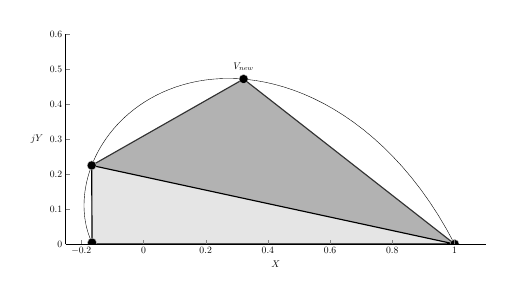
\begin{tikzpicture}[scale=0.35]

\begin{axis}[%
width=6in,
height=3in,
scale only axis,
axis on top=true,
xmin=-0.25,
xmax=1.1,
ymin=0,
ymax=0.6,
axis x line*=bottom,
axis y line*=left,
xlabel={$X$},
ylabel={$jY$},
xtick={-0.2,0,0.2,0.4,0.6,0.8,1},
ylabel style={rotate=-90},
ytick distance = 0.1
]
\addplot [color=black, forget plot]
  table[row sep=crcr]{%
1	0\\
0.97439570184454	0.0422189617067992\\
0.947664543045514	0.0822759496468887\\
0.919926652366486	0.120178744754836\\
0.891298754255365	0.155940000451509\\
0.8618940502982	0.189576974160811\\
0.831822115043362	0.221111260695846\\
0.801188805749226	0.250568528073344\\
0.770096185596349	0.277978256282022\\
0.738642459894664	0.303373479497687\\
0.706921924807467	0.326790532205477\\
0.675024928106738	0.34826879965765\\
0.643037841468705	0.367850473063845\\
0.611043043814387	0.385580309879881\\
0.579118915197029	0.401505399530848\\
0.547339840736992	0.415674934874619\\
0.515776224104452	0.428139989683019\\
0.484494510051408	0.438953302389642\\
0.453557215496707	0.448169066325949\\
0.423022968671182	0.455842726640583\\
0.392946555834355	0.462030784071105\\
0.363378975079551	0.466790605712337\\
0.334367496750526	0.47018024290145\\
0.305955729999881	0.472258256316704\\
0.278183695027438	0.473083548364434\\
0.251087900545453	0.472715202907487\\
0.224701426026886	0.471212332367794\\
0.199054008302929	0.468633932216212\\
0.174172132086558	0.465038742844109\\
0.150079124009928	0.460485118793442\\
0.126795249774977	0.455030905305267\\
0.104337814028549	0.448733322130736\\
0.0827212625856707	0.441648854533653\\
0.0619572866372231	0.433833151399599\\
0.0420549285911807	0.425340930353435\\
0.0230206892096995	0.416225889774718\\
0.00485863571765297	0.406540627589113\\
-0.0124294894283334	0.396336566703324\\
-0.0288441594077422	0.385663886941331\\
-0.0443879538246941	0.374571463330791\\
-0.0590654496872783	0.363106810580375\\
-0.0728831128341696	0.351316033581455\\
-0.0858491900514256	0.339243783761024\\
-0.0979736021088205	0.326933221106879\\
-0.109267837931654	0.314425981681024\\
-0.119744850110663	0.301762150432819\\
-0.129418951939533	0.288980239119696\\
-0.138305716156523	0.27611716914017\\
-0.146421875553965	0.263208259081419\\
-0.153785225606871	0.250287216781869\\
-0.160414529259544	0.237386135707918\\
-0.166329423997092	0.224535495443257\\
-0.171550331316981	0.211764166088996\\
-0.176098368704256	0.199099416373151\\
-0.179995264202967	0.1865669252688\\
-0.183263273665422	0.17419079692148\\
-0.185925100750451	0.161993578688022\\
-0.18800381973163	0.149996282091108\\
-0.189522801166623	0.138218406496255\\
-0.190505640469335	0.126677965320733\\
-0.190976089417432	0.11539151458703\\
-0.190957990619064	0.104374183636905\\
-0.190475214954231	0.0936397078257794\\
-0.18955160199825	0.083200463021171\\
-0.18821090342712	0.073067501733078\\
-0.186476729397344	0.0632505907086381\\
-0.18437249788586	0.0537582498279896\\
-0.181921386969236	0.0445977921430479\\
-0.179146290015116	0.0357753649058401\\
-0.176069773753131	0.0272959914381072\\
-0.172714039187066	0.0191636136990689\\
-0.169100885305011	0.0113811354135165\\
-0.16 0\\
};

\draw [color=Black!80, fill=Black!30, very thick] (-0.16, 0.00) -- (-0.166329423997092, 0.224535495443257) -- (0.3218, 0.4713) -- (1,0) -- (-0.165251675539513, 0.00395046562776303);

\draw [color=Black, fill=Gray!20, very thick] (-0.165251675539513, 0.00395046562776303) -- (-0.166329423997092, 0.224535495443257) -- (1,0) -- (-0.16, 0);

\node [circle, draw, Black!20, fill=Black!80, fill=Black, minimum size=1pt] at (-0.165251675539513, 0.00395046562776303) {};
\node [circle, draw, Black!20, fill=Black!80, fill=Black, minimum size=1pt] at (-0.166329423997092, 0.224535495443257) {};
\node [circle, draw, Black!20, fill=Black!80, fill=Black, minimum size=1pt] at (1,0) {};
\node [circle, draw, Black!20, fill=Black!80, fill=Black, minimum size=1pt, label=above:$V_{new}$] at (0.3218, 0.4713) {};

\end{axis}
\end{tikzpicture}%
      \caption{}
      \label{subfig:AproximacaoPoligonalZeta2}
  \end{subfigure}
  \\
  \begin{subfigure}[t]{0.4\columnwidth}
    % This file was created by matlab2tikz.
%
%The latest updates can be retrieved from
%  http://www.mathworks.com/matlabcentral/fileexchange/22022-matlab2tikz-matlab2tikz
%where you can also make suggestions and rate matlab2tikz.
%
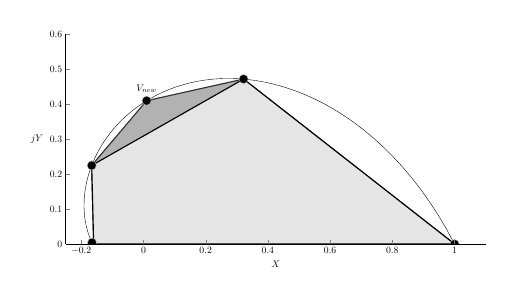
\begin{tikzpicture}[scale=0.35]

\begin{axis}[%
width=6in,
height=3in,
scale only axis,
axis on top=true,
xmin=-0.25,
xmax=1.1,
ymin=0,
ymax=0.6,
axis x line*=bottom,
axis y line*=left,
xlabel={$X$},
ylabel={$jY$},
xtick={-0.2,0,0.2,0.4,0.6,0.8,1},
ylabel style={rotate=-90},
ytick distance = 0.1
]
\addplot [color=black, forget plot]
  table[row sep=crcr]{%
1	0\\
0.97439570184454	0.0422189617067992\\
0.947664543045514	0.0822759496468887\\
0.919926652366486	0.120178744754836\\
0.891298754255365	0.155940000451509\\
0.8618940502982	0.189576974160811\\
0.831822115043362	0.221111260695846\\
0.801188805749226	0.250568528073344\\
0.770096185596349	0.277978256282022\\
0.738642459894664	0.303373479497687\\
0.706921924807467	0.326790532205477\\
0.675024928106738	0.34826879965765\\
0.643037841468705	0.367850473063845\\
0.611043043814387	0.385580309879881\\
0.579118915197029	0.401505399530848\\
0.547339840736992	0.415674934874619\\
0.515776224104452	0.428139989683019\\
0.484494510051408	0.438953302389642\\
0.453557215496707	0.448169066325949\\
0.423022968671182	0.455842726640583\\
0.392946555834355	0.462030784071105\\
0.363378975079551	0.466790605712337\\
0.334367496750526	0.47018024290145\\
0.305955729999881	0.472258256316704\\
0.278183695027438	0.473083548364434\\
0.251087900545453	0.472715202907487\\
0.224701426026886	0.471212332367794\\
0.199054008302929	0.468633932216212\\
0.174172132086558	0.465038742844109\\
0.150079124009928	0.460485118793442\\
0.126795249774977	0.455030905305267\\
0.104337814028549	0.448733322130736\\
0.0827212625856707	0.441648854533653\\
0.0619572866372231	0.433833151399599\\
0.0420549285911807	0.425340930353435\\
0.0230206892096995	0.416225889774718\\
0.00485863571765297	0.406540627589113\\
-0.0124294894283334	0.396336566703324\\
-0.0288441594077422	0.385663886941331\\
-0.0443879538246941	0.374571463330791\\
-0.0590654496872783	0.363106810580375\\
-0.0728831128341696	0.351316033581455\\
-0.0858491900514256	0.339243783761024\\
-0.0979736021088205	0.326933221106879\\
-0.109267837931654	0.314425981681024\\
-0.119744850110663	0.301762150432819\\
-0.129418951939533	0.288980239119696\\
-0.138305716156523	0.27611716914017\\
-0.146421875553965	0.263208259081419\\
-0.153785225606871	0.250287216781869\\
-0.160414529259544	0.237386135707918\\
-0.166329423997092	0.224535495443257\\
-0.171550331316981	0.211764166088996\\
-0.176098368704256	0.199099416373151\\
-0.179995264202967	0.1865669252688\\
-0.183263273665422	0.17419079692148\\
-0.185925100750451	0.161993578688022\\
-0.18800381973163	0.149996282091108\\
-0.189522801166623	0.138218406496255\\
-0.190505640469335	0.126677965320733\\
-0.190976089417432	0.11539151458703\\
-0.190957990619064	0.104374183636905\\
-0.190475214954231	0.0936397078257794\\
-0.18955160199825	0.083200463021171\\
-0.18821090342712	0.073067501733078\\
-0.186476729397344	0.0632505907086381\\
-0.18437249788586	0.0537582498279896\\
-0.181921386969236	0.0445977921430479\\
-0.179146290015116	0.0357753649058401\\
-0.176069773753131	0.0272959914381072\\
-0.172714039187066	0.0191636136990689\\
-0.169100885305011	0.0113811354135165\\
-0.16	0.0\\
};

\draw [color=Black!80, fill=Black!30, very thick] (-0.16, 0) -- (-0.166329423997092, 0.224535495443257) -- (0.0102, 0.4095) --(0.3218, 0.4713) -- (1,0) -- (-0.16, 0);

\draw [color=Black, fill=Gray!20, very thick] (-0.16, 0) -- (-0.166329423997092, 0.224535495443257) -- (0.3218, 0.4713) -- (1,0) -- (-0.16, 0);

\node [circle, draw, Black!20, fill=Black!80, fill=Black, minimum size=1pt] at (-0.165251675539513, 0.00395046562776303) {};
\node [circle, draw, Black!20, fill=Black!80, fill=Black, minimum size=1pt] at (-0.166329423997092, 0.224535495443257) {};
\node [circle, draw, Black!20, fill=Black!80, fill=Black, minimum size=1pt] at (1,0) {};
\node [circle, draw, Black!20, fill=Black!80, fill=Black, minimum size=1pt] at (0.3218, 0.4713) {};
\node [circle, draw, Black!20, fill=Black!80, fill=Black, minimum size=1pt, label=above:$V_{new}$] at (0.0102, 0.4095) {};
\end{axis}
\end{tikzpicture}%
    \caption{}
    \label{subfig:AproximacaoPoligonalZeta3}
  \end{subfigure}
  \begin{subfigure}[t]{0.4\columnwidth}
    % This file was created by matlab2tikz.
%
%The latest updates can be retrieved from
%  http://www.mathworks.com/matlabcentral/fileexchange/22022-matlab2tikz-matlab2tikz
%where you can also make suggestions and rate matlab2tikz.
%
\begin{tikzpicture}[scale=0.4]

\begin{axis}[%
width=6in,
height=3in,
scale only axis,
axis on top=true,
xmin=-0.25,
xmax=1.1,
ymin=0,
ymax=0.6,
axis x line*=bottom,
axis y line*=left,
xlabel={$X$},
ylabel={$jY$},
xtick={-0.2,0,0.2,0.4,0.6,0.8,1},
ylabel style={rotate=-90},
ytick distance = 0.1
]
\addplot [color=black, forget plot]
  table[row sep=crcr]{%
1	0\\
0.97439570184454	0.0422189617067992\\
0.947664543045514	0.0822759496468887\\
0.919926652366486	0.120178744754836\\
0.891298754255365	0.155940000451509\\
0.8618940502982	0.189576974160811\\
0.831822115043362	0.221111260695846\\
0.801188805749226	0.250568528073344\\
0.770096185596349	0.277978256282022\\
0.738642459894664	0.303373479497687\\
0.706921924807467	0.326790532205477\\
0.675024928106738	0.34826879965765\\
0.643037841468705	0.367850473063845\\
0.611043043814387	0.385580309879881\\
0.579118915197029	0.401505399530848\\
0.547339840736992	0.415674934874619\\
0.515776224104452	0.428139989683019\\
0.484494510051408	0.438953302389642\\
0.453557215496707	0.448169066325949\\
0.423022968671182	0.455842726640583\\
0.392946555834355	0.462030784071105\\
0.363378975079551	0.466790605712337\\
0.334367496750526	0.47018024290145\\
0.305955729999881	0.472258256316704\\
0.278183695027438	0.473083548364434\\
0.251087900545453	0.472715202907487\\
0.224701426026886	0.471212332367794\\
0.199054008302929	0.468633932216212\\
0.174172132086558	0.465038742844109\\
0.150079124009928	0.460485118793442\\
0.126795249774977	0.455030905305267\\
0.104337814028549	0.448733322130736\\
0.0827212625856707	0.441648854533653\\
0.0619572866372231	0.433833151399599\\
0.0420549285911807	0.425340930353435\\
0.0230206892096995	0.416225889774718\\
0.00485863571765297	0.406540627589113\\
-0.0124294894283334	0.396336566703324\\
-0.0288441594077422	0.385663886941331\\
-0.0443879538246941	0.374571463330791\\
-0.0590654496872783	0.363106810580375\\
-0.0728831128341696	0.351316033581455\\
-0.0858491900514256	0.339243783761024\\
-0.0979736021088205	0.326933221106879\\
-0.109267837931654	0.314425981681024\\
-0.119744850110663	0.301762150432819\\
-0.129418951939533	0.288980239119696\\
-0.138305716156523	0.27611716914017\\
-0.146421875553965	0.263208259081419\\
-0.153785225606871	0.250287216781869\\
-0.160414529259544	0.237386135707918\\
-0.166329423997092	0.224535495443257\\
-0.171550331316981	0.211764166088996\\
-0.176098368704256	0.199099416373151\\
-0.179995264202967	0.1865669252688\\
-0.183263273665422	0.17419079692148\\
-0.185925100750451	0.161993578688022\\
-0.18800381973163	0.149996282091108\\
-0.189522801166623	0.138218406496255\\
-0.190505640469335	0.126677965320733\\
-0.190976089417432	0.11539151458703\\
-0.190957990619064	0.104374183636905\\
-0.190475214954231	0.0936397078257794\\
-0.18955160199825	0.083200463021171\\
-0.18821090342712	0.073067501733078\\
-0.186476729397344	0.0632505907086381\\
-0.18437249788586	0.0537582498279896\\
-0.181921386969236	0.0445977921430479\\
-0.179146290015116	0.0357753649058401\\
-0.176069773753131	0.0272959914381072\\
-0.172714039187066	0.0191636136990689\\
-0.169100885305011	0.0113811354135165\\
-0.16	0\\
};

%\draw [color=Black!80, fill=Black!30, very thick] (-0.16, 0) -- (-0.166329423997092, 0.224535495443257) -- (0.3218, 0.4713) -- (0.6404, 0.3694) -- (1,0) -- (-0.16, 0);

%\draw [color=Black, fill=Gray!20, very thick] (-0.165251675539513, 0.00395046562776303) -- (-0.166329423997092, 0.224535495443257) -- (0.0102, 0.4095) -- (0.3218, 0.4713) -- (1,0) -- (-0.16, 0);

\draw [color=black!70, fill=Gray!40, very thick] (-0.16, 0) -- (-0.166329423997092, 0.224535495443257) -- (0.3218, 0.4713) -- (0.6404, 0.3694) -- (1,0) -- (-0.16, 0);

\draw [color=blue, fill=matlabb!70, very thick] (-0.165251675539513, 0.00395046562776303) -- (-0.166329423997092, 0.224535495443257) -- (0.0102, 0.4095) -- (0.3218, 0.4713) -- (1,0) -- (-0.16, 0);

\node [circle, draw, Black!20, fill=Black!80, fill=Black, minimum size=1pt] at (-0.165251675539513, 0.00395046562776303) {};
\node [circle, draw, Black!20, fill=Black!80, fill=Black, minimum size=1pt] at (-0.166329423997092, 0.224535495443257) {};
\node [circle, draw, Black!20, fill=Black!80, fill=Black, minimum size=1pt] at (1,0) {};
\node [circle, draw, Black!20, fill=Black!80, fill=Black, minimum size=1pt] at (0.3218, 0.4713) {};
\node [circle, draw, Black!20, fill=Black!80, fill=Black, minimum size=1pt] at (0.0102, 0.4095) {};
\node [circle, draw, Black!20, fill=Black!80, fill=Black, minimum size=1pt, label=above:$V_{new}$] at (0.6404, 0.3694) {};

\end{axis}
\end{tikzpicture}%
    \caption{}
    \label{subfig:AproximacaoPoligonalZeta4}
  \end{subfigure}
  \caption{As primeiras quatro aproximações poligonais da curva $\zeta$-constante.}
  \label{fig:AproximacoesPoligonalZeta}
\end{figure}

Para tal, utiliza-se o cálculo numérico para encontrar uma solução aproximada. Com tal ponto calculado e a não convexidade da cúspide tratada, é possível utilizar o algoritmo \ref{alg:AproximacaoPoligonalZeta}. Os vértices iniciais $V_o$ e $V_i$ do ramo são guardados em um vetor de vértices. Em paralelo a isso, os valores de $\omega_n$ que geram tais pontos também são armazenados. A cada iteração, o algoritmo calcula o ponto médio entre dois vértices consecutivos em cada vetor, já que a realização do primeiro depende do segundo.

\begin{algorithm}[!ht]
  \caption{Aproximação poligonal da região $\omega_n$-constante}\label{alg:AproximacaoPoligonalWn}
  \begin{algorithmic}[1]
    \Require $\sigma$, $\omega_n$, $T_s$
    \Ensure $K$
    \State $l \gets 0$
    \State $N_o \gets \z(\zeta_{min},\omega_n,T_s)$
    \State $N_i \gets \z(\zeta_{max},\omega_n,T_s)$
    \State $pontos3 \gets$ [$0$ $1$]
    \State $pontos4 \gets pontos3$
    \State $vec3 \gets$ [$N_i$ $N_o$]
    \State $vec4 \gets vec3$
    \State $F \gets P \succ 0$
    \State $F \gets \eqref{eq:LMIEstabilidadeRelativa}$ com $r = \exp{\left(-|\sigma|T_s\right)}$ \Comment{Taxa de amortecimento}
    \State $F \gets F \cap \eqref{eq:LMIESetorConicoDireito}$, com $\alpha = N_i$ e $\theta = \angulo(N_o,N_i)$ \Comment{Voltado para a direita}
    \State $F \gets F \cap \eqref{eq:LMIRightBounded}$, com $\alpha = N_i$ \Comment{Reta vertical}
    \State Verificar se o problema é factível
    \While{Problema for infactível}
      \If{$l < $ número de elementos em $vec3 - 1$}
        \State $l \gets l + 1$
      \Else
        \State $l \gets 1$
        \State $vec3 \gets vec4$
        \State $pontos1 \gets pontos2$
      \EndIf
        \State $F \gets$ \O \Comment{Descarta as restrições anteriores}
        \State $F \gets P \succ 0$
        \State $F \gets \eqref{eq:LMIEstabilidadeRelativa}$ com $r = \exp{\left(-|\sigma|T_s\right)}$ \Comment{Taxa de amortecimento}
        \State $ponto_{new} \gets (pontos3(l)+pontos3(l+1))/2$
        \State $V_{new2} \gets \z(ponto_{new2}, \omega_n, T_s)$
        \State $pontos4 \gets$ [$pontos4$ $ponto_{new2}$]
        \State Orderna de forma decrescente $pontos4$
        \State $vec4 \gets$ [$vec4$ $V_{new2}$]
        \State Orderna de forma decrescente $vec4$
        \State $F \gets F \cap \eqref{eq:LMIRightBounded}$, com $\alpha = V_i$ \Comment{Reta vertical}
        \For{$m = 1$ até número de elementos de $vec3-1$}
          \State $u_2 \gets \loc(vec4(m),vec4(m+1))$
          \State $F \gets F \cap \eqref{eq:LMIESetorConicoDireito}$, com $\alpha = u_2$ e $\theta = ang(vec4(m),u_2)$
        \EndFor
        \State Verificar se o problema é factível
    \EndWhile
    \State $K \gets ZP^{-1}$
  \end{algorithmic}
\end{algorithm}

Contudo, antes do algoritmo voltar para o início dos vetores, é preciso percorrer todos os pontos do vetor da iteração anterior\footnote{Como os vetores são atualizados com os novos elementos, o tamanho daqueles aumenta ($(n-1)$ pontos são adicionados a cada varredura, com $n$ a quantidade de pontos do vetor) durante a iteração. Assim, o execução termina antes de atingir o final do vetor.}. Para isso, cópias dos vetores de vértices e de pontos são inicializados, a fim de controlarem tal fluxo. Assim, quando o algoritmo terminar de percorrer o ``vetor anterior", tal conjunto é atualizado com os novos pontos e vértices calculados ao final deste processo.

Em relação ao cálculo dos pontos intermediários, a inclinação da reta que passa pelos pontos extremos locais pode ser positiva ou negativa. O uso da função $\loc$ se torna enssencial, pois caso o ponto resultante for menor que zero, a reta que passa pelos pontos possui inclinação positiva, e negativa caso contrário \cite{WISNIEWSKI2019}. Assim, os setores cônicos gerados seguem a orientação desta, com centro naquele ponto calculado.

A figura \ref{fig:AproximacoesPoligonalZeta} mostra as quatro primeira iterações do algoritmo \ref{alg:AproximacaoPoligonalZeta}. É possível observar o sentido horário do fluxo para o cálculo dos vértices intermediários. Também é notória a rápida abrangência da região $\zeta$-constante.

\begin{figure}[!hb]
  \centering
  \begin{subfigure}[t]{0.4\columnwidth}
      % This file was created by matlab2tikz.
%
%The latest updates can be retrieved from
%  http://www.mathworks.com/matlabcentral/fileexchange/22022-matlab2tikz-matlab2tikz
%where you can also make suggestions and rate matlab2tikz.
%
\begin{tikzpicture}

\begin{axis}[%
	font=\tiny,
	width=0.60037523452\textheight,
	height=0.8\textheight,
  scale only axis,
  axis on top=true,
  xmin=0.3,
  xmax=1.1,
  ymin=0,
  ymax=0.9,
  axis x line*=bottom,
  axis y line*=left,
  xlabel={$X$},
  ylabel={$jY$},
  xtick={0.4,0.5,0.6,0.7,0.8,0.9,1,1.1},
  xtick style={draw=black},
  ytick style={draw=black},
  ylabel style={rotate=-90},
  ytick distance = 0.1
  ]
  \addplot [color=black, forget plot]
    table[row sep=crcr]{%
  0.54030230586814	0.841470984807897\\
  0.534967863382191	0.833071460593297\\
  0.529768571049302	0.82470279512119\\
  0.524701459880193	0.816365672712812\\
  0.519763623176388	0.808060717031331\\
  0.514952215250233	0.799788493318601\\
  0.510264450170919	0.791549510522827\\
  0.505697600535993	0.78334422332136\\
  0.501248996267831	0.775173034042531\\
  0.49691602343458	0.767036294490186\\
  0.492696123095076	0.758934307674296\\
  0.488586790167236	0.750867329450786\\
  0.484585572319477	0.742835570073457\\
  0.480690068884672	0.734839195660667\\
  0.476897929796208	0.726878329579179\\
  0.473206854545681	0.718953053747392\\
  0.46961459116181	0.71106340985992\\
  0.466118935210123	0.703209400535282\\
  0.462717728813013	0.695390990388255\\
  0.459408859689731	0.687608107028223\\
  0.456190260215944	0.679860641984627\\
  0.453059906502422	0.672148451560422\\
  0.450015817492511	0.664471357614223\\
  0.447056054077976	0.65682914827157\\
  0.444178718232864	0.649221578565555\\
  0.441381952165015	0.641648371006764\\
  0.438663937484865	0.634109216082268\\
  0.436022894391196	0.626603772683115\\
  0.433457080873477	0.619131668459512\\
  0.430964791930477	0.611692500102562\\
  0.428544358804814	0.604285833551141\\
  0.42619414823311	0.596911204122128\\
  0.42391256171145	0.589568116561847\\
  0.421698034775829	0.582256045016197\\
  0.419549036297272	0.574974432916473\\
  0.41746406779136	0.567722692777469\\
  0.415441662741833	0.560500205903863\\
  0.413480385938019	0.553306322000374\\
  0.411578832825784	0.546140358680509\\
  0.409735628871742	0.539001600868033\\
  0.407949428940455	0.531889300084499\\
  0.40621891668436	0.524802673615316\\
  0.404542803946157	0.517740903545838\\
  0.40291983017342	0.510703135657861\\
  0.401348761845173	0.503688478175676\\
  0.399828391910187	0.496696000349422\\
  0.398357539236775	0.489724730861874\\
  0.396935048073831	0.482773656043023\\
  0.395559787522899	0.475841717874705\\
  0.394230651021055	0.468927811765217\\
  0.392946555834355	0.462030784071105\\
  0.391706442561671	0.455149429340254\\
  0.390509274648673	0.448282487246767\\
  0.389354037911772	0.44142863918402\\
  0.388239740071813	0.434586504477429\\
  0.387165410297317	0.427754636172876\\
  0.386130098757092	0.420931516350199\\
  0.385132876182003	0.414115550903467\\
  0.384172833435737	0.407305063720748\\
  0.383249081094361	0.400498290185438\\
  0.382360749034503	0.393693369908582\\
  0.381506986029992	0.386888338586634\\
  0.380686959356758	0.380081118861167\\
  0.379899854405851	0.373269510035555\\
  0.379144874304403	0.366451176477703\\
  0.378421239544366	0.359623634506574\\
  0.377728187618882	0.352784237522037\\
  0.377064972666117	0.345930159090858\\
  0.376430865120411	0.339058373644207\\
  0.375825151370604	0.332165634370895\\
  0.37524713342538	0.325248447802048\\
  0.374696128585488	0.318303044471906\\
  0.374171469122712	0.311325344899309\\
  0.373672501965436	0.3043109199563\\
  0.373198588390686	0.297254944461841\\
  0.3727491037225	0.290152142543361\\
  0.372323437036515	0.28299672292366\\
  0.371920990870632	0.275782301783101\\
  0.37154118094164	0.268501810171284\\
  0.371183435867678	0.261147382032347\\
  0.370847196896416	0.253710217667177\\
  0.370531917638833	0.246180415741187\\
  0.370237063808491	0.238546764541796\\
  0.36996211296618	0.230796479763275\\
  0.369706554269828	0.222914871126492\\
  0.369469888229576	0.214884912789054\\
  0.369251626467901	0.206686681385867\\
  0.369051291484697	0.19829660831813\\
  0.368868416427202	0.189686465478007\\
  0.368702544864672	0.180821958508667\\
  0.368553230567724	0.171660724860641\\
  0.368420037292221	0.162149397333074\\
  0.368302538567639	0.152219138716371\\
  0.368200317489797	0.141778547631191\\
  0.368112966517885	0.130701758359581\\
  0.368040087275681	0.118807042639501\\
  0.367981290356887	0.105814611834237\\
  0.367936195134494	0.0912518826526587\\
  0.367904429574089	0.0741940133758049\\
  0.367885630051037	0.0522436648106183\\
  0.367879441171442	0\\
  };
  \addplot [color=black!70, fill=Gray!40, very thick]
    table[row sep=crcr]{%
  1	0\\
  0.999950000416665	0.00999983333416666\\
  0.999800006666578	0.0199986666933331\\
  0.999550033748988	0.0299955002024957\\
  0.999200106660978	0.0399893341866342\\
  0.998750260394966	0.0499791692706783\\
  0.998200539935204	0.0599640064794446\\
  0.99755100025328	0.0699428473375328\\
  0.996801706302619	0.0799146939691727\\
  0.995952733011994	0.089878549198011\\
  0.995004165278026	0.0998334166468282\\
  0.993956097956697	0.109778300837175\\
  0.992808635853866	0.119712207288919\\
  0.991561893714788	0.129634142619695\\
  0.990215996212637	0.139543114644236\\
  0.988771077936042	0.149438132473599\\
  0.987227283375627	0.159318206614246\\
  0.985584766909561	0.169182349066996\\
  0.983843692788121	0.179029573425824\\
  0.98200423511727	0.188858894976501\\
  0.980066577841242	0.198669330795061\\
  0.978030914724148	0.2084598998461\\
  0.975897449330606	0.218229623080869\\
  0.973666395005375	0.227977523535188\\
  0.97133797485203	0.237702626427135\\
  0.968912421710645	0.247403959254523\\
  0.966389978134513	0.257080551892155\\
  0.963770896365891	0.266731436688831\\
  0.961055438310771	0.276355648564114\\
  0.958243875512697	0.285952225104836\\
  0.955336489125606	0.29552020666134\\
  0.952333569885713	0.305058636443443\\
  0.949235418082441	0.314566560616118\\
  0.946042343528387	0.324043028394868\\
  0.942754665528346	0.333487092140814\\
  0.939372712847379	0.342897807455451\\
  0.935896823677935	0.35227423327509\\
  0.932327345606034	0.361615431964962\\
  0.92866463557651	0.370920469412983\\
  0.924909059857313	0.380188415123161\\
  0.921060994002885	0.389418342308651\\
  0.917120822816605	0.398609327984423\\
  0.913088940312308	0.40776045305957\\
  0.908965749674885	0.416870802429211\\
  0.904751663219963	0.425939465066\\
  0.900447102352677	0.43496553411123\\
  0.896052497525525	0.44394810696552\\
  0.891568288195329	0.452886285379068\\
  0.886994922779284	0.461779175541483\\
  0.882332858610121	0.470625888171158\\
  0.877582561890373	0.479425538604203\\
  0.872744507645751	0.488177246882908\\
  0.86781917967765	0.496880137843737\\
  0.862807070514761	0.505533341204847\\
  0.857708681363824	0.514135991653113\\
  0.852524522059506	0.522687228930659\\
  0.847255111013416	0.531186197920883\\
  0.841900975162269	0.539632048733969\\
  0.836462649915187	0.548023936791874\\
  0.830940679100164	0.556361022912784\\
  0.825335614909678	0.564642473395035\\
  0.819648017845479	0.572867460100481\\
  0.813878456662534	0.581035160537305\\
  0.808027508312152	0.58914475794227\\
  0.802095757884293	0.597195441362392\\
  0.796083798549056	0.605186405736039\\
  0.789992231497365	0.613116851973434\\
  0.783821665880849	0.62098598703656\\
  0.777572718750928	0.628793024018468\\
  0.771246014997107	0.636537182221968\\
  0.764842187284488	0.644217687237691\\
  0.758361875990508	0.651833771021537\\
  0.751805729140895	0.659384671971473\\
  0.74517440234487	0.666869635003698\\
  0.738468558729588	0.674287911628145\\
  0.731688868873821	0.681638760023334\\
  0.724836010740905	0.688921445110551\\
  0.717910669610943	0.696135238627357\\
  0.710913538012277	0.70327941920041\\
  0.703845315652236	0.710353272417608\\
  0.696706709347165	0.717356090899523\\
  0.689498432951747	0.724287174370143\\
  0.682221207287613	0.731145829726896\\
  0.674875760071267	0.737931371109963\\
  0.667462825841308	0.744643119970859\\
  0.659983145884982	0.751280405140293\\
  0.652437468164052	0.757842562895277\\
  0.644826547240001	0.764328937025505\\
  0.63715114419858	0.770738878898969\\
  0.629412026573697	0.777071747526824\\
  0.621609968270664	0.783326909627483\\
  0.613745749488812	0.78950373968995\\
  0.605820156643463	0.795601620036366\\
  0.597833982287298	0.801619940883777\\
  0.589788025031098	0.807558100405114\\
  0.581683089463883	0.813415504789374\\
  0.573519986072457	0.819191568300998\\
  0.565299531160354	0.82488571333845\\
  0.557022546766217	0.83049737049197\\
  0.548689860581588	0.836025978600521\\
  0.54030230586814	0.841470984807897\\
  0.367879441171442 0\\
  1 0\\
  };
  
  \node [circle, draw, Magenta, fill=black, minimum size=1pt, label=above right:$R$, scale=0.5] at (0.367879441171442, 0) {};
  \node [circle, draw, Magenta, fill=black, minimum size=1pt, label=left:$Q$, scale=0.5] at (0.54030230586814, 0.841470984807897) {};
  
  \end{axis}
  \end{tikzpicture}%
      \caption{}
      \label{subfig:AproximacaoPoligonalWn1}
  \end{subfigure}
  \begin{subfigure}[t]{0.4\columnwidth}
      % This file was created by matlab2tikz.
%
%The latest updates can be retrieved from
%  http://www.mathworks.com/matlabcentral/fileexchange/22022-matlab2tikz-matlab2tikz
%where you can also make suggestions and rate matlab2tikz.
%
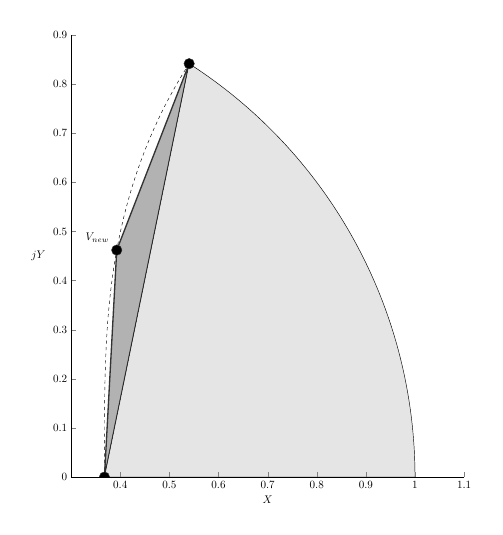
\begin{tikzpicture}[scale=0.4]

  \begin{axis}[%
  width=4.913in,
  height=5.527in,
  scale only axis,
  axis on top=true,
  xmin=0.3,
  xmax=1.1,
  ymin=0,
  ymax=0.9,
  axis x line*=bottom,
  axis y line*=left,
  xlabel={$X$},
  ylabel={$jY$},
  xtick={0.4,0.5,0.6,0.7,0.8,0.9,1,1.1},
  ylabel style={rotate=-90},
  ytick distance = 0.1
  ]
  \addplot [color=black, dashed, forget plot]
    table[row sep=crcr]{%
  0.54030230586814	0.841470984807897\\
  0.534967863382191	0.833071460593297\\
  0.529768571049302	0.82470279512119\\
  0.524701459880193	0.816365672712812\\
  0.519763623176388	0.808060717031331\\
  0.514952215250233	0.799788493318601\\
  0.510264450170919	0.791549510522827\\
  0.505697600535993	0.78334422332136\\
  0.501248996267831	0.775173034042531\\
  0.49691602343458	0.767036294490186\\
  0.492696123095076	0.758934307674296\\
  0.488586790167236	0.750867329450786\\
  0.484585572319477	0.742835570073457\\
  0.480690068884672	0.734839195660667\\
  0.476897929796208	0.726878329579179\\
  0.473206854545681	0.718953053747392\\
  0.46961459116181	0.71106340985992\\
  0.466118935210123	0.703209400535282\\
  0.462717728813013	0.695390990388255\\
  0.459408859689731	0.687608107028223\\
  0.456190260215944	0.679860641984627\\
  0.453059906502422	0.672148451560422\\
  0.450015817492511	0.664471357614223\\
  0.447056054077976	0.65682914827157\\
  0.444178718232864	0.649221578565555\\
  0.441381952165015	0.641648371006764\\
  0.438663937484865	0.634109216082268\\
  0.436022894391196	0.626603772683115\\
  0.433457080873477	0.619131668459512\\
  0.430964791930477	0.611692500102562\\
  0.428544358804814	0.604285833551141\\
  0.42619414823311	0.596911204122128\\
  0.42391256171145	0.589568116561847\\
  0.421698034775829	0.582256045016197\\
  0.419549036297272	0.574974432916473\\
  0.41746406779136	0.567722692777469\\
  0.415441662741833	0.560500205903863\\
  0.413480385938019	0.553306322000374\\
  0.411578832825784	0.546140358680509\\
  0.409735628871742	0.539001600868033\\
  0.407949428940455	0.531889300084499\\
  0.40621891668436	0.524802673615316\\
  0.404542803946157	0.517740903545838\\
  0.40291983017342	0.510703135657861\\
  0.401348761845173	0.503688478175676\\
  0.399828391910187	0.496696000349422\\
  0.398357539236775	0.489724730861874\\
  0.396935048073831	0.482773656043023\\
  0.395559787522899	0.475841717874705\\
  0.394230651021055	0.468927811765217\\
  0.392946555834355	0.462030784071105\\
  0.391706442561671	0.455149429340254\\
  0.390509274648673	0.448282487246767\\
  0.389354037911772	0.44142863918402\\
  0.388239740071813	0.434586504477429\\
  0.387165410297317	0.427754636172876\\
  0.386130098757092	0.420931516350199\\
  0.385132876182003	0.414115550903467\\
  0.384172833435737	0.407305063720748\\
  0.383249081094361	0.400498290185438\\
  0.382360749034503	0.393693369908582\\
  0.381506986029992	0.386888338586634\\
  0.380686959356758	0.380081118861167\\
  0.379899854405851	0.373269510035555\\
  0.379144874304403	0.366451176477703\\
  0.378421239544366	0.359623634506574\\
  0.377728187618882	0.352784237522037\\
  0.377064972666117	0.345930159090858\\
  0.376430865120411	0.339058373644207\\
  0.375825151370604	0.332165634370895\\
  0.37524713342538	0.325248447802048\\
  0.374696128585488	0.318303044471906\\
  0.374171469122712	0.311325344899309\\
  0.373672501965436	0.3043109199563\\
  0.373198588390686	0.297254944461841\\
  0.3727491037225	0.290152142543361\\
  0.372323437036515	0.28299672292366\\
  0.371920990870632	0.275782301783101\\
  0.37154118094164	0.268501810171284\\
  0.371183435867678	0.261147382032347\\
  0.370847196896416	0.253710217667177\\
  0.370531917638833	0.246180415741187\\
  0.370237063808491	0.238546764541796\\
  0.36996211296618	0.230796479763275\\
  0.369706554269828	0.222914871126492\\
  0.369469888229576	0.214884912789054\\
  0.369251626467901	0.206686681385867\\
  0.369051291484697	0.19829660831813\\
  0.368868416427202	0.189686465478007\\
  0.368702544864672	0.180821958508667\\
  0.368553230567724	0.171660724860641\\
  0.368420037292221	0.162149397333074\\
  0.368302538567639	0.152219138716371\\
  0.368200317489797	0.141778547631191\\
  0.368112966517885	0.130701758359581\\
  0.368040087275681	0.118807042639501\\
  0.367981290356887	0.105814611834237\\
  0.367936195134494	0.0912518826526587\\
  0.367904429574089	0.0741940133758049\\
  0.367885630051037	0.0522436648106183\\
  0.367879441171442	0\\
  };

  \draw [color=Black!80, fill=Black!30, very thick] (0.367879441171442, 0) -- (0.3929, 0.4620) -- (0.54030230586814, 0.841470984807897) -- (0.367879441171442, 0);

  \addplot [color=Black, fill=Gray!20, forget plot]
    table[row sep=crcr]{%
  1	0\\
  0.999950000416665	0.00999983333416666\\
  0.999800006666578	0.0199986666933331\\
  0.999550033748988	0.0299955002024957\\
  0.999200106660978	0.0399893341866342\\
  0.998750260394966	0.0499791692706783\\
  0.998200539935204	0.0599640064794446\\
  0.99755100025328	0.0699428473375328\\
  0.996801706302619	0.0799146939691727\\
  0.995952733011994	0.089878549198011\\
  0.995004165278026	0.0998334166468282\\
  0.993956097956697	0.109778300837175\\
  0.992808635853866	0.119712207288919\\
  0.991561893714788	0.129634142619695\\
  0.990215996212637	0.139543114644236\\
  0.988771077936042	0.149438132473599\\
  0.987227283375627	0.159318206614246\\
  0.985584766909561	0.169182349066996\\
  0.983843692788121	0.179029573425824\\
  0.98200423511727	0.188858894976501\\
  0.980066577841242	0.198669330795061\\
  0.978030914724148	0.2084598998461\\
  0.975897449330606	0.218229623080869\\
  0.973666395005375	0.227977523535188\\
  0.97133797485203	0.237702626427135\\
  0.968912421710645	0.247403959254523\\
  0.966389978134513	0.257080551892155\\
  0.963770896365891	0.266731436688831\\
  0.961055438310771	0.276355648564114\\
  0.958243875512697	0.285952225104836\\
  0.955336489125606	0.29552020666134\\
  0.952333569885713	0.305058636443443\\
  0.949235418082441	0.314566560616118\\
  0.946042343528387	0.324043028394868\\
  0.942754665528346	0.333487092140814\\
  0.939372712847379	0.342897807455451\\
  0.935896823677935	0.35227423327509\\
  0.932327345606034	0.361615431964962\\
  0.92866463557651	0.370920469412983\\
  0.924909059857313	0.380188415123161\\
  0.921060994002885	0.389418342308651\\
  0.917120822816605	0.398609327984423\\
  0.913088940312308	0.40776045305957\\
  0.908965749674885	0.416870802429211\\
  0.904751663219963	0.425939465066\\
  0.900447102352677	0.43496553411123\\
  0.896052497525525	0.44394810696552\\
  0.891568288195329	0.452886285379068\\
  0.886994922779284	0.461779175541483\\
  0.882332858610121	0.470625888171158\\
  0.877582561890373	0.479425538604203\\
  0.872744507645751	0.488177246882908\\
  0.86781917967765	0.496880137843737\\
  0.862807070514761	0.505533341204847\\
  0.857708681363824	0.514135991653113\\
  0.852524522059506	0.522687228930659\\
  0.847255111013416	0.531186197920883\\
  0.841900975162269	0.539632048733969\\
  0.836462649915187	0.548023936791874\\
  0.830940679100164	0.556361022912784\\
  0.825335614909678	0.564642473395035\\
  0.819648017845479	0.572867460100481\\
  0.813878456662534	0.581035160537305\\
  0.808027508312152	0.58914475794227\\
  0.802095757884293	0.597195441362392\\
  0.796083798549056	0.605186405736039\\
  0.789992231497365	0.613116851973434\\
  0.783821665880849	0.62098598703656\\
  0.777572718750928	0.628793024018468\\
  0.771246014997107	0.636537182221968\\
  0.764842187284488	0.644217687237691\\
  0.758361875990508	0.651833771021537\\
  0.751805729140895	0.659384671971473\\
  0.74517440234487	0.666869635003698\\
  0.738468558729588	0.674287911628145\\
  0.731688868873821	0.681638760023334\\
  0.724836010740905	0.688921445110551\\
  0.717910669610943	0.696135238627357\\
  0.710913538012277	0.70327941920041\\
  0.703845315652236	0.710353272417608\\
  0.696706709347165	0.717356090899523\\
  0.689498432951747	0.724287174370143\\
  0.682221207287613	0.731145829726896\\
  0.674875760071267	0.737931371109963\\
  0.667462825841308	0.744643119970859\\
  0.659983145884982	0.751280405140293\\
  0.652437468164052	0.757842562895277\\
  0.644826547240001	0.764328937025505\\
  0.63715114419858	0.770738878898969\\
  0.629412026573697	0.777071747526824\\
  0.621609968270664	0.783326909627483\\
  0.613745749488812	0.78950373968995\\
  0.605820156643463	0.795601620036366\\
  0.597833982287298	0.801619940883777\\
  0.589788025031098	0.807558100405114\\
  0.581683089463883	0.813415504789374\\
  0.573519986072457	0.819191568300998\\
  0.565299531160354	0.82488571333845\\
  0.557022546766217	0.83049737049197\\
  0.548689860581588	0.836025978600521\\
  0.54030230586814	0.841470984807897\\
  0.367879441171442 0\\
  1 0\\
  };

  \node [circle, draw, Black!80, fill=Black!80, fill=Black, minimum size=1pt] at (0.367879441171442, 0) {};
  \node [circle, draw, Black!80, fill=Black!80, fill=Black, minimum size=1pt] at (0.54030230586814, 0.841470984807897) {};
  \node [circle, draw, Black!80, fill=Black!80, fill=Black, minimum size=1pt, label=above left:$V_{new}$] at (0.3929, 0.4620) {};

  \end{axis}
  \end{tikzpicture}%
      \caption{}
      \label{subfig:AproximacaoPoligonalWn2}
  \end{subfigure}
  \\
  \begin{subfigure}[t]{0.4\columnwidth}
    % This file was created by matlab2tikz.
%
%The latest updates can be retrieved from
%  http://www.mathworks.com/matlabcentral/fileexchange/22022-matlab2tikz-matlab2tikz
%where you can also make suggestions and rate matlab2tikz.
%
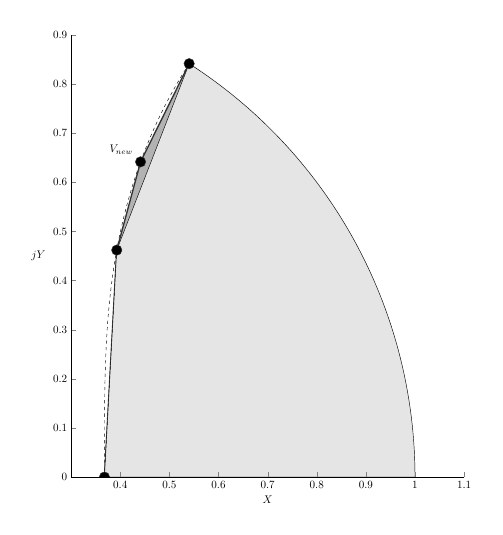
\begin{tikzpicture}[scale=0.4]

  \begin{axis}[%
  width=4.913in,
  height=5.527in,
  scale only axis,
  axis on top=true,
  xmin=0.3,
  xmax=1.1,
  ymin=0,
  ymax=0.9,
  axis x line*=bottom,
  axis y line*=left,
  xlabel={$X$},
  ylabel={$jY$},
  xtick={0.4,0.5,0.6,0.7,0.8,0.9,1,1.1},
  ylabel style={rotate=-90},
  ytick distance = 0.1
  ]
  \addplot [color=black, dashed, forget plot]
    table[row sep=crcr]{%
  0.54030230586814	0.841470984807897\\
  0.534967863382191	0.833071460593297\\
  0.529768571049302	0.82470279512119\\
  0.524701459880193	0.816365672712812\\
  0.519763623176388	0.808060717031331\\
  0.514952215250233	0.799788493318601\\
  0.510264450170919	0.791549510522827\\
  0.505697600535993	0.78334422332136\\
  0.501248996267831	0.775173034042531\\
  0.49691602343458	0.767036294490186\\
  0.492696123095076	0.758934307674296\\
  0.488586790167236	0.750867329450786\\
  0.484585572319477	0.742835570073457\\
  0.480690068884672	0.734839195660667\\
  0.476897929796208	0.726878329579179\\
  0.473206854545681	0.718953053747392\\
  0.46961459116181	0.71106340985992\\
  0.466118935210123	0.703209400535282\\
  0.462717728813013	0.695390990388255\\
  0.459408859689731	0.687608107028223\\
  0.456190260215944	0.679860641984627\\
  0.453059906502422	0.672148451560422\\
  0.450015817492511	0.664471357614223\\
  0.447056054077976	0.65682914827157\\
  0.444178718232864	0.649221578565555\\
  0.441381952165015	0.641648371006764\\
  0.438663937484865	0.634109216082268\\
  0.436022894391196	0.626603772683115\\
  0.433457080873477	0.619131668459512\\
  0.430964791930477	0.611692500102562\\
  0.428544358804814	0.604285833551141\\
  0.42619414823311	0.596911204122128\\
  0.42391256171145	0.589568116561847\\
  0.421698034775829	0.582256045016197\\
  0.419549036297272	0.574974432916473\\
  0.41746406779136	0.567722692777469\\
  0.415441662741833	0.560500205903863\\
  0.413480385938019	0.553306322000374\\
  0.411578832825784	0.546140358680509\\
  0.409735628871742	0.539001600868033\\
  0.407949428940455	0.531889300084499\\
  0.40621891668436	0.524802673615316\\
  0.404542803946157	0.517740903545838\\
  0.40291983017342	0.510703135657861\\
  0.401348761845173	0.503688478175676\\
  0.399828391910187	0.496696000349422\\
  0.398357539236775	0.489724730861874\\
  0.396935048073831	0.482773656043023\\
  0.395559787522899	0.475841717874705\\
  0.394230651021055	0.468927811765217\\
  0.392946555834355	0.462030784071105\\
  0.391706442561671	0.455149429340254\\
  0.390509274648673	0.448282487246767\\
  0.389354037911772	0.44142863918402\\
  0.388239740071813	0.434586504477429\\
  0.387165410297317	0.427754636172876\\
  0.386130098757092	0.420931516350199\\
  0.385132876182003	0.414115550903467\\
  0.384172833435737	0.407305063720748\\
  0.383249081094361	0.400498290185438\\
  0.382360749034503	0.393693369908582\\
  0.381506986029992	0.386888338586634\\
  0.380686959356758	0.380081118861167\\
  0.379899854405851	0.373269510035555\\
  0.379144874304403	0.366451176477703\\
  0.378421239544366	0.359623634506574\\
  0.377728187618882	0.352784237522037\\
  0.377064972666117	0.345930159090858\\
  0.376430865120411	0.339058373644207\\
  0.375825151370604	0.332165634370895\\
  0.37524713342538	0.325248447802048\\
  0.374696128585488	0.318303044471906\\
  0.374171469122712	0.311325344899309\\
  0.373672501965436	0.3043109199563\\
  0.373198588390686	0.297254944461841\\
  0.3727491037225	0.290152142543361\\
  0.372323437036515	0.28299672292366\\
  0.371920990870632	0.275782301783101\\
  0.37154118094164	0.268501810171284\\
  0.371183435867678	0.261147382032347\\
  0.370847196896416	0.253710217667177\\
  0.370531917638833	0.246180415741187\\
  0.370237063808491	0.238546764541796\\
  0.36996211296618	0.230796479763275\\
  0.369706554269828	0.222914871126492\\
  0.369469888229576	0.214884912789054\\
  0.369251626467901	0.206686681385867\\
  0.369051291484697	0.19829660831813\\
  0.368868416427202	0.189686465478007\\
  0.368702544864672	0.180821958508667\\
  0.368553230567724	0.171660724860641\\
  0.368420037292221	0.162149397333074\\
  0.368302538567639	0.152219138716371\\
  0.368200317489797	0.141778547631191\\
  0.368112966517885	0.130701758359581\\
  0.368040087275681	0.118807042639501\\
  0.367981290356887	0.105814611834237\\
  0.367936195134494	0.0912518826526587\\
  0.367904429574089	0.0741940133758049\\
  0.367885630051037	0.0522436648106183\\
  0.367879441171442	0\\
  };

  \draw [color=Black!80, fill=Black!30, very thick] (0.367879441171442, 0) -- (0.3929, 0.4620) -- (0.4414, 0.6416) -- (0.54030230586814, 0.841470984807897) -- (0.367879441171442, 0);

  \addplot [color=Black, fill=Gray!20, forget plot]
    table[row sep=crcr]{%
  1	0\\
  0.999950000416665	0.00999983333416666\\
  0.999800006666578	0.0199986666933331\\
  0.999550033748988	0.0299955002024957\\
  0.999200106660978	0.0399893341866342\\
  0.998750260394966	0.0499791692706783\\
  0.998200539935204	0.0599640064794446\\
  0.99755100025328	0.0699428473375328\\
  0.996801706302619	0.0799146939691727\\
  0.995952733011994	0.089878549198011\\
  0.995004165278026	0.0998334166468282\\
  0.993956097956697	0.109778300837175\\
  0.992808635853866	0.119712207288919\\
  0.991561893714788	0.129634142619695\\
  0.990215996212637	0.139543114644236\\
  0.988771077936042	0.149438132473599\\
  0.987227283375627	0.159318206614246\\
  0.985584766909561	0.169182349066996\\
  0.983843692788121	0.179029573425824\\
  0.98200423511727	0.188858894976501\\
  0.980066577841242	0.198669330795061\\
  0.978030914724148	0.2084598998461\\
  0.975897449330606	0.218229623080869\\
  0.973666395005375	0.227977523535188\\
  0.97133797485203	0.237702626427135\\
  0.968912421710645	0.247403959254523\\
  0.966389978134513	0.257080551892155\\
  0.963770896365891	0.266731436688831\\
  0.961055438310771	0.276355648564114\\
  0.958243875512697	0.285952225104836\\
  0.955336489125606	0.29552020666134\\
  0.952333569885713	0.305058636443443\\
  0.949235418082441	0.314566560616118\\
  0.946042343528387	0.324043028394868\\
  0.942754665528346	0.333487092140814\\
  0.939372712847379	0.342897807455451\\
  0.935896823677935	0.35227423327509\\
  0.932327345606034	0.361615431964962\\
  0.92866463557651	0.370920469412983\\
  0.924909059857313	0.380188415123161\\
  0.921060994002885	0.389418342308651\\
  0.917120822816605	0.398609327984423\\
  0.913088940312308	0.40776045305957\\
  0.908965749674885	0.416870802429211\\
  0.904751663219963	0.425939465066\\
  0.900447102352677	0.43496553411123\\
  0.896052497525525	0.44394810696552\\
  0.891568288195329	0.452886285379068\\
  0.886994922779284	0.461779175541483\\
  0.882332858610121	0.470625888171158\\
  0.877582561890373	0.479425538604203\\
  0.872744507645751	0.488177246882908\\
  0.86781917967765	0.496880137843737\\
  0.862807070514761	0.505533341204847\\
  0.857708681363824	0.514135991653113\\
  0.852524522059506	0.522687228930659\\
  0.847255111013416	0.531186197920883\\
  0.841900975162269	0.539632048733969\\
  0.836462649915187	0.548023936791874\\
  0.830940679100164	0.556361022912784\\
  0.825335614909678	0.564642473395035\\
  0.819648017845479	0.572867460100481\\
  0.813878456662534	0.581035160537305\\
  0.808027508312152	0.58914475794227\\
  0.802095757884293	0.597195441362392\\
  0.796083798549056	0.605186405736039\\
  0.789992231497365	0.613116851973434\\
  0.783821665880849	0.62098598703656\\
  0.777572718750928	0.628793024018468\\
  0.771246014997107	0.636537182221968\\
  0.764842187284488	0.644217687237691\\
  0.758361875990508	0.651833771021537\\
  0.751805729140895	0.659384671971473\\
  0.74517440234487	0.666869635003698\\
  0.738468558729588	0.674287911628145\\
  0.731688868873821	0.681638760023334\\
  0.724836010740905	0.688921445110551\\
  0.717910669610943	0.696135238627357\\
  0.710913538012277	0.70327941920041\\
  0.703845315652236	0.710353272417608\\
  0.696706709347165	0.717356090899523\\
  0.689498432951747	0.724287174370143\\
  0.682221207287613	0.731145829726896\\
  0.674875760071267	0.737931371109963\\
  0.667462825841308	0.744643119970859\\
  0.659983145884982	0.751280405140293\\
  0.652437468164052	0.757842562895277\\
  0.644826547240001	0.764328937025505\\
  0.63715114419858	0.770738878898969\\
  0.629412026573697	0.777071747526824\\
  0.621609968270664	0.783326909627483\\
  0.613745749488812	0.78950373968995\\
  0.605820156643463	0.795601620036366\\
  0.597833982287298	0.801619940883777\\
  0.589788025031098	0.807558100405114\\
  0.581683089463883	0.813415504789374\\
  0.573519986072457	0.819191568300998\\
  0.565299531160354	0.82488571333845\\
  0.557022546766217	0.83049737049197\\
  0.548689860581588	0.836025978600521\\
  0.54030230586814	0.841470984807897\\
  0.3929 0.4620\\
  0.367879441171442 0\\
  1 0\\
  };

  \node [circle, draw, Black!80, fill=Black!80, fill=Black, minimum size=1pt] at (0.367879441171442, 0) {};
  \node [circle, draw, Black!80, fill=Black!80, fill=Black, minimum size=1pt] at (0.54030230586814, 0.841470984807897) {};
  \node [circle, draw, Black!80, fill=Black!80, fill=Black, minimum size=1pt] at (0.3929, 0.4620) {};
  \node [circle, draw, Black!80, fill=Black!80, fill=Black, minimum size=1pt, label=above left:$V_{new}$] at (0.4414, 0.6416) {};

  \end{axis}
  \end{tikzpicture}%
    \caption{}
    \label{subfig:AproximacaoPoligonalWn3}
  \end{subfigure}
  \begin{subfigure}[t]{0.4\columnwidth}
    % This file was created by matlab2tikz.
%
%The latest updates can be retrieved from
%  http://www.mathworks.com/matlabcentral/fileexchange/22022-matlab2tikz-matlab2tikz
%where you can also make suggestions and rate matlab2tikz.
%
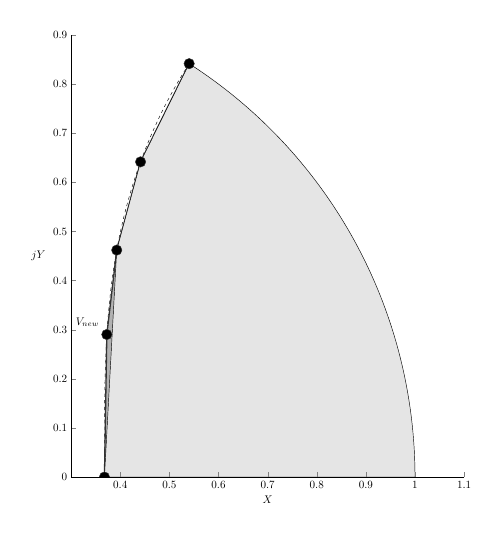
\begin{tikzpicture}[scale=0.4]

  \begin{axis}[%
  width=4.913in,
  height=5.527in,
  scale only axis,
  axis on top=true,
  xmin=0.3,
  xmax=1.1,
  ymin=0,
  ymax=0.9,
  axis x line*=bottom,
  axis y line*=left,
  xlabel={$X$},
  ylabel={$jY$},
  xtick={0.4,0.5,0.6,0.7,0.8,0.9,1,1.1},
  ylabel style={rotate=-90},
  ytick distance = 0.1
  ]
  \addplot [color=black, dashed, forget plot]
    table[row sep=crcr]{%
  0.54030230586814	0.841470984807897\\
  0.534967863382191	0.833071460593297\\
  0.529768571049302	0.82470279512119\\
  0.524701459880193	0.816365672712812\\
  0.519763623176388	0.808060717031331\\
  0.514952215250233	0.799788493318601\\
  0.510264450170919	0.791549510522827\\
  0.505697600535993	0.78334422332136\\
  0.501248996267831	0.775173034042531\\
  0.49691602343458	0.767036294490186\\
  0.492696123095076	0.758934307674296\\
  0.488586790167236	0.750867329450786\\
  0.484585572319477	0.742835570073457\\
  0.480690068884672	0.734839195660667\\
  0.476897929796208	0.726878329579179\\
  0.473206854545681	0.718953053747392\\
  0.46961459116181	0.71106340985992\\
  0.466118935210123	0.703209400535282\\
  0.462717728813013	0.695390990388255\\
  0.459408859689731	0.687608107028223\\
  0.456190260215944	0.679860641984627\\
  0.453059906502422	0.672148451560422\\
  0.450015817492511	0.664471357614223\\
  0.447056054077976	0.65682914827157\\
  0.444178718232864	0.649221578565555\\
  0.441381952165015	0.641648371006764\\
  0.438663937484865	0.634109216082268\\
  0.436022894391196	0.626603772683115\\
  0.433457080873477	0.619131668459512\\
  0.430964791930477	0.611692500102562\\
  0.428544358804814	0.604285833551141\\
  0.42619414823311	0.596911204122128\\
  0.42391256171145	0.589568116561847\\
  0.421698034775829	0.582256045016197\\
  0.419549036297272	0.574974432916473\\
  0.41746406779136	0.567722692777469\\
  0.415441662741833	0.560500205903863\\
  0.413480385938019	0.553306322000374\\
  0.411578832825784	0.546140358680509\\
  0.409735628871742	0.539001600868033\\
  0.407949428940455	0.531889300084499\\
  0.40621891668436	0.524802673615316\\
  0.404542803946157	0.517740903545838\\
  0.40291983017342	0.510703135657861\\
  0.401348761845173	0.503688478175676\\
  0.399828391910187	0.496696000349422\\
  0.398357539236775	0.489724730861874\\
  0.396935048073831	0.482773656043023\\
  0.395559787522899	0.475841717874705\\
  0.394230651021055	0.468927811765217\\
  0.392946555834355	0.462030784071105\\
  0.391706442561671	0.455149429340254\\
  0.390509274648673	0.448282487246767\\
  0.389354037911772	0.44142863918402\\
  0.388239740071813	0.434586504477429\\
  0.387165410297317	0.427754636172876\\
  0.386130098757092	0.420931516350199\\
  0.385132876182003	0.414115550903467\\
  0.384172833435737	0.407305063720748\\
  0.383249081094361	0.400498290185438\\
  0.382360749034503	0.393693369908582\\
  0.381506986029992	0.386888338586634\\
  0.380686959356758	0.380081118861167\\
  0.379899854405851	0.373269510035555\\
  0.379144874304403	0.366451176477703\\
  0.378421239544366	0.359623634506574\\
  0.377728187618882	0.352784237522037\\
  0.377064972666117	0.345930159090858\\
  0.376430865120411	0.339058373644207\\
  0.375825151370604	0.332165634370895\\
  0.37524713342538	0.325248447802048\\
  0.374696128585488	0.318303044471906\\
  0.374171469122712	0.311325344899309\\
  0.373672501965436	0.3043109199563\\
  0.373198588390686	0.297254944461841\\
  0.3727491037225	0.290152142543361\\
  0.372323437036515	0.28299672292366\\
  0.371920990870632	0.275782301783101\\
  0.37154118094164	0.268501810171284\\
  0.371183435867678	0.261147382032347\\
  0.370847196896416	0.253710217667177\\
  0.370531917638833	0.246180415741187\\
  0.370237063808491	0.238546764541796\\
  0.36996211296618	0.230796479763275\\
  0.369706554269828	0.222914871126492\\
  0.369469888229576	0.214884912789054\\
  0.369251626467901	0.206686681385867\\
  0.369051291484697	0.19829660831813\\
  0.368868416427202	0.189686465478007\\
  0.368702544864672	0.180821958508667\\
  0.368553230567724	0.171660724860641\\
  0.368420037292221	0.162149397333074\\
  0.368302538567639	0.152219138716371\\
  0.368200317489797	0.141778547631191\\
  0.368112966517885	0.130701758359581\\
  0.368040087275681	0.118807042639501\\
  0.367981290356887	0.105814611834237\\
  0.367936195134494	0.0912518826526587\\
  0.367904429574089	0.0741940133758049\\
  0.367885630051037	0.0522436648106183\\
  0.367879441171442	0\\
  };

  \draw [color=Black!80, fill=Black!30, very thick] (0.367879441171442, 0) -- (0.3727, 0.2902) -- (0.3929, 0.4620) -- (0.4414, 0.6416) -- (00.5403, 0.8415) -- (0.367879441171442, 0);

  \addplot [color=Black, fill=Gray!20, forget plot]
    table[row sep=crcr]{%
  1	0\\
  0.999950000416665	0.00999983333416666\\
  0.999800006666578	0.0199986666933331\\
  0.999550033748988	0.0299955002024957\\
  0.999200106660978	0.0399893341866342\\
  0.998750260394966	0.0499791692706783\\
  0.998200539935204	0.0599640064794446\\
  0.99755100025328	0.0699428473375328\\
  0.996801706302619	0.0799146939691727\\
  0.995952733011994	0.089878549198011\\
  0.995004165278026	0.0998334166468282\\
  0.993956097956697	0.109778300837175\\
  0.992808635853866	0.119712207288919\\
  0.991561893714788	0.129634142619695\\
  0.990215996212637	0.139543114644236\\
  0.988771077936042	0.149438132473599\\
  0.987227283375627	0.159318206614246\\
  0.985584766909561	0.169182349066996\\
  0.983843692788121	0.179029573425824\\
  0.98200423511727	0.188858894976501\\
  0.980066577841242	0.198669330795061\\
  0.978030914724148	0.2084598998461\\
  0.975897449330606	0.218229623080869\\
  0.973666395005375	0.227977523535188\\
  0.97133797485203	0.237702626427135\\
  0.968912421710645	0.247403959254523\\
  0.966389978134513	0.257080551892155\\
  0.963770896365891	0.266731436688831\\
  0.961055438310771	0.276355648564114\\
  0.958243875512697	0.285952225104836\\
  0.955336489125606	0.29552020666134\\
  0.952333569885713	0.305058636443443\\
  0.949235418082441	0.314566560616118\\
  0.946042343528387	0.324043028394868\\
  0.942754665528346	0.333487092140814\\
  0.939372712847379	0.342897807455451\\
  0.935896823677935	0.35227423327509\\
  0.932327345606034	0.361615431964962\\
  0.92866463557651	0.370920469412983\\
  0.924909059857313	0.380188415123161\\
  0.921060994002885	0.389418342308651\\
  0.917120822816605	0.398609327984423\\
  0.913088940312308	0.40776045305957\\
  0.908965749674885	0.416870802429211\\
  0.904751663219963	0.425939465066\\
  0.900447102352677	0.43496553411123\\
  0.896052497525525	0.44394810696552\\
  0.891568288195329	0.452886285379068\\
  0.886994922779284	0.461779175541483\\
  0.882332858610121	0.470625888171158\\
  0.877582561890373	0.479425538604203\\
  0.872744507645751	0.488177246882908\\
  0.86781917967765	0.496880137843737\\
  0.862807070514761	0.505533341204847\\
  0.857708681363824	0.514135991653113\\
  0.852524522059506	0.522687228930659\\
  0.847255111013416	0.531186197920883\\
  0.841900975162269	0.539632048733969\\
  0.836462649915187	0.548023936791874\\
  0.830940679100164	0.556361022912784\\
  0.825335614909678	0.564642473395035\\
  0.819648017845479	0.572867460100481\\
  0.813878456662534	0.581035160537305\\
  0.808027508312152	0.58914475794227\\
  0.802095757884293	0.597195441362392\\
  0.796083798549056	0.605186405736039\\
  0.789992231497365	0.613116851973434\\
  0.783821665880849	0.62098598703656\\
  0.777572718750928	0.628793024018468\\
  0.771246014997107	0.636537182221968\\
  0.764842187284488	0.644217687237691\\
  0.758361875990508	0.651833771021537\\
  0.751805729140895	0.659384671971473\\
  0.74517440234487	0.666869635003698\\
  0.738468558729588	0.674287911628145\\
  0.731688868873821	0.681638760023334\\
  0.724836010740905	0.688921445110551\\
  0.717910669610943	0.696135238627357\\
  0.710913538012277	0.70327941920041\\
  0.703845315652236	0.710353272417608\\
  0.696706709347165	0.717356090899523\\
  0.689498432951747	0.724287174370143\\
  0.682221207287613	0.731145829726896\\
  0.674875760071267	0.737931371109963\\
  0.667462825841308	0.744643119970859\\
  0.659983145884982	0.751280405140293\\
  0.652437468164052	0.757842562895277\\
  0.644826547240001	0.764328937025505\\
  0.63715114419858	0.770738878898969\\
  0.629412026573697	0.777071747526824\\
  0.621609968270664	0.783326909627483\\
  0.613745749488812	0.78950373968995\\
  0.605820156643463	0.795601620036366\\
  0.597833982287298	0.801619940883777\\
  0.589788025031098	0.807558100405114\\
  0.581683089463883	0.813415504789374\\
  0.573519986072457	0.819191568300998\\
  0.565299531160354	0.82488571333845\\
  0.557022546766217	0.83049737049197\\
  0.548689860581588	0.836025978600521\\
  0.54030230586814	0.841470984807897\\
  0.4414 0.6416\\
  0.3929 0.4620\\
  0.367879441171442 0\\
  1 0\\
  };

  \node [circle, draw, Black!80, fill=Black!80, fill=Black, minimum size=1pt] at (0.367879441171442, 0) {};
  \node [circle, draw, Black!80, fill=Black!80, fill=Black, minimum size=1pt] at (0.54030230586814, 0.841470984807897) {};
  \node [circle, draw, Black!80, fill=Black!80, fill=Black, minimum size=1pt] at (0.3929, 0.4620) {};
  \node [circle, draw, Black!80, fill=Black!80, fill=Black, minimum size=1pt] at (0.4414, 0.6416) {};
  \node [circle, draw, Black!80, fill=Black!80, fill=Black, minimum size=1pt, label=above left:$V_{new}$] at (0.3727, 0.2902) {};

  \end{axis}
  \end{tikzpicture}%
    \caption{}
    \label{subfig:AproximacaoPoligonalWn4}
  \end{subfigure}
  \caption{As primeiras quatro aproximações poligonais da curva $\omega_n$-constante.}
  \label{fig:AproximacoesPoligonalWn}
\end{figure}

Para a região $\omega_n$-constante, a ideia é similar. A aproxmição inicial utiliza-se de apenas um setor cônico voltado para a direita com centro em $N_i = \z(\zeta_{max},\omega_n)$. O ângulo $\theta$ em \eqref{eq:LMIESetorConicoDireito} é definido a partir do ângulo entre a reta $\overline{N_oN_i}$ e o eixo real, onde $N_o = \z(\zeta_{min},\omega_n)$.

Caso esta região não seja factível, basta calcular o ponto intermediário entre $N_o$ e $N_i$ e definir dois novos setores cônicos, a fim de aumentar a área. Novamente, para o novo ponto calculado, é utilizado a função $\loc$ para determinar o centro do setor cônico correspondente e, em seguida, usa-se $\angulo$ para determinar seu ângulo. Assim, a cada iteração, o algoritmo adiciona dois novos setores cônicos e os intersecta com as regiões previamente definidas. A figura \ref{fig:AproximacoesPoligonalWn} mostra as quatro primeiras iterações do algoritmo \ref{alg:AproximacaoPoligonalWn}.

Assim como ocorre com a aproximação poligonal da região $\zeta$-constante, há uma rápida cobertura da região. Com poucas iterações, a área é quase totalmente coberta.
\chapter{Testes e Simulações}

Para ilustrar o funcionamento dos algoritmos, foi proposta uma planta hidráulica composta por um sistema de tanques comunicantes. A figura \ref{fig:TanquesComunicantes} mostra um esboço de tal sistema. O tanque com capactância $C_1$ é interligado com um de capacitância $C_2$. Aquele é alimentado por uma vazão $q$ e é drenado por uma vazão $q_1$. Tal grandeza é controlada por um registro, que pode ser enxergado como um resistor de resistência $R_1$.

Ainda, devido à ligação, a vazão de saída do primeiro tanque é a entrada do segundo. Este é drenado por uma vazão $q_2$, onde é controlado por um registro $R_2$. A variável controlada é a diferença $h_1 - h_2$.

\begin{figure}[!ht]
  \centering
  \usetikzlibrary{calc}
\begin{tikzpicture}
    \draw [ultra thin,color=SteelBlue2!20,fill] (0,-.5) rectangle (2.5,-3);
    \draw [ultra thin,color=SteelBlue2!20,fill] (2.5,-3) rectangle ++(1.5,.3);
    \draw [ultra thin,color=SteelBlue2!20,fill] (6,-1.5) rectangle (8.5,-3);
    \draw [ultra thin,color=SteelBlue2!20,fill] (10.5,-3) rectangle ++(1.2,.3);
    \draw [thick] (0,0) -- (0,-3) -- ++(4,0) coordinate(FimDoCano);
    \draw [thick] ($(FimDoCano)+(0,.3)$) -- ++(-1.5,0) -- ++(0,2.7);
    
    \draw [ultra thin,color=SteelBlue2!20,fill] ($(FimDoCano)+(1,0)$) rectangle ++(4.5,.3);
    \draw [thick] ($(FimDoCano)+(0,-.3)$) -- ++(0,.9);
    \draw [thick] ($(FimDoCano)+(0,-.3)$) -- ++(1,.9);
    \draw [thick] ($(FimDoCano)+(1,.6)$) -- ++(0,-.9);
    \draw [thick] ($(FimDoCano)+(1,-.3)$) -- ($(FimDoCano)+(0,.6)$);
    \draw [ultra thick] ($(FimDoCano)+(.5,.15)$) -- ++(0,.65) coordinate (Registro);
    \draw [ultra thick] ($(Registro)+(-.2,0)$) -- ($(Registro)+(.2,0)$);
    \draw [-latex] ($(FimDoCano)+(1.5,.15)$) -- ++(1,0) node [xshift=-.5cm,yshift=-.3cm] {$q_1$};
    \draw [thick] ($(FimDoCano)+(1,0)$) -- ++(4.5,0) ++(0,.3) -- ++(-1,0) -- ++(0,2.7) ++(-2.5,0) -- ++(0,-2.7) -- ++(-1,0);
    \draw [thick] ($(FimDoCano)+(5.5,-.3)$) -- ++(0,.9);
    \draw [thick] ($(FimDoCano)+(5.5,-.3)$) -- ++(1,.9);
    \draw [thick] ($(FimDoCano)+(6.5,.6)$) -- ++(0,-.9);
    \draw [thick] ($(FimDoCano)+(6.5,-.3)$) -- ($(FimDoCano)+(5.5,.6)$);
    \draw [ultra thick] ($(FimDoCano)+(6,.15)$) -- ++(0,.65) coordinate (Registro2);
    \draw [ultra thick] ($(Registro2)+(-.2,0)$) -- ($(Registro2)+(.2,0)$);\draw [very thin] (-.1,-3) -- ++(-.3,0);
    \draw [very thin] (-.1,-.5) -- ++(-.3,0);
    \draw [very thin] (-.25,-3.2) -- ++(0,2.9);
    \node [rotate=90] at (-.5,-1.75) {\small$h_1$};
    \draw [very thin] (7.4,-1.5) -- ++(-.3,0);
    \draw [very thin] (7.25,-3.2) -- ++(0,1.9);
    \node [rotate=90] at (7,-2.25) {\small$h_2$};
    \node (NomedoRegistro) at ($(Registro)+(0,.3)$) {$R_1$};
    \node (NomedoTanque) at ($(FimDoCano)+(-1.2,2.5)$) {$C_1$};
    \node (NomedoRegistro2) at ($(Registro2)+(0,.3)$) {$R_2$};
    \node (NomedoTanque2) at ($(FimDoCano)+(4.8,2.5)$) {$C_2$};
    \draw [ultra thin,color=SteelBlue2!20,fill] (-1,.5) rectangle ++(1.2,.3);
    \draw [thick] (-1,.5) -- ++(1.2,0) ++(0,.3) -- ++(-1.2,0);
    \draw [-latex] (-.75,.65) -- ++(1,0) node [yshift=.5cm] {$q$};
    \draw [thick] (10.5,-3) -- ++(1.2,0) ++(0,.3) -- ++(-1.2,0);
    \draw [-latex] (10.75,-2.85) -- ++(1,0) node [xshift=-.5cm,yshift=-.3cm] {$q_2$};
\end{tikzpicture}
  \caption{Tanques comunicantes.}
  \label{fig:TanquesComunicantes}
\end{figure}

\section{Modelagem via espaço de estados}
Para a representação via espaço de estados, define-se as variáveis de estado $x_1 = q_1$ e $x_2 = q_2$. A partir das relações entre capacitância e vazão, chega-se a seguinte representação no espaço de estados:
\begin{subequations}
  \begin{align}
    \dot{\pmb{\mathrm{x}}} &= \begin{bmatrix*}[c]
      -(R_1C_{eq})^{-1} & (R_1C_2)^{-1}\\
      (R_2C_2)^{-1} & -(R_2C_2)^{-1}
    \end{bmatrix*}\pmb{\mathrm{x}} + \begin{bmatrix*}[c]
      (R_1C_1)^{-1}\\
      0
    \end{bmatrix*}\pmb{\mathrm{u}}\label{eq:SSTCEntrada}\\
    \pmb{\mathrm{y}} &= \begin{bmatrix*}[c]
      R_1 & 0
    \end{bmatrix*}\pmb{\mathrm{x}}\label{eq:SSTCSaida}
  \end{align}
\end{subequations}
onde $C_{eq} = C_1C_2/(C_1 + C_2)$. Para discretizar o sistema, é preciso de um valor para o período de amostragem $T_s$. A transformada usada será a bilinear de Tustin, dada por:
\begin{equation}
  \s = \dfrac{2}{T_s}\dfrac{\z-1}{\z+1}\label{eq:BilinearTransform}
\end{equation}
onde o semi-plano esquerdo dos contínuos é mapeado no círculo unitário dos discretos.

\section{Parâmetros de projeto}
Com posse do espaço de estados, é possível sintetizar uma matriz de ganho $K$ que possa estabilizar o sistema. Antes, é necessário atribuir valores para a planta. Em um primeiro projeto, serão escolhidas arbitrariamente tais valores, como segue:
\begin{itemize}
  \item $C_1 = C_2 = 5$;
  \item $R_1 = R_2 = 1$;
  \item $T_s = \SI{10}{\second}$.
\end{itemize}

Assim, a representação via espaço de estados da planta nos contínuos é:
\begin{subequations}
  \begin{align}
    \dot{\pmb{\mathrm{x}}} &= \begin{bmatrix*}[c]
      -0.4 & -0.2\\
      0.2 & -0.2
    \end{bmatrix*}\pmb{\mathrm{x}} + \begin{bmatrix*}[c]
      0.2\\
      0
    \end{bmatrix*}\pmb{\mathrm{u}}\label{eq:SSCTCEntrada}\\
    \pmb{\mathrm{y}} &= \begin{bmatrix*}[c]
      1 & 0
    \end{bmatrix*}\pmb{\mathrm{x}}\label{eq:SSCTCSaida}
  \end{align}
\end{subequations}

Através do função \texttt{c2d} disponibilizada no MATLAB, a transformação bilinear é realizada, resultando em:
\begin{subequations}
  \begin{align}
    \pmb{\mathrm{x^{+}}} &= \begin{bmatrix*}[c]
      -0.4286 & -0.2857\\
      0.2857 & -0.1429
    \end{bmatrix*}\pmb{\mathrm{x}} + \begin{bmatrix*}[c]
      0.5714\\
      0.2857
    \end{bmatrix*}\pmb{\mathrm{u}}\label{eq:SSDTCEntrada}\\
    \pmb{\mathrm{y}} &= \begin{bmatrix*}[c]
      0.2857 & -0.1426
    \end{bmatrix*}\pmb{\mathrm{x}} + \begin{bmatrix*}[c]
      0.2857
    \end{bmatrix*}\pmb{\mathrm{u}}\label{eq:SSDTCSaida}
  \end{align}
\end{subequations}

A característica notória obtida é a presença da matriz $D$ no sistema discretizado. É um consequência da transformação bilinear: surgimento de transmissão direta. Com posse das matrizes obtidas na representação via espaço de estados, é possível escolher os parâmetros de projeto:
\begin{itemize}
  \item $t_s = \SI{50}{\second}$;
  \item $\zeta = 0.5 \implies M_p \leq 0.16$;
  \item $\omega_n = \SI{0.5}{\radian/\second}$.
\end{itemize}

Neste caso, o raio da circunferência relativo à estabilidade possui valor igual à $0.4493$. Ainda, a constante $N_y$ possui o valor de $6.2832$, acima do recomendado. Além disso, a maior frequencia natural não-amortecida de malha aberta do sistema discretizado possui o valor igual a $\SI{0.3780}{\radian/\second}$.

Ao executar o algoritmo utilizando a aproximação cônica, a solução proposta é infactível. Ao checar a solução, apenas houve uma infactibilidade em relação à taxa de amortecimento. Tal fenômeno é comum em solucionadores numéricos, uma vez que podem admitir uma certa infactibilidade. A figura \ref{subfig:TesteC} mostra o diagrama de polos do sistema compensado. É possível notar que o sistema é estável, mesmo com a negativa do algoritmo.

\begin{figure}[!ht]
  \centering
  \begin{subfigure}[t]{0.3\columnwidth}
    % This file was created by matlab2tikz.
%
%The latest updates can be retrieved from
%  http://www.mathworks.com/matlabcentral/fileexchange/22022-matlab2tikz-matlab2tikz
%where you can also make suggestions and rate matlab2tikz.
%
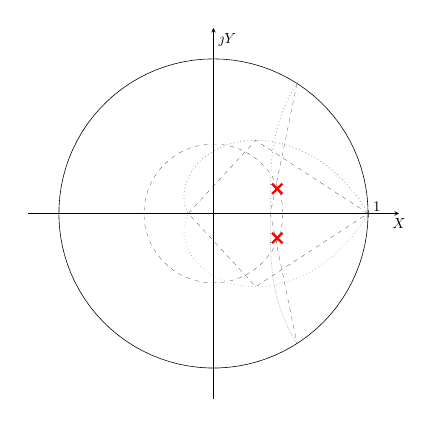
\begin{tikzpicture}[scale=0.53]

\begin{axis}[%
  axis lines=center,
  width=3.5in,
  height=3.5in,
  scale only axis,
  unbounded coords=jump,
  xmin=-1.2,
  xmax=1.2,
  ymin=-1.2,
  ymax=1.2,
  xtick={1},
  ytick=\empty,
  xticklabel style={anchor=south west, draw=none},
  xlabel={$X$},
  ylabel={$\jmath Y$},
  x label style={anchor=north}
]
\addplot [color=black!40, dotted, forget plot]
  table[row sep=crcr]{%
1	0\\
0.994975166457918	0.0086169531277774\\
0.989901329986755	0.0171473087453408\\
0.98477948302476	0.0255910797348211\\
0.979610612912339	0.0339482874654127\\
0.97439570184454	0.0422189617067992\\
0.96913572682452	0.0504031405426052\\
0.963831659617994	0.0585008702838818\\
0.958484466708655	0.0665122053826345\\
0.953095109254565	0.0744372083454012\\
0.947664543045514	0.0822759496468887\\
0.942193718461326	0.0900285076436762\\
0.936683580431134	0.0976949684879922\\
0.931135068393585	0.105275426041575\\
0.925549116258005	0.112769981789622\\
0.919926652366486	0.120178744754836\\
0.914268599456912	0.127501831411582\\
0.90857587462691	0.134739365600147\\
0.902849389298715	0.14189147844113\\
0.89709004918496	0.148958308249953\\
0.891298754255365	0.155940000451509\\
0.88547639870433	0.162836707494953\\
0.879623870919433	0.169648588768638\\
0.873742053450808	0.176375810515214\\
0.867831822981418	0.183018545746879\\
0.8618940502982	0.189576974160811\\
0.855929600264091	0.196051282054771\\
0.849939331790917	0.202441662242887\\
0.843924097813143	0.208748313971631\\
0.837884745262484	0.214971442835991\\
0.831822115043362	0.221111260695846\\
0.825737042009206	0.227167985592546\\
0.819630354939596	0.233141841665717\\
0.81350287651823	0.23903305907027\\
0.807355423311723	0.244841873893657\\
0.801188805749226	0.250568528073344\\
0.795003828102853	0.256213269314532\\
0.78880128846892	0.26177635100812\\
0.782581978749986	0.267258032148917\\
0.776346684637685	0.272658577254117\\
0.770096185596349	0.277978256282022\\
0.763831254847411	0.283217344551051\\
0.757552659354593	0.288376122659003\\
0.751261159809852	0.293454876402612\\
0.744957510620097	0.298453896697378\\
0.738642459894664	0.303373479497687\\
0.732316749433537	0.308213925717227\\
0.725981114716321	0.312975541149701\\
0.719636284891949	0.317658636389843\\
0.71328298276912	0.322263526754741\\
0.706921924807467	0.326790532205477\\
0.700553821109446	0.331239977269081\\
0.694179375412927	0.335612190960806\\
0.687799285084511	0.339907506706737\\
0.681414241113527	0.344126262266724\\
0.675024928106738	0.34826879965765\\
0.668632024283728	0.352335465077047\\
0.662236201472974	0.356326608827046\\
0.65583812510859	0.360242585238686\\
0.649438454227737	0.364083752596562\\
0.643037841468706	0.367850473063845\\
0.636636933069644	0.371543112607646\\
0.630236368867939	0.375162040924758\\
0.623836782300241	0.378707631367759\\
0.617438800403127	0.382180260871485\\
0.611043043814387	0.385580309879881\\
0.604650126774944	0.388908162273233\\
0.598260657131382	0.392164205295778\\
0.591875236339095	0.395348829483698\\
0.585494459466028	0.398462428593512\\
0.579118915197029	0.401505399530848\\
0.572749185838786	0.40447814227962\\
0.566385847325349	0.4073810598316\\
0.560029469224235	0.410214558116388\\
0.553680614743102	0.412979045931794\\
0.547339840736992	0.415674934874619\\
0.541007697716132	0.418302639271854\\
0.534684729854293	0.420862576112287\\
0.528371474997687	0.423355164978523\\
0.522068464674416	0.425780827979435\\
0.515776224104452	0.428139989683019\\
0.509495272210138	0.430433077049683\\
0.503226121627222	0.432660519365961\\
0.496969278716402	0.434822748178651\\
0.490725243575377	0.436920197229388\\
0.484494510051408	0.438953302389643\\
0.478277565754372	0.440922501596166\\
0.472074892070308	0.44282823478686\\
0.465886964175444	0.444670943837092\\
0.459714251050707	0.446451072496453\\
0.453557215496707	0.448169066325949\\
0.447416314149175	0.449825372635651\\
0.441291997494877	0.451420440422779\\
0.435184709887969	0.452954720310238\\
0.429094889566804	0.454428664485608\\
0.423022968671182	0.455842726640584\\
0.416969373260031	0.457197361910859\\
0.410934523329524	0.458493026816478\\
0.404918832831608	0.459730179202636\\
0.398922709692961	0.460909278180935\\
0.392946555834355	0.462030784071105\\
0.386990767190422	0.463095158343177\\
0.381055733729824	0.46410286356012\\
0.375141839475811	0.465054363320948\\
0.369249462527169	0.465950122204273\\
0.363378975079551	0.466790605712337\\
0.357530743447174	0.467576280215505\\
0.351705128084897	0.46830761289722\\
0.345902483610657	0.468985071699428\\
0.34012315882826	0.469609125268472\\
0.334367496750526	0.47018024290145\\
0.328635834622783	0.470698894493046\\
0.322928503946697	0.471165550482829\\
0.317245830504437	0.471580681803022\\
0.311588134383171	0.471944759826739\\
0.305955729999881	0.472258256316704\\
0.300348926126498	0.472521643374422\\
0.294768025915352	0.472735393389845\\
0.289213326924917	0.47289997899149\\
0.283685121145871	0.473015872997045\\
0.278183695027438	0.473083548364434\\
0.272709329504025	0.473103478143368\\
0.267262300022144	0.473076135427362\\
0.261842876567611	0.473001993306221\\
0.256451323693014	0.472881524819009\\
0.251087900545453	0.472715202907487\\
0.24575286089454	0.472503500370018\\
0.240446453160655	0.472246889815953\\
0.235168920443456	0.471945843620488\\
0.229920500550629	0.471600833879988\\
0.224701426026886	0.471212332367794\\
0.219511924183188	0.470780810490488\\
0.214352217126212	0.470306739244642\\
0.209222521788028	0.46979058917403\\
0.204123049956005	0.469232830327317\\
0.199054008302929	0.468633932216212\\
0.194015598417329	0.467994363774097\\
0.189008016834009	0.467314593315119\\
0.184031455064777	0.466595088493758\\
0.179086099629367	0.465836316264853\\
0.174172132086558	0.465038742844109\\
0.169289729065466	0.464202833669053\\
0.16443906229702	0.463329053360474\\
0.159620298645616	0.462417865684317\\
0.154833600140936	0.461469733514039\\
0.150079124009928	0.460485118793442\\
0.145357022708955	0.45946448249995\\
0.140667443956089	0.458408284608366\\
0.136010530763565	0.457316984055071\\
0.131386421470369	0.456191038702701\\
0.126795249774977	0.455030905305267\\
0.122237144768225	0.453837039473741\\
0.117712230966311	0.452609895642096\\
0.113220628343922	0.451349927033798\\
0.108762452367488	0.450057585628759\\
0.104337814028549	0.448733322130736\\
0.0999468198772385	0.447377585935182\\
0.0955895720558732	0.445990825097552\\
0.0912661683326492	0.444573486302051\\
0.0869767021354367	0.443126014830835\\
0.0827212625856707	0.441648854533653\\
0.0784999345323338	0.440142447797942\\
0.0743127985860244	0.438607235519351\\
0.0701599311531092	0.437043657072723\\
0.0660414044699528	0.435452150283505\\
0.0619572866372231	0.433833151399599\\
0.0579076416542657	0.432187095063656\\
0.0538925294535447	0.4305144142858\\
0.0499120059351455	0.428815540416786\\
0.045966123001336	0.42709090312159\\
0.0420549285911806	0.425340930353435\\
0.0381784667152051	0.423566048328237\\
0.0343367774901069	0.421766681499485\\
0.0305298971735083	0.419943252533545\\
0.0267578581987466	0.418096182285383\\
0.0230206892096994	0.416225889774718\\
0.0193184150956407	0.414332792162584\\
0.0156510570261221	0.412417304728323\\
0.0120186324858799	0.410479840846984\\
0.00842115530975893	0.408520811967138\\
0.00485863571765306	0.406540627589113\\
0.00133108034945763	0.404539695243628\\
-0.00216150769996924	0.402518420470845\\
-0.00561912884584125	0.400477206799821\\
-0.00904178697847668	0.39841645572837\\
-0.0124294894283334	0.396336566703324\\
-0.0157822469310498	0.394237937101194\\
-0.0191000735924938	0.39212096220923\\
-0.0223829868538259	0.389986035206885\\
-0.0256310074565762	0.387833547147654\\
-0.028844159407742	0.385663886941331\\
-0.0320224699449067	0.383477441336632\\
-0.035165969501385	0.381274594904221\\
-0.0382746916713966	0.379055730020116\\
-0.0413486731752722	0.37682122684948\\
-0.044387953824694	0.374571463330791\\
-0.0473925764879758	0.372306815160395\\
-0.0503625870553824	0.37002765577743\\
-0.053298034404496	0.367734356349131\\
-0.0561989703656271	0.365427285756506\\
-0.0590654496872782	0.363106810580375\\
-0.0618975300016593	0.360773295087786\\
-0.0646952717902602	0.358427101218792\\
-0.0674587383494818	0.356068588573591\\
-0.0701879957563293	0.353698114400028\\
-0.0728831128341696	0.351316033581455\\
-0.0755441611185572	0.348922698624945\\
-0.078171214823129	0.346518459649865\\
-0.080764350805573	0.344103664376793\\
-0.083323648533672	0.341678658116792\\
-0.0858491900514256	0.339243783761024\\
-0.0883410599452533	0.336799381770708\\
-0.0907993453102799	0.334345790167427\\
-0.0932241357167081	0.331883344523768\\
-0.0956155231762785	0.329412377954299\\
-0.0979736021088205	0.326933221106879\\
-0.100298469308897	0.324446202154309\\
-0.102590223912543	0.3219516467863\\
-0.104848967364106	0.319449878201778\\
-0.107074803383181	0.316941217101503\\
-0.109267837931654	0.314425981681024\\
-0.111428179180845	0.311904487623941\\
-0.113555937478763	0.309377048095487\\
-0.115651225317466	0.306843973736431\\
-0.117714157300535	0.304305572657284\\
-0.119744850110663	0.301762150432819\\
-0.121743422477352	0.299214010096897\\
-0.12370999514474	0.296661452137599\\
-0.125644690839534	0.294104774492655\\
-0.127547634239077	0.29154427254518\\
-0.129418951939533	0.288980239119696\\
-0.131258772424195	0.286412964478459\\
-0.133067226031924	0.283842736318072\\
-0.13484444492572	0.281269839766384\\
-0.136590563061418	0.278694557379684\\
-0.138305716156522	0.27611716914017\\
-0.139990041659173	0.273537952453705\\
-0.141643678717248	0.27095718214785\\
-0.143266768147609	0.268375130470173\\
-0.144859452405477	0.26579206708683\\
-0.146421875553965	0.263208259081419\\
-0.147954183233735	0.260623970954104\\
-0.149456522632818	0.258039464621\\
-0.150929042456566	0.255454999413824\\
-0.152371892897761	0.252870832079808\\
-0.153785225606871	0.250287216781869\\
-0.155169193662457	0.24770440509903\\
-0.156523951541726	0.245122646027102\\
-0.157849655091252	0.242542185979612\\
-0.159146461497839	0.239963268788975\\
-0.160414529259544	0.237386135707918\\
-0.161654018156862	0.234811025411143\\
-0.162865089224069	0.232238173997232\\
-0.164047904720716	0.229667814990784\\
-0.165202628103302	0.227100179344793\\
-0.166329423997092	0.224535495443257\\
-0.167428458168113	0.221973989104012\\
-0.168499897495306	0.219415883581802\\
-0.169543909942848	0.216861399571562\\
-0.170560664532644	0.214310755211935\\
-0.171550331316981	0.211764166088996\\
-0.172513081351356	0.209221845240208\\
-0.173449086667475	0.206684003158576\\
-0.174358520246424	0.204150847797023\\
-0.175241555992005	0.201622584572976\\
-0.176098368704256	0.199099416373151\\
-0.176929134053141	0.196581543558548\\
-0.177734028552409	0.194069163969646\\
-0.178513229533643	0.191562472931801\\
-0.179266915120471	0.189061663260829\\
-0.179995264202967	0.1865669252688\\
-0.180698456412218	0.184078446770007\\
-0.181376672095087	0.181596413087137\\
-0.182030092289137	0.17912100705762\\
-0.18265889869775	0.176652409040165\\
-0.183263273665422	0.17419079692148\\
-0.183843400153239	0.171736346123169\\
-0.184399461714537	0.169289229608803\\
-0.184931642470749	0.16684961789117\\
-0.185440127087425	0.164417679039694\\
-0.185925100750451	0.161993578688022\\
-0.186386749142441	0.159577480041785\\
-0.18682525841932	0.157169543886511\\
-0.18724081518709	0.154769928595712\\
-0.18763360647879	0.152378790139125\\
-0.18800381973163	0.149996282091108\\
-0.188351642764323	0.147622555639199\\
-0.1886772637546	0.145257759592815\\
-0.188980871216915	0.142902040392114\\
-0.189262653980335	0.140555542116997\\
-0.189522801166623	0.138218406496255\\
-0.189761502168506	0.135890772916862\\
-0.189978946628136	0.133572778433407\\
-0.190175324415737	0.131264557777667\\
-0.190350825608445	0.128966243368309\\
-0.190505640469335	0.126677965320734\\
-0.19063995942664	0.124399851457046\\
-0.190753973053159	0.122132027316154\\
-0.19084787204586	0.119874616163997\\
-0.190921847205665	0.117627739003896\\
-0.190976089417432	0.11539151458703\\
-0.191010789630132	0.113166059423026\\
-0.191026138837202	0.110951487790669\\
-0.191022328057108	0.108747911748734\\
-0.190999548314082	0.106555441146921\\
-0.190957990619064	0.104374183636905\\
-0.190897845950822	0.1022042446835\\
-0.190819305237275	0.100045727575919\\
-0.190722559336998	0.0978987334391491\\
-0.190607799020923	0.0957633612454201\\
-0.190475214954231	0.0936397078257795\\
-0.190324997678427	0.0915278678817618\\
-0.190157337593618	0.0894279339971549\\
-0.189972424940972	0.0873399966498598\\
-0.18977044978537	0.0852641442238417\\
-0.18955160199825	0.083200463021171\\
-0.189316071240637	0.0811490372741514\\
-0.189064046946367	0.0791099491575331\\
-0.1887957183055	0.0770832788008092\\
-0.18851127424792	0.0750691043005936\\
-0.18821090342712	0.073067501733078\\
-0.187894794204192	0.0710785451665654\\
-0.187563134631983	0.0691023066740791\\
-0.187216112439458	0.0671388563460452\\
-0.186853915016241	0.065188262303045\\
-0.186476729397344	0.0632505907086381\\
-0.186084742248091	0.0613259057822507\\
-0.185678139849218	0.0594142698121313\\
-0.185257108082164	0.0575157431683673\\
-0.184821832414555	0.0556303843159656\\
-0.18437249788586	0.0537582498279896\\
-0.183909289093245	0.0518993943987567\\
-0.183432390177603	0.0500538708570886\\
-0.182941984809774	0.0482217301796184\\
-0.182438256176944	0.0464030215041461\\
-0.181921386969236	0.044597792143048\\
-0.18139155936647	0.0428060875967306\\
-0.180848955025119	0.041027951567134\\
-0.180293755065441	0.0392634259712775\\
-0.179726140058791	0.0375125509548501\\
-0.179146290015116	0.0357753649058401\\
-0.178554384370631	0.0340519044682056\\
-0.177950601975674	0.032342204555581\\
-0.177335121082737	0.0306462983650213\\
-0.176708119334683	0.0289642173907774\\
-0.176069773753131	0.0272959914381074\\
-0.175420260727028	0.0256416486371157\\
-0.174759756001391	0.0240012154566223\\
-0.174088434666228	0.0223747167180594\\
-0.173406471145636	0.0207621756093928\\
-0.172714039187066	0.0191636136990689\\
-0.172011311850774	0.0175790509499823\\
-0.171298461499436	0.0160085057334652\\
-0.170575659787937	0.0144519948432961\\
-0.16984307765334	0.0129095335097251\\
-0.169100885305011	0.0113811354135165\\
-0.168349252214934	0.00986681270000477\\
-0.167588347108177	0.00836657599316387\\
-0.166818337953539	0.00688043440968819\\
-0.166039391954362	0.00540839557308299\\
-0.165251675539513	0.00395046562776311\\
-0.164455354354524	0.00250664925315921\\
-0.163650593252911	0.00107694967782874\\
};

\addplot [color=black!40, dotted, forget plot, each nth point=10]
  table[row sep=crcr]{%
0.54030230586814	0.841470984807897\\
0.539762693938401	0.840629664537062\\
0.539224460721023	0.83978864621053\\
0.53868760316101	0.838947930597949\\
0.538152118209836	0.838107518462474\\
0.537618002825427	0.837267410560788\\
0.537085253972145	0.836427607643129\\
0.53655386862078	0.835588110453312\\
0.536023843748535	0.83474891972876\\
0.535495176339009	0.833910036200521\\
0.534967863382191	0.833071460593297\\
0.534441901874438	0.832233193625467\\
0.533917288818469	0.831395236009111\\
0.533394021223349	0.830557588450033\\
0.532872096104475	0.829720251647789\\
0.532351510483565	0.828883226295704\\
0.531832261388641	0.828046513080903\\
0.531314345854023	0.827210112684328\\
0.530797760920307	0.826374025780767\\
0.53028250363436	0.825538253038873\\
0.529768571049302	0.82470279512119\\
0.529255960224495	0.823867652684175\\
0.528744668225529	0.823032826378221\\
0.52823469212421	0.822198316847678\\
0.527726028998549	0.821364124730882\\
0.527218675932742	0.820530250660169\\
0.526712630017168	0.819696695261905\\
0.526207888348365	0.818863459156502\\
0.525704448029027	0.818030542958447\\
0.525202306167984	0.817197947276319\\
0.524701459880193	0.816365672712812\\
0.524201906286724	0.815533719864761\\
0.523703642514747	0.814702089323156\\
0.523206665697522	0.813870781673172\\
0.522710972974383	0.813039797494186\\
0.522216561490726	0.8122091373598\\
0.521723428397999	0.811378801837861\\
0.521231570853687	0.810548791490484\\
0.5207409860213	0.809719106874073\\
0.520251671070359	0.808889748539341\\
0.519763623176388	0.808060717031331\\
0.519276839520897	0.80723201288944\\
0.518791317291371	0.806403636647435\\
0.518307053681259	0.805575588833477\\
0.51782404588996	0.80474786997014\\
0.517342291122811	0.803920480574434\\
0.516861786591075	0.803093421157821\\
0.516382529511928	0.802266692226238\\
0.515904517108448	0.80144029428012\\
0.515427746609602	0.800614227814413\\
0.514952215250233	0.799788493318601\\
0.514477920271049	0.79896309127672\\
0.514004858918611	0.798138022167384\\
0.51353302844532	0.797313286463798\\
0.513062426109404	0.796488884633783\\
0.512593049174908	0.795664817139792\\
0.512124894911682	0.794841084438931\\
0.511657960595367	0.794017686982978\\
0.511192243507383	0.793194625218402\\
0.510727740934919	0.792371899586382\\
0.510264450170919	0.791549510522827\\
0.509802368514074	0.790727458458392\\
0.509341493268803	0.7899057438185\\
0.508881821745247	0.789084367023359\\
0.508423351259256	0.788263328487982\\
0.507966079132375	0.787442628622202\\
0.507510002691835	0.786622267830696\\
0.507055119270539	0.785802246512997\\
0.506601426207052	0.784982565063518\\
0.506148920845586	0.784163223871566\\
0.505697600535993	0.78334422332136\\
0.505247462633751	0.782525563792053\\
0.504798504499949	0.781707245657746\\
0.504350723501283	0.780889269287506\\
0.503904117010036	0.780071635045386\\
0.503458682404072	0.779254343290439\\
0.503014417066823	0.77843739437674\\
0.502571318387277	0.777620788653398\\
0.502129383759965	0.776804526464577\\
0.501688610584954	0.775988608149514\\
0.501248996267831	0.775173034042531\\
0.500810538219691	0.774357804473059\\
0.500373233857132	0.773542919765647\\
0.499937080602236	0.772728380239986\\
0.499502075882562	0.771914186210922\\
0.499068217131134	0.771100337988471\\
0.498635501786428	0.770286835877842\\
0.498203927292362	0.769473680179445\\
0.497773491098285	0.768660871188913\\
0.497344190658966	0.767848409197119\\
0.49691602343458	0.767036294490186\\
0.496488986890701	0.766224527349511\\
0.496063078498286	0.765413108051773\\
0.495638295733668	0.764602036868957\\
0.495214636078543	0.763791314068363\\
0.49479209701996	0.762980939912625\\
0.494370676050306	0.762170914659728\\
0.493950370667301	0.761361238563018\\
0.493531178373981	0.760551911871226\\
0.493113096678692	0.759742934828473\\
0.492696123095076	0.758934307674296\\
0.49228025514206	0.758126030643656\\
0.491865490343845	0.757318103966953\\
0.491451826229899	0.756510527870047\\
0.491039260334939	0.755703302574268\\
0.490627790198926	0.754896428296429\\
0.490217413367051	0.754089905248849\\
0.489808127389725	0.753283733639359\\
0.48939992982257	0.75247791367132\\
0.488992818226405	0.751672445543641\\
0.488586790167236	0.750867329450786\\
0.488181843216247	0.750062565582796\\
0.487777974949788	0.749258154125298\\
0.487375182949364	0.748454095259521\\
0.486973464801624	0.747650389162311\\
0.486572818098353	0.746847036006143\\
0.486173240436456	0.746044035959138\\
0.485774729417954	0.745241389185073\\
0.485377282649968	0.744439095843398\\
0.484980897744711	0.743637156089248\\
0.484585572319477	0.742835570073457\\
0.484191303996629	0.742034337942574\\
0.483798090403591	0.74123345983887\\
0.483405929172836	0.740432935900359\\
0.483014817941875	0.739632766260805\\
0.482624754353249	0.738832951049743\\
0.482235736054514	0.738033490392481\\
0.481847760698234	0.737234384410123\\
0.481460825941973	0.736435633219578\\
0.481074929448277	0.735637236933574\\
0.480690068884672	0.734839195660667\\
0.480306241923647	0.734041509505259\\
0.479923446242647	0.733244178567608\\
0.479541679524064	0.732447202943843\\
0.479160939455223	0.73165058272597\\
0.478781223728375	0.730854318001894\\
0.478402530040683	0.730058408855422\\
0.478024856094217	0.729262855366284\\
0.477648199595939	0.728467657610137\\
0.477272558257696	0.727672815658583\\
0.476897929796208	0.726878329579179\\
0.476524311933058	0.726084199435447\\
0.476151702394684	0.725290425286892\\
0.475780098912366	0.724497007189005\\
0.475409499222216	0.723703945193283\\
0.475039901065173	0.722911239347235\\
0.474671302186985	0.722118889694397\\
0.474303700338206	0.721326896274341\\
0.47393709327418	0.720535259122689\\
0.473571478755038	0.719743978271122\\
0.473206854545681	0.718953053747392\\
0.472843218415775	0.718162485575335\\
0.472480568139739	0.71737227377488\\
0.472118901496735	0.716582418362059\\
0.471758216270658	0.715792919349022\\
0.47139851025013	0.715003776744045\\
0.471039781228482	0.71421499055154\\
0.470682027003753	0.713426560772069\\
0.470325245378674	0.712638487402353\\
0.469969434160663	0.71185077043528\\
0.46961459116181	0.71106340985992\\
0.469260714198871	0.710276405661534\\
0.468907801093259	0.709489757821582\\
0.46855584967103	0.708703466317736\\
0.468204857762879	0.70791753112389\\
0.467854823204124	0.707131952210168\\
0.467505743834703	0.706346729542938\\
0.467157617499157	0.705561863084818\\
0.46681044204663	0.704777352794687\\
0.46646421533085	0.703993198627698\\
0.466118935210123	0.703209400535282\\
0.465774599547328	0.702425958465164\\
0.465431206209898	0.701642872361368\\
0.46508875306982	0.700860142164228\\
0.46474723800362	0.700077767810399\\
0.464406658892354	0.699295749232865\\
0.464067013621601	0.698514086360948\\
0.463728300081451	0.697732779120317\\
0.463390516166498	0.696951827433\\
0.463053659775829	0.69617123121739\\
0.462717728813013	0.695390990388255\\
0.462382721186096	0.694611104856748\\
0.462048634807588	0.693831574530415\\
0.461715467594456	0.693052399313204\\
0.461383217468113	0.692273579105474\\
0.46105188235441	0.691495113804002\\
0.460721460183626	0.690717003301996\\
0.460391948890459	0.689939247489099\\
0.460063346414016	0.6891618462514\\
0.459735650697807	0.68838479947144\\
0.459408859689731	0.687608107028223\\
0.459082971342071	0.686831768797225\\
0.458757983611482	0.686055784650399\\
0.458433894458983	0.685280154456184\\
0.45811070184995	0.684504878079514\\
0.457788403754102	0.683729955381828\\
0.457466998145497	0.682955386221072\\
0.457146483002521	0.682181170451714\\
0.456826856307877	0.681407307924745\\
0.45650811604858	0.680633798487693\\
0.456190260215944	0.679860641984627\\
0.455873286805575	0.679087838256163\\
0.455557193817364	0.678315387139476\\
0.455241979255474	0.677543288468305\\
0.454927641128334	0.676771542072959\\
0.454614177448629	0.676000147780328\\
0.454301586233291	0.675229105413887\\
0.453989865503491	0.674458414793703\\
0.45367901328463	0.673688075736445\\
0.453369027606329	0.672918088055388\\
0.453059906502422	0.672148451560422\\
0.452751648010945	0.671379166058059\\
0.452444250174131	0.670610231351436\\
0.452137711038396	0.669841647240328\\
0.451832028654334	0.669073413521148\\
0.451527201076709	0.668305529986959\\
0.451223226364442	0.667537996427477\\
0.450920102580607	0.666770812629081\\
0.45061782779242	0.666003978374815\\
0.45031640007123	0.665237493444396\\
0.450015817492511	0.664471357614223\\
0.449716078135855	0.663705570657378\\
0.449417180084962	0.662940132343639\\
0.449119121427628	0.662175042439477\\
0.448821900255744	0.66141030070807\\
0.448525514665281	0.660645906909305\\
0.448229962756284	0.659881860799785\\
0.447935242632865	0.659118162132834\\
0.44764135240319	0.658354810658502\\
0.447348290179475	0.657591806123574\\
0.447056054077976	0.65682914827157\\
0.44676464221898	0.656066836842755\\
0.446474052726798	0.655304871574145\\
0.446184283729755	0.654543252199506\\
0.445895333360182	0.653781978449367\\
0.445607199754407	0.65302105005102\\
0.445319881052752	0.652260466728527\\
0.445033375399515	0.651500228202724\\
0.444747680942969	0.650740334191229\\
0.444462795835354	0.649980784408442\\
0.444178718232864	0.649221578565555\\
0.443895446295641	0.648462716370551\\
0.443612978187767	0.647704197528215\\
0.443331312077259	0.646946021740133\\
0.443050446136053	0.6461881887047\\
0.442770378540003	0.645430698117124\\
0.44249110746887	0.644673549669429\\
0.442212631106314	0.643916743050459\\
0.441934947639884	0.643160277945886\\
0.441658055261015	0.64240415403821\\
0.441381952165015	0.641648371006764\\
0.441106636551058	0.64089292852772\\
0.440832106622177	0.640137826274091\\
0.440558360585258	0.639383063915734\\
0.440285396651025	0.638628641119359\\
0.44001321303404	0.637874557548525\\
0.43974180795269	0.63712081286365\\
0.439471179629181	0.636367406722011\\
0.439201326289529	0.63561433877775\\
0.438932246163553	0.634861608681876\\
0.438663937484865	0.634109216082268\\
0.438396398490867	0.633357160623679\\
0.438129627422738	0.632605441947739\\
0.437863622525426	0.631854059692959\\
0.437598382047645	0.631103013494734\\
0.437333904241863	0.630352302985342\\
0.437070187364295	0.629601927793954\\
0.436807229674897	0.628851887546632\\
0.436545029437354	0.628102181866332\\
0.436283584919079	0.627352810372908\\
0.436022894391196	0.626603772683115\\
0.435762956128542	0.625855068410611\\
0.435503768409653	0.625106697165959\\
0.435245329516757	0.624358658556628\\
0.434987637735768	0.623610952186999\\
0.434730691356278	0.622863577658366\\
0.434474488671548	0.622116534568935\\
0.434219027978502	0.621369822513831\\
0.433964307577718	0.620623441085097\\
0.433710325773422	0.619877389871695\\
0.433457080873477	0.619131668459512\\
0.433204571189379	0.618386276431358\\
0.43295279503625	0.617641213366968\\
0.432701750732826	0.616896478843007\\
0.432451436601452	0.616152072433068\\
0.432201850968076	0.615407993707675\\
0.431952992162239	0.614664242234284\\
0.431704858517069	0.613920817577285\\
0.431457448369273	0.613177719298002\\
0.431210760059128	0.612434946954695\\
0.430964791930477	0.611692500102562\\
0.430719542330718	0.610950378293739\\
0.4304750096108	0.610208581077301\\
0.430231192125212	0.609467107999262\\
0.429988088231978	0.608725958602578\\
0.429745696292648	0.607985132427146\\
0.429504014672294	0.607244629009805\\
0.429263041739498	0.606504447884337\\
0.429022775866347	0.605764588581468\\
0.428783215428427	0.605025050628865\\
0.428544358804814	0.604285833551141\\
0.428306204378065	0.603546936869854\\
0.428068750534215	0.602808360103502\\
0.427831995662766	0.602070102767534\\
0.427595938156682	0.601332164374336\\
0.427360576412381	0.600594544433245\\
0.427125908829728	0.599857242450537\\
0.426891933812026	0.599120257929434\\
0.426658649766011	0.598383590370103\\
0.426426055101846	0.59764723926965\\
0.426194148233109	0.596911204122128\\
0.425962927576792	0.596175484418529\\
0.425732391553288	0.595440079646789\\
0.425502538586388	0.594704989291781\\
0.425273367103272	0.59397021283532\\
0.425044875534504	0.593235749756162\\
0.424817062314021	0.592501599529995\\
0.42458992587913	0.59176776162945\\
0.424363464670499	0.59103423552409\\
0.424137677132149	0.590301020680412\\
0.42391256171145	0.589568116561847\\
0.423688116859112	0.58883552262876\\
0.423464341029178	0.58810323833844\\
0.423241232679015	0.587371263145111\\
0.423018790269314	0.586639596499918\\
0.422797012264074	0.585908237850935\\
0.422575897130603	0.585177186643157\\
0.422355443339504	0.584446442318501\\
0.422135649364675	0.583716004315801\\
0.421916513683297	0.582985872070811\\
0.421698034775829	0.582256045016197\\
0.421480211126001	0.581526522581538\\
0.421263041220808	0.580797304193323\\
0.421046523550503	0.58006838927495\\
0.420830656608586	0.579339777246718\\
0.420615438891806	0.578611467525831\\
0.420400868900144	0.577883459526392\\
0.420186945136815	0.5771557526594\\
0.419973666108256	0.576428346332746\\
0.41976103032412	0.575701239951214\\
0.419549036297272	0.574974432916473\\
0.419337682543778	0.574247924627077\\
0.419126967582901	0.57352171447846\\
0.418916889937096	0.572795801862935\\
0.418707448131999	0.572070186169684\\
0.418498640696424	0.571344866784765\\
0.418290466162353	0.570619843091098\\
0.418082923064934	0.569895114468466\\
0.417876009942469	0.569170680293511\\
0.417669725336412	0.56844653993973\\
0.41746406779136	0.567722692777469\\
0.417259035855045	0.566999138173921\\
0.417054628078333	0.56627587549312\\
0.416850843015211	0.565552904095938\\
0.416647679222784	0.564830223340079\\
0.416445135261268	0.564107832580074\\
0.416243209693983	0.56338573116728\\
0.416041901087346	0.562663918449871\\
0.415841208010867	0.561942393772834\\
0.415641129037138	0.561221156477965\\
0.415441662741833	0.560500205903863\\
0.415242807703694	0.559779541385926\\
0.415044562504532	0.559059162256343\\
0.414846925729215	0.558339067844093\\
0.414649895965663	0.557619257474932\\
0.414453471804843	0.556899730471397\\
0.414257651840763	0.556180486152791\\
0.414062434670464	0.555461523835183\\
0.413867818894012	0.554742842831401\\
0.413673803114496	0.554024442451023\\
0.413480385938019	0.553306322000374\\
0.413287565973692	0.552588480782517\\
0.413095341833629	0.55187091809725\\
0.412903712132937	0.551153633241096\\
0.412712675489714	0.550436625507298\\
0.412522230525041	0.549719894185811\\
0.412332375862976	0.549003438563298\\
0.412143110130546	0.548287257923117\\
0.411954431957746	0.547571351545322\\
0.411766339977524	0.546855718706648\\
0.411578832825784	0.546140358680509\\
0.411391909141374	0.545425270736987\\
0.411205567566082	0.544710454142827\\
0.411019806744629	0.543995908161427\\
0.410834625324664	0.543281632052833\\
0.410650021956757	0.542567625073726\\
0.410465995294393	0.541853886477419\\
0.410282543993964	0.541140415513847\\
0.410099666714769	0.540427211429558\\
0.409917362119	0.539714273467703\\
0.409735628871742	0.539001600868033\\
0.409554465640962	0.538289192866882\\
0.409373871097508	0.537577048697166\\
0.409193843915101	0.536865167588369\\
0.409014382770325	0.536153548766536\\
0.408835486342629	0.535442191454261\\
0.408657153314313	0.534731094870683\\
0.408479382370527	0.534020258231471\\
0.408302172199265	0.533309680748816\\
0.408125521491354	0.532599361631423\\
0.407949428940455	0.531889300084499\\
0.407773893243052	0.531179495309743\\
0.407598913098449	0.530469946505337\\
0.407424487208762	0.529760652865935\\
0.407250614278914	0.529051613582652\\
0.40707729301663	0.528342827843053\\
0.406904522132429	0.527634294831145\\
0.406732300339621	0.526926013727362\\
0.406560626354297	0.526217983708558\\
0.40638949889533	0.525510203947991\\
0.40621891668436	0.524802673615316\\
0.406048878445796	0.524095391876573\\
0.405879382906807	0.523388357894171\\
0.405710428797317	0.522681570826882\\
0.405542014849996	0.521975029829825\\
0.40537413980026	0.521268734054456\\
0.405206802386261	0.520562682648553\\
0.405040001348882	0.519856874756209\\
0.404873735431734	0.519151309517812\\
0.404708003381144	0.518445986070039\\
0.404542803946157	0.517740903545838\\
0.404378135878525	0.51703606107442\\
0.404213997932703	0.51633145778124\\
0.404050388865844	0.515627092787988\\
0.403887307437792	0.514922965212575\\
0.403724752411077	0.514219074169115\\
0.403562722550909	0.513515418767917\\
0.403401216625174	0.512811998115469\\
0.403240233404426	0.51210881131442\\
0.403079771661883	0.511405857463572\\
0.40291983017342	0.510703135657861\\
0.402760407717566	0.510000644988341\\
0.402601503075495	0.509298384542175\\
0.402443115031024	0.508596353402615\\
0.402285242370605	0.507894550648989\\
0.402127883883318	0.507192975356682\\
0.401971038360872	0.506491626597125\\
0.401814704597591	0.505790503437778\\
0.401658881390416	0.505089604942113\\
0.401503567538893	0.504388930169596\\
0.401348761845173	0.503688478175676\\
0.401194463114003	0.502988248011761\\
0.401040670152722	0.50228823872521\\
0.400887381771257	0.501588449359308\\
0.400734596782113	0.500888878953255\\
0.400582314000372	0.500189526542143\\
0.400430532243686	0.499490391156944\\
0.400279250332273	0.49879147182449\\
0.400128467088907	0.498092767567452\\
0.399978181338919	0.497394277404329\\
0.399828391910187	0.496696000349422\\
0.399679097633134	0.495997935412819\\
0.399530297340718	0.495300081600379\\
0.399381989868431	0.494602437913709\\
0.399234174054294	0.493905003350143\\
0.399086848738846	0.49320777690273\\
0.398940012765147	0.492510757560208\\
0.398793664978765	0.491813944306987\\
0.398647804227776	0.491117336123128\\
0.398502429362755	0.490420931984323\\
0.398357539236775	0.489724730861874\\
0.398213132705398	0.489028731722674\\
0.39806920862667	0.488332933529185\\
0.397925765861118	0.487637335239415\\
0.397782803271744	0.486941935806902\\
0.39764031972402	0.486246734180684\\
0.39749831408588	0.485551729305286\\
0.397356785227718	0.484856920120692\\
0.397215732022384	0.484162305562325\\
0.397075153345175	0.483467884561025\\
0.396935048073831	0.482773656043023\\
0.396795415088531	0.482079618929922\\
0.396656253271888	0.481385772138671\\
0.396517561508943	0.480692114581542\\
0.396379338687161	0.479998645166107\\
0.396241583696423	0.479305362795214\\
0.396104295429024	0.478612266366961\\
0.395967472779668	0.477919354774671\\
0.395831114645461	0.477226626906872\\
0.395695219925906	0.476534081647265\\
0.395559787522899	0.475841717874705\\
0.395424816340726	0.475149534463171\\
0.395290305286053	0.47445753028174\\
0.395156253267925	0.473765704194565\\
0.395022659197758	0.473074055060844\\
0.39488952198934	0.472382581734794\\
0.394756840558816	0.471691283065628\\
0.394624613824694	0.47100015789752\\
0.394492840707832	0.470309205069586\\
0.394361520131436	0.46961842341585\\
0.394230651021055	0.468927811765217\\
0.394100232304577	0.468237368941446\\
0.393970262912223	0.467547093763121\\
0.393840741776541	0.466856985043618\\
0.393711667832403	0.466167041591083\\
0.393583040017001	0.465477262208394\\
0.393454857269837	0.464787645693136\\
0.393327118532725	0.464098190837569\\
0.393199822749781	0.4634088964286\\
0.393072968867421	0.462719761247745\\
0.392946555834355	0.462030784071105\\
0.392820582601581	0.461341963669332\\
0.392695048122384	0.460653298807593\\
0.392569951352326	0.459964788245545\\
0.392445291249246	0.459276430737294\\
0.392321066773252	0.458588225031369\\
0.392197276886717	0.457900169870683\\
0.392073920554277	0.457212263992505\\
0.39195099674282	0.456524506128419\\
0.391828504421489	0.455836895004296\\
0.391706442561671	0.455149429340254\\
0.391584810136995	0.454462107850625\\
0.391463606123327	0.453774929243921\\
0.391342829498766	0.453087892222794\\
0.391222479243636	0.452400995484003\\
0.391102554340488	0.451714237718375\\
0.390983053774088	0.451027617610771\\
0.390863976531415	0.450341133840043\\
0.39074532160166	0.449654785079001\\
0.390627087976215	0.448968569994374\\
0.390509274648673	0.448282487246767\\
0.390391880614822	0.447596535490627\\
0.39027490487264	0.4469107133742\\
0.39015834642229	0.446225019539494\\
0.390042204266118	0.445539452622235\\
0.389926477408644	0.444854011251828\\
0.389811164856562	0.444168694051316\\
0.389696265618732	0.443483499637336\\
0.389581778706177	0.442798426620081\\
0.389467703132079	0.442113473603252\\
0.389354037911772	0.44142863918402\\
0.389240782062742	0.440743921952978\\
0.389127934604617	0.4400593204941\\
0.389015494559166	0.439374833384694\\
0.388903460950293	0.438690459195361\\
0.388791832804034	0.438006196489943\\
0.388680609148552	0.437322043825484\\
0.38856978901413	0.436637999752179\\
0.388459371433172	0.435954062813327\\
0.388349355440191	0.435270231545288\\
0.388239740071813	0.434586504477429\\
0.388130524366765	0.433902880132079\\
0.388021707365875	0.433219357024479\\
0.387913288112068	0.432535933662733\\
0.387805265650358	0.431852608547757\\
0.387697639027846	0.43116938017323\\
0.387590407293716	0.43048624702554\\
0.387483569499229	0.429803207583734\\
0.38737712469772	0.429120260319467\\
0.387271071944593	0.428437403696945\\
0.387165410297317	0.427754636172876\\
0.387060138815421	0.427071956196414\\
0.38695525656049	0.426389362209102\\
0.386850762596162	0.425706852644822\\
0.38674665598812	0.425024425929735\\
0.386642935804091	0.424342080482224\\
0.386539601113843	0.423659814712842\\
0.386436650989175	0.422977627024248\\
0.38633408450392	0.422295515811153\\
0.386231900733932	0.421613479460259\\
0.386130098757092	0.420931516350199\\
0.386028677653294	0.42024962485148\\
0.385927636504448	0.419567803326417\\
0.385826974394472	0.418886050129075\\
0.385726690409287	0.418204363605205\\
0.385626783636818	0.417522742092183\\
0.385527253166984	0.416841183918943\\
0.385428098091694	0.416159687405916\\
0.385329317504849	0.415478250864961\\
0.385230910502332	0.414796872599304\\
0.385132876182003	0.414115550903467\\
0.385035213643701	0.413434284063202\\
0.384937921989234	0.412753070355424\\
0.384841000322377	0.412071908048142\\
0.384744447748868	0.411390795400386\\
0.384648263376404	0.410709730662142\\
0.384552446314637	0.410028712074277\\
0.384456995675168	0.409347737868467\\
0.384361910571546	0.408666806267126\\
0.384267190119259	0.407985915483331\\
0.384172833435737	0.407305063720748\\
0.384078839640342	0.406624249173555\\
0.383985207854366	0.405943470026369\\
0.383891937201027	0.405262724454166\\
0.383799026805465	0.404582010622205\\
0.383706475794738	0.403901326685946\\
0.383614283297815	0.403220670790976\\
0.38352244844558	0.40254004107292\\
0.383430970370817	0.401859435657368\\
0.383339848208215	0.401178852659787\\
0.38324908109436	0.400498290185438\\
0.383158668167731	0.399817746329295\\
0.383068608568697	0.399137219175953\\
0.382978901439512	0.39845670679955\\
0.382889545924312	0.397776207263671\\
0.382800541169111	0.397095718621266\\
0.382711886321796	0.396415238914558\\
0.382623580532124	0.39573476617495\\
0.382535622951719	0.395054298422939\\
0.382448012734064	0.394373833668017\\
0.382360749034503	0.393693369908582\\
0.382273831010232	0.393012905131842\\
0.382187257820298	0.392332437313717\\
0.382101028625594	0.391651964418743\\
0.382015142588854	0.390971484399974\\
0.381929598874653	0.390290995198883\\
0.381844396649398	0.38961049474526\\
0.381759535081328	0.388929980957112\\
0.381675013340508	0.388249451740556\\
0.381590830598827	0.38756890498972\\
0.381506986029992	0.386888338586634\\
0.381423478809526	0.386207750401122\\
0.381340308114762	0.3855271382907\\
0.381257473124843	0.384846500100458\\
0.381174973020713	0.384165833662956\\
0.381092806985117	0.383485136798108\\
0.381010974202598	0.382804407313071\\
0.380929473859488	0.382123643002129\\
0.38084830514391	0.381442841646577\\
0.380767467245771	0.380762001014603\\
0.380686959356758	0.380081118861167\\
0.380606780670337	0.379400192927887\\
0.380526930381746	0.378719220942907\\
0.380447407687995	0.378038200620784\\
0.380368211787857	0.377357129662353\\
0.380289341881869	0.376676005754608\\
0.380210797172326	0.375994826570569\\
0.380132576863278	0.375313589769156\\
0.380054680160527	0.374632292995054\\
0.37997710627162	0.373950933878582\\
0.379899854405851	0.373269510035555\\
0.379822923774251	0.372588019067155\\
0.379746313589589	0.371906458559785\\
0.379670023066367	0.371224826084931\\
0.379594051420814	0.370543119199023\\
0.379518397870887	0.369861335443291\\
0.379443061636263	0.369179472343616\\
0.379368041938338	0.368497527410386\\
0.379293338000221	0.367815498138347\\
0.379218949046733	0.367133382006451\\
0.379144874304403	0.366451176477703\\
0.379071113001461	0.365768878999008\\
0.37899766436784	0.36508648700101\\
0.378924527635168	0.364403997897939\\
0.378851702036765	0.363721409087443\\
0.378779186807642	0.363038717950432\\
0.378706981184494	0.362355921850909\\
0.378635084405699	0.361673018135801\\
0.378563495711313	0.360990004134794\\
0.378492214343068	0.360306877160158\\
0.378421239544366	0.359623634506574\\
0.378350570560279	0.358940273450957\\
0.378280206637541	0.35825679125228\\
0.378210147024547	0.357573185151387\\
0.378140390971353	0.356889452370817\\
0.378070937729664	0.356205590114612\\
0.378001786552838	0.355521595568135\\
0.37793293669588	0.35483746589787\\
0.377864387415437	0.354153198251239\\
0.377796137969796	0.353468789756396\\
0.377728187618882	0.352784237522037\\
0.377660535624252	0.352099538637192\\
0.377593181249092	0.351414690171024\\
0.377526123758214	0.350729689172624\\
0.377459362418054	0.350044532670794\\
0.377392896496666	0.349359217673844\\
0.377326725263721	0.348673741169368\\
0.377260847990499	0.347988100124031\\
0.377195263949893	0.347302291483345\\
0.377129972416399	0.346616312171444\\
0.377064972666117	0.345930159090859\\
0.377000263976743	0.345243829122282\\
0.376935845627572	0.344557319124338\\
0.376871716899487	0.343870625933344\\
0.376807877074962	0.343183746363069\\
0.376744325438057	0.342496677204488\\
0.376681061274411	0.341809415225537\\
0.376618083871243	0.341121957170863\\
0.376555392517349	0.340434299761564\\
0.376492986503093	0.339746439694935\\
0.376430865120411	0.339058373644207\\
0.376369027662802	0.338370098258277\\
0.376307473425328	0.337681610161441\\
0.37624620170461	0.33699290595312\\
0.376185211798823	0.336303982207584\\
0.376124503007693	0.335614835473666\\
0.376064074632498	0.334925462274484\\
0.376003925976059	0.334235859107143\\
0.375944056342739	0.333546022442447\\
0.375884465038442	0.332855948724598\\
0.375825151370604	0.332165634370895\\
0.375766114648197	0.331475075771423\\
0.375707354181721	0.330784269288746\\
0.3756488692832	0.33009321125759\\
0.375590659266182	0.329401897984517\\
0.375532723445736	0.328710325747605\\
0.375475061138444	0.328018490796116\\
0.375417671662403	0.327326389350157\\
0.375360554337219	0.326634017600341\\
0.375303708484006	0.325941371707444\\
0.37524713342538	0.325248447802048\\
0.375190828485456	0.32455524198419\\
0.375134792989849	0.323861750322997\\
0.375079026265665	0.323167968856317\\
0.375023527641503	0.32247389359035\\
0.374968296447448	0.321779520499264\\
0.374913332015069	0.321084845524814\\
0.374858633677417	0.32038986457595\\
0.374804200769022	0.319694573528419\\
0.374750032625887	0.318998968224362\\
0.374696128585488	0.318303044471906\\
0.374642487986769	0.317606798044745\\
0.37458911017014	0.316910224681722\\
0.374535994477473	0.316213320086395\\
0.374483140252101	0.315516079926602\\
0.37443054683881	0.314818499834022\\
0.374378213583842	0.314120575403719\\
0.374326139834889	0.313422302193687\\
0.374274324941088	0.312723675724387\\
0.374222768253021	0.312024691478272\\
0.374171469122712	0.311325344899309\\
0.37412042690362	0.310625631392488\\
0.374069640950642	0.309925546323332\\
0.374019110620105	0.309225085017387\\
0.373968835269765	0.308524242759712\\
0.373918814258803	0.307823014794359\\
0.373869046947824	0.307121396323845\\
0.37381953269885	0.306419382508609\\
0.373770270875324	0.305716968466471\\
0.373721260842097	0.305014149272069\\
0.373672501965436	0.3043109199563\\
0.373623993613012	0.303607275505741\\
0.373575735153902	0.302903210862063\\
0.373527725958584	0.30219872092144\\
0.373479965398935	0.301493800533939\\
0.373432452848228	0.300788444502909\\
0.373385187681128	0.300082647584354\\
0.37333816927369	0.299376404486292\\
0.373291397003357	0.298669709868113\\
0.373244870248953	0.297962558339916\\
0.373198588390686	0.297254944461841\\
0.37315255081014	0.296546862743382\\
0.373106756890275	0.295838307642699\\
0.373061206015423	0.295129273565906\\
0.373015897571285	0.294419754866355\\
0.372970830944928	0.2937097458439\\
0.372926005524784	0.292999240744158\\
0.372881420700642	0.292288233757746\\
0.372837075863654	0.291576719019509\\
0.372792970406321	0.290864690607737\\
0.3727491037225	0.290152142543361\\
0.372705475207395	0.28943906878914\\
0.372662084257558	0.288725463248833\\
0.372618930270881	0.28801131976635\\
0.3725760126466	0.287296632124895\\
0.372533330785286	0.286581394046088\\
0.372490884088846	0.28586559918907\\
0.372448671960518	0.285149241149599\\
0.372406693804871	0.284432313459118\\
0.372364949027797	0.283714809583816\\
0.372323437036515	0.28299672292366\\
0.372282157239562	0.282278046811424\\
0.372241109046793	0.28155877451168\\
0.37220029186938	0.280838899219789\\
0.372159705119805	0.280118414060861\\
0.372119348211861	0.279397312088694\\
0.372079220560646	0.278675586284701\\
0.372039321582563	0.277953229556813\\
0.371999650695315	0.277230234738351\\
0.371960207317906	0.276506594586892\\
0.371920990870632	0.275782301783101\\
0.371882000775084	0.275057348929544\\
0.371843236454142	0.274331728549476\\
0.371804697331975	0.273605433085609\\
0.371766382834034	0.272878454898846\\
0.371728292387053	0.272150786267004\\
0.371690425419047	0.271422419383494\\
0.371652781359303	0.270693346355991\\
0.371615359638387	0.269963559205061\\
0.371578159688132	0.269233049862775\\
0.37154118094164	0.268501810171284\\
0.37150442283328	0.267769831881368\\
0.371467884798682	0.267037106650954\\
0.371431566274738	0.266303626043605\\
0.371395466699595	0.265569381526977\\
0.371359585512659	0.264834364471242\\
0.371323922154583	0.264098566147477\\
0.371288476067274	0.263361977726022\\
0.371253246693882	0.2626245902748\\
0.371218233478804	0.261886394757605\\
0.371183435867678	0.261147382032347\\
0.37114885330738	0.260407542849263\\
0.371114485246022	0.259666867849091\\
0.371080331132951	0.258925347561198\\
0.371046390418744	0.258182972401673\\
0.371012662555207	0.257439732671377\\
0.37097914699537	0.256695618553942\\
0.370945843193489	0.255950620113742\\
0.370912750605038	0.255204727293796\\
0.370879868686711	0.254457929913647\\
0.370847196896416	0.253710217667177\\
0.370814734693273	0.252961580120379\\
0.370782481537614	0.252212006709075\\
0.370750436890978	0.251461486736587\\
0.370718600216109	0.250710009371349\\
0.370686970976953	0.249957563644464\\
0.370655548638655	0.24920413844721\\
0.37062433266756	0.248449722528478\\
0.370593322531206	0.24769430449216\\
0.370562517698324	0.246937872794467\\
0.370531917638833	0.246180415741187\\
0.370501521823841	0.24542192148488\\
0.37047132972564	0.244662378021997\\
0.370441340817705	0.243901773189943\\
0.370411554574688	0.243140094664053\\
0.370381970472421	0.242377329954507\\
0.370352587987909	0.241613466403164\\
0.37032340659933	0.240848491180316\\
0.370294425786031	0.240082391281366\\
0.370265645028525	0.23931515352342\\
0.370237063808491	0.238546764541796\\
0.370208681608771	0.23777721078644\\
0.370180497913365	0.237006478518261\\
0.37015251220743	0.236234553805359\\
0.370124723977278	0.23546142251917\\
0.370097132710374	0.234687070330501\\
0.370069737895333	0.233911482705469\\
0.370042539021915	0.233134644901329\\
0.370015535581028	0.232356541962199\\
0.36998872706472	0.231577158714665\\
0.36996211296618	0.230796479763275\\
0.369935692779735	0.230014489485909\\
0.369909466000846	0.229231172029028\\
0.369883432126107	0.228446511302792\\
0.369857590653244	0.227660490976047\\
0.369831941081108	0.226873094471176\\
0.369806482909677	0.226084304958802\\
0.369781215640053	0.225294105352357\\
0.369756138774458	0.224502478302486\\
0.369731251816231	0.223709406191306\\
0.369706554269828	0.222914871126492\\
0.369682045640819	0.222118854935208\\
0.369657725435885	0.221321339157854\\
0.369633593162815	0.22052230504164\\
0.369609648330504	0.219721733533971\\
0.369585890448953	0.218919605275644\\
0.369562319029263	0.218115900593838\\
0.369538933583636	0.21731059949491\\
0.369515733625368	0.216503681656961\\
0.369492718668853	0.215695126422198\\
0.369469888229576	0.214884912789054\\
0.369447241824111	0.214073019404076\\
0.369424778970121	0.213259424553562\\
0.369402499186354	0.212444106154945\\
0.36938040199264	0.211627041747911\\
0.369358486909892	0.210808208485241\\
0.3693367534601	0.209987583123366\\
0.369315201166329	0.209165142012623\\
0.36929382955272	0.208340861087209\\
0.369272638144484	0.207514715854803\\
0.369251626467901	0.206686681385867\\
0.369230794050319	0.205856732302592\\
0.369210140420151	0.205024842767486\\
0.369189665106871	0.204190986471587\\
0.369169367641014	0.203355136622287\\
0.369149247554172	0.202517265930751\\
0.369129304378993	0.201677346598912\\
0.36910953764918	0.200835350306022\\
0.369089946899484	0.199991248194758\\
0.369070531665707	0.199145010856834\\
0.369051291484697	0.19829660831813\\
0.369032225894347	0.197446010023291\\
0.369013334433591	0.196593184819795\\
0.368994616642403	0.195738100941449\\
0.368976072061795	0.194880725991301\\
0.368957700233815	0.194021026923938\\
0.368939500701544	0.193158970027136\\
0.368921473009093	0.192294520902846\\
0.368903616701604	0.191427644447482\\
0.368885931325242	0.190558304831462\\
0.368868416427201	0.189686465478007\\
0.368851071555694	0.188812089041114\\
0.368833896259956	0.187935137382709\\
0.368816890090237	0.187055571548916\\
0.368800052597805	0.186173351745405\\
0.368783383334942	0.185288437311783\\
0.368766881854941	0.184400786694969\\
0.368750547712102	0.183510357421519\\
0.368734380461735	0.182617106068834\\
0.368718379660153	0.181720988235212\\
0.368702544864672	0.180821958508667\\
0.36868687563361	0.179919970434472\\
0.368671371526282	0.179014976481355\\
0.368656032102999	0.178106928006267\\
0.368640856925068	0.177195775217669\\
0.368625845554786	0.176281467137245\\
0.368610997555442	0.175363951559965\\
0.36859631249131	0.174443175012407\\
0.368581789927653	0.173519082709248\\
0.368567429430716	0.172591618507822\\
0.368553230567724	0.171660724860641\\
0.368539192906884	0.170726342765767\\
0.368525316017378	0.169788411714908\\
0.368511599469366	0.16884686963912\\
0.368498042833979	0.167901652851974\\
0.368484645683318	0.166952695990042\\
0.368471407590457	0.165999931950538\\
0.368458328129432	0.165043291825968\\
0.368445406875247	0.164082704835585\\
0.368432643403868	0.163118098253477\\
0.368420037292221	0.162149397333074\\
0.368407588118192	0.161176525227855\\
0.368395295460621	0.160199402908021\\
0.368383158899307	0.159217949072881\\
0.368371178014996	0.158232080058674\\
0.368359352389388	0.157241709741542\\
0.368347681605131	0.156246749435325\\
0.368336165245818	0.155247107783853\\
0.368324802895988	0.154242690647358\\
0.368313594141121	0.153233400982614\\
0.368302538567639	0.152219138716371\\
0.368291635762899	0.151199800611629\\
0.368280885315198	0.150175280126245\\
0.368270286813765	0.149145467263324\\
0.368259839848761	0.148110248412818\\
0.36824954401128	0.147069506183681\\
0.368239398893341	0.146023119225891\\
0.368229404087892	0.144970962041572\\
0.368219559188802	0.143912904784408\\
0.368209863790866	0.142848813046427\\
0.368200317489797	0.141778547631191\\
0.368190919882227	0.140701964312307\\
0.368181670565704	0.139618913576087\\
0.368172569138691	0.138529240347058\\
0.368163615200564	0.13743278369493\\
0.368154808351608	0.136329376521432\\
0.368146148193017	0.13521884522534\\
0.368137634326893	0.134101009343784\\
0.36812926635624	0.132975681167763\\
0.368121043884968	0.131842665329573\\
0.368112966517885	0.130701758359581\\
0.3681050338607	0.129552748209534\\
0.368097245520016	0.128395413739267\\
0.368089601103335	0.127229524163301\\
0.368082100219049	0.126054838453448\\
0.368074742476442	0.124871104693086\\
0.368067527485688	0.123678059378209\\
0.368060454857847	0.122475426659834\\
0.368053524204865	0.121262917521612\\
0.368046735139573	0.120040228885755\\
0.368040087275681	0.118807042639501\\
0.368033580227781	0.11756302457331\\
0.368027213611341	0.116307823220823\\
0.368020987042707	0.115041068589238\\
0.368014900139097	0.113762370767209\\
0.368008952518604	0.112471318395502\\
0.368003143800188	0.11116747698352\\
0.367997473603679	0.109850387052287\\
0.367991941549774	0.108519562081537\\
0.367986547260036	0.107174486235047\\
0.367981290356887	0.105814611834237\\
0.367976170463614	0.104439356545167\\
0.367971187204362	0.103048100238158\\
0.367966340204131	0.101640181472294\\
0.36796162908878	0.100214893548549\\
0.367957053485019	0.0987714800650799\\
0.367952613020412	0.0973091298957599\\
0.367948307323372	0.0958269714978085\\
0.36794413602316	0.0943240664356579\\
0.367940098749883	0.0927994019850621\\
0.367936195134494	0.0912518826526587\\
0.367932424808787	0.0896803204101329\\
0.367928787405397	0.0880834233966508\\
0.367925282557801	0.0864597827854287\\
0.367921909900309	0.0848078574362777\\
0.36791866906807	0.0831259558603285\\
0.367915559697065	0.0814122148984723\\
0.367912581424107	0.079664574350939\\
0.367909733886839	0.0778807465770908\\
0.367907016723734	0.0760581797907115\\
0.367904429574089	0.0741940133758049\\
0.367901972078028	0.0722850229952613\\
0.367899643876496	0.0703275524903789\\
0.367897444611261	0.068317428466631\\
0.367895373924911	0.0662498518630737\\
0.367893431460848	0.0641192584409184\\
0.367891616863294	0.0619191365588608\\
0.367889929777284	0.059641785079356\\
0.367888369848664	0.0572779854598579\\
0.367886936724093	0.0548165476470082\\
0.367885630051037	0.0522436648106183\\
0.36788444947777	0.0495419683014623\\
0.367883394653372	0.046689092758285\\
0.367882465227726	0.0436553999892785\\
0.367881660851518	0.0404001668158235\\
0.367880981176232	0.036864741072423\\
0.367880425854153	0.0329590666840154\\
0.367879994538362	0.0285314820675801\\
0.367879686882735	0.0232861434313897\\
0.367879502541941	0.0164589265653525\\
0.367879441171442	0\\
};
\addplot [color=black!40, dotted, forget plot, each nth point=10]
  table[row sep=crcr]{%
0.54030230586814	-0.841470984807897\\
0.539762693938401	-0.840629664537062\\
0.539224460721023	-0.83978864621053\\
0.53868760316101	-0.838947930597949\\
0.538152118209836	-0.838107518462474\\
0.537618002825427	-0.837267410560788\\
0.537085253972145	-0.836427607643129\\
0.53655386862078	-0.835588110453312\\
0.536023843748535	-0.83474891972876\\
0.535495176339009	-0.833910036200521\\
0.534967863382191	-0.833071460593297\\
0.534441901874438	-0.832233193625467\\
0.533917288818469	-0.831395236009111\\
0.533394021223349	-0.830557588450033\\
0.532872096104475	-0.829720251647789\\
0.532351510483565	-0.828883226295704\\
0.531832261388641	-0.828046513080903\\
0.531314345854023	-0.827210112684328\\
0.530797760920307	-0.826374025780767\\
0.53028250363436	-0.825538253038873\\
0.529768571049302	-0.82470279512119\\
0.529255960224495	-0.823867652684175\\
0.528744668225529	-0.823032826378221\\
0.52823469212421	-0.822198316847678\\
0.527726028998549	-0.821364124730882\\
0.527218675932742	-0.820530250660169\\
0.526712630017168	-0.819696695261905\\
0.526207888348365	-0.818863459156502\\
0.525704448029027	-0.818030542958447\\
0.525202306167984	-0.817197947276319\\
0.524701459880193	-0.816365672712812\\
0.524201906286724	-0.815533719864761\\
0.523703642514747	-0.814702089323156\\
0.523206665697522	-0.813870781673172\\
0.522710972974383	-0.813039797494186\\
0.522216561490726	-0.8122091373598\\
0.521723428397999	-0.811378801837861\\
0.521231570853687	-0.810548791490484\\
0.5207409860213	-0.809719106874073\\
0.520251671070359	-0.808889748539341\\
0.519763623176388	-0.808060717031331\\
0.519276839520897	-0.80723201288944\\
0.518791317291371	-0.806403636647435\\
0.518307053681259	-0.805575588833477\\
0.51782404588996	-0.80474786997014\\
0.517342291122811	-0.803920480574434\\
0.516861786591075	-0.803093421157821\\
0.516382529511928	-0.802266692226238\\
0.515904517108448	-0.80144029428012\\
0.515427746609602	-0.800614227814413\\
0.514952215250233	-0.799788493318601\\
0.514477920271049	-0.79896309127672\\
0.514004858918611	-0.798138022167384\\
0.51353302844532	-0.797313286463798\\
0.513062426109404	-0.796488884633783\\
0.512593049174908	-0.795664817139792\\
0.512124894911682	-0.794841084438931\\
0.511657960595367	-0.794017686982978\\
0.511192243507383	-0.793194625218402\\
0.510727740934919	-0.792371899586382\\
0.510264450170919	-0.791549510522827\\
0.509802368514074	-0.790727458458392\\
0.509341493268803	-0.7899057438185\\
0.508881821745247	-0.789084367023359\\
0.508423351259256	-0.788263328487982\\
0.507966079132375	-0.787442628622202\\
0.507510002691835	-0.786622267830696\\
0.507055119270539	-0.785802246512997\\
0.506601426207052	-0.784982565063518\\
0.506148920845586	-0.784163223871566\\
0.505697600535993	-0.78334422332136\\
0.505247462633751	-0.782525563792053\\
0.504798504499949	-0.781707245657746\\
0.504350723501283	-0.780889269287506\\
0.503904117010036	-0.780071635045386\\
0.503458682404072	-0.779254343290439\\
0.503014417066823	-0.77843739437674\\
0.502571318387277	-0.777620788653398\\
0.502129383759965	-0.776804526464577\\
0.501688610584954	-0.775988608149514\\
0.501248996267831	-0.775173034042531\\
0.500810538219691	-0.774357804473059\\
0.500373233857132	-0.773542919765647\\
0.499937080602236	-0.772728380239986\\
0.499502075882562	-0.771914186210922\\
0.499068217131134	-0.771100337988471\\
0.498635501786428	-0.770286835877842\\
0.498203927292362	-0.769473680179445\\
0.497773491098285	-0.768660871188913\\
0.497344190658966	-0.767848409197119\\
0.49691602343458	-0.767036294490186\\
0.496488986890701	-0.766224527349511\\
0.496063078498286	-0.765413108051773\\
0.495638295733668	-0.764602036868957\\
0.495214636078543	-0.763791314068363\\
0.49479209701996	-0.762980939912625\\
0.494370676050306	-0.762170914659728\\
0.493950370667301	-0.761361238563018\\
0.493531178373981	-0.760551911871226\\
0.493113096678692	-0.759742934828473\\
0.492696123095076	-0.758934307674296\\
0.49228025514206	-0.758126030643656\\
0.491865490343845	-0.757318103966953\\
0.491451826229899	-0.756510527870047\\
0.491039260334939	-0.755703302574268\\
0.490627790198926	-0.754896428296429\\
0.490217413367051	-0.754089905248849\\
0.489808127389725	-0.753283733639359\\
0.48939992982257	-0.75247791367132\\
0.488992818226405	-0.751672445543641\\
0.488586790167236	-0.750867329450786\\
0.488181843216247	-0.750062565582796\\
0.487777974949788	-0.749258154125298\\
0.487375182949364	-0.748454095259521\\
0.486973464801624	-0.747650389162311\\
0.486572818098353	-0.746847036006143\\
0.486173240436456	-0.746044035959138\\
0.485774729417954	-0.745241389185073\\
0.485377282649968	-0.744439095843398\\
0.484980897744711	-0.743637156089248\\
0.484585572319477	-0.742835570073457\\
0.484191303996629	-0.742034337942574\\
0.483798090403591	-0.74123345983887\\
0.483405929172836	-0.740432935900359\\
0.483014817941875	-0.739632766260805\\
0.482624754353249	-0.738832951049743\\
0.482235736054514	-0.738033490392481\\
0.481847760698234	-0.737234384410123\\
0.481460825941973	-0.736435633219578\\
0.481074929448277	-0.735637236933574\\
0.480690068884672	-0.734839195660667\\
0.480306241923647	-0.734041509505259\\
0.479923446242647	-0.733244178567608\\
0.479541679524064	-0.732447202943843\\
0.479160939455223	-0.73165058272597\\
0.478781223728375	-0.730854318001894\\
0.478402530040683	-0.730058408855422\\
0.478024856094217	-0.729262855366284\\
0.477648199595939	-0.728467657610137\\
0.477272558257696	-0.727672815658583\\
0.476897929796208	-0.726878329579179\\
0.476524311933058	-0.726084199435447\\
0.476151702394684	-0.725290425286892\\
0.475780098912366	-0.724497007189005\\
0.475409499222216	-0.723703945193283\\
0.475039901065173	-0.722911239347235\\
0.474671302186985	-0.722118889694397\\
0.474303700338206	-0.721326896274341\\
0.47393709327418	-0.720535259122689\\
0.473571478755038	-0.719743978271122\\
0.473206854545681	-0.718953053747392\\
0.472843218415775	-0.718162485575335\\
0.472480568139739	-0.71737227377488\\
0.472118901496735	-0.716582418362059\\
0.471758216270658	-0.715792919349022\\
0.47139851025013	-0.715003776744045\\
0.471039781228482	-0.71421499055154\\
0.470682027003753	-0.713426560772069\\
0.470325245378674	-0.712638487402353\\
0.469969434160663	-0.71185077043528\\
0.46961459116181	-0.71106340985992\\
0.469260714198871	-0.710276405661534\\
0.468907801093259	-0.709489757821582\\
0.46855584967103	-0.708703466317736\\
0.468204857762879	-0.70791753112389\\
0.467854823204124	-0.707131952210168\\
0.467505743834703	-0.706346729542938\\
0.467157617499157	-0.705561863084818\\
0.46681044204663	-0.704777352794687\\
0.46646421533085	-0.703993198627698\\
0.466118935210123	-0.703209400535282\\
0.465774599547328	-0.702425958465164\\
0.465431206209898	-0.701642872361368\\
0.46508875306982	-0.700860142164228\\
0.46474723800362	-0.700077767810399\\
0.464406658892354	-0.699295749232865\\
0.464067013621601	-0.698514086360948\\
0.463728300081451	-0.697732779120317\\
0.463390516166498	-0.696951827433\\
0.463053659775829	-0.69617123121739\\
0.462717728813013	-0.695390990388255\\
0.462382721186096	-0.694611104856748\\
0.462048634807588	-0.693831574530415\\
0.461715467594456	-0.693052399313204\\
0.461383217468113	-0.692273579105474\\
0.46105188235441	-0.691495113804002\\
0.460721460183626	-0.690717003301996\\
0.460391948890459	-0.689939247489099\\
0.460063346414016	-0.6891618462514\\
0.459735650697807	-0.68838479947144\\
0.459408859689731	-0.687608107028223\\
0.459082971342071	-0.686831768797225\\
0.458757983611482	-0.686055784650399\\
0.458433894458983	-0.685280154456184\\
0.45811070184995	-0.684504878079514\\
0.457788403754102	-0.683729955381828\\
0.457466998145497	-0.682955386221072\\
0.457146483002521	-0.682181170451714\\
0.456826856307877	-0.681407307924745\\
0.45650811604858	-0.680633798487693\\
0.456190260215944	-0.679860641984627\\
0.455873286805575	-0.679087838256163\\
0.455557193817364	-0.678315387139476\\
0.455241979255474	-0.677543288468305\\
0.454927641128334	-0.676771542072959\\
0.454614177448629	-0.676000147780328\\
0.454301586233291	-0.675229105413887\\
0.453989865503491	-0.674458414793703\\
0.45367901328463	-0.673688075736445\\
0.453369027606329	-0.672918088055388\\
0.453059906502422	-0.672148451560422\\
0.452751648010945	-0.671379166058059\\
0.452444250174131	-0.670610231351436\\
0.452137711038396	-0.669841647240328\\
0.451832028654334	-0.669073413521148\\
0.451527201076709	-0.668305529986959\\
0.451223226364442	-0.667537996427477\\
0.450920102580607	-0.666770812629081\\
0.45061782779242	-0.666003978374815\\
0.45031640007123	-0.665237493444396\\
0.450015817492511	-0.664471357614223\\
0.449716078135855	-0.663705570657378\\
0.449417180084962	-0.662940132343639\\
0.449119121427628	-0.662175042439477\\
0.448821900255744	-0.66141030070807\\
0.448525514665281	-0.660645906909305\\
0.448229962756284	-0.659881860799785\\
0.447935242632865	-0.659118162132834\\
0.44764135240319	-0.658354810658502\\
0.447348290179475	-0.657591806123574\\
0.447056054077976	-0.65682914827157\\
0.44676464221898	-0.656066836842755\\
0.446474052726798	-0.655304871574145\\
0.446184283729755	-0.654543252199506\\
0.445895333360182	-0.653781978449367\\
0.445607199754407	-0.65302105005102\\
0.445319881052752	-0.652260466728527\\
0.445033375399515	-0.651500228202724\\
0.444747680942969	-0.650740334191229\\
0.444462795835354	-0.649980784408442\\
0.444178718232864	-0.649221578565555\\
0.443895446295641	-0.648462716370551\\
0.443612978187767	-0.647704197528215\\
0.443331312077259	-0.646946021740133\\
0.443050446136053	-0.6461881887047\\
0.442770378540003	-0.645430698117124\\
0.44249110746887	-0.644673549669429\\
0.442212631106314	-0.643916743050459\\
0.441934947639884	-0.643160277945886\\
0.441658055261015	-0.64240415403821\\
0.441381952165015	-0.641648371006764\\
0.441106636551058	-0.64089292852772\\
0.440832106622177	-0.640137826274091\\
0.440558360585258	-0.639383063915734\\
0.440285396651025	-0.638628641119359\\
0.44001321303404	-0.637874557548525\\
0.43974180795269	-0.63712081286365\\
0.439471179629181	-0.636367406722011\\
0.439201326289529	-0.63561433877775\\
0.438932246163553	-0.634861608681876\\
0.438663937484865	-0.634109216082268\\
0.438396398490867	-0.633357160623679\\
0.438129627422738	-0.632605441947739\\
0.437863622525426	-0.631854059692959\\
0.437598382047645	-0.631103013494734\\
0.437333904241863	-0.630352302985342\\
0.437070187364295	-0.629601927793954\\
0.436807229674897	-0.628851887546632\\
0.436545029437354	-0.628102181866332\\
0.436283584919079	-0.627352810372908\\
0.436022894391196	-0.626603772683115\\
0.435762956128542	-0.625855068410611\\
0.435503768409653	-0.625106697165959\\
0.435245329516757	-0.624358658556628\\
0.434987637735768	-0.623610952186999\\
0.434730691356278	-0.622863577658366\\
0.434474488671548	-0.622116534568935\\
0.434219027978502	-0.621369822513831\\
0.433964307577718	-0.620623441085097\\
0.433710325773422	-0.619877389871695\\
0.433457080873477	-0.619131668459512\\
0.433204571189379	-0.618386276431358\\
0.43295279503625	-0.617641213366968\\
0.432701750732826	-0.616896478843007\\
0.432451436601452	-0.616152072433068\\
0.432201850968076	-0.615407993707675\\
0.431952992162239	-0.614664242234284\\
0.431704858517069	-0.613920817577285\\
0.431457448369273	-0.613177719298002\\
0.431210760059128	-0.612434946954695\\
0.430964791930477	-0.611692500102562\\
0.430719542330718	-0.610950378293739\\
0.4304750096108	-0.610208581077301\\
0.430231192125212	-0.609467107999262\\
0.429988088231978	-0.608725958602578\\
0.429745696292648	-0.607985132427146\\
0.429504014672294	-0.607244629009805\\
0.429263041739498	-0.606504447884337\\
0.429022775866347	-0.605764588581468\\
0.428783215428427	-0.605025050628865\\
0.428544358804814	-0.604285833551141\\
0.428306204378065	-0.603546936869854\\
0.428068750534215	-0.602808360103502\\
0.427831995662766	-0.602070102767534\\
0.427595938156682	-0.601332164374336\\
0.427360576412381	-0.600594544433245\\
0.427125908829728	-0.599857242450537\\
0.426891933812026	-0.599120257929434\\
0.426658649766011	-0.598383590370103\\
0.426426055101846	-0.59764723926965\\
0.426194148233109	-0.596911204122128\\
0.425962927576792	-0.596175484418529\\
0.425732391553288	-0.595440079646789\\
0.425502538586388	-0.594704989291781\\
0.425273367103272	-0.59397021283532\\
0.425044875534504	-0.593235749756162\\
0.424817062314021	-0.592501599529995\\
0.42458992587913	-0.59176776162945\\
0.424363464670499	-0.59103423552409\\
0.424137677132149	-0.590301020680412\\
0.42391256171145	-0.589568116561847\\
0.423688116859112	-0.58883552262876\\
0.423464341029178	-0.58810323833844\\
0.423241232679015	-0.587371263145111\\
0.423018790269314	-0.586639596499918\\
0.422797012264074	-0.585908237850935\\
0.422575897130603	-0.585177186643157\\
0.422355443339504	-0.584446442318501\\
0.422135649364675	-0.583716004315801\\
0.421916513683297	-0.582985872070811\\
0.421698034775829	-0.582256045016197\\
0.421480211126001	-0.581526522581538\\
0.421263041220808	-0.580797304193323\\
0.421046523550503	-0.58006838927495\\
0.420830656608586	-0.579339777246718\\
0.420615438891806	-0.578611467525831\\
0.420400868900144	-0.577883459526392\\
0.420186945136815	-0.5771557526594\\
0.419973666108256	-0.576428346332746\\
0.41976103032412	-0.575701239951214\\
0.419549036297272	-0.574974432916473\\
0.419337682543778	-0.574247924627077\\
0.419126967582901	-0.57352171447846\\
0.418916889937096	-0.572795801862935\\
0.418707448131999	-0.572070186169684\\
0.418498640696424	-0.571344866784765\\
0.418290466162353	-0.570619843091098\\
0.418082923064934	-0.569895114468466\\
0.417876009942469	-0.569170680293511\\
0.417669725336412	-0.56844653993973\\
0.41746406779136	-0.567722692777469\\
0.417259035855045	-0.566999138173921\\
0.417054628078333	-0.56627587549312\\
0.416850843015211	-0.565552904095938\\
0.416647679222784	-0.564830223340079\\
0.416445135261268	-0.564107832580074\\
0.416243209693983	-0.56338573116728\\
0.416041901087346	-0.562663918449871\\
0.415841208010867	-0.561942393772834\\
0.415641129037138	-0.561221156477965\\
0.415441662741833	-0.560500205903863\\
0.415242807703694	-0.559779541385926\\
0.415044562504532	-0.559059162256343\\
0.414846925729215	-0.558339067844093\\
0.414649895965663	-0.557619257474932\\
0.414453471804843	-0.556899730471397\\
0.414257651840763	-0.556180486152791\\
0.414062434670464	-0.555461523835183\\
0.413867818894012	-0.554742842831401\\
0.413673803114496	-0.554024442451023\\
0.413480385938019	-0.553306322000374\\
0.413287565973692	-0.552588480782517\\
0.413095341833629	-0.55187091809725\\
0.412903712132937	-0.551153633241096\\
0.412712675489714	-0.550436625507298\\
0.412522230525041	-0.549719894185811\\
0.412332375862976	-0.549003438563298\\
0.412143110130546	-0.548287257923117\\
0.411954431957746	-0.547571351545322\\
0.411766339977524	-0.546855718706648\\
0.411578832825784	-0.546140358680509\\
0.411391909141374	-0.545425270736987\\
0.411205567566082	-0.544710454142827\\
0.411019806744629	-0.543995908161427\\
0.410834625324664	-0.543281632052833\\
0.410650021956757	-0.542567625073726\\
0.410465995294393	-0.541853886477419\\
0.410282543993964	-0.541140415513847\\
0.410099666714769	-0.540427211429558\\
0.409917362119	-0.539714273467703\\
0.409735628871742	-0.539001600868033\\
0.409554465640962	-0.538289192866882\\
0.409373871097508	-0.537577048697166\\
0.409193843915101	-0.536865167588369\\
0.409014382770325	-0.536153548766536\\
0.408835486342629	-0.535442191454261\\
0.408657153314313	-0.534731094870683\\
0.408479382370527	-0.534020258231471\\
0.408302172199265	-0.533309680748816\\
0.408125521491354	-0.532599361631423\\
0.407949428940455	-0.531889300084499\\
0.407773893243052	-0.531179495309743\\
0.407598913098449	-0.530469946505337\\
0.407424487208762	-0.529760652865935\\
0.407250614278914	-0.529051613582652\\
0.40707729301663	-0.528342827843053\\
0.406904522132429	-0.527634294831145\\
0.406732300339621	-0.526926013727362\\
0.406560626354297	-0.526217983708558\\
0.40638949889533	-0.525510203947991\\
0.40621891668436	-0.524802673615316\\
0.406048878445796	-0.524095391876573\\
0.405879382906807	-0.523388357894171\\
0.405710428797317	-0.522681570826882\\
0.405542014849996	-0.521975029829825\\
0.40537413980026	-0.521268734054456\\
0.405206802386261	-0.520562682648553\\
0.405040001348882	-0.519856874756209\\
0.404873735431734	-0.519151309517812\\
0.404708003381144	-0.518445986070039\\
0.404542803946157	-0.517740903545838\\
0.404378135878525	-0.51703606107442\\
0.404213997932703	-0.51633145778124\\
0.404050388865844	-0.515627092787988\\
0.403887307437792	-0.514922965212575\\
0.403724752411077	-0.514219074169115\\
0.403562722550909	-0.513515418767917\\
0.403401216625174	-0.512811998115469\\
0.403240233404426	-0.51210881131442\\
0.403079771661883	-0.511405857463572\\
0.40291983017342	-0.510703135657861\\
0.402760407717566	-0.510000644988341\\
0.402601503075495	-0.509298384542175\\
0.402443115031024	-0.508596353402615\\
0.402285242370605	-0.507894550648989\\
0.402127883883318	-0.507192975356682\\
0.401971038360872	-0.506491626597125\\
0.401814704597591	-0.505790503437778\\
0.401658881390416	-0.505089604942113\\
0.401503567538893	-0.504388930169596\\
0.401348761845173	-0.503688478175676\\
0.401194463114003	-0.502988248011761\\
0.401040670152722	-0.50228823872521\\
0.400887381771257	-0.501588449359308\\
0.400734596782113	-0.500888878953255\\
0.400582314000372	-0.500189526542143\\
0.400430532243686	-0.499490391156944\\
0.400279250332273	-0.49879147182449\\
0.400128467088907	-0.498092767567452\\
0.399978181338919	-0.497394277404329\\
0.399828391910187	-0.496696000349422\\
0.399679097633134	-0.495997935412819\\
0.399530297340718	-0.495300081600379\\
0.399381989868431	-0.494602437913709\\
0.399234174054294	-0.493905003350143\\
0.399086848738846	-0.49320777690273\\
0.398940012765147	-0.492510757560208\\
0.398793664978765	-0.491813944306987\\
0.398647804227776	-0.491117336123128\\
0.398502429362755	-0.490420931984323\\
0.398357539236775	-0.489724730861874\\
0.398213132705398	-0.489028731722674\\
0.39806920862667	-0.488332933529185\\
0.397925765861118	-0.487637335239415\\
0.397782803271744	-0.486941935806902\\
0.39764031972402	-0.486246734180684\\
0.39749831408588	-0.485551729305286\\
0.397356785227718	-0.484856920120692\\
0.397215732022384	-0.484162305562325\\
0.397075153345175	-0.483467884561025\\
0.396935048073831	-0.482773656043023\\
0.396795415088531	-0.482079618929922\\
0.396656253271888	-0.481385772138671\\
0.396517561508943	-0.480692114581542\\
0.396379338687161	-0.479998645166107\\
0.396241583696423	-0.479305362795214\\
0.396104295429024	-0.478612266366961\\
0.395967472779668	-0.477919354774671\\
0.395831114645461	-0.477226626906872\\
0.395695219925906	-0.476534081647265\\
0.395559787522899	-0.475841717874705\\
0.395424816340726	-0.475149534463171\\
0.395290305286053	-0.47445753028174\\
0.395156253267925	-0.473765704194565\\
0.395022659197758	-0.473074055060844\\
0.39488952198934	-0.472382581734794\\
0.394756840558816	-0.471691283065628\\
0.394624613824694	-0.47100015789752\\
0.394492840707832	-0.470309205069586\\
0.394361520131436	-0.46961842341585\\
0.394230651021055	-0.468927811765217\\
0.394100232304577	-0.468237368941446\\
0.393970262912223	-0.467547093763121\\
0.393840741776541	-0.466856985043618\\
0.393711667832403	-0.466167041591083\\
0.393583040017001	-0.465477262208394\\
0.393454857269837	-0.464787645693136\\
0.393327118532725	-0.464098190837569\\
0.393199822749781	-0.4634088964286\\
0.393072968867421	-0.462719761247745\\
0.392946555834355	-0.462030784071105\\
0.392820582601581	-0.461341963669332\\
0.392695048122384	-0.460653298807593\\
0.392569951352326	-0.459964788245545\\
0.392445291249246	-0.459276430737294\\
0.392321066773252	-0.458588225031369\\
0.392197276886717	-0.457900169870683\\
0.392073920554277	-0.457212263992505\\
0.39195099674282	-0.456524506128419\\
0.391828504421489	-0.455836895004296\\
0.391706442561671	-0.455149429340254\\
0.391584810136995	-0.454462107850625\\
0.391463606123327	-0.453774929243921\\
0.391342829498766	-0.453087892222794\\
0.391222479243636	-0.452400995484003\\
0.391102554340488	-0.451714237718375\\
0.390983053774088	-0.451027617610771\\
0.390863976531415	-0.450341133840043\\
0.39074532160166	-0.449654785079001\\
0.390627087976215	-0.448968569994374\\
0.390509274648673	-0.448282487246767\\
0.390391880614822	-0.447596535490627\\
0.39027490487264	-0.4469107133742\\
0.39015834642229	-0.446225019539494\\
0.390042204266118	-0.445539452622235\\
0.389926477408644	-0.444854011251828\\
0.389811164856562	-0.444168694051316\\
0.389696265618732	-0.443483499637336\\
0.389581778706177	-0.442798426620081\\
0.389467703132079	-0.442113473603252\\
0.389354037911772	-0.44142863918402\\
0.389240782062742	-0.440743921952978\\
0.389127934604617	-0.4400593204941\\
0.389015494559166	-0.439374833384694\\
0.388903460950293	-0.438690459195361\\
0.388791832804034	-0.438006196489943\\
0.388680609148552	-0.437322043825484\\
0.38856978901413	-0.436637999752179\\
0.388459371433172	-0.435954062813327\\
0.388349355440191	-0.435270231545288\\
0.388239740071813	-0.434586504477429\\
0.388130524366765	-0.433902880132079\\
0.388021707365875	-0.433219357024479\\
0.387913288112068	-0.432535933662733\\
0.387805265650358	-0.431852608547757\\
0.387697639027846	-0.43116938017323\\
0.387590407293716	-0.43048624702554\\
0.387483569499229	-0.429803207583734\\
0.38737712469772	-0.429120260319467\\
0.387271071944593	-0.428437403696945\\
0.387165410297317	-0.427754636172876\\
0.387060138815421	-0.427071956196414\\
0.38695525656049	-0.426389362209102\\
0.386850762596162	-0.425706852644822\\
0.38674665598812	-0.425024425929735\\
0.386642935804091	-0.424342080482224\\
0.386539601113843	-0.423659814712842\\
0.386436650989175	-0.422977627024248\\
0.38633408450392	-0.422295515811153\\
0.386231900733932	-0.421613479460259\\
0.386130098757092	-0.420931516350199\\
0.386028677653294	-0.42024962485148\\
0.385927636504448	-0.419567803326417\\
0.385826974394472	-0.418886050129075\\
0.385726690409287	-0.418204363605205\\
0.385626783636818	-0.417522742092183\\
0.385527253166984	-0.416841183918943\\
0.385428098091694	-0.416159687405916\\
0.385329317504849	-0.415478250864961\\
0.385230910502332	-0.414796872599304\\
0.385132876182003	-0.414115550903467\\
0.385035213643701	-0.413434284063202\\
0.384937921989234	-0.412753070355424\\
0.384841000322377	-0.412071908048142\\
0.384744447748868	-0.411390795400386\\
0.384648263376404	-0.410709730662142\\
0.384552446314637	-0.410028712074277\\
0.384456995675168	-0.409347737868467\\
0.384361910571546	-0.408666806267126\\
0.384267190119259	-0.407985915483331\\
0.384172833435737	-0.407305063720748\\
0.384078839640342	-0.406624249173555\\
0.383985207854366	-0.405943470026369\\
0.383891937201027	-0.405262724454166\\
0.383799026805465	-0.404582010622205\\
0.383706475794738	-0.403901326685946\\
0.383614283297815	-0.403220670790976\\
0.38352244844558	-0.40254004107292\\
0.383430970370817	-0.401859435657368\\
0.383339848208215	-0.401178852659787\\
0.38324908109436	-0.400498290185438\\
0.383158668167731	-0.399817746329295\\
0.383068608568697	-0.399137219175953\\
0.382978901439512	-0.39845670679955\\
0.382889545924312	-0.397776207263671\\
0.382800541169111	-0.397095718621266\\
0.382711886321796	-0.396415238914558\\
0.382623580532124	-0.39573476617495\\
0.382535622951719	-0.395054298422939\\
0.382448012734064	-0.394373833668017\\
0.382360749034503	-0.393693369908582\\
0.382273831010232	-0.393012905131842\\
0.382187257820298	-0.392332437313717\\
0.382101028625594	-0.391651964418743\\
0.382015142588854	-0.390971484399974\\
0.381929598874653	-0.390290995198883\\
0.381844396649398	-0.38961049474526\\
0.381759535081328	-0.388929980957112\\
0.381675013340508	-0.388249451740556\\
0.381590830598827	-0.38756890498972\\
0.381506986029992	-0.386888338586634\\
0.381423478809526	-0.386207750401122\\
0.381340308114762	-0.3855271382907\\
0.381257473124843	-0.384846500100458\\
0.381174973020713	-0.384165833662956\\
0.381092806985117	-0.383485136798108\\
0.381010974202598	-0.382804407313071\\
0.380929473859488	-0.382123643002129\\
0.38084830514391	-0.381442841646577\\
0.380767467245771	-0.380762001014603\\
0.380686959356758	-0.380081118861167\\
0.380606780670337	-0.379400192927887\\
0.380526930381746	-0.378719220942907\\
0.380447407687995	-0.378038200620784\\
0.380368211787857	-0.377357129662353\\
0.380289341881869	-0.376676005754608\\
0.380210797172326	-0.375994826570569\\
0.380132576863278	-0.375313589769156\\
0.380054680160527	-0.374632292995054\\
0.37997710627162	-0.373950933878582\\
0.379899854405851	-0.373269510035555\\
0.379822923774251	-0.372588019067155\\
0.379746313589589	-0.371906458559785\\
0.379670023066367	-0.371224826084931\\
0.379594051420814	-0.370543119199023\\
0.379518397870887	-0.369861335443291\\
0.379443061636263	-0.369179472343616\\
0.379368041938338	-0.368497527410386\\
0.379293338000221	-0.367815498138347\\
0.379218949046733	-0.367133382006451\\
0.379144874304403	-0.366451176477703\\
0.379071113001461	-0.365768878999008\\
0.37899766436784	-0.36508648700101\\
0.378924527635168	-0.364403997897939\\
0.378851702036765	-0.363721409087443\\
0.378779186807642	-0.363038717950432\\
0.378706981184494	-0.362355921850909\\
0.378635084405699	-0.361673018135801\\
0.378563495711313	-0.360990004134794\\
0.378492214343068	-0.360306877160158\\
0.378421239544366	-0.359623634506574\\
0.378350570560279	-0.358940273450957\\
0.378280206637541	-0.35825679125228\\
0.378210147024547	-0.357573185151387\\
0.378140390971353	-0.356889452370817\\
0.378070937729664	-0.356205590114612\\
0.378001786552838	-0.355521595568135\\
0.37793293669588	-0.35483746589787\\
0.377864387415437	-0.354153198251239\\
0.377796137969796	-0.353468789756396\\
0.377728187618882	-0.352784237522037\\
0.377660535624252	-0.352099538637192\\
0.377593181249092	-0.351414690171024\\
0.377526123758214	-0.350729689172624\\
0.377459362418054	-0.350044532670794\\
0.377392896496666	-0.349359217673844\\
0.377326725263721	-0.348673741169368\\
0.377260847990499	-0.347988100124031\\
0.377195263949893	-0.347302291483345\\
0.377129972416399	-0.346616312171444\\
0.377064972666117	-0.345930159090859\\
0.377000263976743	-0.345243829122282\\
0.376935845627572	-0.344557319124338\\
0.376871716899487	-0.343870625933344\\
0.376807877074962	-0.343183746363069\\
0.376744325438057	-0.342496677204488\\
0.376681061274411	-0.341809415225537\\
0.376618083871243	-0.341121957170863\\
0.376555392517349	-0.340434299761564\\
0.376492986503093	-0.339746439694935\\
0.376430865120411	-0.339058373644207\\
0.376369027662802	-0.338370098258277\\
0.376307473425328	-0.337681610161441\\
0.37624620170461	-0.33699290595312\\
0.376185211798823	-0.336303982207584\\
0.376124503007693	-0.335614835473666\\
0.376064074632498	-0.334925462274484\\
0.376003925976059	-0.334235859107143\\
0.375944056342739	-0.333546022442447\\
0.375884465038442	-0.332855948724598\\
0.375825151370604	-0.332165634370895\\
0.375766114648197	-0.331475075771423\\
0.375707354181721	-0.330784269288746\\
0.3756488692832	-0.33009321125759\\
0.375590659266182	-0.329401897984517\\
0.375532723445736	-0.328710325747605\\
0.375475061138444	-0.328018490796116\\
0.375417671662403	-0.327326389350157\\
0.375360554337219	-0.326634017600341\\
0.375303708484006	-0.325941371707444\\
0.37524713342538	-0.325248447802048\\
0.375190828485456	-0.32455524198419\\
0.375134792989849	-0.323861750322997\\
0.375079026265665	-0.323167968856317\\
0.375023527641503	-0.32247389359035\\
0.374968296447448	-0.321779520499264\\
0.374913332015069	-0.321084845524814\\
0.374858633677417	-0.32038986457595\\
0.374804200769022	-0.319694573528419\\
0.374750032625887	-0.318998968224362\\
0.374696128585488	-0.318303044471906\\
0.374642487986769	-0.317606798044745\\
0.37458911017014	-0.316910224681722\\
0.374535994477473	-0.316213320086395\\
0.374483140252101	-0.315516079926602\\
0.37443054683881	-0.314818499834022\\
0.374378213583842	-0.314120575403719\\
0.374326139834889	-0.313422302193687\\
0.374274324941088	-0.312723675724387\\
0.374222768253021	-0.312024691478272\\
0.374171469122712	-0.311325344899309\\
0.37412042690362	-0.310625631392488\\
0.374069640950642	-0.309925546323332\\
0.374019110620105	-0.309225085017387\\
0.373968835269765	-0.308524242759712\\
0.373918814258803	-0.307823014794359\\
0.373869046947824	-0.307121396323845\\
0.37381953269885	-0.306419382508609\\
0.373770270875324	-0.305716968466471\\
0.373721260842097	-0.305014149272069\\
0.373672501965436	-0.3043109199563\\
0.373623993613012	-0.303607275505741\\
0.373575735153902	-0.302903210862063\\
0.373527725958584	-0.30219872092144\\
0.373479965398935	-0.301493800533939\\
0.373432452848228	-0.300788444502909\\
0.373385187681128	-0.300082647584354\\
0.37333816927369	-0.299376404486292\\
0.373291397003357	-0.298669709868113\\
0.373244870248953	-0.297962558339916\\
0.373198588390686	-0.297254944461841\\
0.37315255081014	-0.296546862743382\\
0.373106756890275	-0.295838307642699\\
0.373061206015423	-0.295129273565906\\
0.373015897571285	-0.294419754866355\\
0.372970830944928	-0.2937097458439\\
0.372926005524784	-0.292999240744158\\
0.372881420700642	-0.292288233757746\\
0.372837075863654	-0.291576719019509\\
0.372792970406321	-0.290864690607737\\
0.3727491037225	-0.290152142543361\\
0.372705475207395	-0.28943906878914\\
0.372662084257558	-0.288725463248833\\
0.372618930270881	-0.28801131976635\\
0.3725760126466	-0.287296632124895\\
0.372533330785286	-0.286581394046088\\
0.372490884088846	-0.28586559918907\\
0.372448671960518	-0.285149241149599\\
0.372406693804871	-0.284432313459118\\
0.372364949027797	-0.283714809583816\\
0.372323437036515	-0.28299672292366\\
0.372282157239562	-0.282278046811424\\
0.372241109046793	-0.28155877451168\\
0.37220029186938	-0.280838899219789\\
0.372159705119805	-0.280118414060861\\
0.372119348211861	-0.279397312088694\\
0.372079220560646	-0.278675586284701\\
0.372039321582563	-0.277953229556813\\
0.371999650695315	-0.277230234738351\\
0.371960207317906	-0.276506594586892\\
0.371920990870632	-0.275782301783101\\
0.371882000775084	-0.275057348929544\\
0.371843236454142	-0.274331728549476\\
0.371804697331975	-0.273605433085609\\
0.371766382834034	-0.272878454898846\\
0.371728292387053	-0.272150786267004\\
0.371690425419047	-0.271422419383494\\
0.371652781359303	-0.270693346355991\\
0.371615359638387	-0.269963559205061\\
0.371578159688132	-0.269233049862775\\
0.37154118094164	-0.268501810171284\\
0.37150442283328	-0.267769831881368\\
0.371467884798682	-0.267037106650954\\
0.371431566274738	-0.266303626043605\\
0.371395466699595	-0.265569381526977\\
0.371359585512659	-0.264834364471242\\
0.371323922154583	-0.264098566147477\\
0.371288476067274	-0.263361977726022\\
0.371253246693882	-0.2626245902748\\
0.371218233478804	-0.261886394757605\\
0.371183435867678	-0.261147382032347\\
0.37114885330738	-0.260407542849263\\
0.371114485246022	-0.259666867849091\\
0.371080331132951	-0.258925347561198\\
0.371046390418744	-0.258182972401673\\
0.371012662555207	-0.257439732671377\\
0.37097914699537	-0.256695618553942\\
0.370945843193489	-0.255950620113742\\
0.370912750605038	-0.255204727293796\\
0.370879868686711	-0.254457929913647\\
0.370847196896416	-0.253710217667177\\
0.370814734693273	-0.252961580120379\\
0.370782481537614	-0.252212006709075\\
0.370750436890978	-0.251461486736587\\
0.370718600216109	-0.250710009371349\\
0.370686970976953	-0.249957563644464\\
0.370655548638655	-0.24920413844721\\
0.37062433266756	-0.248449722528478\\
0.370593322531206	-0.24769430449216\\
0.370562517698324	-0.246937872794467\\
0.370531917638833	-0.246180415741187\\
0.370501521823841	-0.24542192148488\\
0.37047132972564	-0.244662378021997\\
0.370441340817705	-0.243901773189943\\
0.370411554574688	-0.243140094664053\\
0.370381970472421	-0.242377329954507\\
0.370352587987909	-0.241613466403164\\
0.37032340659933	-0.240848491180316\\
0.370294425786031	-0.240082391281366\\
0.370265645028525	-0.23931515352342\\
0.370237063808491	-0.238546764541796\\
0.370208681608771	-0.23777721078644\\
0.370180497913365	-0.237006478518261\\
0.37015251220743	-0.236234553805359\\
0.370124723977278	-0.23546142251917\\
0.370097132710374	-0.234687070330501\\
0.370069737895333	-0.233911482705469\\
0.370042539021915	-0.233134644901329\\
0.370015535581028	-0.232356541962199\\
0.36998872706472	-0.231577158714665\\
0.36996211296618	-0.230796479763275\\
0.369935692779735	-0.230014489485909\\
0.369909466000846	-0.229231172029028\\
0.369883432126107	-0.228446511302792\\
0.369857590653244	-0.227660490976047\\
0.369831941081108	-0.226873094471176\\
0.369806482909677	-0.226084304958802\\
0.369781215640053	-0.225294105352357\\
0.369756138774458	-0.224502478302486\\
0.369731251816231	-0.223709406191306\\
0.369706554269828	-0.222914871126492\\
0.369682045640819	-0.222118854935208\\
0.369657725435885	-0.221321339157854\\
0.369633593162815	-0.22052230504164\\
0.369609648330504	-0.219721733533971\\
0.369585890448953	-0.218919605275644\\
0.369562319029263	-0.218115900593838\\
0.369538933583636	-0.21731059949491\\
0.369515733625368	-0.216503681656961\\
0.369492718668853	-0.215695126422198\\
0.369469888229576	-0.214884912789054\\
0.369447241824111	-0.214073019404076\\
0.369424778970121	-0.213259424553562\\
0.369402499186354	-0.212444106154945\\
0.36938040199264	-0.211627041747911\\
0.369358486909892	-0.210808208485241\\
0.3693367534601	-0.209987583123366\\
0.369315201166329	-0.209165142012623\\
0.36929382955272	-0.208340861087209\\
0.369272638144484	-0.207514715854803\\
0.369251626467901	-0.206686681385867\\
0.369230794050319	-0.205856732302592\\
0.369210140420151	-0.205024842767486\\
0.369189665106871	-0.204190986471587\\
0.369169367641014	-0.203355136622287\\
0.369149247554172	-0.202517265930751\\
0.369129304378993	-0.201677346598912\\
0.36910953764918	-0.200835350306022\\
0.369089946899484	-0.199991248194758\\
0.369070531665707	-0.199145010856834\\
0.369051291484697	-0.19829660831813\\
0.369032225894347	-0.197446010023291\\
0.369013334433591	-0.196593184819795\\
0.368994616642403	-0.195738100941449\\
0.368976072061795	-0.194880725991301\\
0.368957700233815	-0.194021026923938\\
0.368939500701544	-0.193158970027136\\
0.368921473009093	-0.192294520902846\\
0.368903616701604	-0.191427644447482\\
0.368885931325242	-0.190558304831462\\
0.368868416427201	-0.189686465478007\\
0.368851071555694	-0.188812089041114\\
0.368833896259956	-0.187935137382709\\
0.368816890090237	-0.187055571548916\\
0.368800052597805	-0.186173351745405\\
0.368783383334942	-0.185288437311783\\
0.368766881854941	-0.184400786694969\\
0.368750547712102	-0.183510357421519\\
0.368734380461735	-0.182617106068834\\
0.368718379660153	-0.181720988235212\\
0.368702544864672	-0.180821958508667\\
0.36868687563361	-0.179919970434472\\
0.368671371526282	-0.179014976481355\\
0.368656032102999	-0.178106928006267\\
0.368640856925068	-0.177195775217669\\
0.368625845554786	-0.176281467137245\\
0.368610997555442	-0.175363951559965\\
0.36859631249131	-0.174443175012407\\
0.368581789927653	-0.173519082709248\\
0.368567429430716	-0.172591618507822\\
0.368553230567724	-0.171660724860641\\
0.368539192906884	-0.170726342765767\\
0.368525316017378	-0.169788411714908\\
0.368511599469366	-0.16884686963912\\
0.368498042833979	-0.167901652851974\\
0.368484645683318	-0.166952695990042\\
0.368471407590457	-0.165999931950538\\
0.368458328129432	-0.165043291825968\\
0.368445406875247	-0.164082704835585\\
0.368432643403868	-0.163118098253477\\
0.368420037292221	-0.162149397333074\\
0.368407588118192	-0.161176525227855\\
0.368395295460621	-0.160199402908021\\
0.368383158899307	-0.159217949072881\\
0.368371178014996	-0.158232080058674\\
0.368359352389388	-0.157241709741542\\
0.368347681605131	-0.156246749435325\\
0.368336165245818	-0.155247107783853\\
0.368324802895988	-0.154242690647358\\
0.368313594141121	-0.153233400982614\\
0.368302538567639	-0.152219138716371\\
0.368291635762899	-0.151199800611629\\
0.368280885315198	-0.150175280126245\\
0.368270286813765	-0.149145467263324\\
0.368259839848761	-0.148110248412818\\
0.36824954401128	-0.147069506183681\\
0.368239398893341	-0.146023119225891\\
0.368229404087892	-0.144970962041572\\
0.368219559188802	-0.143912904784408\\
0.368209863790866	-0.142848813046427\\
0.368200317489797	-0.141778547631191\\
0.368190919882227	-0.140701964312307\\
0.368181670565704	-0.139618913576087\\
0.368172569138691	-0.138529240347058\\
0.368163615200564	-0.13743278369493\\
0.368154808351608	-0.136329376521432\\
0.368146148193017	-0.13521884522534\\
0.368137634326893	-0.134101009343784\\
0.36812926635624	-0.132975681167763\\
0.368121043884968	-0.131842665329573\\
0.368112966517885	-0.130701758359581\\
0.3681050338607	-0.129552748209534\\
0.368097245520016	-0.128395413739267\\
0.368089601103335	-0.127229524163301\\
0.368082100219049	-0.126054838453448\\
0.368074742476442	-0.124871104693086\\
0.368067527485688	-0.123678059378209\\
0.368060454857847	-0.122475426659834\\
0.368053524204865	-0.121262917521612\\
0.368046735139573	-0.120040228885755\\
0.368040087275681	-0.118807042639501\\
0.368033580227781	-0.11756302457331\\
0.368027213611341	-0.116307823220823\\
0.368020987042707	-0.115041068589238\\
0.368014900139097	-0.113762370767209\\
0.368008952518604	-0.112471318395502\\
0.368003143800188	-0.11116747698352\\
0.367997473603679	-0.109850387052287\\
0.367991941549774	-0.108519562081537\\
0.367986547260036	-0.107174486235047\\
0.367981290356887	-0.105814611834237\\
0.367976170463614	-0.104439356545167\\
0.367971187204362	-0.103048100238158\\
0.367966340204131	-0.101640181472294\\
0.36796162908878	-0.100214893548549\\
0.367957053485019	-0.0987714800650799\\
0.367952613020412	-0.0973091298957599\\
0.367948307323372	-0.0958269714978085\\
0.36794413602316	-0.0943240664356579\\
0.367940098749883	-0.0927994019850621\\
0.367936195134494	-0.0912518826526587\\
0.367932424808787	-0.0896803204101329\\
0.367928787405397	-0.0880834233966508\\
0.367925282557801	-0.0864597827854287\\
0.367921909900309	-0.0848078574362777\\
0.36791866906807	-0.0831259558603285\\
0.367915559697065	-0.0814122148984723\\
0.367912581424107	-0.079664574350939\\
0.367909733886839	-0.0778807465770908\\
0.367907016723734	-0.0760581797907115\\
0.367904429574089	-0.0741940133758049\\
0.367901972078028	-0.0722850229952613\\
0.367899643876496	-0.0703275524903789\\
0.367897444611261	-0.068317428466631\\
0.367895373924911	-0.0662498518630737\\
0.367893431460848	-0.0641192584409184\\
0.367891616863294	-0.0619191365588608\\
0.367889929777284	-0.059641785079356\\
0.367888369848664	-0.0572779854598579\\
0.367886936724093	-0.0548165476470082\\
0.367885630051037	-0.0522436648106183\\
0.36788444947777	-0.0495419683014623\\
0.367883394653372	-0.046689092758285\\
0.367882465227726	-0.0436553999892785\\
0.367881660851518	-0.0404001668158235\\
0.367880981176232	-0.036864741072423\\
0.367880425854153	-0.0329590666840154\\
0.367879994538362	-0.0285314820675801\\
0.367879686882735	-0.0232861434313897\\
0.367879502541941	-0.0164589265653525\\
0.367879441171442	-0\\
};
\addplot [ultra thin, color=black, dashed, forget plot]
  table[row sep=crcr]{%
0.449328964117222	0\\
0.447084190876696	0.0448580456862023\\
0.440372300187315	0.0892678846080065\\
0.429260355042192	0.132785788334847\\
0.413859382324095	0.174976940357792\\
0.394323263461539	0.215419780632368\\
0.370847196896416	0.253710217667177\\
0.343665747725689	0.289465666072504\\
0.31305050400448	0.322328869227062\\
0.279307363127997	0.351971468868062\\
0.242773475405877	0.37809728593843\\
0.203813875367744	0.400445279910048\\
0.162817834458846	0.418792157014416\\
0.120194971568456	0.432954601320177\\
0.076371160253329	0.442791106365311\\
0.0317842735498999	0.448203389042922\\
-0.0131201911083558	0.449137371613558\\
-0.0578935631540154	0.445583722032109\\
-0.102088481853708	0.43757794719051\\
-0.145263366188683	0.425200038144622\\
-0.186986826986386	0.408573670870039\\
-0.226841977218468	0.387864970532621\\
-0.264430597398172	0.363280851620755\\
-0.299377114457807	0.335066950524179\\
-0.331332354350697	0.303505171216372\\
-0.359977030882829	0.268910868563243\\
-0.385024935914966	0.231629697401545\\
-0.406225799059764	0.192034158870009\\
-0.423367788300752	0.150519878501097\\
-0.436279626547824	0.107501653261459\\
-0.4448323029813	0.0634093070377541\\
-0.448940362085397	0.0186833959784583\\
-0.44856275749149	-0.0262291933975447\\
-0.443703262099863	-0.070879709343338\\
-0.434410430382131	-0.114822018663089\\
-0.420777113241018	-0.157617064327472\\
-0.402939530274822	-0.19883725238637\\
-0.38107590871622	-0.23807072434628\\
-0.355404702644674	-0.27492547232424\\
-0.326182410265477	-0.309033255861015\\
-0.293701011064477	-0.34005328125804\\
-0.258285048445567	-0.367675606675404\\
-0.220288387000275	-0.391624238968265\\
-0.180090676809735	-0.411659891319117\\
-0.138093560106576	-0.427582374112576\\
-0.0947166581984938	-0.439232595163844\\
-0.050393378750857	-0.446494149315227\\
-0.00556658532057788	-0.449294481517995\\
0.0393158275901564	-0.447605611778445\\
0.0838054097476945	-0.441444414724749\\
0.127457635953419	-0.430872451001246\\
0.169836347592589	-0.415995352174835\\
0.210518110587047	-0.396961765299273\\
0.249096446208555	-0.373961867682955\\
0.285185892479884	-0.347225466700107\\
0.318425855583477	-0.317019703631471\\
0.348484212795674	-0.283646384476931\\
0.375060630947181	-0.247438964409727\\
0.397889567252825	-0.208759216002587\\
0.416742922527284	-0.167993614515772\\
0.431432320276745	-0.125549476364021\\
0.441810988894565	-0.0818508893455798\\
0.447775228154646	-0.0373344752971042\\
0.449328964117222	0\\
};

\addplot [color=black, forget plot]
  table[row sep=crcr]{%
0	1\\
0.0634239196565645	0.997986676471884\\
0.126592453573749	0.991954812830795\\
0.18925124436041	0.981928697262707\\
0.251147987181079	0.967948701396356\\
0.312033445698487	0.950071117740945\\
0.371662455660328	0.928367933016073\\
0.429794912089172	0.902926538286621\\
0.486196736100469	0.873849377069785\\
0.540640817455598	0.841253532831181\\
0.59290792905464	0.805270257531059\\
0.642787609686539	0.766044443118978\\
0.690079011482112	0.72373403810507\\
0.734591708657533	0.678509411557132\\
0.776146464291757	0.630552667084523\\
0.814575952050336	0.580056909571198\\
0.849725429949514	0.527225467610502\\
0.881453363447582	0.472271074772683\\
0.909631995354518	0.415415013001886\\
0.934147860265107	0.356886221591872\\
0.954902241444074	0.296920375328275\\
0.971811568323542	0.235758935509427\\
0.984807753012208	0.173648177666931\\
0.993838464461254	0.110838199901011\\
0.998867339183008	0.0475819158237424\\
0.999874127673875	-0.015865963834808\\
0.996854775951942	-0.0792499568567885\\
0.989821441880933	-0.142314838273285\\
0.978802446214779	-0.204806668065191\\
0.963842158559942	-0.266473813690035\\
0.945000818714669	-0.327067963317421\\
0.922354294104581	-0.386345125693128\\
0.895993774291336	-0.444066612605774\\
0.866025403784439	-0.5\\
0.832569854634771	-0.55392006386611\\
0.795761840530832	-0.605609687137666\\
0.755749574354258	-0.654860733945285\\
0.712694171378863	-0.701474887706321\\
0.666769000516292	-0.745264449675755\\
0.618158986220605	-0.786053094742787\\
0.567059863862771	-0.823676581429833\\
0.513677391573407	-0.857983413234977\\
0.458226521727411	-0.888835448654923\\
0.400930535406614	-0.916108457432069\\
0.342020143325669	-0.939692620785908\\
0.28173255684143	-0.959492973614497\\
0.220310532786541	-0.975429786885407\\
0.15800139597335	-0.987438888676394\\
0.0950560433041829	-0.995471922573085\\
0.0317279334980681	-0.999496542383185\\
-0.0317279334980679	-0.999496542383185\\
-0.0950560433041826	-0.995471922573085\\
-0.15800139597335	-0.987438888676394\\
-0.220310532786541	-0.975429786885407\\
-0.281732556841429	-0.959492973614497\\
-0.342020143325669	-0.939692620785908\\
-0.400930535406613	-0.91610845743207\\
-0.45822652172741	-0.888835448654924\\
-0.513677391573406	-0.857983413234977\\
-0.567059863862771	-0.823676581429833\\
-0.618158986220605	-0.786053094742788\\
-0.666769000516292	-0.745264449675755\\
-0.712694171378863	-0.701474887706322\\
-0.755749574354258	-0.654860733945285\\
-0.795761840530832	-0.605609687137667\\
-0.832569854634771	-0.55392006386611\\
-0.866025403784438	-0.5\\
-0.895993774291336	-0.444066612605774\\
-0.922354294104581	-0.386345125693129\\
-0.945000818714668	-0.327067963317422\\
-0.963842158559942	-0.266473813690035\\
-0.978802446214779	-0.204806668065191\\
-0.989821441880933	-0.142314838273285\\
-0.996854775951942	-0.0792499568567888\\
-0.999874127673875	-0.0158659638348076\\
-0.998867339183008	0.0475819158237424\\
-0.993838464461254	0.110838199901011\\
-0.984807753012208	0.17364817766693\\
-0.971811568323542	0.235758935509427\\
-0.954902241444074	0.296920375328275\\
-0.934147860265107	0.356886221591872\\
-0.909631995354519	0.415415013001886\\
-0.881453363447582	0.472271074772682\\
-0.849725429949514	0.527225467610502\\
-0.814575952050336	0.580056909571198\\
-0.776146464291757	0.630552667084522\\
-0.734591708657534	0.678509411557132\\
-0.690079011482113	0.723734038105069\\
-0.64278760968654	0.766044443118977\\
-0.59290792905464	0.805270257531059\\
-0.540640817455597	0.841253532831181\\
-0.486196736100469	0.873849377069785\\
-0.429794912089172	0.902926538286621\\
-0.371662455660328	0.928367933016072\\
-0.312033445698487	0.950071117740945\\
-0.251147987181079	0.967948701396356\\
-0.189251244360411	0.981928697262707\\
-0.12659245357375	0.991954812830795\\
-0.0634239196565654	0.997986676471884\\
-2.44929359829471e-16	1\\
};
\addplot [color=black!40, dotted, forget plot]
  table[row sep=crcr]{%
1	0\\
0.981351289648387	0.0311519321337182\\
0.962079910818889	0.0611419775489267\\
0.942233670491796	0.0899724066083356\\
0.921859413382688	0.117646936615124\\
0.901002994812432	0.144170674852961\\
0.879709255857547	0.169550061843105\\
0.858022000731623	0.193792814885573\\
0.83598397634735	0.216907871948577\\
0.813636854007647	0.238905335967671\\
0.791021213173413	0.259796419613294\\
0.768176527254584	0.279593390582649\\
0.745141151370439	0.298309517469198\\
0.721952312024421	0.315959016260318\\
0.698646098638223	0.332556997511064\\
0.675257456889377	0.348119414239343\\
0.651820183796266	0.362663010585226\\
0.628366924494154	0.376205271274587\\
0.604929170645636	0.388764371924752\\
0.581537260428816	0.40035913022736\\
0.558220380046452	0.411008958041233\\
0.535006566699347	0.420733814425669\\
0.511922712967412	0.429554159642228\\
0.488994572541939	0.437490910150799\\
0.466246767252958	0.444565394623516\\
0.44370279533577	0.450799310997861\\
0.42138504088122	0.456214684588197\\
0.399314784414626	0.460833827272855\\
0.377512214548836	0.464679297771893\\
0.355996440657385	0.467773863028629\\
0.334785506514365	0.470140460706157\\
0.313896404848227	0.471802162808162\\
0.293345092757459	0.472782140431538\\
0.273146507936801	0.473103629656554\\
0.253314585663456	0.472789898578602\\
0.233862276493551	0.47186421548391\\
0.214801564619969	0.470349818170023\\
0.196143486843559	0.468269884410295\\
0.177898152110645	0.465647503560165\\
0.160074761570704	0.462505649301585\\
0.142681629109065	0.458867153520547\\
0.125726202310449	0.454754681311407\\
0.109215083810249	0.450190707100395\\
0.093154052991423	0.445197491879528\\
0.0775480879859746	0.439797061540971\\
0.0624013879410696	0.434011186300842\\
0.0477173955108997	0.427861361200348\\
0.03349881953653	0.421368787671229\\
0.0197476578770711	0.4145543561515\\
0.00646522035663016	0.407438629736617\\
-0.00634784820737035	0.40004182885038\\
-0.0186915449277906	0.392383816919069\\
-0.0305664857554402	0.38448408703162\\
-0.0419738824018239	0.376361749567943\\
-0.0529155193068476	0.368035520776854\\
-0.0633937306802272	0.359523712284514\\
-0.0734113776442131	0.35084422151373\\
-0.0829718255041162	0.342014522993968\\
-0.0920789211719995	0.333051660541494\\
-0.100736970767785	0.323972240288636\\
-0.108950717420918	0.314792424540815\\
-0.116725319294638	0.305527926439655\\
-0.124066327853817	0.2961940054102\\
-0.130979666396236	0.286805463370039\\
-0.137471608866144	0.277376641677919\\
-0.143548758967859	0.267921418799253\\
-0.149218029596137	0.258453208665826\\
-0.15448662259906	0.248984959706866\\
-0.159362008888116	0.239529154528612\\
-0.163851908909233	0.230097810219465\\
-0.1679642734875	0.220702479257822\\
-0.171707265057395	0.211354250999688\\
-0.175089239289387	0.202063753723278\\
-0.178118727122867	0.192841157207846\\
-0.180804417214481	0.183696175824131\\
-0.183155138810053	0.174638072113946\\
-0.185179845047432	0.165675660836576\\
-0.186887596696776	0.156817313459873\\
-0.188287546343963	0.14807096307411\\
-0.189388923022037	0.139444109706925\\
-0.190201017294832	0.130943826017902\\
-0.190733166796158	0.122576763351629\\
-0.190994742227231	0.114349158128363\\
-0.190995133814317	0.106266838551717\\
-0.190743738227874	0.0983352316131303\\
-0.190249945963844	0.0905593703732119\\
-0.189523129187093	0.0829439015003882\\
-0.188572630036398	0.0754930930476686\\
-0.187407749389793	0.0682108424487047\\
-0.18603773608852	0.0611006847147154\\
-0.184471776617292	0.0541658008142453\\
-0.182718985238043	0.047409026218129\\
-0.180788394573871	0.0408328595924578\\
-0.178688946639379	0.0344394716227609\\
-0.17642948431318	0.0282307139530498\\
-0.174018743247891	0.0222081282238091\\
-0.171465344212555	0.0163729551934586\\
-0.16877778586201	0.0107261439282618\\
-0.165964437927393	0.00526836104610135\\
-0.16303353482158	1.99658496572927e-17\\
-0.16303353482158	-1.99658496572927e-17\\
-0.165964437927393	-0.00526836104610135\\
-0.16877778586201	-0.0107261439282618\\
-0.171465344212555	-0.0163729551934586\\
-0.174018743247891	-0.0222081282238091\\
-0.17642948431318	-0.0282307139530498\\
-0.178688946639379	-0.0344394716227609\\
-0.180788394573871	-0.0408328595924578\\
-0.182718985238043	-0.047409026218129\\
-0.184471776617292	-0.0541658008142453\\
-0.18603773608852	-0.0611006847147154\\
-0.187407749389793	-0.0682108424487047\\
-0.188572630036398	-0.0754930930476686\\
-0.189523129187093	-0.0829439015003882\\
-0.190249945963844	-0.0905593703732119\\
-0.190743738227874	-0.0983352316131303\\
-0.190995133814317	-0.106266838551717\\
-0.190994742227231	-0.114349158128363\\
-0.190733166796158	-0.122576763351629\\
-0.190201017294832	-0.130943826017902\\
-0.189388923022037	-0.139444109706925\\
-0.188287546343963	-0.14807096307411\\
-0.186887596696776	-0.156817313459873\\
-0.185179845047432	-0.165675660836576\\
-0.183155138810053	-0.174638072113946\\
-0.180804417214481	-0.183696175824131\\
-0.178118727122867	-0.192841157207846\\
-0.175089239289387	-0.202063753723278\\
-0.171707265057395	-0.211354250999688\\
-0.1679642734875	-0.220702479257822\\
-0.163851908909233	-0.230097810219465\\
-0.159362008888116	-0.239529154528612\\
-0.15448662259906	-0.248984959706866\\
-0.149218029596137	-0.258453208665826\\
-0.143548758967859	-0.267921418799253\\
-0.137471608866144	-0.277376641677919\\
-0.130979666396236	-0.286805463370039\\
-0.124066327853817	-0.2961940054102\\
-0.116725319294638	-0.305527926439655\\
-0.108950717420918	-0.314792424540815\\
-0.100736970767785	-0.323972240288636\\
-0.0920789211719995	-0.333051660541494\\
-0.0829718255041162	-0.342014522993968\\
-0.0734113776442131	-0.35084422151373\\
-0.0633937306802272	-0.359523712284514\\
-0.0529155193068476	-0.368035520776854\\
-0.0419738824018239	-0.376361749567943\\
-0.0305664857554402	-0.38448408703162\\
-0.0186915449277906	-0.392383816919069\\
-0.00634784820737035	-0.40004182885038\\
0.00646522035663016	-0.407438629736617\\
0.0197476578770711	-0.4145543561515\\
0.03349881953653	-0.421368787671229\\
0.0477173955108997	-0.427861361200348\\
0.0624013879410696	-0.434011186300842\\
0.0775480879859746	-0.439797061540971\\
0.093154052991423	-0.445197491879528\\
0.109215083810249	-0.450190707100395\\
0.125726202310449	-0.454754681311407\\
0.142681629109065	-0.458867153520547\\
0.160074761570704	-0.462505649301585\\
0.177898152110645	-0.465647503560165\\
0.196143486843559	-0.468269884410295\\
0.214801564619969	-0.470349818170023\\
0.233862276493551	-0.47186421548391\\
0.253314585663456	-0.472789898578602\\
0.273146507936801	-0.473103629656554\\
0.293345092757459	-0.472782140431538\\
0.313896404848227	-0.471802162808162\\
0.334785506514365	-0.470140460706157\\
0.355996440657385	-0.467773863028629\\
0.377512214548836	-0.464679297771893\\
0.399314784414626	-0.460833827272855\\
0.42138504088122	-0.456214684588197\\
0.44370279533577	-0.450799310997861\\
0.466246767252958	-0.444565394623516\\
0.488994572541939	-0.437490910150799\\
0.511922712967412	-0.429554159642228\\
0.535006566699347	-0.420733814425669\\
0.558220380046452	-0.411008958041233\\
0.581537260428816	-0.40035913022736\\
0.604929170645636	-0.388764371924752\\
0.628366924494154	-0.376205271274587\\
0.651820183796266	-0.362663010585226\\
0.675257456889377	-0.348119414239343\\
0.698646098638223	-0.332556997511064\\
0.721952312024421	-0.315959016260318\\
0.745141151370439	-0.298309517469198\\
0.768176527254584	-0.279593390582649\\
0.791021213173413	-0.259796419613294\\
0.813636854007647	-0.238905335967671\\
0.83598397634735	-0.216907871948577\\
0.858022000731623	-0.193792814885573\\
0.879709255857547	-0.169550061843105\\
0.901002994812432	-0.144170674852961\\
0.921859413382688	-0.117646936615124\\
0.942233670491796	-0.0899724066083356\\
0.962079910818889	-0.0611419775489267\\
0.981351289648387	-0.0311519321337182\\
1	0\\
nan	0\\
};

\addplot [color=black!40, dotted, forget plot]
  table[row sep=crcr]{%
0.54030230586814	0.841470984807897\\
0.523839075837643	0.814928316186227\\
0.508687320595882	0.788736271322035\\
0.494768449644869	0.762935534189694\\
0.482005752907937	0.7375600143713\\
0.47032474799982	0.712637387522045\\
0.459653461283272	0.688189626551107\\
0.44992264841671	0.664233518320049\\
0.441065960151734	0.640781161632712\\
0.433020059085366	0.617840443185288\\
0.425724692928414	0.595415488957203\\
0.419122729635893	0.573507089249993\\
0.413160159474338	0.55211309622246\\
0.407786068788665	0.53122879332768\\
0.402952589891059	0.510847236534364\\
0.398614831137396	0.490959567616075\\
0.394730790892751	0.471555300122364\\
0.391261258724557	0.452622578911893\\
0.388169706806669	0.434148414335319\\
0.385422174175058	0.416118892311548\\
0.382987146150303	0.39851936165114\\
0.380835430936167	0.381334600051309\\
0.378940035119482	0.36454896022382\\
0.377276039535394	0.34814649762556\\
0.375820476724226	0.332111081246612\\
0.374552210991787	0.316426488876725\\
0.373451821893269	0.301076488222204\\
0.372501491791189	0.286044905184962\\
0.371684897988954	0.271315680546931\\
0.370987109812263	0.256872916228713\\
0.370394490899359	0.242700912213813\\
0.369894606866539	0.22878419515056\\
0.369476138435956	0.215107539564813\\
0.369128800046965	0.201655982538708\\
0.368843263918867	0.188414832635262\\
0.368611089490272	0.175369673776221\\
0.368424658127448	0.162506364711798\\
0.368277112969447	0.149811034656222\\
0.368162303760724	0.137270075602611\\
0.368074736511088	0.124870131774795\\
0.368009527817544	0.112598086622262\\
0.367962363681836	0.100441047717563\\
0.367929462660766	0.0883863298730892\\
0.367907543192914	0.0764214367560594\\
0.367893794954673	0.0645340412467305\\
0.367885854110147	0.0527119647551002\\
0.367881782332874	0.0409431556855508\\
0.367880049492378	0.0292156672168579\\
0.367879519914666	0.0175176345466192\\
0.367879442142994	0.00583725173430473\\
0.367879442142994	-0.00583725173430464\\
0.367879519914666	-0.0175176345466191\\
0.367880049492378	-0.0292156672168578\\
0.367881782332874	-0.0409431556855508\\
0.367885854110147	-0.0527119647551001\\
0.367893794954673	-0.0645340412467302\\
0.367907543192914	-0.0764214367560592\\
0.367929462660766	-0.0883863298730889\\
0.367962363681836	-0.100441047717563\\
0.368009527817544	-0.112598086622262\\
0.368074736511088	-0.124870131774795\\
0.368162303760724	-0.137270075602611\\
0.368277112969447	-0.149811034656221\\
0.368424658127448	-0.162506364711798\\
0.368611089490272	-0.175369673776221\\
0.368843263918867	-0.188414832635262\\
0.369128800046965	-0.201655982538708\\
0.369476138435956	-0.215107539564813\\
0.369894606866539	-0.22878419515056\\
0.370394490899359	-0.242700912213813\\
0.370987109812263	-0.256872916228713\\
0.371684897988954	-0.271315680546931\\
0.372501491791189	-0.286044905184962\\
0.373451821893269	-0.301076488222203\\
0.374552210991787	-0.316426488876726\\
0.375820476724225	-0.332111081246612\\
0.377276039535394	-0.34814649762556\\
0.378940035119482	-0.36454896022382\\
0.380835430936167	-0.381334600051309\\
0.382987146150303	-0.39851936165114\\
0.385422174175058	-0.416118892311548\\
0.388169706806669	-0.43414841433532\\
0.391261258724557	-0.452622578911893\\
0.394730790892751	-0.471555300122364\\
0.398614831137396	-0.490959567616075\\
0.402952589891059	-0.510847236534364\\
0.407786068788665	-0.53122879332768\\
0.413160159474337	-0.552113096222459\\
0.419122729635893	-0.573507089249993\\
0.425724692928414	-0.595415488957203\\
0.433020059085366	-0.617840443185288\\
0.441065960151734	-0.640781161632711\\
0.44992264841671	-0.664233518320049\\
0.459653461283271	-0.688189626551107\\
0.47032474799982	-0.712637387522044\\
0.482005752907937	-0.7375600143713\\
0.494768449644869	-0.762935534189693\\
0.508687320595882	-0.788736271322035\\
0.523839075837643	-0.814928316186226\\
0.54030230586814	-0.841470984807896\\
nan	0\\
};

\addplot [ultra thin, color=black, dashed, forget plot]
  table[row sep=crcr]{%
0.54030230586814	0.841470984807897\\
0.367879441171442	0\\
0.54030230586814	-0.841470984807897\\
};

\addplot [color=red, only marks, mark size=5pt, mark=x, mark options={solid, red, ultra thick}, forget plot]
  table[row sep=crcr]{%
0.412479396742007	0.159164696234069\\
0.412479396742007	-0.159164696234069\\
};

\draw[ultra thin, black, dashed] (1,0) -- (0.2731, 0.4731) -- (-0.1630,0) -- (0.2731, -0.4731) -- (1,0);
\end{axis}
\end{tikzpicture}%
      \caption{}
      \label{subfig:TesteC}
  \end{subfigure}
  \begin{subfigure}[t]{0.3\columnwidth}
    % This file was created by matlab2tikz.
%
%The latest updates can be retrieved from
%  http://www.mathworks.com/matlabcentral/fileexchange/22022-matlab2tikz-matlab2tikz
%where you can also make suggestions and rate matlab2tikz.
%
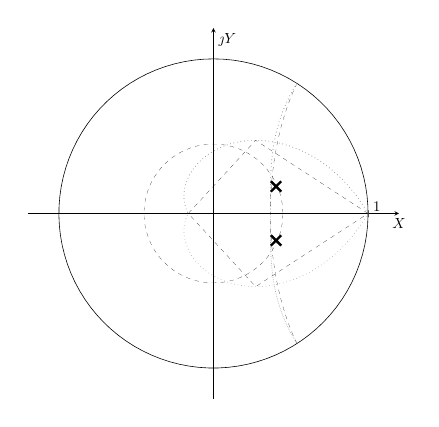
\begin{tikzpicture}[scale=0.53]

\begin{axis}[%
  axis lines=center,
  width=3.5in,
  height=3.5in,
  scale only axis,
  unbounded coords=jump,
  xmin=-1.2,
  xmax=1.2,
  ymin=-1.2,
  ymax=1.2,
  xtick={1},
  ytick=\empty,
  xticklabel style={anchor=south west, draw=none},
  xlabel={$X$},
  ylabel={$\jmath Y$},
  x label style={anchor=north}
]
\addplot [color=black!40, dotted, forget plot]
  table[row sep=crcr]{%
1	0\\
0.994975166457918	0.0086169531277774\\
0.989901329986755	0.0171473087453408\\
0.98477948302476	0.0255910797348211\\
0.979610612912339	0.0339482874654127\\
0.97439570184454	0.0422189617067992\\
0.96913572682452	0.0504031405426052\\
0.963831659617994	0.0585008702838818\\
0.958484466708655	0.0665122053826345\\
0.953095109254565	0.0744372083454012\\
0.947664543045514	0.0822759496468887\\
0.942193718461326	0.0900285076436762\\
0.936683580431134	0.0976949684879922\\
0.931135068393585	0.105275426041575\\
0.925549116258005	0.112769981789622\\
0.919926652366486	0.120178744754836\\
0.914268599456912	0.127501831411582\\
0.90857587462691	0.134739365600147\\
0.902849389298715	0.14189147844113\\
0.89709004918496	0.148958308249953\\
0.891298754255365	0.155940000451509\\
0.88547639870433	0.162836707494953\\
0.879623870919433	0.169648588768638\\
0.873742053450808	0.176375810515214\\
0.867831822981418	0.183018545746879\\
0.8618940502982	0.189576974160811\\
0.855929600264091	0.196051282054771\\
0.849939331790917	0.202441662242887\\
0.843924097813143	0.208748313971631\\
0.837884745262484	0.214971442835991\\
0.831822115043362	0.221111260695846\\
0.825737042009206	0.227167985592546\\
0.819630354939596	0.233141841665717\\
0.81350287651823	0.23903305907027\\
0.807355423311723	0.244841873893657\\
0.801188805749226	0.250568528073344\\
0.795003828102853	0.256213269314532\\
0.78880128846892	0.26177635100812\\
0.782581978749986	0.267258032148917\\
0.776346684637685	0.272658577254117\\
0.770096185596349	0.277978256282022\\
0.763831254847411	0.283217344551051\\
0.757552659354593	0.288376122659003\\
0.751261159809852	0.293454876402612\\
0.744957510620097	0.298453896697378\\
0.738642459894664	0.303373479497687\\
0.732316749433537	0.308213925717227\\
0.725981114716321	0.312975541149701\\
0.719636284891949	0.317658636389843\\
0.71328298276912	0.322263526754741\\
0.706921924807467	0.326790532205477\\
0.700553821109446	0.331239977269081\\
0.694179375412927	0.335612190960806\\
0.687799285084511	0.339907506706737\\
0.681414241113527	0.344126262266724\\
0.675024928106738	0.34826879965765\\
0.668632024283728	0.352335465077047\\
0.662236201472974	0.356326608827046\\
0.65583812510859	0.360242585238686\\
0.649438454227737	0.364083752596562\\
0.643037841468706	0.367850473063845\\
0.636636933069644	0.371543112607646\\
0.630236368867939	0.375162040924758\\
0.623836782300241	0.378707631367759\\
0.617438800403127	0.382180260871485\\
0.611043043814387	0.385580309879881\\
0.604650126774944	0.388908162273233\\
0.598260657131382	0.392164205295778\\
0.591875236339095	0.395348829483698\\
0.585494459466028	0.398462428593512\\
0.579118915197029	0.401505399530848\\
0.572749185838786	0.40447814227962\\
0.566385847325349	0.4073810598316\\
0.560029469224235	0.410214558116388\\
0.553680614743102	0.412979045931794\\
0.547339840736992	0.415674934874619\\
0.541007697716132	0.418302639271854\\
0.534684729854293	0.420862576112287\\
0.528371474997687	0.423355164978523\\
0.522068464674416	0.425780827979435\\
0.515776224104452	0.428139989683019\\
0.509495272210138	0.430433077049683\\
0.503226121627222	0.432660519365961\\
0.496969278716402	0.434822748178651\\
0.490725243575377	0.436920197229388\\
0.484494510051408	0.438953302389643\\
0.478277565754372	0.440922501596166\\
0.472074892070308	0.44282823478686\\
0.465886964175444	0.444670943837092\\
0.459714251050707	0.446451072496453\\
0.453557215496707	0.448169066325949\\
0.447416314149175	0.449825372635651\\
0.441291997494877	0.451420440422779\\
0.435184709887969	0.452954720310238\\
0.429094889566804	0.454428664485608\\
0.423022968671182	0.455842726640584\\
0.416969373260031	0.457197361910859\\
0.410934523329524	0.458493026816478\\
0.404918832831608	0.459730179202636\\
0.398922709692961	0.460909278180935\\
0.392946555834355	0.462030784071105\\
0.386990767190422	0.463095158343177\\
0.381055733729824	0.46410286356012\\
0.375141839475811	0.465054363320948\\
0.369249462527169	0.465950122204273\\
0.363378975079551	0.466790605712337\\
0.357530743447174	0.467576280215505\\
0.351705128084897	0.46830761289722\\
0.345902483610657	0.468985071699428\\
0.34012315882826	0.469609125268472\\
0.334367496750526	0.47018024290145\\
0.328635834622783	0.470698894493046\\
0.322928503946697	0.471165550482829\\
0.317245830504437	0.471580681803022\\
0.311588134383171	0.471944759826739\\
0.305955729999881	0.472258256316704\\
0.300348926126498	0.472521643374422\\
0.294768025915352	0.472735393389845\\
0.289213326924917	0.47289997899149\\
0.283685121145871	0.473015872997045\\
0.278183695027438	0.473083548364434\\
0.272709329504025	0.473103478143368\\
0.267262300022144	0.473076135427362\\
0.261842876567611	0.473001993306221\\
0.256451323693014	0.472881524819009\\
0.251087900545453	0.472715202907487\\
0.24575286089454	0.472503500370018\\
0.240446453160655	0.472246889815953\\
0.235168920443456	0.471945843620488\\
0.229920500550629	0.471600833879988\\
0.224701426026886	0.471212332367794\\
0.219511924183188	0.470780810490488\\
0.214352217126212	0.470306739244642\\
0.209222521788028	0.46979058917403\\
0.204123049956005	0.469232830327317\\
0.199054008302929	0.468633932216212\\
0.194015598417329	0.467994363774097\\
0.189008016834009	0.467314593315119\\
0.184031455064777	0.466595088493758\\
0.179086099629367	0.465836316264853\\
0.174172132086558	0.465038742844109\\
0.169289729065466	0.464202833669053\\
0.16443906229702	0.463329053360474\\
0.159620298645616	0.462417865684317\\
0.154833600140936	0.461469733514039\\
0.150079124009928	0.460485118793442\\
0.145357022708955	0.45946448249995\\
0.140667443956089	0.458408284608366\\
0.136010530763565	0.457316984055071\\
0.131386421470369	0.456191038702701\\
0.126795249774977	0.455030905305267\\
0.122237144768225	0.453837039473741\\
0.117712230966311	0.452609895642096\\
0.113220628343922	0.451349927033798\\
0.108762452367488	0.450057585628759\\
0.104337814028549	0.448733322130736\\
0.0999468198772385	0.447377585935182\\
0.0955895720558732	0.445990825097552\\
0.0912661683326492	0.444573486302051\\
0.0869767021354367	0.443126014830835\\
0.0827212625856707	0.441648854533653\\
0.0784999345323338	0.440142447797942\\
0.0743127985860244	0.438607235519351\\
0.0701599311531092	0.437043657072723\\
0.0660414044699528	0.435452150283505\\
0.0619572866372231	0.433833151399599\\
0.0579076416542657	0.432187095063656\\
0.0538925294535447	0.4305144142858\\
0.0499120059351455	0.428815540416786\\
0.045966123001336	0.42709090312159\\
0.0420549285911806	0.425340930353435\\
0.0381784667152051	0.423566048328237\\
0.0343367774901069	0.421766681499485\\
0.0305298971735083	0.419943252533545\\
0.0267578581987466	0.418096182285383\\
0.0230206892096994	0.416225889774718\\
0.0193184150956407	0.414332792162584\\
0.0156510570261221	0.412417304728323\\
0.0120186324858799	0.410479840846984\\
0.00842115530975893	0.408520811967138\\
0.00485863571765306	0.406540627589113\\
0.00133108034945763	0.404539695243628\\
-0.00216150769996924	0.402518420470845\\
-0.00561912884584125	0.400477206799821\\
-0.00904178697847668	0.39841645572837\\
-0.0124294894283334	0.396336566703324\\
-0.0157822469310498	0.394237937101194\\
-0.0191000735924938	0.39212096220923\\
-0.0223829868538259	0.389986035206885\\
-0.0256310074565762	0.387833547147654\\
-0.028844159407742	0.385663886941331\\
-0.0320224699449067	0.383477441336632\\
-0.035165969501385	0.381274594904221\\
-0.0382746916713966	0.379055730020116\\
-0.0413486731752722	0.37682122684948\\
-0.044387953824694	0.374571463330791\\
-0.0473925764879758	0.372306815160395\\
-0.0503625870553824	0.37002765577743\\
-0.053298034404496	0.367734356349131\\
-0.0561989703656271	0.365427285756506\\
-0.0590654496872782	0.363106810580375\\
-0.0618975300016593	0.360773295087786\\
-0.0646952717902602	0.358427101218792\\
-0.0674587383494818	0.356068588573591\\
-0.0701879957563293	0.353698114400028\\
-0.0728831128341696	0.351316033581455\\
-0.0755441611185572	0.348922698624945\\
-0.078171214823129	0.346518459649865\\
-0.080764350805573	0.344103664376793\\
-0.083323648533672	0.341678658116792\\
-0.0858491900514256	0.339243783761024\\
-0.0883410599452533	0.336799381770708\\
-0.0907993453102799	0.334345790167427\\
-0.0932241357167081	0.331883344523768\\
-0.0956155231762785	0.329412377954299\\
-0.0979736021088205	0.326933221106879\\
-0.100298469308897	0.324446202154309\\
-0.102590223912543	0.3219516467863\\
-0.104848967364106	0.319449878201778\\
-0.107074803383181	0.316941217101503\\
-0.109267837931654	0.314425981681024\\
-0.111428179180845	0.311904487623941\\
-0.113555937478763	0.309377048095487\\
-0.115651225317466	0.306843973736431\\
-0.117714157300535	0.304305572657284\\
-0.119744850110663	0.301762150432819\\
-0.121743422477352	0.299214010096897\\
-0.12370999514474	0.296661452137599\\
-0.125644690839534	0.294104774492655\\
-0.127547634239077	0.29154427254518\\
-0.129418951939533	0.288980239119696\\
-0.131258772424195	0.286412964478459\\
-0.133067226031924	0.283842736318072\\
-0.13484444492572	0.281269839766384\\
-0.136590563061418	0.278694557379684\\
-0.138305716156522	0.27611716914017\\
-0.139990041659173	0.273537952453705\\
-0.141643678717248	0.27095718214785\\
-0.143266768147609	0.268375130470173\\
-0.144859452405477	0.26579206708683\\
-0.146421875553965	0.263208259081419\\
-0.147954183233735	0.260623970954104\\
-0.149456522632818	0.258039464621\\
-0.150929042456566	0.255454999413824\\
-0.152371892897761	0.252870832079808\\
-0.153785225606871	0.250287216781869\\
-0.155169193662457	0.24770440509903\\
-0.156523951541726	0.245122646027102\\
-0.157849655091252	0.242542185979612\\
-0.159146461497839	0.239963268788975\\
-0.160414529259544	0.237386135707918\\
-0.161654018156862	0.234811025411143\\
-0.162865089224069	0.232238173997232\\
-0.164047904720716	0.229667814990784\\
-0.165202628103302	0.227100179344793\\
-0.166329423997092	0.224535495443257\\
-0.167428458168113	0.221973989104012\\
-0.168499897495306	0.219415883581802\\
-0.169543909942848	0.216861399571562\\
-0.170560664532644	0.214310755211935\\
-0.171550331316981	0.211764166088996\\
-0.172513081351356	0.209221845240208\\
-0.173449086667475	0.206684003158576\\
-0.174358520246424	0.204150847797023\\
-0.175241555992005	0.201622584572976\\
-0.176098368704256	0.199099416373151\\
-0.176929134053141	0.196581543558548\\
-0.177734028552409	0.194069163969646\\
-0.178513229533643	0.191562472931801\\
-0.179266915120471	0.189061663260829\\
-0.179995264202967	0.1865669252688\\
-0.180698456412218	0.184078446770007\\
-0.181376672095087	0.181596413087137\\
-0.182030092289137	0.17912100705762\\
-0.18265889869775	0.176652409040165\\
-0.183263273665422	0.17419079692148\\
-0.183843400153239	0.171736346123169\\
-0.184399461714537	0.169289229608803\\
-0.184931642470749	0.16684961789117\\
-0.185440127087425	0.164417679039694\\
-0.185925100750451	0.161993578688022\\
-0.186386749142441	0.159577480041785\\
-0.18682525841932	0.157169543886511\\
-0.18724081518709	0.154769928595712\\
-0.18763360647879	0.152378790139125\\
-0.18800381973163	0.149996282091108\\
-0.188351642764323	0.147622555639199\\
-0.1886772637546	0.145257759592815\\
-0.188980871216915	0.142902040392114\\
-0.189262653980335	0.140555542116997\\
-0.189522801166623	0.138218406496255\\
-0.189761502168506	0.135890772916862\\
-0.189978946628136	0.133572778433407\\
-0.190175324415737	0.131264557777667\\
-0.190350825608445	0.128966243368309\\
-0.190505640469335	0.126677965320734\\
-0.19063995942664	0.124399851457046\\
-0.190753973053159	0.122132027316154\\
-0.19084787204586	0.119874616163997\\
-0.190921847205665	0.117627739003896\\
-0.190976089417432	0.11539151458703\\
-0.191010789630132	0.113166059423026\\
-0.191026138837202	0.110951487790669\\
-0.191022328057108	0.108747911748734\\
-0.190999548314082	0.106555441146921\\
-0.190957990619064	0.104374183636905\\
-0.190897845950822	0.1022042446835\\
-0.190819305237275	0.100045727575919\\
-0.190722559336998	0.0978987334391491\\
-0.190607799020923	0.0957633612454201\\
-0.190475214954231	0.0936397078257795\\
-0.190324997678427	0.0915278678817618\\
-0.190157337593618	0.0894279339971549\\
-0.189972424940972	0.0873399966498598\\
-0.18977044978537	0.0852641442238417\\
-0.18955160199825	0.083200463021171\\
-0.189316071240637	0.0811490372741514\\
-0.189064046946367	0.0791099491575331\\
-0.1887957183055	0.0770832788008092\\
-0.18851127424792	0.0750691043005936\\
-0.18821090342712	0.073067501733078\\
-0.187894794204192	0.0710785451665654\\
-0.187563134631983	0.0691023066740791\\
-0.187216112439458	0.0671388563460452\\
-0.186853915016241	0.065188262303045\\
-0.186476729397344	0.0632505907086381\\
-0.186084742248091	0.0613259057822507\\
-0.185678139849218	0.0594142698121313\\
-0.185257108082164	0.0575157431683673\\
-0.184821832414555	0.0556303843159656\\
-0.18437249788586	0.0537582498279896\\
-0.183909289093245	0.0518993943987567\\
-0.183432390177603	0.0500538708570886\\
-0.182941984809774	0.0482217301796184\\
-0.182438256176944	0.0464030215041461\\
-0.181921386969236	0.044597792143048\\
-0.18139155936647	0.0428060875967306\\
-0.180848955025119	0.041027951567134\\
-0.180293755065441	0.0392634259712775\\
-0.179726140058791	0.0375125509548501\\
-0.179146290015116	0.0357753649058401\\
-0.178554384370631	0.0340519044682056\\
-0.177950601975674	0.032342204555581\\
-0.177335121082737	0.0306462983650213\\
-0.176708119334683	0.0289642173907774\\
-0.176069773753131	0.0272959914381074\\
-0.175420260727028	0.0256416486371157\\
-0.174759756001391	0.0240012154566223\\
-0.174088434666228	0.0223747167180594\\
-0.173406471145636	0.0207621756093928\\
-0.172714039187066	0.0191636136990689\\
-0.172011311850774	0.0175790509499823\\
-0.171298461499436	0.0160085057334652\\
-0.170575659787937	0.0144519948432961\\
-0.16984307765334	0.0129095335097251\\
-0.169100885305011	0.0113811354135165\\
-0.168349252214934	0.00986681270000477\\
-0.167588347108177	0.00836657599316387\\
-0.166818337953539	0.00688043440968819\\
-0.166039391954362	0.00540839557308299\\
-0.165251675539513	0.00395046562776311\\
-0.164455354354524	0.00250664925315921\\
-0.163650593252911	0.00107694967782874\\
};

\addplot [color=black!40, dotted, forget plot, each nth point=10]
  table[row sep=crcr]{%
0.54030230586814	0.841470984807897\\
0.539762693938401	0.840629664537062\\
0.539224460721023	0.83978864621053\\
0.53868760316101	0.838947930597949\\
0.538152118209836	0.838107518462474\\
0.537618002825427	0.837267410560788\\
0.537085253972145	0.836427607643129\\
0.53655386862078	0.835588110453312\\
0.536023843748535	0.83474891972876\\
0.535495176339009	0.833910036200521\\
0.534967863382191	0.833071460593297\\
0.534441901874438	0.832233193625467\\
0.533917288818469	0.831395236009111\\
0.533394021223349	0.830557588450033\\
0.532872096104475	0.829720251647789\\
0.532351510483565	0.828883226295704\\
0.531832261388641	0.828046513080903\\
0.531314345854023	0.827210112684328\\
0.530797760920307	0.826374025780767\\
0.53028250363436	0.825538253038873\\
0.529768571049302	0.82470279512119\\
0.529255960224495	0.823867652684175\\
0.528744668225529	0.823032826378221\\
0.52823469212421	0.822198316847678\\
0.527726028998549	0.821364124730882\\
0.527218675932742	0.820530250660169\\
0.526712630017168	0.819696695261905\\
0.526207888348365	0.818863459156502\\
0.525704448029027	0.818030542958447\\
0.525202306167984	0.817197947276319\\
0.524701459880193	0.816365672712812\\
0.524201906286724	0.815533719864761\\
0.523703642514747	0.814702089323156\\
0.523206665697522	0.813870781673172\\
0.522710972974383	0.813039797494186\\
0.522216561490726	0.8122091373598\\
0.521723428397999	0.811378801837861\\
0.521231570853687	0.810548791490484\\
0.5207409860213	0.809719106874073\\
0.520251671070359	0.808889748539341\\
0.519763623176388	0.808060717031331\\
0.519276839520897	0.80723201288944\\
0.518791317291371	0.806403636647435\\
0.518307053681259	0.805575588833477\\
0.51782404588996	0.80474786997014\\
0.517342291122811	0.803920480574434\\
0.516861786591075	0.803093421157821\\
0.516382529511928	0.802266692226238\\
0.515904517108448	0.80144029428012\\
0.515427746609602	0.800614227814413\\
0.514952215250233	0.799788493318601\\
0.514477920271049	0.79896309127672\\
0.514004858918611	0.798138022167384\\
0.51353302844532	0.797313286463798\\
0.513062426109404	0.796488884633783\\
0.512593049174908	0.795664817139792\\
0.512124894911682	0.794841084438931\\
0.511657960595367	0.794017686982978\\
0.511192243507383	0.793194625218402\\
0.510727740934919	0.792371899586382\\
0.510264450170919	0.791549510522827\\
0.509802368514074	0.790727458458392\\
0.509341493268803	0.7899057438185\\
0.508881821745247	0.789084367023359\\
0.508423351259256	0.788263328487982\\
0.507966079132375	0.787442628622202\\
0.507510002691835	0.786622267830696\\
0.507055119270539	0.785802246512997\\
0.506601426207052	0.784982565063518\\
0.506148920845586	0.784163223871566\\
0.505697600535993	0.78334422332136\\
0.505247462633751	0.782525563792053\\
0.504798504499949	0.781707245657746\\
0.504350723501283	0.780889269287506\\
0.503904117010036	0.780071635045386\\
0.503458682404072	0.779254343290439\\
0.503014417066823	0.77843739437674\\
0.502571318387277	0.777620788653398\\
0.502129383759965	0.776804526464577\\
0.501688610584954	0.775988608149514\\
0.501248996267831	0.775173034042531\\
0.500810538219691	0.774357804473059\\
0.500373233857132	0.773542919765647\\
0.499937080602236	0.772728380239986\\
0.499502075882562	0.771914186210922\\
0.499068217131134	0.771100337988471\\
0.498635501786428	0.770286835877842\\
0.498203927292362	0.769473680179445\\
0.497773491098285	0.768660871188913\\
0.497344190658966	0.767848409197119\\
0.49691602343458	0.767036294490186\\
0.496488986890701	0.766224527349511\\
0.496063078498286	0.765413108051773\\
0.495638295733668	0.764602036868957\\
0.495214636078543	0.763791314068363\\
0.49479209701996	0.762980939912625\\
0.494370676050306	0.762170914659728\\
0.493950370667301	0.761361238563018\\
0.493531178373981	0.760551911871226\\
0.493113096678692	0.759742934828473\\
0.492696123095076	0.758934307674296\\
0.49228025514206	0.758126030643656\\
0.491865490343845	0.757318103966953\\
0.491451826229899	0.756510527870047\\
0.491039260334939	0.755703302574268\\
0.490627790198926	0.754896428296429\\
0.490217413367051	0.754089905248849\\
0.489808127389725	0.753283733639359\\
0.48939992982257	0.75247791367132\\
0.488992818226405	0.751672445543641\\
0.488586790167236	0.750867329450786\\
0.488181843216247	0.750062565582796\\
0.487777974949788	0.749258154125298\\
0.487375182949364	0.748454095259521\\
0.486973464801624	0.747650389162311\\
0.486572818098353	0.746847036006143\\
0.486173240436456	0.746044035959138\\
0.485774729417954	0.745241389185073\\
0.485377282649968	0.744439095843398\\
0.484980897744711	0.743637156089248\\
0.484585572319477	0.742835570073457\\
0.484191303996629	0.742034337942574\\
0.483798090403591	0.74123345983887\\
0.483405929172836	0.740432935900359\\
0.483014817941875	0.739632766260805\\
0.482624754353249	0.738832951049743\\
0.482235736054514	0.738033490392481\\
0.481847760698234	0.737234384410123\\
0.481460825941973	0.736435633219578\\
0.481074929448277	0.735637236933574\\
0.480690068884672	0.734839195660667\\
0.480306241923647	0.734041509505259\\
0.479923446242647	0.733244178567608\\
0.479541679524064	0.732447202943843\\
0.479160939455223	0.73165058272597\\
0.478781223728375	0.730854318001894\\
0.478402530040683	0.730058408855422\\
0.478024856094217	0.729262855366284\\
0.477648199595939	0.728467657610137\\
0.477272558257696	0.727672815658583\\
0.476897929796208	0.726878329579179\\
0.476524311933058	0.726084199435447\\
0.476151702394684	0.725290425286892\\
0.475780098912366	0.724497007189005\\
0.475409499222216	0.723703945193283\\
0.475039901065173	0.722911239347235\\
0.474671302186985	0.722118889694397\\
0.474303700338206	0.721326896274341\\
0.47393709327418	0.720535259122689\\
0.473571478755038	0.719743978271122\\
0.473206854545681	0.718953053747392\\
0.472843218415775	0.718162485575335\\
0.472480568139739	0.71737227377488\\
0.472118901496735	0.716582418362059\\
0.471758216270658	0.715792919349022\\
0.47139851025013	0.715003776744045\\
0.471039781228482	0.71421499055154\\
0.470682027003753	0.713426560772069\\
0.470325245378674	0.712638487402353\\
0.469969434160663	0.71185077043528\\
0.46961459116181	0.71106340985992\\
0.469260714198871	0.710276405661534\\
0.468907801093259	0.709489757821582\\
0.46855584967103	0.708703466317736\\
0.468204857762879	0.70791753112389\\
0.467854823204124	0.707131952210168\\
0.467505743834703	0.706346729542938\\
0.467157617499157	0.705561863084818\\
0.46681044204663	0.704777352794687\\
0.46646421533085	0.703993198627698\\
0.466118935210123	0.703209400535282\\
0.465774599547328	0.702425958465164\\
0.465431206209898	0.701642872361368\\
0.46508875306982	0.700860142164228\\
0.46474723800362	0.700077767810399\\
0.464406658892354	0.699295749232865\\
0.464067013621601	0.698514086360948\\
0.463728300081451	0.697732779120317\\
0.463390516166498	0.696951827433\\
0.463053659775829	0.69617123121739\\
0.462717728813013	0.695390990388255\\
0.462382721186096	0.694611104856748\\
0.462048634807588	0.693831574530415\\
0.461715467594456	0.693052399313204\\
0.461383217468113	0.692273579105474\\
0.46105188235441	0.691495113804002\\
0.460721460183626	0.690717003301996\\
0.460391948890459	0.689939247489099\\
0.460063346414016	0.6891618462514\\
0.459735650697807	0.68838479947144\\
0.459408859689731	0.687608107028223\\
0.459082971342071	0.686831768797225\\
0.458757983611482	0.686055784650399\\
0.458433894458983	0.685280154456184\\
0.45811070184995	0.684504878079514\\
0.457788403754102	0.683729955381828\\
0.457466998145497	0.682955386221072\\
0.457146483002521	0.682181170451714\\
0.456826856307877	0.681407307924745\\
0.45650811604858	0.680633798487693\\
0.456190260215944	0.679860641984627\\
0.455873286805575	0.679087838256163\\
0.455557193817364	0.678315387139476\\
0.455241979255474	0.677543288468305\\
0.454927641128334	0.676771542072959\\
0.454614177448629	0.676000147780328\\
0.454301586233291	0.675229105413887\\
0.453989865503491	0.674458414793703\\
0.45367901328463	0.673688075736445\\
0.453369027606329	0.672918088055388\\
0.453059906502422	0.672148451560422\\
0.452751648010945	0.671379166058059\\
0.452444250174131	0.670610231351436\\
0.452137711038396	0.669841647240328\\
0.451832028654334	0.669073413521148\\
0.451527201076709	0.668305529986959\\
0.451223226364442	0.667537996427477\\
0.450920102580607	0.666770812629081\\
0.45061782779242	0.666003978374815\\
0.45031640007123	0.665237493444396\\
0.450015817492511	0.664471357614223\\
0.449716078135855	0.663705570657378\\
0.449417180084962	0.662940132343639\\
0.449119121427628	0.662175042439477\\
0.448821900255744	0.66141030070807\\
0.448525514665281	0.660645906909305\\
0.448229962756284	0.659881860799785\\
0.447935242632865	0.659118162132834\\
0.44764135240319	0.658354810658502\\
0.447348290179475	0.657591806123574\\
0.447056054077976	0.65682914827157\\
0.44676464221898	0.656066836842755\\
0.446474052726798	0.655304871574145\\
0.446184283729755	0.654543252199506\\
0.445895333360182	0.653781978449367\\
0.445607199754407	0.65302105005102\\
0.445319881052752	0.652260466728527\\
0.445033375399515	0.651500228202724\\
0.444747680942969	0.650740334191229\\
0.444462795835354	0.649980784408442\\
0.444178718232864	0.649221578565555\\
0.443895446295641	0.648462716370551\\
0.443612978187767	0.647704197528215\\
0.443331312077259	0.646946021740133\\
0.443050446136053	0.6461881887047\\
0.442770378540003	0.645430698117124\\
0.44249110746887	0.644673549669429\\
0.442212631106314	0.643916743050459\\
0.441934947639884	0.643160277945886\\
0.441658055261015	0.64240415403821\\
0.441381952165015	0.641648371006764\\
0.441106636551058	0.64089292852772\\
0.440832106622177	0.640137826274091\\
0.440558360585258	0.639383063915734\\
0.440285396651025	0.638628641119359\\
0.44001321303404	0.637874557548525\\
0.43974180795269	0.63712081286365\\
0.439471179629181	0.636367406722011\\
0.439201326289529	0.63561433877775\\
0.438932246163553	0.634861608681876\\
0.438663937484865	0.634109216082268\\
0.438396398490867	0.633357160623679\\
0.438129627422738	0.632605441947739\\
0.437863622525426	0.631854059692959\\
0.437598382047645	0.631103013494734\\
0.437333904241863	0.630352302985342\\
0.437070187364295	0.629601927793954\\
0.436807229674897	0.628851887546632\\
0.436545029437354	0.628102181866332\\
0.436283584919079	0.627352810372908\\
0.436022894391196	0.626603772683115\\
0.435762956128542	0.625855068410611\\
0.435503768409653	0.625106697165959\\
0.435245329516757	0.624358658556628\\
0.434987637735768	0.623610952186999\\
0.434730691356278	0.622863577658366\\
0.434474488671548	0.622116534568935\\
0.434219027978502	0.621369822513831\\
0.433964307577718	0.620623441085097\\
0.433710325773422	0.619877389871695\\
0.433457080873477	0.619131668459512\\
0.433204571189379	0.618386276431358\\
0.43295279503625	0.617641213366968\\
0.432701750732826	0.616896478843007\\
0.432451436601452	0.616152072433068\\
0.432201850968076	0.615407993707675\\
0.431952992162239	0.614664242234284\\
0.431704858517069	0.613920817577285\\
0.431457448369273	0.613177719298002\\
0.431210760059128	0.612434946954695\\
0.430964791930477	0.611692500102562\\
0.430719542330718	0.610950378293739\\
0.4304750096108	0.610208581077301\\
0.430231192125212	0.609467107999262\\
0.429988088231978	0.608725958602578\\
0.429745696292648	0.607985132427146\\
0.429504014672294	0.607244629009805\\
0.429263041739498	0.606504447884337\\
0.429022775866347	0.605764588581468\\
0.428783215428427	0.605025050628865\\
0.428544358804814	0.604285833551141\\
0.428306204378065	0.603546936869854\\
0.428068750534215	0.602808360103502\\
0.427831995662766	0.602070102767534\\
0.427595938156682	0.601332164374336\\
0.427360576412381	0.600594544433245\\
0.427125908829728	0.599857242450537\\
0.426891933812026	0.599120257929434\\
0.426658649766011	0.598383590370103\\
0.426426055101846	0.59764723926965\\
0.426194148233109	0.596911204122128\\
0.425962927576792	0.596175484418529\\
0.425732391553288	0.595440079646789\\
0.425502538586388	0.594704989291781\\
0.425273367103272	0.59397021283532\\
0.425044875534504	0.593235749756162\\
0.424817062314021	0.592501599529995\\
0.42458992587913	0.59176776162945\\
0.424363464670499	0.59103423552409\\
0.424137677132149	0.590301020680412\\
0.42391256171145	0.589568116561847\\
0.423688116859112	0.58883552262876\\
0.423464341029178	0.58810323833844\\
0.423241232679015	0.587371263145111\\
0.423018790269314	0.586639596499918\\
0.422797012264074	0.585908237850935\\
0.422575897130603	0.585177186643157\\
0.422355443339504	0.584446442318501\\
0.422135649364675	0.583716004315801\\
0.421916513683297	0.582985872070811\\
0.421698034775829	0.582256045016197\\
0.421480211126001	0.581526522581538\\
0.421263041220808	0.580797304193323\\
0.421046523550503	0.58006838927495\\
0.420830656608586	0.579339777246718\\
0.420615438891806	0.578611467525831\\
0.420400868900144	0.577883459526392\\
0.420186945136815	0.5771557526594\\
0.419973666108256	0.576428346332746\\
0.41976103032412	0.575701239951214\\
0.419549036297272	0.574974432916473\\
0.419337682543778	0.574247924627077\\
0.419126967582901	0.57352171447846\\
0.418916889937096	0.572795801862935\\
0.418707448131999	0.572070186169684\\
0.418498640696424	0.571344866784765\\
0.418290466162353	0.570619843091098\\
0.418082923064934	0.569895114468466\\
0.417876009942469	0.569170680293511\\
0.417669725336412	0.56844653993973\\
0.41746406779136	0.567722692777469\\
0.417259035855045	0.566999138173921\\
0.417054628078333	0.56627587549312\\
0.416850843015211	0.565552904095938\\
0.416647679222784	0.564830223340079\\
0.416445135261268	0.564107832580074\\
0.416243209693983	0.56338573116728\\
0.416041901087346	0.562663918449871\\
0.415841208010867	0.561942393772834\\
0.415641129037138	0.561221156477965\\
0.415441662741833	0.560500205903863\\
0.415242807703694	0.559779541385926\\
0.415044562504532	0.559059162256343\\
0.414846925729215	0.558339067844093\\
0.414649895965663	0.557619257474932\\
0.414453471804843	0.556899730471397\\
0.414257651840763	0.556180486152791\\
0.414062434670464	0.555461523835183\\
0.413867818894012	0.554742842831401\\
0.413673803114496	0.554024442451023\\
0.413480385938019	0.553306322000374\\
0.413287565973692	0.552588480782517\\
0.413095341833629	0.55187091809725\\
0.412903712132937	0.551153633241096\\
0.412712675489714	0.550436625507298\\
0.412522230525041	0.549719894185811\\
0.412332375862976	0.549003438563298\\
0.412143110130546	0.548287257923117\\
0.411954431957746	0.547571351545322\\
0.411766339977524	0.546855718706648\\
0.411578832825784	0.546140358680509\\
0.411391909141374	0.545425270736987\\
0.411205567566082	0.544710454142827\\
0.411019806744629	0.543995908161427\\
0.410834625324664	0.543281632052833\\
0.410650021956757	0.542567625073726\\
0.410465995294393	0.541853886477419\\
0.410282543993964	0.541140415513847\\
0.410099666714769	0.540427211429558\\
0.409917362119	0.539714273467703\\
0.409735628871742	0.539001600868033\\
0.409554465640962	0.538289192866882\\
0.409373871097508	0.537577048697166\\
0.409193843915101	0.536865167588369\\
0.409014382770325	0.536153548766536\\
0.408835486342629	0.535442191454261\\
0.408657153314313	0.534731094870683\\
0.408479382370527	0.534020258231471\\
0.408302172199265	0.533309680748816\\
0.408125521491354	0.532599361631423\\
0.407949428940455	0.531889300084499\\
0.407773893243052	0.531179495309743\\
0.407598913098449	0.530469946505337\\
0.407424487208762	0.529760652865935\\
0.407250614278914	0.529051613582652\\
0.40707729301663	0.528342827843053\\
0.406904522132429	0.527634294831145\\
0.406732300339621	0.526926013727362\\
0.406560626354297	0.526217983708558\\
0.40638949889533	0.525510203947991\\
0.40621891668436	0.524802673615316\\
0.406048878445796	0.524095391876573\\
0.405879382906807	0.523388357894171\\
0.405710428797317	0.522681570826882\\
0.405542014849996	0.521975029829825\\
0.40537413980026	0.521268734054456\\
0.405206802386261	0.520562682648553\\
0.405040001348882	0.519856874756209\\
0.404873735431734	0.519151309517812\\
0.404708003381144	0.518445986070039\\
0.404542803946157	0.517740903545838\\
0.404378135878525	0.51703606107442\\
0.404213997932703	0.51633145778124\\
0.404050388865844	0.515627092787988\\
0.403887307437792	0.514922965212575\\
0.403724752411077	0.514219074169115\\
0.403562722550909	0.513515418767917\\
0.403401216625174	0.512811998115469\\
0.403240233404426	0.51210881131442\\
0.403079771661883	0.511405857463572\\
0.40291983017342	0.510703135657861\\
0.402760407717566	0.510000644988341\\
0.402601503075495	0.509298384542175\\
0.402443115031024	0.508596353402615\\
0.402285242370605	0.507894550648989\\
0.402127883883318	0.507192975356682\\
0.401971038360872	0.506491626597125\\
0.401814704597591	0.505790503437778\\
0.401658881390416	0.505089604942113\\
0.401503567538893	0.504388930169596\\
0.401348761845173	0.503688478175676\\
0.401194463114003	0.502988248011761\\
0.401040670152722	0.50228823872521\\
0.400887381771257	0.501588449359308\\
0.400734596782113	0.500888878953255\\
0.400582314000372	0.500189526542143\\
0.400430532243686	0.499490391156944\\
0.400279250332273	0.49879147182449\\
0.400128467088907	0.498092767567452\\
0.399978181338919	0.497394277404329\\
0.399828391910187	0.496696000349422\\
0.399679097633134	0.495997935412819\\
0.399530297340718	0.495300081600379\\
0.399381989868431	0.494602437913709\\
0.399234174054294	0.493905003350143\\
0.399086848738846	0.49320777690273\\
0.398940012765147	0.492510757560208\\
0.398793664978765	0.491813944306987\\
0.398647804227776	0.491117336123128\\
0.398502429362755	0.490420931984323\\
0.398357539236775	0.489724730861874\\
0.398213132705398	0.489028731722674\\
0.39806920862667	0.488332933529185\\
0.397925765861118	0.487637335239415\\
0.397782803271744	0.486941935806902\\
0.39764031972402	0.486246734180684\\
0.39749831408588	0.485551729305286\\
0.397356785227718	0.484856920120692\\
0.397215732022384	0.484162305562325\\
0.397075153345175	0.483467884561025\\
0.396935048073831	0.482773656043023\\
0.396795415088531	0.482079618929922\\
0.396656253271888	0.481385772138671\\
0.396517561508943	0.480692114581542\\
0.396379338687161	0.479998645166107\\
0.396241583696423	0.479305362795214\\
0.396104295429024	0.478612266366961\\
0.395967472779668	0.477919354774671\\
0.395831114645461	0.477226626906872\\
0.395695219925906	0.476534081647265\\
0.395559787522899	0.475841717874705\\
0.395424816340726	0.475149534463171\\
0.395290305286053	0.47445753028174\\
0.395156253267925	0.473765704194565\\
0.395022659197758	0.473074055060844\\
0.39488952198934	0.472382581734794\\
0.394756840558816	0.471691283065628\\
0.394624613824694	0.47100015789752\\
0.394492840707832	0.470309205069586\\
0.394361520131436	0.46961842341585\\
0.394230651021055	0.468927811765217\\
0.394100232304577	0.468237368941446\\
0.393970262912223	0.467547093763121\\
0.393840741776541	0.466856985043618\\
0.393711667832403	0.466167041591083\\
0.393583040017001	0.465477262208394\\
0.393454857269837	0.464787645693136\\
0.393327118532725	0.464098190837569\\
0.393199822749781	0.4634088964286\\
0.393072968867421	0.462719761247745\\
0.392946555834355	0.462030784071105\\
0.392820582601581	0.461341963669332\\
0.392695048122384	0.460653298807593\\
0.392569951352326	0.459964788245545\\
0.392445291249246	0.459276430737294\\
0.392321066773252	0.458588225031369\\
0.392197276886717	0.457900169870683\\
0.392073920554277	0.457212263992505\\
0.39195099674282	0.456524506128419\\
0.391828504421489	0.455836895004296\\
0.391706442561671	0.455149429340254\\
0.391584810136995	0.454462107850625\\
0.391463606123327	0.453774929243921\\
0.391342829498766	0.453087892222794\\
0.391222479243636	0.452400995484003\\
0.391102554340488	0.451714237718375\\
0.390983053774088	0.451027617610771\\
0.390863976531415	0.450341133840043\\
0.39074532160166	0.449654785079001\\
0.390627087976215	0.448968569994374\\
0.390509274648673	0.448282487246767\\
0.390391880614822	0.447596535490627\\
0.39027490487264	0.4469107133742\\
0.39015834642229	0.446225019539494\\
0.390042204266118	0.445539452622235\\
0.389926477408644	0.444854011251828\\
0.389811164856562	0.444168694051316\\
0.389696265618732	0.443483499637336\\
0.389581778706177	0.442798426620081\\
0.389467703132079	0.442113473603252\\
0.389354037911772	0.44142863918402\\
0.389240782062742	0.440743921952978\\
0.389127934604617	0.4400593204941\\
0.389015494559166	0.439374833384694\\
0.388903460950293	0.438690459195361\\
0.388791832804034	0.438006196489943\\
0.388680609148552	0.437322043825484\\
0.38856978901413	0.436637999752179\\
0.388459371433172	0.435954062813327\\
0.388349355440191	0.435270231545288\\
0.388239740071813	0.434586504477429\\
0.388130524366765	0.433902880132079\\
0.388021707365875	0.433219357024479\\
0.387913288112068	0.432535933662733\\
0.387805265650358	0.431852608547757\\
0.387697639027846	0.43116938017323\\
0.387590407293716	0.43048624702554\\
0.387483569499229	0.429803207583734\\
0.38737712469772	0.429120260319467\\
0.387271071944593	0.428437403696945\\
0.387165410297317	0.427754636172876\\
0.387060138815421	0.427071956196414\\
0.38695525656049	0.426389362209102\\
0.386850762596162	0.425706852644822\\
0.38674665598812	0.425024425929735\\
0.386642935804091	0.424342080482224\\
0.386539601113843	0.423659814712842\\
0.386436650989175	0.422977627024248\\
0.38633408450392	0.422295515811153\\
0.386231900733932	0.421613479460259\\
0.386130098757092	0.420931516350199\\
0.386028677653294	0.42024962485148\\
0.385927636504448	0.419567803326417\\
0.385826974394472	0.418886050129075\\
0.385726690409287	0.418204363605205\\
0.385626783636818	0.417522742092183\\
0.385527253166984	0.416841183918943\\
0.385428098091694	0.416159687405916\\
0.385329317504849	0.415478250864961\\
0.385230910502332	0.414796872599304\\
0.385132876182003	0.414115550903467\\
0.385035213643701	0.413434284063202\\
0.384937921989234	0.412753070355424\\
0.384841000322377	0.412071908048142\\
0.384744447748868	0.411390795400386\\
0.384648263376404	0.410709730662142\\
0.384552446314637	0.410028712074277\\
0.384456995675168	0.409347737868467\\
0.384361910571546	0.408666806267126\\
0.384267190119259	0.407985915483331\\
0.384172833435737	0.407305063720748\\
0.384078839640342	0.406624249173555\\
0.383985207854366	0.405943470026369\\
0.383891937201027	0.405262724454166\\
0.383799026805465	0.404582010622205\\
0.383706475794738	0.403901326685946\\
0.383614283297815	0.403220670790976\\
0.38352244844558	0.40254004107292\\
0.383430970370817	0.401859435657368\\
0.383339848208215	0.401178852659787\\
0.38324908109436	0.400498290185438\\
0.383158668167731	0.399817746329295\\
0.383068608568697	0.399137219175953\\
0.382978901439512	0.39845670679955\\
0.382889545924312	0.397776207263671\\
0.382800541169111	0.397095718621266\\
0.382711886321796	0.396415238914558\\
0.382623580532124	0.39573476617495\\
0.382535622951719	0.395054298422939\\
0.382448012734064	0.394373833668017\\
0.382360749034503	0.393693369908582\\
0.382273831010232	0.393012905131842\\
0.382187257820298	0.392332437313717\\
0.382101028625594	0.391651964418743\\
0.382015142588854	0.390971484399974\\
0.381929598874653	0.390290995198883\\
0.381844396649398	0.38961049474526\\
0.381759535081328	0.388929980957112\\
0.381675013340508	0.388249451740556\\
0.381590830598827	0.38756890498972\\
0.381506986029992	0.386888338586634\\
0.381423478809526	0.386207750401122\\
0.381340308114762	0.3855271382907\\
0.381257473124843	0.384846500100458\\
0.381174973020713	0.384165833662956\\
0.381092806985117	0.383485136798108\\
0.381010974202598	0.382804407313071\\
0.380929473859488	0.382123643002129\\
0.38084830514391	0.381442841646577\\
0.380767467245771	0.380762001014603\\
0.380686959356758	0.380081118861167\\
0.380606780670337	0.379400192927887\\
0.380526930381746	0.378719220942907\\
0.380447407687995	0.378038200620784\\
0.380368211787857	0.377357129662353\\
0.380289341881869	0.376676005754608\\
0.380210797172326	0.375994826570569\\
0.380132576863278	0.375313589769156\\
0.380054680160527	0.374632292995054\\
0.37997710627162	0.373950933878582\\
0.379899854405851	0.373269510035555\\
0.379822923774251	0.372588019067155\\
0.379746313589589	0.371906458559785\\
0.379670023066367	0.371224826084931\\
0.379594051420814	0.370543119199023\\
0.379518397870887	0.369861335443291\\
0.379443061636263	0.369179472343616\\
0.379368041938338	0.368497527410386\\
0.379293338000221	0.367815498138347\\
0.379218949046733	0.367133382006451\\
0.379144874304403	0.366451176477703\\
0.379071113001461	0.365768878999008\\
0.37899766436784	0.36508648700101\\
0.378924527635168	0.364403997897939\\
0.378851702036765	0.363721409087443\\
0.378779186807642	0.363038717950432\\
0.378706981184494	0.362355921850909\\
0.378635084405699	0.361673018135801\\
0.378563495711313	0.360990004134794\\
0.378492214343068	0.360306877160158\\
0.378421239544366	0.359623634506574\\
0.378350570560279	0.358940273450957\\
0.378280206637541	0.35825679125228\\
0.378210147024547	0.357573185151387\\
0.378140390971353	0.356889452370817\\
0.378070937729664	0.356205590114612\\
0.378001786552838	0.355521595568135\\
0.37793293669588	0.35483746589787\\
0.377864387415437	0.354153198251239\\
0.377796137969796	0.353468789756396\\
0.377728187618882	0.352784237522037\\
0.377660535624252	0.352099538637192\\
0.377593181249092	0.351414690171024\\
0.377526123758214	0.350729689172624\\
0.377459362418054	0.350044532670794\\
0.377392896496666	0.349359217673844\\
0.377326725263721	0.348673741169368\\
0.377260847990499	0.347988100124031\\
0.377195263949893	0.347302291483345\\
0.377129972416399	0.346616312171444\\
0.377064972666117	0.345930159090859\\
0.377000263976743	0.345243829122282\\
0.376935845627572	0.344557319124338\\
0.376871716899487	0.343870625933344\\
0.376807877074962	0.343183746363069\\
0.376744325438057	0.342496677204488\\
0.376681061274411	0.341809415225537\\
0.376618083871243	0.341121957170863\\
0.376555392517349	0.340434299761564\\
0.376492986503093	0.339746439694935\\
0.376430865120411	0.339058373644207\\
0.376369027662802	0.338370098258277\\
0.376307473425328	0.337681610161441\\
0.37624620170461	0.33699290595312\\
0.376185211798823	0.336303982207584\\
0.376124503007693	0.335614835473666\\
0.376064074632498	0.334925462274484\\
0.376003925976059	0.334235859107143\\
0.375944056342739	0.333546022442447\\
0.375884465038442	0.332855948724598\\
0.375825151370604	0.332165634370895\\
0.375766114648197	0.331475075771423\\
0.375707354181721	0.330784269288746\\
0.3756488692832	0.33009321125759\\
0.375590659266182	0.329401897984517\\
0.375532723445736	0.328710325747605\\
0.375475061138444	0.328018490796116\\
0.375417671662403	0.327326389350157\\
0.375360554337219	0.326634017600341\\
0.375303708484006	0.325941371707444\\
0.37524713342538	0.325248447802048\\
0.375190828485456	0.32455524198419\\
0.375134792989849	0.323861750322997\\
0.375079026265665	0.323167968856317\\
0.375023527641503	0.32247389359035\\
0.374968296447448	0.321779520499264\\
0.374913332015069	0.321084845524814\\
0.374858633677417	0.32038986457595\\
0.374804200769022	0.319694573528419\\
0.374750032625887	0.318998968224362\\
0.374696128585488	0.318303044471906\\
0.374642487986769	0.317606798044745\\
0.37458911017014	0.316910224681722\\
0.374535994477473	0.316213320086395\\
0.374483140252101	0.315516079926602\\
0.37443054683881	0.314818499834022\\
0.374378213583842	0.314120575403719\\
0.374326139834889	0.313422302193687\\
0.374274324941088	0.312723675724387\\
0.374222768253021	0.312024691478272\\
0.374171469122712	0.311325344899309\\
0.37412042690362	0.310625631392488\\
0.374069640950642	0.309925546323332\\
0.374019110620105	0.309225085017387\\
0.373968835269765	0.308524242759712\\
0.373918814258803	0.307823014794359\\
0.373869046947824	0.307121396323845\\
0.37381953269885	0.306419382508609\\
0.373770270875324	0.305716968466471\\
0.373721260842097	0.305014149272069\\
0.373672501965436	0.3043109199563\\
0.373623993613012	0.303607275505741\\
0.373575735153902	0.302903210862063\\
0.373527725958584	0.30219872092144\\
0.373479965398935	0.301493800533939\\
0.373432452848228	0.300788444502909\\
0.373385187681128	0.300082647584354\\
0.37333816927369	0.299376404486292\\
0.373291397003357	0.298669709868113\\
0.373244870248953	0.297962558339916\\
0.373198588390686	0.297254944461841\\
0.37315255081014	0.296546862743382\\
0.373106756890275	0.295838307642699\\
0.373061206015423	0.295129273565906\\
0.373015897571285	0.294419754866355\\
0.372970830944928	0.2937097458439\\
0.372926005524784	0.292999240744158\\
0.372881420700642	0.292288233757746\\
0.372837075863654	0.291576719019509\\
0.372792970406321	0.290864690607737\\
0.3727491037225	0.290152142543361\\
0.372705475207395	0.28943906878914\\
0.372662084257558	0.288725463248833\\
0.372618930270881	0.28801131976635\\
0.3725760126466	0.287296632124895\\
0.372533330785286	0.286581394046088\\
0.372490884088846	0.28586559918907\\
0.372448671960518	0.285149241149599\\
0.372406693804871	0.284432313459118\\
0.372364949027797	0.283714809583816\\
0.372323437036515	0.28299672292366\\
0.372282157239562	0.282278046811424\\
0.372241109046793	0.28155877451168\\
0.37220029186938	0.280838899219789\\
0.372159705119805	0.280118414060861\\
0.372119348211861	0.279397312088694\\
0.372079220560646	0.278675586284701\\
0.372039321582563	0.277953229556813\\
0.371999650695315	0.277230234738351\\
0.371960207317906	0.276506594586892\\
0.371920990870632	0.275782301783101\\
0.371882000775084	0.275057348929544\\
0.371843236454142	0.274331728549476\\
0.371804697331975	0.273605433085609\\
0.371766382834034	0.272878454898846\\
0.371728292387053	0.272150786267004\\
0.371690425419047	0.271422419383494\\
0.371652781359303	0.270693346355991\\
0.371615359638387	0.269963559205061\\
0.371578159688132	0.269233049862775\\
0.37154118094164	0.268501810171284\\
0.37150442283328	0.267769831881368\\
0.371467884798682	0.267037106650954\\
0.371431566274738	0.266303626043605\\
0.371395466699595	0.265569381526977\\
0.371359585512659	0.264834364471242\\
0.371323922154583	0.264098566147477\\
0.371288476067274	0.263361977726022\\
0.371253246693882	0.2626245902748\\
0.371218233478804	0.261886394757605\\
0.371183435867678	0.261147382032347\\
0.37114885330738	0.260407542849263\\
0.371114485246022	0.259666867849091\\
0.371080331132951	0.258925347561198\\
0.371046390418744	0.258182972401673\\
0.371012662555207	0.257439732671377\\
0.37097914699537	0.256695618553942\\
0.370945843193489	0.255950620113742\\
0.370912750605038	0.255204727293796\\
0.370879868686711	0.254457929913647\\
0.370847196896416	0.253710217667177\\
0.370814734693273	0.252961580120379\\
0.370782481537614	0.252212006709075\\
0.370750436890978	0.251461486736587\\
0.370718600216109	0.250710009371349\\
0.370686970976953	0.249957563644464\\
0.370655548638655	0.24920413844721\\
0.37062433266756	0.248449722528478\\
0.370593322531206	0.24769430449216\\
0.370562517698324	0.246937872794467\\
0.370531917638833	0.246180415741187\\
0.370501521823841	0.24542192148488\\
0.37047132972564	0.244662378021997\\
0.370441340817705	0.243901773189943\\
0.370411554574688	0.243140094664053\\
0.370381970472421	0.242377329954507\\
0.370352587987909	0.241613466403164\\
0.37032340659933	0.240848491180316\\
0.370294425786031	0.240082391281366\\
0.370265645028525	0.23931515352342\\
0.370237063808491	0.238546764541796\\
0.370208681608771	0.23777721078644\\
0.370180497913365	0.237006478518261\\
0.37015251220743	0.236234553805359\\
0.370124723977278	0.23546142251917\\
0.370097132710374	0.234687070330501\\
0.370069737895333	0.233911482705469\\
0.370042539021915	0.233134644901329\\
0.370015535581028	0.232356541962199\\
0.36998872706472	0.231577158714665\\
0.36996211296618	0.230796479763275\\
0.369935692779735	0.230014489485909\\
0.369909466000846	0.229231172029028\\
0.369883432126107	0.228446511302792\\
0.369857590653244	0.227660490976047\\
0.369831941081108	0.226873094471176\\
0.369806482909677	0.226084304958802\\
0.369781215640053	0.225294105352357\\
0.369756138774458	0.224502478302486\\
0.369731251816231	0.223709406191306\\
0.369706554269828	0.222914871126492\\
0.369682045640819	0.222118854935208\\
0.369657725435885	0.221321339157854\\
0.369633593162815	0.22052230504164\\
0.369609648330504	0.219721733533971\\
0.369585890448953	0.218919605275644\\
0.369562319029263	0.218115900593838\\
0.369538933583636	0.21731059949491\\
0.369515733625368	0.216503681656961\\
0.369492718668853	0.215695126422198\\
0.369469888229576	0.214884912789054\\
0.369447241824111	0.214073019404076\\
0.369424778970121	0.213259424553562\\
0.369402499186354	0.212444106154945\\
0.36938040199264	0.211627041747911\\
0.369358486909892	0.210808208485241\\
0.3693367534601	0.209987583123366\\
0.369315201166329	0.209165142012623\\
0.36929382955272	0.208340861087209\\
0.369272638144484	0.207514715854803\\
0.369251626467901	0.206686681385867\\
0.369230794050319	0.205856732302592\\
0.369210140420151	0.205024842767486\\
0.369189665106871	0.204190986471587\\
0.369169367641014	0.203355136622287\\
0.369149247554172	0.202517265930751\\
0.369129304378993	0.201677346598912\\
0.36910953764918	0.200835350306022\\
0.369089946899484	0.199991248194758\\
0.369070531665707	0.199145010856834\\
0.369051291484697	0.19829660831813\\
0.369032225894347	0.197446010023291\\
0.369013334433591	0.196593184819795\\
0.368994616642403	0.195738100941449\\
0.368976072061795	0.194880725991301\\
0.368957700233815	0.194021026923938\\
0.368939500701544	0.193158970027136\\
0.368921473009093	0.192294520902846\\
0.368903616701604	0.191427644447482\\
0.368885931325242	0.190558304831462\\
0.368868416427201	0.189686465478007\\
0.368851071555694	0.188812089041114\\
0.368833896259956	0.187935137382709\\
0.368816890090237	0.187055571548916\\
0.368800052597805	0.186173351745405\\
0.368783383334942	0.185288437311783\\
0.368766881854941	0.184400786694969\\
0.368750547712102	0.183510357421519\\
0.368734380461735	0.182617106068834\\
0.368718379660153	0.181720988235212\\
0.368702544864672	0.180821958508667\\
0.36868687563361	0.179919970434472\\
0.368671371526282	0.179014976481355\\
0.368656032102999	0.178106928006267\\
0.368640856925068	0.177195775217669\\
0.368625845554786	0.176281467137245\\
0.368610997555442	0.175363951559965\\
0.36859631249131	0.174443175012407\\
0.368581789927653	0.173519082709248\\
0.368567429430716	0.172591618507822\\
0.368553230567724	0.171660724860641\\
0.368539192906884	0.170726342765767\\
0.368525316017378	0.169788411714908\\
0.368511599469366	0.16884686963912\\
0.368498042833979	0.167901652851974\\
0.368484645683318	0.166952695990042\\
0.368471407590457	0.165999931950538\\
0.368458328129432	0.165043291825968\\
0.368445406875247	0.164082704835585\\
0.368432643403868	0.163118098253477\\
0.368420037292221	0.162149397333074\\
0.368407588118192	0.161176525227855\\
0.368395295460621	0.160199402908021\\
0.368383158899307	0.159217949072881\\
0.368371178014996	0.158232080058674\\
0.368359352389388	0.157241709741542\\
0.368347681605131	0.156246749435325\\
0.368336165245818	0.155247107783853\\
0.368324802895988	0.154242690647358\\
0.368313594141121	0.153233400982614\\
0.368302538567639	0.152219138716371\\
0.368291635762899	0.151199800611629\\
0.368280885315198	0.150175280126245\\
0.368270286813765	0.149145467263324\\
0.368259839848761	0.148110248412818\\
0.36824954401128	0.147069506183681\\
0.368239398893341	0.146023119225891\\
0.368229404087892	0.144970962041572\\
0.368219559188802	0.143912904784408\\
0.368209863790866	0.142848813046427\\
0.368200317489797	0.141778547631191\\
0.368190919882227	0.140701964312307\\
0.368181670565704	0.139618913576087\\
0.368172569138691	0.138529240347058\\
0.368163615200564	0.13743278369493\\
0.368154808351608	0.136329376521432\\
0.368146148193017	0.13521884522534\\
0.368137634326893	0.134101009343784\\
0.36812926635624	0.132975681167763\\
0.368121043884968	0.131842665329573\\
0.368112966517885	0.130701758359581\\
0.3681050338607	0.129552748209534\\
0.368097245520016	0.128395413739267\\
0.368089601103335	0.127229524163301\\
0.368082100219049	0.126054838453448\\
0.368074742476442	0.124871104693086\\
0.368067527485688	0.123678059378209\\
0.368060454857847	0.122475426659834\\
0.368053524204865	0.121262917521612\\
0.368046735139573	0.120040228885755\\
0.368040087275681	0.118807042639501\\
0.368033580227781	0.11756302457331\\
0.368027213611341	0.116307823220823\\
0.368020987042707	0.115041068589238\\
0.368014900139097	0.113762370767209\\
0.368008952518604	0.112471318395502\\
0.368003143800188	0.11116747698352\\
0.367997473603679	0.109850387052287\\
0.367991941549774	0.108519562081537\\
0.367986547260036	0.107174486235047\\
0.367981290356887	0.105814611834237\\
0.367976170463614	0.104439356545167\\
0.367971187204362	0.103048100238158\\
0.367966340204131	0.101640181472294\\
0.36796162908878	0.100214893548549\\
0.367957053485019	0.0987714800650799\\
0.367952613020412	0.0973091298957599\\
0.367948307323372	0.0958269714978085\\
0.36794413602316	0.0943240664356579\\
0.367940098749883	0.0927994019850621\\
0.367936195134494	0.0912518826526587\\
0.367932424808787	0.0896803204101329\\
0.367928787405397	0.0880834233966508\\
0.367925282557801	0.0864597827854287\\
0.367921909900309	0.0848078574362777\\
0.36791866906807	0.0831259558603285\\
0.367915559697065	0.0814122148984723\\
0.367912581424107	0.079664574350939\\
0.367909733886839	0.0778807465770908\\
0.367907016723734	0.0760581797907115\\
0.367904429574089	0.0741940133758049\\
0.367901972078028	0.0722850229952613\\
0.367899643876496	0.0703275524903789\\
0.367897444611261	0.068317428466631\\
0.367895373924911	0.0662498518630737\\
0.367893431460848	0.0641192584409184\\
0.367891616863294	0.0619191365588608\\
0.367889929777284	0.059641785079356\\
0.367888369848664	0.0572779854598579\\
0.367886936724093	0.0548165476470082\\
0.367885630051037	0.0522436648106183\\
0.36788444947777	0.0495419683014623\\
0.367883394653372	0.046689092758285\\
0.367882465227726	0.0436553999892785\\
0.367881660851518	0.0404001668158235\\
0.367880981176232	0.036864741072423\\
0.367880425854153	0.0329590666840154\\
0.367879994538362	0.0285314820675801\\
0.367879686882735	0.0232861434313897\\
0.367879502541941	0.0164589265653525\\
0.367879441171442	0\\
};
\addplot [color=black!40, dotted, forget plot, each nth point=10]
  table[row sep=crcr]{%
0.54030230586814	-0.841470984807897\\
0.539762693938401	-0.840629664537062\\
0.539224460721023	-0.83978864621053\\
0.53868760316101	-0.838947930597949\\
0.538152118209836	-0.838107518462474\\
0.537618002825427	-0.837267410560788\\
0.537085253972145	-0.836427607643129\\
0.53655386862078	-0.835588110453312\\
0.536023843748535	-0.83474891972876\\
0.535495176339009	-0.833910036200521\\
0.534967863382191	-0.833071460593297\\
0.534441901874438	-0.832233193625467\\
0.533917288818469	-0.831395236009111\\
0.533394021223349	-0.830557588450033\\
0.532872096104475	-0.829720251647789\\
0.532351510483565	-0.828883226295704\\
0.531832261388641	-0.828046513080903\\
0.531314345854023	-0.827210112684328\\
0.530797760920307	-0.826374025780767\\
0.53028250363436	-0.825538253038873\\
0.529768571049302	-0.82470279512119\\
0.529255960224495	-0.823867652684175\\
0.528744668225529	-0.823032826378221\\
0.52823469212421	-0.822198316847678\\
0.527726028998549	-0.821364124730882\\
0.527218675932742	-0.820530250660169\\
0.526712630017168	-0.819696695261905\\
0.526207888348365	-0.818863459156502\\
0.525704448029027	-0.818030542958447\\
0.525202306167984	-0.817197947276319\\
0.524701459880193	-0.816365672712812\\
0.524201906286724	-0.815533719864761\\
0.523703642514747	-0.814702089323156\\
0.523206665697522	-0.813870781673172\\
0.522710972974383	-0.813039797494186\\
0.522216561490726	-0.8122091373598\\
0.521723428397999	-0.811378801837861\\
0.521231570853687	-0.810548791490484\\
0.5207409860213	-0.809719106874073\\
0.520251671070359	-0.808889748539341\\
0.519763623176388	-0.808060717031331\\
0.519276839520897	-0.80723201288944\\
0.518791317291371	-0.806403636647435\\
0.518307053681259	-0.805575588833477\\
0.51782404588996	-0.80474786997014\\
0.517342291122811	-0.803920480574434\\
0.516861786591075	-0.803093421157821\\
0.516382529511928	-0.802266692226238\\
0.515904517108448	-0.80144029428012\\
0.515427746609602	-0.800614227814413\\
0.514952215250233	-0.799788493318601\\
0.514477920271049	-0.79896309127672\\
0.514004858918611	-0.798138022167384\\
0.51353302844532	-0.797313286463798\\
0.513062426109404	-0.796488884633783\\
0.512593049174908	-0.795664817139792\\
0.512124894911682	-0.794841084438931\\
0.511657960595367	-0.794017686982978\\
0.511192243507383	-0.793194625218402\\
0.510727740934919	-0.792371899586382\\
0.510264450170919	-0.791549510522827\\
0.509802368514074	-0.790727458458392\\
0.509341493268803	-0.7899057438185\\
0.508881821745247	-0.789084367023359\\
0.508423351259256	-0.788263328487982\\
0.507966079132375	-0.787442628622202\\
0.507510002691835	-0.786622267830696\\
0.507055119270539	-0.785802246512997\\
0.506601426207052	-0.784982565063518\\
0.506148920845586	-0.784163223871566\\
0.505697600535993	-0.78334422332136\\
0.505247462633751	-0.782525563792053\\
0.504798504499949	-0.781707245657746\\
0.504350723501283	-0.780889269287506\\
0.503904117010036	-0.780071635045386\\
0.503458682404072	-0.779254343290439\\
0.503014417066823	-0.77843739437674\\
0.502571318387277	-0.777620788653398\\
0.502129383759965	-0.776804526464577\\
0.501688610584954	-0.775988608149514\\
0.501248996267831	-0.775173034042531\\
0.500810538219691	-0.774357804473059\\
0.500373233857132	-0.773542919765647\\
0.499937080602236	-0.772728380239986\\
0.499502075882562	-0.771914186210922\\
0.499068217131134	-0.771100337988471\\
0.498635501786428	-0.770286835877842\\
0.498203927292362	-0.769473680179445\\
0.497773491098285	-0.768660871188913\\
0.497344190658966	-0.767848409197119\\
0.49691602343458	-0.767036294490186\\
0.496488986890701	-0.766224527349511\\
0.496063078498286	-0.765413108051773\\
0.495638295733668	-0.764602036868957\\
0.495214636078543	-0.763791314068363\\
0.49479209701996	-0.762980939912625\\
0.494370676050306	-0.762170914659728\\
0.493950370667301	-0.761361238563018\\
0.493531178373981	-0.760551911871226\\
0.493113096678692	-0.759742934828473\\
0.492696123095076	-0.758934307674296\\
0.49228025514206	-0.758126030643656\\
0.491865490343845	-0.757318103966953\\
0.491451826229899	-0.756510527870047\\
0.491039260334939	-0.755703302574268\\
0.490627790198926	-0.754896428296429\\
0.490217413367051	-0.754089905248849\\
0.489808127389725	-0.753283733639359\\
0.48939992982257	-0.75247791367132\\
0.488992818226405	-0.751672445543641\\
0.488586790167236	-0.750867329450786\\
0.488181843216247	-0.750062565582796\\
0.487777974949788	-0.749258154125298\\
0.487375182949364	-0.748454095259521\\
0.486973464801624	-0.747650389162311\\
0.486572818098353	-0.746847036006143\\
0.486173240436456	-0.746044035959138\\
0.485774729417954	-0.745241389185073\\
0.485377282649968	-0.744439095843398\\
0.484980897744711	-0.743637156089248\\
0.484585572319477	-0.742835570073457\\
0.484191303996629	-0.742034337942574\\
0.483798090403591	-0.74123345983887\\
0.483405929172836	-0.740432935900359\\
0.483014817941875	-0.739632766260805\\
0.482624754353249	-0.738832951049743\\
0.482235736054514	-0.738033490392481\\
0.481847760698234	-0.737234384410123\\
0.481460825941973	-0.736435633219578\\
0.481074929448277	-0.735637236933574\\
0.480690068884672	-0.734839195660667\\
0.480306241923647	-0.734041509505259\\
0.479923446242647	-0.733244178567608\\
0.479541679524064	-0.732447202943843\\
0.479160939455223	-0.73165058272597\\
0.478781223728375	-0.730854318001894\\
0.478402530040683	-0.730058408855422\\
0.478024856094217	-0.729262855366284\\
0.477648199595939	-0.728467657610137\\
0.477272558257696	-0.727672815658583\\
0.476897929796208	-0.726878329579179\\
0.476524311933058	-0.726084199435447\\
0.476151702394684	-0.725290425286892\\
0.475780098912366	-0.724497007189005\\
0.475409499222216	-0.723703945193283\\
0.475039901065173	-0.722911239347235\\
0.474671302186985	-0.722118889694397\\
0.474303700338206	-0.721326896274341\\
0.47393709327418	-0.720535259122689\\
0.473571478755038	-0.719743978271122\\
0.473206854545681	-0.718953053747392\\
0.472843218415775	-0.718162485575335\\
0.472480568139739	-0.71737227377488\\
0.472118901496735	-0.716582418362059\\
0.471758216270658	-0.715792919349022\\
0.47139851025013	-0.715003776744045\\
0.471039781228482	-0.71421499055154\\
0.470682027003753	-0.713426560772069\\
0.470325245378674	-0.712638487402353\\
0.469969434160663	-0.71185077043528\\
0.46961459116181	-0.71106340985992\\
0.469260714198871	-0.710276405661534\\
0.468907801093259	-0.709489757821582\\
0.46855584967103	-0.708703466317736\\
0.468204857762879	-0.70791753112389\\
0.467854823204124	-0.707131952210168\\
0.467505743834703	-0.706346729542938\\
0.467157617499157	-0.705561863084818\\
0.46681044204663	-0.704777352794687\\
0.46646421533085	-0.703993198627698\\
0.466118935210123	-0.703209400535282\\
0.465774599547328	-0.702425958465164\\
0.465431206209898	-0.701642872361368\\
0.46508875306982	-0.700860142164228\\
0.46474723800362	-0.700077767810399\\
0.464406658892354	-0.699295749232865\\
0.464067013621601	-0.698514086360948\\
0.463728300081451	-0.697732779120317\\
0.463390516166498	-0.696951827433\\
0.463053659775829	-0.69617123121739\\
0.462717728813013	-0.695390990388255\\
0.462382721186096	-0.694611104856748\\
0.462048634807588	-0.693831574530415\\
0.461715467594456	-0.693052399313204\\
0.461383217468113	-0.692273579105474\\
0.46105188235441	-0.691495113804002\\
0.460721460183626	-0.690717003301996\\
0.460391948890459	-0.689939247489099\\
0.460063346414016	-0.6891618462514\\
0.459735650697807	-0.68838479947144\\
0.459408859689731	-0.687608107028223\\
0.459082971342071	-0.686831768797225\\
0.458757983611482	-0.686055784650399\\
0.458433894458983	-0.685280154456184\\
0.45811070184995	-0.684504878079514\\
0.457788403754102	-0.683729955381828\\
0.457466998145497	-0.682955386221072\\
0.457146483002521	-0.682181170451714\\
0.456826856307877	-0.681407307924745\\
0.45650811604858	-0.680633798487693\\
0.456190260215944	-0.679860641984627\\
0.455873286805575	-0.679087838256163\\
0.455557193817364	-0.678315387139476\\
0.455241979255474	-0.677543288468305\\
0.454927641128334	-0.676771542072959\\
0.454614177448629	-0.676000147780328\\
0.454301586233291	-0.675229105413887\\
0.453989865503491	-0.674458414793703\\
0.45367901328463	-0.673688075736445\\
0.453369027606329	-0.672918088055388\\
0.453059906502422	-0.672148451560422\\
0.452751648010945	-0.671379166058059\\
0.452444250174131	-0.670610231351436\\
0.452137711038396	-0.669841647240328\\
0.451832028654334	-0.669073413521148\\
0.451527201076709	-0.668305529986959\\
0.451223226364442	-0.667537996427477\\
0.450920102580607	-0.666770812629081\\
0.45061782779242	-0.666003978374815\\
0.45031640007123	-0.665237493444396\\
0.450015817492511	-0.664471357614223\\
0.449716078135855	-0.663705570657378\\
0.449417180084962	-0.662940132343639\\
0.449119121427628	-0.662175042439477\\
0.448821900255744	-0.66141030070807\\
0.448525514665281	-0.660645906909305\\
0.448229962756284	-0.659881860799785\\
0.447935242632865	-0.659118162132834\\
0.44764135240319	-0.658354810658502\\
0.447348290179475	-0.657591806123574\\
0.447056054077976	-0.65682914827157\\
0.44676464221898	-0.656066836842755\\
0.446474052726798	-0.655304871574145\\
0.446184283729755	-0.654543252199506\\
0.445895333360182	-0.653781978449367\\
0.445607199754407	-0.65302105005102\\
0.445319881052752	-0.652260466728527\\
0.445033375399515	-0.651500228202724\\
0.444747680942969	-0.650740334191229\\
0.444462795835354	-0.649980784408442\\
0.444178718232864	-0.649221578565555\\
0.443895446295641	-0.648462716370551\\
0.443612978187767	-0.647704197528215\\
0.443331312077259	-0.646946021740133\\
0.443050446136053	-0.6461881887047\\
0.442770378540003	-0.645430698117124\\
0.44249110746887	-0.644673549669429\\
0.442212631106314	-0.643916743050459\\
0.441934947639884	-0.643160277945886\\
0.441658055261015	-0.64240415403821\\
0.441381952165015	-0.641648371006764\\
0.441106636551058	-0.64089292852772\\
0.440832106622177	-0.640137826274091\\
0.440558360585258	-0.639383063915734\\
0.440285396651025	-0.638628641119359\\
0.44001321303404	-0.637874557548525\\
0.43974180795269	-0.63712081286365\\
0.439471179629181	-0.636367406722011\\
0.439201326289529	-0.63561433877775\\
0.438932246163553	-0.634861608681876\\
0.438663937484865	-0.634109216082268\\
0.438396398490867	-0.633357160623679\\
0.438129627422738	-0.632605441947739\\
0.437863622525426	-0.631854059692959\\
0.437598382047645	-0.631103013494734\\
0.437333904241863	-0.630352302985342\\
0.437070187364295	-0.629601927793954\\
0.436807229674897	-0.628851887546632\\
0.436545029437354	-0.628102181866332\\
0.436283584919079	-0.627352810372908\\
0.436022894391196	-0.626603772683115\\
0.435762956128542	-0.625855068410611\\
0.435503768409653	-0.625106697165959\\
0.435245329516757	-0.624358658556628\\
0.434987637735768	-0.623610952186999\\
0.434730691356278	-0.622863577658366\\
0.434474488671548	-0.622116534568935\\
0.434219027978502	-0.621369822513831\\
0.433964307577718	-0.620623441085097\\
0.433710325773422	-0.619877389871695\\
0.433457080873477	-0.619131668459512\\
0.433204571189379	-0.618386276431358\\
0.43295279503625	-0.617641213366968\\
0.432701750732826	-0.616896478843007\\
0.432451436601452	-0.616152072433068\\
0.432201850968076	-0.615407993707675\\
0.431952992162239	-0.614664242234284\\
0.431704858517069	-0.613920817577285\\
0.431457448369273	-0.613177719298002\\
0.431210760059128	-0.612434946954695\\
0.430964791930477	-0.611692500102562\\
0.430719542330718	-0.610950378293739\\
0.4304750096108	-0.610208581077301\\
0.430231192125212	-0.609467107999262\\
0.429988088231978	-0.608725958602578\\
0.429745696292648	-0.607985132427146\\
0.429504014672294	-0.607244629009805\\
0.429263041739498	-0.606504447884337\\
0.429022775866347	-0.605764588581468\\
0.428783215428427	-0.605025050628865\\
0.428544358804814	-0.604285833551141\\
0.428306204378065	-0.603546936869854\\
0.428068750534215	-0.602808360103502\\
0.427831995662766	-0.602070102767534\\
0.427595938156682	-0.601332164374336\\
0.427360576412381	-0.600594544433245\\
0.427125908829728	-0.599857242450537\\
0.426891933812026	-0.599120257929434\\
0.426658649766011	-0.598383590370103\\
0.426426055101846	-0.59764723926965\\
0.426194148233109	-0.596911204122128\\
0.425962927576792	-0.596175484418529\\
0.425732391553288	-0.595440079646789\\
0.425502538586388	-0.594704989291781\\
0.425273367103272	-0.59397021283532\\
0.425044875534504	-0.593235749756162\\
0.424817062314021	-0.592501599529995\\
0.42458992587913	-0.59176776162945\\
0.424363464670499	-0.59103423552409\\
0.424137677132149	-0.590301020680412\\
0.42391256171145	-0.589568116561847\\
0.423688116859112	-0.58883552262876\\
0.423464341029178	-0.58810323833844\\
0.423241232679015	-0.587371263145111\\
0.423018790269314	-0.586639596499918\\
0.422797012264074	-0.585908237850935\\
0.422575897130603	-0.585177186643157\\
0.422355443339504	-0.584446442318501\\
0.422135649364675	-0.583716004315801\\
0.421916513683297	-0.582985872070811\\
0.421698034775829	-0.582256045016197\\
0.421480211126001	-0.581526522581538\\
0.421263041220808	-0.580797304193323\\
0.421046523550503	-0.58006838927495\\
0.420830656608586	-0.579339777246718\\
0.420615438891806	-0.578611467525831\\
0.420400868900144	-0.577883459526392\\
0.420186945136815	-0.5771557526594\\
0.419973666108256	-0.576428346332746\\
0.41976103032412	-0.575701239951214\\
0.419549036297272	-0.574974432916473\\
0.419337682543778	-0.574247924627077\\
0.419126967582901	-0.57352171447846\\
0.418916889937096	-0.572795801862935\\
0.418707448131999	-0.572070186169684\\
0.418498640696424	-0.571344866784765\\
0.418290466162353	-0.570619843091098\\
0.418082923064934	-0.569895114468466\\
0.417876009942469	-0.569170680293511\\
0.417669725336412	-0.56844653993973\\
0.41746406779136	-0.567722692777469\\
0.417259035855045	-0.566999138173921\\
0.417054628078333	-0.56627587549312\\
0.416850843015211	-0.565552904095938\\
0.416647679222784	-0.564830223340079\\
0.416445135261268	-0.564107832580074\\
0.416243209693983	-0.56338573116728\\
0.416041901087346	-0.562663918449871\\
0.415841208010867	-0.561942393772834\\
0.415641129037138	-0.561221156477965\\
0.415441662741833	-0.560500205903863\\
0.415242807703694	-0.559779541385926\\
0.415044562504532	-0.559059162256343\\
0.414846925729215	-0.558339067844093\\
0.414649895965663	-0.557619257474932\\
0.414453471804843	-0.556899730471397\\
0.414257651840763	-0.556180486152791\\
0.414062434670464	-0.555461523835183\\
0.413867818894012	-0.554742842831401\\
0.413673803114496	-0.554024442451023\\
0.413480385938019	-0.553306322000374\\
0.413287565973692	-0.552588480782517\\
0.413095341833629	-0.55187091809725\\
0.412903712132937	-0.551153633241096\\
0.412712675489714	-0.550436625507298\\
0.412522230525041	-0.549719894185811\\
0.412332375862976	-0.549003438563298\\
0.412143110130546	-0.548287257923117\\
0.411954431957746	-0.547571351545322\\
0.411766339977524	-0.546855718706648\\
0.411578832825784	-0.546140358680509\\
0.411391909141374	-0.545425270736987\\
0.411205567566082	-0.544710454142827\\
0.411019806744629	-0.543995908161427\\
0.410834625324664	-0.543281632052833\\
0.410650021956757	-0.542567625073726\\
0.410465995294393	-0.541853886477419\\
0.410282543993964	-0.541140415513847\\
0.410099666714769	-0.540427211429558\\
0.409917362119	-0.539714273467703\\
0.409735628871742	-0.539001600868033\\
0.409554465640962	-0.538289192866882\\
0.409373871097508	-0.537577048697166\\
0.409193843915101	-0.536865167588369\\
0.409014382770325	-0.536153548766536\\
0.408835486342629	-0.535442191454261\\
0.408657153314313	-0.534731094870683\\
0.408479382370527	-0.534020258231471\\
0.408302172199265	-0.533309680748816\\
0.408125521491354	-0.532599361631423\\
0.407949428940455	-0.531889300084499\\
0.407773893243052	-0.531179495309743\\
0.407598913098449	-0.530469946505337\\
0.407424487208762	-0.529760652865935\\
0.407250614278914	-0.529051613582652\\
0.40707729301663	-0.528342827843053\\
0.406904522132429	-0.527634294831145\\
0.406732300339621	-0.526926013727362\\
0.406560626354297	-0.526217983708558\\
0.40638949889533	-0.525510203947991\\
0.40621891668436	-0.524802673615316\\
0.406048878445796	-0.524095391876573\\
0.405879382906807	-0.523388357894171\\
0.405710428797317	-0.522681570826882\\
0.405542014849996	-0.521975029829825\\
0.40537413980026	-0.521268734054456\\
0.405206802386261	-0.520562682648553\\
0.405040001348882	-0.519856874756209\\
0.404873735431734	-0.519151309517812\\
0.404708003381144	-0.518445986070039\\
0.404542803946157	-0.517740903545838\\
0.404378135878525	-0.51703606107442\\
0.404213997932703	-0.51633145778124\\
0.404050388865844	-0.515627092787988\\
0.403887307437792	-0.514922965212575\\
0.403724752411077	-0.514219074169115\\
0.403562722550909	-0.513515418767917\\
0.403401216625174	-0.512811998115469\\
0.403240233404426	-0.51210881131442\\
0.403079771661883	-0.511405857463572\\
0.40291983017342	-0.510703135657861\\
0.402760407717566	-0.510000644988341\\
0.402601503075495	-0.509298384542175\\
0.402443115031024	-0.508596353402615\\
0.402285242370605	-0.507894550648989\\
0.402127883883318	-0.507192975356682\\
0.401971038360872	-0.506491626597125\\
0.401814704597591	-0.505790503437778\\
0.401658881390416	-0.505089604942113\\
0.401503567538893	-0.504388930169596\\
0.401348761845173	-0.503688478175676\\
0.401194463114003	-0.502988248011761\\
0.401040670152722	-0.50228823872521\\
0.400887381771257	-0.501588449359308\\
0.400734596782113	-0.500888878953255\\
0.400582314000372	-0.500189526542143\\
0.400430532243686	-0.499490391156944\\
0.400279250332273	-0.49879147182449\\
0.400128467088907	-0.498092767567452\\
0.399978181338919	-0.497394277404329\\
0.399828391910187	-0.496696000349422\\
0.399679097633134	-0.495997935412819\\
0.399530297340718	-0.495300081600379\\
0.399381989868431	-0.494602437913709\\
0.399234174054294	-0.493905003350143\\
0.399086848738846	-0.49320777690273\\
0.398940012765147	-0.492510757560208\\
0.398793664978765	-0.491813944306987\\
0.398647804227776	-0.491117336123128\\
0.398502429362755	-0.490420931984323\\
0.398357539236775	-0.489724730861874\\
0.398213132705398	-0.489028731722674\\
0.39806920862667	-0.488332933529185\\
0.397925765861118	-0.487637335239415\\
0.397782803271744	-0.486941935806902\\
0.39764031972402	-0.486246734180684\\
0.39749831408588	-0.485551729305286\\
0.397356785227718	-0.484856920120692\\
0.397215732022384	-0.484162305562325\\
0.397075153345175	-0.483467884561025\\
0.396935048073831	-0.482773656043023\\
0.396795415088531	-0.482079618929922\\
0.396656253271888	-0.481385772138671\\
0.396517561508943	-0.480692114581542\\
0.396379338687161	-0.479998645166107\\
0.396241583696423	-0.479305362795214\\
0.396104295429024	-0.478612266366961\\
0.395967472779668	-0.477919354774671\\
0.395831114645461	-0.477226626906872\\
0.395695219925906	-0.476534081647265\\
0.395559787522899	-0.475841717874705\\
0.395424816340726	-0.475149534463171\\
0.395290305286053	-0.47445753028174\\
0.395156253267925	-0.473765704194565\\
0.395022659197758	-0.473074055060844\\
0.39488952198934	-0.472382581734794\\
0.394756840558816	-0.471691283065628\\
0.394624613824694	-0.47100015789752\\
0.394492840707832	-0.470309205069586\\
0.394361520131436	-0.46961842341585\\
0.394230651021055	-0.468927811765217\\
0.394100232304577	-0.468237368941446\\
0.393970262912223	-0.467547093763121\\
0.393840741776541	-0.466856985043618\\
0.393711667832403	-0.466167041591083\\
0.393583040017001	-0.465477262208394\\
0.393454857269837	-0.464787645693136\\
0.393327118532725	-0.464098190837569\\
0.393199822749781	-0.4634088964286\\
0.393072968867421	-0.462719761247745\\
0.392946555834355	-0.462030784071105\\
0.392820582601581	-0.461341963669332\\
0.392695048122384	-0.460653298807593\\
0.392569951352326	-0.459964788245545\\
0.392445291249246	-0.459276430737294\\
0.392321066773252	-0.458588225031369\\
0.392197276886717	-0.457900169870683\\
0.392073920554277	-0.457212263992505\\
0.39195099674282	-0.456524506128419\\
0.391828504421489	-0.455836895004296\\
0.391706442561671	-0.455149429340254\\
0.391584810136995	-0.454462107850625\\
0.391463606123327	-0.453774929243921\\
0.391342829498766	-0.453087892222794\\
0.391222479243636	-0.452400995484003\\
0.391102554340488	-0.451714237718375\\
0.390983053774088	-0.451027617610771\\
0.390863976531415	-0.450341133840043\\
0.39074532160166	-0.449654785079001\\
0.390627087976215	-0.448968569994374\\
0.390509274648673	-0.448282487246767\\
0.390391880614822	-0.447596535490627\\
0.39027490487264	-0.4469107133742\\
0.39015834642229	-0.446225019539494\\
0.390042204266118	-0.445539452622235\\
0.389926477408644	-0.444854011251828\\
0.389811164856562	-0.444168694051316\\
0.389696265618732	-0.443483499637336\\
0.389581778706177	-0.442798426620081\\
0.389467703132079	-0.442113473603252\\
0.389354037911772	-0.44142863918402\\
0.389240782062742	-0.440743921952978\\
0.389127934604617	-0.4400593204941\\
0.389015494559166	-0.439374833384694\\
0.388903460950293	-0.438690459195361\\
0.388791832804034	-0.438006196489943\\
0.388680609148552	-0.437322043825484\\
0.38856978901413	-0.436637999752179\\
0.388459371433172	-0.435954062813327\\
0.388349355440191	-0.435270231545288\\
0.388239740071813	-0.434586504477429\\
0.388130524366765	-0.433902880132079\\
0.388021707365875	-0.433219357024479\\
0.387913288112068	-0.432535933662733\\
0.387805265650358	-0.431852608547757\\
0.387697639027846	-0.43116938017323\\
0.387590407293716	-0.43048624702554\\
0.387483569499229	-0.429803207583734\\
0.38737712469772	-0.429120260319467\\
0.387271071944593	-0.428437403696945\\
0.387165410297317	-0.427754636172876\\
0.387060138815421	-0.427071956196414\\
0.38695525656049	-0.426389362209102\\
0.386850762596162	-0.425706852644822\\
0.38674665598812	-0.425024425929735\\
0.386642935804091	-0.424342080482224\\
0.386539601113843	-0.423659814712842\\
0.386436650989175	-0.422977627024248\\
0.38633408450392	-0.422295515811153\\
0.386231900733932	-0.421613479460259\\
0.386130098757092	-0.420931516350199\\
0.386028677653294	-0.42024962485148\\
0.385927636504448	-0.419567803326417\\
0.385826974394472	-0.418886050129075\\
0.385726690409287	-0.418204363605205\\
0.385626783636818	-0.417522742092183\\
0.385527253166984	-0.416841183918943\\
0.385428098091694	-0.416159687405916\\
0.385329317504849	-0.415478250864961\\
0.385230910502332	-0.414796872599304\\
0.385132876182003	-0.414115550903467\\
0.385035213643701	-0.413434284063202\\
0.384937921989234	-0.412753070355424\\
0.384841000322377	-0.412071908048142\\
0.384744447748868	-0.411390795400386\\
0.384648263376404	-0.410709730662142\\
0.384552446314637	-0.410028712074277\\
0.384456995675168	-0.409347737868467\\
0.384361910571546	-0.408666806267126\\
0.384267190119259	-0.407985915483331\\
0.384172833435737	-0.407305063720748\\
0.384078839640342	-0.406624249173555\\
0.383985207854366	-0.405943470026369\\
0.383891937201027	-0.405262724454166\\
0.383799026805465	-0.404582010622205\\
0.383706475794738	-0.403901326685946\\
0.383614283297815	-0.403220670790976\\
0.38352244844558	-0.40254004107292\\
0.383430970370817	-0.401859435657368\\
0.383339848208215	-0.401178852659787\\
0.38324908109436	-0.400498290185438\\
0.383158668167731	-0.399817746329295\\
0.383068608568697	-0.399137219175953\\
0.382978901439512	-0.39845670679955\\
0.382889545924312	-0.397776207263671\\
0.382800541169111	-0.397095718621266\\
0.382711886321796	-0.396415238914558\\
0.382623580532124	-0.39573476617495\\
0.382535622951719	-0.395054298422939\\
0.382448012734064	-0.394373833668017\\
0.382360749034503	-0.393693369908582\\
0.382273831010232	-0.393012905131842\\
0.382187257820298	-0.392332437313717\\
0.382101028625594	-0.391651964418743\\
0.382015142588854	-0.390971484399974\\
0.381929598874653	-0.390290995198883\\
0.381844396649398	-0.38961049474526\\
0.381759535081328	-0.388929980957112\\
0.381675013340508	-0.388249451740556\\
0.381590830598827	-0.38756890498972\\
0.381506986029992	-0.386888338586634\\
0.381423478809526	-0.386207750401122\\
0.381340308114762	-0.3855271382907\\
0.381257473124843	-0.384846500100458\\
0.381174973020713	-0.384165833662956\\
0.381092806985117	-0.383485136798108\\
0.381010974202598	-0.382804407313071\\
0.380929473859488	-0.382123643002129\\
0.38084830514391	-0.381442841646577\\
0.380767467245771	-0.380762001014603\\
0.380686959356758	-0.380081118861167\\
0.380606780670337	-0.379400192927887\\
0.380526930381746	-0.378719220942907\\
0.380447407687995	-0.378038200620784\\
0.380368211787857	-0.377357129662353\\
0.380289341881869	-0.376676005754608\\
0.380210797172326	-0.375994826570569\\
0.380132576863278	-0.375313589769156\\
0.380054680160527	-0.374632292995054\\
0.37997710627162	-0.373950933878582\\
0.379899854405851	-0.373269510035555\\
0.379822923774251	-0.372588019067155\\
0.379746313589589	-0.371906458559785\\
0.379670023066367	-0.371224826084931\\
0.379594051420814	-0.370543119199023\\
0.379518397870887	-0.369861335443291\\
0.379443061636263	-0.369179472343616\\
0.379368041938338	-0.368497527410386\\
0.379293338000221	-0.367815498138347\\
0.379218949046733	-0.367133382006451\\
0.379144874304403	-0.366451176477703\\
0.379071113001461	-0.365768878999008\\
0.37899766436784	-0.36508648700101\\
0.378924527635168	-0.364403997897939\\
0.378851702036765	-0.363721409087443\\
0.378779186807642	-0.363038717950432\\
0.378706981184494	-0.362355921850909\\
0.378635084405699	-0.361673018135801\\
0.378563495711313	-0.360990004134794\\
0.378492214343068	-0.360306877160158\\
0.378421239544366	-0.359623634506574\\
0.378350570560279	-0.358940273450957\\
0.378280206637541	-0.35825679125228\\
0.378210147024547	-0.357573185151387\\
0.378140390971353	-0.356889452370817\\
0.378070937729664	-0.356205590114612\\
0.378001786552838	-0.355521595568135\\
0.37793293669588	-0.35483746589787\\
0.377864387415437	-0.354153198251239\\
0.377796137969796	-0.353468789756396\\
0.377728187618882	-0.352784237522037\\
0.377660535624252	-0.352099538637192\\
0.377593181249092	-0.351414690171024\\
0.377526123758214	-0.350729689172624\\
0.377459362418054	-0.350044532670794\\
0.377392896496666	-0.349359217673844\\
0.377326725263721	-0.348673741169368\\
0.377260847990499	-0.347988100124031\\
0.377195263949893	-0.347302291483345\\
0.377129972416399	-0.346616312171444\\
0.377064972666117	-0.345930159090859\\
0.377000263976743	-0.345243829122282\\
0.376935845627572	-0.344557319124338\\
0.376871716899487	-0.343870625933344\\
0.376807877074962	-0.343183746363069\\
0.376744325438057	-0.342496677204488\\
0.376681061274411	-0.341809415225537\\
0.376618083871243	-0.341121957170863\\
0.376555392517349	-0.340434299761564\\
0.376492986503093	-0.339746439694935\\
0.376430865120411	-0.339058373644207\\
0.376369027662802	-0.338370098258277\\
0.376307473425328	-0.337681610161441\\
0.37624620170461	-0.33699290595312\\
0.376185211798823	-0.336303982207584\\
0.376124503007693	-0.335614835473666\\
0.376064074632498	-0.334925462274484\\
0.376003925976059	-0.334235859107143\\
0.375944056342739	-0.333546022442447\\
0.375884465038442	-0.332855948724598\\
0.375825151370604	-0.332165634370895\\
0.375766114648197	-0.331475075771423\\
0.375707354181721	-0.330784269288746\\
0.3756488692832	-0.33009321125759\\
0.375590659266182	-0.329401897984517\\
0.375532723445736	-0.328710325747605\\
0.375475061138444	-0.328018490796116\\
0.375417671662403	-0.327326389350157\\
0.375360554337219	-0.326634017600341\\
0.375303708484006	-0.325941371707444\\
0.37524713342538	-0.325248447802048\\
0.375190828485456	-0.32455524198419\\
0.375134792989849	-0.323861750322997\\
0.375079026265665	-0.323167968856317\\
0.375023527641503	-0.32247389359035\\
0.374968296447448	-0.321779520499264\\
0.374913332015069	-0.321084845524814\\
0.374858633677417	-0.32038986457595\\
0.374804200769022	-0.319694573528419\\
0.374750032625887	-0.318998968224362\\
0.374696128585488	-0.318303044471906\\
0.374642487986769	-0.317606798044745\\
0.37458911017014	-0.316910224681722\\
0.374535994477473	-0.316213320086395\\
0.374483140252101	-0.315516079926602\\
0.37443054683881	-0.314818499834022\\
0.374378213583842	-0.314120575403719\\
0.374326139834889	-0.313422302193687\\
0.374274324941088	-0.312723675724387\\
0.374222768253021	-0.312024691478272\\
0.374171469122712	-0.311325344899309\\
0.37412042690362	-0.310625631392488\\
0.374069640950642	-0.309925546323332\\
0.374019110620105	-0.309225085017387\\
0.373968835269765	-0.308524242759712\\
0.373918814258803	-0.307823014794359\\
0.373869046947824	-0.307121396323845\\
0.37381953269885	-0.306419382508609\\
0.373770270875324	-0.305716968466471\\
0.373721260842097	-0.305014149272069\\
0.373672501965436	-0.3043109199563\\
0.373623993613012	-0.303607275505741\\
0.373575735153902	-0.302903210862063\\
0.373527725958584	-0.30219872092144\\
0.373479965398935	-0.301493800533939\\
0.373432452848228	-0.300788444502909\\
0.373385187681128	-0.300082647584354\\
0.37333816927369	-0.299376404486292\\
0.373291397003357	-0.298669709868113\\
0.373244870248953	-0.297962558339916\\
0.373198588390686	-0.297254944461841\\
0.37315255081014	-0.296546862743382\\
0.373106756890275	-0.295838307642699\\
0.373061206015423	-0.295129273565906\\
0.373015897571285	-0.294419754866355\\
0.372970830944928	-0.2937097458439\\
0.372926005524784	-0.292999240744158\\
0.372881420700642	-0.292288233757746\\
0.372837075863654	-0.291576719019509\\
0.372792970406321	-0.290864690607737\\
0.3727491037225	-0.290152142543361\\
0.372705475207395	-0.28943906878914\\
0.372662084257558	-0.288725463248833\\
0.372618930270881	-0.28801131976635\\
0.3725760126466	-0.287296632124895\\
0.372533330785286	-0.286581394046088\\
0.372490884088846	-0.28586559918907\\
0.372448671960518	-0.285149241149599\\
0.372406693804871	-0.284432313459118\\
0.372364949027797	-0.283714809583816\\
0.372323437036515	-0.28299672292366\\
0.372282157239562	-0.282278046811424\\
0.372241109046793	-0.28155877451168\\
0.37220029186938	-0.280838899219789\\
0.372159705119805	-0.280118414060861\\
0.372119348211861	-0.279397312088694\\
0.372079220560646	-0.278675586284701\\
0.372039321582563	-0.277953229556813\\
0.371999650695315	-0.277230234738351\\
0.371960207317906	-0.276506594586892\\
0.371920990870632	-0.275782301783101\\
0.371882000775084	-0.275057348929544\\
0.371843236454142	-0.274331728549476\\
0.371804697331975	-0.273605433085609\\
0.371766382834034	-0.272878454898846\\
0.371728292387053	-0.272150786267004\\
0.371690425419047	-0.271422419383494\\
0.371652781359303	-0.270693346355991\\
0.371615359638387	-0.269963559205061\\
0.371578159688132	-0.269233049862775\\
0.37154118094164	-0.268501810171284\\
0.37150442283328	-0.267769831881368\\
0.371467884798682	-0.267037106650954\\
0.371431566274738	-0.266303626043605\\
0.371395466699595	-0.265569381526977\\
0.371359585512659	-0.264834364471242\\
0.371323922154583	-0.264098566147477\\
0.371288476067274	-0.263361977726022\\
0.371253246693882	-0.2626245902748\\
0.371218233478804	-0.261886394757605\\
0.371183435867678	-0.261147382032347\\
0.37114885330738	-0.260407542849263\\
0.371114485246022	-0.259666867849091\\
0.371080331132951	-0.258925347561198\\
0.371046390418744	-0.258182972401673\\
0.371012662555207	-0.257439732671377\\
0.37097914699537	-0.256695618553942\\
0.370945843193489	-0.255950620113742\\
0.370912750605038	-0.255204727293796\\
0.370879868686711	-0.254457929913647\\
0.370847196896416	-0.253710217667177\\
0.370814734693273	-0.252961580120379\\
0.370782481537614	-0.252212006709075\\
0.370750436890978	-0.251461486736587\\
0.370718600216109	-0.250710009371349\\
0.370686970976953	-0.249957563644464\\
0.370655548638655	-0.24920413844721\\
0.37062433266756	-0.248449722528478\\
0.370593322531206	-0.24769430449216\\
0.370562517698324	-0.246937872794467\\
0.370531917638833	-0.246180415741187\\
0.370501521823841	-0.24542192148488\\
0.37047132972564	-0.244662378021997\\
0.370441340817705	-0.243901773189943\\
0.370411554574688	-0.243140094664053\\
0.370381970472421	-0.242377329954507\\
0.370352587987909	-0.241613466403164\\
0.37032340659933	-0.240848491180316\\
0.370294425786031	-0.240082391281366\\
0.370265645028525	-0.23931515352342\\
0.370237063808491	-0.238546764541796\\
0.370208681608771	-0.23777721078644\\
0.370180497913365	-0.237006478518261\\
0.37015251220743	-0.236234553805359\\
0.370124723977278	-0.23546142251917\\
0.370097132710374	-0.234687070330501\\
0.370069737895333	-0.233911482705469\\
0.370042539021915	-0.233134644901329\\
0.370015535581028	-0.232356541962199\\
0.36998872706472	-0.231577158714665\\
0.36996211296618	-0.230796479763275\\
0.369935692779735	-0.230014489485909\\
0.369909466000846	-0.229231172029028\\
0.369883432126107	-0.228446511302792\\
0.369857590653244	-0.227660490976047\\
0.369831941081108	-0.226873094471176\\
0.369806482909677	-0.226084304958802\\
0.369781215640053	-0.225294105352357\\
0.369756138774458	-0.224502478302486\\
0.369731251816231	-0.223709406191306\\
0.369706554269828	-0.222914871126492\\
0.369682045640819	-0.222118854935208\\
0.369657725435885	-0.221321339157854\\
0.369633593162815	-0.22052230504164\\
0.369609648330504	-0.219721733533971\\
0.369585890448953	-0.218919605275644\\
0.369562319029263	-0.218115900593838\\
0.369538933583636	-0.21731059949491\\
0.369515733625368	-0.216503681656961\\
0.369492718668853	-0.215695126422198\\
0.369469888229576	-0.214884912789054\\
0.369447241824111	-0.214073019404076\\
0.369424778970121	-0.213259424553562\\
0.369402499186354	-0.212444106154945\\
0.36938040199264	-0.211627041747911\\
0.369358486909892	-0.210808208485241\\
0.3693367534601	-0.209987583123366\\
0.369315201166329	-0.209165142012623\\
0.36929382955272	-0.208340861087209\\
0.369272638144484	-0.207514715854803\\
0.369251626467901	-0.206686681385867\\
0.369230794050319	-0.205856732302592\\
0.369210140420151	-0.205024842767486\\
0.369189665106871	-0.204190986471587\\
0.369169367641014	-0.203355136622287\\
0.369149247554172	-0.202517265930751\\
0.369129304378993	-0.201677346598912\\
0.36910953764918	-0.200835350306022\\
0.369089946899484	-0.199991248194758\\
0.369070531665707	-0.199145010856834\\
0.369051291484697	-0.19829660831813\\
0.369032225894347	-0.197446010023291\\
0.369013334433591	-0.196593184819795\\
0.368994616642403	-0.195738100941449\\
0.368976072061795	-0.194880725991301\\
0.368957700233815	-0.194021026923938\\
0.368939500701544	-0.193158970027136\\
0.368921473009093	-0.192294520902846\\
0.368903616701604	-0.191427644447482\\
0.368885931325242	-0.190558304831462\\
0.368868416427201	-0.189686465478007\\
0.368851071555694	-0.188812089041114\\
0.368833896259956	-0.187935137382709\\
0.368816890090237	-0.187055571548916\\
0.368800052597805	-0.186173351745405\\
0.368783383334942	-0.185288437311783\\
0.368766881854941	-0.184400786694969\\
0.368750547712102	-0.183510357421519\\
0.368734380461735	-0.182617106068834\\
0.368718379660153	-0.181720988235212\\
0.368702544864672	-0.180821958508667\\
0.36868687563361	-0.179919970434472\\
0.368671371526282	-0.179014976481355\\
0.368656032102999	-0.178106928006267\\
0.368640856925068	-0.177195775217669\\
0.368625845554786	-0.176281467137245\\
0.368610997555442	-0.175363951559965\\
0.36859631249131	-0.174443175012407\\
0.368581789927653	-0.173519082709248\\
0.368567429430716	-0.172591618507822\\
0.368553230567724	-0.171660724860641\\
0.368539192906884	-0.170726342765767\\
0.368525316017378	-0.169788411714908\\
0.368511599469366	-0.16884686963912\\
0.368498042833979	-0.167901652851974\\
0.368484645683318	-0.166952695990042\\
0.368471407590457	-0.165999931950538\\
0.368458328129432	-0.165043291825968\\
0.368445406875247	-0.164082704835585\\
0.368432643403868	-0.163118098253477\\
0.368420037292221	-0.162149397333074\\
0.368407588118192	-0.161176525227855\\
0.368395295460621	-0.160199402908021\\
0.368383158899307	-0.159217949072881\\
0.368371178014996	-0.158232080058674\\
0.368359352389388	-0.157241709741542\\
0.368347681605131	-0.156246749435325\\
0.368336165245818	-0.155247107783853\\
0.368324802895988	-0.154242690647358\\
0.368313594141121	-0.153233400982614\\
0.368302538567639	-0.152219138716371\\
0.368291635762899	-0.151199800611629\\
0.368280885315198	-0.150175280126245\\
0.368270286813765	-0.149145467263324\\
0.368259839848761	-0.148110248412818\\
0.36824954401128	-0.147069506183681\\
0.368239398893341	-0.146023119225891\\
0.368229404087892	-0.144970962041572\\
0.368219559188802	-0.143912904784408\\
0.368209863790866	-0.142848813046427\\
0.368200317489797	-0.141778547631191\\
0.368190919882227	-0.140701964312307\\
0.368181670565704	-0.139618913576087\\
0.368172569138691	-0.138529240347058\\
0.368163615200564	-0.13743278369493\\
0.368154808351608	-0.136329376521432\\
0.368146148193017	-0.13521884522534\\
0.368137634326893	-0.134101009343784\\
0.36812926635624	-0.132975681167763\\
0.368121043884968	-0.131842665329573\\
0.368112966517885	-0.130701758359581\\
0.3681050338607	-0.129552748209534\\
0.368097245520016	-0.128395413739267\\
0.368089601103335	-0.127229524163301\\
0.368082100219049	-0.126054838453448\\
0.368074742476442	-0.124871104693086\\
0.368067527485688	-0.123678059378209\\
0.368060454857847	-0.122475426659834\\
0.368053524204865	-0.121262917521612\\
0.368046735139573	-0.120040228885755\\
0.368040087275681	-0.118807042639501\\
0.368033580227781	-0.11756302457331\\
0.368027213611341	-0.116307823220823\\
0.368020987042707	-0.115041068589238\\
0.368014900139097	-0.113762370767209\\
0.368008952518604	-0.112471318395502\\
0.368003143800188	-0.11116747698352\\
0.367997473603679	-0.109850387052287\\
0.367991941549774	-0.108519562081537\\
0.367986547260036	-0.107174486235047\\
0.367981290356887	-0.105814611834237\\
0.367976170463614	-0.104439356545167\\
0.367971187204362	-0.103048100238158\\
0.367966340204131	-0.101640181472294\\
0.36796162908878	-0.100214893548549\\
0.367957053485019	-0.0987714800650799\\
0.367952613020412	-0.0973091298957599\\
0.367948307323372	-0.0958269714978085\\
0.36794413602316	-0.0943240664356579\\
0.367940098749883	-0.0927994019850621\\
0.367936195134494	-0.0912518826526587\\
0.367932424808787	-0.0896803204101329\\
0.367928787405397	-0.0880834233966508\\
0.367925282557801	-0.0864597827854287\\
0.367921909900309	-0.0848078574362777\\
0.36791866906807	-0.0831259558603285\\
0.367915559697065	-0.0814122148984723\\
0.367912581424107	-0.079664574350939\\
0.367909733886839	-0.0778807465770908\\
0.367907016723734	-0.0760581797907115\\
0.367904429574089	-0.0741940133758049\\
0.367901972078028	-0.0722850229952613\\
0.367899643876496	-0.0703275524903789\\
0.367897444611261	-0.068317428466631\\
0.367895373924911	-0.0662498518630737\\
0.367893431460848	-0.0641192584409184\\
0.367891616863294	-0.0619191365588608\\
0.367889929777284	-0.059641785079356\\
0.367888369848664	-0.0572779854598579\\
0.367886936724093	-0.0548165476470082\\
0.367885630051037	-0.0522436648106183\\
0.36788444947777	-0.0495419683014623\\
0.367883394653372	-0.046689092758285\\
0.367882465227726	-0.0436553999892785\\
0.367881660851518	-0.0404001668158235\\
0.367880981176232	-0.036864741072423\\
0.367880425854153	-0.0329590666840154\\
0.367879994538362	-0.0285314820675801\\
0.367879686882735	-0.0232861434313897\\
0.367879502541941	-0.0164589265653525\\
0.367879441171442	-0\\
};
\addplot [ultra thin, color=black, dashed, forget plot]
  table[row sep=crcr]{%
0.449328964117222	0\\
0.447084190876696	0.0448580456862023\\
0.440372300187315	0.0892678846080065\\
0.429260355042192	0.132785788334847\\
0.413859382324095	0.174976940357792\\
0.394323263461539	0.215419780632368\\
0.370847196896416	0.253710217667177\\
0.343665747725689	0.289465666072504\\
0.31305050400448	0.322328869227062\\
0.279307363127997	0.351971468868062\\
0.242773475405877	0.37809728593843\\
0.203813875367744	0.400445279910048\\
0.162817834458846	0.418792157014416\\
0.120194971568456	0.432954601320177\\
0.076371160253329	0.442791106365311\\
0.0317842735498999	0.448203389042922\\
-0.0131201911083558	0.449137371613558\\
-0.0578935631540154	0.445583722032109\\
-0.102088481853708	0.43757794719051\\
-0.145263366188683	0.425200038144622\\
-0.186986826986386	0.408573670870039\\
-0.226841977218468	0.387864970532621\\
-0.264430597398172	0.363280851620755\\
-0.299377114457807	0.335066950524179\\
-0.331332354350697	0.303505171216372\\
-0.359977030882829	0.268910868563243\\
-0.385024935914966	0.231629697401545\\
-0.406225799059764	0.192034158870009\\
-0.423367788300752	0.150519878501097\\
-0.436279626547824	0.107501653261459\\
-0.4448323029813	0.0634093070377541\\
-0.448940362085397	0.0186833959784583\\
-0.44856275749149	-0.0262291933975447\\
-0.443703262099863	-0.070879709343338\\
-0.434410430382131	-0.114822018663089\\
-0.420777113241018	-0.157617064327472\\
-0.402939530274822	-0.19883725238637\\
-0.38107590871622	-0.23807072434628\\
-0.355404702644674	-0.27492547232424\\
-0.326182410265477	-0.309033255861015\\
-0.293701011064477	-0.34005328125804\\
-0.258285048445567	-0.367675606675404\\
-0.220288387000275	-0.391624238968265\\
-0.180090676809735	-0.411659891319117\\
-0.138093560106576	-0.427582374112576\\
-0.0947166581984938	-0.439232595163844\\
-0.050393378750857	-0.446494149315227\\
-0.00556658532057788	-0.449294481517995\\
0.0393158275901564	-0.447605611778445\\
0.0838054097476945	-0.441444414724749\\
0.127457635953419	-0.430872451001246\\
0.169836347592589	-0.415995352174835\\
0.210518110587047	-0.396961765299273\\
0.249096446208555	-0.373961867682955\\
0.285185892479884	-0.347225466700107\\
0.318425855583477	-0.317019703631471\\
0.348484212795674	-0.283646384476931\\
0.375060630947181	-0.247438964409727\\
0.397889567252825	-0.208759216002587\\
0.416742922527284	-0.167993614515772\\
0.431432320276745	-0.125549476364021\\
0.441810988894565	-0.0818508893455798\\
0.447775228154646	-0.0373344752971042\\
0.449328964117222	0\\
};

\addplot [color=black, forget plot]
  table[row sep=crcr]{%
0	1\\
0.0634239196565645	0.997986676471884\\
0.126592453573749	0.991954812830795\\
0.18925124436041	0.981928697262707\\
0.251147987181079	0.967948701396356\\
0.312033445698487	0.950071117740945\\
0.371662455660328	0.928367933016073\\
0.429794912089172	0.902926538286621\\
0.486196736100469	0.873849377069785\\
0.540640817455598	0.841253532831181\\
0.59290792905464	0.805270257531059\\
0.642787609686539	0.766044443118978\\
0.690079011482112	0.72373403810507\\
0.734591708657533	0.678509411557132\\
0.776146464291757	0.630552667084523\\
0.814575952050336	0.580056909571198\\
0.849725429949514	0.527225467610502\\
0.881453363447582	0.472271074772683\\
0.909631995354518	0.415415013001886\\
0.934147860265107	0.356886221591872\\
0.954902241444074	0.296920375328275\\
0.971811568323542	0.235758935509427\\
0.984807753012208	0.173648177666931\\
0.993838464461254	0.110838199901011\\
0.998867339183008	0.0475819158237424\\
0.999874127673875	-0.015865963834808\\
0.996854775951942	-0.0792499568567885\\
0.989821441880933	-0.142314838273285\\
0.978802446214779	-0.204806668065191\\
0.963842158559942	-0.266473813690035\\
0.945000818714669	-0.327067963317421\\
0.922354294104581	-0.386345125693128\\
0.895993774291336	-0.444066612605774\\
0.866025403784439	-0.5\\
0.832569854634771	-0.55392006386611\\
0.795761840530832	-0.605609687137666\\
0.755749574354258	-0.654860733945285\\
0.712694171378863	-0.701474887706321\\
0.666769000516292	-0.745264449675755\\
0.618158986220605	-0.786053094742787\\
0.567059863862771	-0.823676581429833\\
0.513677391573407	-0.857983413234977\\
0.458226521727411	-0.888835448654923\\
0.400930535406614	-0.916108457432069\\
0.342020143325669	-0.939692620785908\\
0.28173255684143	-0.959492973614497\\
0.220310532786541	-0.975429786885407\\
0.15800139597335	-0.987438888676394\\
0.0950560433041829	-0.995471922573085\\
0.0317279334980681	-0.999496542383185\\
-0.0317279334980679	-0.999496542383185\\
-0.0950560433041826	-0.995471922573085\\
-0.15800139597335	-0.987438888676394\\
-0.220310532786541	-0.975429786885407\\
-0.281732556841429	-0.959492973614497\\
-0.342020143325669	-0.939692620785908\\
-0.400930535406613	-0.91610845743207\\
-0.45822652172741	-0.888835448654924\\
-0.513677391573406	-0.857983413234977\\
-0.567059863862771	-0.823676581429833\\
-0.618158986220605	-0.786053094742788\\
-0.666769000516292	-0.745264449675755\\
-0.712694171378863	-0.701474887706322\\
-0.755749574354258	-0.654860733945285\\
-0.795761840530832	-0.605609687137667\\
-0.832569854634771	-0.55392006386611\\
-0.866025403784438	-0.5\\
-0.895993774291336	-0.444066612605774\\
-0.922354294104581	-0.386345125693129\\
-0.945000818714668	-0.327067963317422\\
-0.963842158559942	-0.266473813690035\\
-0.978802446214779	-0.204806668065191\\
-0.989821441880933	-0.142314838273285\\
-0.996854775951942	-0.0792499568567888\\
-0.999874127673875	-0.0158659638348076\\
-0.998867339183008	0.0475819158237424\\
-0.993838464461254	0.110838199901011\\
-0.984807753012208	0.17364817766693\\
-0.971811568323542	0.235758935509427\\
-0.954902241444074	0.296920375328275\\
-0.934147860265107	0.356886221591872\\
-0.909631995354519	0.415415013001886\\
-0.881453363447582	0.472271074772682\\
-0.849725429949514	0.527225467610502\\
-0.814575952050336	0.580056909571198\\
-0.776146464291757	0.630552667084522\\
-0.734591708657534	0.678509411557132\\
-0.690079011482113	0.723734038105069\\
-0.64278760968654	0.766044443118977\\
-0.59290792905464	0.805270257531059\\
-0.540640817455597	0.841253532831181\\
-0.486196736100469	0.873849377069785\\
-0.429794912089172	0.902926538286621\\
-0.371662455660328	0.928367933016072\\
-0.312033445698487	0.950071117740945\\
-0.251147987181079	0.967948701396356\\
-0.189251244360411	0.981928697262707\\
-0.12659245357375	0.991954812830795\\
-0.0634239196565654	0.997986676471884\\
-2.44929359829471e-16	1\\
};
\addplot [color=black!40, dotted, forget plot]
  table[row sep=crcr]{%
1	0\\
0.981351289648387	0.0311519321337182\\
0.962079910818889	0.0611419775489267\\
0.942233670491796	0.0899724066083356\\
0.921859413382688	0.117646936615124\\
0.901002994812432	0.144170674852961\\
0.879709255857547	0.169550061843105\\
0.858022000731623	0.193792814885573\\
0.83598397634735	0.216907871948577\\
0.813636854007647	0.238905335967671\\
0.791021213173413	0.259796419613294\\
0.768176527254584	0.279593390582649\\
0.745141151370439	0.298309517469198\\
0.721952312024421	0.315959016260318\\
0.698646098638223	0.332556997511064\\
0.675257456889377	0.348119414239343\\
0.651820183796266	0.362663010585226\\
0.628366924494154	0.376205271274587\\
0.604929170645636	0.388764371924752\\
0.581537260428816	0.40035913022736\\
0.558220380046452	0.411008958041233\\
0.535006566699347	0.420733814425669\\
0.511922712967412	0.429554159642228\\
0.488994572541939	0.437490910150799\\
0.466246767252958	0.444565394623516\\
0.44370279533577	0.450799310997861\\
0.42138504088122	0.456214684588197\\
0.399314784414626	0.460833827272855\\
0.377512214548836	0.464679297771893\\
0.355996440657385	0.467773863028629\\
0.334785506514365	0.470140460706157\\
0.313896404848227	0.471802162808162\\
0.293345092757459	0.472782140431538\\
0.273146507936801	0.473103629656554\\
0.253314585663456	0.472789898578602\\
0.233862276493551	0.47186421548391\\
0.214801564619969	0.470349818170023\\
0.196143486843559	0.468269884410295\\
0.177898152110645	0.465647503560165\\
0.160074761570704	0.462505649301585\\
0.142681629109065	0.458867153520547\\
0.125726202310449	0.454754681311407\\
0.109215083810249	0.450190707100395\\
0.093154052991423	0.445197491879528\\
0.0775480879859746	0.439797061540971\\
0.0624013879410696	0.434011186300842\\
0.0477173955108997	0.427861361200348\\
0.03349881953653	0.421368787671229\\
0.0197476578770711	0.4145543561515\\
0.00646522035663016	0.407438629736617\\
-0.00634784820737035	0.40004182885038\\
-0.0186915449277906	0.392383816919069\\
-0.0305664857554402	0.38448408703162\\
-0.0419738824018239	0.376361749567943\\
-0.0529155193068476	0.368035520776854\\
-0.0633937306802272	0.359523712284514\\
-0.0734113776442131	0.35084422151373\\
-0.0829718255041162	0.342014522993968\\
-0.0920789211719995	0.333051660541494\\
-0.100736970767785	0.323972240288636\\
-0.108950717420918	0.314792424540815\\
-0.116725319294638	0.305527926439655\\
-0.124066327853817	0.2961940054102\\
-0.130979666396236	0.286805463370039\\
-0.137471608866144	0.277376641677919\\
-0.143548758967859	0.267921418799253\\
-0.149218029596137	0.258453208665826\\
-0.15448662259906	0.248984959706866\\
-0.159362008888116	0.239529154528612\\
-0.163851908909233	0.230097810219465\\
-0.1679642734875	0.220702479257822\\
-0.171707265057395	0.211354250999688\\
-0.175089239289387	0.202063753723278\\
-0.178118727122867	0.192841157207846\\
-0.180804417214481	0.183696175824131\\
-0.183155138810053	0.174638072113946\\
-0.185179845047432	0.165675660836576\\
-0.186887596696776	0.156817313459873\\
-0.188287546343963	0.14807096307411\\
-0.189388923022037	0.139444109706925\\
-0.190201017294832	0.130943826017902\\
-0.190733166796158	0.122576763351629\\
-0.190994742227231	0.114349158128363\\
-0.190995133814317	0.106266838551717\\
-0.190743738227874	0.0983352316131303\\
-0.190249945963844	0.0905593703732119\\
-0.189523129187093	0.0829439015003882\\
-0.188572630036398	0.0754930930476686\\
-0.187407749389793	0.0682108424487047\\
-0.18603773608852	0.0611006847147154\\
-0.184471776617292	0.0541658008142453\\
-0.182718985238043	0.047409026218129\\
-0.180788394573871	0.0408328595924578\\
-0.178688946639379	0.0344394716227609\\
-0.17642948431318	0.0282307139530498\\
-0.174018743247891	0.0222081282238091\\
-0.171465344212555	0.0163729551934586\\
-0.16877778586201	0.0107261439282618\\
-0.165964437927393	0.00526836104610135\\
-0.16303353482158	1.99658496572927e-17\\
-0.16303353482158	-1.99658496572927e-17\\
-0.165964437927393	-0.00526836104610135\\
-0.16877778586201	-0.0107261439282618\\
-0.171465344212555	-0.0163729551934586\\
-0.174018743247891	-0.0222081282238091\\
-0.17642948431318	-0.0282307139530498\\
-0.178688946639379	-0.0344394716227609\\
-0.180788394573871	-0.0408328595924578\\
-0.182718985238043	-0.047409026218129\\
-0.184471776617292	-0.0541658008142453\\
-0.18603773608852	-0.0611006847147154\\
-0.187407749389793	-0.0682108424487047\\
-0.188572630036398	-0.0754930930476686\\
-0.189523129187093	-0.0829439015003882\\
-0.190249945963844	-0.0905593703732119\\
-0.190743738227874	-0.0983352316131303\\
-0.190995133814317	-0.106266838551717\\
-0.190994742227231	-0.114349158128363\\
-0.190733166796158	-0.122576763351629\\
-0.190201017294832	-0.130943826017902\\
-0.189388923022037	-0.139444109706925\\
-0.188287546343963	-0.14807096307411\\
-0.186887596696776	-0.156817313459873\\
-0.185179845047432	-0.165675660836576\\
-0.183155138810053	-0.174638072113946\\
-0.180804417214481	-0.183696175824131\\
-0.178118727122867	-0.192841157207846\\
-0.175089239289387	-0.202063753723278\\
-0.171707265057395	-0.211354250999688\\
-0.1679642734875	-0.220702479257822\\
-0.163851908909233	-0.230097810219465\\
-0.159362008888116	-0.239529154528612\\
-0.15448662259906	-0.248984959706866\\
-0.149218029596137	-0.258453208665826\\
-0.143548758967859	-0.267921418799253\\
-0.137471608866144	-0.277376641677919\\
-0.130979666396236	-0.286805463370039\\
-0.124066327853817	-0.2961940054102\\
-0.116725319294638	-0.305527926439655\\
-0.108950717420918	-0.314792424540815\\
-0.100736970767785	-0.323972240288636\\
-0.0920789211719995	-0.333051660541494\\
-0.0829718255041162	-0.342014522993968\\
-0.0734113776442131	-0.35084422151373\\
-0.0633937306802272	-0.359523712284514\\
-0.0529155193068476	-0.368035520776854\\
-0.0419738824018239	-0.376361749567943\\
-0.0305664857554402	-0.38448408703162\\
-0.0186915449277906	-0.392383816919069\\
-0.00634784820737035	-0.40004182885038\\
0.00646522035663016	-0.407438629736617\\
0.0197476578770711	-0.4145543561515\\
0.03349881953653	-0.421368787671229\\
0.0477173955108997	-0.427861361200348\\
0.0624013879410696	-0.434011186300842\\
0.0775480879859746	-0.439797061540971\\
0.093154052991423	-0.445197491879528\\
0.109215083810249	-0.450190707100395\\
0.125726202310449	-0.454754681311407\\
0.142681629109065	-0.458867153520547\\
0.160074761570704	-0.462505649301585\\
0.177898152110645	-0.465647503560165\\
0.196143486843559	-0.468269884410295\\
0.214801564619969	-0.470349818170023\\
0.233862276493551	-0.47186421548391\\
0.253314585663456	-0.472789898578602\\
0.273146507936801	-0.473103629656554\\
0.293345092757459	-0.472782140431538\\
0.313896404848227	-0.471802162808162\\
0.334785506514365	-0.470140460706157\\
0.355996440657385	-0.467773863028629\\
0.377512214548836	-0.464679297771893\\
0.399314784414626	-0.460833827272855\\
0.42138504088122	-0.456214684588197\\
0.44370279533577	-0.450799310997861\\
0.466246767252958	-0.444565394623516\\
0.488994572541939	-0.437490910150799\\
0.511922712967412	-0.429554159642228\\
0.535006566699347	-0.420733814425669\\
0.558220380046452	-0.411008958041233\\
0.581537260428816	-0.40035913022736\\
0.604929170645636	-0.388764371924752\\
0.628366924494154	-0.376205271274587\\
0.651820183796266	-0.362663010585226\\
0.675257456889377	-0.348119414239343\\
0.698646098638223	-0.332556997511064\\
0.721952312024421	-0.315959016260318\\
0.745141151370439	-0.298309517469198\\
0.768176527254584	-0.279593390582649\\
0.791021213173413	-0.259796419613294\\
0.813636854007647	-0.238905335967671\\
0.83598397634735	-0.216907871948577\\
0.858022000731623	-0.193792814885573\\
0.879709255857547	-0.169550061843105\\
0.901002994812432	-0.144170674852961\\
0.921859413382688	-0.117646936615124\\
0.942233670491796	-0.0899724066083356\\
0.962079910818889	-0.0611419775489267\\
0.981351289648387	-0.0311519321337182\\
1	0\\
nan	0\\
};

\addplot [color=black!40, dotted, forget plot]
  table[row sep=crcr]{%
0.54030230586814	0.841470984807897\\
0.523839075837643	0.814928316186227\\
0.508687320595882	0.788736271322035\\
0.494768449644869	0.762935534189694\\
0.482005752907937	0.7375600143713\\
0.47032474799982	0.712637387522045\\
0.459653461283272	0.688189626551107\\
0.44992264841671	0.664233518320049\\
0.441065960151734	0.640781161632712\\
0.433020059085366	0.617840443185288\\
0.425724692928414	0.595415488957203\\
0.419122729635893	0.573507089249993\\
0.413160159474338	0.55211309622246\\
0.407786068788665	0.53122879332768\\
0.402952589891059	0.510847236534364\\
0.398614831137396	0.490959567616075\\
0.394730790892751	0.471555300122364\\
0.391261258724557	0.452622578911893\\
0.388169706806669	0.434148414335319\\
0.385422174175058	0.416118892311548\\
0.382987146150303	0.39851936165114\\
0.380835430936167	0.381334600051309\\
0.378940035119482	0.36454896022382\\
0.377276039535394	0.34814649762556\\
0.375820476724226	0.332111081246612\\
0.374552210991787	0.316426488876725\\
0.373451821893269	0.301076488222204\\
0.372501491791189	0.286044905184962\\
0.371684897988954	0.271315680546931\\
0.370987109812263	0.256872916228713\\
0.370394490899359	0.242700912213813\\
0.369894606866539	0.22878419515056\\
0.369476138435956	0.215107539564813\\
0.369128800046965	0.201655982538708\\
0.368843263918867	0.188414832635262\\
0.368611089490272	0.175369673776221\\
0.368424658127448	0.162506364711798\\
0.368277112969447	0.149811034656222\\
0.368162303760724	0.137270075602611\\
0.368074736511088	0.124870131774795\\
0.368009527817544	0.112598086622262\\
0.367962363681836	0.100441047717563\\
0.367929462660766	0.0883863298730892\\
0.367907543192914	0.0764214367560594\\
0.367893794954673	0.0645340412467305\\
0.367885854110147	0.0527119647551002\\
0.367881782332874	0.0409431556855508\\
0.367880049492378	0.0292156672168579\\
0.367879519914666	0.0175176345466192\\
0.367879442142994	0.00583725173430473\\
0.367879442142994	-0.00583725173430464\\
0.367879519914666	-0.0175176345466191\\
0.367880049492378	-0.0292156672168578\\
0.367881782332874	-0.0409431556855508\\
0.367885854110147	-0.0527119647551001\\
0.367893794954673	-0.0645340412467302\\
0.367907543192914	-0.0764214367560592\\
0.367929462660766	-0.0883863298730889\\
0.367962363681836	-0.100441047717563\\
0.368009527817544	-0.112598086622262\\
0.368074736511088	-0.124870131774795\\
0.368162303760724	-0.137270075602611\\
0.368277112969447	-0.149811034656221\\
0.368424658127448	-0.162506364711798\\
0.368611089490272	-0.175369673776221\\
0.368843263918867	-0.188414832635262\\
0.369128800046965	-0.201655982538708\\
0.369476138435956	-0.215107539564813\\
0.369894606866539	-0.22878419515056\\
0.370394490899359	-0.242700912213813\\
0.370987109812263	-0.256872916228713\\
0.371684897988954	-0.271315680546931\\
0.372501491791189	-0.286044905184962\\
0.373451821893269	-0.301076488222203\\
0.374552210991787	-0.316426488876726\\
0.375820476724225	-0.332111081246612\\
0.377276039535394	-0.34814649762556\\
0.378940035119482	-0.36454896022382\\
0.380835430936167	-0.381334600051309\\
0.382987146150303	-0.39851936165114\\
0.385422174175058	-0.416118892311548\\
0.388169706806669	-0.43414841433532\\
0.391261258724557	-0.452622578911893\\
0.394730790892751	-0.471555300122364\\
0.398614831137396	-0.490959567616075\\
0.402952589891059	-0.510847236534364\\
0.407786068788665	-0.53122879332768\\
0.413160159474337	-0.552113096222459\\
0.419122729635893	-0.573507089249993\\
0.425724692928414	-0.595415488957203\\
0.433020059085366	-0.617840443185288\\
0.441065960151734	-0.640781161632711\\
0.44992264841671	-0.664233518320049\\
0.459653461283271	-0.688189626551107\\
0.47032474799982	-0.712637387522044\\
0.482005752907937	-0.7375600143713\\
0.494768449644869	-0.762935534189693\\
0.508687320595882	-0.788736271322035\\
0.523839075837643	-0.814928316186226\\
0.54030230586814	-0.841470984807896\\
nan	0\\
};

\addplot [ultra thin, color=black, dashed, forget plot, each nth point=5]
  table[row sep=crcr]{%
  0.54030230586814 -0.841470984807897 \\
0.539152820103495 -0.8390902145148 \\
0.538003334338851 -0.836703498478832 \\
0.536853848574206 -0.834310836699995 \\
0.535704362809561 -0.831912229178287 \\
0.534910397426131 -0.830251371677125 \\
0.534554877044917 -0.829497557604002 \\
0.533405391280272 -0.82705426269169 \\
0.532255905515627 -0.824604941142047 \\
0.531106419750983 -0.822149592955073 \\
0.529956933986338 -0.819688218130767 \\
0.529651109839323 -0.819031758546353 \\
0.528807448221693 -0.817195838160479 \\
0.527657962457049 -0.81468829381187 \\
0.526508476692404 -0.812174639699898 \\
0.525358990927759 -0.809654875824563 \\
0.52452039301029 -0.807812145415581 \\
0.524209505163115 -0.807119447735098 \\
0.52306001939847 -0.804552051977763 \\
0.521910533633825 -0.801978461005827 \\
0.520761047869181 -0.799398674819293 \\
0.519611562104536 -0.79681269341816 \\
0.519513932920174 -0.796592532284809 \\
0.518462076339891 -0.794186871192748 \\
0.517312590575247 -0.791551643024398 \\
0.516163104810602 -0.788910131766063 \\
0.515013619045957 -0.786262337417745 \\
0.514628410378646 -0.785372919154037 \\
0.513864133281313 -0.783582869199953 \\
0.512714647516668 -0.780884230102916 \\
0.511565161752024 -0.778179217511723 \\
0.510415675987379 -0.775467831426374 \\
0.509859692945489 -0.774153306023265 \\
0.509266190222734 -0.77272958667641 \\
0.50811670445809 -0.76996568523671 \\
0.506967218693445 -0.767195317259143 \\
0.5058177329288 -0.76441848274371 \\
0.505204524093399 -0.762933692892493 \\
0.504668247164156 -0.761615944487417 \\
0.503518761399511 -0.758784847006013 \\
0.502369275634866 -0.75594718718618 \\
0.501219789870222 -0.753102965027921 \\
0.500659767236425 -0.751714079761721 \\
0.500070304105577 -0.750230197084159 \\
0.498920818340932 -0.747329882627465 \\
0.497771332576288 -0.744422907150562 \\
0.496621846811643 -0.741509270653451 \\
0.496222400258389 -0.740494466630949 \\
0.495472361046998 -0.738559881632394 \\
0.494322875282354 -0.73558823670498 \\
0.493173389517709 -0.732609829062394 \\
0.492023903753064 -0.729624658704634 \\
0.491889510338131 -0.729274853500177 \\
0.49087441798842 -0.726591762408935 \\
0.489724932223775 -0.723546575213261 \\
0.488575446459131 -0.720494520454117 \\
0.487658810651602 -0.718055240369405 \\
0.487425960694486 -0.717425839986024 \\
0.486276474929841 -0.714311769944253 \\
0.485126989165197 -0.711190724188405 \\
0.483977503400552 -0.708062702718482 \\
0.48352758089235 -0.706835627238633 \\
0.482828017635907 -0.704897178787215 \\
0.481678531871263 -0.70170493432277 \\
0.480529046106618 -0.698505602532824 \\
0.479493142614098 -0.695616014107861 \\
0.479379560341973 -0.695294031698831 \\
0.478230074577329 -0.69202827312063 \\
0.477080588812684 -0.688755311975862 \\
0.475931103048039 -0.685475148264528 \\
0.47555389997855 -0.684396400977089 \\
0.474781617283395 -0.682151275887611 \\
0.47363213151875 -0.678802251359765 \\
0.472482645754105 -0.675445905214664 \\
0.471707207067082 -0.673176787846317 \\
0.471333159989461 -0.672063841647369 \\
0.470183674224816 -0.66863619698407 \\
0.469034188460171 -0.665201107651127 \\
0.467951016956822 -0.661957174715545 \\
0.467884702695527 -0.661755178758506 \\
0.466735216930882 -0.658246226091877 \\
0.465585731166238 -0.654729701496293 \\
0.464436245401593 -0.651205604971756 \\
0.464283906863121 -0.650737561584773 \\
0.463286759636948 -0.647620656082324 \\
0.462137273872304 -0.644019863693225 \\
0.460987788107659 -0.640411367689451 \\
0.460703795850215 -0.639517948454001 \\
0.459838302343014 -0.636746977267763 \\
0.45868881657837 -0.633058934154406 \\
0.457539330813725 -0.629363051079211 \\
0.457208886125325 -0.628298335323229 \\
0.45638984504908 -0.625611778361438 \\
0.455240359284436 -0.621833340353578 \\
0.454090873519791 -0.618046921123307 \\
0.453797564760678 -0.617078722192457 \\
0.452941387755146 -0.614200663761967 \\
0.451791901990502 -0.610328513615769 \\
0.450642416225857 -0.606448235802713 \\
0.450468259285209 -0.605859109061685 \\
0.449492930461212 -0.602498161561323 \\
0.448343444696568 -0.59852879601928 \\
0.447219489456157 -0.594639495930914 \\
0.447193958931923 -0.594549468128714 \\
0.446044473167279 -0.590487621039439 \\
0.444894987402634 -0.5864173366579 \\
0.444050229947914 -0.583419882800142 \\
0.443745501637989 -0.582317619492523 \\
0.442596015873345 -0.578151098216437 \\
0.4414465301087 -0.573975975817168 \\
0.440958651565069 -0.57220026966937 \\
0.440297044344055 -0.569744568782349 \\
0.439147558579411 -0.565469227807102 \\
0.437998072814766 -0.561185115389401 \\
0.437943325808765 -0.560980656538598 \\
0.436848587050121 -0.556809637084616 \\
0.435699101285477 -0.552421079654687 \\
0.435003781313593 -0.549761043407826 \\
0.434549615520832 -0.547987749461314 \\
0.433400129756187 -0.543490440008341 \\
0.432250643991543 -0.538983997403949 \\
0.432137984025289 -0.538541430277054 \\
0.431101158226898 -0.534382674098053 \\
0.429951672462253 -0.529762708161196 \\
0.429345581971641 -0.527321817146282 \\
0.428802186697609 -0.525086354422924 \\
0.427652700932964 -0.520347982429624 \\
0.426624780392273 -0.51610220401551 \\
0.426503215168319 -0.515589048866588 \\
0.425353729403675 -0.510727066155025 \\
0.42420424363903 -0.505855348106234 \\
0.423975178545063 -0.504882590884738 \\
0.423054757874386 -0.500886058851351 \\
0.421905272109741 -0.495884955774775 \\
0.421395572856717 -0.493662977753966 \\
0.420755786345096 -0.490809781826943 \\
0.419606300580452 -0.485673344985672 \\
0.41888489184903 -0.482443364623194 \\
0.418456814815807 -0.480481627807397 \\
0.417307329051162 -0.475203488553678 \\
0.416442320513957 -0.471223751492422 \\
0.416157843286518 -0.469883388817159 \\
0.415008357521873 -0.46445671811907 \\
0.414067056642548 -0.46000413836165 \\
0.413858871757228 -0.458995058562103 \\
0.412709385992584 -0.453412521533501 \\
0.411758310574683 -0.448784525230878 \\
0.411559900227939 -0.447794604794272 \\
0.410410414463294 -0.442048309469054 \\
0.409515304954654 -0.437564912100106 \\
0.40926092869865 -0.436257706200978 \\
0.408111442934005 -0.430339145654647 \\
0.407337274492437 -0.426345298969334 \\
0.40696195716936 -0.424357447196185 \\
0.405812471404716 -0.418257433950281 \\
0.405223465730497 -0.415125685838562 \\
0.404662985640071 -0.412063962540595 \\
0.403513499875426 -0.40577255398144 \\
0.403173136815991 -0.40390607270779 \\
0.402364014110782 -0.399344021897516 \\
0.401214528346137 -0.392850435190565 \\
0.401185557278201 -0.392686459577018 \\
0.400065042581493 -0.386160542137604 \\
0.399260667153491 -0.381466846446246 \\
0.398915556816848 -0.379392943687064 \\
0.397766071052203 -0.372472012295173 \\
0.397397265894221 -0.370247233315474 \\
0.396616585287559 -0.365392954433866 \\
0.395594840287417 -0.359027620184703 \\
0.395467099522914 -0.35820654862222 \\
0.394317613758269 -0.350804006553654 \\
0.393853269339642 -0.347808007053931 \\
0.393168127993625 -0.343242464471555 \\
0.392171455388556 -0.336588393923159 \\
0.39201864222898 -0.335533585817348 \\
0.390869156464335 -0.327584129929504 \\
0.390549422464878 -0.325368780792387 \\
0.389719670699691 -0.319417934933079 \\
0.388986406487386 -0.314149167661615 \\
0.388570184935046 -0.311049713220075 \\
0.387481787895383 -0.302929554530843 \\
0.387420699170401 -0.302456593841446 \\
0.386271213405757 -0.29354033798987 \\
0.386035679811541 -0.291709941400071 \\
0.385121727641112 -0.284328834408663 \\
0.384647319302108 -0.280490328269299 \\
0.383972241876467 -0.274805234832538 \\
0.383316269520552 -0.269270715138527 \\
0.382822756111823 -0.264929697219589 \\
0.382042210543017 -0.258051102007755 \\
0.381673270347178 -0.254655296498243 \\
0.380824824822425 -0.246831488876983 \\
0.380523784582533 -0.243926377351049 \\
0.379663797166447 -0.235611875746211 \\
0.379374298817889 -0.232676424886415 \\
0.378558814715714 -0.224392262615439 \\
0.378224813053244 -0.220825280132432 \\
0.377509566922271 -0.213172649484667 \\
0.3770753272886 -0.208275452447583 \\
0.376515745528277 -0.201953036353895 \\
0.375925841523955 -0.194907167615144 \\
0.375577044544924 -0.190733423223123 \\
0.37477635575931 -0.18057161524465 \\
0.374693160231605 -0.179513810092351 \\
0.373864226259245 -0.168294196961579 \\
0.373626869994666 -0.164860022629918 \\
0.373089758480987 -0.157074583830807 \\
0.372477384230021 -0.147540701489637 \\
0.372369305603071 -0.145854970700035 \\
0.371703257300172 -0.134635357569263 \\
0.371327898465376 -0.127762600852532 \\
0.371090926545622 -0.123415744438491 \\
0.37053246801041 -0.11219613130772 \\
0.370178412700732 -0.104334299387092 \\
0.370027471735949 -0.100976518176948 \\
0.369576210602857 -0.0897569050461756 \\
0.369178039014836 -0.0785372919154037 \\
0.369028926936087 -0.0736892278945264 \\
0.368833313659678 -0.0673176787846317 \\
0.368541852621606 -0.0560980656538598 \\
0.368303384499547 -0.0448784525230878 \\
0.368117909293501 -0.0336588393923159 \\
0.367985427003469 -0.0224392262615439 \\
0.367905937629449 -0.011219613130772 \\
0.367879441171442 0 \\
0.367905937629449 0.011219613130772 \\
0.367985427003469 0.0224392262615439 \\
0.368117909293501 0.0336588393923159 \\
0.368303384499547 0.0448784525230878 \\
0.368541852621606 0.0560980656538598 \\
0.368833313659678 0.0673176787846317 \\
0.369028926936087 0.0736892278945264 \\
0.369178039014836 0.0785372919154037 \\
0.369576210602857 0.0897569050461756 \\
0.370027471735949 0.100976518176948 \\
0.370178412700732 0.104334299387092 \\
0.37053246801041 0.11219613130772 \\
0.371090926545622 0.123415744438491 \\
0.371327898465376 0.127762600852532 \\
0.371703257300172 0.134635357569263 \\
0.372369305603071 0.145854970700035 \\
0.372477384230021 0.147540701489637 \\
0.373089758480987 0.157074583830807 \\
0.373626869994666 0.164860022629918 \\
0.373864226259245 0.168294196961579 \\
0.374693160231605 0.179513810092351 \\
0.37477635575931 0.18057161524465 \\
0.375577044544924 0.190733423223123 \\
0.375925841523955 0.194907167615144 \\
0.376515745528277 0.201953036353895 \\
0.3770753272886 0.208275452447583 \\
0.377509566922271 0.213172649484667 \\
0.378224813053244 0.220825280132432 \\
0.378558814715714 0.224392262615439 \\
0.379374298817889 0.232676424886415 \\
0.379663797166447 0.235611875746211 \\
0.380523784582533 0.243926377351049 \\
0.380824824822425 0.246831488876983 \\
0.381673270347178 0.254655296498243 \\
0.382042210543017 0.258051102007755 \\
0.382822756111823 0.264929697219589 \\
0.383316269520552 0.269270715138527 \\
0.383972241876467 0.274805234832538 \\
0.384647319302108 0.280490328269299 \\
0.385121727641112 0.284328834408663 \\
0.386035679811541 0.291709941400071 \\
0.386271213405757 0.29354033798987 \\
0.387420699170401 0.302456593841446 \\
0.387481787895383 0.302929554530843 \\
0.388570184935046 0.311049713220075 \\
0.388986406487386 0.314149167661615 \\
0.389719670699691 0.319417934933079 \\
0.390549422464878 0.325368780792387 \\
0.390869156464335 0.327584129929504 \\
0.39201864222898 0.335533585817348 \\
0.392171455388556 0.336588393923159 \\
0.393168127993625 0.343242464471555 \\
0.393853269339642 0.347808007053931 \\
0.394317613758269 0.350804006553654 \\
0.395467099522914 0.35820654862222 \\
0.395594840287417 0.359027620184703 \\
0.396616585287559 0.365392954433866 \\
0.397397265894221 0.370247233315474 \\
0.397766071052203 0.372472012295173 \\
0.398915556816848 0.379392943687064 \\
0.399260667153491 0.381466846446246 \\
0.400065042581493 0.386160542137604 \\
0.401185557278201 0.392686459577018 \\
0.401214528346137 0.392850435190565 \\
0.402364014110782 0.399344021897516 \\
0.403173136815991 0.40390607270779 \\
0.403513499875426 0.40577255398144 \\
0.404662985640071 0.412063962540595 \\
0.405223465730497 0.415125685838562 \\
0.405812471404716 0.418257433950281 \\
0.40696195716936 0.424357447196185 \\
0.407337274492437 0.426345298969334 \\
0.408111442934005 0.430339145654647 \\
0.40926092869865 0.436257706200978 \\
0.409515304954654 0.437564912100106 \\
0.410410414463294 0.442048309469054 \\
0.411559900227939 0.447794604794272 \\
0.411758310574683 0.448784525230878 \\
0.412709385992584 0.453412521533501 \\
0.413858871757228 0.458995058562103 \\
0.414067056642548 0.46000413836165 \\
0.415008357521873 0.46445671811907 \\
0.416157843286518 0.469883388817159 \\
0.416442320513957 0.471223751492422 \\
0.417307329051162 0.475203488553678 \\
0.418456814815807 0.480481627807397 \\
0.41888489184903 0.482443364623194 \\
0.419606300580452 0.485673344985672 \\
0.420755786345096 0.490809781826943 \\
0.421395572856717 0.493662977753966 \\
0.421905272109741 0.495884955774775 \\
0.423054757874386 0.500886058851351 \\
0.423975178545063 0.504882590884738 \\
0.42420424363903 0.505855348106234 \\
0.425353729403675 0.510727066155025 \\
0.426503215168319 0.515589048866588 \\
0.426624780392273 0.51610220401551 \\
0.427652700932964 0.520347982429624 \\
0.428802186697609 0.525086354422924 \\
0.429345581971641 0.527321817146282 \\
0.429951672462253 0.529762708161196 \\
0.431101158226898 0.534382674098053 \\
0.432137984025289 0.538541430277054 \\
0.432250643991543 0.538983997403949 \\
0.433400129756187 0.543490440008341 \\
0.434549615520832 0.547987749461314 \\
0.435003781313593 0.549761043407826 \\
0.435699101285477 0.552421079654687 \\
0.436848587050121 0.556809637084616 \\
0.437943325808765 0.560980656538598 \\
0.437998072814766 0.561185115389401 \\
0.439147558579411 0.565469227807102 \\
0.440297044344055 0.569744568782349 \\
0.440958651565069 0.57220026966937 \\
0.4414465301087 0.573975975817168 \\
0.442596015873345 0.578151098216437 \\
0.443745501637989 0.582317619492523 \\
0.444050229947914 0.583419882800142 \\
0.444894987402634 0.5864173366579 \\
0.446044473167279 0.590487621039439 \\
0.447193958931923 0.594549468128714 \\
0.447219489456157 0.594639495930914 \\
0.448343444696568 0.59852879601928 \\
0.449492930461212 0.602498161561323 \\
0.450468259285209 0.605859109061685 \\
0.450642416225857 0.606448235802713 \\
0.451791901990502 0.610328513615769 \\
0.452941387755146 0.614200663761967 \\
0.453797564760678 0.617078722192457 \\
0.454090873519791 0.618046921123307 \\
0.455240359284436 0.621833340353578 \\
0.45638984504908 0.625611778361438 \\
0.457208886125325 0.628298335323229 \\
0.457539330813725 0.629363051079211 \\
0.45868881657837 0.633058934154406 \\
0.459838302343014 0.636746977267763 \\
0.460703795850215 0.639517948454001 \\
0.460987788107659 0.640411367689451 \\
0.462137273872304 0.644019863693225 \\
0.463286759636948 0.647620656082324 \\
0.464283906863121 0.650737561584773 \\
0.464436245401593 0.651205604971756 \\
0.465585731166238 0.654729701496293 \\
0.466735216930882 0.658246226091877 \\
0.467884702695527 0.661755178758506 \\
0.467951016956822 0.661957174715545 \\
0.469034188460171 0.665201107651127 \\
0.470183674224816 0.66863619698407 \\
0.471333159989461 0.672063841647369 \\
0.471707207067082 0.673176787846317 \\
0.472482645754105 0.675445905214664 \\
0.47363213151875 0.678802251359765 \\
0.474781617283395 0.682151275887611 \\
0.47555389997855 0.684396400977089 \\
0.475931103048039 0.685475148264528 \\
0.477080588812684 0.688755311975862 \\
0.478230074577329 0.69202827312063 \\
0.479379560341973 0.695294031698831 \\
0.479493142614098 0.695616014107861 \\
0.480529046106618 0.698505602532824 \\
0.481678531871263 0.70170493432277 \\
0.482828017635907 0.704897178787215 \\
0.48352758089235 0.706835627238633 \\
0.483977503400552 0.708062702718482 \\
0.485126989165197 0.711190724188405 \\
0.486276474929841 0.714311769944253 \\
0.487425960694486 0.717425839986024 \\
0.487658810651602 0.718055240369405 \\
0.488575446459131 0.720494520454117 \\
0.489724932223775 0.723546575213261 \\
0.49087441798842 0.726591762408935 \\
0.491889510338131 0.729274853500177 \\
0.492023903753064 0.729624658704634 \\
0.493173389517709 0.732609829062394 \\
0.494322875282354 0.73558823670498 \\
0.495472361046998 0.738559881632394 \\
0.496222400258389 0.740494466630949 \\
0.496621846811643 0.741509270653451 \\
0.497771332576288 0.744422907150562 \\
0.498920818340932 0.747329882627465 \\
0.500070304105577 0.750230197084159 \\
0.500659767236425 0.751714079761721 \\
0.501219789870222 0.753102965027921 \\
0.502369275634866 0.75594718718618 \\
0.503518761399511 0.758784847006013 \\
0.504668247164156 0.761615944487417 \\
0.505204524093399 0.762933692892493 \\
0.5058177329288 0.76441848274371 \\
0.506967218693445 0.767195317259143 \\
0.50811670445809 0.76996568523671 \\
0.509266190222734 0.77272958667641 \\
0.509859692945489 0.774153306023265 \\
0.510415675987379 0.775467831426374 \\
0.511565161752024 0.778179217511723 \\
0.512714647516668 0.780884230102916 \\
0.513864133281313 0.783582869199953 \\
0.514628410378646 0.785372919154037 \\
0.515013619045957 0.786262337417745 \\
0.516163104810602 0.788910131766063 \\
0.517312590575247 0.791551643024398 \\
0.518462076339891 0.794186871192748 \\
0.519513932920174 0.796592532284809 \\
0.519611562104536 0.79681269341816 \\
0.520761047869181 0.799398674819293 \\
0.521910533633825 0.801978461005827 \\
0.52306001939847 0.804552051977763 \\
0.524209505163115 0.807119447735098 \\
0.52452039301029 0.807812145415581 \\
0.525358990927759 0.809654875824563 \\
0.526508476692404 0.812174639699898 \\
0.527657962457049 0.81468829381187 \\
0.528807448221693 0.817195838160479 \\
0.529651109839323 0.819031758546353 \\
0.529956933986338 0.819688218130767 \\
0.531106419750983 0.822149592955073 \\
0.532255905515627 0.824604941142047 \\
0.533405391280272 0.82705426269169 \\
0.534554877044917 0.829497557604002 \\
0.534910397426131 0.830251371677125 \\
0.535704362809561 0.831912229178287 \\
0.536853848574206 0.834310836699995 \\
0.538003334338851 0.836703498478832 \\
0.539152820103495 0.8390902145148 \\
0.54030230586814 0.841470984807897 \\
};

\addplot [color=red, only marks, mark size=5pt, mark=x, mark options={solid, black, ultra thick}, forget plot]
  table[row sep=crcr]{%
  0.4049 0.1747\\
  0.4049 -0.1747\\
};

\draw[ultra thin, black, dashed] (1,0) -- (0.2731, 0.4731) -- (-0.1630,0) -- (0.2731, -0.4731) -- (1,0);
\end{axis}
\end{tikzpicture}%
      \caption{}
      \label{subfig:TesteE}
  \end{subfigure}
  \begin{subfigure}[t]{0.3\columnwidth}
    % This file was created by matlab2tikz.
%
%The latest updates can be retrieved from
%  http://www.mathworks.com/matlabcentral/fileexchange/22022-matlab2tikz-matlab2tikz
%where you can also make suggestions and rate matlab2tikz.
%
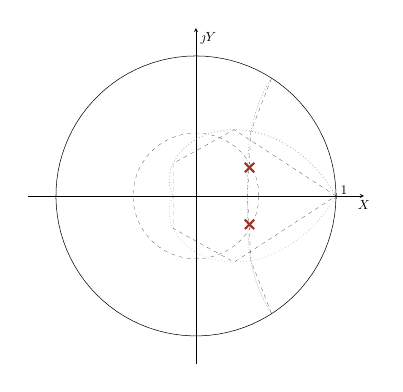
\begin{tikzpicture}[scale=0.48]

\begin{axis}[%
  axis lines=center,
  width=3.5in,
  height=3.5in,
  scale only axis,
  unbounded coords=jump,
  xmin=-1.2,
  xmax=1.2,
  ymin=-1.2,
  ymax=1.2,
  xtick={1},
  ytick=\empty,
  xticklabel style={anchor=south west, draw=none},
  xlabel={$X$},
  ylabel={$\jmath Y$},
  x label style={anchor=north}
]
\addplot [color=black!40, dotted, forget plot]
  table[row sep=crcr]{%
1	0\\
0.994975166457918	0.0086169531277774\\
0.989901329986755	0.0171473087453408\\
0.98477948302476	0.0255910797348211\\
0.979610612912339	0.0339482874654127\\
0.97439570184454	0.0422189617067992\\
0.96913572682452	0.0504031405426052\\
0.963831659617994	0.0585008702838818\\
0.958484466708655	0.0665122053826345\\
0.953095109254565	0.0744372083454012\\
0.947664543045514	0.0822759496468887\\
0.942193718461326	0.0900285076436762\\
0.936683580431134	0.0976949684879922\\
0.931135068393585	0.105275426041575\\
0.925549116258005	0.112769981789622\\
0.919926652366486	0.120178744754836\\
0.914268599456912	0.127501831411582\\
0.90857587462691	0.134739365600147\\
0.902849389298715	0.14189147844113\\
0.89709004918496	0.148958308249953\\
0.891298754255365	0.155940000451509\\
0.88547639870433	0.162836707494953\\
0.879623870919433	0.169648588768638\\
0.873742053450808	0.176375810515214\\
0.867831822981418	0.183018545746879\\
0.8618940502982	0.189576974160811\\
0.855929600264091	0.196051282054771\\
0.849939331790917	0.202441662242887\\
0.843924097813143	0.208748313971631\\
0.837884745262484	0.214971442835991\\
0.831822115043362	0.221111260695846\\
0.825737042009206	0.227167985592546\\
0.819630354939596	0.233141841665717\\
0.81350287651823	0.23903305907027\\
0.807355423311723	0.244841873893657\\
0.801188805749226	0.250568528073344\\
0.795003828102853	0.256213269314532\\
0.78880128846892	0.26177635100812\\
0.782581978749986	0.267258032148917\\
0.776346684637685	0.272658577254117\\
0.770096185596349	0.277978256282022\\
0.763831254847411	0.283217344551051\\
0.757552659354593	0.288376122659003\\
0.751261159809852	0.293454876402612\\
0.744957510620097	0.298453896697378\\
0.738642459894664	0.303373479497687\\
0.732316749433537	0.308213925717227\\
0.725981114716321	0.312975541149701\\
0.719636284891949	0.317658636389843\\
0.71328298276912	0.322263526754741\\
0.706921924807467	0.326790532205477\\
0.700553821109446	0.331239977269081\\
0.694179375412927	0.335612190960806\\
0.687799285084511	0.339907506706737\\
0.681414241113527	0.344126262266724\\
0.675024928106738	0.34826879965765\\
0.668632024283728	0.352335465077047\\
0.662236201472974	0.356326608827046\\
0.65583812510859	0.360242585238686\\
0.649438454227737	0.364083752596562\\
0.643037841468706	0.367850473063845\\
0.636636933069644	0.371543112607646\\
0.630236368867939	0.375162040924758\\
0.623836782300241	0.378707631367759\\
0.617438800403127	0.382180260871485\\
0.611043043814387	0.385580309879881\\
0.604650126774944	0.388908162273233\\
0.598260657131382	0.392164205295778\\
0.591875236339095	0.395348829483698\\
0.585494459466028	0.398462428593512\\
0.579118915197029	0.401505399530848\\
0.572749185838786	0.40447814227962\\
0.566385847325349	0.4073810598316\\
0.560029469224235	0.410214558116388\\
0.553680614743102	0.412979045931794\\
0.547339840736992	0.415674934874619\\
0.541007697716132	0.418302639271854\\
0.534684729854293	0.420862576112287\\
0.528371474997687	0.423355164978523\\
0.522068464674416	0.425780827979435\\
0.515776224104452	0.428139989683019\\
0.509495272210138	0.430433077049683\\
0.503226121627222	0.432660519365961\\
0.496969278716402	0.434822748178651\\
0.490725243575377	0.436920197229388\\
0.484494510051408	0.438953302389643\\
0.478277565754372	0.440922501596166\\
0.472074892070308	0.44282823478686\\
0.465886964175444	0.444670943837092\\
0.459714251050707	0.446451072496453\\
0.453557215496707	0.448169066325949\\
0.447416314149175	0.449825372635651\\
0.441291997494877	0.451420440422779\\
0.435184709887969	0.452954720310238\\
0.429094889566804	0.454428664485608\\
0.423022968671182	0.455842726640584\\
0.416969373260031	0.457197361910859\\
0.410934523329524	0.458493026816478\\
0.404918832831608	0.459730179202636\\
0.398922709692961	0.460909278180935\\
0.392946555834355	0.462030784071105\\
0.386990767190422	0.463095158343177\\
0.381055733729824	0.46410286356012\\
0.375141839475811	0.465054363320948\\
0.369249462527169	0.465950122204273\\
0.363378975079551	0.466790605712337\\
0.357530743447174	0.467576280215505\\
0.351705128084897	0.46830761289722\\
0.345902483610657	0.468985071699428\\
0.34012315882826	0.469609125268472\\
0.334367496750526	0.47018024290145\\
0.328635834622783	0.470698894493046\\
0.322928503946697	0.471165550482829\\
0.317245830504437	0.471580681803022\\
0.311588134383171	0.471944759826739\\
0.305955729999881	0.472258256316704\\
0.300348926126498	0.472521643374422\\
0.294768025915352	0.472735393389845\\
0.289213326924917	0.47289997899149\\
0.283685121145871	0.473015872997045\\
0.278183695027438	0.473083548364434\\
0.272709329504025	0.473103478143368\\
0.267262300022144	0.473076135427362\\
0.261842876567611	0.473001993306221\\
0.256451323693014	0.472881524819009\\
0.251087900545453	0.472715202907487\\
0.24575286089454	0.472503500370018\\
0.240446453160655	0.472246889815953\\
0.235168920443456	0.471945843620488\\
0.229920500550629	0.471600833879988\\
0.224701426026886	0.471212332367794\\
0.219511924183188	0.470780810490488\\
0.214352217126212	0.470306739244642\\
0.209222521788028	0.46979058917403\\
0.204123049956005	0.469232830327317\\
0.199054008302929	0.468633932216212\\
0.194015598417329	0.467994363774097\\
0.189008016834009	0.467314593315119\\
0.184031455064777	0.466595088493758\\
0.179086099629367	0.465836316264853\\
0.174172132086558	0.465038742844109\\
0.169289729065466	0.464202833669053\\
0.16443906229702	0.463329053360474\\
0.159620298645616	0.462417865684317\\
0.154833600140936	0.461469733514039\\
0.150079124009928	0.460485118793442\\
0.145357022708955	0.45946448249995\\
0.140667443956089	0.458408284608366\\
0.136010530763565	0.457316984055071\\
0.131386421470369	0.456191038702701\\
0.126795249774977	0.455030905305267\\
0.122237144768225	0.453837039473741\\
0.117712230966311	0.452609895642096\\
0.113220628343922	0.451349927033798\\
0.108762452367488	0.450057585628759\\
0.104337814028549	0.448733322130736\\
0.0999468198772385	0.447377585935182\\
0.0955895720558732	0.445990825097552\\
0.0912661683326492	0.444573486302051\\
0.0869767021354367	0.443126014830835\\
0.0827212625856707	0.441648854533653\\
0.0784999345323338	0.440142447797942\\
0.0743127985860244	0.438607235519351\\
0.0701599311531092	0.437043657072723\\
0.0660414044699528	0.435452150283505\\
0.0619572866372231	0.433833151399599\\
0.0579076416542657	0.432187095063656\\
0.0538925294535447	0.4305144142858\\
0.0499120059351455	0.428815540416786\\
0.045966123001336	0.42709090312159\\
0.0420549285911806	0.425340930353435\\
0.0381784667152051	0.423566048328237\\
0.0343367774901069	0.421766681499485\\
0.0305298971735083	0.419943252533545\\
0.0267578581987466	0.418096182285383\\
0.0230206892096994	0.416225889774718\\
0.0193184150956407	0.414332792162584\\
0.0156510570261221	0.412417304728323\\
0.0120186324858799	0.410479840846984\\
0.00842115530975893	0.408520811967138\\
0.00485863571765306	0.406540627589113\\
0.00133108034945763	0.404539695243628\\
-0.00216150769996924	0.402518420470845\\
-0.00561912884584125	0.400477206799821\\
-0.00904178697847668	0.39841645572837\\
-0.0124294894283334	0.396336566703324\\
-0.0157822469310498	0.394237937101194\\
-0.0191000735924938	0.39212096220923\\
-0.0223829868538259	0.389986035206885\\
-0.0256310074565762	0.387833547147654\\
-0.028844159407742	0.385663886941331\\
-0.0320224699449067	0.383477441336632\\
-0.035165969501385	0.381274594904221\\
-0.0382746916713966	0.379055730020116\\
-0.0413486731752722	0.37682122684948\\
-0.044387953824694	0.374571463330791\\
-0.0473925764879758	0.372306815160395\\
-0.0503625870553824	0.37002765577743\\
-0.053298034404496	0.367734356349131\\
-0.0561989703656271	0.365427285756506\\
-0.0590654496872782	0.363106810580375\\
-0.0618975300016593	0.360773295087786\\
-0.0646952717902602	0.358427101218792\\
-0.0674587383494818	0.356068588573591\\
-0.0701879957563293	0.353698114400028\\
-0.0728831128341696	0.351316033581455\\
-0.0755441611185572	0.348922698624945\\
-0.078171214823129	0.346518459649865\\
-0.080764350805573	0.344103664376793\\
-0.083323648533672	0.341678658116792\\
-0.0858491900514256	0.339243783761024\\
-0.0883410599452533	0.336799381770708\\
-0.0907993453102799	0.334345790167427\\
-0.0932241357167081	0.331883344523768\\
-0.0956155231762785	0.329412377954299\\
-0.0979736021088205	0.326933221106879\\
-0.100298469308897	0.324446202154309\\
-0.102590223912543	0.3219516467863\\
-0.104848967364106	0.319449878201778\\
-0.107074803383181	0.316941217101503\\
-0.109267837931654	0.314425981681024\\
-0.111428179180845	0.311904487623941\\
-0.113555937478763	0.309377048095487\\
-0.115651225317466	0.306843973736431\\
-0.117714157300535	0.304305572657284\\
-0.119744850110663	0.301762150432819\\
-0.121743422477352	0.299214010096897\\
-0.12370999514474	0.296661452137599\\
-0.125644690839534	0.294104774492655\\
-0.127547634239077	0.29154427254518\\
-0.129418951939533	0.288980239119696\\
-0.131258772424195	0.286412964478459\\
-0.133067226031924	0.283842736318072\\
-0.13484444492572	0.281269839766384\\
-0.136590563061418	0.278694557379684\\
-0.138305716156522	0.27611716914017\\
-0.139990041659173	0.273537952453705\\
-0.141643678717248	0.27095718214785\\
-0.143266768147609	0.268375130470173\\
-0.144859452405477	0.26579206708683\\
-0.146421875553965	0.263208259081419\\
-0.147954183233735	0.260623970954104\\
-0.149456522632818	0.258039464621\\
-0.150929042456566	0.255454999413824\\
-0.152371892897761	0.252870832079808\\
-0.153785225606871	0.250287216781869\\
-0.155169193662457	0.24770440509903\\
-0.156523951541726	0.245122646027102\\
-0.157849655091252	0.242542185979612\\
-0.159146461497839	0.239963268788975\\
-0.160414529259544	0.237386135707918\\
-0.161654018156862	0.234811025411143\\
-0.162865089224069	0.232238173997232\\
-0.164047904720716	0.229667814990784\\
-0.165202628103302	0.227100179344793\\
-0.166329423997092	0.224535495443257\\
-0.167428458168113	0.221973989104012\\
-0.168499897495306	0.219415883581802\\
-0.169543909942848	0.216861399571562\\
-0.170560664532644	0.214310755211935\\
-0.171550331316981	0.211764166088996\\
-0.172513081351356	0.209221845240208\\
-0.173449086667475	0.206684003158576\\
-0.174358520246424	0.204150847797023\\
-0.175241555992005	0.201622584572976\\
-0.176098368704256	0.199099416373151\\
-0.176929134053141	0.196581543558548\\
-0.177734028552409	0.194069163969646\\
-0.178513229533643	0.191562472931801\\
-0.179266915120471	0.189061663260829\\
-0.179995264202967	0.1865669252688\\
-0.180698456412218	0.184078446770007\\
-0.181376672095087	0.181596413087137\\
-0.182030092289137	0.17912100705762\\
-0.18265889869775	0.176652409040165\\
-0.183263273665422	0.17419079692148\\
-0.183843400153239	0.171736346123169\\
-0.184399461714537	0.169289229608803\\
-0.184931642470749	0.16684961789117\\
-0.185440127087425	0.164417679039694\\
-0.185925100750451	0.161993578688022\\
-0.186386749142441	0.159577480041785\\
-0.18682525841932	0.157169543886511\\
-0.18724081518709	0.154769928595712\\
-0.18763360647879	0.152378790139125\\
-0.18800381973163	0.149996282091108\\
-0.188351642764323	0.147622555639199\\
-0.1886772637546	0.145257759592815\\
-0.188980871216915	0.142902040392114\\
-0.189262653980335	0.140555542116997\\
-0.189522801166623	0.138218406496255\\
-0.189761502168506	0.135890772916862\\
-0.189978946628136	0.133572778433407\\
-0.190175324415737	0.131264557777667\\
-0.190350825608445	0.128966243368309\\
-0.190505640469335	0.126677965320734\\
-0.19063995942664	0.124399851457046\\
-0.190753973053159	0.122132027316154\\
-0.19084787204586	0.119874616163997\\
-0.190921847205665	0.117627739003896\\
-0.190976089417432	0.11539151458703\\
-0.191010789630132	0.113166059423026\\
-0.191026138837202	0.110951487790669\\
-0.191022328057108	0.108747911748734\\
-0.190999548314082	0.106555441146921\\
-0.190957990619064	0.104374183636905\\
-0.190897845950822	0.1022042446835\\
-0.190819305237275	0.100045727575919\\
-0.190722559336998	0.0978987334391491\\
-0.190607799020923	0.0957633612454201\\
-0.190475214954231	0.0936397078257795\\
-0.190324997678427	0.0915278678817618\\
-0.190157337593618	0.0894279339971549\\
-0.189972424940972	0.0873399966498598\\
-0.18977044978537	0.0852641442238417\\
-0.18955160199825	0.083200463021171\\
-0.189316071240637	0.0811490372741514\\
-0.189064046946367	0.0791099491575331\\
-0.1887957183055	0.0770832788008092\\
-0.18851127424792	0.0750691043005936\\
-0.18821090342712	0.073067501733078\\
-0.187894794204192	0.0710785451665654\\
-0.187563134631983	0.0691023066740791\\
-0.187216112439458	0.0671388563460452\\
-0.186853915016241	0.065188262303045\\
-0.186476729397344	0.0632505907086381\\
-0.186084742248091	0.0613259057822507\\
-0.185678139849218	0.0594142698121313\\
-0.185257108082164	0.0575157431683673\\
-0.184821832414555	0.0556303843159656\\
-0.18437249788586	0.0537582498279896\\
-0.183909289093245	0.0518993943987567\\
-0.183432390177603	0.0500538708570886\\
-0.182941984809774	0.0482217301796184\\
-0.182438256176944	0.0464030215041461\\
-0.181921386969236	0.044597792143048\\
-0.18139155936647	0.0428060875967306\\
-0.180848955025119	0.041027951567134\\
-0.180293755065441	0.0392634259712775\\
-0.179726140058791	0.0375125509548501\\
-0.179146290015116	0.0357753649058401\\
-0.178554384370631	0.0340519044682056\\
-0.177950601975674	0.032342204555581\\
-0.177335121082737	0.0306462983650213\\
-0.176708119334683	0.0289642173907774\\
-0.176069773753131	0.0272959914381074\\
-0.175420260727028	0.0256416486371157\\
-0.174759756001391	0.0240012154566223\\
-0.174088434666228	0.0223747167180594\\
-0.173406471145636	0.0207621756093928\\
-0.172714039187066	0.0191636136990689\\
-0.172011311850774	0.0175790509499823\\
-0.171298461499436	0.0160085057334652\\
-0.170575659787937	0.0144519948432961\\
-0.16984307765334	0.0129095335097251\\
-0.169100885305011	0.0113811354135165\\
-0.168349252214934	0.00986681270000477\\
-0.167588347108177	0.00836657599316387\\
-0.166818337953539	0.00688043440968819\\
-0.166039391954362	0.00540839557308299\\
-0.165251675539513	0.00395046562776311\\
-0.164455354354524	0.00250664925315921\\
-0.163650593252911	0.00107694967782874\\
};

\addplot [color=black!40, dotted, forget plot, each nth point=10]
  table[row sep=crcr]{%
0.54030230586814	0.841470984807897\\
0.539762693938401	0.840629664537062\\
0.539224460721023	0.83978864621053\\
0.53868760316101	0.838947930597949\\
0.538152118209836	0.838107518462474\\
0.537618002825427	0.837267410560788\\
0.537085253972145	0.836427607643129\\
0.53655386862078	0.835588110453312\\
0.536023843748535	0.83474891972876\\
0.535495176339009	0.833910036200521\\
0.534967863382191	0.833071460593297\\
0.534441901874438	0.832233193625467\\
0.533917288818469	0.831395236009111\\
0.533394021223349	0.830557588450033\\
0.532872096104475	0.829720251647789\\
0.532351510483565	0.828883226295704\\
0.531832261388641	0.828046513080903\\
0.531314345854023	0.827210112684328\\
0.530797760920307	0.826374025780767\\
0.53028250363436	0.825538253038873\\
0.529768571049302	0.82470279512119\\
0.529255960224495	0.823867652684175\\
0.528744668225529	0.823032826378221\\
0.52823469212421	0.822198316847678\\
0.527726028998549	0.821364124730882\\
0.527218675932742	0.820530250660169\\
0.526712630017168	0.819696695261905\\
0.526207888348365	0.818863459156502\\
0.525704448029027	0.818030542958447\\
0.525202306167984	0.817197947276319\\
0.524701459880193	0.816365672712812\\
0.524201906286724	0.815533719864761\\
0.523703642514747	0.814702089323156\\
0.523206665697522	0.813870781673172\\
0.522710972974383	0.813039797494186\\
0.522216561490726	0.8122091373598\\
0.521723428397999	0.811378801837861\\
0.521231570853687	0.810548791490484\\
0.5207409860213	0.809719106874073\\
0.520251671070359	0.808889748539341\\
0.519763623176388	0.808060717031331\\
0.519276839520897	0.80723201288944\\
0.518791317291371	0.806403636647435\\
0.518307053681259	0.805575588833477\\
0.51782404588996	0.80474786997014\\
0.517342291122811	0.803920480574434\\
0.516861786591075	0.803093421157821\\
0.516382529511928	0.802266692226238\\
0.515904517108448	0.80144029428012\\
0.515427746609602	0.800614227814413\\
0.514952215250233	0.799788493318601\\
0.514477920271049	0.79896309127672\\
0.514004858918611	0.798138022167384\\
0.51353302844532	0.797313286463798\\
0.513062426109404	0.796488884633783\\
0.512593049174908	0.795664817139792\\
0.512124894911682	0.794841084438931\\
0.511657960595367	0.794017686982978\\
0.511192243507383	0.793194625218402\\
0.510727740934919	0.792371899586382\\
0.510264450170919	0.791549510522827\\
0.509802368514074	0.790727458458392\\
0.509341493268803	0.7899057438185\\
0.508881821745247	0.789084367023359\\
0.508423351259256	0.788263328487982\\
0.507966079132375	0.787442628622202\\
0.507510002691835	0.786622267830696\\
0.507055119270539	0.785802246512997\\
0.506601426207052	0.784982565063518\\
0.506148920845586	0.784163223871566\\
0.505697600535993	0.78334422332136\\
0.505247462633751	0.782525563792053\\
0.504798504499949	0.781707245657746\\
0.504350723501283	0.780889269287506\\
0.503904117010036	0.780071635045386\\
0.503458682404072	0.779254343290439\\
0.503014417066823	0.77843739437674\\
0.502571318387277	0.777620788653398\\
0.502129383759965	0.776804526464577\\
0.501688610584954	0.775988608149514\\
0.501248996267831	0.775173034042531\\
0.500810538219691	0.774357804473059\\
0.500373233857132	0.773542919765647\\
0.499937080602236	0.772728380239986\\
0.499502075882562	0.771914186210922\\
0.499068217131134	0.771100337988471\\
0.498635501786428	0.770286835877842\\
0.498203927292362	0.769473680179445\\
0.497773491098285	0.768660871188913\\
0.497344190658966	0.767848409197119\\
0.49691602343458	0.767036294490186\\
0.496488986890701	0.766224527349511\\
0.496063078498286	0.765413108051773\\
0.495638295733668	0.764602036868957\\
0.495214636078543	0.763791314068363\\
0.49479209701996	0.762980939912625\\
0.494370676050306	0.762170914659728\\
0.493950370667301	0.761361238563018\\
0.493531178373981	0.760551911871226\\
0.493113096678692	0.759742934828473\\
0.492696123095076	0.758934307674296\\
0.49228025514206	0.758126030643656\\
0.491865490343845	0.757318103966953\\
0.491451826229899	0.756510527870047\\
0.491039260334939	0.755703302574268\\
0.490627790198926	0.754896428296429\\
0.490217413367051	0.754089905248849\\
0.489808127389725	0.753283733639359\\
0.48939992982257	0.75247791367132\\
0.488992818226405	0.751672445543641\\
0.488586790167236	0.750867329450786\\
0.488181843216247	0.750062565582796\\
0.487777974949788	0.749258154125298\\
0.487375182949364	0.748454095259521\\
0.486973464801624	0.747650389162311\\
0.486572818098353	0.746847036006143\\
0.486173240436456	0.746044035959138\\
0.485774729417954	0.745241389185073\\
0.485377282649968	0.744439095843398\\
0.484980897744711	0.743637156089248\\
0.484585572319477	0.742835570073457\\
0.484191303996629	0.742034337942574\\
0.483798090403591	0.74123345983887\\
0.483405929172836	0.740432935900359\\
0.483014817941875	0.739632766260805\\
0.482624754353249	0.738832951049743\\
0.482235736054514	0.738033490392481\\
0.481847760698234	0.737234384410123\\
0.481460825941973	0.736435633219578\\
0.481074929448277	0.735637236933574\\
0.480690068884672	0.734839195660667\\
0.480306241923647	0.734041509505259\\
0.479923446242647	0.733244178567608\\
0.479541679524064	0.732447202943843\\
0.479160939455223	0.73165058272597\\
0.478781223728375	0.730854318001894\\
0.478402530040683	0.730058408855422\\
0.478024856094217	0.729262855366284\\
0.477648199595939	0.728467657610137\\
0.477272558257696	0.727672815658583\\
0.476897929796208	0.726878329579179\\
0.476524311933058	0.726084199435447\\
0.476151702394684	0.725290425286892\\
0.475780098912366	0.724497007189005\\
0.475409499222216	0.723703945193283\\
0.475039901065173	0.722911239347235\\
0.474671302186985	0.722118889694397\\
0.474303700338206	0.721326896274341\\
0.47393709327418	0.720535259122689\\
0.473571478755038	0.719743978271122\\
0.473206854545681	0.718953053747392\\
0.472843218415775	0.718162485575335\\
0.472480568139739	0.71737227377488\\
0.472118901496735	0.716582418362059\\
0.471758216270658	0.715792919349022\\
0.47139851025013	0.715003776744045\\
0.471039781228482	0.71421499055154\\
0.470682027003753	0.713426560772069\\
0.470325245378674	0.712638487402353\\
0.469969434160663	0.71185077043528\\
0.46961459116181	0.71106340985992\\
0.469260714198871	0.710276405661534\\
0.468907801093259	0.709489757821582\\
0.46855584967103	0.708703466317736\\
0.468204857762879	0.70791753112389\\
0.467854823204124	0.707131952210168\\
0.467505743834703	0.706346729542938\\
0.467157617499157	0.705561863084818\\
0.46681044204663	0.704777352794687\\
0.46646421533085	0.703993198627698\\
0.466118935210123	0.703209400535282\\
0.465774599547328	0.702425958465164\\
0.465431206209898	0.701642872361368\\
0.46508875306982	0.700860142164228\\
0.46474723800362	0.700077767810399\\
0.464406658892354	0.699295749232865\\
0.464067013621601	0.698514086360948\\
0.463728300081451	0.697732779120317\\
0.463390516166498	0.696951827433\\
0.463053659775829	0.69617123121739\\
0.462717728813013	0.695390990388255\\
0.462382721186096	0.694611104856748\\
0.462048634807588	0.693831574530415\\
0.461715467594456	0.693052399313204\\
0.461383217468113	0.692273579105474\\
0.46105188235441	0.691495113804002\\
0.460721460183626	0.690717003301996\\
0.460391948890459	0.689939247489099\\
0.460063346414016	0.6891618462514\\
0.459735650697807	0.68838479947144\\
0.459408859689731	0.687608107028223\\
0.459082971342071	0.686831768797225\\
0.458757983611482	0.686055784650399\\
0.458433894458983	0.685280154456184\\
0.45811070184995	0.684504878079514\\
0.457788403754102	0.683729955381828\\
0.457466998145497	0.682955386221072\\
0.457146483002521	0.682181170451714\\
0.456826856307877	0.681407307924745\\
0.45650811604858	0.680633798487693\\
0.456190260215944	0.679860641984627\\
0.455873286805575	0.679087838256163\\
0.455557193817364	0.678315387139476\\
0.455241979255474	0.677543288468305\\
0.454927641128334	0.676771542072959\\
0.454614177448629	0.676000147780328\\
0.454301586233291	0.675229105413887\\
0.453989865503491	0.674458414793703\\
0.45367901328463	0.673688075736445\\
0.453369027606329	0.672918088055388\\
0.453059906502422	0.672148451560422\\
0.452751648010945	0.671379166058059\\
0.452444250174131	0.670610231351436\\
0.452137711038396	0.669841647240328\\
0.451832028654334	0.669073413521148\\
0.451527201076709	0.668305529986959\\
0.451223226364442	0.667537996427477\\
0.450920102580607	0.666770812629081\\
0.45061782779242	0.666003978374815\\
0.45031640007123	0.665237493444396\\
0.450015817492511	0.664471357614223\\
0.449716078135855	0.663705570657378\\
0.449417180084962	0.662940132343639\\
0.449119121427628	0.662175042439477\\
0.448821900255744	0.66141030070807\\
0.448525514665281	0.660645906909305\\
0.448229962756284	0.659881860799785\\
0.447935242632865	0.659118162132834\\
0.44764135240319	0.658354810658502\\
0.447348290179475	0.657591806123574\\
0.447056054077976	0.65682914827157\\
0.44676464221898	0.656066836842755\\
0.446474052726798	0.655304871574145\\
0.446184283729755	0.654543252199506\\
0.445895333360182	0.653781978449367\\
0.445607199754407	0.65302105005102\\
0.445319881052752	0.652260466728527\\
0.445033375399515	0.651500228202724\\
0.444747680942969	0.650740334191229\\
0.444462795835354	0.649980784408442\\
0.444178718232864	0.649221578565555\\
0.443895446295641	0.648462716370551\\
0.443612978187767	0.647704197528215\\
0.443331312077259	0.646946021740133\\
0.443050446136053	0.6461881887047\\
0.442770378540003	0.645430698117124\\
0.44249110746887	0.644673549669429\\
0.442212631106314	0.643916743050459\\
0.441934947639884	0.643160277945886\\
0.441658055261015	0.64240415403821\\
0.441381952165015	0.641648371006764\\
0.441106636551058	0.64089292852772\\
0.440832106622177	0.640137826274091\\
0.440558360585258	0.639383063915734\\
0.440285396651025	0.638628641119359\\
0.44001321303404	0.637874557548525\\
0.43974180795269	0.63712081286365\\
0.439471179629181	0.636367406722011\\
0.439201326289529	0.63561433877775\\
0.438932246163553	0.634861608681876\\
0.438663937484865	0.634109216082268\\
0.438396398490867	0.633357160623679\\
0.438129627422738	0.632605441947739\\
0.437863622525426	0.631854059692959\\
0.437598382047645	0.631103013494734\\
0.437333904241863	0.630352302985342\\
0.437070187364295	0.629601927793954\\
0.436807229674897	0.628851887546632\\
0.436545029437354	0.628102181866332\\
0.436283584919079	0.627352810372908\\
0.436022894391196	0.626603772683115\\
0.435762956128542	0.625855068410611\\
0.435503768409653	0.625106697165959\\
0.435245329516757	0.624358658556628\\
0.434987637735768	0.623610952186999\\
0.434730691356278	0.622863577658366\\
0.434474488671548	0.622116534568935\\
0.434219027978502	0.621369822513831\\
0.433964307577718	0.620623441085097\\
0.433710325773422	0.619877389871695\\
0.433457080873477	0.619131668459512\\
0.433204571189379	0.618386276431358\\
0.43295279503625	0.617641213366968\\
0.432701750732826	0.616896478843007\\
0.432451436601452	0.616152072433068\\
0.432201850968076	0.615407993707675\\
0.431952992162239	0.614664242234284\\
0.431704858517069	0.613920817577285\\
0.431457448369273	0.613177719298002\\
0.431210760059128	0.612434946954695\\
0.430964791930477	0.611692500102562\\
0.430719542330718	0.610950378293739\\
0.4304750096108	0.610208581077301\\
0.430231192125212	0.609467107999262\\
0.429988088231978	0.608725958602578\\
0.429745696292648	0.607985132427146\\
0.429504014672294	0.607244629009805\\
0.429263041739498	0.606504447884337\\
0.429022775866347	0.605764588581468\\
0.428783215428427	0.605025050628865\\
0.428544358804814	0.604285833551141\\
0.428306204378065	0.603546936869854\\
0.428068750534215	0.602808360103502\\
0.427831995662766	0.602070102767534\\
0.427595938156682	0.601332164374336\\
0.427360576412381	0.600594544433245\\
0.427125908829728	0.599857242450537\\
0.426891933812026	0.599120257929434\\
0.426658649766011	0.598383590370103\\
0.426426055101846	0.59764723926965\\
0.426194148233109	0.596911204122128\\
0.425962927576792	0.596175484418529\\
0.425732391553288	0.595440079646789\\
0.425502538586388	0.594704989291781\\
0.425273367103272	0.59397021283532\\
0.425044875534504	0.593235749756162\\
0.424817062314021	0.592501599529995\\
0.42458992587913	0.59176776162945\\
0.424363464670499	0.59103423552409\\
0.424137677132149	0.590301020680412\\
0.42391256171145	0.589568116561847\\
0.423688116859112	0.58883552262876\\
0.423464341029178	0.58810323833844\\
0.423241232679015	0.587371263145111\\
0.423018790269314	0.586639596499918\\
0.422797012264074	0.585908237850935\\
0.422575897130603	0.585177186643157\\
0.422355443339504	0.584446442318501\\
0.422135649364675	0.583716004315801\\
0.421916513683297	0.582985872070811\\
0.421698034775829	0.582256045016197\\
0.421480211126001	0.581526522581538\\
0.421263041220808	0.580797304193323\\
0.421046523550503	0.58006838927495\\
0.420830656608586	0.579339777246718\\
0.420615438891806	0.578611467525831\\
0.420400868900144	0.577883459526392\\
0.420186945136815	0.5771557526594\\
0.419973666108256	0.576428346332746\\
0.41976103032412	0.575701239951214\\
0.419549036297272	0.574974432916473\\
0.419337682543778	0.574247924627077\\
0.419126967582901	0.57352171447846\\
0.418916889937096	0.572795801862935\\
0.418707448131999	0.572070186169684\\
0.418498640696424	0.571344866784765\\
0.418290466162353	0.570619843091098\\
0.418082923064934	0.569895114468466\\
0.417876009942469	0.569170680293511\\
0.417669725336412	0.56844653993973\\
0.41746406779136	0.567722692777469\\
0.417259035855045	0.566999138173921\\
0.417054628078333	0.56627587549312\\
0.416850843015211	0.565552904095938\\
0.416647679222784	0.564830223340079\\
0.416445135261268	0.564107832580074\\
0.416243209693983	0.56338573116728\\
0.416041901087346	0.562663918449871\\
0.415841208010867	0.561942393772834\\
0.415641129037138	0.561221156477965\\
0.415441662741833	0.560500205903863\\
0.415242807703694	0.559779541385926\\
0.415044562504532	0.559059162256343\\
0.414846925729215	0.558339067844093\\
0.414649895965663	0.557619257474932\\
0.414453471804843	0.556899730471397\\
0.414257651840763	0.556180486152791\\
0.414062434670464	0.555461523835183\\
0.413867818894012	0.554742842831401\\
0.413673803114496	0.554024442451023\\
0.413480385938019	0.553306322000374\\
0.413287565973692	0.552588480782517\\
0.413095341833629	0.55187091809725\\
0.412903712132937	0.551153633241096\\
0.412712675489714	0.550436625507298\\
0.412522230525041	0.549719894185811\\
0.412332375862976	0.549003438563298\\
0.412143110130546	0.548287257923117\\
0.411954431957746	0.547571351545322\\
0.411766339977524	0.546855718706648\\
0.411578832825784	0.546140358680509\\
0.411391909141374	0.545425270736987\\
0.411205567566082	0.544710454142827\\
0.411019806744629	0.543995908161427\\
0.410834625324664	0.543281632052833\\
0.410650021956757	0.542567625073726\\
0.410465995294393	0.541853886477419\\
0.410282543993964	0.541140415513847\\
0.410099666714769	0.540427211429558\\
0.409917362119	0.539714273467703\\
0.409735628871742	0.539001600868033\\
0.409554465640962	0.538289192866882\\
0.409373871097508	0.537577048697166\\
0.409193843915101	0.536865167588369\\
0.409014382770325	0.536153548766536\\
0.408835486342629	0.535442191454261\\
0.408657153314313	0.534731094870683\\
0.408479382370527	0.534020258231471\\
0.408302172199265	0.533309680748816\\
0.408125521491354	0.532599361631423\\
0.407949428940455	0.531889300084499\\
0.407773893243052	0.531179495309743\\
0.407598913098449	0.530469946505337\\
0.407424487208762	0.529760652865935\\
0.407250614278914	0.529051613582652\\
0.40707729301663	0.528342827843053\\
0.406904522132429	0.527634294831145\\
0.406732300339621	0.526926013727362\\
0.406560626354297	0.526217983708558\\
0.40638949889533	0.525510203947991\\
0.40621891668436	0.524802673615316\\
0.406048878445796	0.524095391876573\\
0.405879382906807	0.523388357894171\\
0.405710428797317	0.522681570826882\\
0.405542014849996	0.521975029829825\\
0.40537413980026	0.521268734054456\\
0.405206802386261	0.520562682648553\\
0.405040001348882	0.519856874756209\\
0.404873735431734	0.519151309517812\\
0.404708003381144	0.518445986070039\\
0.404542803946157	0.517740903545838\\
0.404378135878525	0.51703606107442\\
0.404213997932703	0.51633145778124\\
0.404050388865844	0.515627092787988\\
0.403887307437792	0.514922965212575\\
0.403724752411077	0.514219074169115\\
0.403562722550909	0.513515418767917\\
0.403401216625174	0.512811998115469\\
0.403240233404426	0.51210881131442\\
0.403079771661883	0.511405857463572\\
0.40291983017342	0.510703135657861\\
0.402760407717566	0.510000644988341\\
0.402601503075495	0.509298384542175\\
0.402443115031024	0.508596353402615\\
0.402285242370605	0.507894550648989\\
0.402127883883318	0.507192975356682\\
0.401971038360872	0.506491626597125\\
0.401814704597591	0.505790503437778\\
0.401658881390416	0.505089604942113\\
0.401503567538893	0.504388930169596\\
0.401348761845173	0.503688478175676\\
0.401194463114003	0.502988248011761\\
0.401040670152722	0.50228823872521\\
0.400887381771257	0.501588449359308\\
0.400734596782113	0.500888878953255\\
0.400582314000372	0.500189526542143\\
0.400430532243686	0.499490391156944\\
0.400279250332273	0.49879147182449\\
0.400128467088907	0.498092767567452\\
0.399978181338919	0.497394277404329\\
0.399828391910187	0.496696000349422\\
0.399679097633134	0.495997935412819\\
0.399530297340718	0.495300081600379\\
0.399381989868431	0.494602437913709\\
0.399234174054294	0.493905003350143\\
0.399086848738846	0.49320777690273\\
0.398940012765147	0.492510757560208\\
0.398793664978765	0.491813944306987\\
0.398647804227776	0.491117336123128\\
0.398502429362755	0.490420931984323\\
0.398357539236775	0.489724730861874\\
0.398213132705398	0.489028731722674\\
0.39806920862667	0.488332933529185\\
0.397925765861118	0.487637335239415\\
0.397782803271744	0.486941935806902\\
0.39764031972402	0.486246734180684\\
0.39749831408588	0.485551729305286\\
0.397356785227718	0.484856920120692\\
0.397215732022384	0.484162305562325\\
0.397075153345175	0.483467884561025\\
0.396935048073831	0.482773656043023\\
0.396795415088531	0.482079618929922\\
0.396656253271888	0.481385772138671\\
0.396517561508943	0.480692114581542\\
0.396379338687161	0.479998645166107\\
0.396241583696423	0.479305362795214\\
0.396104295429024	0.478612266366961\\
0.395967472779668	0.477919354774671\\
0.395831114645461	0.477226626906872\\
0.395695219925906	0.476534081647265\\
0.395559787522899	0.475841717874705\\
0.395424816340726	0.475149534463171\\
0.395290305286053	0.47445753028174\\
0.395156253267925	0.473765704194565\\
0.395022659197758	0.473074055060844\\
0.39488952198934	0.472382581734794\\
0.394756840558816	0.471691283065628\\
0.394624613824694	0.47100015789752\\
0.394492840707832	0.470309205069586\\
0.394361520131436	0.46961842341585\\
0.394230651021055	0.468927811765217\\
0.394100232304577	0.468237368941446\\
0.393970262912223	0.467547093763121\\
0.393840741776541	0.466856985043618\\
0.393711667832403	0.466167041591083\\
0.393583040017001	0.465477262208394\\
0.393454857269837	0.464787645693136\\
0.393327118532725	0.464098190837569\\
0.393199822749781	0.4634088964286\\
0.393072968867421	0.462719761247745\\
0.392946555834355	0.462030784071105\\
0.392820582601581	0.461341963669332\\
0.392695048122384	0.460653298807593\\
0.392569951352326	0.459964788245545\\
0.392445291249246	0.459276430737294\\
0.392321066773252	0.458588225031369\\
0.392197276886717	0.457900169870683\\
0.392073920554277	0.457212263992505\\
0.39195099674282	0.456524506128419\\
0.391828504421489	0.455836895004296\\
0.391706442561671	0.455149429340254\\
0.391584810136995	0.454462107850625\\
0.391463606123327	0.453774929243921\\
0.391342829498766	0.453087892222794\\
0.391222479243636	0.452400995484003\\
0.391102554340488	0.451714237718375\\
0.390983053774088	0.451027617610771\\
0.390863976531415	0.450341133840043\\
0.39074532160166	0.449654785079001\\
0.390627087976215	0.448968569994374\\
0.390509274648673	0.448282487246767\\
0.390391880614822	0.447596535490627\\
0.39027490487264	0.4469107133742\\
0.39015834642229	0.446225019539494\\
0.390042204266118	0.445539452622235\\
0.389926477408644	0.444854011251828\\
0.389811164856562	0.444168694051316\\
0.389696265618732	0.443483499637336\\
0.389581778706177	0.442798426620081\\
0.389467703132079	0.442113473603252\\
0.389354037911772	0.44142863918402\\
0.389240782062742	0.440743921952978\\
0.389127934604617	0.4400593204941\\
0.389015494559166	0.439374833384694\\
0.388903460950293	0.438690459195361\\
0.388791832804034	0.438006196489943\\
0.388680609148552	0.437322043825484\\
0.38856978901413	0.436637999752179\\
0.388459371433172	0.435954062813327\\
0.388349355440191	0.435270231545288\\
0.388239740071813	0.434586504477429\\
0.388130524366765	0.433902880132079\\
0.388021707365875	0.433219357024479\\
0.387913288112068	0.432535933662733\\
0.387805265650358	0.431852608547757\\
0.387697639027846	0.43116938017323\\
0.387590407293716	0.43048624702554\\
0.387483569499229	0.429803207583734\\
0.38737712469772	0.429120260319467\\
0.387271071944593	0.428437403696945\\
0.387165410297317	0.427754636172876\\
0.387060138815421	0.427071956196414\\
0.38695525656049	0.426389362209102\\
0.386850762596162	0.425706852644822\\
0.38674665598812	0.425024425929735\\
0.386642935804091	0.424342080482224\\
0.386539601113843	0.423659814712842\\
0.386436650989175	0.422977627024248\\
0.38633408450392	0.422295515811153\\
0.386231900733932	0.421613479460259\\
0.386130098757092	0.420931516350199\\
0.386028677653294	0.42024962485148\\
0.385927636504448	0.419567803326417\\
0.385826974394472	0.418886050129075\\
0.385726690409287	0.418204363605205\\
0.385626783636818	0.417522742092183\\
0.385527253166984	0.416841183918943\\
0.385428098091694	0.416159687405916\\
0.385329317504849	0.415478250864961\\
0.385230910502332	0.414796872599304\\
0.385132876182003	0.414115550903467\\
0.385035213643701	0.413434284063202\\
0.384937921989234	0.412753070355424\\
0.384841000322377	0.412071908048142\\
0.384744447748868	0.411390795400386\\
0.384648263376404	0.410709730662142\\
0.384552446314637	0.410028712074277\\
0.384456995675168	0.409347737868467\\
0.384361910571546	0.408666806267126\\
0.384267190119259	0.407985915483331\\
0.384172833435737	0.407305063720748\\
0.384078839640342	0.406624249173555\\
0.383985207854366	0.405943470026369\\
0.383891937201027	0.405262724454166\\
0.383799026805465	0.404582010622205\\
0.383706475794738	0.403901326685946\\
0.383614283297815	0.403220670790976\\
0.38352244844558	0.40254004107292\\
0.383430970370817	0.401859435657368\\
0.383339848208215	0.401178852659787\\
0.38324908109436	0.400498290185438\\
0.383158668167731	0.399817746329295\\
0.383068608568697	0.399137219175953\\
0.382978901439512	0.39845670679955\\
0.382889545924312	0.397776207263671\\
0.382800541169111	0.397095718621266\\
0.382711886321796	0.396415238914558\\
0.382623580532124	0.39573476617495\\
0.382535622951719	0.395054298422939\\
0.382448012734064	0.394373833668017\\
0.382360749034503	0.393693369908582\\
0.382273831010232	0.393012905131842\\
0.382187257820298	0.392332437313717\\
0.382101028625594	0.391651964418743\\
0.382015142588854	0.390971484399974\\
0.381929598874653	0.390290995198883\\
0.381844396649398	0.38961049474526\\
0.381759535081328	0.388929980957112\\
0.381675013340508	0.388249451740556\\
0.381590830598827	0.38756890498972\\
0.381506986029992	0.386888338586634\\
0.381423478809526	0.386207750401122\\
0.381340308114762	0.3855271382907\\
0.381257473124843	0.384846500100458\\
0.381174973020713	0.384165833662956\\
0.381092806985117	0.383485136798108\\
0.381010974202598	0.382804407313071\\
0.380929473859488	0.382123643002129\\
0.38084830514391	0.381442841646577\\
0.380767467245771	0.380762001014603\\
0.380686959356758	0.380081118861167\\
0.380606780670337	0.379400192927887\\
0.380526930381746	0.378719220942907\\
0.380447407687995	0.378038200620784\\
0.380368211787857	0.377357129662353\\
0.380289341881869	0.376676005754608\\
0.380210797172326	0.375994826570569\\
0.380132576863278	0.375313589769156\\
0.380054680160527	0.374632292995054\\
0.37997710627162	0.373950933878582\\
0.379899854405851	0.373269510035555\\
0.379822923774251	0.372588019067155\\
0.379746313589589	0.371906458559785\\
0.379670023066367	0.371224826084931\\
0.379594051420814	0.370543119199023\\
0.379518397870887	0.369861335443291\\
0.379443061636263	0.369179472343616\\
0.379368041938338	0.368497527410386\\
0.379293338000221	0.367815498138347\\
0.379218949046733	0.367133382006451\\
0.379144874304403	0.366451176477703\\
0.379071113001461	0.365768878999008\\
0.37899766436784	0.36508648700101\\
0.378924527635168	0.364403997897939\\
0.378851702036765	0.363721409087443\\
0.378779186807642	0.363038717950432\\
0.378706981184494	0.362355921850909\\
0.378635084405699	0.361673018135801\\
0.378563495711313	0.360990004134794\\
0.378492214343068	0.360306877160158\\
0.378421239544366	0.359623634506574\\
0.378350570560279	0.358940273450957\\
0.378280206637541	0.35825679125228\\
0.378210147024547	0.357573185151387\\
0.378140390971353	0.356889452370817\\
0.378070937729664	0.356205590114612\\
0.378001786552838	0.355521595568135\\
0.37793293669588	0.35483746589787\\
0.377864387415437	0.354153198251239\\
0.377796137969796	0.353468789756396\\
0.377728187618882	0.352784237522037\\
0.377660535624252	0.352099538637192\\
0.377593181249092	0.351414690171024\\
0.377526123758214	0.350729689172624\\
0.377459362418054	0.350044532670794\\
0.377392896496666	0.349359217673844\\
0.377326725263721	0.348673741169368\\
0.377260847990499	0.347988100124031\\
0.377195263949893	0.347302291483345\\
0.377129972416399	0.346616312171444\\
0.377064972666117	0.345930159090859\\
0.377000263976743	0.345243829122282\\
0.376935845627572	0.344557319124338\\
0.376871716899487	0.343870625933344\\
0.376807877074962	0.343183746363069\\
0.376744325438057	0.342496677204488\\
0.376681061274411	0.341809415225537\\
0.376618083871243	0.341121957170863\\
0.376555392517349	0.340434299761564\\
0.376492986503093	0.339746439694935\\
0.376430865120411	0.339058373644207\\
0.376369027662802	0.338370098258277\\
0.376307473425328	0.337681610161441\\
0.37624620170461	0.33699290595312\\
0.376185211798823	0.336303982207584\\
0.376124503007693	0.335614835473666\\
0.376064074632498	0.334925462274484\\
0.376003925976059	0.334235859107143\\
0.375944056342739	0.333546022442447\\
0.375884465038442	0.332855948724598\\
0.375825151370604	0.332165634370895\\
0.375766114648197	0.331475075771423\\
0.375707354181721	0.330784269288746\\
0.3756488692832	0.33009321125759\\
0.375590659266182	0.329401897984517\\
0.375532723445736	0.328710325747605\\
0.375475061138444	0.328018490796116\\
0.375417671662403	0.327326389350157\\
0.375360554337219	0.326634017600341\\
0.375303708484006	0.325941371707444\\
0.37524713342538	0.325248447802048\\
0.375190828485456	0.32455524198419\\
0.375134792989849	0.323861750322997\\
0.375079026265665	0.323167968856317\\
0.375023527641503	0.32247389359035\\
0.374968296447448	0.321779520499264\\
0.374913332015069	0.321084845524814\\
0.374858633677417	0.32038986457595\\
0.374804200769022	0.319694573528419\\
0.374750032625887	0.318998968224362\\
0.374696128585488	0.318303044471906\\
0.374642487986769	0.317606798044745\\
0.37458911017014	0.316910224681722\\
0.374535994477473	0.316213320086395\\
0.374483140252101	0.315516079926602\\
0.37443054683881	0.314818499834022\\
0.374378213583842	0.314120575403719\\
0.374326139834889	0.313422302193687\\
0.374274324941088	0.312723675724387\\
0.374222768253021	0.312024691478272\\
0.374171469122712	0.311325344899309\\
0.37412042690362	0.310625631392488\\
0.374069640950642	0.309925546323332\\
0.374019110620105	0.309225085017387\\
0.373968835269765	0.308524242759712\\
0.373918814258803	0.307823014794359\\
0.373869046947824	0.307121396323845\\
0.37381953269885	0.306419382508609\\
0.373770270875324	0.305716968466471\\
0.373721260842097	0.305014149272069\\
0.373672501965436	0.3043109199563\\
0.373623993613012	0.303607275505741\\
0.373575735153902	0.302903210862063\\
0.373527725958584	0.30219872092144\\
0.373479965398935	0.301493800533939\\
0.373432452848228	0.300788444502909\\
0.373385187681128	0.300082647584354\\
0.37333816927369	0.299376404486292\\
0.373291397003357	0.298669709868113\\
0.373244870248953	0.297962558339916\\
0.373198588390686	0.297254944461841\\
0.37315255081014	0.296546862743382\\
0.373106756890275	0.295838307642699\\
0.373061206015423	0.295129273565906\\
0.373015897571285	0.294419754866355\\
0.372970830944928	0.2937097458439\\
0.372926005524784	0.292999240744158\\
0.372881420700642	0.292288233757746\\
0.372837075863654	0.291576719019509\\
0.372792970406321	0.290864690607737\\
0.3727491037225	0.290152142543361\\
0.372705475207395	0.28943906878914\\
0.372662084257558	0.288725463248833\\
0.372618930270881	0.28801131976635\\
0.3725760126466	0.287296632124895\\
0.372533330785286	0.286581394046088\\
0.372490884088846	0.28586559918907\\
0.372448671960518	0.285149241149599\\
0.372406693804871	0.284432313459118\\
0.372364949027797	0.283714809583816\\
0.372323437036515	0.28299672292366\\
0.372282157239562	0.282278046811424\\
0.372241109046793	0.28155877451168\\
0.37220029186938	0.280838899219789\\
0.372159705119805	0.280118414060861\\
0.372119348211861	0.279397312088694\\
0.372079220560646	0.278675586284701\\
0.372039321582563	0.277953229556813\\
0.371999650695315	0.277230234738351\\
0.371960207317906	0.276506594586892\\
0.371920990870632	0.275782301783101\\
0.371882000775084	0.275057348929544\\
0.371843236454142	0.274331728549476\\
0.371804697331975	0.273605433085609\\
0.371766382834034	0.272878454898846\\
0.371728292387053	0.272150786267004\\
0.371690425419047	0.271422419383494\\
0.371652781359303	0.270693346355991\\
0.371615359638387	0.269963559205061\\
0.371578159688132	0.269233049862775\\
0.37154118094164	0.268501810171284\\
0.37150442283328	0.267769831881368\\
0.371467884798682	0.267037106650954\\
0.371431566274738	0.266303626043605\\
0.371395466699595	0.265569381526977\\
0.371359585512659	0.264834364471242\\
0.371323922154583	0.264098566147477\\
0.371288476067274	0.263361977726022\\
0.371253246693882	0.2626245902748\\
0.371218233478804	0.261886394757605\\
0.371183435867678	0.261147382032347\\
0.37114885330738	0.260407542849263\\
0.371114485246022	0.259666867849091\\
0.371080331132951	0.258925347561198\\
0.371046390418744	0.258182972401673\\
0.371012662555207	0.257439732671377\\
0.37097914699537	0.256695618553942\\
0.370945843193489	0.255950620113742\\
0.370912750605038	0.255204727293796\\
0.370879868686711	0.254457929913647\\
0.370847196896416	0.253710217667177\\
0.370814734693273	0.252961580120379\\
0.370782481537614	0.252212006709075\\
0.370750436890978	0.251461486736587\\
0.370718600216109	0.250710009371349\\
0.370686970976953	0.249957563644464\\
0.370655548638655	0.24920413844721\\
0.37062433266756	0.248449722528478\\
0.370593322531206	0.24769430449216\\
0.370562517698324	0.246937872794467\\
0.370531917638833	0.246180415741187\\
0.370501521823841	0.24542192148488\\
0.37047132972564	0.244662378021997\\
0.370441340817705	0.243901773189943\\
0.370411554574688	0.243140094664053\\
0.370381970472421	0.242377329954507\\
0.370352587987909	0.241613466403164\\
0.37032340659933	0.240848491180316\\
0.370294425786031	0.240082391281366\\
0.370265645028525	0.23931515352342\\
0.370237063808491	0.238546764541796\\
0.370208681608771	0.23777721078644\\
0.370180497913365	0.237006478518261\\
0.37015251220743	0.236234553805359\\
0.370124723977278	0.23546142251917\\
0.370097132710374	0.234687070330501\\
0.370069737895333	0.233911482705469\\
0.370042539021915	0.233134644901329\\
0.370015535581028	0.232356541962199\\
0.36998872706472	0.231577158714665\\
0.36996211296618	0.230796479763275\\
0.369935692779735	0.230014489485909\\
0.369909466000846	0.229231172029028\\
0.369883432126107	0.228446511302792\\
0.369857590653244	0.227660490976047\\
0.369831941081108	0.226873094471176\\
0.369806482909677	0.226084304958802\\
0.369781215640053	0.225294105352357\\
0.369756138774458	0.224502478302486\\
0.369731251816231	0.223709406191306\\
0.369706554269828	0.222914871126492\\
0.369682045640819	0.222118854935208\\
0.369657725435885	0.221321339157854\\
0.369633593162815	0.22052230504164\\
0.369609648330504	0.219721733533971\\
0.369585890448953	0.218919605275644\\
0.369562319029263	0.218115900593838\\
0.369538933583636	0.21731059949491\\
0.369515733625368	0.216503681656961\\
0.369492718668853	0.215695126422198\\
0.369469888229576	0.214884912789054\\
0.369447241824111	0.214073019404076\\
0.369424778970121	0.213259424553562\\
0.369402499186354	0.212444106154945\\
0.36938040199264	0.211627041747911\\
0.369358486909892	0.210808208485241\\
0.3693367534601	0.209987583123366\\
0.369315201166329	0.209165142012623\\
0.36929382955272	0.208340861087209\\
0.369272638144484	0.207514715854803\\
0.369251626467901	0.206686681385867\\
0.369230794050319	0.205856732302592\\
0.369210140420151	0.205024842767486\\
0.369189665106871	0.204190986471587\\
0.369169367641014	0.203355136622287\\
0.369149247554172	0.202517265930751\\
0.369129304378993	0.201677346598912\\
0.36910953764918	0.200835350306022\\
0.369089946899484	0.199991248194758\\
0.369070531665707	0.199145010856834\\
0.369051291484697	0.19829660831813\\
0.369032225894347	0.197446010023291\\
0.369013334433591	0.196593184819795\\
0.368994616642403	0.195738100941449\\
0.368976072061795	0.194880725991301\\
0.368957700233815	0.194021026923938\\
0.368939500701544	0.193158970027136\\
0.368921473009093	0.192294520902846\\
0.368903616701604	0.191427644447482\\
0.368885931325242	0.190558304831462\\
0.368868416427201	0.189686465478007\\
0.368851071555694	0.188812089041114\\
0.368833896259956	0.187935137382709\\
0.368816890090237	0.187055571548916\\
0.368800052597805	0.186173351745405\\
0.368783383334942	0.185288437311783\\
0.368766881854941	0.184400786694969\\
0.368750547712102	0.183510357421519\\
0.368734380461735	0.182617106068834\\
0.368718379660153	0.181720988235212\\
0.368702544864672	0.180821958508667\\
0.36868687563361	0.179919970434472\\
0.368671371526282	0.179014976481355\\
0.368656032102999	0.178106928006267\\
0.368640856925068	0.177195775217669\\
0.368625845554786	0.176281467137245\\
0.368610997555442	0.175363951559965\\
0.36859631249131	0.174443175012407\\
0.368581789927653	0.173519082709248\\
0.368567429430716	0.172591618507822\\
0.368553230567724	0.171660724860641\\
0.368539192906884	0.170726342765767\\
0.368525316017378	0.169788411714908\\
0.368511599469366	0.16884686963912\\
0.368498042833979	0.167901652851974\\
0.368484645683318	0.166952695990042\\
0.368471407590457	0.165999931950538\\
0.368458328129432	0.165043291825968\\
0.368445406875247	0.164082704835585\\
0.368432643403868	0.163118098253477\\
0.368420037292221	0.162149397333074\\
0.368407588118192	0.161176525227855\\
0.368395295460621	0.160199402908021\\
0.368383158899307	0.159217949072881\\
0.368371178014996	0.158232080058674\\
0.368359352389388	0.157241709741542\\
0.368347681605131	0.156246749435325\\
0.368336165245818	0.155247107783853\\
0.368324802895988	0.154242690647358\\
0.368313594141121	0.153233400982614\\
0.368302538567639	0.152219138716371\\
0.368291635762899	0.151199800611629\\
0.368280885315198	0.150175280126245\\
0.368270286813765	0.149145467263324\\
0.368259839848761	0.148110248412818\\
0.36824954401128	0.147069506183681\\
0.368239398893341	0.146023119225891\\
0.368229404087892	0.144970962041572\\
0.368219559188802	0.143912904784408\\
0.368209863790866	0.142848813046427\\
0.368200317489797	0.141778547631191\\
0.368190919882227	0.140701964312307\\
0.368181670565704	0.139618913576087\\
0.368172569138691	0.138529240347058\\
0.368163615200564	0.13743278369493\\
0.368154808351608	0.136329376521432\\
0.368146148193017	0.13521884522534\\
0.368137634326893	0.134101009343784\\
0.36812926635624	0.132975681167763\\
0.368121043884968	0.131842665329573\\
0.368112966517885	0.130701758359581\\
0.3681050338607	0.129552748209534\\
0.368097245520016	0.128395413739267\\
0.368089601103335	0.127229524163301\\
0.368082100219049	0.126054838453448\\
0.368074742476442	0.124871104693086\\
0.368067527485688	0.123678059378209\\
0.368060454857847	0.122475426659834\\
0.368053524204865	0.121262917521612\\
0.368046735139573	0.120040228885755\\
0.368040087275681	0.118807042639501\\
0.368033580227781	0.11756302457331\\
0.368027213611341	0.116307823220823\\
0.368020987042707	0.115041068589238\\
0.368014900139097	0.113762370767209\\
0.368008952518604	0.112471318395502\\
0.368003143800188	0.11116747698352\\
0.367997473603679	0.109850387052287\\
0.367991941549774	0.108519562081537\\
0.367986547260036	0.107174486235047\\
0.367981290356887	0.105814611834237\\
0.367976170463614	0.104439356545167\\
0.367971187204362	0.103048100238158\\
0.367966340204131	0.101640181472294\\
0.36796162908878	0.100214893548549\\
0.367957053485019	0.0987714800650799\\
0.367952613020412	0.0973091298957599\\
0.367948307323372	0.0958269714978085\\
0.36794413602316	0.0943240664356579\\
0.367940098749883	0.0927994019850621\\
0.367936195134494	0.0912518826526587\\
0.367932424808787	0.0896803204101329\\
0.367928787405397	0.0880834233966508\\
0.367925282557801	0.0864597827854287\\
0.367921909900309	0.0848078574362777\\
0.36791866906807	0.0831259558603285\\
0.367915559697065	0.0814122148984723\\
0.367912581424107	0.079664574350939\\
0.367909733886839	0.0778807465770908\\
0.367907016723734	0.0760581797907115\\
0.367904429574089	0.0741940133758049\\
0.367901972078028	0.0722850229952613\\
0.367899643876496	0.0703275524903789\\
0.367897444611261	0.068317428466631\\
0.367895373924911	0.0662498518630737\\
0.367893431460848	0.0641192584409184\\
0.367891616863294	0.0619191365588608\\
0.367889929777284	0.059641785079356\\
0.367888369848664	0.0572779854598579\\
0.367886936724093	0.0548165476470082\\
0.367885630051037	0.0522436648106183\\
0.36788444947777	0.0495419683014623\\
0.367883394653372	0.046689092758285\\
0.367882465227726	0.0436553999892785\\
0.367881660851518	0.0404001668158235\\
0.367880981176232	0.036864741072423\\
0.367880425854153	0.0329590666840154\\
0.367879994538362	0.0285314820675801\\
0.367879686882735	0.0232861434313897\\
0.367879502541941	0.0164589265653525\\
0.367879441171442	0\\
};
\addplot [color=black!40, dotted, forget plot, each nth point=10]
  table[row sep=crcr]{%
0.54030230586814	-0.841470984807897\\
0.539762693938401	-0.840629664537062\\
0.539224460721023	-0.83978864621053\\
0.53868760316101	-0.838947930597949\\
0.538152118209836	-0.838107518462474\\
0.537618002825427	-0.837267410560788\\
0.537085253972145	-0.836427607643129\\
0.53655386862078	-0.835588110453312\\
0.536023843748535	-0.83474891972876\\
0.535495176339009	-0.833910036200521\\
0.534967863382191	-0.833071460593297\\
0.534441901874438	-0.832233193625467\\
0.533917288818469	-0.831395236009111\\
0.533394021223349	-0.830557588450033\\
0.532872096104475	-0.829720251647789\\
0.532351510483565	-0.828883226295704\\
0.531832261388641	-0.828046513080903\\
0.531314345854023	-0.827210112684328\\
0.530797760920307	-0.826374025780767\\
0.53028250363436	-0.825538253038873\\
0.529768571049302	-0.82470279512119\\
0.529255960224495	-0.823867652684175\\
0.528744668225529	-0.823032826378221\\
0.52823469212421	-0.822198316847678\\
0.527726028998549	-0.821364124730882\\
0.527218675932742	-0.820530250660169\\
0.526712630017168	-0.819696695261905\\
0.526207888348365	-0.818863459156502\\
0.525704448029027	-0.818030542958447\\
0.525202306167984	-0.817197947276319\\
0.524701459880193	-0.816365672712812\\
0.524201906286724	-0.815533719864761\\
0.523703642514747	-0.814702089323156\\
0.523206665697522	-0.813870781673172\\
0.522710972974383	-0.813039797494186\\
0.522216561490726	-0.8122091373598\\
0.521723428397999	-0.811378801837861\\
0.521231570853687	-0.810548791490484\\
0.5207409860213	-0.809719106874073\\
0.520251671070359	-0.808889748539341\\
0.519763623176388	-0.808060717031331\\
0.519276839520897	-0.80723201288944\\
0.518791317291371	-0.806403636647435\\
0.518307053681259	-0.805575588833477\\
0.51782404588996	-0.80474786997014\\
0.517342291122811	-0.803920480574434\\
0.516861786591075	-0.803093421157821\\
0.516382529511928	-0.802266692226238\\
0.515904517108448	-0.80144029428012\\
0.515427746609602	-0.800614227814413\\
0.514952215250233	-0.799788493318601\\
0.514477920271049	-0.79896309127672\\
0.514004858918611	-0.798138022167384\\
0.51353302844532	-0.797313286463798\\
0.513062426109404	-0.796488884633783\\
0.512593049174908	-0.795664817139792\\
0.512124894911682	-0.794841084438931\\
0.511657960595367	-0.794017686982978\\
0.511192243507383	-0.793194625218402\\
0.510727740934919	-0.792371899586382\\
0.510264450170919	-0.791549510522827\\
0.509802368514074	-0.790727458458392\\
0.509341493268803	-0.7899057438185\\
0.508881821745247	-0.789084367023359\\
0.508423351259256	-0.788263328487982\\
0.507966079132375	-0.787442628622202\\
0.507510002691835	-0.786622267830696\\
0.507055119270539	-0.785802246512997\\
0.506601426207052	-0.784982565063518\\
0.506148920845586	-0.784163223871566\\
0.505697600535993	-0.78334422332136\\
0.505247462633751	-0.782525563792053\\
0.504798504499949	-0.781707245657746\\
0.504350723501283	-0.780889269287506\\
0.503904117010036	-0.780071635045386\\
0.503458682404072	-0.779254343290439\\
0.503014417066823	-0.77843739437674\\
0.502571318387277	-0.777620788653398\\
0.502129383759965	-0.776804526464577\\
0.501688610584954	-0.775988608149514\\
0.501248996267831	-0.775173034042531\\
0.500810538219691	-0.774357804473059\\
0.500373233857132	-0.773542919765647\\
0.499937080602236	-0.772728380239986\\
0.499502075882562	-0.771914186210922\\
0.499068217131134	-0.771100337988471\\
0.498635501786428	-0.770286835877842\\
0.498203927292362	-0.769473680179445\\
0.497773491098285	-0.768660871188913\\
0.497344190658966	-0.767848409197119\\
0.49691602343458	-0.767036294490186\\
0.496488986890701	-0.766224527349511\\
0.496063078498286	-0.765413108051773\\
0.495638295733668	-0.764602036868957\\
0.495214636078543	-0.763791314068363\\
0.49479209701996	-0.762980939912625\\
0.494370676050306	-0.762170914659728\\
0.493950370667301	-0.761361238563018\\
0.493531178373981	-0.760551911871226\\
0.493113096678692	-0.759742934828473\\
0.492696123095076	-0.758934307674296\\
0.49228025514206	-0.758126030643656\\
0.491865490343845	-0.757318103966953\\
0.491451826229899	-0.756510527870047\\
0.491039260334939	-0.755703302574268\\
0.490627790198926	-0.754896428296429\\
0.490217413367051	-0.754089905248849\\
0.489808127389725	-0.753283733639359\\
0.48939992982257	-0.75247791367132\\
0.488992818226405	-0.751672445543641\\
0.488586790167236	-0.750867329450786\\
0.488181843216247	-0.750062565582796\\
0.487777974949788	-0.749258154125298\\
0.487375182949364	-0.748454095259521\\
0.486973464801624	-0.747650389162311\\
0.486572818098353	-0.746847036006143\\
0.486173240436456	-0.746044035959138\\
0.485774729417954	-0.745241389185073\\
0.485377282649968	-0.744439095843398\\
0.484980897744711	-0.743637156089248\\
0.484585572319477	-0.742835570073457\\
0.484191303996629	-0.742034337942574\\
0.483798090403591	-0.74123345983887\\
0.483405929172836	-0.740432935900359\\
0.483014817941875	-0.739632766260805\\
0.482624754353249	-0.738832951049743\\
0.482235736054514	-0.738033490392481\\
0.481847760698234	-0.737234384410123\\
0.481460825941973	-0.736435633219578\\
0.481074929448277	-0.735637236933574\\
0.480690068884672	-0.734839195660667\\
0.480306241923647	-0.734041509505259\\
0.479923446242647	-0.733244178567608\\
0.479541679524064	-0.732447202943843\\
0.479160939455223	-0.73165058272597\\
0.478781223728375	-0.730854318001894\\
0.478402530040683	-0.730058408855422\\
0.478024856094217	-0.729262855366284\\
0.477648199595939	-0.728467657610137\\
0.477272558257696	-0.727672815658583\\
0.476897929796208	-0.726878329579179\\
0.476524311933058	-0.726084199435447\\
0.476151702394684	-0.725290425286892\\
0.475780098912366	-0.724497007189005\\
0.475409499222216	-0.723703945193283\\
0.475039901065173	-0.722911239347235\\
0.474671302186985	-0.722118889694397\\
0.474303700338206	-0.721326896274341\\
0.47393709327418	-0.720535259122689\\
0.473571478755038	-0.719743978271122\\
0.473206854545681	-0.718953053747392\\
0.472843218415775	-0.718162485575335\\
0.472480568139739	-0.71737227377488\\
0.472118901496735	-0.716582418362059\\
0.471758216270658	-0.715792919349022\\
0.47139851025013	-0.715003776744045\\
0.471039781228482	-0.71421499055154\\
0.470682027003753	-0.713426560772069\\
0.470325245378674	-0.712638487402353\\
0.469969434160663	-0.71185077043528\\
0.46961459116181	-0.71106340985992\\
0.469260714198871	-0.710276405661534\\
0.468907801093259	-0.709489757821582\\
0.46855584967103	-0.708703466317736\\
0.468204857762879	-0.70791753112389\\
0.467854823204124	-0.707131952210168\\
0.467505743834703	-0.706346729542938\\
0.467157617499157	-0.705561863084818\\
0.46681044204663	-0.704777352794687\\
0.46646421533085	-0.703993198627698\\
0.466118935210123	-0.703209400535282\\
0.465774599547328	-0.702425958465164\\
0.465431206209898	-0.701642872361368\\
0.46508875306982	-0.700860142164228\\
0.46474723800362	-0.700077767810399\\
0.464406658892354	-0.699295749232865\\
0.464067013621601	-0.698514086360948\\
0.463728300081451	-0.697732779120317\\
0.463390516166498	-0.696951827433\\
0.463053659775829	-0.69617123121739\\
0.462717728813013	-0.695390990388255\\
0.462382721186096	-0.694611104856748\\
0.462048634807588	-0.693831574530415\\
0.461715467594456	-0.693052399313204\\
0.461383217468113	-0.692273579105474\\
0.46105188235441	-0.691495113804002\\
0.460721460183626	-0.690717003301996\\
0.460391948890459	-0.689939247489099\\
0.460063346414016	-0.6891618462514\\
0.459735650697807	-0.68838479947144\\
0.459408859689731	-0.687608107028223\\
0.459082971342071	-0.686831768797225\\
0.458757983611482	-0.686055784650399\\
0.458433894458983	-0.685280154456184\\
0.45811070184995	-0.684504878079514\\
0.457788403754102	-0.683729955381828\\
0.457466998145497	-0.682955386221072\\
0.457146483002521	-0.682181170451714\\
0.456826856307877	-0.681407307924745\\
0.45650811604858	-0.680633798487693\\
0.456190260215944	-0.679860641984627\\
0.455873286805575	-0.679087838256163\\
0.455557193817364	-0.678315387139476\\
0.455241979255474	-0.677543288468305\\
0.454927641128334	-0.676771542072959\\
0.454614177448629	-0.676000147780328\\
0.454301586233291	-0.675229105413887\\
0.453989865503491	-0.674458414793703\\
0.45367901328463	-0.673688075736445\\
0.453369027606329	-0.672918088055388\\
0.453059906502422	-0.672148451560422\\
0.452751648010945	-0.671379166058059\\
0.452444250174131	-0.670610231351436\\
0.452137711038396	-0.669841647240328\\
0.451832028654334	-0.669073413521148\\
0.451527201076709	-0.668305529986959\\
0.451223226364442	-0.667537996427477\\
0.450920102580607	-0.666770812629081\\
0.45061782779242	-0.666003978374815\\
0.45031640007123	-0.665237493444396\\
0.450015817492511	-0.664471357614223\\
0.449716078135855	-0.663705570657378\\
0.449417180084962	-0.662940132343639\\
0.449119121427628	-0.662175042439477\\
0.448821900255744	-0.66141030070807\\
0.448525514665281	-0.660645906909305\\
0.448229962756284	-0.659881860799785\\
0.447935242632865	-0.659118162132834\\
0.44764135240319	-0.658354810658502\\
0.447348290179475	-0.657591806123574\\
0.447056054077976	-0.65682914827157\\
0.44676464221898	-0.656066836842755\\
0.446474052726798	-0.655304871574145\\
0.446184283729755	-0.654543252199506\\
0.445895333360182	-0.653781978449367\\
0.445607199754407	-0.65302105005102\\
0.445319881052752	-0.652260466728527\\
0.445033375399515	-0.651500228202724\\
0.444747680942969	-0.650740334191229\\
0.444462795835354	-0.649980784408442\\
0.444178718232864	-0.649221578565555\\
0.443895446295641	-0.648462716370551\\
0.443612978187767	-0.647704197528215\\
0.443331312077259	-0.646946021740133\\
0.443050446136053	-0.6461881887047\\
0.442770378540003	-0.645430698117124\\
0.44249110746887	-0.644673549669429\\
0.442212631106314	-0.643916743050459\\
0.441934947639884	-0.643160277945886\\
0.441658055261015	-0.64240415403821\\
0.441381952165015	-0.641648371006764\\
0.441106636551058	-0.64089292852772\\
0.440832106622177	-0.640137826274091\\
0.440558360585258	-0.639383063915734\\
0.440285396651025	-0.638628641119359\\
0.44001321303404	-0.637874557548525\\
0.43974180795269	-0.63712081286365\\
0.439471179629181	-0.636367406722011\\
0.439201326289529	-0.63561433877775\\
0.438932246163553	-0.634861608681876\\
0.438663937484865	-0.634109216082268\\
0.438396398490867	-0.633357160623679\\
0.438129627422738	-0.632605441947739\\
0.437863622525426	-0.631854059692959\\
0.437598382047645	-0.631103013494734\\
0.437333904241863	-0.630352302985342\\
0.437070187364295	-0.629601927793954\\
0.436807229674897	-0.628851887546632\\
0.436545029437354	-0.628102181866332\\
0.436283584919079	-0.627352810372908\\
0.436022894391196	-0.626603772683115\\
0.435762956128542	-0.625855068410611\\
0.435503768409653	-0.625106697165959\\
0.435245329516757	-0.624358658556628\\
0.434987637735768	-0.623610952186999\\
0.434730691356278	-0.622863577658366\\
0.434474488671548	-0.622116534568935\\
0.434219027978502	-0.621369822513831\\
0.433964307577718	-0.620623441085097\\
0.433710325773422	-0.619877389871695\\
0.433457080873477	-0.619131668459512\\
0.433204571189379	-0.618386276431358\\
0.43295279503625	-0.617641213366968\\
0.432701750732826	-0.616896478843007\\
0.432451436601452	-0.616152072433068\\
0.432201850968076	-0.615407993707675\\
0.431952992162239	-0.614664242234284\\
0.431704858517069	-0.613920817577285\\
0.431457448369273	-0.613177719298002\\
0.431210760059128	-0.612434946954695\\
0.430964791930477	-0.611692500102562\\
0.430719542330718	-0.610950378293739\\
0.4304750096108	-0.610208581077301\\
0.430231192125212	-0.609467107999262\\
0.429988088231978	-0.608725958602578\\
0.429745696292648	-0.607985132427146\\
0.429504014672294	-0.607244629009805\\
0.429263041739498	-0.606504447884337\\
0.429022775866347	-0.605764588581468\\
0.428783215428427	-0.605025050628865\\
0.428544358804814	-0.604285833551141\\
0.428306204378065	-0.603546936869854\\
0.428068750534215	-0.602808360103502\\
0.427831995662766	-0.602070102767534\\
0.427595938156682	-0.601332164374336\\
0.427360576412381	-0.600594544433245\\
0.427125908829728	-0.599857242450537\\
0.426891933812026	-0.599120257929434\\
0.426658649766011	-0.598383590370103\\
0.426426055101846	-0.59764723926965\\
0.426194148233109	-0.596911204122128\\
0.425962927576792	-0.596175484418529\\
0.425732391553288	-0.595440079646789\\
0.425502538586388	-0.594704989291781\\
0.425273367103272	-0.59397021283532\\
0.425044875534504	-0.593235749756162\\
0.424817062314021	-0.592501599529995\\
0.42458992587913	-0.59176776162945\\
0.424363464670499	-0.59103423552409\\
0.424137677132149	-0.590301020680412\\
0.42391256171145	-0.589568116561847\\
0.423688116859112	-0.58883552262876\\
0.423464341029178	-0.58810323833844\\
0.423241232679015	-0.587371263145111\\
0.423018790269314	-0.586639596499918\\
0.422797012264074	-0.585908237850935\\
0.422575897130603	-0.585177186643157\\
0.422355443339504	-0.584446442318501\\
0.422135649364675	-0.583716004315801\\
0.421916513683297	-0.582985872070811\\
0.421698034775829	-0.582256045016197\\
0.421480211126001	-0.581526522581538\\
0.421263041220808	-0.580797304193323\\
0.421046523550503	-0.58006838927495\\
0.420830656608586	-0.579339777246718\\
0.420615438891806	-0.578611467525831\\
0.420400868900144	-0.577883459526392\\
0.420186945136815	-0.5771557526594\\
0.419973666108256	-0.576428346332746\\
0.41976103032412	-0.575701239951214\\
0.419549036297272	-0.574974432916473\\
0.419337682543778	-0.574247924627077\\
0.419126967582901	-0.57352171447846\\
0.418916889937096	-0.572795801862935\\
0.418707448131999	-0.572070186169684\\
0.418498640696424	-0.571344866784765\\
0.418290466162353	-0.570619843091098\\
0.418082923064934	-0.569895114468466\\
0.417876009942469	-0.569170680293511\\
0.417669725336412	-0.56844653993973\\
0.41746406779136	-0.567722692777469\\
0.417259035855045	-0.566999138173921\\
0.417054628078333	-0.56627587549312\\
0.416850843015211	-0.565552904095938\\
0.416647679222784	-0.564830223340079\\
0.416445135261268	-0.564107832580074\\
0.416243209693983	-0.56338573116728\\
0.416041901087346	-0.562663918449871\\
0.415841208010867	-0.561942393772834\\
0.415641129037138	-0.561221156477965\\
0.415441662741833	-0.560500205903863\\
0.415242807703694	-0.559779541385926\\
0.415044562504532	-0.559059162256343\\
0.414846925729215	-0.558339067844093\\
0.414649895965663	-0.557619257474932\\
0.414453471804843	-0.556899730471397\\
0.414257651840763	-0.556180486152791\\
0.414062434670464	-0.555461523835183\\
0.413867818894012	-0.554742842831401\\
0.413673803114496	-0.554024442451023\\
0.413480385938019	-0.553306322000374\\
0.413287565973692	-0.552588480782517\\
0.413095341833629	-0.55187091809725\\
0.412903712132937	-0.551153633241096\\
0.412712675489714	-0.550436625507298\\
0.412522230525041	-0.549719894185811\\
0.412332375862976	-0.549003438563298\\
0.412143110130546	-0.548287257923117\\
0.411954431957746	-0.547571351545322\\
0.411766339977524	-0.546855718706648\\
0.411578832825784	-0.546140358680509\\
0.411391909141374	-0.545425270736987\\
0.411205567566082	-0.544710454142827\\
0.411019806744629	-0.543995908161427\\
0.410834625324664	-0.543281632052833\\
0.410650021956757	-0.542567625073726\\
0.410465995294393	-0.541853886477419\\
0.410282543993964	-0.541140415513847\\
0.410099666714769	-0.540427211429558\\
0.409917362119	-0.539714273467703\\
0.409735628871742	-0.539001600868033\\
0.409554465640962	-0.538289192866882\\
0.409373871097508	-0.537577048697166\\
0.409193843915101	-0.536865167588369\\
0.409014382770325	-0.536153548766536\\
0.408835486342629	-0.535442191454261\\
0.408657153314313	-0.534731094870683\\
0.408479382370527	-0.534020258231471\\
0.408302172199265	-0.533309680748816\\
0.408125521491354	-0.532599361631423\\
0.407949428940455	-0.531889300084499\\
0.407773893243052	-0.531179495309743\\
0.407598913098449	-0.530469946505337\\
0.407424487208762	-0.529760652865935\\
0.407250614278914	-0.529051613582652\\
0.40707729301663	-0.528342827843053\\
0.406904522132429	-0.527634294831145\\
0.406732300339621	-0.526926013727362\\
0.406560626354297	-0.526217983708558\\
0.40638949889533	-0.525510203947991\\
0.40621891668436	-0.524802673615316\\
0.406048878445796	-0.524095391876573\\
0.405879382906807	-0.523388357894171\\
0.405710428797317	-0.522681570826882\\
0.405542014849996	-0.521975029829825\\
0.40537413980026	-0.521268734054456\\
0.405206802386261	-0.520562682648553\\
0.405040001348882	-0.519856874756209\\
0.404873735431734	-0.519151309517812\\
0.404708003381144	-0.518445986070039\\
0.404542803946157	-0.517740903545838\\
0.404378135878525	-0.51703606107442\\
0.404213997932703	-0.51633145778124\\
0.404050388865844	-0.515627092787988\\
0.403887307437792	-0.514922965212575\\
0.403724752411077	-0.514219074169115\\
0.403562722550909	-0.513515418767917\\
0.403401216625174	-0.512811998115469\\
0.403240233404426	-0.51210881131442\\
0.403079771661883	-0.511405857463572\\
0.40291983017342	-0.510703135657861\\
0.402760407717566	-0.510000644988341\\
0.402601503075495	-0.509298384542175\\
0.402443115031024	-0.508596353402615\\
0.402285242370605	-0.507894550648989\\
0.402127883883318	-0.507192975356682\\
0.401971038360872	-0.506491626597125\\
0.401814704597591	-0.505790503437778\\
0.401658881390416	-0.505089604942113\\
0.401503567538893	-0.504388930169596\\
0.401348761845173	-0.503688478175676\\
0.401194463114003	-0.502988248011761\\
0.401040670152722	-0.50228823872521\\
0.400887381771257	-0.501588449359308\\
0.400734596782113	-0.500888878953255\\
0.400582314000372	-0.500189526542143\\
0.400430532243686	-0.499490391156944\\
0.400279250332273	-0.49879147182449\\
0.400128467088907	-0.498092767567452\\
0.399978181338919	-0.497394277404329\\
0.399828391910187	-0.496696000349422\\
0.399679097633134	-0.495997935412819\\
0.399530297340718	-0.495300081600379\\
0.399381989868431	-0.494602437913709\\
0.399234174054294	-0.493905003350143\\
0.399086848738846	-0.49320777690273\\
0.398940012765147	-0.492510757560208\\
0.398793664978765	-0.491813944306987\\
0.398647804227776	-0.491117336123128\\
0.398502429362755	-0.490420931984323\\
0.398357539236775	-0.489724730861874\\
0.398213132705398	-0.489028731722674\\
0.39806920862667	-0.488332933529185\\
0.397925765861118	-0.487637335239415\\
0.397782803271744	-0.486941935806902\\
0.39764031972402	-0.486246734180684\\
0.39749831408588	-0.485551729305286\\
0.397356785227718	-0.484856920120692\\
0.397215732022384	-0.484162305562325\\
0.397075153345175	-0.483467884561025\\
0.396935048073831	-0.482773656043023\\
0.396795415088531	-0.482079618929922\\
0.396656253271888	-0.481385772138671\\
0.396517561508943	-0.480692114581542\\
0.396379338687161	-0.479998645166107\\
0.396241583696423	-0.479305362795214\\
0.396104295429024	-0.478612266366961\\
0.395967472779668	-0.477919354774671\\
0.395831114645461	-0.477226626906872\\
0.395695219925906	-0.476534081647265\\
0.395559787522899	-0.475841717874705\\
0.395424816340726	-0.475149534463171\\
0.395290305286053	-0.47445753028174\\
0.395156253267925	-0.473765704194565\\
0.395022659197758	-0.473074055060844\\
0.39488952198934	-0.472382581734794\\
0.394756840558816	-0.471691283065628\\
0.394624613824694	-0.47100015789752\\
0.394492840707832	-0.470309205069586\\
0.394361520131436	-0.46961842341585\\
0.394230651021055	-0.468927811765217\\
0.394100232304577	-0.468237368941446\\
0.393970262912223	-0.467547093763121\\
0.393840741776541	-0.466856985043618\\
0.393711667832403	-0.466167041591083\\
0.393583040017001	-0.465477262208394\\
0.393454857269837	-0.464787645693136\\
0.393327118532725	-0.464098190837569\\
0.393199822749781	-0.4634088964286\\
0.393072968867421	-0.462719761247745\\
0.392946555834355	-0.462030784071105\\
0.392820582601581	-0.461341963669332\\
0.392695048122384	-0.460653298807593\\
0.392569951352326	-0.459964788245545\\
0.392445291249246	-0.459276430737294\\
0.392321066773252	-0.458588225031369\\
0.392197276886717	-0.457900169870683\\
0.392073920554277	-0.457212263992505\\
0.39195099674282	-0.456524506128419\\
0.391828504421489	-0.455836895004296\\
0.391706442561671	-0.455149429340254\\
0.391584810136995	-0.454462107850625\\
0.391463606123327	-0.453774929243921\\
0.391342829498766	-0.453087892222794\\
0.391222479243636	-0.452400995484003\\
0.391102554340488	-0.451714237718375\\
0.390983053774088	-0.451027617610771\\
0.390863976531415	-0.450341133840043\\
0.39074532160166	-0.449654785079001\\
0.390627087976215	-0.448968569994374\\
0.390509274648673	-0.448282487246767\\
0.390391880614822	-0.447596535490627\\
0.39027490487264	-0.4469107133742\\
0.39015834642229	-0.446225019539494\\
0.390042204266118	-0.445539452622235\\
0.389926477408644	-0.444854011251828\\
0.389811164856562	-0.444168694051316\\
0.389696265618732	-0.443483499637336\\
0.389581778706177	-0.442798426620081\\
0.389467703132079	-0.442113473603252\\
0.389354037911772	-0.44142863918402\\
0.389240782062742	-0.440743921952978\\
0.389127934604617	-0.4400593204941\\
0.389015494559166	-0.439374833384694\\
0.388903460950293	-0.438690459195361\\
0.388791832804034	-0.438006196489943\\
0.388680609148552	-0.437322043825484\\
0.38856978901413	-0.436637999752179\\
0.388459371433172	-0.435954062813327\\
0.388349355440191	-0.435270231545288\\
0.388239740071813	-0.434586504477429\\
0.388130524366765	-0.433902880132079\\
0.388021707365875	-0.433219357024479\\
0.387913288112068	-0.432535933662733\\
0.387805265650358	-0.431852608547757\\
0.387697639027846	-0.43116938017323\\
0.387590407293716	-0.43048624702554\\
0.387483569499229	-0.429803207583734\\
0.38737712469772	-0.429120260319467\\
0.387271071944593	-0.428437403696945\\
0.387165410297317	-0.427754636172876\\
0.387060138815421	-0.427071956196414\\
0.38695525656049	-0.426389362209102\\
0.386850762596162	-0.425706852644822\\
0.38674665598812	-0.425024425929735\\
0.386642935804091	-0.424342080482224\\
0.386539601113843	-0.423659814712842\\
0.386436650989175	-0.422977627024248\\
0.38633408450392	-0.422295515811153\\
0.386231900733932	-0.421613479460259\\
0.386130098757092	-0.420931516350199\\
0.386028677653294	-0.42024962485148\\
0.385927636504448	-0.419567803326417\\
0.385826974394472	-0.418886050129075\\
0.385726690409287	-0.418204363605205\\
0.385626783636818	-0.417522742092183\\
0.385527253166984	-0.416841183918943\\
0.385428098091694	-0.416159687405916\\
0.385329317504849	-0.415478250864961\\
0.385230910502332	-0.414796872599304\\
0.385132876182003	-0.414115550903467\\
0.385035213643701	-0.413434284063202\\
0.384937921989234	-0.412753070355424\\
0.384841000322377	-0.412071908048142\\
0.384744447748868	-0.411390795400386\\
0.384648263376404	-0.410709730662142\\
0.384552446314637	-0.410028712074277\\
0.384456995675168	-0.409347737868467\\
0.384361910571546	-0.408666806267126\\
0.384267190119259	-0.407985915483331\\
0.384172833435737	-0.407305063720748\\
0.384078839640342	-0.406624249173555\\
0.383985207854366	-0.405943470026369\\
0.383891937201027	-0.405262724454166\\
0.383799026805465	-0.404582010622205\\
0.383706475794738	-0.403901326685946\\
0.383614283297815	-0.403220670790976\\
0.38352244844558	-0.40254004107292\\
0.383430970370817	-0.401859435657368\\
0.383339848208215	-0.401178852659787\\
0.38324908109436	-0.400498290185438\\
0.383158668167731	-0.399817746329295\\
0.383068608568697	-0.399137219175953\\
0.382978901439512	-0.39845670679955\\
0.382889545924312	-0.397776207263671\\
0.382800541169111	-0.397095718621266\\
0.382711886321796	-0.396415238914558\\
0.382623580532124	-0.39573476617495\\
0.382535622951719	-0.395054298422939\\
0.382448012734064	-0.394373833668017\\
0.382360749034503	-0.393693369908582\\
0.382273831010232	-0.393012905131842\\
0.382187257820298	-0.392332437313717\\
0.382101028625594	-0.391651964418743\\
0.382015142588854	-0.390971484399974\\
0.381929598874653	-0.390290995198883\\
0.381844396649398	-0.38961049474526\\
0.381759535081328	-0.388929980957112\\
0.381675013340508	-0.388249451740556\\
0.381590830598827	-0.38756890498972\\
0.381506986029992	-0.386888338586634\\
0.381423478809526	-0.386207750401122\\
0.381340308114762	-0.3855271382907\\
0.381257473124843	-0.384846500100458\\
0.381174973020713	-0.384165833662956\\
0.381092806985117	-0.383485136798108\\
0.381010974202598	-0.382804407313071\\
0.380929473859488	-0.382123643002129\\
0.38084830514391	-0.381442841646577\\
0.380767467245771	-0.380762001014603\\
0.380686959356758	-0.380081118861167\\
0.380606780670337	-0.379400192927887\\
0.380526930381746	-0.378719220942907\\
0.380447407687995	-0.378038200620784\\
0.380368211787857	-0.377357129662353\\
0.380289341881869	-0.376676005754608\\
0.380210797172326	-0.375994826570569\\
0.380132576863278	-0.375313589769156\\
0.380054680160527	-0.374632292995054\\
0.37997710627162	-0.373950933878582\\
0.379899854405851	-0.373269510035555\\
0.379822923774251	-0.372588019067155\\
0.379746313589589	-0.371906458559785\\
0.379670023066367	-0.371224826084931\\
0.379594051420814	-0.370543119199023\\
0.379518397870887	-0.369861335443291\\
0.379443061636263	-0.369179472343616\\
0.379368041938338	-0.368497527410386\\
0.379293338000221	-0.367815498138347\\
0.379218949046733	-0.367133382006451\\
0.379144874304403	-0.366451176477703\\
0.379071113001461	-0.365768878999008\\
0.37899766436784	-0.36508648700101\\
0.378924527635168	-0.364403997897939\\
0.378851702036765	-0.363721409087443\\
0.378779186807642	-0.363038717950432\\
0.378706981184494	-0.362355921850909\\
0.378635084405699	-0.361673018135801\\
0.378563495711313	-0.360990004134794\\
0.378492214343068	-0.360306877160158\\
0.378421239544366	-0.359623634506574\\
0.378350570560279	-0.358940273450957\\
0.378280206637541	-0.35825679125228\\
0.378210147024547	-0.357573185151387\\
0.378140390971353	-0.356889452370817\\
0.378070937729664	-0.356205590114612\\
0.378001786552838	-0.355521595568135\\
0.37793293669588	-0.35483746589787\\
0.377864387415437	-0.354153198251239\\
0.377796137969796	-0.353468789756396\\
0.377728187618882	-0.352784237522037\\
0.377660535624252	-0.352099538637192\\
0.377593181249092	-0.351414690171024\\
0.377526123758214	-0.350729689172624\\
0.377459362418054	-0.350044532670794\\
0.377392896496666	-0.349359217673844\\
0.377326725263721	-0.348673741169368\\
0.377260847990499	-0.347988100124031\\
0.377195263949893	-0.347302291483345\\
0.377129972416399	-0.346616312171444\\
0.377064972666117	-0.345930159090859\\
0.377000263976743	-0.345243829122282\\
0.376935845627572	-0.344557319124338\\
0.376871716899487	-0.343870625933344\\
0.376807877074962	-0.343183746363069\\
0.376744325438057	-0.342496677204488\\
0.376681061274411	-0.341809415225537\\
0.376618083871243	-0.341121957170863\\
0.376555392517349	-0.340434299761564\\
0.376492986503093	-0.339746439694935\\
0.376430865120411	-0.339058373644207\\
0.376369027662802	-0.338370098258277\\
0.376307473425328	-0.337681610161441\\
0.37624620170461	-0.33699290595312\\
0.376185211798823	-0.336303982207584\\
0.376124503007693	-0.335614835473666\\
0.376064074632498	-0.334925462274484\\
0.376003925976059	-0.334235859107143\\
0.375944056342739	-0.333546022442447\\
0.375884465038442	-0.332855948724598\\
0.375825151370604	-0.332165634370895\\
0.375766114648197	-0.331475075771423\\
0.375707354181721	-0.330784269288746\\
0.3756488692832	-0.33009321125759\\
0.375590659266182	-0.329401897984517\\
0.375532723445736	-0.328710325747605\\
0.375475061138444	-0.328018490796116\\
0.375417671662403	-0.327326389350157\\
0.375360554337219	-0.326634017600341\\
0.375303708484006	-0.325941371707444\\
0.37524713342538	-0.325248447802048\\
0.375190828485456	-0.32455524198419\\
0.375134792989849	-0.323861750322997\\
0.375079026265665	-0.323167968856317\\
0.375023527641503	-0.32247389359035\\
0.374968296447448	-0.321779520499264\\
0.374913332015069	-0.321084845524814\\
0.374858633677417	-0.32038986457595\\
0.374804200769022	-0.319694573528419\\
0.374750032625887	-0.318998968224362\\
0.374696128585488	-0.318303044471906\\
0.374642487986769	-0.317606798044745\\
0.37458911017014	-0.316910224681722\\
0.374535994477473	-0.316213320086395\\
0.374483140252101	-0.315516079926602\\
0.37443054683881	-0.314818499834022\\
0.374378213583842	-0.314120575403719\\
0.374326139834889	-0.313422302193687\\
0.374274324941088	-0.312723675724387\\
0.374222768253021	-0.312024691478272\\
0.374171469122712	-0.311325344899309\\
0.37412042690362	-0.310625631392488\\
0.374069640950642	-0.309925546323332\\
0.374019110620105	-0.309225085017387\\
0.373968835269765	-0.308524242759712\\
0.373918814258803	-0.307823014794359\\
0.373869046947824	-0.307121396323845\\
0.37381953269885	-0.306419382508609\\
0.373770270875324	-0.305716968466471\\
0.373721260842097	-0.305014149272069\\
0.373672501965436	-0.3043109199563\\
0.373623993613012	-0.303607275505741\\
0.373575735153902	-0.302903210862063\\
0.373527725958584	-0.30219872092144\\
0.373479965398935	-0.301493800533939\\
0.373432452848228	-0.300788444502909\\
0.373385187681128	-0.300082647584354\\
0.37333816927369	-0.299376404486292\\
0.373291397003357	-0.298669709868113\\
0.373244870248953	-0.297962558339916\\
0.373198588390686	-0.297254944461841\\
0.37315255081014	-0.296546862743382\\
0.373106756890275	-0.295838307642699\\
0.373061206015423	-0.295129273565906\\
0.373015897571285	-0.294419754866355\\
0.372970830944928	-0.2937097458439\\
0.372926005524784	-0.292999240744158\\
0.372881420700642	-0.292288233757746\\
0.372837075863654	-0.291576719019509\\
0.372792970406321	-0.290864690607737\\
0.3727491037225	-0.290152142543361\\
0.372705475207395	-0.28943906878914\\
0.372662084257558	-0.288725463248833\\
0.372618930270881	-0.28801131976635\\
0.3725760126466	-0.287296632124895\\
0.372533330785286	-0.286581394046088\\
0.372490884088846	-0.28586559918907\\
0.372448671960518	-0.285149241149599\\
0.372406693804871	-0.284432313459118\\
0.372364949027797	-0.283714809583816\\
0.372323437036515	-0.28299672292366\\
0.372282157239562	-0.282278046811424\\
0.372241109046793	-0.28155877451168\\
0.37220029186938	-0.280838899219789\\
0.372159705119805	-0.280118414060861\\
0.372119348211861	-0.279397312088694\\
0.372079220560646	-0.278675586284701\\
0.372039321582563	-0.277953229556813\\
0.371999650695315	-0.277230234738351\\
0.371960207317906	-0.276506594586892\\
0.371920990870632	-0.275782301783101\\
0.371882000775084	-0.275057348929544\\
0.371843236454142	-0.274331728549476\\
0.371804697331975	-0.273605433085609\\
0.371766382834034	-0.272878454898846\\
0.371728292387053	-0.272150786267004\\
0.371690425419047	-0.271422419383494\\
0.371652781359303	-0.270693346355991\\
0.371615359638387	-0.269963559205061\\
0.371578159688132	-0.269233049862775\\
0.37154118094164	-0.268501810171284\\
0.37150442283328	-0.267769831881368\\
0.371467884798682	-0.267037106650954\\
0.371431566274738	-0.266303626043605\\
0.371395466699595	-0.265569381526977\\
0.371359585512659	-0.264834364471242\\
0.371323922154583	-0.264098566147477\\
0.371288476067274	-0.263361977726022\\
0.371253246693882	-0.2626245902748\\
0.371218233478804	-0.261886394757605\\
0.371183435867678	-0.261147382032347\\
0.37114885330738	-0.260407542849263\\
0.371114485246022	-0.259666867849091\\
0.371080331132951	-0.258925347561198\\
0.371046390418744	-0.258182972401673\\
0.371012662555207	-0.257439732671377\\
0.37097914699537	-0.256695618553942\\
0.370945843193489	-0.255950620113742\\
0.370912750605038	-0.255204727293796\\
0.370879868686711	-0.254457929913647\\
0.370847196896416	-0.253710217667177\\
0.370814734693273	-0.252961580120379\\
0.370782481537614	-0.252212006709075\\
0.370750436890978	-0.251461486736587\\
0.370718600216109	-0.250710009371349\\
0.370686970976953	-0.249957563644464\\
0.370655548638655	-0.24920413844721\\
0.37062433266756	-0.248449722528478\\
0.370593322531206	-0.24769430449216\\
0.370562517698324	-0.246937872794467\\
0.370531917638833	-0.246180415741187\\
0.370501521823841	-0.24542192148488\\
0.37047132972564	-0.244662378021997\\
0.370441340817705	-0.243901773189943\\
0.370411554574688	-0.243140094664053\\
0.370381970472421	-0.242377329954507\\
0.370352587987909	-0.241613466403164\\
0.37032340659933	-0.240848491180316\\
0.370294425786031	-0.240082391281366\\
0.370265645028525	-0.23931515352342\\
0.370237063808491	-0.238546764541796\\
0.370208681608771	-0.23777721078644\\
0.370180497913365	-0.237006478518261\\
0.37015251220743	-0.236234553805359\\
0.370124723977278	-0.23546142251917\\
0.370097132710374	-0.234687070330501\\
0.370069737895333	-0.233911482705469\\
0.370042539021915	-0.233134644901329\\
0.370015535581028	-0.232356541962199\\
0.36998872706472	-0.231577158714665\\
0.36996211296618	-0.230796479763275\\
0.369935692779735	-0.230014489485909\\
0.369909466000846	-0.229231172029028\\
0.369883432126107	-0.228446511302792\\
0.369857590653244	-0.227660490976047\\
0.369831941081108	-0.226873094471176\\
0.369806482909677	-0.226084304958802\\
0.369781215640053	-0.225294105352357\\
0.369756138774458	-0.224502478302486\\
0.369731251816231	-0.223709406191306\\
0.369706554269828	-0.222914871126492\\
0.369682045640819	-0.222118854935208\\
0.369657725435885	-0.221321339157854\\
0.369633593162815	-0.22052230504164\\
0.369609648330504	-0.219721733533971\\
0.369585890448953	-0.218919605275644\\
0.369562319029263	-0.218115900593838\\
0.369538933583636	-0.21731059949491\\
0.369515733625368	-0.216503681656961\\
0.369492718668853	-0.215695126422198\\
0.369469888229576	-0.214884912789054\\
0.369447241824111	-0.214073019404076\\
0.369424778970121	-0.213259424553562\\
0.369402499186354	-0.212444106154945\\
0.36938040199264	-0.211627041747911\\
0.369358486909892	-0.210808208485241\\
0.3693367534601	-0.209987583123366\\
0.369315201166329	-0.209165142012623\\
0.36929382955272	-0.208340861087209\\
0.369272638144484	-0.207514715854803\\
0.369251626467901	-0.206686681385867\\
0.369230794050319	-0.205856732302592\\
0.369210140420151	-0.205024842767486\\
0.369189665106871	-0.204190986471587\\
0.369169367641014	-0.203355136622287\\
0.369149247554172	-0.202517265930751\\
0.369129304378993	-0.201677346598912\\
0.36910953764918	-0.200835350306022\\
0.369089946899484	-0.199991248194758\\
0.369070531665707	-0.199145010856834\\
0.369051291484697	-0.19829660831813\\
0.369032225894347	-0.197446010023291\\
0.369013334433591	-0.196593184819795\\
0.368994616642403	-0.195738100941449\\
0.368976072061795	-0.194880725991301\\
0.368957700233815	-0.194021026923938\\
0.368939500701544	-0.193158970027136\\
0.368921473009093	-0.192294520902846\\
0.368903616701604	-0.191427644447482\\
0.368885931325242	-0.190558304831462\\
0.368868416427201	-0.189686465478007\\
0.368851071555694	-0.188812089041114\\
0.368833896259956	-0.187935137382709\\
0.368816890090237	-0.187055571548916\\
0.368800052597805	-0.186173351745405\\
0.368783383334942	-0.185288437311783\\
0.368766881854941	-0.184400786694969\\
0.368750547712102	-0.183510357421519\\
0.368734380461735	-0.182617106068834\\
0.368718379660153	-0.181720988235212\\
0.368702544864672	-0.180821958508667\\
0.36868687563361	-0.179919970434472\\
0.368671371526282	-0.179014976481355\\
0.368656032102999	-0.178106928006267\\
0.368640856925068	-0.177195775217669\\
0.368625845554786	-0.176281467137245\\
0.368610997555442	-0.175363951559965\\
0.36859631249131	-0.174443175012407\\
0.368581789927653	-0.173519082709248\\
0.368567429430716	-0.172591618507822\\
0.368553230567724	-0.171660724860641\\
0.368539192906884	-0.170726342765767\\
0.368525316017378	-0.169788411714908\\
0.368511599469366	-0.16884686963912\\
0.368498042833979	-0.167901652851974\\
0.368484645683318	-0.166952695990042\\
0.368471407590457	-0.165999931950538\\
0.368458328129432	-0.165043291825968\\
0.368445406875247	-0.164082704835585\\
0.368432643403868	-0.163118098253477\\
0.368420037292221	-0.162149397333074\\
0.368407588118192	-0.161176525227855\\
0.368395295460621	-0.160199402908021\\
0.368383158899307	-0.159217949072881\\
0.368371178014996	-0.158232080058674\\
0.368359352389388	-0.157241709741542\\
0.368347681605131	-0.156246749435325\\
0.368336165245818	-0.155247107783853\\
0.368324802895988	-0.154242690647358\\
0.368313594141121	-0.153233400982614\\
0.368302538567639	-0.152219138716371\\
0.368291635762899	-0.151199800611629\\
0.368280885315198	-0.150175280126245\\
0.368270286813765	-0.149145467263324\\
0.368259839848761	-0.148110248412818\\
0.36824954401128	-0.147069506183681\\
0.368239398893341	-0.146023119225891\\
0.368229404087892	-0.144970962041572\\
0.368219559188802	-0.143912904784408\\
0.368209863790866	-0.142848813046427\\
0.368200317489797	-0.141778547631191\\
0.368190919882227	-0.140701964312307\\
0.368181670565704	-0.139618913576087\\
0.368172569138691	-0.138529240347058\\
0.368163615200564	-0.13743278369493\\
0.368154808351608	-0.136329376521432\\
0.368146148193017	-0.13521884522534\\
0.368137634326893	-0.134101009343784\\
0.36812926635624	-0.132975681167763\\
0.368121043884968	-0.131842665329573\\
0.368112966517885	-0.130701758359581\\
0.3681050338607	-0.129552748209534\\
0.368097245520016	-0.128395413739267\\
0.368089601103335	-0.127229524163301\\
0.368082100219049	-0.126054838453448\\
0.368074742476442	-0.124871104693086\\
0.368067527485688	-0.123678059378209\\
0.368060454857847	-0.122475426659834\\
0.368053524204865	-0.121262917521612\\
0.368046735139573	-0.120040228885755\\
0.368040087275681	-0.118807042639501\\
0.368033580227781	-0.11756302457331\\
0.368027213611341	-0.116307823220823\\
0.368020987042707	-0.115041068589238\\
0.368014900139097	-0.113762370767209\\
0.368008952518604	-0.112471318395502\\
0.368003143800188	-0.11116747698352\\
0.367997473603679	-0.109850387052287\\
0.367991941549774	-0.108519562081537\\
0.367986547260036	-0.107174486235047\\
0.367981290356887	-0.105814611834237\\
0.367976170463614	-0.104439356545167\\
0.367971187204362	-0.103048100238158\\
0.367966340204131	-0.101640181472294\\
0.36796162908878	-0.100214893548549\\
0.367957053485019	-0.0987714800650799\\
0.367952613020412	-0.0973091298957599\\
0.367948307323372	-0.0958269714978085\\
0.36794413602316	-0.0943240664356579\\
0.367940098749883	-0.0927994019850621\\
0.367936195134494	-0.0912518826526587\\
0.367932424808787	-0.0896803204101329\\
0.367928787405397	-0.0880834233966508\\
0.367925282557801	-0.0864597827854287\\
0.367921909900309	-0.0848078574362777\\
0.36791866906807	-0.0831259558603285\\
0.367915559697065	-0.0814122148984723\\
0.367912581424107	-0.079664574350939\\
0.367909733886839	-0.0778807465770908\\
0.367907016723734	-0.0760581797907115\\
0.367904429574089	-0.0741940133758049\\
0.367901972078028	-0.0722850229952613\\
0.367899643876496	-0.0703275524903789\\
0.367897444611261	-0.068317428466631\\
0.367895373924911	-0.0662498518630737\\
0.367893431460848	-0.0641192584409184\\
0.367891616863294	-0.0619191365588608\\
0.367889929777284	-0.059641785079356\\
0.367888369848664	-0.0572779854598579\\
0.367886936724093	-0.0548165476470082\\
0.367885630051037	-0.0522436648106183\\
0.36788444947777	-0.0495419683014623\\
0.367883394653372	-0.046689092758285\\
0.367882465227726	-0.0436553999892785\\
0.367881660851518	-0.0404001668158235\\
0.367880981176232	-0.036864741072423\\
0.367880425854153	-0.0329590666840154\\
0.367879994538362	-0.0285314820675801\\
0.367879686882735	-0.0232861434313897\\
0.367879502541941	-0.0164589265653525\\
0.367879441171442	-0\\
};
\addplot [ultra thin, color=black, dashed, forget plot]
  table[row sep=crcr]{%
0.449328964117222	0\\
0.447084190876696	0.0448580456862023\\
0.440372300187315	0.0892678846080065\\
0.429260355042192	0.132785788334847\\
0.413859382324095	0.174976940357792\\
0.394323263461539	0.215419780632368\\
0.370847196896416	0.253710217667177\\
0.343665747725689	0.289465666072504\\
0.31305050400448	0.322328869227062\\
0.279307363127997	0.351971468868062\\
0.242773475405877	0.37809728593843\\
0.203813875367744	0.400445279910048\\
0.162817834458846	0.418792157014416\\
0.120194971568456	0.432954601320177\\
0.076371160253329	0.442791106365311\\
0.0317842735498999	0.448203389042922\\
-0.0131201911083558	0.449137371613558\\
-0.0578935631540154	0.445583722032109\\
-0.102088481853708	0.43757794719051\\
-0.145263366188683	0.425200038144622\\
-0.186986826986386	0.408573670870039\\
-0.226841977218468	0.387864970532621\\
-0.264430597398172	0.363280851620755\\
-0.299377114457807	0.335066950524179\\
-0.331332354350697	0.303505171216372\\
-0.359977030882829	0.268910868563243\\
-0.385024935914966	0.231629697401545\\
-0.406225799059764	0.192034158870009\\
-0.423367788300752	0.150519878501097\\
-0.436279626547824	0.107501653261459\\
-0.4448323029813	0.0634093070377541\\
-0.448940362085397	0.0186833959784583\\
-0.44856275749149	-0.0262291933975447\\
-0.443703262099863	-0.070879709343338\\
-0.434410430382131	-0.114822018663089\\
-0.420777113241018	-0.157617064327472\\
-0.402939530274822	-0.19883725238637\\
-0.38107590871622	-0.23807072434628\\
-0.355404702644674	-0.27492547232424\\
-0.326182410265477	-0.309033255861015\\
-0.293701011064477	-0.34005328125804\\
-0.258285048445567	-0.367675606675404\\
-0.220288387000275	-0.391624238968265\\
-0.180090676809735	-0.411659891319117\\
-0.138093560106576	-0.427582374112576\\
-0.0947166581984938	-0.439232595163844\\
-0.050393378750857	-0.446494149315227\\
-0.00556658532057788	-0.449294481517995\\
0.0393158275901564	-0.447605611778445\\
0.0838054097476945	-0.441444414724749\\
0.127457635953419	-0.430872451001246\\
0.169836347592589	-0.415995352174835\\
0.210518110587047	-0.396961765299273\\
0.249096446208555	-0.373961867682955\\
0.285185892479884	-0.347225466700107\\
0.318425855583477	-0.317019703631471\\
0.348484212795674	-0.283646384476931\\
0.375060630947181	-0.247438964409727\\
0.397889567252825	-0.208759216002587\\
0.416742922527284	-0.167993614515772\\
0.431432320276745	-0.125549476364021\\
0.441810988894565	-0.0818508893455798\\
0.447775228154646	-0.0373344752971042\\
0.449328964117222	0\\
};

\addplot [color=black, forget plot]
  table[row sep=crcr]{%
0	1\\
0.0634239196565645	0.997986676471884\\
0.126592453573749	0.991954812830795\\
0.18925124436041	0.981928697262707\\
0.251147987181079	0.967948701396356\\
0.312033445698487	0.950071117740945\\
0.371662455660328	0.928367933016073\\
0.429794912089172	0.902926538286621\\
0.486196736100469	0.873849377069785\\
0.540640817455598	0.841253532831181\\
0.59290792905464	0.805270257531059\\
0.642787609686539	0.766044443118978\\
0.690079011482112	0.72373403810507\\
0.734591708657533	0.678509411557132\\
0.776146464291757	0.630552667084523\\
0.814575952050336	0.580056909571198\\
0.849725429949514	0.527225467610502\\
0.881453363447582	0.472271074772683\\
0.909631995354518	0.415415013001886\\
0.934147860265107	0.356886221591872\\
0.954902241444074	0.296920375328275\\
0.971811568323542	0.235758935509427\\
0.984807753012208	0.173648177666931\\
0.993838464461254	0.110838199901011\\
0.998867339183008	0.0475819158237424\\
0.999874127673875	-0.015865963834808\\
0.996854775951942	-0.0792499568567885\\
0.989821441880933	-0.142314838273285\\
0.978802446214779	-0.204806668065191\\
0.963842158559942	-0.266473813690035\\
0.945000818714669	-0.327067963317421\\
0.922354294104581	-0.386345125693128\\
0.895993774291336	-0.444066612605774\\
0.866025403784439	-0.5\\
0.832569854634771	-0.55392006386611\\
0.795761840530832	-0.605609687137666\\
0.755749574354258	-0.654860733945285\\
0.712694171378863	-0.701474887706321\\
0.666769000516292	-0.745264449675755\\
0.618158986220605	-0.786053094742787\\
0.567059863862771	-0.823676581429833\\
0.513677391573407	-0.857983413234977\\
0.458226521727411	-0.888835448654923\\
0.400930535406614	-0.916108457432069\\
0.342020143325669	-0.939692620785908\\
0.28173255684143	-0.959492973614497\\
0.220310532786541	-0.975429786885407\\
0.15800139597335	-0.987438888676394\\
0.0950560433041829	-0.995471922573085\\
0.0317279334980681	-0.999496542383185\\
-0.0317279334980679	-0.999496542383185\\
-0.0950560433041826	-0.995471922573085\\
-0.15800139597335	-0.987438888676394\\
-0.220310532786541	-0.975429786885407\\
-0.281732556841429	-0.959492973614497\\
-0.342020143325669	-0.939692620785908\\
-0.400930535406613	-0.91610845743207\\
-0.45822652172741	-0.888835448654924\\
-0.513677391573406	-0.857983413234977\\
-0.567059863862771	-0.823676581429833\\
-0.618158986220605	-0.786053094742788\\
-0.666769000516292	-0.745264449675755\\
-0.712694171378863	-0.701474887706322\\
-0.755749574354258	-0.654860733945285\\
-0.795761840530832	-0.605609687137667\\
-0.832569854634771	-0.55392006386611\\
-0.866025403784438	-0.5\\
-0.895993774291336	-0.444066612605774\\
-0.922354294104581	-0.386345125693129\\
-0.945000818714668	-0.327067963317422\\
-0.963842158559942	-0.266473813690035\\
-0.978802446214779	-0.204806668065191\\
-0.989821441880933	-0.142314838273285\\
-0.996854775951942	-0.0792499568567888\\
-0.999874127673875	-0.0158659638348076\\
-0.998867339183008	0.0475819158237424\\
-0.993838464461254	0.110838199901011\\
-0.984807753012208	0.17364817766693\\
-0.971811568323542	0.235758935509427\\
-0.954902241444074	0.296920375328275\\
-0.934147860265107	0.356886221591872\\
-0.909631995354519	0.415415013001886\\
-0.881453363447582	0.472271074772682\\
-0.849725429949514	0.527225467610502\\
-0.814575952050336	0.580056909571198\\
-0.776146464291757	0.630552667084522\\
-0.734591708657534	0.678509411557132\\
-0.690079011482113	0.723734038105069\\
-0.64278760968654	0.766044443118977\\
-0.59290792905464	0.805270257531059\\
-0.540640817455597	0.841253532831181\\
-0.486196736100469	0.873849377069785\\
-0.429794912089172	0.902926538286621\\
-0.371662455660328	0.928367933016072\\
-0.312033445698487	0.950071117740945\\
-0.251147987181079	0.967948701396356\\
-0.189251244360411	0.981928697262707\\
-0.12659245357375	0.991954812830795\\
-0.0634239196565654	0.997986676471884\\
-2.44929359829471e-16	1\\
};
\addplot [color=black!40, dotted, forget plot]
  table[row sep=crcr]{%
1	0\\
0.981351289648387	0.0311519321337182\\
0.962079910818889	0.0611419775489267\\
0.942233670491796	0.0899724066083356\\
0.921859413382688	0.117646936615124\\
0.901002994812432	0.144170674852961\\
0.879709255857547	0.169550061843105\\
0.858022000731623	0.193792814885573\\
0.83598397634735	0.216907871948577\\
0.813636854007647	0.238905335967671\\
0.791021213173413	0.259796419613294\\
0.768176527254584	0.279593390582649\\
0.745141151370439	0.298309517469198\\
0.721952312024421	0.315959016260318\\
0.698646098638223	0.332556997511064\\
0.675257456889377	0.348119414239343\\
0.651820183796266	0.362663010585226\\
0.628366924494154	0.376205271274587\\
0.604929170645636	0.388764371924752\\
0.581537260428816	0.40035913022736\\
0.558220380046452	0.411008958041233\\
0.535006566699347	0.420733814425669\\
0.511922712967412	0.429554159642228\\
0.488994572541939	0.437490910150799\\
0.466246767252958	0.444565394623516\\
0.44370279533577	0.450799310997861\\
0.42138504088122	0.456214684588197\\
0.399314784414626	0.460833827272855\\
0.377512214548836	0.464679297771893\\
0.355996440657385	0.467773863028629\\
0.334785506514365	0.470140460706157\\
0.313896404848227	0.471802162808162\\
0.293345092757459	0.472782140431538\\
0.273146507936801	0.473103629656554\\
0.253314585663456	0.472789898578602\\
0.233862276493551	0.47186421548391\\
0.214801564619969	0.470349818170023\\
0.196143486843559	0.468269884410295\\
0.177898152110645	0.465647503560165\\
0.160074761570704	0.462505649301585\\
0.142681629109065	0.458867153520547\\
0.125726202310449	0.454754681311407\\
0.109215083810249	0.450190707100395\\
0.093154052991423	0.445197491879528\\
0.0775480879859746	0.439797061540971\\
0.0624013879410696	0.434011186300842\\
0.0477173955108997	0.427861361200348\\
0.03349881953653	0.421368787671229\\
0.0197476578770711	0.4145543561515\\
0.00646522035663016	0.407438629736617\\
-0.00634784820737035	0.40004182885038\\
-0.0186915449277906	0.392383816919069\\
-0.0305664857554402	0.38448408703162\\
-0.0419738824018239	0.376361749567943\\
-0.0529155193068476	0.368035520776854\\
-0.0633937306802272	0.359523712284514\\
-0.0734113776442131	0.35084422151373\\
-0.0829718255041162	0.342014522993968\\
-0.0920789211719995	0.333051660541494\\
-0.100736970767785	0.323972240288636\\
-0.108950717420918	0.314792424540815\\
-0.116725319294638	0.305527926439655\\
-0.124066327853817	0.2961940054102\\
-0.130979666396236	0.286805463370039\\
-0.137471608866144	0.277376641677919\\
-0.143548758967859	0.267921418799253\\
-0.149218029596137	0.258453208665826\\
-0.15448662259906	0.248984959706866\\
-0.159362008888116	0.239529154528612\\
-0.163851908909233	0.230097810219465\\
-0.1679642734875	0.220702479257822\\
-0.171707265057395	0.211354250999688\\
-0.175089239289387	0.202063753723278\\
-0.178118727122867	0.192841157207846\\
-0.180804417214481	0.183696175824131\\
-0.183155138810053	0.174638072113946\\
-0.185179845047432	0.165675660836576\\
-0.186887596696776	0.156817313459873\\
-0.188287546343963	0.14807096307411\\
-0.189388923022037	0.139444109706925\\
-0.190201017294832	0.130943826017902\\
-0.190733166796158	0.122576763351629\\
-0.190994742227231	0.114349158128363\\
-0.190995133814317	0.106266838551717\\
-0.190743738227874	0.0983352316131303\\
-0.190249945963844	0.0905593703732119\\
-0.189523129187093	0.0829439015003882\\
-0.188572630036398	0.0754930930476686\\
-0.187407749389793	0.0682108424487047\\
-0.18603773608852	0.0611006847147154\\
-0.184471776617292	0.0541658008142453\\
-0.182718985238043	0.047409026218129\\
-0.180788394573871	0.0408328595924578\\
-0.178688946639379	0.0344394716227609\\
-0.17642948431318	0.0282307139530498\\
-0.174018743247891	0.0222081282238091\\
-0.171465344212555	0.0163729551934586\\
-0.16877778586201	0.0107261439282618\\
-0.165964437927393	0.00526836104610135\\
-0.16303353482158	1.99658496572927e-17\\
-0.16303353482158	-1.99658496572927e-17\\
-0.165964437927393	-0.00526836104610135\\
-0.16877778586201	-0.0107261439282618\\
-0.171465344212555	-0.0163729551934586\\
-0.174018743247891	-0.0222081282238091\\
-0.17642948431318	-0.0282307139530498\\
-0.178688946639379	-0.0344394716227609\\
-0.180788394573871	-0.0408328595924578\\
-0.182718985238043	-0.047409026218129\\
-0.184471776617292	-0.0541658008142453\\
-0.18603773608852	-0.0611006847147154\\
-0.187407749389793	-0.0682108424487047\\
-0.188572630036398	-0.0754930930476686\\
-0.189523129187093	-0.0829439015003882\\
-0.190249945963844	-0.0905593703732119\\
-0.190743738227874	-0.0983352316131303\\
-0.190995133814317	-0.106266838551717\\
-0.190994742227231	-0.114349158128363\\
-0.190733166796158	-0.122576763351629\\
-0.190201017294832	-0.130943826017902\\
-0.189388923022037	-0.139444109706925\\
-0.188287546343963	-0.14807096307411\\
-0.186887596696776	-0.156817313459873\\
-0.185179845047432	-0.165675660836576\\
-0.183155138810053	-0.174638072113946\\
-0.180804417214481	-0.183696175824131\\
-0.178118727122867	-0.192841157207846\\
-0.175089239289387	-0.202063753723278\\
-0.171707265057395	-0.211354250999688\\
-0.1679642734875	-0.220702479257822\\
-0.163851908909233	-0.230097810219465\\
-0.159362008888116	-0.239529154528612\\
-0.15448662259906	-0.248984959706866\\
-0.149218029596137	-0.258453208665826\\
-0.143548758967859	-0.267921418799253\\
-0.137471608866144	-0.277376641677919\\
-0.130979666396236	-0.286805463370039\\
-0.124066327853817	-0.2961940054102\\
-0.116725319294638	-0.305527926439655\\
-0.108950717420918	-0.314792424540815\\
-0.100736970767785	-0.323972240288636\\
-0.0920789211719995	-0.333051660541494\\
-0.0829718255041162	-0.342014522993968\\
-0.0734113776442131	-0.35084422151373\\
-0.0633937306802272	-0.359523712284514\\
-0.0529155193068476	-0.368035520776854\\
-0.0419738824018239	-0.376361749567943\\
-0.0305664857554402	-0.38448408703162\\
-0.0186915449277906	-0.392383816919069\\
-0.00634784820737035	-0.40004182885038\\
0.00646522035663016	-0.407438629736617\\
0.0197476578770711	-0.4145543561515\\
0.03349881953653	-0.421368787671229\\
0.0477173955108997	-0.427861361200348\\
0.0624013879410696	-0.434011186300842\\
0.0775480879859746	-0.439797061540971\\
0.093154052991423	-0.445197491879528\\
0.109215083810249	-0.450190707100395\\
0.125726202310449	-0.454754681311407\\
0.142681629109065	-0.458867153520547\\
0.160074761570704	-0.462505649301585\\
0.177898152110645	-0.465647503560165\\
0.196143486843559	-0.468269884410295\\
0.214801564619969	-0.470349818170023\\
0.233862276493551	-0.47186421548391\\
0.253314585663456	-0.472789898578602\\
0.273146507936801	-0.473103629656554\\
0.293345092757459	-0.472782140431538\\
0.313896404848227	-0.471802162808162\\
0.334785506514365	-0.470140460706157\\
0.355996440657385	-0.467773863028629\\
0.377512214548836	-0.464679297771893\\
0.399314784414626	-0.460833827272855\\
0.42138504088122	-0.456214684588197\\
0.44370279533577	-0.450799310997861\\
0.466246767252958	-0.444565394623516\\
0.488994572541939	-0.437490910150799\\
0.511922712967412	-0.429554159642228\\
0.535006566699347	-0.420733814425669\\
0.558220380046452	-0.411008958041233\\
0.581537260428816	-0.40035913022736\\
0.604929170645636	-0.388764371924752\\
0.628366924494154	-0.376205271274587\\
0.651820183796266	-0.362663010585226\\
0.675257456889377	-0.348119414239343\\
0.698646098638223	-0.332556997511064\\
0.721952312024421	-0.315959016260318\\
0.745141151370439	-0.298309517469198\\
0.768176527254584	-0.279593390582649\\
0.791021213173413	-0.259796419613294\\
0.813636854007647	-0.238905335967671\\
0.83598397634735	-0.216907871948577\\
0.858022000731623	-0.193792814885573\\
0.879709255857547	-0.169550061843105\\
0.901002994812432	-0.144170674852961\\
0.921859413382688	-0.117646936615124\\
0.942233670491796	-0.0899724066083356\\
0.962079910818889	-0.0611419775489267\\
0.981351289648387	-0.0311519321337182\\
1	0\\
nan	0\\
};

\addplot [color=black!40, dotted, forget plot]
  table[row sep=crcr]{%
0.54030230586814	0.841470984807897\\
0.523839075837643	0.814928316186227\\
0.508687320595882	0.788736271322035\\
0.494768449644869	0.762935534189694\\
0.482005752907937	0.7375600143713\\
0.47032474799982	0.712637387522045\\
0.459653461283272	0.688189626551107\\
0.44992264841671	0.664233518320049\\
0.441065960151734	0.640781161632712\\
0.433020059085366	0.617840443185288\\
0.425724692928414	0.595415488957203\\
0.419122729635893	0.573507089249993\\
0.413160159474338	0.55211309622246\\
0.407786068788665	0.53122879332768\\
0.402952589891059	0.510847236534364\\
0.398614831137396	0.490959567616075\\
0.394730790892751	0.471555300122364\\
0.391261258724557	0.452622578911893\\
0.388169706806669	0.434148414335319\\
0.385422174175058	0.416118892311548\\
0.382987146150303	0.39851936165114\\
0.380835430936167	0.381334600051309\\
0.378940035119482	0.36454896022382\\
0.377276039535394	0.34814649762556\\
0.375820476724226	0.332111081246612\\
0.374552210991787	0.316426488876725\\
0.373451821893269	0.301076488222204\\
0.372501491791189	0.286044905184962\\
0.371684897988954	0.271315680546931\\
0.370987109812263	0.256872916228713\\
0.370394490899359	0.242700912213813\\
0.369894606866539	0.22878419515056\\
0.369476138435956	0.215107539564813\\
0.369128800046965	0.201655982538708\\
0.368843263918867	0.188414832635262\\
0.368611089490272	0.175369673776221\\
0.368424658127448	0.162506364711798\\
0.368277112969447	0.149811034656222\\
0.368162303760724	0.137270075602611\\
0.368074736511088	0.124870131774795\\
0.368009527817544	0.112598086622262\\
0.367962363681836	0.100441047717563\\
0.367929462660766	0.0883863298730892\\
0.367907543192914	0.0764214367560594\\
0.367893794954673	0.0645340412467305\\
0.367885854110147	0.0527119647551002\\
0.367881782332874	0.0409431556855508\\
0.367880049492378	0.0292156672168579\\
0.367879519914666	0.0175176345466192\\
0.367879442142994	0.00583725173430473\\
0.367879442142994	-0.00583725173430464\\
0.367879519914666	-0.0175176345466191\\
0.367880049492378	-0.0292156672168578\\
0.367881782332874	-0.0409431556855508\\
0.367885854110147	-0.0527119647551001\\
0.367893794954673	-0.0645340412467302\\
0.367907543192914	-0.0764214367560592\\
0.367929462660766	-0.0883863298730889\\
0.367962363681836	-0.100441047717563\\
0.368009527817544	-0.112598086622262\\
0.368074736511088	-0.124870131774795\\
0.368162303760724	-0.137270075602611\\
0.368277112969447	-0.149811034656221\\
0.368424658127448	-0.162506364711798\\
0.368611089490272	-0.175369673776221\\
0.368843263918867	-0.188414832635262\\
0.369128800046965	-0.201655982538708\\
0.369476138435956	-0.215107539564813\\
0.369894606866539	-0.22878419515056\\
0.370394490899359	-0.242700912213813\\
0.370987109812263	-0.256872916228713\\
0.371684897988954	-0.271315680546931\\
0.372501491791189	-0.286044905184962\\
0.373451821893269	-0.301076488222203\\
0.374552210991787	-0.316426488876726\\
0.375820476724225	-0.332111081246612\\
0.377276039535394	-0.34814649762556\\
0.378940035119482	-0.36454896022382\\
0.380835430936167	-0.381334600051309\\
0.382987146150303	-0.39851936165114\\
0.385422174175058	-0.416118892311548\\
0.388169706806669	-0.43414841433532\\
0.391261258724557	-0.452622578911893\\
0.394730790892751	-0.471555300122364\\
0.398614831137396	-0.490959567616075\\
0.402952589891059	-0.510847236534364\\
0.407786068788665	-0.53122879332768\\
0.413160159474337	-0.552113096222459\\
0.419122729635893	-0.573507089249993\\
0.425724692928414	-0.595415488957203\\
0.433020059085366	-0.617840443185288\\
0.441065960151734	-0.640781161632711\\
0.44992264841671	-0.664233518320049\\
0.459653461283271	-0.688189626551107\\
0.47032474799982	-0.712637387522044\\
0.482005752907937	-0.7375600143713\\
0.494768449644869	-0.762935534189693\\
0.508687320595882	-0.788736271322035\\
0.523839075837643	-0.814928316186226\\
0.54030230586814	-0.841470984807896\\
nan	0\\
};

\addplot [only marks, mark size=5pt, mark=x, mark options={solid, BrickRed!80!black, ultra thick}, forget plot]
  table[row sep=crcr]{%
  0.3823 0.2027\\
  0.3823 -0.2027\\
};

\draw[ultra thin, black, dashed] (1,0) -- (0.2731, 0.4731) -- (-0.162865089224069, 0.232238173997232) -- (-0.162865089224069, -0.232238173997232) -- (0.2731, -0.4731) -- (1,0);

\draw[ultra thin, black, dashed] (0.5403, 0.8415) -- (0.3929, 0.4620) -- (0.3679, 0) -- (0.3929, -0.4620) -- (0.5403, -0.8415);

\end{axis}
\end{tikzpicture}%
    \caption{}
    \label{subfig:TesteP}
  \end{subfigure}
  \caption{Diagrama de polos do sistema compensado com a matriz de ganho $K$ obtidos na \subref{subfig:TesteC}aproximação cônica, \subref{subfig:TesteE} elíptica e \subref{subfig:TesteP} poligonal.}
  \label{fig:PrimeiroTeste}
\end{figure}

O valor da matriz $K$ que estabiliza o sistema é:
\begin{equation}
  K = \left[2.5358 \enspace -0.1842\right]\label{res:GanhoC}
\end{equation}

A resposta ao impulso para o sistema em malha fechada está representada na figura \ref{fig:ImpulseC}. O máximo sobressinal é de aproximadamente $5,21\%$, bem abaixo do requisito de projeto.  Como os parâmentros de projeto foram escolhidas arbitrariamente, o tempo de acomodação exigido é maior do que o sistema em malha aberta. Mesmo assim, o algoritmo conseguiu respeitar o requisito.

\begin{figure}[!ht]
  \centering
  % This file was created by matlab2tikz.
%
%The latest updates can be retrieved from
%  http://www.mathworks.com/matlabcentral/fileexchange/22022-matlab2tikz-matlab2tikz
%where you can also make suggestions and rate matlab2tikz.
%
\begin{tikzpicture}

\begin{axis}[%
width=5in,
height=3in,
xlabel=$t\,(\si{\second})$,
ylabel={$(h_1-h_2)$\,\si{\milli\metre}},
xmin=0,
xmax=120,
ymin=-0.02,
ymax=0.06,
scaled y ticks=manual:{}{\pgfmathparse{#1*1e3}},
xtick distance=20,
grid=major,
grid style={dashed, gray!50, line width=0.1pt}
]
\addplot [color=blue, forget plot]
  table[row sep=crcr]{%
0	0.0285714285714286\\
10	0.0285714285714286\\
10	0.0122448979591837\\
20	0.0122448979591837\\
20	-0.0110787172011662\\
30	-0.0110787172011662\\
30	0.00458142440649729\\
40	0.00458142440649729\\
40	-0.00103528291783186\\
50	-0.00103528291783186\\
50	-6.28989621671243e-05\\
60	-6.28989621671243e-05\\
60	0.000183839823785765\\
70	0.000183839823785765\\
70	-9.6065761853705e-05\\
80	-9.6065761853705e-05\\
80	2.8631889089865e-05\\
90	2.8631889089865e-05\\
90	-2.63739921510786e-06\\
100	-2.63739921510786e-06\\
100	-2.58318460420479e-06\\
110	-2.58318460420479e-06\\
110	1.85287680456101e-06\\
120	1.85287680456101e-06\\
120	-6.89760373434176e-07\\
};

\addplot [color=red, forget plot]
  table[row sep=crcr]{%
0	0.0285714285714286\\
10	0.0285714285714286\\
10	0.052141679813829\\
20	0.052141679813829\\
20	0.037429804319048\\
30	0.037429804319048\\
30	0.020685773712537\\
40	0.020685773712537\\
40	0.00974840776278369\\
50	0.00974840776278369\\
50	0.0039985316339693\\
60	0.0039985316339693\\
60	0.00139307670197692\\
70	0.00139307670197692\\
70	0.000367627287641822\\
80	0.000367627287641822\\
80	3.09689645291988e-05\\
90	3.09689645291988e-05\\
90	-4.63129617141131e-05\\
100	-4.63129617141131e-05\\
100	-4.42598706837052e-05\\
110	-4.42598706837052e-05\\
110	-2.74596520122193e-05\\
120	-2.74596520122193e-05\\
120	-1.40014870378288e-05\\
};
\end{axis}
\end{tikzpicture}%
  \caption{Resposta ao impulso do sistema compensado a partir da aproximação cônica.}
  \label{fig:ImpulseC}
\end{figure}

Para a aproximação elíptica, o algoritmo retornou uma solução factível. É esperado devido o melhor aproveitamento da região $\omega_n$-constante. A figura \ref{fig:ImpulseE} mostra o diagrama de polos do sistema compensando. A matriz de ganho $K$ possui o seguinte valor:

\begin{equation}
  K = \left[2.5076 \enspace -0.1807\right]\label{res:GanhoE}
\end{equation}

\begin{figure}[!ht]
  \centering
  % This file was created by matlab2tikz.
%
%The latest updates can be retrieved from
%  http://www.mathworks.com/matlabcentral/fileexchange/22022-matlab2tikz-matlab2tikz
%where you can also make suggestions and rate matlab2tikz.
%
\definecolor{matlabb}{HTML}{0072BD}
\definecolor{matlabo}{HTML}{D95319}
%
\begin{tikzpicture}[scale=0.8]

  \begin{axis}[%
    width=5in,
    height=3in,
    xlabel=$t\,(\si{\second})$,
    ylabel={$(h_1-h_2)$\,\si{\milli\metre}},
    xmin=0,
    xmax=120,
    ymin=-0.02,
    ymax=0.06,
    scaled y ticks=manual:{}{\pgfmathparse{#1*1e3}},
    xtick distance=20,
    grid=major,
    grid style={dashed, gray!40, ultra thin}
    ]
\addplot [color=matlabb, ultra thick, forget plot]
  table[row sep=crcr]{%
0	0.0285714285714286\\
10	0.0285714285714286\\
10	0.0122448979591837\\
20	0.0122448979591837\\
20	-0.0110787172011662\\
30	-0.0110787172011662\\
30	0.00458142440649729\\
40	0.00458142440649729\\
40	-0.00103528291783186\\
50	-0.00103528291783186\\
50	-6.28989621671243e-05\\
60	-6.28989621671243e-05\\
60	0.000183839823785765\\
70	0.000183839823785765\\
70	-9.6065761853705e-05\\
80	-9.6065761853705e-05\\
80	2.8631889089865e-05\\
90	2.8631889089865e-05\\
90	-2.63739921510786e-06\\
100	-2.63739921510786e-06\\
100	-2.58318460420479e-06\\
110	-2.58318460420479e-06\\
110	1.85287680456101e-06\\
120	1.85287680456101e-06\\
120	-6.89760373434176e-07\\
};

\addplot [color=matlabo, ultra thick, forget plot]
  table[row sep=crcr]{%
0	0.0285714285714286\\
10	0.0285714285714286\\
10	0.0517102241391118\\
20	0.0517102241391118\\
20	0.0363211588315332\\
30	0.0363211588315332\\
30	0.0193580082941813\\
40	0.0193580082941813\\
40	0.00861324112790829\\
50	0.00861324112790829\\
50	0.0032106196542664\\
60	0.0032106196542664\\
60	0.00092498196037596\\
70	0.00092498196037596\\
70	0.000124680065202577\\
80	0.000124680065202577\\
80	-7.89238511857013e-05\\
90	-7.89238511857013e-05\\
90	-8.81657536989918e-05\\
100	-8.81657536989918e-05\\
100	-5.6052063079255e-05\\
110	-5.6052063079255e-05\\
110	-2.82471087735702e-05\\
120	-2.82471087735702e-05\\
120	-1.19747442212685e-05\\
};
\end{axis}
\end{tikzpicture}%
  \caption{Resposta ao impulso do sistema compensado a partir da aproximação elíptica.}
  \label{fig:ImpulseE}
\end{figure}

Já para a aproximação polígonal, o algoritmo retornou uma solução factível com duas iterações. As regiões aproximadas foram representadas na figura \ref{fig:ImpulseP} e a matriz de ganho $K$ é dado por:

\begin{equation}
  K = \left[2.4159 \enspace -0.1554\right]\label{res:GanhoP}
\end{equation}

\begin{figure}[!ht]
  \centering
  % This file was created by matlab2tikz.
%
%The latest updates can be retrieved from
%  http://www.mathworks.com/matlabcentral/fileexchange/22022-matlab2tikz-matlab2tikz
%where you can also make suggestions and rate matlab2tikz.
%
\definecolor{matlabb}{HTML}{0072BD}
\definecolor{matlabo}{HTML}{D95319}
%
\begin{tikzpicture}[scale=0.8]

  \begin{axis}[%
    width=5in,
    height=3in,
    xlabel=$t\,(\si{\second})$,
    ylabel={$(h_1-h_2)$\,\si{\milli\metre}},
    xmin=0,
    xmax=120,
    ymin=-0.02,
    ymax=0.06,
    scaled y ticks=manual:{}{\pgfmathparse{#1*1e3}},
    xtick distance=20,
    grid=major,
    grid style={dashed, gray!40, ultra thin}
    ]
    \addplot [color=matlabb, ultra thick, forget plot]
    table[row sep=crcr]{%
  0	0.0285714285714286\\
  10	0.0285714285714286\\
  10	0.0122448979591837\\
  20	0.0122448979591837\\
  20	-0.0110787172011662\\
  30	-0.0110787172011662\\
  30	0.00458142440649729\\
  40	0.00458142440649729\\
  40	-0.00103528291783186\\
  50	-0.00103528291783186\\
  50	-6.28989621671243e-05\\
  60	-6.28989621671243e-05\\
  60	0.000183839823785765\\
  70	0.000183839823785765\\
  70	-9.6065761853705e-05\\
  80	-9.6065761853705e-05\\
  80	2.8631889089865e-05\\
  90	2.8631889089865e-05\\
  90	-2.63739921510786e-06\\
  100	-2.63739921510786e-06\\
  100	-2.58318460420479e-06\\
  110	-2.58318460420479e-06\\
  110	1.85287680456101e-06\\
  120	1.85287680456101e-06\\
  120	-6.89760373434176e-07\\
  };
  
  \addplot [color=matlabo, ultra thick, forget plot]
    table[row sep=crcr]{%
  0	0.0285714285714286\\
  10	0.0285714285714286\\
  10	0.0521600797278742\\
  20	0.0521600797278742\\
  20	0.0376976130215085\\
  30	0.0376976130215085\\
  30	0.0213272628001287\\
  40	0.0213272628001287\\
  40	0.0105279983714782\\
  50	0.0105279983714782\\
  50	0.00468655046757973\\
  60	0.00468655046757973\\
  60	0.00189200469829813\\
  70	0.00189200469829813\\
  70	0.000681880644349952\\
  80	0.000681880644349952\\
  80	0.000207632156304132\\
  90	0.000207632156304132\\
  90	4.33602051682834e-05\\
  100	4.33602051682834e-05\\
  100	-3.19632114479195e-06\\
  110	-3.19632114479195e-06\\
  110	-1.07822114587915e-05\\
  120	-1.07822114587915e-05\\
  120	-8.3015346125053e-06\\
  };
\end{axis}
\end{tikzpicture}%
  \caption{Resposta ao impulso do sistema compensado a partir da aproximação poligonal.}
  \label{fig:ImpulseP}
\end{figure}
\chapter{Conclusão}

\end{document}